% Project Christopher -- 입문자용 코드 해설
% 빌드: cd report/guide && latexmk   (latexmkrc 참조. 출력은 저장소 밖 빌드 폴더)
\documentclass[11pt,a4paper,oneside]{report}
% Project Christopher -- 보고서(report/main.tex)와 입문 가이드(report/guide/main.tex)의 공용 전처리부.
% 엔진: XeLaTeX + kotex. 글꼴은 TeX Live에 들어 있는 것만 쓴다(은글꼴, Latin Modern).

\usepackage[a4paper,margin=25mm,headheight=14pt]{geometry}
% \usepackage{fontspec}
\usepackage[hangul]{kotex}
% \setmainhangulfont{UnBatang.ttf}[BoldFont=UnBatangBold.ttf,ItalicFont=UnBatang.ttf,ItalicFeatures={FakeSlant=0.17},BoldItalicFont=UnBatangBold.ttf,BoldItalicFeatures={FakeSlant=0.17}]
% \setsanshangulfont{UnDotum.ttf}[BoldFont=UnDotumBold.ttf,ItalicFont=UnDotum.ttf,BoldItalicFont=UnDotumBold.ttf]
% \setmonohangulfont{UnDotum.ttf}[BoldFont=UnDotumBold.ttf,ItalicFont=UnDotum.ttf,BoldItalicFont=UnDotumBold.ttf]

\usepackage{amsmath,amssymb}
\usepackage{graphicx}
\usepackage{pdfpages}     % 회로도 부록: KiCad PDF를 쪽 단위로 싣기
\usepackage{xcolor}
\usepackage{booktabs,array,tabularx,multirow}
\usepackage{caption,subcaption}
\usepackage{enumitem}
\usepackage{setspace}
\setstretch{1.25}
\setlength{\parskip}{0.45em}
\setlength{\parindent}{0pt}
\setlist{itemsep=0.15em,topsep=0.3em}
\captionsetup{font=small,labelfont=bf,width=0.92\linewidth}

% ---------- 색 ----------
\definecolor{cblue}{HTML}{1D4ED8}
\definecolor{cred}{HTML}{B91C1C}
\definecolor{cgreen}{HTML}{15803D}
\definecolor{corange}{HTML}{C2410C}
\definecolor{cpurple}{HTML}{6D28D9}
\definecolor{cgray}{HTML}{6B7280}
\definecolor{clight}{HTML}{F3F4F6}
\definecolor{cbluebg}{HTML}{DBEAFE}
\definecolor{credbg}{HTML}{FEE2E2}
\definecolor{cgreenbg}{HTML}{DCFCE7}
\definecolor{corangebg}{HTML}{FFEDD5}
\definecolor{cyellowbg}{HTML}{FEF9C3}

% ---------- 그림 ----------
\usepackage{tikz}
\usepackage{pgfplots}
\usepackage{pgfplotstable}
\pgfplotsset{compat=1.18}
\usepackage{tikz-timing}
\usepackage{circuitikz}   % 회로도(릴레이 접점, 스위치)
\usetikzlibrary{arrows.meta,positioning,calc,fit,backgrounds,shapes.geometric,shapes.misc,decorations.pathreplacing,matrix,patterns}
\tikzset{
  >={Stealth[length=2.2mm]},
  every picture/.style={font=\small},
  blk/.style={draw,rounded corners=1.5pt,minimum height=8mm,minimum width=16mm,align=center,fill=white,inner sep=3pt},
  blkb/.style={blk,fill=cbluebg,draw=cblue},
  blkg/.style={blk,fill=cgreenbg,draw=cgreen},
  blko/.style={blk,fill=corangebg,draw=corange},
  blkr/.style={blk,fill=credbg,draw=cred},
  blkn/.style={blk,fill=clight,draw=cgray},
  reg/.style={draw,minimum height=10mm,minimum width=9mm,fill=cyellowbg,align=center,inner sep=2pt},
  cloud/.style={draw,rounded corners=4mm,minimum height=9mm,minimum width=20mm,fill=cbluebg,draw=cblue,align=center,inner sep=3pt},
  ltr/.style={circle,draw,minimum size=6.5mm,inner sep=0pt,fill=white,font=\small\ttfamily},
  note/.style={font=\footnotesize,align=center,text=cgray},
  wire/.style={line width=0.5pt},
  live/.style={line width=1.1pt,draw=cblue},
  rcoil/.style={draw,fill=cyellowbg,minimum width=9mm,minimum height=6mm,inner sep=1pt,font=\scriptsize,align=center},
  shaft/.style={line width=2.2pt,draw=cgray},
}

% ---------- 상자 ----------
\usepackage[most]{tcolorbox}
% 아직 쓸 수 없는 부분(자리 표시)
\newtcolorbox{todobox}[1]{enhanced,breakable,colback=clight,colframe=cgray,boxrule=0.6pt,
  borderline={0.6pt}{0pt}{cgray,dashed},frame hidden,arc=1.5pt,left=3mm,right=3mm,top=2mm,bottom=2mm,
  fonttitle=\bfseries\sffamily\small,coltitle=black,colbacktitle=clight,
  title={\textcolor{cred}{[작성 예정]}\ #1}}
% 이 프로젝트에서 실제로 겪은 일
\newtcolorbox{lesson}[1]{enhanced,breakable,colback=corangebg!45,colframe=corange,boxrule=0.6pt,arc=1.5pt,
  left=3mm,right=3mm,top=2mm,bottom=2mm,fonttitle=\bfseries\sffamily\small,title={실제 사례: #1}}
% 핵심 요약
\newtcolorbox{keybox}[1][]{enhanced,breakable,colback=cbluebg!45,colframe=cblue,boxrule=0.6pt,arc=1.5pt,
  left=3mm,right=3mm,top=2mm,bottom=2mm,fonttitle=\bfseries\sffamily\small,#1}

% ---------- 코드 ----------
\usepackage{listings}
\lstdefinelanguage{Rust}{
  morekeywords={as,break,const,continue,crate,else,enum,extern,false,fn,for,if,impl,in,let,loop,match,mod,move,mut,
    pub,ref,return,self,Self,static,struct,super,trait,true,type,unsafe,use,where,while,u8,u16,u32,u64,usize,f64,bool,Option,Some,None,Vec},
  sensitive=true,morecomment=[l]{//},morecomment=[s]{/*}{*/},morestring=[b]"}
\lstdefinelanguage{SV}[]{Verilog}{
  morekeywords={logic,always_comb,always_ff,typedef,enum,int,genvar,localparam,parameter,package,endpackage,import,
    automatic,function,endfunction,unique,priority,bit,return},
  morecomment=[l]{//}}
\lstdefinestyle{code}{basicstyle=\ttfamily\footnotesize,keywordstyle=\color{cblue}\bfseries,
  commentstyle=\color{cgreen},stringstyle=\color{corange},columns=fullflexible,keepspaces=true,
  frame=single,rulecolor=\color{cgray!50},backgroundcolor=\color{clight!60},xleftmargin=2mm,xrightmargin=2mm,
  framesep=2mm,aboveskip=0.8em,belowskip=0.6em,showstringspaces=false,breaklines=true,tabsize=2,
  numbers=left,numberstyle=\tiny\color{cgray},numbersep=6pt,captionpos=b}
\lstset{style=code}
\renewcommand{\lstlistingname}{코드}
\newcommand{\code}[1]{\texttt{#1}}

% ---------- 참고문헌 ----------
\usepackage[backend=biber,style=numeric,sorting=none,maxbibnames=4]{biblatex}

% ---------- 기타 ----------
\usepackage[colorlinks=true,linkcolor=cblue!70!black,citecolor=cgreen!60!black,urlcolor=cblue!70!black]{hyperref}
\newcommand{\term}[2]{\textbf{#1}(#2)}       % 용어(원어)
\newcommand{\Scr}{\mathrm{Scr}}
\newcommand{\Stk}{S}

\addbibresource{../references.bib}
\usetikzlibrary{shapes.gates.logic.US}

% ---------- 이 문서 전용 ----------
% 부 번호는 알파벳(A부, B부, ...). 장 파일 이름의 접두 글자와 같다. 부록은 Z1, Z2, ...로 예약.
\renewcommand{\thepart}{\Alph{part}}
% 개념마다 세 단계로 설명한다: 왜 그런가 / 일반적인 예 / 이 프로젝트에서
\newcommand{\steptag}[3]{\par\medskip\noindent
  \tcbox[on line,colback=#1,colframe=#2,boxrule=0.5pt,arc=1.5pt,left=1.5mm,right=1.5mm,top=0.4mm,bottom=0.4mm]%
  {\sffamily\bfseries\small #3}\enspace}
\newcommand{\Why}{\steptag{cbluebg}{cblue}{왜 그런가}}
\newcommand{\General}{\steptag{cgreenbg}{cgreen}{일반적인 예}}
\newcommand{\Ours}{\steptag{corangebg}{corange}{이 프로젝트에서}}
% F부: 개념마다 릴레이 회로에서 출발한다 (왜 그런가 앞에 둔다)
\colorlet{cpurplebg}{cpurple!12}
\newcommand{\Relay}{\steptag{cpurplebg}{cpurple}{릴레이에서는}}

\tikzset{
  gate/.style={draw,fill=white,logic gate inputs=nn,minimum height=9mm},
  mux/.style={draw,fill=white,trapezium,trapezium left angle=72,trapezium right angle=72,shape border rotate=270,
     minimum width=16mm,minimum height=7mm,inner sep=1pt},
  clkmark/.pic={\draw (-0.12,0) -- (0,0.18) -- (0.12,0);},
}
% tikz-timing 공통 모양
\tikzset{timing/d/background/.style={fill=cbluebg}}

\title{\textbf{봄베를 회로로 만들기}\\[4mm]\Large 하드웨어 설계를 처음 보는 사람을 위한 코드 해설\\[1mm]
  \large Project Christopher 입문 가이드}
\author{}
\date{초안 --- 2026년 11월\\[3mm]
  \normalsize\textcolor{cgray}{FPGA 엔진의 수치는 시뮬레이션과 배치·배선의 결과이며 보드 실측 전이다.\\릴레이 회로의 시간과 결과도 넷리스트 시뮬레이션의 값이며 시제품 실측 전이다.}}

\begin{document}
\maketitle
\tableofcontents

\chapter{이 문서에 대하여}

\section{누구를 위한 문서인가}

이 문서는 프로그래밍은 해 보았지만 전기 회로나 FPGA, 디지털 회로 설계는 처음인 사람을 위해 썼다. 목표는
Project Christopher의 기계와 코드를 보고 ``이것이 왜 이렇게 생겼고 어떻게 동작하는가''를 이해하는 것이다.
설치와 실행 방법을 안내하는 문서가 아니다. 그 내용은 부록~\ref{app:run}에 짧게만 있다.

Project Christopher는 제2차 세계대전 때 에니그마 암호를 푸는 데 쓰인 기계 \term{봄베}{Bombe}를
재현하는 프로젝트다. 최종 목표는 드럼이 실제로 돌아가는 기계식 실물이고, 전시해서 관람객이 직접 조작해
볼 수 있는 수준을 설계 요구사항으로 둔다. 전시는 같은 봄베를 세 방식으로 만든 세 대로 구성한다.
기어로 드럼을 돌리는 기어식, 릴레이식, 그리고 움직이는 부품이 없는 전자식(FPGA)이다. 나란히 두면 같은
계산이 기계에서 전기기계로, 다시 전자로 옮겨 온 과정이 보인다. 프로그램(Rust)은 세 대 모두가 내야 할
답을 정하는 기준 모델이다.

\section{이 문서의 줄기}

세 기계는 생김새가 전혀 다르지만 같은 일을 한다. 그 일은 두 가지로 요약된다(\ref{ch:connect}장, \ref{ch:find}장).

\begin{enumerate}
\item 드럼 위치마다 676가닥의 선 사이에 \emph{연결을 만든다}.
\item 전압을 건 선에서 \emph{이어진 선을 모두 찾는다}.
\end{enumerate}

기어식과 릴레이식에서 둘째 일은 전류가 공짜로 해 준다. 두 기계의 차이는 첫째 일, 곧 연결을 드럼의 회전으로
바꾸는가 접점으로 바꾸는가에 있다. FPGA에는 저절로 퍼지는 전류가 없어서 둘째 일을 회로로 직접 지어야 하고,
이것이 FPGA 설계의 대부분을 정한다. 그래서 이 문서는 연결에서 시작해 기어식, 릴레이식, FPGA의 순서로 간다.
뒤의 기계는 앞의 기계가 하던 일을 다른 수단으로 바꾼 것으로 설명한다.

\section{읽는 순서}

부마다 알파벳 하나를 붙였다. 장의 파일 이름도 같은 알파벳으로 시작한다.

\begin{itemize}
\item \textbf{A부: 연결과 탐색.} 봄베가 묻는 것, 그 물음이 왜 ``선과 선의 연결''이 되는지, 이어진 선을 찾는 세 가지
방법. 코드도 회로도 없이 설명한다. 나머지 모든 부가 이 두 장 위에 서므로 먼저 읽는다.
\item \textbf{B부: 기준 답.} Rust로 쓴 소프트웨어 모델이다. 모든 기계가 내야 할 답을 정하고, 봄베의 계산을 가장 읽기
쉬운 형태로 보여 준다.
\item \textbf{C부: 전기와 릴레이.} 실물 두 기계가 함께 쓰는 부품이다. 전압·전류·다이오드와 회로도
읽기(\ref{ch:39-electric-basics}장), 릴레이와 접점으로 논리와 기억을 만드는 법(\ref{ch:relay}장), 느리고 들쭉날쭉한
부품으로 시간을 정하는 법과 테스트 레지스터(\ref{ch:relay-timing}장).
\item \textbf{D부: 기어식.} 드럼이 돌아 연결을 바꾼다. 드럼과 접점, 기어열과 자리올림, 슬롯 원판의 시간(\ref{ch:50-gear-mechanics}장).
\item \textbf{E부: 릴레이식.} 회전을 접점으로 바꾼다. 접점 나무, 이진 시프터, 계수기(\ref{ch:relay-machine}장)와
박자를 치는 순서기(\ref{ch:relay-sequencer}장).
\item \textbf{F부: 릴레이에서 FPGA로.} 릴레이 회로를 FPGA로 옮길 때 무엇이 그대로이고 무엇이 바뀌는지를 개념별로
본다. 회로를 글로 기술한다는 것, 클럭과 레지스터, 자원과 시간, 검증, 그리고 LUT 40만 개짜리 실패 사례.
\item \textbf{G부: FPGA 코드.} 기준 RTL과 실제 칩에 올리는 엔진의 코드를 읽는다.
\item \textbf{H부: 실물로 만들고 검증하기.} 회로도와 기판을 코드로 만드는 법(\ref{ch:boardgen}장), 그 기판을
기준 모델과 대조하는 법(\ref{ch:boardverify}장), 전원과 안전(\ref{ch:44-power-safety}장), 기어식의 파라메트릭
CAD(\ref{ch:51-gear-cad}장)와 제어 보드(\ref{ch:52-gear-control}장).
\item \textbf{I부: 운영 소프트웨어.} 일을 나누어 돌리는 탐색(\ref{ch:14-rust-search}장), 파이썬에서 쓰기(\ref{ch:15-python-api}장),
FPGA 보드와 이야기하는 호스트와 전시 화면(\ref{ch:31-fpga-host}장), 관람객이 쓰는 메뉴 카드(\ref{ch:32-menu-cards}장).
\end{itemize}

봄베의 원리를 이미 알면 B부를 훑기만 해도 된다. 실물 기계에 관심이 있으면 A--E부와 H부를, FPGA에 관심이 있으면
A--B부, C부의 릴레이 장, E부를 읽고 F--G부로 가면 된다. F부는 C부와 E부의 회로를 출발점으로 삼는다.

\section{설명하는 방식}

개념 하나를 세 단계로 설명한다.

\Why 그 개념이 그렇게 될 수밖에 없는 원리와 메커니즘을 먼저 적는다.

\General 이 프로젝트와 무관한 교과서적인 회로나 일상의 예를 든다. 카운터, 깜박이는 LED, 덧셈기, FIFO,
신호 처리 필터 같은 것들이다.

\Ours 같은 개념이 이 프로젝트의 코드와 기계에서 나타나는 곳을 보인다.

코드는 저장소의 실제 코드에서 발췌했다. 지면을 아끼려고 주석 일부와 오류 처리 등을 생략한 곳이 있으며,
생략한 곳은 \code{...}로 표시했다. 코드 안의 주석은 원문대로 영어다.


\part{연결과 탐색}
\chapter{연결이란 무엇인가}\label{ch:connect}

(작성 예정)

\chapter{이어진 선을 찾는 법}\label{ch:find}

(작성 예정)


\part{기준 답: Rust 코어}
\chapter{에니그마: \texorpdfstring{\code{enigma}}{enigma}}\label{ch:rust-enigma}

B부는 Rust로 쓴 소프트웨어 모델(\code{crates/christopher-core/src})을 읽는다. 이 모델이 프로젝트의 기준이다.
회로도 실물도 이 모델과 같은 답을 내야 한다. 모듈은 다섯 개이고 이 순서로 읽는다.

\begin{center}
\small
\begin{tabular}{lll}
\toprule
모듈 & 하는 일 & 실제로는 \\
\midrule
\code{enigma} & 에니그마 암호기 & 독일군의 기계 \\
\code{menu} & 크립 정렬, 메뉴 작성 & 해독자가 종이 위에서 하던 일 \\
\code{bombe} & 드럼 위치마다 전류를 퍼뜨려 정지를 찾는다 & 봄베 \\
\code{check} & 정지를 검증하고 키 전체를 구한다 & 체킹 머신과 수작업 \\
\code{search} & 여러 로터 순서를 병렬로 돌린다 & 봄베 여러 대의 동시 운용 \\
\bottomrule
\end{tabular}
\end{center}

Rust를 몰라도 읽을 수 있도록 필요한 문법은 그때그때 설명한다. 미리 알아 둘 것은 세 가지다. \code{u8}은
0에서 255까지의 부호 없는 정수, \code{[u8; 26]}은 그런 수 26개의 배열, \code{fn f(x: u8) -> u8}은 \code{u8}을
받아 \code{u8}을 돌려주는 함수다.

\section{글자는 0에서 25까지의 수}

모델 전체에서 글자는 \texttt{A}=0, \ldots, \texttt{Z}=25인 수다(\code{alphabet.rs}). 로터가 돌아가는 것은
이 수에 대한 26으로 나눈 나머지 연산이 된다. 상수 두 개가 계속 쓰인다.

\begin{lstlisting}[language=Rust,numbers=none]
pub const N: usize = 26;
/// Bitmask with all 26 wires set.
pub const FULL: u32 = (1 << N) - 1;
\end{lstlisting}

\code{FULL}은 아래 26비트가 모두 1인 수다. 뒤에서 ``테스트 레지스터의 26선이 전부 통전되었는가''를 이 수와의
비교 한 번으로 판정한다.

\section{배선표는 데이터다}

로터와 반사판의 배선은 코드에 적혀 있지 않다. \code{data/wirings/enigma.txt}라는 글 파일에 있고,
\code{wiring.rs}가 그것을 읽어 표로 만든다. 로터 I의 줄은 다음과 같다.

\begin{lstlisting}[numbers=none]
rotor      I        EKMFLGDQVZNTOWYHXUSPAIBRCJ  Q
\end{lstlisting}

26글자는 입력 \texttt{A}, \texttt{B}, \ldots, \texttt{Z}가 각각 어느 글자로 나가는지이고, 마지막 \texttt{Q}는
노치의 위치(창에 이 글자가 보일 때 다음 키에서 왼쪽 로터를 민다)다.

\Why 배선표를 한 파일에만 두는 이유는 사본이 둘이면 언젠가 달라지기 때문이다. 회로 쪽의 배선표
(\code{rtl/src/wirings\_pkg.sv})도 같은 파일에서 스크립트로 생성한다. 그래서 소프트웨어와 회로가 서로 다른
배선으로 계산하는 일이 구조적으로 일어날 수 없다.

읽어 들인 로터는 표 두 개를 갖는다. \code{forward}는 들어가는 방향(자판 쪽에서 반사판 쪽으로)의 치환이고
\code{backward}는 그 역이다. 전류는 로터를 두 번, 서로 반대 방향으로 지나므로 역방향 표를 미리 만들어 둔다.

\section{로터 한 단을 지나기: \texorpdfstring{\code{through}}{through}}\label{sec:through}

에니그마 모델에서 가장 중요한 함수는 네 줄짜리다.

\begin{lstlisting}[language=Rust,caption={\code{enigma.rs}: 회전한 로터를 통과한다.},label={lst:through}]
pub fn through(table: &[u8; N], core: u8, c: u8) -> u8 {
    let s = core as usize;
    let out = table[(c as usize + s) % N] as usize;
    ((out + N - s) % N) as u8
}
\end{lstlisting}

\code{table}은 배선표, \code{core}는 로터가 돌아가 있는 정도, \code{c}는 들어오는 글자다.

\Why 로터가 $s$칸 돌아가 있으면, 기계의 고정된 $c$번 자리로 들어온 전류는 로터의 $c+s$번 접점에 닿는다
(로터가 그만큼 밀려 있으므로). 로터 안의 배선은 그 접점을 \code{table[c+s]}번 접점으로 잇는다. 그 접점은
기계의 고정된 자리로는 다시 $s$칸 되돌린 곳이다. 그래서 \emph{들어갈 때 $s$를 더하고, 표를 읽고, 나올 때
$s$를 뺀다}(그림~\ref{fig:g-through}). \code{out + N - s}에서 \code{N}을 더하는 것은 뺄셈 결과가 음수가
되지 않게 하려는 것이다.

\begin{figure}[ht]
\centering
\begin{tikzpicture}[x=1cm,y=1cm]
  \node[blkn,minimum width=22mm] (in) at (0,0) {글자 $c$};
  \node[blkb,minimum width=24mm] (a) at (3.2,0) {$+s \bmod 26$};
  \node[blko,minimum width=26mm] (t) at (6.7,0) {배선표 조회};
  \node[blkb,minimum width=24mm] (b) at (10.2,0) {$-s \bmod 26$};
  \node[blkn,minimum width=22mm] (out) at (13.4,0) {나가는 글자};
  \draw[->] (in) -- (a); \draw[->] (a) -- (t); \draw[->] (t) -- (b); \draw[->] (b) -- (out);
  \node[note,below=1mm of a] {돌아간 만큼 밀려 들어감};
  \node[note,below=1mm of t] {로터 안의 고정 배선};
  \node[note,below=1mm of b] {같은 만큼 되돌아옴};
\end{tikzpicture}
\caption{로터 한 단의 통과. 이 세 토막이 회로에서도, 릴레이식 실물에서도 그대로 나타난다.}
\label{fig:g-through}
\end{figure}

\General 다이얼 자물쇠나 회전하는 암호 원판(안쪽 원판과 바깥쪽 원판에 글자가 적힌 것)을 떠올리면 된다.
원판 자체의 글자 배열은 변하지 않고, 원판을 돌리면 ``바깥의 어느 글자가 안쪽의 어느 글자와 마주 보는가''만
밀린다. 시저 암호는 이 가운데 표 조회가 없는 경우, 곧 밀기만 하는 경우다.

\Ours 이 ``밀고, 고정 배선을 지나고, 되밀기''의 구조는 뒤에서 세 번 다시 나온다. 회로의
\code{rotor\_fwd} 함수(\ref{ch:rtl-scrambler}장), FPGA 엔진에서 한 단을 ``주소 만들기''와 ``표 읽기''의 두 클럭으로
나눈 파이프라인(\ref{sec:pipeline}절), 그리고 릴레이식 실물에서 로터 한 단을 ``시프트, 고정 배선, 역시프트''로
만드는 설계다.

\paragraph{코어 위치.} \code{core}에 들어가는 값은 창에 보이는 글자에서 링 설정을 뺀 것이다.

\begin{lstlisting}[language=Rust,numbers=none]
pub fn core(&self) -> u8 {
    alphabet::sub(self.pos, self.ring)
}
\end{lstlisting}

링은 글자 눈금이 새겨진 겉 고리이고 링 설정은 그 고리를 내부 배선에 대해 돌려 둔 정도다. 창 글자와 링
설정을 같은 만큼 함께 돌리면 이 뺄셈의 결과가 같으므로 치환도 같다. 봄베가 찾는 것은 창 글자도 링 설정도
아니고 이 차이, \term{코어 위치}{core position}다. 이 사실은 \ref{ch:rust-check}장에서 ``봄베가 찾은 키의 링
설정이 실제와 달라 보이는 이유''로 다시 나온다.

\section{로터의 전진: \texorpdfstring{\code{step}}{step}}

\begin{lstlisting}[language=Rust,caption={\code{enigma.rs}: 키를 한 번 누를 때의 전진. \code{rotors[0]}이 왼쪽, \code{[2]}가 오른쪽이다.},label={lst:step}]
pub fn step(&mut self) {
    let right_turn = self.rotors[2].at_turnover();
    let middle_turn = self.rotors[1].at_turnover();
    if middle_turn {
        self.rotors[1].advance();
        self.rotors[0].advance();
    } else if right_turn {
        self.rotors[1].advance();
    }
    self.rotors[2].advance();
}
\end{lstlisting}

\Why 에니그마의 전진은 톱니와 걸쇠로 이루어진다. 오른쪽 로터는 매번 한 칸 간다. 오른쪽 로터가 노치 위치에
있으면 걸쇠가 걸려 가운데 로터도 한 칸 간다. 가운데 로터가 노치 위치에 있으면 걸쇠가 왼쪽 로터를 밀면서
가운데 로터 자신도 함께 밀린다. 이 마지막 경우 때문에 가운데 로터가 두 번 연달아 움직이는 일이 생기는데,
이것이 \term{이중 스테핑}{double stepping}이다. 코드의 첫 번째 분기가 그것이다. 두 줄의 \code{at\_turnover}를
\emph{먼저} 읽어 두는 것에 주의한다. 움직이기 전의 위치로 판단해야 하기 때문이다.

\General 자동차의 주행 거리계는 아랫자리가 9에서 0으로 넘어갈 때 윗자리가 하나 오른다. 에니그마는 거의
같지만 가운데 자리가 ``윗자리를 올리면서 자기도 한 번 더 오르는'' 점이 다르다. 그래서 세 로터가 원래 위치로
돌아오는 주기는 $26^3 = 17{,}576$이 아니라 $26 \times 25 \times 26 = 16{,}900$이다.

\Ours 봄베의 드럼에는 노치가 없다. 봄베는 크립이 놓인 짧은 구간에서 오른쪽 로터만 움직인다고 가정하고,
스크램블러들의 오른쪽 드럼만 크립 위치만큼 어긋나게 맞춘다. 가정이 깨지는 경우(구간 안에서 가운데 로터가
넘어감)의 처리는 \ref{ch:rust-bombe}장에서 본다. \code{step}은 봄베 안에서는 쓰이지 않고, 암호문을 만들 때와
체킹 단계에서 전문 전체를 복호화할 때 쓰인다.

\section{스크램블러와 키 한 번}

\begin{lstlisting}[language=Rust,caption={\code{enigma.rs}: 스크램블러와 키 한 번(그리스 로터 부분 생략).},label={lst:press}]
pub fn scramble(&self, c: u8) -> u8 {
    let [l, m, r] = &self.rotors;
    let mut x = r.forward(c);
    x = m.forward(x);
    x = l.forward(x);
    ...
    x = self.reflector.map[x as usize];
    ...
    x = l.backward(x);
    x = m.backward(x);
    r.backward(x)
}

pub fn press(&mut self, c: u8) -> u8 {
    self.step();
    self.plugboard.map(self.scramble(self.plugboard.map(c)))
}
\end{lstlisting}

\code{scramble}은 전류의 경로를 그대로 적은 것이다. 오른쪽, 가운데, 왼쪽 로터를 지나 반사판에서 돌아
왼쪽, 가운데, 오른쪽을 역방향으로 지난다. \code{press}는 키 한 번이다. \emph{먼저 전진하고}, 플러그보드,
스크램블러, 다시 플러그보드를 지난다.

\Why \code{press}가 전진을 먼저 하는 것은 실제 기계가 그렇기 때문이다. 키를 누르는 힘이 먼저 로터를 돌리고,
그다음에 접점이 닫혀 전류가 흐른다. 이 순서는 ``한 칸 차이''의 원인이 된다. 창 글자를 \texttt{AAA}로 맞추고
첫 글자를 치면 그 글자는 \texttt{AAB} 위치에서 암호화된다. 봄베가 찾는 위치를 ``크립의 첫 글자를 암호화하는
순간의 위치''로 정의하는 까닭이 여기에 있다.

스크램블러가 두 가지 성질을 갖는다는 것을 코드에서 읽을 수 있다. 반사판의 표 \code{reflector.map}은 글자
쌍을 맞바꾸는 표여서 어떤 글자도 자기 자신으로 가지 않고, 두 번 적용하면 원래대로 돌아온다. 그 앞뒤를 같은
로터들이 반대 방향으로 감싸고 있으므로 \code{scramble} 전체도 그렇다. 곧 (1)~어떤 글자도 자기 자신으로
암호화되지 않고, (2)~\texttt{W}가 \texttt{I}로 바뀌면 \texttt{I}는 \texttt{W}로 바뀐다. (1)은 다음 장에서
크립의 위치를 추리는 데, (2)는 봄베에서 전류가 스크램블러를 양방향으로 지나는 데 쓰인다.

\section{이 모듈이 옳다는 근거}

에니그마 모델이 틀리면 그 위의 모든 것이 틀린다. 근거는 네 가지다. 널리 알려진 시험값(로터 I-II-III,
반사판 B, 시작 위치 \texttt{AAA}에서 \texttt{AAAAA}가 \texttt{BDZGO}가 된다), 이중 스테핑의 시험, M4에서
그리스 로터를 \texttt{A}에 둔 얇은 반사판이 3로터 기종의 반사판과 같아야 한다는 등가성, 그리고 실제 전문이다.
1945년 3월 6일의 독일 해군 전문을 공개된 키로 복호화하면 공개된 복호문과 344글자가 모두 일치한다.

\chapter{메뉴: \texorpdfstring{\code{menu}}{menu}}\label{ch:rust-menu}

\code{menu} 모듈은 봄베를 돌리기 전에 해독자가 종이 위에서 하던 일을 한다. 크립을 놓을 자리를 추리고,
크립과 암호문의 글자 관계를 그래프로 만들고, 기계에 걸 수 있는 크기로 다듬는다.

\section{크립을 놓을 자리: \texorpdfstring{\code{possible\_offsets}}{possible\_offsets}}

\begin{lstlisting}[language=Rust,caption={\code{menu.rs}: 크립이 놓일 수 있는 위치.}]
pub fn possible_offsets(ciphertext: &[u8], crib: &[u8]) -> Vec<usize> {
    if crib.is_empty() || crib.len() > ciphertext.len() {
        return Vec::new();
    }
    (0..=ciphertext.len() - crib.len())
        .filter(|&o| crib.iter().zip(&ciphertext[o..]).all(|(p, c)| p != c))
        .collect()
}
\end{lstlisting}

읽는 법: 가능한 모든 시작 위치 \code{o}에 대해, 크립의 글자 \code{p}와 그 아래 놓이는 암호문 글자 \code{c}를
짝지어(\code{zip}) \emph{모든} 짝이 서로 다르면(\code{all(p != c)}) 그 위치를 남긴다.

\Why 에니그마는 어떤 글자도 자기 자신으로 암호화하지 않는다(앞 장). 그러므로 크립의 글자와 암호문의 글자가
같은 자리가 하나라도 있으면 그 위치는 있을 수 없다.

\General 낱말 맞추기 놀이에서 ``이 자리에는 이 글자가 올 수 없다''는 단서로 후보를 지워 나가는 것과 같다.
단서 하나는 약하지만 크립이 길수록 단서가 많아진다. 틀린 위치가 우연히 살아남을 확률은 글자 하나마다
$25/26$씩 곱해진다.

\Ours 예제 전문(121글자)에서 16글자 크립 \texttt{WETTERVORHERSAGE}를 놓을 수 있는 위치는 106곳이고,
이 검사로 46곳이 지워져 60곳이 남는다.

\section{메뉴의 자료 구조}

\begin{lstlisting}[language=Rust,caption={\code{menu.rs}: 선과 메뉴(주석 일부 생략).}]
pub struct Edge {
    pub plain: u8,
    pub cipher: u8,
    pub pos: u16,
}

pub struct Menu {
    pub offset: usize,
    pub crib: Vec<u8>,
    pub edges: Vec<Edge>,
    pub test_letter: u8,
    pub input_wire: u8,
}
\end{lstlisting}

\code{Edge}는 메뉴의 선 하나다. 크립의 \code{pos}번째 자리(0부터)에서 평문 글자 \code{plain}이 암호문 글자
\code{cipher}가 되었다는 사실이다. 봄베에서는 선 하나에 스크램블러 하나가 걸린다. \code{Menu}는 선들의
목록에 두 가지를 더한 것이다. 전류를 넣고 관찰할 글자 \code{test\_letter}와, 그 글자의 케이블 26가닥
가운데 전압을 걸 선 \code{input\_wire}다.

\code{Menu::from\_crib}은 크립의 글자마다 \code{Edge}를 하나씩 만든다. 그러고 나서 테스트 글자를 고른다.
가장 큰 덩어리 안에서 선이 가장 많이 모이는 글자다. 실제 운용에서도 선이 가장 많이 모이는 글자를
골랐다~\cite[7]{us6812report1944}. 전류가 여러 방향으로 한꺼번에 퍼져 나가 모순이 빨리 드러나기 때문이다.

\section{덩어리와 루프}

메뉴의 품질을 재는 수가 둘 있다. 서로 이어진 글자들의 덩어리 수와 루프 수다. 여기서 덩어리는 글자가 점인
메뉴 그래프의 덩어리로, \ref{sec:c-graph}절의 선 676가닥의 덩어리보다 한 층 위다.

\begin{lstlisting}[language=Rust,caption={\code{menu.rs}: 루프의 수.}]
pub fn loops(&self) -> usize {
    let letters = self.letters().count_ones() as usize;
    (self.edges.len() + self.components().len()).saturating_sub(letters)
}
\end{lstlisting}

\Why 루프의 수가 $(\text{선 수}) - (\text{글자 수}) + (\text{덩어리 수})$인 이유는 이렇다. 글자 $n$개를 한
덩어리로 잇는 데 필요한 선은 최소 $n-1$개이고, 그때 루프는 없다(나무 모양). 거기에 선을 하나 더하면 이미
이어져 있던 두 글자 사이에 두 번째 길이 생기므로 루프가 정확히 하나 생긴다. 그러므로 루프의 수는
``나무에 필요한 것보다 남는 선의 수''다(그림~\ref{fig:g-loops}).

\begin{figure}[ht]
\centering
\begin{tikzpicture}[x=1cm,y=1cm]
  \foreach \dx/\ttl/\extra in {0/{글자 4, 선 3: 루프 0}/0, 5.3/{글자 4, 선 4: 루프 1}/1, 10.6/{글자 4, 선 5: 루프 2}/2} {
    \begin{scope}[xshift=\dx cm]
      \node[ltr] (a) at (0,0) {A}; \node[ltr] (b) at (1.6,1.0) {B};
      \node[ltr] (c) at (3.2,0) {C}; \node[ltr] (d) at (1.6,-1.0) {D};
      \draw (a) -- (b) -- (c); \draw (a) -- (d);
      \ifnum\extra>0 \draw[cblue,line width=1.3pt] (d) -- (c); \fi
      \ifnum\extra>1 \draw[cblue,line width=1.3pt] (b) -- (d); \fi
      \node[note] at (1.6,-1.9) {\ttl};
    \end{scope}
  }
\end{tikzpicture}
\caption{선을 하나 더할 때마다 루프가 하나 는다. 파란 선이 나무에 더해진 선이다.}
\label{fig:g-loops}
\end{figure}

덩어리를 세는 \code{components}는 합집합--찾기(union--find, \ref{sec:f-stack}절)라는 표준적인 방법을 쓴다. 처음에는 글자마다
자기만의 묶음에 있고, 선 하나를 볼 때마다 그 양 끝 글자의 묶음을 합친다. 다 보고 나면 남은 묶음이 덩어리다.

\General 합집합--찾기는 ``누가 누구와 같은 무리인가''를 묻는 문제에 두루 쓰인다. 친구 관계에서 무리를
나누거나, 통신망에서 어느 장비끼리 이어져 있는지를 찾는 일이 같은 꼴이다.

\Ours 루프가 중요한 이유는 \ref{sec:f-register}절에서 보았다. 모순은 루프에서 나온다. 테스트 글자의 스테커 짝을 하나 가정하고 루프를 한 바퀴 돌면
다시 테스트 글자의 스테커 짝이 계산되어 나오는데, 이것이 처음 가정과 같아야 한다. 틀린 드럼 위치에서 우연히
같아질 확률은 약 $1/26$이다. 그래서 루프 하나가 거짓 정지를 약 $1/26$로 줄인다. 덩어리가 중요한 이유는
전류가 떨어진 덩어리로는 건너가지 못하기 때문이다. 테스트 글자가 속한 덩어리의 선만 쓸모가 있다.

\section{기계에 맞게 다듬기: \texorpdfstring{\code{select}}{select}}

봄베의 스크램블러 수는 한정되어 있다(영국 봄베는 뱅크당 12개). \code{select(max\_edges)}는 선의 수를 제한한
부분 메뉴를 고른다. 방법은 \term{탐욕법}{greedy}이다. 그 순간 가장 좋아 보이는 선을 하나씩 고른다.

\begin{lstlisting}[language=Rust,caption={\code{menu.rs}: \code{select}의 핵심(일부).}]
while chosen.len() < max_edges && !remaining.is_empty() {
    let inside = |e: &Edge| have >> e.plain & 1 == 1 && have >> e.cipher & 1 == 1;
    let touches = |e: &Edge| have >> e.plain & 1 == 1 || have >> e.cipher & 1 == 1;
    let pick = if let Some(i) = remaining.iter().position(inside) {
        Some(i)
    } else {
        remaining.iter().enumerate()
            .filter(|(_, e)| touches(e))
            .max_by_key(|(_, e)| {
                let new = if have >> e.plain & 1 == 1 { e.cipher } else { e.plain };
                (deg[new as usize], std::cmp::Reverse(e.pos))
            })
            .map(|(i, _)| i)
    };
    ...
}
\end{lstlisting}

\code{have}는 지금까지 고른 글자의 집합을 26비트 정수 하나로 나타낸 것이다. \code{have >> e.plain \& 1 == 1}은
``글자 \code{e.plain}이 집합에 들어 있는가''다. 글자의 집합을 비트로 다루는 이 표현은 다음 장에서 케이블의
통전 상태를 나타낼 때에도 쓰인다.

규칙은 둘이다. 양 끝이 \emph{둘 다} 이미 고른 글자인 선(\code{inside})이 있으면 먼저 고른다. 그런 선은
새 글자를 더하지 않고 루프만 하나 닫는다. 없으면 한쪽 끝만 닿는 선(\code{touches}) 가운데 새로 들어올 글자의
연결이 가장 많은 것을 고른다. 나중에 루프를 닫을 가능성이 크기 때문이다.

\Ours 예제에서 크립을 23글자(\texttt{WETTERVORHERSAGEFUERDIE})로 늘리고 \code{select(14)}를 하면
선 14개, 글자 11개, 루프 4개의 메뉴가 나온다. 16글자 크립에서 만든 메뉴(선 14개, 글자 14개, 루프 1개)와
스크램블러 수는 같지만, Enigma~I의 모든 로터 순서를 돌렸을 때 정지가 157회에서 2회로 줄어든다.

\chapter{봄베: \texorpdfstring{\code{bombe}}{bombe}}\label{ch:rust-bombe}

이 장이 B부의 중심이다. \code{bombe.rs}는 봄베 한 대를 옮긴 것이고, G부의 회로는 이 파일과 같은 답을 내야
한다. 읽는 순서는 상태, 스크램블러 표, 전류의 확산, 구동이다.

\section{상태: 정수 26개}

\ref{sec:bombe-one-page}절에서 본 대로 봄베의 상태는 26개 케이블 × 26가닥 = 676가닥의 통전 여부다.
코드에서는 이것이 다음 한 줄이다.

\begin{lstlisting}[language=Rust,numbers=none]
let mut live = [0u32; N];
\end{lstlisting}

32비트 정수 26개의 배열이다. \code{live[c]}가 케이블 $c$이고, 그 정수의 $w$번째 비트가 1이면 케이블 $c$의
$w$번 선이 통전된 것, 곧 ``글자 $c$의 스테커 짝은 $w$다''라는 가설이 살아 있는 것이다
(그림~\ref{fig:g-state}).

\begin{figure}[ht]
\centering
\begin{tikzpicture}[x=3.6mm,y=-4.4mm]
  \foreach \r/\lab/\bits in {0/A/{16},1/B/{},2/C/{},3/D/{},4/E/{0,1,2,3,4,5,6,7,8,9,10,11,12,13,14,15,16,17,18,19,20,22,23,24,25}} {
    \node[font=\ttfamily\footnotesize,anchor=east] at (-0.8,\r) {live[\r]};
    \node[font=\footnotesize,anchor=east,text=cgray] at (-5.2,\r) {케이블 \texttt{\lab}};
    \foreach \c in {0,...,25} { \draw[cgray!60,fill=white] (\c-0.5,\r-0.42) rectangle (\c+0.5,\r+0.42); }
    \foreach \c in \bits { \fill[cblue] (\c-0.5,\r-0.42) rectangle (\c+0.5,\r+0.42); }
  }
  \node at (12.5,5.1) {$\vdots$};
  \foreach \l [count=\i from 0] in {a,b,c,d,e,f,g,h,i,j,k,l,m,n,o,p,q,r,s,t,u,v,w,x,y,z} {
    \node[font=\ttfamily\tiny] at (\i,-0.95) {\l};
  }
  \node[note,anchor=west] at (26.3,0) {$\Stk(\mathtt{A})=\mathtt{Q}$ 하나};
  \node[note,anchor=west,text=corange] at (26.3,4) {테스트 레지스터: 25/26};
  \draw[corange,line width=0.9pt] (-0.5,3.58) rectangle (25.5,4.42);
\end{tikzpicture}
\caption{\code{live} 배열(일부). 가로줄 하나가 정수 하나, 칸 하나가 비트 하나이자 전선 한 가닥이다.
테스트 글자가 \texttt{E}이면 \code{live[4]}가 테스트 레지스터다.}
\label{fig:g-state}
\end{figure}

\Why 26가닥을 정수 하나에 담으면 두 가지가 싸진다. 선 하나를 통전시키는 것은 비트 하나를 켜는 것
(\code{live[c] |= 1 << w})이고, ``26가닥이 전부 통전되었는가''는 정수 비교 한 번(\code{live[c] == FULL})이다.

\General 비트 하나에 참/거짓 하나를 담는 이 방법은 흔하다. 파일의 권한(읽기, 쓰기, 실행)을 수 하나의 비트로
나타내는 것, 요일 일곱 개의 선택을 7비트로 나타내는 것이 같은 생각이다.

\Ours 이 표현은 회로와 일대일로 대응한다. G부의 \code{bombe\_core}에는 676비트 레지스터 \code{live\_q}가
있고, 그 $26c + w$번째 비트가 여기의 \code{live[c]}의 $w$번째 비트다. 검증할 때에는 이 676비트를 통째로
비교한다.

\section{스크램블러 표와 위치}

\begin{lstlisting}[language=Rust,caption={\code{bombe.rs}: 드럼 위치와 스크램블러 표(주석 생략, 그리스 로터 부분 생략).},label={lst:scramblers}]
pub struct Position {
    pub greek: u8,
    pub left: u8,
    pub middle: u8,
    pub right: u8,
}

fn inner(&self, g: u8, l: u8, m: u8) -> [u8; N] {
    let [lr, mr, _] = self.rotors;
    std::array::from_fn(|c| {
        let mut x = through(&mr.forward, m, c as u8);
        x = through(&lr.forward, l, x);
        ...
        x = self.reflector.map[x as usize];
        ...
        x = through(&lr.backward, l, x);
        through(&mr.backward, m, x)
    })
}

pub fn scramblers(&self, g: u8, l: u8, m: u8) -> [[u8; N]; N] {
    let inner = self.inner(g, l, m);
    let rr = self.rotors[2];
    std::array::from_fn(|r| {
        std::array::from_fn(|c| {
            let x = through(&rr.forward, r as u8, c as u8);
            through(&rr.backward, r as u8, inner[x as usize])
        })
    })
}
\end{lstlisting}

\code{Position}은 드럼의 위치, 정확히는 \emph{크립의 첫 글자를 암호화하는 순간}의 네 로터의 코어 위치다
(3로터 기종에서는 \code{greek}이 0). \code{std::array::from\_fn(|c| ...)}은 ``번호 \code{c}마다 이 식을 계산해
배열을 만든다''는 뜻이다.

\code{inner}는 스크램블러의 안쪽, 곧 가운데 로터에서 반사판을 거쳐 다시 가운데 로터까지의 치환을 26글자에
대해 계산한다. \code{scramblers}는 그 안쪽 치환의 앞뒤에 오른쪽 로터를 씌우되, 오른쪽 로터의 26가지 위치
\code{r}에 대해 모두 계산해 표 26개를 만든다.

\Why 표를 이렇게 나누는 이유는 무엇이 자주 바뀌고 무엇이 드물게 바뀌는가에 있다. 메뉴의 모든 스크램블러는
가운데와 왼쪽 드럼의 위치가 같고, 오른쪽 드럼만 크립 위치 $k$만큼 어긋나 있다. 크립 위치 $k$의 선에 필요한
것은 오른쪽 코어 위치 $r+k$의 스크램블러다. 그러므로 가운데와 왼쪽이 정해진 동안 필요한 표는 이 26개가
전부이고, 선은 그 가운데 $(r+k) \bmod 26$번째를 골라 쓰기만 하면 된다. 오른쪽 드럼이 26칸을 도는 동안
표를 다시 계산할 일이 없다.

\General 구구단을 외워 두고 곱셈을 할 때마다 표에서 꺼내 쓰는 것과 같다. 같은 계산을 여러 번 해야 하면
한 번 해 두고 꺼내 쓴다. 다만 표가 쓸모 있으려면 표를 만드는 데 쓴 조건(여기서는 가운데와 왼쪽의 위치)이
한동안 변하지 않아야 한다.

\Ours F부에서 볼 FPGA 엔진의 구조(\ref{sec:tradeoff}절)가 이것이다. 엔진은 가운데 로터가 바뀔 때만 이 표
26개를 계산해 메모리에 넣는다. 소프트웨어에서 속도를 위해 한 일이 회로에서는 크기를 줄이는 방법이 된다.

\section{메뉴를 기계에 걸기: \texorpdfstring{\code{Plugged}}{Plugged}}

\begin{lstlisting}[language=Rust,caption={\code{bombe.rs}: 배선된 메뉴.}]
pub struct Plugged {
    /// For each cable: (other cable, edge index).
    adj: Vec<Vec<(u8, usize)>>,
    /// Crib position of each edge.
    edge_pos: Vec<u16>,
    pub test_letter: u8,
    pub input_wire: u8,
}
\end{lstlisting}

\code{Plugged}는 메뉴를 봄베에 배선한 상태다. 실제 조작자가 뒷면의 잭에 케이블을 꽂던 일에 해당한다.
\code{adj[a]}는 글자 $a$의 케이블에 이어진 스크램블러들의 목록이다. 항목 하나는 ``건너편 글자, 선의 번호''다.
메뉴의 선 하나는 양쪽 글자의 목록에 한 번씩 들어간다. 전류가 양방향으로 흐르기 때문이다.

\section{전류의 확산: \texorpdfstring{\code{propagate}}{propagate}}\label{sec:propagate}

이 함수가 봄베다.

\begin{lstlisting}[language=Rust,caption={\code{bombe.rs}: 전류의 확산.},label={lst:propagate}]
pub fn propagate(&self, tables: &[[u8; N]], edge_table: &[usize],
                 start: (u8, u8), diagonal: bool, stop_when_full: bool) -> [u32; N] {
    let mut live = [0u32; N];
    let mut stack: [(u8, u8); N * N] = [(0, 0); N * N];
    let mut sp = 0usize;
    let test = self.test_letter as usize;
    live[start.0 as usize] |= 1 << start.1;
    stack[sp] = start;
    sp += 1;
    while sp > 0 {
        sp -= 1;
        let (a, w) = stack[sp];
        for &(b, e) in &self.adj[a as usize] {
            let w2 = tables[edge_table[e]][w as usize];
            let bit = 1u32 << w2;
            if live[b as usize] & bit == 0 {
                live[b as usize] |= bit;
                stack[sp] = (b, w2);
                sp += 1;
                if stop_when_full && b as usize == test && live[test] == FULL {
                    return live;
                }
            }
        }
        if diagonal {
            let bit = 1u32 << a;
            if live[w as usize] & bit == 0 {
                live[w as usize] |= bit;
                stack[sp] = (w, a);
                sp += 1;
                if stop_when_full && w as usize == test && live[test] == FULL {
                    return live;
                }
            }
        }
    }
    live
}
\end{lstlisting}

한 줄씩 읽는다.

\begin{itemize}
\item 3--9행. 상태를 모두 0으로 하고, 전압을 거는 선 \code{start}(케이블, 선) 하나를 켠다. \code{stack}은
``새로 통전되었지만 아직 이웃을 살피지 않은 선''의 목록이다. 선은 676가닥뿐이고 한 선은 한 번만 들어가므로
크기 676이면 넘치지 않는다.
\item 10--12행. 목록이 빌 때까지, 선 하나 $(a, w)$를 꺼낸다. ``글자 $a$의 짝이 $w$''라는 가설이다.
\item 13--24행. \textbf{스크램블러.} 케이블 $a$에 이어진 스크램블러마다, 건너편 케이블 $b$의 어느 선으로
가는지 표에서 읽는다(\code{w2}). ``$a$의 짝이 $w$이면 $b$의 짝은 \code{w2}''라는 추론이다. 그 선이 아직
꺼져 있으면 켜고 목록에 넣는다.
\item 25--35행. \textbf{대각선 보드.} 케이블 $a$의 $w$번 선이 켜졌으면 케이블 $w$의 $a$번 선을 켠다.
``$a$의 짝이 $w$이면 $w$의 짝은 $a$''다. 이 여섯 줄이 웰치먼의 개량 전부다.
\item 20--22행과 31--33행. \textbf{조기 종료.} 테스트 레지스터의 26가닥이 다 켜지면 그 위치는 정지가 아닌 것이
확정되었으므로 곧바로 돌아간다.
\end{itemize}

\Why 이 함수가 구하는 것은 ``전압을 건 선에서 배선을 따라 닿을 수 있는 선 전체''다. 새로 닿은 선을 목록에
넣고, 하나씩 꺼내 그 이웃을 살피는 방식은 이 집합을 빠짐없이 찾는다. 닿을 수 있는 선은 언젠가 목록에
들어가고, 목록에 들어간 선은 언젠가 꺼내져 이웃이 살펴지기 때문이다. 한 번 켜진 선은 다시 꺼지지 않고
(\code{if ... == 0}으로 이미 켜진 선은 건너뛴다) 선은 676가닥뿐이므로 반드시 끝난다. 그리고 결과는 선을
꺼내는 순서와 무관하다. 닿을 수 있는 선의 집합은 하나뿐이기 때문이다.

\General 그림판의 ``채우기'' 기능이 같은 알고리즘이다. 한 점에서 시작해 같은 색으로 이어진 점을 모두 칠한다.
새로 칠한 점을 목록에 넣고, 하나씩 꺼내 그 상하좌우를 살핀다. 소문이 퍼지는 것도 같다. 소문을 들은 사람이
아는 사람 모두에게 전하고, 이미 들은 사람은 다시 전하지 않는다.

\Ours 실제 봄베는 이 계산을 전류로 한다. 전선은 이어져 있기만 하면 전압이 저절로 전해지므로 ``목록''도
``순서''도 없다. 회로(G부)는 또 다른 방식으로 한다. 클럭마다 켜진 선 \emph{전부}의 이웃을 한꺼번에 켠다.
세 방식이 같은 답을 내는 근거가 위의 ``순서와 무관하다''이다.

\paragraph{왜 이것이 가설의 검사가 되는가.} 전압을 건 가설이 틀렸고 드럼 위치도 틀리면, 추론은 금세 서로
어긋나 테스트 케이블의 26가닥이 모두 켜진다. 드럼 위치가 맞으면 배선은 모두 참인 추론이 된다. 이때 틀린
가설에서 출발한 전류는 참인 가설의 선에 닿지 못한다. 배선이 양방향이어서, 닿는다면 참인 가설에서 거짓이
유도되는 셈이기 때문이다. 그래서 맞는 위치에서는 테스트 레지스터에 꺼진 선이 남는다.

\section{구동: \texorpdfstring{\code{run\_slice}}{run\_slice}}

\begin{lstlisting}[language=Rust,caption={\code{bombe.rs}: 한 로터 순서의 모든 위치를 돈다(일부).},label={lst:run}]
for g in greeks {
    for l in 0..N as u8 {
        for m in 0..N as u8 {
            let tables = Plugged::tables(order, g, l, m, opts.turnover_at.is_some());
            for r in 0..N as u8 {
                positions += 1;
                plugged.edge_indices(r, opts.turnover_at, &mut idx);
                let live = plugged.propagate(&tables, &idx, start, opts.diagonal_board, true);
                let reg = live[plugged.test_letter as usize];
                if reg != FULL {
                    stops.push(Stop {
                        wheel_order: *order,
                        position: Position { greek: g, left: l, middle: m, right: r },
                        test_register: reg,
                        turnover_at: opts.turnover_at,
                    });
                }
            }
        }
    }
}
\end{lstlisting}

네 겹의 반복문이 드럼 구동 기구다. 가장 안쪽이 오른쪽 로터다. 스크램블러 표(\code{tables})는 가운데 로터의
반복 안, 오른쪽 로터의 반복 \emph{밖}에서 만든다. 앞에서 본 ``바뀌는 것만 다시 계산한다''가 코드의 줄
위치로 나타난 것이다. \code{edge\_indices}는 메뉴의 선마다 26개의 표 가운데 $(r+k) \bmod 26$번째를 고른다.

정지 판정은 한 줄이다. \code{if reg != FULL}. 테스트 레지스터의 26가닥이 전부 켜지지는 않았으면 정지다.
1차 자료가 적은 정지 조건(``입력에 통전되지 않은 점이 있으면 정지'')~\cite[32]{us6812report1944}과 같다.

\paragraph{실제 기계와 다른 점.} 실제 봄베는 에니그마의 왼쪽 로터에 해당하는 드럼을 가장 빨리 돌린다%
~\cite[59]{us6812report1944}. 모델은 오른쪽 로터를 가장 안쪽에 둔다. 모든 위치를 한 번씩 지나기만 하면
정지의 \emph{집합}은 같으므로 표를 다시 쓰기 좋은 순서를 택했다. 회로도 이 순서를 따르게 해서, 정지의
\emph{목록}을 순서까지 비교할 수 있게 했다.

\section{넘어감 가설}

봄베는 크립 구간에서 가운데 로터가 움직이지 않는다고 가정한다. 구간 안에서 가운데 로터가 넘어가면 그 뒤쪽
선들의 스크램블러는 가운데 드럼이 한 칸 틀린 셈이어서, 맞는 위치에서도 정지하지 않는다.

모델은 ``크립 위치 $t$에서 넘어갔다''는 가설을 받을 수 있다(\code{turnover\_at}). 가설이 있으면 표를 두 벌
만든다. 가운데 위치 $m$의 26개와 $m+1$의 26개다. 크립 위치가 $t$ 이상인 선은 두 번째 벌에서 고른다.

\begin{lstlisting}[language=Rust,numbers=none]
out[i] = match turnover_at {
    Some(t) if k >= t => N + r,
    _ => r,
};
\end{lstlisting}

\code{N + r}은 ``두 번째 벌의 \code{r}번째 표''다. 예제 전문을 넘어감이 크립 한가운데에 오는 키로 암호화하면,
맞는 로터 순서를 돌려도 가설 없이는 정지가 하나도 나오지 않고, 가설을 켜면 실제 넘어감 위치의 가설에서
맞는 정지가 나온다.

\chapter{체킹과 전체 탐색: \texorpdfstring{\code{check}, \code{search}}{check, search}}\label{ch:rust-check}

봄베의 정지 하나가 알려 주는 것은 로터 순서, 드럼 위치, 테스트 글자의 스테커 후보뿐이다. 그리고 정지의
대부분은 거짓 정지다(\ref{sec:f-register}절). \code{check} 모듈은 정지 하나를 받아 거짓이면 버리고, 참이면 키 전체와 평문을 내놓는다.
실제로는 체킹 머신이라는 별도의 기계와 사람의 손이 하던 일이다. \code{search} 모듈은 이 모든 것을 여러 로터
순서에 대해 병렬로 돌린다.

\section{네 단계}

\code{check\_stop}은 네 단계로 이루어진다(그림~\ref{fig:g-check}).

\begin{figure}[ht]
\centering
\begin{tikzpicture}[x=1cm,y=1cm]
  \node[blkr,minimum width=18mm,minimum height=13mm] (s0) at (0,0) {정지};
  \node[blkb,minimum width=27mm,minimum height=13mm] (s1) at (3.1,0) {1. 스테커 가설\\{\footnotesize 전류를 흘려 읽기}};
  \node[blkb,minimum width=27mm,minimum height=13mm] (s2) at (6.5,0) {2. 크립 전체\\{\footnotesize 대조하며 채우기}};
  \node[blkg,minimum width=27mm,minimum height=13mm] (s3) at (9.9,0) {3. 링 설정\\{\footnotesize 넘어감 시점}};
  \node[blkg,minimum width=27mm,minimum height=13mm] (s4) at (13.3,0) {4. 남은 스테커\\{\footnotesize 언어 통계}};
  \draw[->] (s0) -- (s1); \draw[->] (s1) -- (s2); \draw[->] (s2) -- (s3); \draw[->] (s3) -- (s4);
  \draw[decorate,decoration={brace,amplitude=5pt,mirror}] (1.8,-0.95) -- (7.8,-0.95) node[midway,below=6pt,note] {논리로 확정 (기각 가능)};
  \draw[decorate,decoration={brace,amplitude=5pt,mirror}] (8.6,-0.95) -- (14.6,-0.95) node[midway,below=6pt,note] {점수로 고름};
\end{tikzpicture}
\caption{체킹의 네 단계.}
\label{fig:g-check}
\end{figure}

\section{1단계: 가설 하나에 전류를 흘린다}

\begin{lstlisting}[language=Rust,caption={\code{check.rs}: 스테커 가설(일부).}]
for v in 0..N as u8 {
    let live = plugged.trace(&stop.wheel_order, stop.position, v, &opts);
    if live.iter().any(|m| m.count_ones() > 1) {
        continue;
    }
    let mut map = [UNKNOWN; N];
    let mut ok = true;
    for (a, &m) in live.iter().enumerate() {
        if m != 0 {
            ok &= set_pair(&mut map, a as u8, m.trailing_zeros() as u8);
        }
    }
    if ok {
        out.push(map);
    }
}
\end{lstlisting}

테스트 글자의 스테커 짝 후보 26가지(\code{v}) 각각에 대해 그 선 하나에 전압을 걸고, 조기 종료 없이 끝까지
퍼뜨린다(\code{trace}). 그리고 케이블마다 켜진 선의 수를 센다(\code{count\_ones}).

\Why 참인 가설에서는 참인 귀결만 나온다. 글자 하나의 스테커 짝은 하나뿐이므로, 가설이 참이면 어떤 케이블에도
선이 \emph{둘 이상} 켜질 수 없다. 둘 이상 켜진 케이블이 하나라도 있으면 그 가설은 거짓이다(3--5행).
살아남은 가설에서는 케이블마다 켜진 선이 그 글자의 스테커 짝이다. \code{m.trailing\_zeros()}는 ``켜진 비트의
위치''를 읽는 것이다. \code{set\_pair}는 $a$의 짝이 $b$이면 $b$의 짝도 $a$라고 표에 적되, 이미 적힌 값과
어긋나면 실패를 알린다.

\General \ref{sec:f-register}절의 스도쿠와 같다. 가정에서 출발해 귀결을 끝까지 밀어 보고, 같은 줄에 같은 수가
둘 생기면 가정을 버린다.

\Ours 이것은 봄베가 하는 일과 방향만 다르다. 봄베는 틀린 가설 하나로 나머지를 한꺼번에 기각했고, 체킹은
남은 후보에 전압을 걸어 그 귀결을 \emph{읽는다}. 실제 체킹 머신에서는 조작자가 스테커 후보의 키를 누르고
켜진 램프를 읽어 메뉴의 선을 하나씩 따라갔다~\cite[12--16]{us6812report1944}. 여기서는 그것을
\code{propagate}가 한 번에 한다.

\section{2단계: 크립 전체와 대조한다}

메뉴에는 크립의 일부만 들어 있다. 스크램블러 수가 모자라 뺀 선도 있고 떨어진 덩어리의 선도 있다.
\code{extend\_with\_crib}은 크립의 \emph{모든} 글자에 대해 에니그마의 식
$\Stk(c) = \Scr_k(\Stk(p))$를 확인한다.

\begin{lstlisting}[language=Rust,caption={\code{check.rs}: 크립 한 글자의 대조(일부).}]
let (sp, sc) = (map[pl as usize], map[ci as usize]);
if sp != UNKNOWN {
    let want = s[sp as usize];
    if sc == UNKNOWN {
        if !set_pair(&mut map, ci, want) { return None; }
        changed = true;
    } else if sc != want {
        return None;
    }
} else if sc != UNKNOWN {
    if !set_pair(&mut map, pl, s[sc as usize]) { return None; }
    changed = true;
}
\end{lstlisting}

평문 글자의 짝 \code{sp}를 알면 암호문 글자의 짝은 스크램블러 표 \code{s}에서 계산된다(\code{want}).
암호문 글자의 짝을 아직 모르면 채워 넣고, 이미 알고 있는데 다르면 모순이므로 이 정지를 버린다
(\code{return None}). 반대 방향도 같다. 이 일을 새로 채워지는 것이 없을 때까지 되풀이한다. 하나를 채우면
그것이 다른 글자를 채우는 실마리가 되기 때문이다.

\Ours 거짓 정지의 대부분이 이 단계에서 탈락한다. 예제에서 157개의 정지 가운데 통과하는 것은 하나다.

\section{3단계: 링 설정}

봄베가 찾은 것은 코어 위치(창 글자 $-$ 링 설정)다. 창 글자와 링 설정을 따로 알려면 정보가 더 필요하다.

\Why 링 설정이 암호화에 영향을 주는 길은 하나뿐이다. 노치가 링에 붙어 있으므로, 링 설정은 로터가 옆 로터를
\emph{언제} 넘기는지를 정한다. 따라서 링 설정은 넘어감이 일어나는 긴 전문을 복호화해 보아야 알 수 있다.
오른쪽 로터의 링은 가운데 로터가 언제 움직이는지를 정하고, 가운데 로터의 링은 왼쪽 로터가 언제 움직이는지를
정한다. 왼쪽 로터의 링은 아무것도 넘기지 않으므로 어떤 값이든 결과가 같다. 원리적으로 알아낼 수 없고,
알 필요도 없다.

코드는 오른쪽과 가운데 링의 $26 \times 26$가지 조합을 모두 시험한다. 조합마다

\begin{enumerate}
\item 크립 구간에서 로터가 움직이는 모양이 봄베의 가정과 맞는지 확인하고,
\item 크립 위치에서 전문의 처음으로 로터를 되감아 시작 위치를 구하고(\code{wind\_back}),
\item 전문 전체를 복호화해 크립 자리에 크립이 나오는지 확인하고,
\item 복호문이 독일어다운 정도를 점수로 매긴다.
\end{enumerate}

점수가 가장 높은 조합을 택한다. 정해지지 않는 링은 \texttt{A}로 둔다.

\Ours 예제의 실제 키는 링 \texttt{GMC}, 시작 위치 \texttt{KDC}이고 복원된 키는 링 \texttt{AAC}, 시작 위치
\texttt{ERC}다. 글자는 다르지만 틀린 것이 아니다. 창 글자에서 링을 뺀 코어 위치는 둘 다 \texttt{ERA}이고,
복원된 키로 설정한 에니그마는 실제 키의 에니그마와 똑같이 동작한다. 오른쪽 링 \texttt{C}는 정확히 맞았다.
가운데 링이 \texttt{M}이 아니라 \texttt{A}로 나온 것은 이 전문(121글자) 동안 왼쪽 로터가 한 번도 움직이지
않아서 가운데 링을 정할 정보가 전문에 없었기 때문이다.

\section{점수: 독일어다운 정도}

\begin{lstlisting}[language=Rust,caption={\code{check.rs}: 복호문의 점수.}]
pub fn score_german(text: &[u8]) -> f64 {
    if text.len() < 2 {
        return f64::NEG_INFINITY;
    }
    let t = bigram_log_probs();
    text.windows(2).map(|w| t[w[0] as usize][w[1] as usize]).sum::<f64>() / (text.len() - 1) as f64
}
\end{lstlisting}

\code{text.windows(2)}는 이웃한 두 글자의 쌍을 차례로 내놓는다. 쌍마다 ``앞 글자 다음에 뒤 글자가 올
확률''의 로그를 표에서 읽어 평균을 낸다. 표는 독일어 글에서 두 글자 쌍(\term{바이그램}{bigram})의 빈도를
세어 만든 것이다. 무작위 글자열은 약 $-3.5$, 독일어 문장은 약 $-2.4$가 나온다.

\Why 글자 하나하나의 빈도가 아니라 \emph{이웃한 두 글자}를 보는 데에는 이유가 있다. 처음에는 글자의 빈도만
보았는데, 그 점수로는 다음 단계에서 스테커를 복원하지 못했다. 글자의 빈도는 글자의 순서를 보지 않는다.
스테커 한 쌍이 틀려 몇 글자가 다른 글자로 바뀌어도 전체 빈도는 거의 그대로다. 두 글자 쌍을 보면 틀린 글자
하나가 앞뒤 두 쌍을 독일어에 없는 조합으로 만들므로 점수에 뚜렷이 드러난다.

\begin{lesson}{점수 함수는 풀려는 문제의 글과 닮아야 한다}
바이그램으로 바꾼 뒤에도 전문의 첫 세 글자가 틀리는 경우가 남았다. 올바른 \texttt{ANX}가 아니라 \texttt{SLE}나
\texttt{AGI}가 나왔다. 가운데 링의 후보들이 전문의 앞부분에서만 서로 다른 복호문을 주는데, 올바른 복호문에는
군용 전문이 낱말 사이에 넣는 \texttt{X}가 들어 있었다. 바이그램 표는 문학 작품에서 만든 것이어서
\texttt{NX}나 \texttt{XO} 같은 쌍을 거의 본 적이 없었고, 그래서 올바른 답에 나쁜 점수를 주었다.
같은 글에서 낱말 사이를 \texttt{X}로 바꿔 한 번 더 센 것을 표에 더하자 이 경우까지 맞게 되었다.
\end{lesson}

\section{4단계: 남은 스테커}

크립 구간의 평문에도 암호문에도 나오지 않은 글자는 1, 2단계의 논리로 스테커를 정할 수 없다. 이 글자들에
대해서는 \term{언덕 오르기}{hill climbing}를 한다. 정해지지 않은 글자 두 개를 짝지어 보고, 전문 전체의
점수가 분명히(0.01 넘게) 오르는 짝 가운데 가장 많이 오르는 것을 채택한다. 더 오르는 짝이 없을 때까지
되풀이한다.

\General 언덕 오르기는 안개 속에서 산꼭대기를 찾는 방법이다. 지금 선 자리에서 한 걸음씩 디뎌 보고 가장 많이
올라가는 쪽으로 간다. 어느 쪽으로도 올라가지 않으면 멈춘다. 전체를 다 살피지 않고도 좋은 답에 이르지만,
그것이 가장 높은 꼭대기라는 보장은 없다.

\Ours 이 단계는 추론이 아니라 추측이다. 그래서 결과에 따로 표시한다. \code{unresolved}는 논리로 정하지
못한 글자들이고 \code{guessed}는 그 가운데 추측으로 짝을 지은 글자들이다. 예제에서는 \texttt{X}와
\texttt{Y}가 정해지지 않았고, 점수가 오르는 짝이 없어 스테커가 없는 것으로 두었다. 실제 키에서도 그 두
글자에는 플러그가 꽂혀 있지 않았다.

\section{전체 탐색: \texorpdfstring{\code{search}}{search}}

\begin{lstlisting}[language=Rust,caption={\code{search.rs}: 일을 나눠 병렬로 돌린다(일부).}]
let results = par_map(&tasks, opts.parallel, |&(i, t, g)| {
    let bo = BombeOptions { diagonal_board: opts.diagonal_board, turnover_at: t };
    let res = run_slice(&plugged, &orders[i], &bo, g);
    let sols: Vec<Solution> =
        res.stops.iter().flat_map(|s| check_stop(ciphertext, menu, s, opts.diagonal_board)).collect();
    (res, sols)
});
\end{lstlisting}

\code{tasks}는 (로터 순서, 넘어감 가설, 그리스 로터 위치)의 모든 조합이다. \code{par\_map}은 이 일들을
컴퓨터의 모든 처리 장치 코어에 나눠 준다. 일 하나는 봄베를 돌리고(\code{run\_slice}) 나온 정지를 모두
체킹한다(\code{check\_stop}).

\Why 이렇게 나눌 수 있는 것은 일들이 서로 독립이기 때문이다. 한 로터 순서의 결과는 다른 로터 순서의 결과에
아무 영향을 주지 않는다. 공유하는 것은 읽기만 하는 메뉴와 암호문뿐이다.

\General 계산대가 여러 개인 가게와 같다. 손님(일)들이 서로 상관없으므로 계산대를 늘리는 만큼 빨라진다.

\Ours 블레츨리 파크에서도 같은 방식이었다. 봄베 여러 대가 서로 다른 로터 순서를 나눠 맡았다. 그리고 이것은
F부에서 볼 ``회로에서는 동시가 기본''(\ref{sec:concurrent}절)의 소프트웨어 쪽 모습이기도 하다. FPGA에서는 엔진 여러 대를 나란히
놓는 것으로 같은 일을 한다. 측정 결과, 논리 스레드 24개의 PC에서 Enigma~I의 120가지 로터 순서(약 211만
위치)는 0.2초대에, M4의 1,344가지(약 6억 1천만 위치)는 98초에 끝난다.


\part{전기와 릴레이: 부품}
\chapter{전기의 기초}\label{ch:39-electric-basics}

C부는 실물 두 기계가 함께 쓰는 전기 부품을 다룬다. A부는 전기에서 ``전류는 끊기지 않은 길로만 흐른다''는 한 줄만
빌려 왔다(\ref{sec:c-current}절). 이 장은 뒤의 릴레이 회로와 보드의 장들(C--E부, H부)이 설명 없이 쓰는 전기의 기본을 모았다.
전압과 전류, 직렬과 병렬, 전력과 열, 신호를 전압으로 주고받는 약속, 다이오드와 LED, 트랜지스터, 커패시터, 그리고
회로도를 읽는 법이다. 공식은 셋(옴의 법칙, 전압 분배, 전력)뿐이고, 나머지는 그 공식으로 이 프로젝트의 숫자를
따져 보는 연습이다. 전기를 이미 알면 \ref{sec:el-level}절(24~V 레벨 신호)만 읽고 넘어가도 된다.

\section{전압, 전류, 저항}\label{sec:el-vir}

\Why 전기는 물길에 빗대면 쉽다(그림~\ref{fig:el-water}). 높은 물탱크에서 낮은 물받이로 관을 이으면 물이 흐른다.
\begin{itemize}
\item \term{전압}{voltage}은 두 점 사이의 높이 차, 곧 물을 밀어내는 힘의 차이다. 단위는 볼트(V)다. 높이가 늘 두 점
사이의 차이이듯 전압도 늘 두 점 사이의 값이다. 그래서 기준점 하나를 정해 0~V라 부르고, ``+24~V''는 ``그
기준점보다 24~V 높은 점''이라는 뜻으로 쓴다.
\item \term{전류}{current}는 1초 동안 관을 지나가는 물의 양이다. 단위는 암페어(A)이고, 이 문서에서는 그 천분의
일인 mA를 자주 쓴다.
\item \term{저항}{resistance}은 관이 좁아서 흐름을 막는 정도다. 단위는 옴($\Omega$)이고, 천 배가 k$\Omega$,
백만 배가 M$\Omega$다.
\end{itemize}
셋은 \term{옴의 법칙}{Ohm's law}으로 묶인다.
\[
  V = I \times R \qquad\text{곧}\qquad I = \frac{V}{R}
\]
같은 높이 차에서 관이 두 배 좁으면 물이 절반만 흐른다는 뜻이다.

전류는 \emph{닫힌 고리}로만 흐른다. 펌프가 올려 보낸 물이 물받이로 내려와 다시 펌프로 돌아가야 물길이 계속
돈다. 전원의 $+$ 단자에서 나간 전류도 부하를 지나 전원의 0~V 단자로 돌아와야 한다. 그래서 모든 부하에는
$+$ 쪽 선과 0~V 쪽(\term{복귀}{return}) 선, 두 선이 있다. 고리가 어디서든 끊기면(\term{개방}{open}) 전류는 0이
된다. 스위치는 고리를 일부러 끊고 잇는 장치다. 거꾸로 $+$와 0~V가 부하를 거치지 않고 곧바로 닿으면
(\term{단락}{short}) $R$이 거의 0이므로 전류가 전원이 낼 수 있는 만큼 커진다. 전선이 달아오르므로 퓨즈를 둔다
(\ref{ch:44-power-safety}장).

\begin{figure}[ht]
\centering
\begin{circuitikz}[x=1cm,y=1cm]
  \ctikzset{bipoles/length=11mm}
  \node[font=\small\bfseries] at (2.2,4.3) {물길};
  % tank
  \fill[cbluebg] (0,2.0) rectangle (1.2,3.2);
  \draw[line width=0.8pt] (0,3.6) -- (0,2.0) -- (1.2,2.0) -- (1.2,3.6);
  \node[note,anchor=south] at (0.6,3.6) {높은 탱크};
  % basin
  \fill[cbluebg] (3.4,0) rectangle (4.6,0.4);
  \draw[line width=0.8pt] (3.4,0.8) -- (3.4,0) -- (4.6,0) -- (4.6,0.8);
  \node[note,anchor=north] at (4.0,-0.05) {낮은 물받이};
  % pipe with narrow part
  \draw[line width=3.5pt,cblue!55] (1.2,2.3) -- (2.0,2.3);
  \draw[line width=1.2pt,cblue!55] (2.0,2.3) -- (3.0,2.3);
  \draw[line width=3.5pt,cblue!55] (3.0,2.3) -- (4.0,2.3) -- (4.0,0.55);
  \node[note,anchor=south] at (2.5,2.45) {좁은 관 = 저항};
  \draw[->,cblue,line width=0.8pt] (4.3,1.9) -- (4.3,1.0);
  \node[note,anchor=west,text=cblue] at (4.35,1.45) {흐름 = 전류};
  % pump and return
  \draw[line width=3.5pt,cgray!50] (3.4,0.2) -- (-0.6,0.2) -- (-0.6,3.0) -- (0,3.0);
  \node[draw,circle,fill=white,inner sep=1.5pt,font=\tiny] at (-0.6,1.6) {펌프};
  % height difference
  \draw[cgray,dashed] (1.2,3.2) -- (6.0,3.2);
  \draw[cgray,dashed] (4.6,0.4) -- (6.0,0.4);
  \draw[<->] (5.8,3.2) -- (5.8,0.4);
  \node[note,anchor=west] at (5.85,1.8) {높이 차\\= 전압};

  % circuit
  \begin{scope}[xshift=8.8cm]
    \node[font=\small\bfseries] at (1.4,4.3) {전기 회로};
    \draw (0,0) to[battery1,l={24 V}] (0,3) -- (2.8,3) to[R,l={$R$},i>^={$I$}] (2.8,0) -- (0,0);
    \node[note,anchor=north] at (1.4,-0.05) {0 V로 돌아오는 복귀선};
    \node[note,anchor=south] at (1.4,3.05) {$+$ 쪽 선};
    \node[note,anchor=west,align=left] at (3.3,1.5) {$I = V/R$\\24 V, 2.9 k$\Omega$이면\\약 8.3 mA};
  \end{scope}
\end{circuitikz}
\caption{전압, 전류, 저항. 펌프(전원)가 물을 높이 올려 두면 높이 차(전압)가 물을 밀고, 좁은 관(저항)이 흐름(전류)을
정한다. 물이 펌프로 돌아오듯 전류도 0~V 선으로 전원에 돌아와야 한다.}
\label{fig:el-water}
\end{figure}

\General 손전등은 건전지, 스위치, 전구가 이루는 고리 하나다. 건전지가 1.5~V이고 전구의 저항이 5~$\Omega$이면
$1.5/5 = 0.3$~A가 흐른다. 스위치를 끄면 고리가 끊겨 아무것도 흐르지 않는다.

\Ours 이 프로젝트의 회로는 거의 모두 24~V 직류다. 릴레이 G6S-2의 24~V 코일은 저항이 약 2.9~k$\Omega$인 전선
뭉치이므로(결정 0003) 24~V를 걸면
\[
  I = \frac{24\ \text{V}}{2{,}900\ \Omega} \approx 8.3\ \text{mA}
\]
가 흐른다. 이 문서에 나오는 릴레이 회로의 전류 계산은 대부분 이 8.3~mA에 그 순간 켜져 있는 릴레이 수를 곱하는 것이다. 보드의 전원
단자에서 허용하는 전압은 23.0--26.4~V다(결정 0003 6절). 왜 이 범위인지는 다음 절에서 본다.

\section{직렬과 병렬}\label{sec:el-series}

\Why 부품을 잇는 방법은 두 가지다(그림~\ref{fig:el-series}).
\begin{itemize}
\item \term{직렬}{series}: 한 줄로 잇는다. 같은 전류가 모두를 차례로 지나고, 전체 전압이 저항의 크기에 비례해
나뉜다. 저항 $R_1$, $R_2$를 직렬로 이어 $V$를 걸면 $R_2$에 걸리는 전압은
\[
  V_2 = V \times \frac{R_2}{R_1 + R_2}
\]
다. 이것을 \term{전압 분배}{voltage divider}라 한다.
\item \term{병렬}{parallel}: 양 끝을 같은 두 점에 잇는다. 모두가 같은 전압을 받고, 전류는 각자의 몫을 더한
만큼이다.
\end{itemize}
전선도 저항이 있다. 그래서 긴 전선에 큰 전류가 흐르면 전선에서 전압이 조금 깎이고, 부하는 그만큼 낮은 전압을
받는다. 전선과 부하가 직렬로 이어진 전압 분배다.

\General 옛 크리스마스 전구 줄은 직렬이어서 전구 하나가 끊기면 줄 전체가 꺼졌다. 집의 콘센트는 병렬이어서 어느
가전이든 같은 220~V를 받고, 켜는 가전이 늘수록 차단기를 지나는 전류가 는다.

\Ours 세 가지 예가 있다.
\begin{itemize}
\item \textbf{직렬 저항이 코일 전압을 깎는다.} 단위 시험기의 처음 설계는 \code{RUN} 출력에 보호용 1~k$\Omega$를
직렬로 두었다. 받는 쪽이 2.9~k$\Omega$의 코일이면 코일에 걸리는 것은 $24 \times 2.9/3.9 = 17.8$~V, 정격의
74\%뿐이어서 릴레이가 붙는다는 보장이 없다. 결정 0003은 이 저항을 자동 복귀 퓨즈로 바꿨다.
\item \textbf{병렬 코일은 전류가 더해진다.} 위치 표시 보드에서 비트 4의 접점을 움직이는 릴레이 다섯은 코일을 한
\term{코일 버스}{coil bus}에 나란히 단다(\ref{sec:relay-tree}절). 다섯이 같은 24~V를 받고 전류는
$5 \times 8.3 = 41.5$~mA다.
\item \textbf{전선의 강하.} 전원부에서 가장 무거운 갈래(릴레이식 유닛 하나, 3.7~A, 편도 2.5~m)는 접촉기, 퓨즈,
전선을 지나며 0.37~V를 잃는다(전원부 문서의 계산). 그래서 전원 장치를 24.5~V로 맞춰 보드 단자에서 23.6--24.6~V가
되게 한다. 하한 23.0~V는 계수기 안에서 가장 깊은 경로가 다이오드 몇 개를 지나며 1.2--1.6~V를 더 잃어도
코일에 21.4~V(정격의 89\%)가 남게 하려는 값이다. 상한 26.4~V는 코일 정격의 110\%다.
\end{itemize}

\begin{figure}[ht]
\centering
\begin{circuitikz}[x=1cm,y=1cm]
  \ctikzset{bipoles/length=10mm}
  \node[font=\small\bfseries] at (1.4,4.0) {직렬: 전압이 나뉜다};
  \draw (0,0) to[battery1,l={24 V}] (0,3.2) -- (2.2,3.2) to[R,l={1 k$\Omega$},v^>={6.2 V}] (2.2,1.6)
        to[L,l={코일 2.9 k$\Omega$},v^>={17.8 V}] (2.2,0) -- (0,0);
  \node[note,anchor=north] at (1.1,-0.05) {같은 전류 6.2 mA가 둘을 지난다};
  \begin{scope}[xshift=7.2cm]
    \node[font=\small\bfseries] at (2.0,4.0) {병렬: 전류가 더해진다};
    \draw (0,0) to[battery1,l={24 V}] (0,3.2) -- (4.2,3.2);
    \draw (0,0) -- (4.2,0);
    \foreach \x in {1.4,2.8,4.2} {
      \draw (\x,3.2) to[L,i>^={8.3 mA}] (\x,0);
      \node[circ] at (\x,3.2) {}; \node[circ] at (\x,0) {};
    }
    \node[note,anchor=north] at (2.1,-0.05) {코일마다 24 V. 전원은 $3 \times 8.3 = 24.9$ mA를 낸다};
  \end{scope}
\end{circuitikz}
\caption{직렬과 병렬. 왼쪽은 1~k$\Omega$ 저항과 릴레이 코일의 직렬로, 저항이 6.2~V를 가져가 코일에는 17.8~V만 남는다.
오른쪽은 코일 셋의 병렬로, 셋이 같은 전압을 받고 전류는 더해진다.}
\label{fig:el-series}
\end{figure}

\section{전력과 열}\label{sec:el-power}

\Why 전압은 ``얼마나 세게 미는가'', 전류는 ``얼마나 많이 흐르는가''다. 둘을 곱하면 1초 동안 옮겨지는 에너지,
곧 \term{전력}{power}이 된다. 단위는 와트(W)다.
\[
  P = V \times I \;=\; I^2 R \;=\; \frac{V^2}{R}
\]
저항이나 코일에서 쓰인 전력은 모두 열이 된다. 릴레이 코일은 접점을 끌어당기고 있는 동안 아무 일도 하지 않는
것처럼 보이지만, 그동안 내내 전력을 열로 바꾼다. 부품마다 견딜 수 있는 전력(정격)이 있어서, 그보다 많이 쓰면
과열된다.

\General 같은 220~V에 꽂아도 헤어드라이어는 1~kW가 넘고 LED 전구는 10~W 안팎이다. 저항이 작은 쪽이 전류를 많이
끌어 전력이 크다. 전기 요금은 이 전력에 시간을 곱한 kWh로 매긴다.

\Ours 릴레이 하나의 코일 전력은 $24\ \text{V} \times 8.3\ \text{mA} \approx 0.2$~W다(데이터시트의 140--200~mW 가운데
200~mW 쪽으로 보았고 실측 전이다). 작다. 그러나 릴레이식 봄베에는 릴레이가 수천 개 있고, 켜져 있는 릴레이의
수가 곧 전원 장치의 크기를 정한다(표~\ref{tab:el-power}).

\begin{table}[ht]
\centering
\caption{릴레이 수가 전원을 정한다(결정 0003, \code{relay/concept.md}, 전원부 문서의 계산. 코일 140--200~mW).}
\label{tab:el-power}
\small
\begin{tabularx}{\linewidth}{>{\raggedright\arraybackslash}X rr}
\toprule
& 전류 & 전력 \\
\midrule
릴레이 코일 하나 & 8.3 mA & 0.2 W \\
시프터 보드 한 장의 최악(5단 가운데 4단, 릴레이 104개) & 0.63--0.89 A & 15--21 W \\
유닛 하나(시프터 4장 + 계수기), 평균 & & 35--50 W \\
유닛 하나, 최악 & 2.7--3.7 A & 64--89 W \\
6유닛 + 공통 계수기 + 순서기, 최악(200~mW) & 23.0 A & 약 550 W \\
\bottomrule
\end{tabularx}
\end{table}

``최악''은 오프셋 다이얼을 모두 같은 값으로 둘 때 실제로 생긴다. 0--25의 이진수에서 1인 비트는 많아야 넷이고
(15 = 01111$_2$, 23 = 10111$_2$), 시프터는 1인 비트의 단만 코일이 켜지므로 유닛마다 넷 단이 한꺼번에 켜질 수 있다.
전원부는 이 최악에서도 전원 장치가 전류 제한에 걸리지 않게 잡았다(\ref{sec:p-budget}절). 그리고 이 전력은 모두
기계 안에서 열이 된다. 12유닛의 평균 코일 전력은 0.4--0.6~kW로 전기 난로 하나쯤이어서, 릴레이식에는 아래에서
위로 바람을 보내는 팬과 온도 감시, 조작이 없을 때 모든 코일을 놓는 대기가 있다(설계 개요 6절).

저항에도 정격이 있다. 위치 표시 보드의 램프 저항 2.7~k$\Omega$는 약 0.17~W를 열로 바꾸므로 정격 0.25~W짜리를 쓴다
(\ref{sec:el-led}절).

\section{신호를 전압으로: 24 V 레벨}\label{sec:el-level}

\Why 보드와 보드 사이에 ``지금 \code{STROBE}다'' 같은 1비트를 보내려면 약속이 필요하다. 이 프로젝트의 약속은
\term{24~V 레벨}{24 V level}이다(결정 0003 2절).
\begin{itemize}
\item 신호선이 0~V보다 24~V 가까이 높으면 1(참), 0~V 가까이면 0(거짓)이다.
\item \emph{내는 쪽}이 신호선에 +24~V를 잇는다(접점이든 트랜지스터든). 이것을 \term{소스}{source} 방식이라 한다.
\item \emph{받는 쪽}은 신호선과 0~V 사이에 걸린 부하(릴레이 코일, 광커플러의 LED)다. 전류는 내는 쪽의 +24~V에서
나와 신호선과 받는 쪽을 지나 공용 0~V 선으로 돌아간다.
\end{itemize}
1과 0 사이에는 일부러 \emph{빈 구간}을 둔다(그림~\ref{fig:el-level}의 오른쪽). 내는 쪽은 1을 20~V 이상, 0을 2~V
이하로 내야 하고, 받는 쪽은 18~V 이상이면 반드시 켜지고 2.4~V 이하이면 반드시 꺼져야 한다. 내는 쪽의 약속이
받는 쪽의 약속보다 2~V씩 엄격하다. 그 2~V가 전선의 강하와 꺼진 반도체의 미세한 새는 전류(\term{누설}{leakage})를
받아 준다. 그 사이(2.4--18~V)는 어느 쪽인지 보장하지 않는 회색 구간이다.

다른 방법은 \term{무전압 접점}{dry contact}이다. 내는 쪽이 전압 없이 접점 한 쌍만 내놓고, 받는 쪽이 자기 전원을
그 접점에 지나가게 한다. 신호마다 선이 둘 든다. 결정 0003은 24~V 레벨을 골랐다. 이유는 셋이다.
\begin{itemize}
\item \textbf{케이블이 빠지면 모든 신호가 0이다.} 시험 전압도 진행 허가(\code{RUN})도 없으므로 기계가 선다. 무전압
접점은 신호마다 빠졌을 때의 결과가 다르다(예를 들어 b접점으로 쓰는 \code{CLEAR}는 빠지면 영영 끊기지 않을 수 있다).
\item \textbf{엿들을 수 있다.} 감시 장치와 시험기가 같은 선에 광커플러를 나란히 달아 읽는다. 접점은 한 회로만 쓸
수 있다.
\item \textbf{접지 고장이 드러난다.} 스위치가 $+$ 쪽에 있으므로 선이 금속 틀에 닿으면 퓨즈가 끊긴다
(\ref{sec:p-earth}절).
\end{itemize}

\begin{figure}[ht]
\centering
\begin{circuitikz}[x=1cm,y=1cm]
  \ctikzset{bipoles/length=9mm}
  \node[font=\small\bfseries] at (2.0,3.5) {(가) 24 V 레벨};
  \draw[cgray,dashed,rounded corners=2pt] (-0.3,0.3) rectangle (1.4,3.1);
  \node[note,anchor=north] at (0.55,0.25) {내는 쪽};
  \draw (0.2,2.6) node[left,font=\footnotesize] {$+24$ V} to[nos] (1.2,2.6) -- (2.8,2.6) node[above,font=\scriptsize,pos=0.5] {신호선};
  \draw (2.8,2.6) to[L,l_={코일}] (2.8,0.8) -- (0.2,0.8) node[left,font=\footnotesize] {0 V};
  \draw[cgray,dashed,rounded corners=2pt] (2.3,0.3) rectangle (3.9,3.1);
  \node[note,anchor=north] at (3.1,0.25) {받는 쪽};

  \begin{scope}[xshift=5.6cm]
    \node[font=\small\bfseries] at (2.0,3.5) {(나) 무전압 접점};
    \draw[cgray,dashed,rounded corners=2pt] (0.3,1.9) rectangle (1.7,3.1);
    \node[note,anchor=south] at (1.0,3.1) {내는 쪽};
    \draw (2.6,2.6) -- (1.6,2.6) to[nos] (0.5,2.6) -- (0.5,2.0) -- (2.6,2.0);
    \draw (2.6,2.6) -- (3.6,2.6) node[right,font=\footnotesize] {$+24$ V};
    \draw (2.6,2.0) -- (3.0,2.0) to[L,l={코일}] (3.0,0.8) node[below,font=\footnotesize] {0 V};
    \node[note,anchor=west] at (3.1,1.3) {받는 쪽이\\전원을 낸다};
  \end{scope}

  \begin{scope}[xshift=11.4cm]
    \node[font=\small\bfseries] at (1.3,3.5) {약속한 전압};
    % 1 V = 3.0/26.4 cm
    \draw[->] (0,0) -- (0,3.25) node[above,font=\scriptsize] {V};
    \fill[cgreenbg] (0.3,2.273) rectangle (0.9,3.0);
    \fill[cgreenbg] (0.3,0) rectangle (0.9,0.227);
    \fill[cbluebg] (1.3,2.045) rectangle (1.9,3.0);
    \fill[cbluebg] (1.3,0) rectangle (1.9,0.273);
    \fill[clight] (1.3,0.273) rectangle (1.9,2.045);
    \node[font=\tiny] at (0.6,2.64) {1};
    \node[font=\tiny] at (0.6,0.6) {0};
    \node[font=\tiny] at (1.6,2.52) {켜짐};
    \node[font=\tiny,align=center] at (1.6,1.16) {회색\\구간};
    \foreach \y in {0.227,2.273,3.0} \draw (-0.05,\y) -- (0.3,\y);
    \foreach \y in {0.273,2.045} \draw (1.9,\y) -- (2.05,\y);
    \node[font=\tiny,anchor=east] at (-0.05,3.0) {26.4};
    \node[font=\tiny,anchor=east] at (-0.05,2.273) {20};
    \node[font=\tiny,anchor=east] at (-0.05,0.227) {2};
    \node[font=\tiny,anchor=west] at (2.05,2.045) {18};
    \node[font=\tiny,anchor=west] at (2.05,0.273) {2.4};
    \node[note,anchor=north] at (0.6,-0.05) {내는 쪽};
    \node[note,anchor=north] at (1.6,-0.05) {받는 쪽};
  \end{scope}
\end{circuitikz}
\caption{신호를 보내는 두 방법과 24~V 레벨의 약속. (가) 내는 쪽이 +24~V를 신호선에 잇고 받는 쪽은 0~V로 가는
부하다. 신호마다 선 하나와 공용 0~V. (나) 내는 쪽은 접점만 내놓고 받는 쪽이 전압을 공급한다. 신호마다 선 둘.
오른쪽은 결정 0003의 문턱이다. 내는 쪽은 1을 20~V 이상, 0을 2~V 이하로 내고, 받는 쪽은 18~V
이상에서 켜지고 2.4~V 이하에서 꺼져야 한다.}
\label{fig:el-level}
\end{figure}

\General 공장 자동화의 PLC(프로그래머블 논리 제어기)가 이 방식을 표준처럼 쓴다. 센서는 감지하면 24~V를 내고, PLC의
입력 단자는 그 전압을 받아 0~V로 흘려 보내는 부하다. 초인종 버튼은 무전압 접점의 예다. 버튼 자체에는 전압이
없고, 초인종이 자기 전원을 버튼에 지나가게 한다.

\Ours 결정 0003에서 \code{STROBE}, \code{JUDGE}, \code{CLEAR}, \code{RUN}, \code{HOME}, \code{POS} 같은 모든 제어
신호가 이 규격이다. 받는 쪽 하나는 신호당 15~mA 이하, 한 선에 받는 쪽은 둘(동작용 하나와 감시용 하나)까지로
정해 내는 쪽의 30~mA 안에 들게 했다. 릴레이 코일 8.3~mA와 시험기의 광커플러 입력(2.2~k$\Omega$, 약 10~mA)이
그 둘이다.

\subsection{풀다운: 아무것도 꽂히지 않은 입력}\label{sec:el-pulldown}

\Why 신호선이 내는 쪽에서 끊기면(케이블이 빠졌거나 내는 쪽 접점이 열렸으면) 그 선의 전압은 0이 아니라 \emph{정해지지
않은 값}이 된다. 어디에도 이어지지 않은 선은 주변의 정전기나 누설 전류를 받아 아무 전압이나 될 수 있다. 이런 선을
\term{떠 있다}{floating}고 한다. 해법은 입력과 0~V 사이에 저항 하나(\term{풀다운}{pull-down})를 두는 것이다. 아무것도
선을 밀지 않으면 저항이 선을 0~V로 끌어내리고, 내는 쪽이 +24~V를 이으면 저항으로는 작은 전류만 새어 선이 24~V가
된다. 받는 쪽이 릴레이 코일이면 코일 자체가 0~V로 가는 저항이므로 따로 풀다운이 필요 없다.

풀다운은 너무 크면 소용이 없다. 꺼진 반도체 출력도 0.5~mA쯤 새므로, 풀다운이 그 전류를 받으며 만드는 전압
(옴의 법칙으로 $0.5\ \text{mA} \times R$)이 받는 쪽을 켜면 안 된다. 결정 0003이 받는 쪽의 등가 저항을 8~k$\Omega$
이하로 정한 것은 $0.5\ \text{mA} \times 8\ \text{k}\Omega = 4$~V를 넘지 않게 하려는 것이다. 받는 쪽에 +24~V 쪽으로
끌어올리는 저항(\term{풀업}{pull-up})은 금지다. 풀업이 있으면 케이블이 빠졌을 때 신호가 1이 되어 ``빠지면 모두
0''이라는 약속이 깨진다.

\Ours 테스트 레지스터의 타이밍 입력은 핀 쪽에 표시 LED와 저항을 두어 그것이 풀다운을 겸한다. 위치 표시 보드의
\code{POS} 입력은 33~k$\Omega$ 풀다운이고(\ref{sec:el-mosfet}절), 순서기의 구동기 입력에는 47~k$\Omega$ 풀다운이
있다. 위치 표시 보드는 8~k$\Omega$ 규칙을 일부러 지키지 않는데, 그 이유도 \ref{sec:el-mosfet}절에서 본다.

\section{다이오드: 한 방향 밸브}\label{sec:el-diode}

\Why \term{다이오드}{diode}는 물길의 역류 방지 밸브다. 한쪽(\term{애노드}{anode})에서 다른 쪽(\term{캐소드}{cathode})으로는
흐르고 거꾸로는 막는다. 기호의 삼각형이 흐르는 방향을 가리키고, 막대가 캐소드다. 성질은 셋이다(그림~\ref{fig:el-diode}).
\begin{itemize}
\item \textbf{순방향 강하.} 밸브를 열려면 조금 밀어야 하듯, 실리콘 다이오드는 애노드가 캐소드보다 약 0.7~V 높아야
흐르기 시작한다. 일단 흐르면 전류가 늘어도 강하는 0.7~V 근처에 머문다. 그래서 다이오드 하나를 지날 때마다
0.7~V를 잃는다. 쇼트키 다이오드는 이 강하가 더 작은 종류다.
\item \textbf{역방향 차단.} 거꾸로는 거의 흐르지 않는다.
\item \textbf{항복.} 거꾸로 거는 전압이 아주 커지면 결국 흐른다. 보통의 다이오드에게는 고장이지만, \term{제너
다이오드}{Zener diode}는 정해진 전압 $V_Z$에서 거꾸로 흐르도록 만든 것이다. 흐르는 동안 양 끝의 전압이 $V_Z$에
묶이므로 ``이 전압 이상은 넘기지 않는다''는 \term{클램프}{clamp}로 쓴다. \term{TVS}{transient voltage suppressor}는
짧고 큰 전압 튐을 삼키도록 크게 만든 제너다.
\end{itemize}

\begin{figure}[ht]
\centering
\begin{tikzpicture}[x=1cm,y=1cm]
  \draw[->] (-5.2,0) -- (3.2,0) node[right,font=\scriptsize] {전압 (애노드 $-$ 캐소드)};
  \draw[->] (0,-2.2) -- (0,2.4) node[above,font=\scriptsize] {전류};
  % forward
  \draw[line width=1.2pt,cblue] (-3.8,0) -- (0.9,0) .. controls (1.25,0.02) and (1.35,0.4) .. (1.5,2.2);
  \draw[cgray,dashed] (1.4,0) -- (1.4,1.2);
  \node[font=\scriptsize,anchor=north] at (1.4,-0.05) {약 0.7 V};
  \node[note,anchor=west,text=cblue] at (1.7,1.6) {순방향: 흐른다};
  \node[note,anchor=south,text=cblue] at (-1.9,0.05) {역방향: 막는다};
  % zener breakdown
  \draw[line width=1.2pt,corange] (-3.8,0) .. controls (-3.95,-0.02) and (-4.05,-0.4) .. (-4.2,-2.0);
  \draw[cgray,dashed] (-4.0,0) -- (-4.0,-1.0);
  \node[font=\scriptsize,anchor=south] at (-4.0,0.05) {$-V_Z$};
  \node[note,anchor=west,text=corange] at (-3.85,-1.4) {제너: $V_Z$에서 거꾸로 흘러\\전압을 묶는다};
  % symbols
  \begin{scope}[shift={(4.6,1.2)}]
    \draw (0,0) to[D*,l={다이오드}] (1.6,0);
    \draw (0,-1.4) to[zD*,l={제너}] (1.6,-1.4);
    \draw (0,-2.8) to[tvsD*,l={TVS}] (1.6,-2.8);
    \draw[->,cblue] (0.3,0.55) -- (1.3,0.55);
    \node[note,anchor=south,text=cblue] at (0.8,0.6) {흐르는 방향};
  \end{scope}
\end{tikzpicture}
\caption{다이오드의 전압과 전류(개념도, 눈금은 비례하지 않는다). 파란 선이 보통의 다이오드, 주황 선이 제너의 역방향이다.
오른쪽은 회로도 기호로, 삼각형이 흐르는 방향, 막대가 캐소드다.}
\label{fig:el-diode}
\end{figure}

\General 자동차의 발전기는 교류를 내는데, 다이오드 여섯 개가 그것을 한 방향 전류로 바꿔 배터리를 충전한다. 휴대폰
충전기의 입구에도 같은 일을 하는 다이오드 묶음이 있다.

\Ours 이 프로젝트에서 다이오드는 다섯 가지로 쓰인다. 자세한 것은 각 장에 있고 여기서는 한 줄씩만 적는다.
\begin{itemize}
\item \textbf{차단.} 테스트 레지스터는 선마다 다이오드를 두어 자기 유지 전압이 메뉴 배선망으로 거꾸로 새지 않게 한다
(\ref{sec:t-register}절).
\item \textbf{다이오드 OR.} 여러 신호를 다이오드 하나씩을 거쳐 한 점에 모으면 어느 하나만 켜져도 그 점이 켜지고,
다른 입력으로 거꾸로 새지 않는다(\ref{sec:relay-logic}절). 순서기는 링 계수기의 출력을 이렇게 묶어 창을 만든다.
\item \textbf{역기전력.} 코일을 끄는 순간 생기는 큰 전압을 코일 옆의 다이오드가 흘려 보낸다(\ref{sec:relay-flyback}절).
\item \textbf{제너 클램프.} 빨리 놓여야 하는 릴레이는 다이오드에 제너 30~V를 직렬로 더해 코일 전압을 약 31~V에서
묶는다(같은 절). MOSFET의 게이트에는 제너 12~V를 걸어 게이트 전압이 한계를 넘지 않게 한다(\ref{sec:p-input}절).
\item \textbf{TVS.} 보드의 전원 입력에 33~V TVS를 두어 전원선에 들어온 순간의 튐을 삼킨다. 정상 전압(최대 26.4~V)에서는
흐르지 않는다(\ref{sec:p-input}절).
\end{itemize}
대가는 순방향 강하다. 테스트 레지스터의 타이밍 입력에 직렬 다이오드를 넣자 코일 전압이 $23.0 - 0.7 = 22.3$~V(정격의
93\%)로 줄었다(결정 0003 2.2절). 같은 이유로 전원 입력의 역극성 보호는 다이오드가 아니라 MOSFET으로 한다
(\ref{sec:p-input}절).

\section{LED는 저항과 함께}\label{sec:el-led}

\Why \term{LED}{light-emitting diode}는 전류가 흐르면 빛을 내는 다이오드다. 다이오드이므로 한 방향으로만 켜지고, 켜진
LED의 양 끝 전압은 색에 따라 2--3~V쯤으로 거의 일정하다. 그래서 LED를 24~V에 곧바로 이으면 나머지 21~V를 받아 줄
것이 없어 전류가 걷잡을 수 없이 커지고 LED가 탄다. LED에는 늘 저항을 직렬로 단다. 저항이 남는 전압을 맡고, 옴의
법칙으로 전류를 정한다.
\[
  I = \frac{V_{\text{전원}} - V_{\text{LED}}}{R}
\]

\General 5~V 마이크로컨트롤러로 LED를 켜는 입문 예제에는 늘 수백 $\Omega$의 저항이 함께 나온다. $(5 - 2)/300 = 10$~mA쯤이다.

\Ours 위치 표시 보드의 글자 램프는 5~mm LED와 2.7~k$\Omega$다. 백색 LED를 3.0~V로 보면
\[
  I = \frac{24 - 3.0}{2{,}700} \approx 7.8\ \text{mA}, \qquad P_R = 21\ \text{V} \times 7.8\ \text{mA} \approx 0.17\ \text{W}
\]
이므로 저항은 정격 0.25~W짜리를 쓴다(\ref{sec:el-power}절). 이 프로젝트의 LED는 보이는 것 이상의 일도 한다. 테스트
레지스터의 타이밍 입력 핀에 달린 표시 LED와 저항은 신호가 보이게 하면서 동시에 핀의 풀다운이다(\ref{sec:el-pulldown}절).

\section{트랜지스터: 움직이지 않는 릴레이}\label{sec:el-mosfet}

\Why 다음 장(\ref{ch:relay}장)에서 볼 릴레이는 코일에 흐르는 전류로 금속 접점을 움직이는 스위치다.
\textbf{MOSFET}(전계 효과 트랜지스터의 한 종류)은 같은 일을 \emph{전압}으로 하는 스위치이고 움직이는 부분이 없다.
다리가 셋이다.
\begin{itemize}
\item \term{게이트}{gate, G}: 스위치의 손잡이. 얇은 절연막으로 나머지와 떨어져 있어 전류가 거의 들지 않는다.
\item \term{드레인}{drain, D}과 \term{소스}{source, S}: 스위치의 두 단자.
\end{itemize}
게이트와 소스 사이의 전압 $V_{GS}$가 \term{문턱}{threshold}을 넘으면 드레인과 소스 사이가 작은 저항으로 이어지고,
문턱 아래이면 끊긴다. 종류가 둘이다(그림~\ref{fig:el-mos}의 위).
\begin{itemize}
\item \textbf{N채널}: 게이트가 소스보다 \emph{높으면} 켜진다. 소스를 0~V에 두므로 부하와 0~V 사이에 넣는다.
\term{저측 스위치}{low-side switch}다.
\item \textbf{P채널}: 게이트가 소스보다 \emph{낮으면} 켜진다. 소스를 +24~V에 두므로 +24~V와 부하 사이에 넣는다.
\term{고측 스위치}{high-side switch}다. 끄려면 게이트를 소스와 같은 +24~V로 올려 두고, 켜려면 게이트를 끌어내린다.
\end{itemize}
게이트 전압에는 절대 한계가 있다(아래에 나오는 AO3401A는 $\pm 12$~V). 24~V를 게이트에 그대로 걸면 절연막이
깨지므로 분압 저항이나 제너로 줄여서 건다.

이 프로젝트는 \emph{고측}을 쓴다. 모든 코일의 한쪽은 0~V에 붙어 있고 스위치(접점이든 트랜지스터든)는 $+$ 쪽에 있다
(결정 0003 7.1절). 24~V 레벨 신호가 ``내는 쪽이 +24~V를 잇는'' 방식인 것과 같은 원칙이고, 그 덕분에 $+$ 쪽 선이
틀에 닿는 고장이 퓨즈를 끊어 드러난다(\ref{sec:p-earth}절).

\General 아두이노로 모터나 LED 띠를 켤 때는 5~V 출력 핀으로 N채널 MOSFET의 게이트를 움직여 부하의 0~V 쪽을 여닫는다.
핀은 몇 mA밖에 못 내지만 MOSFET은 몇 A를 여닫는다. 게이트에 전류가 거의 들지 않기 때문이다.

\Ours 위치 표시 보드의 입력 채널(\code{POS} 선 하나에 하나, 15채널)이 두 종류를 모두 쓴다(그림~\ref{fig:el-mos}의 아래).
\begin{enumerate}
\item \textbf{가볍게 읽는다.} \code{POS10}, \code{13}, \code{14}에는 이미 순서기의 릴레이와 감시 장치가 물려 있어
27.6--28.9~mA(24--26.4~V)를 쓴다. 내는 쪽의 한도 30~mA까지 남은 몫은 약 1.1~mA다. 그래서 이 입력은 전류를 거의 쓰지 않는 저항만으로 핀을 본다.
핀 쪽 풀다운 33~k$\Omega$과 분압 100~k$\Omega$/18~k$\Omega$를 합한 등가 저항이 25.8~k$\Omega$, 24~V에서 0.93~mA다.
\item \textbf{문턱을 맞춘다.} 분압은 게이트에 핀 전압의 $18/118$을 준다. 핀이 2.4~V이면 0.37~V, 18~V이면 2.75~V다.
N채널 BSS138의 문턱이 0.8--1.5~V이므로 2.4~V 이하에서는 반드시 꺼지고 18~V 이상에서는 반드시 켜진다. 24~V 레벨의
받는 쪽 약속(\ref{sec:el-level}절)을 저항 두 개로 지키는 것이다.
\item \textbf{걸러 낸다.} 18~k$\Omega$과 나란히 단 100~nF가 시상수 약 1.5~ms로 짧은 튐을 거른다(\ref{sec:el-cap}절).
\item \textbf{고측으로 코일을 켠다.} BSS138이 켜지면 10~k$\Omega$을 거쳐 P채널 AO3401A의 게이트를 끌어내린다. 4.7~k$\Omega$과
10~k$\Omega$의 분압으로 $V_{GS}$는 23.0~V에서 $-7.35$~V, 26.4~V에서 $-8.44$~V여서 확실히 켜지면서도 $\pm 12$~V 한계 안이다.
AO3401A가 +24~V를 코일 버스에 이어 그 비트의 릴레이(최대 다섯)와 비트 LED를 켠다. 코일 전류는 \code{POS} 선이 아니라
표시 보드 자신의 전원에서 나온다.
\end{enumerate}
8~k$\Omega$ 규칙(\ref{sec:el-pulldown}절)을 지키지 않는 것은 의도한 것이다. 지키면 입력이 3~mA 넘게 먹어 30~mA 한도를
넘는다. 이 보드가 받는 \code{POS}는 계수기의 릴레이 접점이어서 누설이 없으므로, 누설을 막으려는 규칙이 필요 없다.
결정 0003은 이것을 접점 출력의 \code{POS}에만 쓰는 예외로 적어 두었다.

\begin{figure}[ht]
\centering
\begin{circuitikz}[x=1cm,y=1cm]
  \ctikzset{bipoles/length=9mm}
  % ---- top: low-side and high-side
  \node[font=\small\bfseries] at (1.0,10.5) {N채널, 저측};
  \draw (0.9,10.0) node[above,font=\footnotesize] {$+24$ V} to[L,l={부하}] (0.9,8.75);
  \node[nmos,anchor=D] (N) at (0.9,8.75) {};
  \draw (N.S) -- (0.9,7.0) node[below,font=\footnotesize] {0 V};
  \draw (N.G) -- ++(-0.5,0) node[left,font=\scriptsize,align=right] {게이트를\\올리면 켜짐};
  \node[font=\small\bfseries] at (6.2,10.5) {P채널, 고측 (이 프로젝트)};
  \node[pmos,anchor=S] (P) at (6.2,10.0) {};
  \draw (6.2,10.0) node[above,font=\footnotesize] {$+24$ V};
  \draw (P.D) to[L,l={부하}] (6.2,7.0) node[below,font=\footnotesize] {0 V};
  \draw (P.G) -- ++(-0.5,0) node[left,font=\scriptsize,align=right] {게이트를\\내리면 켜짐};
  \node[note,anchor=west,align=left] at (7.2,8.6) {코일의 한쪽이 늘 0 V에 붙고\\스위치는 $+$ 쪽에 있다};

  % ---- bottom: position-display input channel
  \node[font=\small\bfseries,anchor=west] at (-1.4,6.0) {위치 표시 보드의 입력 채널 하나};
  \draw (-0.6,3.0) node[left,font=\footnotesize] {\code{POS} 핀} -- (0.6,3.0) coordinate (a)
        to[R,l={RA 100 k$\Omega$}] (2.6,3.0) coordinate (g) -- (4.4,3.0);
  \draw (a) to[R,l_={RP 33 k$\Omega$},*-] (0.6,0);
  \draw (g) to[R,l_={RB 18 k$\Omega$},*-] (2.6,0);
  \draw (3.6,3.0) to[C,l={100 nF},*-] (3.6,0);
  \node[nmos,anchor=G] (Q1) at (4.4,3.0) {};
  \node[font=\scriptsize,anchor=west] at (5.45,3.0) {BSS138};
  \draw (Q1.S) -- (Q1.S |- 0,0);
  \draw (Q1.D) -- (Q1.D |- 0,4.4) to[R,l={RC 10 k$\Omega$}] (7.6,4.4) coordinate (h);
  \draw (h) -- (8.0,4.4);
  \node[pmos,anchor=G] (Q2) at (8.0,4.4) {};
  \node[font=\scriptsize,anchor=west] at (9.05,4.4) {AO3401A};
  \draw (6.6,5.7) node[left,font=\footnotesize] {$+24$ V} -- (9.6,5.7);
  \draw (7.6,5.7) to[R,l_={RD 4.7 k$\Omega$},*-*] (h);
  \draw (Q2.S) -- (Q2.S |- 0,5.7);
  \node[circ] at (Q2.S |- 0,5.7) {};
  \draw (Q2.D) -- (Q2.D |- 0,3.0) coordinate (b) -- (11.3,3.0);
  \node[font=\scriptsize,anchor=south] at (10.6,3.0) {코일 버스};
  \draw (b) to[L,l_={코일 ×1--5},*-] (b |- 0,0);
  \draw (10.0,0) to[D*,l_={역기전력}] (10.0,3.0);
  \node[circ] at (10.0,3.0) {};
  \draw (11.3,3.0) to[R,l={4.7 k$\Omega$}] (11.3,1.5) to[leD*,l={비트 LED}] (11.3,0);
  \draw (-0.6,0) node[left,font=\footnotesize] {0 V} -- (11.3,0);
  \node[note,anchor=north] at (1.6,-0.1) {풀다운과 분압: 약 1 mA만 쓴다};
  \node[note,anchor=north] at (5.0,-0.1) {N채널이 문턱을 본다};
  \node[note,anchor=north] at (10.2,-0.1) {P채널이 +24 V를 코일에 잇는다};
\end{circuitikz}
\caption{MOSFET 스위치. 위: N채널은 부하의 0~V 쪽을, P채널은 $+$ 쪽을 여닫는다. 아래: 위치 표시 보드의 입력 채널
(\code{hardware/relay/position-display} README 3.2절). 분압이 핀 전압을 게이트 전압으로 줄이고, BSS138이 켜지면
AO3401A의 게이트가 내려가 +24~V가 그 비트의 코일 버스에 이어진다.}
\label{fig:el-mos}
\end{figure}

\paragraph{고측 구동기 칩.} 같은 일을 여덟 채널씩 한 칩에 담은 것이 TBD62783A 같은 \term{고측 구동기}{high-side driver}다.
입력은 5~V 논리 신호이고 출력은 +24~V를 부하에 잇는다. 순서기에서는 링 계수기의 창(다이오드 OR)을 받아 출력
릴레이의 코일을 켜고(\ref{sec:t-sequencer}절), 단위 시험기에서는 26선 노드를 하나씩 구동한다. 이 칩의 출력에는 클램프
다이오드가 들어 있어 음전압을 0.7~V에서 자른다. 그 성질이 받는 쪽의 제너 클램프를 무력하게 만들 수 있어서 결정
0003이 ``받는 쪽이 역기전력을 자기 안에서 처리한다''는 규칙을 두었다(\ref{sec:relay-flyback}절, \ref{sec:p-rules}절).

\section{커패시터: 전기를 잠깐 담는 통}\label{sec:el-cap}

\Why \term{커패시터}{capacitor}는 얇은 절연층을 사이에 둔 두 금속판이다. 전류를 넣으면 판에 전하가 쌓이고, 쌓인
만큼 양 끝 전압이 오른다. 물길로는 바닥이 넓은 물통이다. 물을 부으면 수위가 오르고, 수위는 순간에 바뀌지 않는다.
단위는 패럿(F)이고 실제로는 $\mu$F(백만분의 일), nF(10억분의 일)를 쓴다.

커패시터를 저항을 거쳐 충전하면 처음에는 빨리, 차오를수록 천천히 오른다(그림~\ref{fig:el-rc}). 빠르기를 정하는 것은
곱 $\tau = RC$, 곧 \term{시상수}{time constant}이다. $\tau$가 지나면 목표의 약 63\%, $3\tau$가 지나면 95\%에 이른다.
그래서 커패시터는 세 가지 일을 한다.
\begin{itemize}
\item \textbf{저수지.} 전원선에 큰 커패시터를 두면 순간적으로 전류를 많이 끌어도 전압이 덜 출렁인다.
\item \textbf{거르기.} $\tau$보다 훨씬 짧은 튐은 커패시터를 채우지 못해 지나가지 못한다. 반대로 빠른 펄스에게는 커패시터가
짧은 길이 된다(직류는 막고 빠른 변화는 통한다).
\item \textbf{시간 재기.} 정해진 전압까지 차오르는 시간이 $RC$에 비례하므로 시계가 된다.
\end{itemize}
커패시터로 천천히 오르는 신호를 논리 칩에 넣으면, 문턱 근처에서 잡음 때문에 0과 1 사이를 여러 번 오갈 수 있다.
\term{슈미트 트리거}{Schmitt trigger}는 오를 때와 내릴 때 문턱을 따로 두어(예를 들어 오를 때는 높은 문턱, 내릴 때는 낮은
문턱) 한 번만 바뀌게 하는 입력이다.

\begin{figure}[ht]
\centering
\begin{tikzpicture}[x=1.4cm,y=2.6cm]
  \draw[->] (0,0) -- (5.4,0) node[right,font=\scriptsize] {시간 ($\tau$ 단위)};
  \draw[->] (0,0) -- (0,1.15) node[above,font=\scriptsize] {$v_C$ / 목표};
  \draw[cgray,dashed] (0,1) -- (5.2,1);
  \draw[line width=1.1pt,cblue,domain=0:5,samples=60] plot (\x,{1-exp(-\x)});
  \foreach \t/\v/\lbl in {1/0.632/63\%,3/0.950/95\%} {
    \draw[cgray,dashed] (\t,0) -- (\t,\v) -- (0,\v);
    \node[font=\tiny,anchor=east] at (0,\v) {\lbl};
    \node[font=\tiny,anchor=north] at (\t,0) {\t};
  }
  \node[font=\tiny,anchor=west] at (5.2,1) {100\%};
  \node[note,anchor=west,align=left] at (3.15,0.5) {예: 위치 표시 보드의 게이트 필터\\$\tau = (100\,\text{k}\Omega \parallel 18\,\text{k}\Omega) \times 100\,\text{nF} \approx 1.5$ ms};
\end{tikzpicture}
\caption{저항을 거친 커패시터의 충전. 처음에 빠르고 차오를수록 느려진다. 시상수 $\tau = RC$마다 남은 거리의 63\%를
간다.}
\label{fig:el-rc}
\end{figure}

\General 카메라 플래시는 건전지로 커패시터를 몇 초 동안 채운 뒤 한순간에 쏟아 낸다. 저수지 쓰임의 극단적인 예다.

\Ours 이 프로젝트의 커패시터는 위의 세 가지에 다 있다.
\begin{itemize}
\item \textbf{저수지.} 전원 단자가 있는 보드마다 입구에 100~$\mu$F 이상(\ref{sec:p-input}절), 기어식 모터의 48~V에는
4,700~$\mu$F(\ref{sec:p-budget}절).
\item \textbf{거르기.} 위치 표시 보드의 게이트 필터 1.5~ms는 리본 케이블에 실린 짧은 유도 펄스를 거르되, 릴레이의
동작(2.5~ms 이상)보다는 짧다. 보드마다 금속 껍데기와 0~V 사이의 10~nF는 정전기의 빠른 펄스에게만 길을
준다(\ref{sec:p-earth}절). 기어식 제어 보드는 광센서 출력을 RC 필터와 슈미트 트리거(74HC14)로 다듬는다
(\ref{sec:t-gear}절).
\item \textbf{시간 재기.} 순서기의 555 타이머는 22~nF를 저항으로 충전하고 방전하며 6.3~ms의 박자를 만든다. 555와 링
계수기 4017은 \ref{sec:t-sequencer}절이 블록으로 설명한다.
\end{itemize}

\section{회로도 읽기}\label{sec:el-schematic}

\Why 회로도는 부품의 \emph{모양}이 아니라 \emph{연결}을 그린 지도다. 기호 하나가 부품 하나이고, 선은 ``이 두 점은 같은
전압이다''라는 뜻이다. 선의 길이와 위치는 아무 의미가 없다. 그림~\ref{fig:el-symbols}가 이 문서의 회로도에 나오는 기호다. 읽을 때
알아야 할 약속이 몇 가지 더 있다.
\begin{itemize}
\item \textbf{점과 교차.} 선이 만나는 곳에 점이 있으면 이어진 것이고, 점 없이 엇갈리면 이어지지 않은 것이다.
\item \textbf{이름표.} 선 끝에 이름(\term{넷 이름표}{net label})을 달면 같은 이름끼리 이어진 것으로 본다. 선을 도면 끝까지
끌고 가지 않아도 되므로 큰 회로도는 대부분 이름표로 잇는다(\ref{sec:gen-labels}절). 이어진 점 전체를
\term{넷}{net}이라 한다.
\item \textbf{전원과 0~V 기호.} ``+24V'' 같은 전원 기호는 그 이름의 넷에 잇는다는 뜻이고, 접지 기호(아래로 짧아지는 막대
셋)는 0~V에 잇는다는 뜻이다. 이 프로젝트에서 회로도의 GND는 0~V다. 땅에 묻힌 보호접지(PE)나 금속 틀(CHASSIS)과는 다른
넷이다(\ref{sec:p-earth}절).
\item \textbf{참조 기호.} 부품마다 종류를 뜻하는 글자와 번호가 붙는다. R 저항, C 커패시터, D 다이오드, DZ 제너, DS 표시용
LED, K 릴레이, Q 트랜지스터, U 칩(IC), J 커넥터, F 퓨즈, S 스위치, H 장착 구멍이다. 숫자에는 자리 정보를 넣기도 한다.
시프터 보드의 \code{K305}는 3단의 다섯째 릴레이, \code{D305}는 그 코일의 역기전력 다이오드다.
\item \textbf{핀 번호.} 커넥터와 릴레이는 핀 번호로 적는다. G6S-2는 1과 12가 코일, 4/3/5와 9/10/8이 두 극의
COM/NC/NO다(\ref{sec:relay-one}절). D-sub 커넥터의 핀 번호가 결정 0003의 핀 배치표다.
\end{itemize}

\begin{figure}[ht]
\centering
\begin{circuitikz}[x=1cm,y=1cm]
  \ctikzset{bipoles/length=9mm}
  \newcommand{\esym}[4]{\draw (#1,#2) to[#3] ++(1.3,0); \node[font=\scriptsize,anchor=north,align=center] at (#1+0.65,#2-0.45) {#4};}
  \esym{0}{0}{R}{저항 (R)}
  \esym{2.6}{0}{C}{커패시터 (C)}
  \esym{5.2}{0}{L}{코일 (K의 코일)}
  \esym{7.8}{0}{battery1}{전지·전원}
  \esym{10.4}{0}{fuse}{퓨즈 (F)}
  \esym{0}{-1.7}{D*}{다이오드 (D)}
  \esym{2.6}{-1.7}{zD*}{제너 (DZ)}
  \esym{5.2}{-1.7}{leD*}{LED (DS)}
  \esym{7.8}{-1.7}{tvsD*}{TVS}
  \esym{10.4}{-1.7}{thRp}{자동 복귀 퓨즈 (PTC)}
  \esym{0}{-3.4}{nos}{NO 접점 (a접점)}
  \esym{2.6}{-3.4}{ncs}{NC 접점 (b접점)}
  \esym{5.2}{-3.4}{push button}{누름 버튼}
  \node[nmos] at (8.45,-3.4) {};
  \node[font=\scriptsize,anchor=north] at (8.3,-3.95) {N채널 (Q)};
  \node[pmos] at (11.05,-3.4) {};
  \node[font=\scriptsize,anchor=north] at (10.9,-3.95) {P채널 (Q)};
  \draw (0.65,-5.0) node[ground] {};
  \node[font=\scriptsize,anchor=north] at (0.65,-5.35) {0 V (GND)};
  \draw (3.25,-5.3) -- (3.25,-4.9) node[above,font=\scriptsize] {$+24$V};
  \node[font=\scriptsize,anchor=north] at (3.25,-5.35) {전원 넷};
  \draw (5.2,-5.0) -- (6.0,-5.0) node[right,draw,font=\scriptsize,inner sep=1.5pt] {\code{CTRL0}};
  \node[font=\scriptsize,anchor=north] at (6.2,-5.35) {이름표 (같은 이름 = 같은 선)};
  \draw (8.4,-5.0) -- (9.6,-5.0); \draw (9.0,-4.6) -- (9.0,-5.4); \node[circ] at (9.0,-5.0) {};
  \draw (10.4,-5.0) -- (11.6,-5.0); \draw (11.0,-4.6) -- (11.0,-5.4);
  \node[font=\scriptsize,anchor=north,align=center] at (9.0,-5.45) {점: 이어짐};
  \node[font=\scriptsize,anchor=north,align=center] at (11.0,-5.45) {점 없음: 안 이어짐};
\end{circuitikz}
\caption{이 문서의 회로도에 나오는 기호. 괄호 안은 참조 기호의 글자다. 이 문서의 그림은 미국식 기호(톱니 모양 저항)를 쓴다.
KiCad 회로도는 네모 저항을 쓰지만 뜻은 같다.}
\label{fig:el-symbols}
\end{figure}

\General 지하철 노선도와 같다. 역 사이의 실제 거리와 방향은 무시하고 ``어느 역이 어느 역과 이어지는가''만 보인다.
환승역 표시가 회로도의 점이고, 다른 노선도 쪽으로 넘어가는 화살표가 이름표다.

\Ours 이 프로젝트의 회로도는 사람이 그리지 않고 Python 생성기가 쓴다(\ref{ch:boardgen}장). 생성기는 거의 모든 연결을
이름표로 한다. 핀마다 짧은 선 하나와 이름 하나(\code{OIN\_A}, \code{CTRL}, \code{GND} 같은)를 붙이면 같은 이름끼리
이어진다. 그래서 이 프로젝트의 회로도를 읽는 요령은 선을 따라가는 것이 아니라 \emph{이름을 따라가는 것}이다.
넷리스트(부품의 핀마다 넷 이름을 적은 목록)가 회로의 진짜 내용이고, 검증기가 읽는 것도 이것이다(\ref{ch:boardverify}장).

\section{정리}

\begin{itemize}
\item 전압은 두 점 사이의 밀어내는 힘, 전류는 흐름의 양, 저항은 흐름을 막는 정도다. $V = IR$. 전류는 닫힌 고리로만
흐르고 0~V 선으로 돌아온다. G6S-2 코일은 24~V에서 약 8.3~mA다.
\item 직렬은 같은 전류에 전압이 나뉘고, 병렬은 같은 전압에 전류가 더해진다. 직렬 저항과 긴 전선은 코일 전압을 깎는다.
그래서 보드 단자 전압을 23.0--26.4~V로 묶었다.
\item $P = VI$이고 쓰인 전력은 열이 된다. 릴레이 하나는 0.2~W지만 켜진 릴레이 수가 전원 장치와 팬의 크기를 정한다.
\item 제어 신호는 24~V 레벨이다. 내는 쪽이 +24~V를 잇고 받는 쪽은 0~V로 가는 부하다. 1과 0 사이에 빈 구간을 두고,
입력에는 풀다운을 두며 풀업은 금지한다. 케이블이 빠지면 모두 0이다.
\item 다이오드는 한 방향 밸브이고 지날 때마다 약 0.7~V를 잃는다. 차단, OR, 역기전력, 제너 클램프, TVS로 쓴다.
LED는 늘 저항과 직렬이다.
\item MOSFET은 전압으로 여닫는 스위치다. 이 프로젝트는 코일의 0~V 쪽을 고정하고 $+$ 쪽을 여닫는 고측 스위치를 쓴다.
\item 커패시터는 시상수 $RC$로 천천히 차오르는 통이다. 저수지, 거르기, 시간 재기에 쓴다.
\item 회로도는 연결의 지도다. 이 프로젝트의 회로도는 이름표로 이어져 있으므로 이름을 따라 읽는다.
\end{itemize}

\chapter{릴레이와 접점 논리}\label{ch:relay}

1--4부는 프로그램과 디지털 회로의 코드였다. 5부는 전시의 두 번째 기계, 릴레이식 봄베의 회로를 다룬다.
릴레이식 봄베에는 FPGA도, 트랜지스터로 된 논리 게이트도 거의 없다. 계산을 하는 것은 전자석이 끌어당기는
금속 접점이다. 이 장은 릴레이 한 개가 어떻게 생겼는지에서 출발해, 접점을 엮어 논리를 만드는 법, 그리고
그 방법으로 지은 네 가지 회로(위치 표시의 접점 나무, 이진 시프터, 오르기만 하는 계수기)를 차례로 본다.
전기를 몰라도 읽을 수 있게 썼다. 필요한 것은 ``전류는 끊기지 않은 길로만 흐른다''는 사실 하나다(전압·전류·다이오드가 낯설면
\ref{ch:39-electric-basics}장을 먼저 본다).

\section{릴레이 한 개: 코일과 접점}\label{sec:relay-one}

\Why \term{릴레이}{relay}는 전기로 움직이는 스위치다. 철심에 감은 전선(\term{코일}{coil})에 전류가 흐르면
철심이 자석이 되어 얇은 철판(\term{접극자}{armature})을 끌어당긴다. 접극자에는 금속 접점이 붙어 있어서,
끌려가면 접점이 한쪽 단자에서 떨어져 다른 쪽 단자에 닿는다. 전류를 끊으면 스프링이 접극자를 제자리로
돌려보낸다(그림~\ref{fig:r-anatomy}). 코일 쪽 회로와 접점 쪽 회로는 전기적으로 이어져 있지 않다. 작은 코일
전류 하나로 전혀 다른 회로의 길을 열고 닫을 수 있다는 것이 릴레이의 쓸모다.

접점에는 이름이 셋 있다. 움직이는 쪽을 \term{공통}{COM}이라 하고, 코일이 꺼져 있을 때 공통과 닿아 있는
단자를 \term{상시 닫힘}{NC, normally closed}, 코일이 켜져야 닿는 단자를 \term{상시 열림}{NO, normally open}이라
한다. 우리말 문헌에서는 NO를 a접점, NC를 b접점이라고도 부른다. 공통 하나에 NC와 NO가 모두 있는 접점을
\term{전환 접점}{changeover, c접점}이라 한다. 코일 하나가 전환 접점을 몇 벌 움직이는지를 \term{극}{pole}의
수로 센다. 이 프로젝트의 릴레이는 거의 전부 극이 둘인 전환 접점 릴레이, 곧 \term{DPDT}{double pole, double
throw}다.

\begin{figure}[ht]
\centering
\begin{tikzpicture}[x=1cm,y=1cm]
  \foreach \dx/\on/\ttl in {0/0/{코일 꺼짐},7/1/{코일 켜짐}} {
    \begin{scope}[xshift=\dx cm]
      \node[font=\small\bfseries] at (2.2,3.3) {\ttl};
      % core and coil
      \fill[cgray!40] (0,0) rectangle (0.6,2.0);
      \foreach \y in {0.25,0.5,...,1.75} \draw[corange,line width=1.2pt] (-0.1,\y) -- (0.7,\y);
      \node[note,anchor=north] at (0.3,-0.1) {코일};
      \ifnum\on=1
        \foreach \y in {0.5,1.0,1.5} \draw[->,cblue] (0.9,\y) -- (1.25,\y);
      \fi
      % armature (pivot at (0.3,2.3))
      \fill (0.3,2.35) circle (0.06);
      \ifnum\on=0
        \draw[line width=2pt,cgray] (0.3,2.35) -- (3.2,2.75);
        \draw[line width=1pt] (3.2,2.75) -- (3.2,2.35);
        \fill[cblue] (3.2,2.35) circle (0.07);
      \else
        \draw[line width=2pt,cgray] (0.3,2.35) -- (3.2,2.05);
        \draw[line width=1pt] (3.2,2.05) -- (3.2,1.45);
        \fill[cblue] (3.2,1.45) circle (0.07);
      \fi
      % NC (top) and NO (bottom) terminals
      \draw[line width=1pt] (3.0,2.42) -- (4.2,2.42) node[right,font=\footnotesize] {NC};
      \draw[line width=1pt] (3.0,1.38) -- (4.2,1.38) node[right,font=\footnotesize] {NO};
      \draw[line width=1pt] (0.3,2.35) -- (0.3,2.9) -- (-0.4,2.9) node[left,font=\footnotesize] {COM};
      \draw[cgreen] (3.9,2.6) -- (3.8,2.68) -- (4.0,2.76) -- (3.8,2.84) -- (4.0,2.92) -- (3.8,3.0) -- (3.9,3.08);
      \node[note,anchor=west] at (4.0,3.0) {스프링};
      \ifnum\on=0
        \node[note,text=cblue,anchor=west] at (0.9,0.7) {COM--NC가\\닿아 있다};
      \else
        \node[note,text=cblue,anchor=west] at (1.35,0.7) {COM--NO가\\닿아 있다};
      \fi
    \end{scope}
  }
\end{tikzpicture}
\caption{릴레이의 동작. 코일에 전류가 흐르면 철심이 접극자를 끌어당겨 공통(COM)이 NC에서 떨어지고 NO에 닿는다.
코일 전류를 끊으면 스프링이 되돌린다.}
\label{fig:r-anatomy}
\end{figure}

릴레이는 느리다. 코일에 전압을 건 뒤 접점이 실제로 넘어가 흔들림(\term{튐}{bounce})까지 가라앉는 데 이
프로젝트의 소형 신호 릴레이로 2.5--5~ms가 걸리고, 놓일 때도 몇 ms가 걸린다. FPGA의 플립플롭이 수 나노초에
바뀌는 것과 비교하면 백만 배쯤 느리다. 이 느림과, 같은 품번이라도 개체마다 시간이 다르다는 점이
\ref{ch:relay-timing}장의 주제다.

\Ours 릴레이식 봄베의 모든 보드는 Omron G6S-2급의 24~V DPDT 신호 릴레이 한 종류를 쓴다. 회로도 생성기는
핀 번호와 기능의 대응을 한 줄로 적어 두고 모든 보드가 이 줄을 공유한다.

\begin{lstlisting}[language=Python,caption={\code{gen\_shifter.py}: G6S-2의 핀 기능. 코일은 1(+)과 12($-$), 극 1은 4/3/5, 극 2는 9/10/8.},label={lst:r-pins}]
# G6S-2 pin functions (verified against the library symbol graphics: the armature of pole 1
# rests on pin 3, of pole 2 on pin 10, when the coil is off).
RELAY_PINS = dict(coil_p="1", coil_n="12", c1="4", nc1="3", no1="5", c2="9", nc2="10", no2="8")
\end{lstlisting}

검증기도 같은 대응을 따로 적는다(\code{POLES = [("4", "3", "5"), ("9", "10", "8")]}). 생성기와 검증기가 같은
사실을 각자 적어 두는 이유는 \ref{ch:boardverify}장에서 본다.

\section{접점으로 논리를 만든다}\label{sec:relay-logic}

\Why \ref{ch:hdl}장의 게이트는 0과 1을 전압으로 나타냈다. 릴레이 회로에서도 같다. 어떤 선에 +24~V가 닿아
있으면 1, 아니면 0이다. 다만 계산하는 방법이 다르다. 게이트는 입력 전압을 보고 출력 전압을 새로 만들지만,
접점은 길을 열고 닫을 뿐이다. 그래서 접점 회로의 논리는 ``전원에서 출발해 닫힌 접점만 밟아 이 점에 올 수
있는가''라는 길 찾기 문제가 된다. 이 관점은 \ref{ch:boardverify}장의 시뮬레이터가 그대로 쓴다.

\begin{itemize}
\item 두 접점을 \emph{직렬}로 이으면 둘 다 닫혀야 길이 생긴다. AND다.
\item 두 접점을 \emph{병렬}로 이으면 하나만 닫혀도 길이 생긴다. OR다.
\item NC 접점은 코일이 꺼져 있을 때 닫힌다. NOT이다.
\end{itemize}

\General 계단 조명의 3로 스위치, 자동차의 경적 릴레이, 엘리베이터의 층 선택 회로는 모두 이 세 규칙으로
만든 것이다. 그림~\ref{fig:r-logic}는 램프 하나를 세 가지 방식으로 켜는 회로다.

\begin{figure}[ht]
\centering
\begin{circuitikz}[x=1cm,y=1cm]
  \ctikzset{bipoles/length=9mm}
  \foreach \dx/\ttl in {0/AND (직렬),5/OR (병렬),10/NOT (NC 접점)} \node[font=\small\bfseries] at (\dx+1.7,2.4) {\ttl};
  % AND
  \draw (0,1.6) node[left,font=\footnotesize] {$+24$ V} to[nos,l={\scriptsize $a$}] (1.4,1.6) to[nos,l={\scriptsize $b$}] (2.8,1.6) -- (3.3,1.6) to[lamp] (3.3,0) -- (0,0) node[left,font=\footnotesize] {0 V};
  % OR
  \begin{scope}[xshift=5cm]
  \draw (0,1.6) node[left,font=\footnotesize] {$+24$ V} -- (0.4,1.6) coordinate (s);
  \draw (s) to[nos,l={\scriptsize $a$}] (2.2,1.6) coordinate (e);
  \draw (s) -- (0.4,0.9) to[nos,l_={\scriptsize $b$}] (2.2,0.9) -- (e);
  \draw (e) -- (3.3,1.6) to[lamp] (3.3,0) -- (0,0) node[left,font=\footnotesize] {0 V};
  \end{scope}
  % NOT
  \begin{scope}[xshift=10cm]
  \draw (0,1.6) node[left,font=\footnotesize] {$+24$ V} to[ncs,l={\scriptsize $a$}] (2.2,1.6) -- (3.3,1.6) to[lamp] (3.3,0) -- (0,0) node[left,font=\footnotesize] {0 V};
  \end{scope}
\end{circuitikz}
\caption{접점 논리. 접점 $a$, $b$는 각각 다른 릴레이의 접점이다(소문자는 접점, 그 릴레이의 코일은 대문자로
적는다). 열린 스위치 기호가 NO, 닫힌 기호가 NC다.}
\label{fig:r-logic}
\end{figure}

하나 더 있다. \term{다이오드}{diode}는 전류를 한 방향으로만 흘리는 부품이다. 여러 신호를 다이오드 하나씩을
거쳐 한 점에 모으면, 어느 하나라도 +24~V이면 그 점이 +24~V가 되고 거꾸로 그 점의 전압이 다른 입력으로
새어 나가지 않는다. 이것을 \term{다이오드 OR}{diode OR}라고 한다. 접점 하나를 쓰지 않고 OR를 만들 수 있어
이 프로젝트의 계수기는 다이오드를 자리마다 64개나 쓴다.

\Ours 접점 논리가 게이트 논리와 가장 다른 점은 \emph{양방향}이라는 것이다. 게이트는 입력에서 출력으로만
신호를 보내지만, 닫힌 접점은 그냥 전선이라 양쪽으로 전류가 흐른다. 그래서 의도하지 않은 우회로(\term{샛길}{sneak
path})가 생기기 쉽다. 이 프로젝트의 시프터 보드는 ``한 단의 릴레이가 모두 함께 움직인다''는 성질로
샛길을 막고(\ref{sec:relay-shifter}절), 테스트 레지스터는 선마다 다이오드를 넣어 막는다(\ref{sec:t-register}절).
검증기가 ``기대한 연결 \emph{말고는} 아무것도 이어지지 않았는가''를 꼭 확인하는 이유도 이것이다.

\section{자기 유지: 릴레이로 만든 기억}\label{sec:relay-latch}

\Why 릴레이의 접점이 자기 코일의 전원 길에 들어가면 기억이 생긴다. 한 번 켜진 릴레이가 자기 NO 접점으로
자기 코일에 전류를 계속 대 주기 때문이다. 처음 켠 신호가 사라져도 릴레이는 켜진 채 남는다. 끄려면 그
자기 유지 길 어딘가를 따로 끊어야 한다. 이것이 \term{자기 유지}{self-hold} 회로이고, \ref{ch:sync}장의
플립플롭이 하던 ``1비트 기억''을 릴레이 하나와 접점 하나로 만든 것이다.

\General 공장 기계의 시작/정지 버튼이 전형적인 예다(그림~\ref{fig:r-latch}). 시작 버튼(NO)을 누르면
릴레이 $K$가 켜지고, $K$의 접점 $k$가 시작 버튼과 병렬로 닫혀 버튼을 놓아도 $K$가 남는다. 정지 버튼(NC)은
이 길 전체와 직렬이어서, 누르면 길이 끊겨 $K$가 놓이고 $k$도 열린다. 정전 뒤에 기계가 저절로 다시 돌지
않는다는 안전상의 이점도 있다.

\begin{figure}[ht]
\centering
\begin{circuitikz}[x=1cm,y=1cm]
  \ctikzset{bipoles/length=9mm}
  \draw (0,1.6) node[left,font=\footnotesize] {$+24$ V} to[ncs,l={\scriptsize 정지}] (1.6,1.6) coordinate (a)
        to[nos,l={\scriptsize 시작}] (3.4,1.6) coordinate (b) -- (4.2,1.6);
  \draw (a) -- (1.6,0.7) to[nos,l_={\scriptsize $k$ (자기 유지)}] (3.4,0.7) -- (b);
  \node[rcoil,anchor=west] (K) at (4.2,1.6) {$K$};
  \draw (K.east) -- ++(0.4,0) node[right,font=\footnotesize] {0 V};
  \node[circ] at (a) {}; \node[circ] at (b) {};
\end{circuitikz}
\hspace{6mm}
\begin{tikztimingtable}[timing/slope=0.1,timing/coldist=4pt,xscale=1.5,yscale=1.2,semithick]
  시작 & 1L .6H 4.4L \\
  정지 & 4L .6H 1.4L \\
  $K$   & 1.2L 2.9H 1.9L \\
\end{tikztimingtable}
\caption{시작/정지 회로. 시작 버튼을 잠깐 눌러도 $K$는 자기 접점 $k$로 켜진 채 남고, 정지 버튼이 길을 끊어야
놓인다. 오른쪽의 $K$가 버튼보다 조금 늦게 바뀌는 것은 릴레이의 동작 시간이다.}
\label{fig:r-latch}
\end{figure}

\Ours 자기 유지는 이 프로젝트의 릴레이 회로 곳곳에 있다.
\begin{itemize}
\item 테스트 레지스터의 감지 릴레이 26개는 시험 전압이 닿은 짧은 순간에 붙고, 자기 유지로 그 결과를 붙든
뒤 판정을 받는다(\ref{sec:t-register}절). 유지 길을 공통의 \term{유지 버스}{hold bus}에서 먹이므로 그 버스
하나를 끊으면 26개가 한꺼번에 지워진다.
\item 계수기의 슬레이브 릴레이는 자기 유지로 값을 기억한다(\ref{sec:relay-counter}절).
\item 정지 릴레이는 정지를 붙들어 기계를 세워 두고, 해제 버튼이 그 유지를 끊는다.
\end{itemize}

\section{먼저 끊고 나중에 잇기}\label{sec:relay-bbm}

\Why 전환 접점의 공통은 NC에서 떨어져 NO로 \emph{날아간다}. 그 사이 잠깐(이 프로젝트의 시뮬레이터는
0.2--0.6~ms로 잡는다) 공통은 어디에도 닿아 있지 않다. 이 성질을 \term{먼저 끊고 나중에 잇기}{break-before-make}라
한다. 덕분에 NC 쪽 회로와 NO 쪽 회로는 \emph{결코 동시에} 이어지지 않는다. 한 접점이 두 길 가운데 정확히
하나를 고르는 것이 기계적으로 보장되는 것이다.

릴레이 두 개로 같은 일을 하면 이 보장이 사라진다. 하나는 켜지고 하나는 꺼지는 순간에 두 릴레이의 시간이
다르면, 잠깐 둘 다 닫혀 있거나 둘 다 열려 있게 된다(그림~\ref{fig:r-bbm}).

\begin{figure}[ht]
\centering
\begin{tikztimingtable}[timing/slope=0.1,timing/coldist=4pt,xscale=1.6,yscale=1.2,semithick]
  코일 & 1L 4H 1L \\
  NC 쪽 & 1.6H 4L .4H \\
  NO 쪽 & 1.8L 3.4H .8L \\
  \textcolor{cred}{릴레이 둘: A} & 1.4H 4L .6H \\
  \textcolor{cred}{릴레이 둘: B} & 1.2L 4.6H .2L \\
\extracode
  \begin{pgfonlayer}{background}
    \fill[cgreenbg] (1.6,-5.0) rectangle (1.8,1.0);
    \fill[credbg] (1.2,-9.6) rectangle (1.4,-5.4);
    \fill[credbg] (5.4,-9.6) rectangle (5.8,-5.4);
  \end{pgfonlayer}
  \node[note,text=cgreen,anchor=west] at (6.2,-2.2) {전환 접점 하나: 끊긴 틈(초록)은\\있어도 겹침은 없다};
  \node[note,text=cred,anchor=west] at (6.2,-7.6) {따로 움직이는 두 릴레이:\\시간이 어긋나면 둘 다 닫힌다(빨강)};
\end{tikztimingtable}
\caption{먼저 끊고 나중에 잇기. 위는 전환 접점 하나의 NC와 NO, 아래는 같은 일을 릴레이 두 개(A는 NC처럼,
B는 NO처럼 쓴 것)에 맡긴 경우다.}
\label{fig:r-bbm}
\end{figure}

\General 철도의 선로 전환기가 같은 원리다. 레일이 한쪽에서 떨어진 뒤에야 다른 쪽에 붙으므로 열차가 두 선로에
동시에 이어지는 일이 없다. 전원 회로에서는 정반대 성질(먼저 잇고 나중에 끊기)이 필요할 때도 있다. 그래서
부품 자료에는 어느 쪽인지가 꼭 적혀 있다.

\Ours 릴레이식 계수기는 클럭을 \code{CK}와 \code{NCK} 두 선으로 받는다. 둘은 반드시 정반대여야 하고, 둘이
동시에 켜지면 계수기 값이 틀어진다. 그래서 순서기는 이 두 선을 \emph{릴레이 하나의 한 극}에서 낸다. 공통에
+24~V, NO가 \code{CK}, NC가 \code{NCK}다. 계수기 보드의 설명서는 ``개별 릴레이 둘로 만들어 둘 다 켜지면 값이
틀어진다(시뮬레이션에서 확인)''고 적고 있고, 순서기의 구조 검사는 \code{CK}와 \code{NCK}가 버스마다 한
릴레이의 한 극에서만 나오는지를 확인한다. 끊긴 틈 동안에는 둘 다 꺼지는데, 이 틈이 릴레이가 놓이는 시간보다
훨씬 짧아 계수기의 릴레이들은 그동안 상태를 유지한다.

\section{역기전력 다이오드: 코일을 끌 때}\label{sec:relay-flyback}

\Why 코일은 전류의 변화를 싫어한다. 코일에 흐르던 전류를 갑자기 끊으면 코일은 그 전류를 계속 흘리려고
매우 큰 전압을 만든다(\term{역기전력}{back EMF}). 전압의 크기는 전류가 줄어드는 빠르기에 비례하므로,
스위치가 순식간에 열리면 수백 V가 나올 수도 있다. 이 전압은 코일을 끈 스위치(접점이나 트랜지스터)를
상하게 하고 주변 회로에 잡음을 뿌린다.

해법은 코일 양 끝에 다이오드를 거꾸로 거는 것이다(그림~\ref{fig:r-flyback}). 평소에는 다이오드가 막혀 있어
아무 일도 하지 않는다. 스위치가 열리는 순간 코일의 전류는 다이오드를 지나 코일로 되돌아가는 작은 고리를
돌며 천천히 사라진다. 코일 양 끝의 전압은 다이오드 하나의 전압(약 0.7~V)으로 묶인다. 이 다이오드를
\term{역기전력 다이오드}{flyback diode}라 한다.

\begin{figure}[ht]
\centering
\begin{circuitikz}[x=1cm,y=1cm]
  \ctikzset{bipoles/length=9mm}
  \foreach \dx/\ttl in {0/켜져 있을 때,6.5/스위치를 연 직후} {
  \begin{scope}[xshift=\dx cm]
    \node[font=\small\bfseries] at (1.9,3.3) {\ttl};
    \draw (0,2.5) node[left,font=\footnotesize] {$+24$ V} -- (0.3,2.5);
    \ifdim\dx pt=0pt
      \draw (0.3,2.5) to[cspst] (1.6,2.5);
    \else
      \draw (0.3,2.5) to[ospst] (1.6,2.5);
    \fi
    \draw (1.6,2.5) -- (2.6,2.5) to[L,l_={코일}] (2.6,0) -- (0,0) node[left,font=\footnotesize] {0 V};
    \draw (2.6,2.5) -- (3.8,2.5);
    \draw (3.8,0) to[D*,l_={\scriptsize 다이오드}] (3.8,2.5);
    \draw (3.8,0) -- (2.6,0);
    \node[circ] at (2.6,2.5) {}; \node[circ] at (2.6,0) {};
  \end{scope}}
  \draw[->,cblue,line width=1pt] (1.2,2.8) -- (2.2,2.8);
  \draw[->,cblue,line width=1pt] (2.35,2.1) -- (2.35,0.6);
  \draw[->,corange,line width=1pt] (8.85,2.1) -- (8.85,0.5);
  \draw[->,corange,line width=1pt] (9.4,-0.25) -- (10.0,-0.25);
  \draw[->,corange,line width=1pt] (10.55,0.5) -- (10.55,2.0);
  \draw[->,corange,line width=1pt] (10.0,2.75) -- (9.4,2.75);
  \node[note,text=corange,anchor=west] at (11.8,1.3) {코일의 전류가\\다이오드로 돌며\\사라진다};
\end{circuitikz}
\caption{역기전력 다이오드. 다이오드는 평소에 막혀 있다(삼각형이 가리키는 쪽이 $+$). 스위치가 열리면 코일의
전류가 다이오드를 지나는 고리로 돌아 천천히 줄어든다.}
\label{fig:r-flyback}
\end{figure}

대가가 있다. 전류가 천천히 사라지므로 릴레이가 \emph{늦게 놓인다}. 이 프로젝트는 다이오드만 단 코일의
복귀 시간을 데이터시트 값의 2--3배인 3--10~ms로 추정한다. 빨리 놓여야 하는 릴레이에는 다이오드에 제너
다이오드(정해진 전압을 넘으면 거꾸로도 흐르는 다이오드)를 직렬로 더한다. 코일 전압이 0.7~V가 아니라
약 31~V에서 묶이므로 전류가 훨씬 빨리 줄어 복귀가 1.5--4~ms로 짧아진다. 에너지를 빨리 버리는 대신 순간
전압이 커지는 맞바꿈이다.

\General 트랜지스터로 릴레이나 모터를 켜고 끄는 회로라면 어디에나 이 다이오드가 있다. 아두이노로 릴레이를
움직이는 입문 예제에서 다이오드를 빠뜨리면 트랜지스터가 몇 번 만에 망가진다.

\Ours 이 프로젝트의 모든 릴레이 코일에는 역기전력 다이오드(1N4148W)가 하나씩 있다. 시프터 보드 한 장에
릴레이 130개와 다이오드 130개가 있는 이유다. 생성기는 릴레이를 놓을 때마다 다이오드를 같이 놓는다.

\begin{lstlisting}[language=Python,caption={\code{gen\_shifter.py}: 릴레이마다 코일 양 끝에 다이오드(음극이 $+$ 쪽).},label={lst:r-flyback}]
        sh.pin_net(S_RELAY, x, y, P["coil_p"], "CTRL")
        sh.pin_net(S_RELAY, x, y, P["coil_n"], "GND")
        # flyback diode across the coil (cathode to the + side)
        dref = f"D{st}{i + 1:02d}"
        dx = g(x - 24.0)
        sh.symbol(S_DIODE, dx, y, dref, "1N4148W", FP_DIODE, "", "Coil flyback diode", path, show_value=False)
        sh.pin_net(S_DIODE, dx, y, "1", "CTRL")   # K
        sh.pin_net(S_DIODE, dx, y, "2", "GND")    # A
\end{lstlisting}

테스트 레지스터의 타이밍 릴레이 셋(\code{STROBE}, \code{JUDGE}, \code{CLEAR})은 빨리 놓여야 하므로 다이오드 +
제너 30~V를 쓴다. 그러면 새 문제가 생긴다. 신호를 끄는 순간 코일의 $+$ 쪽이 약 $-31$~V까지 내려가는데, 그
$+$ 쪽이 곧 커넥터의 핀이면 그 음전압이 케이블을 타고 신호를 내 준 쪽(기어식의 광센서 출력 등)으로
나간다. 그래서 결정 0003은 ``받는 쪽이 역기전력을 자기 안에서 처리한다''는 규칙을 두고, 핀과 코일 사이에
다이오드를 하나 더 넣었다. 끄는 순간 이 다이오드가 막혀 코일의 전류는 보드 안의 클램프로만 돈다. 코일
전압은 다이오드 강하 0.7~V만큼 줄어든다.


\section{정리}

\begin{itemize}
\item 릴레이는 코일 전류로 접점을 옮기는 스위치다. 접점은 COM, NC(b접점), NO(a접점)이고, 이 프로젝트는 극이
둘인 전환 접점 릴레이(DPDT) 한 종류를 쓴다.
\item 접점 논리는 길 찾기다. 직렬은 AND, 병렬은 OR, NC는 NOT, 다이오드 여럿은 OR. 접점은 양방향이라 샛길에
주의한다.
\item 자기 유지 접점이 1비트 기억을 만든다. 끄려면 유지 길을 따로 끊는다.
\item 전환 접점은 먼저 끊고 나중에 잇는다. 정확히 하나를 골라야 하는 두 신호(\code{CK}/\code{NCK})는 한 접점에서
낸다.
\item 코일마다 역기전력 다이오드를 단다. 늦게 놓이는 대가가 있어, 빨리 놓여야 하면 제너를 더한다.
\end{itemize}

\chapter{시간: 언제 무엇을 하는가}\label{ch:relay-timing}

실물 기계에서 이어진 선을 찾는 일은 전류가 공짜로 하고, 남는 일은 시간을 맞추는 것이다(\ref{sec:f-current}절).
연결이 자리 잡은 뒤에 전압을 걸고, 감지 릴레이가 붙을 만큼 기다려 판정하고, 연결이 바뀌기 전에 지워야 한다.
어려운 점은 부품이다. 릴레이의 지연은 나노초가 아니라 밀리초이고, 같은 품번이라도 개체마다 두 배씩 다르다.
이 장은 그런 부품으로 틀림없이 동작하는 순서를 짜는 방법을 다룬다. 테스트 레지스터의 판정 순서, 그 순서를
지키게 하는 시간 규칙, 그리고 두 기계가 함께 쓰는 커넥터의 약속이다. 규칙을 실제로 지키는 장치는 기계마다
다르다. 기어식은 슬롯 원판(\ref{sec:t-gear}절), 릴레이식은 순서기(\ref{ch:relay-sequencer}장)이고, 각각 D부와
E부에서 본다. FPGA에서는 설계
도구가 모든 경로의 지연을 계산해 같은 종류의 규칙을 확인해 준다(\ref{sec:timing}절).

\section{들쭉날쭉한 부품으로 시간을 정하기}\label{sec:t-bounds}

\Why 이 프로젝트가 쓰는 릴레이 시간은 표~\ref{tab:t-relay}와 같다. 데이터시트에 적힌 것은 대부분 ``최대''이고,
최소는 알 수 없는 경우가 많다. 그러면 시간 규칙은 모두 \emph{하한}으로 적어야 한다. ``\code{STROBE}는 7.5~ms
\emph{이상}'', ``\code{JUDGE}는 \code{STROBE}가 오른 뒤 11.5~ms \emph{이후}''처럼. 하한으로 적은 규칙에는 좋은
성질이 있다. 기계가 \emph{느려지면} 언제나 더 잘 지켜진다. 손으로 천천히 돌리든, 관람객이 한 걸음씩
누르든, 모터가 가속하는 중이든 상관없다. 위험한 것은 기계의 박자가 빨라지는 쪽 하나뿐이다. 이 장의 설계 결정은 대부분 이
성질에서 나온다.

\begin{table}[ht]
\centering
\caption{이 프로젝트가 쓰는 릴레이 시간(결정 0001). 일부는 데이터시트의 대표·최대값이고 일부는 추정이다.
시제품에서 실측해 확정한다.}
\label{tab:t-relay}
\small
\begin{tabular}{lrr}
\toprule
& 대표 & 범위 \\
\midrule
신호 릴레이가 붙는 시간(접점 안정 포함) & 2.5~ms & 2.5--5~ms \\
놓이는 시간, 코일에 다이오드만 & 3--5~ms & 3--10~ms (추정) \\
놓이는 시간, 다이오드 + 제너 30~V & 1.5~ms & 1.5--4~ms \\
접점이 공중에 떠 있는 틈(먼저 끊고 나중에 잇기) & & 0.2--0.6~ms (추정) \\
\bottomrule
\end{tabular}
\end{table}

\General 신호등의 노란불은 ``최소 3초''로 정한다. 교차로가 넓으면 늘이고, 짧게 하는 것만 금지한다. 엘리베이터의
문이 ``적어도 몇 초는 열려 있어야 한다''는 것도 같다. 둘 다 사람이 얼마나 빨리 움직일지 정확히 모르므로
가장 느린 사람에 맞춘 하한을 둔다.

\Ours 기어식은 빠른 드럼 60~rpm에서 한 위치가 38.46~ms이고(자리올림 칸까지 넣은 평균은 위치당 약 44~ms,
표~\ref{tab:f-speed}), 릴레이식은 순서기가 한 위치를 63~ms로 낸다.
두 기계 모두 같은 테스트 레지스터(공통부)를 쓰므로, 레지스터가 요구하는 하한은 두 기계가 함께 지킨다.

\section{테스트 레지스터: 붙잡아 두고 나중에 판정한다}\label{sec:t-register}

테스트 레지스터는 봄베의 판단 장치다. \ref{sec:f-register}절에서 본 대로, 테스트 글자 케이블의 26선이
\emph{전부} 통전되면 그 위치는 버리고, 하나라도 통전되지 않으면 정지한다. 26선마다 \term{감지 릴레이}{sense
relay} $K$가 하나씩 있다.

\Why 처음 회로는 판정을 시험 전압이 걸려 있는 동안 끝내려 했다. 시험 전압이 걸리면 감지 릴레이가 붙고, 26개가
모두 붙으면 직렬로 이은 접점 사슬이 닫혀 \term{통과 릴레이}{pass relay} $P$가 붙고, 판정 순간에 $P$가 놓여
있으면 \term{정지 릴레이}{stop relay} $S$가 붙는다. 릴레이 세 단이 차례로 움직여야 한다. 최악의 시간으로 더하면
$5 + 5 + 5 = 15$~ms인데, 기어식에서 드럼 접점이 패드 위에 확실히 얹혀 있는 창은 6~ms다. 대표값으로도
8~ms라 들어가지 않는다. 기어를 늦추면 들어가지만, 최악값을 담으려면 속도가 3분의 1이 된다.

해법은 \term{표본 유지}{sample-and-hold}다. 시험 전압이 걸린 짧은 창 안에서는 감지 릴레이가 \emph{붙기만} 하고,
붙은 릴레이는 자기 유지(\ref{sec:relay-latch}절)로 그 결과를 붙든다. 판정은 창이 닫힌 \emph{뒤에} 느긋하게 한다.
창 안에서 끝나야 하는 것은 릴레이 하나의 동작(최악 5~ms)뿐이다. 판정 순간에 감지 릴레이들은 이미 멈춰 있는
값이므로 빠르기 경쟁도 없다.

\General 디지털카메라는 셔터가 열린 짧은 순간에 빛을 받아 두고, 사진 처리는 셔터가 닫힌 뒤에 한다. 아날로그-디지털
변환기 앞의 표본 유지 회로도 같다. 변하는 입력을 한 순간 커패시터에 붙잡아 두고, 변환은 그 붙잡힌 값으로
천천히 한다.

\Ours 그래서 뱅크(기어식 구동부나 릴레이식 순서기, D부와 E부)는 테스트 레지스터에 세 신호를 차례로 보낸다.

\begin{itemize}
\item \code{STROBE}: 시험 전압을 메뉴 배선망에 건다. 통전된 선의 $K$가 붙어 스스로를 유지한다.
\item \code{JUDGE}: 판정 경로를 연다. 그때 $P$가 놓여 있으면(26선이 전부는 아니면) $S$가 붙어 정지를 붙든다.
\item \code{CLEAR}: 유지 버스 $H$를 끊어 $K$와 $P$를 놓는다. 다음 위치를 위한 원상 복귀다.
\end{itemize}

세 신호는 ``언제''만 알린다. ``정지인가''는 레지스터 안의 릴레이 접점이 정한다. 그림~\ref{fig:t-cycle}은 한
위치 동안 일어나는 일이다.

\begin{figure}[ht]
\centering
\begin{tikztimingtable}[timing/slope=0.05,timing/coldist=4pt,xscale=0.36,yscale=1.15,semithick]
  \code{STROBE} (접점) & 6H 32.5L \\
  $K$ (통전된 선) & 2.5L 28.5H 7.5L \\
  $P$ (26선 전부일 때) & 7L 23H 8.5L \\
  \code{JUDGE} (접점) & 12L 7H 19.5L \\
  $S$ (정지일 때) & 16L 22.5H \\
  \code{CLEAR} (접점) & 21L 12H 5.5L \\
\extracode
  \begin{pgfonlayer}{background}
    \foreach \x in {0,6,12,19,21,33,38.5} \draw[cgray!50,dashed] (\x,1.2) -- (\x,-11.5);
  \end{pgfonlayer}
  \foreach \x in {0,6,12,19,21,33,38.5} \node[font=\tiny,text=cgray] at (\x,-12.0) {\x};
  \node[note,anchor=west] at (39.2,-12.0) {ms};
  \node[note] at (3,1.7) {감지};
  \node[note] at (9,1.7) {정착};
  \node[note] at (15.5,1.7) {판정};
  \node[note] at (27,1.7) {복귀};
\end{tikztimingtable}
\caption{테스트 레지스터의 한 위치(기어식 60~rpm, 38.5~ms, 접점이 실제로 닫힌 구간). $P$와 $S$는 둘 가운데
하나만 일어난다. 26선이 전부 통전되면 $P$가 붙어 판정 경로를 막고, 아니면 $P$가 놓인 채라 $S$가 붙는다.
$S$가 붙으면 \code{CLEAR}가 와도 $K$가 지워지지 않는다. 그림의 $K$는 정지하지 않은 경우다.}
\label{fig:t-cycle}
\end{figure}

그림~\ref{fig:t-sh}는 이 동작의 핵심만 추린 회로다. 세 가지를 눈여겨볼 만하다.

\begin{figure}[ht]
\centering
\begin{circuitikz}[x=1cm,y=1cm]
  \ctikzset{bipoles/length=9mm}
  \draw (0,3) node[left,font=\footnotesize] {$+24$ V} to[nos,l={\scriptsize \code{STROBE}}] (1.6,3) -- (2.0,3);
  \node[cloud,minimum width=26mm,minimum height=8mm,anchor=west] (net) at (2.0,3) {메뉴 배선망};
  \draw (net.east) -- (5.6,3) node[above,font=\footnotesize] {선 $L_A$} -- (6.4,3);
  \draw (6.4,3) to[D] (6.4,1.6) coordinate (n);
  \node[rcoil,anchor=north] (K) at (6.4,1.3) {$K_A$};
  \draw (n) -- (K.north); \draw (K.south) -- (6.4,0.0) node[below,font=\footnotesize] {0 V};
  \draw (0,1.6) node[left,font=\footnotesize] {$+24$ V} to[ncs,l={\scriptsize \code{CLEAR}의 $r$}] (2.2,1.6)
        -- (3.0,1.6) node[above,font=\footnotesize,text=cgreen] {$H$} -- (3.8,1.6) to[nos,l={\scriptsize $k_A$ (자기 유지)}] (5.6,1.6) -- (n);
  \node[circ] at (n) {};
  \node[note,anchor=west,align=left] at (7.3,2.4) {차단 다이오드: 유지 전압이\\배선망으로 거꾸로 가지 않는다};
  \node[note,anchor=west,align=left] at (7.3,0.6) {$K_A$가 붙으면 $k_A$가 닫혀\\$H$에서 스스로를 먹인다};
\end{circuitikz}
\caption{감지 릴레이 하나의 표본 유지(26개 가운데 하나). 실제 회로에는 이 밖에 접점 사슬, 통과 릴레이 $P$,
정지 릴레이 $S$, 해제 릴레이가 있다(그림~\ref{fig:t-register-full}).}
\label{fig:t-sh}
\end{figure}

\begin{itemize}
\item \textbf{유지 버스 $H$.} 26개 감지 릴레이의 자기 유지 접점이 모두 같은 버스 $H$에서 전원을 받는다. $H$의
공급은 \code{CLEAR} 릴레이의 NC 접점을 지난다. \code{CLEAR} 동안 그 접점이 열리면 26개가 한꺼번에 놓인다.
정지 중에는 $S$의 접점이 이 NC 접점을 우회해 $H$를 살려 두므로, 정지 순간의 26선 상태가 램프에 남는다.
\item \textbf{차단 다이오드.} 감지 릴레이가 자기 유지에 들면 코일 쪽 마디에 +24~V가 계속 걸린다. 이 마디가
선에 그대로 이어져 있으면 그 전압이 메뉴 배선망으로 거꾸로 들어가 다른 선을 통전시키고, \code{STROBE}가
끝난 뒤에도 드럼 접점에 전류가 흐른다. 선마다 다이오드 하나가 이 길을 막는다. \ref{sec:relay-logic}절의 샛길
문제를 다이오드로 푼 예다.
\item \textbf{세 신호의 역할 분담.} \code{STROBE}, \code{JUDGE}, \code{CLEAR}는 레지스터 안의 타이밍 릴레이 셋을
움직인다. 시험 전류를 잇고 끊는 것도, 판정 경로를 여는 것도, $H$를 끊는 것도 레지스터 안의 접점이다.
\end{itemize}

\begin{lesson}{계산으로 정한 회로를 시뮬레이션이 고쳤다}
결정 0001은 처음에 계산으로만 이 회로를 정했다. 보드를 회로도로 옮기고 넷리스트를 시간 있는 스위치 수준
시뮬레이션(\ref{ch:boardverify}장)으로 돌리자 틀린 곳 넷이 나왔다. 그 가운데 둘은 \emph{놓친 정지}(위험한 쪽)로
이어지는 것이었다. 하나는 접점 사슬을 +24~V에서 먹인 것이다. 26선이 전부 붙은 위치에서는 \code{CLEAR} 동안에도
$P$의 코일이 사슬로 전압을 받아, $P$가 첫 $K$가 놓인 뒤에야 놓이기 시작했다. 그래서 다음 위치까지 $P$가 남아
그 위치를 통과로 만들었다. 사슬을 $H$에서 먹이게 고치자 $K$와 $P$가 같은 순간에 놓이기 시작했다. 다른 하나는
해제 버튼이 $S$만 풀던 것이다. 정지 중에 그 위치의 \code{CLEAR}가 이미 지나갔으면, 재출발 뒤 첫 \code{STROBE}가
지워지지 않은 $K$ 위에 덧붙어 다음 위치의 정지를 놓친다. 해제 릴레이 하나를 더해 해제 때 $H$까지 끊게 했다.
\end{lesson}

보드의 실제 회로는 그림~\ref{fig:t-register-full}이다(보고서와 같은 그림). 시뮬레이션은 릴레이가 가장 느릴 때
레지스터가 견디는 최소 폭도 찾았다. 접점 면에서 \code{STROBE} 5~ms(감지 릴레이의 최악 동작), \code{JUDGE}
5~ms(정지 릴레이의 최악 동작, 모자라면 정지를 놓친다), \code{CLEAR} 10~ms(감지 릴레이의 최악 복귀, 모자라면
$H$가 살아날 때 $K$가 다시 붙어 지워지지 않는다)다.

\begin{figure}[p]
\centering
\resizebox{\linewidth}{!}{% 테스트 레지스터와 정지 릴레이의 회로도 (06-hardware.tex, 그림 fig:hw-register)
% 코일은 대문자(K_A, P, S), 그 릴레이의 접점은 소문자(k_A, p, s)로 적는다.
\begin{circuitikz}[x=1cm,y=1cm]
  \ctikzset{bipoles/length=9mm}
  % ---- (1) 시험 전류: +24 V, STROBE 접점, 메뉴 배선망, 감지 릴레이 코일 26개 ----
  \node[font=\footnotesize,anchor=east] (v1) at (0,6.6) {$+24$ V};
  \draw (v1.east) to[nos,l={\footnotesize \code{STROBE}}] (2.3,6.6) -- (2.8,6.6);
  \node[cloud,minimum width=68mm,minimum height=9mm,anchor=west] (net) at (2.8,6.6)
    {메뉴 배선망 (스크램블러, 대각선 보드)};
  \foreach \x/\l in {3.5/A,5.0/B,6.5/C,8.9/Z} {
    \node[rcoil] (K\l) at (\x,5.2) {$K_{\l}$};
    \draw (\x,6.15) -- (K\l.north);
    \draw (K\l.south) -- (\x,4.3);
  }
  \node at (7.7,5.2) {$\cdots$};
  \draw (2.9,4.3) -- (9.6,4.3) node[right,font=\footnotesize] {0 V};
  \node[note,anchor=west] at (10.3,6.0) {입력 케이블의 26선마다\\감지 릴레이 코일 하나};
  \node[font=\footnotesize\bfseries,anchor=west] at (-1.1,7.4) {(1) 시험 전류의 경로};
  % ---- (2) 접점 사슬과 통과 릴레이 ----
  \node[font=\footnotesize\bfseries,anchor=west] at (-1.1,3.5) {(2) 접점 사슬: 26선이 전부 통전되었는가};
  \node[font=\footnotesize,anchor=east] (v2) at (0,2.6) {$+24$ V};
  \draw (v2.east) -- (2.6,2.6) to[nos,l={$k_A$}] (4.1,2.6) to[nos,l={$k_B$}] (5.6,2.6)
        to[nos,l={$k_C$}] (7.1,2.6);
  \draw[dashed] (7.1,2.6) -- (8.1,2.6);
  \draw (8.1,2.6) to[nos,l={$k_Z$}] (9.6,2.6) -- (10.6,2.6);
  \node[rcoil,anchor=west] (P) at (10.6,2.6) {$P$};
  \draw (P.east) -- (12.3,2.6) node[right,font=\footnotesize] {0 V};
  \node[note,anchor=north] at (11.05,2.25) {통과 릴레이};
  % ---- (3) 정지 릴레이와 자기 유지 ----
  \node[font=\footnotesize\bfseries,anchor=west] at (-1.1,1.55) {(3) 정지 릴레이};
  \node[font=\footnotesize,anchor=east] (v3) at (0,0.7) {$+24$ V};
  \draw (v3.east) -- (0.8,0.7) coordinate (a) -- (2.6,0.7) to[nos,l={$j$}] (4.1,0.7)
        to[ncs,l={$p$}] (5.6,0.7) -- (8.6,0.7) coordinate (b) -- (10.6,0.7);
  \node[rcoil,anchor=west] (S) at (10.6,0.7) {$S$};
  \draw (S.east) -- (12.3,0.7) node[right,font=\footnotesize] {0 V};
  \node[note,anchor=north] at (11.05,0.35) {정지 릴레이};
  \draw (a) -- (0.8,-0.7) -- (2.6,-0.7) to[ncs,l_={원위치 버튼}] (4.1,-0.7) -- (5.9,-0.7)
        to[nos,l_={$s$ (자기 유지)}] (7.4,-0.7) -- (8.6,-0.7) -- (b);
  \node[circ] at (a) {};
  \node[circ] at (b) {};
  % ---- (4) RUN ----
  \node[font=\footnotesize\bfseries,anchor=west] at (-1.1,-1.75) {(4) 구동 허가};
  \node[font=\footnotesize,anchor=east] (v4) at (0,-2.5) {$+24$ V};
  \draw (v4.east) -- (2.6,-2.5) to[nos,l_={시작}] (4.1,-2.5) to[ncs,l_={$s$}] (5.6,-2.5) -- (6.6,-2.5)
        node[right,font=\footnotesize] {뱅크의 \code{RUN} (정지 릴레이가 동작하면 끊긴다)};
\end{circuitikz}
}
\caption{테스트 레지스터 보드의 회로(보고서의 그림과 같다). 코일은 대문자($K_A$, $P$, $S$), 그 릴레이의
접점은 소문자다. $t$, $j$, $r$은 \code{STROBE}, \code{JUDGE}, \code{CLEAR}가 움직이는 타이밍 릴레이의 접점,
$x$는 해제 릴레이의 접점이다.}
\label{fig:t-register-full}
\end{figure}

\section{두 면: 커넥터의 전압과 접점의 실제}\label{sec:t-faces}

\Why 레지스터가 요구하는 시간은 \emph{레지스터 안의 접점}이 닫혀 있는 구간에 대한 것이다. 그런데 뱅크가 낼 수
있는 것은 \emph{커넥터 핀의 전압}뿐이다. 둘 사이에 타이밍 릴레이가 하나 있고, 그 릴레이는 핀이 오른 뒤
2.5--4~ms에 붙고(켜짐 지연 $d_{\mathrm{on}}$), 핀이 내린 뒤 1.5--4~ms에 놓인다(꺼짐 지연 $d_{\mathrm{off}}$).
결정 0003은 이 둘을 \term{접점 면}{contact face}과 \term{커넥터 면}{connector face}이라는 이름으로 나눠, 회로의
조건은 접점 면에서 적고 뱅크가 지킬 규칙은 커넥터 면에서 적었다(그림~\ref{fig:t-faces}).

\begin{figure}[ht]
\centering
\begin{tikzpicture}[x=0.5cm,y=1cm]
  \draw[->] (-0.5,0) -- (22,0) node[right,font=\footnotesize] {시간};
  % connector face pulse
  \draw[line width=1pt,cblue] (0,1.6) -- (2,1.6) -- (2,2.4) -- (12,2.4) -- (12,1.6) -- (20,1.6);
  \node[font=\footnotesize,anchor=east,text=cblue] at (-0.6,2.0) {커넥터 면 (핀)};
  % contact face pulse (range)
  \fill[cbluebg] (6,0.4) rectangle (10,1.0);
  \fill[cyellowbg] (12,0.4) rectangle (16,1.0);
  \draw[line width=1pt,corange] (0,0.4) -- (6,0.4) -- (6,1.0) -- (14,1.0) -- (14,0.4) -- (20,0.4);
  \node[font=\footnotesize,anchor=east,text=corange] at (-0.6,0.7) {접점 면 (레지스터 안)};
  \draw[<->] (2,1.3) -- node[above,font=\scriptsize] {$d_{\mathrm{on}}$ 2.5--4} (6,1.3);
  \draw[<->] (12,1.3) -- node[above,font=\scriptsize] {$d_{\mathrm{off}}$ 1.5--4} (14,1.3);
  \node[note,anchor=north,align=center] at (8,0.3) {파란 띠: 접점이 붙는\\때가 흩어지는 범위};
  \node[note,anchor=north,align=center] at (14,0.3) {노란 띠: 놓이는\\때의 범위};
\end{tikzpicture}
\caption{두 면. 커넥터 핀의 펄스(위)는 타이밍 릴레이를 거쳐 접점의 펄스(아래)가 된다. 접점 면의 폭은 커넥터
면의 폭 $- d_{\mathrm{on}} + d_{\mathrm{off}}$이므로 최악의 경우($d_{\mathrm{on}}=4$, $d_{\mathrm{off}}=1.5$) 2.5~ms 줄어든다.}
\label{fig:t-faces}
\end{figure}

그러면 커넥터 면의 규칙은 접점 면의 조건에서 \emph{계산으로} 나온다. 예를 들어 보자.

\begin{itemize}
\item 접점 면에서 \code{STROBE}는 5~ms 이상 닫혀야 한다(C1). 폭은 최악 2.5~ms 줄므로, 핀에서는 $5 + 2.5 = 7.5$~ms
이상이어야 한다(L1). \code{JUDGE}(L3)도 같은 이유로 7.5, \code{CLEAR}(L5)는 $10 + 2.5 = 12.5$다.
\item 접점 면에서 \code{JUDGE}는 \code{STROBE}가 닫힌 뒤 10~ms(감지 5 + 통과 5) 이후에 닫혀야 한다(C2).
\code{STROBE}의 접점은 핀이 오른 뒤 \emph{늦으면} 4~ms에 닫히고, \code{JUDGE}의 접점은 핀이 오른 뒤
\emph{빠르면} 2.5~ms에 닫힌다. 가장 나쁜 짝을 맞추면 \code{JUDGE}의 핀은 \code{STROBE}의 핀보다 $4 + 10 - 2.5 =
11.5$~ms 뒤에 올라야 한다(L2).
\item \code{CLEAR}의 접점은 \code{JUDGE}의 접점이 열린 뒤에 열려야 한다(C4). \code{JUDGE}의 접점은 핀이 내린 뒤
늦으면 4~ms에 열리고, \code{CLEAR}의 접점은 핀이 오른 뒤 빠르면 2.5~ms에 열린다. 그래서 $4 - 2.5 = 1.5$~ms(L4).
\end{itemize}

이렇게 얻은 규칙이 표~\ref{tab:t-rules}의 L1--L9다. 모두 하한이거나 순서이고, 레지스터의 실제 지연을 몰라도
성립한다. 하한을 모두 더한 가장 짧은 주기는 $0 \to 11.5 \to 19 \to 20.5 \to 33 \to 34.5$, 곧 34.5~ms다.

\begin{table}[ht]
\centering
\caption{뱅크가 지킬 규칙(결정 0003, 커넥터 면, ms).}
\label{tab:t-rules}
\small
\begin{tabularx}{\linewidth}{>{\raggedright\arraybackslash}p{9mm}>{\raggedright\arraybackslash}X>{\raggedright\arraybackslash}p{38mm}}
\toprule
& 요구 & 어기면 \\
\midrule
L1 & \code{STROBE}의 폭 $\ge 7.5$ & 감지 릴레이가 못 붙음(거짓 정지) \\
L2 & \code{JUDGE}의 오름 $\ge$ \code{STROBE}의 오름 $+ 11.5$ & $P$가 붙기 전에 판정(거짓 정지) \\
L3 & \code{JUDGE}의 폭 $\ge 7.5$ & $S$가 못 붙음(\textbf{놓친 정지}) \\
L4 & \code{CLEAR}의 오름 $\ge$ \code{JUDGE}의 내림 $+ 1.5$ & 판정 중에 $P$가 놓임 \\
L5 & \code{CLEAR}의 폭 $\ge 12.5$ & $K$가 지워지지 않음(\textbf{놓친 정지}) \\
L6 & 다음 \code{STROBE}의 오름 $\ge$ \code{CLEAR}의 내림 $+ 1.5$ & 유지 버스가 없는 동안 붙은 $K$를 잃음 \\
L7 & \code{STROBE}를 낸 위치에는 \code{JUDGE}와 \code{CLEAR}를 반드시 낸다 & 판정 없이 지나간 위치 \\
L8 & 전원 투입, \code{HOME}, 해제 뒤에는 \code{STROBE} 전에 \code{JUDGE}를 내지 않는다 & 빈 레지스터를 판정 = 정지 \\
L9 & 시프터·드럼의 전환은 \code{CLEAR}의 오름부터 다음 \code{STROBE}의 오름 사이에만 & 전류가 흐르는 접점을 옮김 \\
\bottomrule
\end{tabularx}
\end{table}

L9는 \term{무전류 전환}{dry switching} 규칙이다. 전류가 흐르는 채로 접점을 떼면 불꽃이 튀어 접점이 상한다.
시험 전압이 없는 동안에만 드럼이나 시프터를 움직이라는 것이다.

\General 두 면의 구분은 디지털 회로의 \term{셋업 시간}{setup time}과 같은 생각이다. 칩의 데이터시트는 ``핀에서
클럭 에지 몇 ns 전에 데이터가 안정되어야 한다''고 적는다. 칩 안의 실제 플립플롭이 요구하는 조건을, 핀에서 그
플립플롭까지의 지연이 가장 나쁠 때를 넣어 핀의 조건으로 옮긴 것이다.

\Ours 결정 0003은 하나 더 열어 두었다. 물린 레지스터의 지연을 실제로 재서(\term{보정}{calibration}) 그만큼
앞당겨 내면 접점 면의 조건을 직접 지킬 수 있다. 기어식은 \code{STROBE}만 이렇게 보정하고(드럼 접점의 가운데에
접점 면의 창을 놓아야 하므로), 나머지는 보정 없이 넓게 낸다. 릴레이식 순서기는 셋 모두 보정 없이 지킨다.

\section{정리}

\begin{itemize}
\item 릴레이의 시간은 넓게 흩어지고 최소를 모른다. 그래서 시간 규칙은 모두 하한으로 적고, 기계가 느려지면 늘
더 잘 지켜지게 한다.
\item 테스트 레지스터는 표본 유지다. \code{STROBE} 동안 감지 릴레이가 붙어 스스로를 붙들고, \code{JUDGE}에서
판정하고, \code{CLEAR}에서 유지 버스를 끊어 지운다. 선마다 다이오드가 유지 전압의 역류를 막는다.
\item 회로의 조건은 접점 면에서, 뱅크의 규칙(L1--L9)은 커넥터 면에서 적는다. 둘 사이의 지연 범위를 가장 나쁘게
넣어 하나에서 다른 하나를 계산한다.
\item 이 규칙을 기어식은 슬롯 원판으로(\ref{sec:t-gear}절), 릴레이식은 순서기로(\ref{ch:relay-sequencer}장) 지킨다.
\end{itemize}


\part{기어식: 드럼이 연결을 바꾼다}
\chapter{기어식 기계의 원리}\label{ch:50-gear-mechanics}

봄베의 첫째 일은 위치마다 연결을 만드는 것이다(\ref{sec:c-position}절). 기어식 봄베는 이 일을 1940년대의
실물처럼 한다. 로터의 배선이 든 드럼을 실제로 돌려, 배선이 닿는 자리를 바꾼다. 이어진 선은 전류가 찾고, 판정은
C부의 테스트 레지스터가 한다(\ref{sec:t-register}절). 기어식 봄베는 전시의 최종 목표이고, 뒤의 E부에서 볼 릴레이식은 같은 일을 도는 것
없이 접점으로 한다. 드럼이 돌면 풀어야 할 문제가 넷 생긴다.

\begin{enumerate}
\item 도는 드럼 안의 배선에 전기를 어떻게 넣고 빼는가(드럼 기판과 접점 보드).
\item 드럼 수십 개를 어떻게 함께, 정확한 각도로 돌리는가(기어열과 정렬).
\item 빠른 드럼이 한 바퀴 돌 때 가운데 드럼을 한 칸 넘기는 일, 곧 \term{자리올림}{carry}을 기어만으로 어떻게 하는가.
\item 관람객이 드럼을 빼고 끼우는 동안 기계의 상태를 어떻게 지키는가(브레이크와 인덱스).
\end{enumerate}

이 장은 이 넷을 차례로 다루고, 끝에서 판정에 쓰는 시각을 내는 슬롯 원판을 본다(\ref{sec:t-gear}절). 치수는 저장소의 \code{hardware/gear/layout.md}, \code{concept.md}, 결정 0002에서 가져왔고, 문서가
``추정''이라고 적은 값은 여기서도 추정이라고 적는다. 시제품(G.1, G.2)에서 실측하기 전의 값이다.

\section{드럼: 손으로 끼우는 스크램블러}\label{sec:gm-drum}

\Why 에니그마의 로터는 고정된 배선이 든 원판이다. 원판의 한쪽 면에 26개의 접점이 있고 반대쪽 면에 26개가 있으며,
안의 전선이 한쪽의 $i$번 접점을 반대쪽의 $W[i]$번 접점에 잇는다. 원판이 $o$칸 돌아가 있으면 들어오는 글자는
$o$칸 밀린 자리에서 배선을 만나고, 나갈 때 다시 $o$칸 되돌려진다. \ref{sec:through}절의 \code{through} 함수가
``들어갈 때 더하고, 표를 읽고, 나올 때 뺀다''로 계산한 것이 바로 이 물리적 사실이다.

봄베의 드럼은 이 로터를 한 면으로 접은 것이다. 드럼의 앞면 하나에 동심원 네 줄로 26개씩, 모두 104개의 접점이
있다. 두 줄은 들어가는 길(입력 쪽 링과 반사판 쪽 링), 두 줄은 돌아오는 길이다. 같은 로터 배선이 드럼 안에 두
벌 들어 있는 셈이다~\cite{ellsbury1998bombe}. 접점을 한 면에 모은 까닭은 드럼을 기계 앞에서 손으로 끼우고 빼기
위해서다. 드럼 뒤쪽 한 면만 기계의 접점판에 닿으면 되므로 드럼은 축에 꽂기만 하면 된다.

\General 오래된 라디오의 \term{로터리 스위치}{rotary switch}가 같은 원리다. 손잡이를 돌리면 가운데의 와이퍼가
둘레에 늘어선 고정 접점 가운데 하나에 닿는다. 봄베의 드럼은 이것을 104개 동시에 하는 로터리 스위치이고,
접점 쌍 사이에 로터 배선이 끼어 있는 것이다.

\Ours 이 프로젝트의 드럼은 \emph{인쇄 회로 기판 한 장}이다(\code{hardware/gear/drum-pcb}). 지름 96~mm, 두께
1.6~mm, 4층이고 부품은 하나도 없다. 앞면(F.Cu)에 패드 104개가 반지름 22, 29, 36, 43~mm의 네 링에 있고, 안쪽 두
층이 패드끼리를 잇는다(그림~\ref{fig:gm-drum}). 링의 역할과 배선 규칙은 한 줄이다.

\begin{lstlisting}[numbers=none,caption={\code{drum-pcb/README.md}: 배선 규칙. $W$는 \code{data/wirings/enigma.txt}의 로터 배선표.},label={lst:gm-drumrule}]
    copy A:  pad 4<i>  <->  pad 3<W[i]>        (outer <-> 3rd ring)
    copy B:  pad 1<i>  <->  pad 2<W[i]>        (inner <-> 2nd ring)
\end{lstlisting}

링 4와 링 1이 입력 쪽, 링 3과 링 2가 반사판 쪽이다. 로터 I이면 $W[\mathrm{A}] = \mathrm{E}$이므로 패드 4A와 3E가,
1A와 2E가 이어진다. 돌아오는 전류는 링 2에서 링 1로 같은 배선을 거꾸로 지나므로 $W^{-1}$이 저절로 된다. 두 벌의
방향이 같아서 드럼은 위·가운데·아래 어느 자리에 꽂아도 같은 기판으로 된다.

\begin{figure}[ht]
\centering
\begin{tikzpicture}[x=1cm,y=1cm]
  % ---- (가) 패드 면
  \begin{scope}
    \def\s{0.055}
    \fill[cgreen!25] (0,0) circle (48*\s);
    \draw[cgreen!70!black] (0,0) circle (48*\s);
    \fill[white] (0,0) circle (4.3*\s);
    \draw[cgray,dashed] (0,0) circle (17*\s);
    \foreach \rr/\ww in {22/2.66,29/3.50,36/4.35,43/5.20} {
      \foreach \i in {0,...,25} {
        \pgfmathsetmacro{\a}{90-\i*360/26}
        \fill[corange!80,rotate=\a] ({\rr*\s-0.099},{-\ww*\s/2}) rectangle ++(0.198,{\ww*\s});
      }
    }
    \foreach \i/\L in {0/A,1/B,2/C,3/D,4/E,5/F,6/G,7/H,8/I,9/J,10/K,11/L,12/M,13/N,14/O,15/P,16/Q,17/R,18/S,19/T,20/U,21/V,22/W,23/X,24/Y,25/Z} {
      \pgfmathsetmacro{\a}{90-\i*360/26}
      \node[font=\tiny\ttfamily] at (\a:{52*\s}) {\L};
    }
    % 강조: 4A-3E (A벌), 1A-2E (B벌)
    \fill[cred] ({90}:{43*\s}) circle (2.2pt);
    \fill[cred] ({90-4*360/26}:{36*\s}) circle (2.2pt);
    \draw[cred,line width=1pt,dashed] (90:{43*\s}) .. controls (75:{46*\s}) and (45:{40*\s}) .. ({90-4*360/26}:{36*\s});
    \fill[cblue] (90:{22*\s}) circle (2.2pt);
    \fill[cblue] ({90-4*360/26}:{29*\s}) circle (2.2pt);
    \draw[cblue,line width=1pt,dashed] (90:{22*\s}) .. controls (70:{24*\s}) and (45:{26*\s}) .. ({90-4*360/26}:{29*\s});
    \node[font=\footnotesize\bfseries] at (0,-3.35) {(가) 패드 면 (접점 보드 쪽에서 봄)};
    \node[note,anchor=west,text=cred] at (3.1,1.7) {4A--3E\\(A벌, 가는 길)};
    \node[note,anchor=west,text=cblue] at (3.1,0.6) {1A--2E\\(B벌, 오는 길)};
    \node[note,anchor=west] at (3.1,-0.6) {점선 원 $r = 17$:\\인덱스 원판 자리};
  \end{scope}
  % ---- (나) 옆에서 본 접촉
  \begin{scope}[xshift=8.6cm,yshift=-0.4cm]
    \draw[shaft] (0,-1.8) -- (0,2.6);
    \fill[cgreen!25,draw=cgreen!70!black] (-2.6,1.2) rectangle (2.6,1.45);
    \foreach \x in {-2.36,-1.97,-1.6,-1.21,1.21,1.6,1.97,2.36} \fill[corange] (\x-0.08,1.15) rectangle (\x+0.08,1.2);
    \fill[cgreen!45,draw=cgreen!70!black] (-2.9,-0.6) rectangle (2.9,-0.4);
    \foreach \x in {-2.36,-1.97,-1.6,-1.21,1.21,1.6,1.97,2.36} {
      \fill[cgray!40] (\x-0.1,-0.4) rectangle (\x+0.1,0.75);
      \fill[corange!60!black] (\x,0.95) circle (0.11);
    }
    \draw[<->] (3.1,-0.4) -- node[right,font=\scriptsize] {9.0 mm} (3.1,1.06);
    \node[note,anchor=west] at (-2.6,1.85) {드럼 기판 (축과 함께 돈다)};
    \node[note,anchor=west] at (-2.9,-0.95) {접점 보드 (서 있다)};
    \node[note,anchor=north] at (0,-1.25) {구르는 공 끝의 스프링 접점 104개};
    \node[font=\footnotesize\bfseries] at (0,-2.95) {(나) 옆에서 본 접촉};
  \end{scope}
\end{tikzpicture}
\caption{드럼 기판(로터 I). (가) 패드 104개가 네 링에 있다. 글자는 패드 쪽에서 보아 시계 방향이고 A가 12시다.
빨간 점선과 파란 점선은 안쪽 층을 지나는 연결 두 개의 예다. (나) 기계 쪽의 스프링 접점이 아래에서 패드를 누른다.
접점은 서 있고 드럼이 그 위를 돈다.}
\label{fig:gm-drum}
\end{figure}

\paragraph{드럼이 $o$칸 돌아가 있으면.} 접점 보드의 접점은 26자리 $j = 0,\ldots,25$에 고정되어 있다. 드럼이 기준
표시에 글자 $o$를 보이고 있으면 자리 $j$의 접점은 패드 $(j + o) \bmod 26$에 닿는다. 그러면 입력 쪽 접점 $j$에서
들어간 전류는 패드 $j+o$로 들어가 반사판 쪽 패드 $W[j+o]$로 나오고, 그 패드는 접점 $W[j+o] - o$ 위에 있다. 곧
\[
  j \;\longmapsto\; W[j+o] - o \pmod{26}
\]
이고, Rust 코어의 로터 함수(\ref{sec:through}절)와 글자 하나 다르지 않다. 기판 생성기가 배선표에서 기판을 만들고,
따로 짠 검증기가 기판 파일에서 연결을 다시 읽어 배선표와 대조하는 것은 릴레이 보드와 같은 방식이다
(\ref{ch:boardverify}장).

\paragraph{왜 전선이 아니라 기판인가.} 1940년대의 드럼은 104개의 연결을 대부분 전선으로, 일부를 구리 ``8자'' 링크로
만들었다~\cite{bombe-rebuild-drums}. 드럼이 30--60개 필요한 이 프로젝트에서 손으로 납땜하면 오배선이 생기고
검사가 어렵다. 기판은 배선표에서 생성되므로 틀릴 곳이 생성기 한 곳뿐이다. 그 대가로 지켜야 할 규칙이 하나 생겼다.
패드 면의 가운데(반지름 18~mm 안)에는 비아도, 구리도, 인쇄도 두지 않는다. 그 자리에 축과 드럼을 맞추는 인덱스
원판(지름 34~mm, \ref{sec:gm-brake}절)이 얹히기 때문이다. 검증기 \code{verify\_drum.py}가 이 금지 영역을 검사한다.

\section{접점 보드: 서 있는 쪽에 스프링을}\label{sec:gm-contact}

\Why 도는 것과 서 있는 것 사이에 전기를 건네려면 한쪽은 단단한 면, 다른 쪽은 그 면을 누르는 스프링이어야 한다.
실물 봄베는 드럼에 브러시를, 기계 앞면에 평평한 접점판을 두었다~\cite{us6812report1944}. 이 프로젝트는 반대로 한다.
\emph{기계에 스프링 접점, 드럼에 패드}다. 관람객이 드럼을 만지고 떨어뜨릴 수 있으므로 드럼은 튼튼하고 단순한 평판이어야
하고, 닳는 부품(스프링 접점)은 기계 쪽에 두어 정비하는 사람이 바꾸게 한다. 1942년 미 해군의 봄베 계획도 휠에
세그먼트, 기계에 교체형 브러시였다~\cite{desch1942memo}.

\General 볼펜의 끝을 떠올리면 된다. 볼펜은 종이 위를 \emph{미끄러지지} 않고 작은 공이 \emph{구른다}. 미끄러지면
닳고 걸리지만 구르면 마찰이 작다. 흔한 스프링 핀(포고 핀)은 위아래로 눌리는 용도로만 수명이 적혀 있고, 옆으로
끌리는 용도에는 근거가 없다.

\Ours 접점은 Mill-Max의 Omniball 7845-0이다~\cite{millmax-7845}. 끝이 지름 3.96~mm의 구르는 공이고, 제조사가
``옆으로 미끄러지거나 구르는 접촉''용이라고 적은 계열이다(결정 0002의 3절). 자유 높이 9.75~mm에서 0.76~mm 눌러
9.0~mm에서 쓴다. 전체 행정은 1.52~mm여서 패드 면의 흔들림, 접점 길이의 공차, 보드와 기둥의 공차를 모두 더한
최악($\pm0.6$~mm)까지 받는다. 접점 하나가 약 72~gf로 누르므로 104개가 드럼을 약 73~N(공칭)으로 밀어낸다. 이 힘은
드럼을 축에 붙드는 노브가 받는다(\ref{sec:gm-brake}절).

접점 보드는 드럼 자리마다 한 장(110 × 110~mm)이고 세 자리가 같은 설계다. 처음 개념 설계는 열마다 세로로 긴 보드 한
장을 두려 했으나, 닳는 것은 빠른 행뿐이므로 자리마다 나누면 갈아 끼울 소모품이 3분의 1로 준다. 보드의 링마다 26핀
헤더가 하나씩 있고, 보드 사이는 26가닥 리본 케이블로 잇는다. 한 열(스크램블러 하나)은 리본 여덟 개로 이어진다
(그림~\ref{fig:gm-column}).

\begin{figure}[ht]
\centering
\begin{tikzpicture}[x=1cm,y=1cm,
    st/.style={draw,fill=clight,rounded corners=2pt,minimum width=34mm,minimum height=12mm,align=center,font=\footnotesize},
    pt/.style={font=\scriptsize\ttfamily,fill=white,inner sep=1pt}]
  \foreach \y/\n/\lab in {0/b/{아래 = 느린 드럼\\(에니그마 오른쪽 로터)},2.4/m/{가운데 드럼},4.8/t/{위 = 빠른 드럼\\(에니그마 왼쪽 로터)}} {
    \node[st] (\n) at (0,\y) {\lab};
    \node[pt] (\n4) at (-1.3,\y-0.6) {R4};
    \node[pt] (\n3) at (-1.3,\y+0.6) {R3};
    \node[pt] (\n2) at (1.3,\y+0.6) {R2};
    \node[pt] (\n1) at (1.3,\y-0.6) {R1};
  }
  \node[blko,font=\footnotesize] (rf) at (0,6.6) {반사판 카드 (B 또는 C)};
  \node[font=\footnotesize] (in) at (-1.3,-1.6) {\code{IN} 잭};
  \node[font=\footnotesize] (out) at (1.3,-1.6) {\code{OUT} 잭};
  \draw[->,cred,line width=1pt] (in) -- (b4);
  \draw[->,cred,line width=1pt] (b3) -- (m4);
  \draw[->,cred,line width=1pt] (m3) -- (t4);
  \draw[->,cred,line width=1pt] (t3) -- (t3 |- rf.south);
  \draw[->,cblue,line width=1pt] (rf.south -| t2) -- (t2);
  \draw[->,cblue,line width=1pt] (t1) -- (m2);
  \draw[->,cblue,line width=1pt] (m1) -- (b2);
  \draw[->,cblue,line width=1pt] (b1) -- (out);
  \node[note,anchor=west,align=left] at (2.6,2.4) {빨강: 가는 길(드럼 안에서 R4 $\to$ R3, 배선 $W$)\\
    파랑: 오는 길(드럼 안에서 R2 $\to$ R1, 배선 $W^{-1}$)\\
    화살표 하나 = 26가닥 리본 하나, 한 열에 여덟 개\\[2mm]
    R$r$ = 반지름 22 / 29 / 36 / 43~mm의 링 1--4};
\end{tikzpicture}
\caption{열 하나(스크램블러 하나)의 배선. 케이블은 아래(느린) 드럼 쪽에, 반사판은 위(빠른) 드럼 쪽에 있다.
에니그마의 전류 순서(입력 $\to$ 오른쪽 $\to$ 가운데 $\to$ 왼쪽 $\to$ 반사판)를 따른 것이다.}
\label{fig:gm-column}
\end{figure}

\paragraph{같은 순서가 반대로 보인다.} 드럼 기판은 글자를 \emph{패드 쪽에서 보아} 시계 방향으로 놓는다. 접점
보드는 그 패드 면을 마주 보므로, 같은 물리적 순서가 보드의 앞면에서는 \emph{반시계} 방향으로 보인다. 그래서 접점
보드 생성기는 접점 자리를 반시계 방향으로 번호 매긴다. 두 문서가 서로 다른 방향을 적고 있는데 둘 다 옳은 것이다.
거울에 비친 시계가 거꾸로 도는 것과 같다. 이런 방향의 혼동은 말로만 따져서는 틀리기 쉽다. 그래서 열 검증기
\code{verify\_column.py}는 접점 보드, 리본, 반사판 카드의 기판 파일을 실제로 이어 붙여 에니그마 스크램블러와 비교하고,
보드를 거울상으로 뒤집은 것을 음성 시험으로 넣는다. 로터 순서 60가지 × 17,576위치, 모두 1,054,560가지가 Rust 코어와
같았다(\code{contact-board/README.md}).

\section{정렬: 패드 위에 확실히 얹히는 각도}\label{sec:gm-align}

\Why 접점은 패드 위에 \emph{완전히} 얹혀 있을 때만 믿을 수 있다. 패드 가장자리에 걸친 순간에는 접촉이 튀거나
이웃 패드와의 틈에 빠질 수 있다. 그래서 판정의 시험 전압(\code{STROBE})은 접점이 패드 위에 완전히 얹힌 구간의
\emph{가운데}에서만 건다. 남은 양쪽이 기계의 오차를 받는 여유다.

수를 넣어 보자. 안쪽 링(반지름 22~mm)의 글자 간격은 13.846°이고 패드는 그 50\%인 6.92° 폭이다. 접점 끝이 패드에
닿는 자리의 폭을 약 1~mm(안쪽 링에서 2.6°)로 잡으면, 접점 끝 전체가 패드 위에 있는 \term{완전 접촉}{full contact}
구간은 약 4.3°다. 그 가운데 50\%를 \code{STROBE}의 창으로 쓰면 창은 약 2.15° 폭이고, 빠른 드럼이 패드 가운데에서
$\pm 1.1°$까지 어긋나도 창이 완전 접촉 구간 안에 남는다(그림~\ref{fig:gm-window}). 빠른 드럼 60~rpm에서 4.3°는
약 12~ms, 창은 6~ms다. 이 장 끝의 그림~\ref{fig:t-slots}(\ref{sec:t-gear}절)에 나오는 ``완전 접촉 $-3 \ldots +9$~ms''와 ``\code{STROBE} 접점 면
$0 \ldots 6$~ms''가 이것이다.

\begin{figure}[ht]
\centering
\begin{tikzpicture}[x=1.15cm,y=1cm]
  \draw[->] (-5.2,0) -- (5.4,0) node[right,font=\scriptsize] {각도 (°)};
  \foreach \t in {-4,-2,0,2,4} \draw (\t,0.06) -- (\t,-0.06) node[below,font=\tiny] {\t};
  \fill[corange!70] (-3.46,0.25) rectangle (3.46,0.6);
  \node[font=\scriptsize] at (0,0.42) {패드 (6.92°)};
  % ghost contacts at the limits
  \foreach \c in {-2.16,2.16} {
    \fill[cgray!50] (\c-1.3,0.65) rectangle (\c+1.3,0.85);
  }
  \node[note,anchor=south] at (-2.16,0.85) {접점 끝 2.6°\\(완전 접촉의 왼쪽 끝)};
  \node[note,anchor=south] at (2.16,0.85) {(오른쪽 끝)};
  \fill[cgreenbg] (-2.16,-0.75) rectangle (2.16,-0.5);
  \node[font=\scriptsize,text=cgreen] at (0,-0.62) {완전 접촉 약 4.3° (60 rpm에서 12~ms)};
  \fill[cbluebg] (-1.08,-1.25) rectangle (1.08,-1.0);
  \node[font=\scriptsize,text=cblue] at (0,-1.12) {\code{STROBE} 창 = 가운데 50\%};
  \draw[<->,cred] (1.08,-1.45) -- node[below,font=\scriptsize,text=cred] {허용 $+1.1°$} (2.16,-1.45);
  \draw[<->,cred] (-2.16,-1.45) -- node[below,font=\scriptsize,text=cred] {$-1.1°$} (-1.08,-1.45);
\end{tikzpicture}
\caption{안쪽 링의 패드 하나를 펴서 그린 것. 완전 접촉 구간은 패드 폭에서 접점 끝의 폭을 뺀 것이고, 창을 그
가운데 절반에 두면 양쪽에 1.1°씩 여유가 남는다. 구르는 공 끝은 닿는 자국이 더 작아 완전 접촉이 약 6.5°로
넓을 것으로 보지만(추정) 실측 전에는 이 여유를 셈에 넣지 않는다.}
\label{fig:gm-window}
\end{figure}

\General 오차를 쌓아서 셈하는 것을 \term{공차 누적}{tolerance stack-up}이라 한다. 종이 한 장의 두께가 0.1~mm $\pm$
0.01이면 100장을 쌓은 높이의 오차는 얼마일까. 모든 장이 동시에 가장 두꺼울 때를 가정하면 $\pm 1$~mm(\term{단순 합}{worst
case})다. 각 장의 오차가 서로 무관하게 흩어진다고 보면 대부분 서로 상쇄되어 $\pm 0.01 \times \sqrt{100} = \pm 0.1$~mm
근처(\term{제곱합의 제곱근}{root sum square})다. 단순 합은 안전하지만 비관적이고, 제곱합은 현실적이지만 운에 기댄다.
안전이 걸린 곳은 단순 합으로 맞추고 제곱합은 참고로 본다.

\Ours 빠른 드럼의 정렬 예산은 표~\ref{tab:gm-budget}이다. 단순 합 1.02°로 허용 1.1° 안에 들어가지만 여유가 0.1°뿐이다.
\code{layout.md}는 이곳을 ``이 설계에서 가장 빠듯한 곳''이라 적고 G.2 시제품의 측정 항목으로 남겼다. 다행히 백래시와
비틀림은 마찰의 방향이 늘 같아 대부분 \emph{일정한 치우침}이고, 일정한 치우침은 조립할 때 각도를 맞추면서 뺄 수 있다.

\begin{table}[ht]
\centering
\caption{빠른 드럼의 정렬 예산(\code{layout.md} 3.6절). ``계산''은 문서의 산술, ``추정''은 시제품에서 확인할 값.}
\label{tab:gm-budget}
\small
\begin{tabular}{lrl}
\toprule
원인 & 최악 & 근거 \\
\midrule
라인 축의 비틀림(12열) & 0.24° & 계산 \\
마이터 기어의 백래시 0.05--0.10~mm & 0.23° & 계산 \\
인덱스(핀과 홈)와 드럼 조립 지그 & 0.10° & 추정 \\
접점의 위치 오차 $\pm$0.1~mm (반지름 22) & 0.26° & 계산 \\
접점 보드의 위치 핀 & 0.04° & 계산 \\
패드 패턴 & 0.05° & 추정 \\
슬롯 원판과 센서(보정 뒤) & 0.10° & 추정 \\
\midrule
합: 단순 합 / 제곱합의 제곱근 & 1.02° / 0.45° & 허용 $\pm$1.1° \\
\bottomrule
\end{tabular}
\end{table}

가운데와 느린 드럼은 사정이 다르다. 이 드럼들은 \code{STROBE} 동안 서 있으므로 창이 완전 접촉 구간의 어디에 있든
상관없고, 허용이 구간 전체의 절반인 $\pm 2.1°$다. 정적인 항목에 자리올림 잠금의 유격 0.42°(\ref{sec:gm-carry}절)를
더해도 단순 합 1.34°다.

\paragraph{왜 기어를 줄줄이 잇지 않는가.} 한 행의 드럼 여섯 개(12유닛이면 열두 개)를 함께 돌리는 가장 쉬운 방법은
드럼 축마다 평기어를 달고 사이에 아이들 기어를 끼워 줄줄이 잇는 것이다. 모든 기어가 보여 전시물답다. 그러나 기어가
맞물리는 곳마다 백래시(이 사이의 틈)가 있고, 줄의 끝으로 갈수록 그것이 쌓인다. 맞물림 하나에 약 0.19°(백래시
0.1~mm, 피치 반지름 30~mm, 계산), 열 하나에 맞물림이 둘이므로 여섯 열이면 약 1.9°로 허용 1.1°를 넘는다. 그래서 행마다
기계 폭 방향으로 긴 지름 20~mm의 \term{라인 축}{line shaft}을 하나 두고, 드럼 축마다 1:1 \term{마이터 기어}{mitre
gear}(직각으로 맞물리는 베벨 기어)로 직접 받는다. 모든 드럼이 같은 축에서 받으므로 백래시가 쌓이지 않는다.
양동이를 사람에서 사람으로 건네면 흘리는 물이 쌓이지만, 모두가 같은 수도관에서 받으면 쌓이지 않는 것과 같다.

긴 축은 대신 비튼다. 축 끝에 토크 $T$가 걸리면 길이 $L$의 축은 $\theta = TL/(GJ)$만큼 비틀린다($G$는 강의 전단 탄성
계수, $J$는 단면의 극관성 모멘트로 지름의 네제곱에 비례한다). 드럼마다 마찰 토크가 고르게 걸리므로 끝 열의 비틀림은
그 절반인 $TL/(2GJ)$다. 12열(드럼당 0.6~N·m, 1.44~m)에서 지름 20~mm는 0.24°, 12~mm였다면 1.8°다(계산). 축을 굵게 한
이유다. 그리고 6유닛 단계에서는 구동부에 \emph{가까운} 7--12번 자리부터 채운다. 토크가 축의 짧은 쪽만 지나므로
비틀림이 0.06°로 준다(결정 0002의 6절). 왼쪽 절반이 비어 대칭은 깨지지만, 예산이 빠듯한 곳에서는 겉모습보다 예산을
택했다.

\section{기어열: 모터에서 세 줄의 축까지}\label{sec:gm-train}

\Why 봄베의 세 행은 서로 다른 빠르기로 돈다. 위의 빠른 행은 쉬지 않고 돌고(에니그마의 왼쪽 로터), 가운데 행은 빠른
행이 한 바퀴 돌 때 한 칸, 아래의 느린 행은 가운데 행이 한 바퀴 돌 때 한 칸 간다. 모터는 하나이므로 이 관계를
모두 기어가 만든다. 기어 두 개가 맞물리면 이의 수의 비가 회전수의 반비례가 된다. 이가 26개인 기어가 한 바퀴 돌면
이가 30개인 상대 기어는 26/30바퀴 돈다.

\General 자전거의 변속이 같은 원리다. 앞 체인링 이 40개, 뒤 스프로킷 이 20개이면 페달 한 바퀴에 바퀴가 두 바퀴
돈다. 두 기어 사이에 기어를 하나 더 끼우면(\term{아이들 기어}{idler gear}) 비는 그대로이고 도는 방향만 바뀐다.
아이들 기어의 이 수는 앞에서 곱해지고 뒤에서 나뉘어 지워지기 때문이다.

\Ours 구동부(\code{layout.md} 3.7절)에는 기계 폭 방향의 축이 다섯 개 있다. 빠른 라인 축 F, 아이들 축 I, \term{주기 축}{cycle shaft} C,
가운데 라인 축 M, 느린 라인 축 S다. 모터(폐루프 스테퍼)는 타이밍 벨트(HTD 5M, 18잇수 : 72잇수, 4:1)로 F를 돌린다.
그 뒤는 이렇다(그림~\ref{fig:gm-train}).

\begin{itemize}
\item F의 26잇수 $\to$ I의 26잇수 $\to$ C의 30잇수(모듈 1.5). F:C = 26:30이다. C가 한 바퀴 도는 동안 빠른 드럼은
30칸을 간다. 빠른 드럼 60~rpm에서 C는 52~rpm이고, 한 위치(빠른 드럼 한 칸)는 38.46~ms다.
\item C $\to$ M: 자리올림 1. C의 한 이빨 기어가 M의 26잇수 기어를 C 한 바퀴에 한 이씩 넘긴다(\ref{sec:gm-carry}절).
\item M $\to$ S: 자리올림 2. M의 한 이빨 기어가 S를 M 한 바퀴에 한 이씩 넘긴다.
\item 세 라인 축 $\to$ 드럼 축: 마이터 기어 25:25(1:1).
\end{itemize}

\begin{figure}[ht]
\centering
\begin{tikzpicture}[x=1cm,y=1cm]
  \def\s{0.021}
  \newcommand{\gmaxes}{\foreach \yy in {120,81,39,0,-120} {\fill[cgray] (0,\yy*\s) circle (1.6pt);}}
  % (가) 26:30
  \begin{scope}
    \gmaxes
    \foreach \yy/\rr in {120/19.5,81/19.5,39/22.5} \draw[cblue,fill=cbluebg,fill opacity=0.6] (0,\yy*\s) circle (\rr*\s);
    \foreach \nn/\yy/\tz in {F/120/26,I/81/26,C/39/30} \node[font=\scriptsize,anchor=west] at (0.55,\yy*\s) {\nn: \tz잇수};
    \node[font=\scriptsize,anchor=west,text=cgray] at (0.55,0) {M};
    \node[font=\scriptsize,anchor=west,text=cgray] at (0.55,-120*\s) {S};
    \node[font=\footnotesize\bfseries] at (0.6,-3.75) {(가) 26 : 26 : 30};
  \end{scope}
  % (나) carry 1
  \begin{scope}[xshift=4.6cm]
    \gmaxes
    \draw[corange,fill=corangebg,fill opacity=0.6] (0,0) circle (26*\s);
    \draw[corange,line width=0.8pt] (0,39*\s) circle (13*\s);
    \fill[corange] (-0.06,{26*\s}) rectangle (0.06,{26*\s-0.1});
    \node[font=\scriptsize,anchor=west] at (0.55,39*\s) {C: 한 이빨(13잇수 상당)};
    \node[font=\scriptsize,anchor=west] at (0.62,-0.15) {M: 26잇수};
    \node[font=\scriptsize,anchor=west,text=cgray] at (0.55,120*\s) {F};
    \node[font=\scriptsize,anchor=west,text=cgray] at (0.55,-120*\s) {S};
    \node[font=\footnotesize\bfseries] at (0.6,-3.75) {(나) 자리올림 1: C $\to$ M};
  \end{scope}
  % (다) carry 2
  \begin{scope}[xshift=10.0cm]
    \gmaxes
    \draw[cgreen,line width=0.8pt,dashed] (0,0) circle (81*\s);
    \fill[cgreen] (-0.07,{-81*\s}) rectangle (0.07,{-81*\s-0.1});
    \draw[cgreen,fill=cgreenbg,fill opacity=0.6] (0,-120*\s) circle (39*\s);
    \node[font=\scriptsize,anchor=west,align=left] at (0.1,0.45) {M: 한 이빨\\(54잇수 상당)};
    \node[font=\scriptsize,anchor=west] at (0.9,-120*\s) {S: 26잇수};
    \node[font=\scriptsize,anchor=west,text=cgray] at (0.55,120*\s) {F};
    \node[font=\footnotesize\bfseries] at (0.6,-3.75) {(다) 자리올림 2: M $\to$ S};
  \end{scope}
  \draw[<->] (-1.0,120*\s) -- node[left,font=\scriptsize] {120} (-1.0,0);
  \draw[<->] (-1.0,0) -- node[left,font=\scriptsize] {120} (-1.0,-120*\s);
\end{tikzpicture}
\caption{구동부의 축 다섯 개를 옆에서 본 것(축척, 원은 피치원). 다섯 축은 한 수직선 위에 있고 F--I--C--M의 축간
거리가 $39 + 42 + 39 = 120$~mm로 행 피치와 같다. 세 그림은 같은 축을 서로 다른 평면(기계 폭 방향의 다른 자리)에서
본 것이다. 한 이빨 기어의 이는 위치를 나타낸 작은 사각형이다.}
\label{fig:gm-train}
\end{figure}

축의 자리에 작은 산수가 있다. 기어 한 쌍의 축간 거리는 모듈 × (이 수의 합) ÷ 2다. F--I는 $1.5 \times 52 / 2 = 39$,
I--C는 $1.5 \times 56 / 2 = 42$, C--M은 자리올림 1의 기어(모듈 2, 13 + 26)로 39다. 합이 120~mm로 행 사이의 거리와
같아서 F와 M이 각각 빠른 행과 가운데 행의 라인 축과 같은 높이에 온다. 구동부의 다섯 축이 라인 축의 평면 하나에 들어가는
것이다. 아이들 I가 있는 이유도 여기 있다. F와 C를 직접 물리면 축간 거리가 $1.5 \times 56 / 2 = 42$로 고정되어 높이가
맞지 않는다. I가 끼면 거리를 39와 42로 나눌 수 있다. 방향은 F($+$) $\to$ I($-$) $\to$ C($+$) $\to$ M($-$) $\to$ S($+$)로
번갈아 바뀌고, 가운데 행만 라인 축의 마이터를 드럼 축의 반대쪽에 달아 세 행의 드럼이 모두 관람객 쪽에서 보아
시계 방향으로 가게 한다.

\paragraph{모터의 크기.} 드럼 하나의 마찰 토크는 0.2--0.6~N·m로 추정한다(접점 104개의 힘 × 마찰 계수 × 평균 반지름).
빠른 행 12개면 F에 2.4--7.2~N·m가 연속으로 걸린다. 가장 힘든 순간은 676위치에 한 번, 두 자리올림이 겹칠 때다. 느린
행을 넘기는 토크가 가운데 축을 거쳐 F로 오고, 자리올림 2는 느린 행을 가운데 행보다 54/26 = 2.08배 빠르게 돌리므로
\[
  7.2 + \bigl(7.2 + 7.2 \times \tfrac{54}{26}\bigr) \times \tfrac{13}{26} \times \tfrac{26}{30} \approx 16.8~\text{N·m}
\]
가 F에 걸린다(최악, 계산). 처음 개념 설계는 이 순간을 빼고 셌다. 결정 0002는 이 값으로 모터를 86~mm 각(NEMA 34)
8.5~N·m급 폐루프 스테퍼로 키우고, 4:1 벨트, 모터 전용 48~V 전원으로 정했다~\cite{leadshine-csm23485}. 같은 순간에
자리올림 1의 이에는 약 852~N이 걸리므로 그 기어는 황동이 아니라 강(S45C)으로 한다.

\section{자리올림: 한 이빨 기어와 잠금 원호}\label{sec:gm-carry}

\Why 자동차의 기계식 주행 거리계를 생각하자. 각 자리의 숫자 바퀴에는 이가 하나뿐인 작은 기어가 붙어 있다. 일의
자리 바퀴가 9에서 0으로 넘어가는 동안에만 그 이빨이 십의 자리 바퀴를 한 칸 밀고, 나머지 동안에는 십의 자리 바퀴를
건드리지 않는다. 회전 운동을 ``가끔 한 칸''이라는 운동으로 바꾸는 것이다. 봄베의 자리올림이 바로 이것이다.
빠른 드럼이 한 바퀴 돌 때마다 가운데 드럼이 한 칸, 가운데 드럼이 한 바퀴 돌 때마다 느린 드럼이 한 칸이다.

그런데 주행 거리계와 다른 점이 하나 있다. 빠른 드럼은 \emph{멈추지 않는다}. 가운데 드럼을 한 칸 넘기는 데는 시간이
들고, 그동안 가운데 드럼의 접점은 패드 사이에 걸려 있어 판정을 할 수 없다. 빠른 드럼의 이웃한 두 글자 사이의 짧은
틈에 자리올림과 판정을 함께 끼워 넣을 수는 없다. 실물 봄베의 해법은 한 주기를 26칸보다 길게 잡는 것이었다.
30칸 가운데 26칸에서 판정하고 4칸 동안 자리올림을 하는 ``30-point'' 기종, 26칸 + 13칸의 ``39-point'' 기종이
있었다~\cite{jackson-bh09,jackson-bh11,us6812report1944}. 이 프로젝트는 30칸을 택했다.

\General 영화 영사기는 필름을 한 칸씩 끊어 보내야 한다. 그 일을 하는 \term{제네바 기구}{Geneva drive}는 핀이 하나
달린 원판이 홈이 파인 십자 바퀴를 한 바퀴에 한 칸씩 돌리고, 나머지 동안에는 원판의 볼록한 원호가 십자 바퀴의
오목한 면에 얹혀 바퀴가 돌지 못하게 잠근다. 기계식 시계의 날짜판도 비슷하다. \emph{넘기는 부분}과 \emph{잠그는
부분}이 한 몸이라는 것이 핵심이다.

\Ours 주기 축 C의 둘레를 30칸으로 나누면 한 칸이 12°다. 칸 $k = 0, \ldots, 25$는 판정하는 칸이고(슬롯 원판에 슬롯이
있다), $k = 26, \ldots, 29$의 네 칸(48°)이 자리올림 구간이다(그림~\ref{fig:gm-cycle}). C에는 이빨이 하나뿐인 기어가
있다. 이빨은 13잇수 기어(피치원 지름 26~mm)의 이 하나에 해당하고, 둘레의 나머지는 반지름 11.95~mm의 \term{잠금
원호}{locking arc}다. M에는 26잇수 기어와 그 옆에 오목한 자리 26개가 파인 \term{잠금 원판}{lock disc}(반지름 27~mm)이
있다(그림~\ref{fig:gm-carry}).

\begin{itemize}
\item 이빨이 물리는 동안 C가 $360°/13 = 27.7°$ 돌고, 그동안 M이 이 하나, 곧 $360°/26 = 13.846°$를 간다. 27.7°는
자리올림 구간 48° 안에 넉넉히 들어간다. 맞물림을 빈 네 칸의 한가운데인 330°에 두면 316.2°--343.8°다.
\item 이빨이 물려 있지 않은 동안에는 C의 잠금 원호가 M의 오목한 자리에 얹혀 M이 돌지 못한다. 그래서 가운데 드럼은
판정하는 26칸 내내 정확한 자리에 서 있다.
\end{itemize}

\begin{figure}[ht]
\centering
\begin{tikzpicture}[x=1cm,y=1cm]
  \def\s{0.06}
  % driven: lock disc R27 with 26 pockets, centre (0,0)
  \fill[cgreenbg,draw=cgreen] (0,0) circle (27*\s);
  \foreach \i in {0,...,25} \fill[white] ({90+\i*360/26}:{27*\s}) circle (2.8*\s);
  \foreach \i in {0,...,25} \draw[cgreen] ({90+\i*360/26}:{27*\s}) ++({90+\i*360/26+90}:{2.8*\s}) arc ({90+\i*360/26+90}:{90+\i*360/26+270}:{2.8*\s});
  \fill[white,draw=cgray] (0,0) circle (10*\s);
  \node[font=\scriptsize] at (0,0) {M};
  % driver: arc disc R_a ~12 at (0, 39) with one tooth region
  \begin{scope}[shift={(0,{39*\s})}]
    \draw[corange,line width=1.2pt,fill=corangebg] (120:{12*\s}) arc (120:420:{12*\s}) -- (0,0) -- cycle;
    \fill[corange] (-0.12,{12*\s-0.05}) -- (0.12,{12*\s-0.05}) -- (0.08,{12*\s+0.37}) -- (-0.08,{12*\s+0.37}) -- cycle;
    \node[font=\scriptsize] at (0,-0.2) {C};
  \end{scope}
  \node[note,anchor=west,text=corange,align=left] at (1.2,2.75) {한 이빨: 맞물리는 동안\\M을 13.846° 넘긴다};
  \node[note,anchor=west,text=corange,align=left] at (1.2,1.95) {잠금 원호(반지름 11.95):\\나머지 동안 M을 붙든다};
  \node[note,anchor=west,text=cgreen,align=left] at (1.9,0.2) {잠금 원판(반지름 27)\\오목한 자리 26개};
  \node[note,anchor=west,align=left] at (1.9,-1.1) {틈 0.05~mm $\Rightarrow$ 유격 $\pm$0.33°\\(자리올림 2는 $\pm$0.42°)};
  % odometer sketch on the left
  \begin{scope}[xshift=-6.2cm,yshift=0.6cm]
    \foreach \x/\d in {0/3,1.1/9} {
      \draw[fill=white] (\x,0) rectangle ++(0.9,1.3);
      \node[font=\Large\ttfamily] at (\x+0.45,0.65) {\d};
    }
    \node[note] at (0.45,-0.35) {십의 자리}; \node[note] at (1.55,-0.35) {일의 자리};
    \draw[->,corange,line width=1pt] (1.35,1.55) to[bend right=40] node[above,font=\scriptsize,text=corange] {9$\to$0일 때만 한 칸} (0.55,1.55);
    \node[font=\footnotesize\bfseries] at (1.0,-1.2) {주행 거리계};
  \end{scope}
\end{tikzpicture}
\caption{자리올림의 원리(개념도, 축척은 대략). 왼쪽: 주행 거리계는 아랫자리가 넘어갈 때만 윗자리를 한 칸 민다.
오른쪽: 자리올림 1. 실제로는 이빨과 26잇수 기어가 한 평면에, 잠금 원호와 잠금 원판이 그 옆의 다른 평면에 있다.}
\label{fig:gm-carry}
\end{figure}

\paragraph{둘째 자리올림은 왜 큰가.} 같은 방법으로 M이 S를 넘기면 될 것 같지만 문제가 있다. M은 연속으로 돌지 않고
자리올림 1 때마다 13.846°씩만 걷는다. S를 넘기는 이빨은 M의 \emph{한 걸음 안에서} 일을 마쳐야 한다. 13잇수 상당의
이빨이면 M이 27.7° 돌아야 하므로 M의 두 걸음에 걸친다. 걸음 사이에 M이 서 있는 동안 S가 반쯤 넘어간 채 멈춰
버린다. 그래서 자리올림 2의 이빨은 54잇수 상당(모듈 3, 피치원 지름 162~mm)으로 크게 만든다. M이 $360°/54 = 6.67°$
도는 동안 S가 한 이를 가므로 한 걸음 안에 끝난다. 그 대가로 S는 M보다 2.08배 빠르게 돌려지고, 그것이
\ref{sec:gm-train}절의 16.8~N·m가 나온 이유다. 축간 거리는 $3 \times (54 + 26)/2 = 120$~mm로 역시 행 피치와 같다.

\paragraph{보조 디텐트를 달지 않는 이유.} 개념 설계는 넘겨진 행에 26칸 스프링 \term{디텐트}{detent}(볼펜을 딸깍
고정하듯 정해진 자리에 스프링이 걸리는 장치)를 달아 정위치를 잡으려 했다. 계산해 보니 드럼 12개의 마찰(2.4--7.2~N·m)을
이기고 중심을 잡으려면 디텐트가 반지름 30~mm에서 80--240~N으로 눌러야 했다. 그보다 약한 디텐트는 위치를 정하지
못한다. 거꾸로 마찰이 브레이크 노릇을 한다. 넘긴 뒤 관성으로 더 가는 각도는 운동 에너지 ÷ 마찰 토크로 가운데 행
0.09--0.26°, 느린 행 0.4--1.15°이고(계산), 그 뒤를 잠금 원호가 받는다. 그래서 결정 0002의 8절은 디텐트를 빼고 위치를
잠금 원호에 맡겼다. 원호와 원판 사이의 틈은 반지름 방향 0.05~mm이고, 이 틈이 허락하는 흔들림(유격)이 $\pm0.33°$
(자리올림 1), $\pm0.42°$(자리올림 2)다. 마찰의 방향이 늘 같으므로 실제로 서는 자리는 유격의 한쪽으로 일정하게
치우치고, 그 치우침은 조립 때 뺀다.

\paragraph{30칸 주기가 만드는 순서.} 주기 축이 한 바퀴 도는 동안 F는 30칸을 간다. 그래서 주기 축의 $Q$번째 회전,
$k$번째 칸에서 빠른 드럼이 보이는 글자는 $k$가 아니라
\[
  l = (30Q + k) \bmod 26 = (4m + k) \bmod 26 \qquad (m = Q \bmod 26)
\]
이다. 주기마다 빠른 드럼의 시작 글자가 네 칸씩 밀린다(그림~\ref{fig:gm-cycle} 아래). 한 주기 안에서는 $k$가 0부터 25까지
이어지므로 $l$도 26글자를 한 번씩 모두 지나고, 676번의 회전에서 17,576위치가 하나도 빠짐없이 한 번씩 시험된다. 다만
시험하는 \emph{순서}가 단순한 26진 계수가 아니다. 실물의 30-point 기종도 그랬다~\cite{jackson-bh09}. 이 사실은 제어
보드가 위치를 세고, 마지막 위치를 알고, 처음 자리로 돌아가는 방법을 모두 바꾼다(\ref{ch:52-gear-control}장). 기계가
시험하는 순서는 $n = 26Q + k$로 세고, 기계 밖으로 내보내는 위치 값은 드럼의 실제 글자 $(l, m, r)$이다.

\begin{figure}[ht]
\centering
\begin{tikzpicture}[x=1cm,y=1cm]
  \def\R{2.0}
  \foreach \k in {0,...,29} {
    \pgfmathsetmacro{\a}{90-12*\k}
    \pgfmathsetmacro{\b}{90-12*\k-6}
    \pgfmathsetmacro{\c}{90-12*\k+6}
    \ifnum\k<26
      \fill[cbluebg,draw=cblue!60] (0,0) -- (\b:\R) arc (\b:\c:\R) -- cycle;
    \else
      \fill[corangebg,draw=corange] (0,0) -- (\b:\R) arc (\b:\c:\R) -- cycle;
    \fi
  }
  \fill[white] (0,0) circle (0.9);
  \node[font=\scriptsize,align=center] at (0,0) {주기 축\\한 바퀴\\= 30칸};
  \foreach \k in {0,1,2,25,26,27,28,29} {
    \pgfmathsetmacro{\a}{90-12*\k}
    \node[font=\tiny] at (\a:{\R-0.35}) {\k};
  }
  \draw[corange,line width=1.6pt] ({90-316.2}:{\R+0.18}) arc ({90-316.2}:{90-343.8}:{\R+0.18});
  \node[font=\scriptsize,text=corange,anchor=south east] at ({90-330}:{\R+0.3}) {자리올림 1: 316°--344°};
  \node[font=\scriptsize,text=cblue,anchor=west] at (-15:{\R+0.25}) {$k = 0 \ldots 25$: 판정 (슬롯 있음)};
  % strip of fast drum letters
  \begin{scope}[xshift=-5.6cm,yshift=-3.4cm]
    \def\w{0.375}
    \node[font=\scriptsize,anchor=east] at (-0.1,0.45) {$k$};
    \node[font=\scriptsize,anchor=east] at (-0.1,0) {$Q = 0$};
    \node[font=\scriptsize,anchor=east] at (-0.1,-0.45) {$Q = 1$};
    \foreach \k in {0,...,29} {
      \pgfmathtruncatemacro{\ca}{mod(\k,26)+65}
      \pgfmathtruncatemacro{\cb}{mod(\k+4,26)+65}
      \ifnum\k<26 \def\fc{cbluebg}\else\def\fc{corangebg}\fi
      \draw[fill=\fc] (\k*\w,-0.2) rectangle ++(\w,0.4);
      \draw[fill=\fc] (\k*\w,-0.65) rectangle ++(\w,0.4);
      \node[font=\tiny\ttfamily] at (\k*\w+\w/2,0) {\char\ca};
      \node[font=\tiny\ttfamily] at (\k*\w+\w/2,-0.45) {\char\cb};
      \node[font=\tiny,text=cgray] at (\k*\w+\w/2,0.45) {\k};
    }
    \node[note] at (15*\w,-1.0) {빠른 드럼의 글자 $l = (30Q + k) \bmod 26$};
  \end{scope}
\end{tikzpicture}
\caption{주기 축 한 바퀴. 파란 26칸에서 판정하고 주황 네 칸 동안 가운데 드럼을 넘긴다. 아래 띠는 처음 두 회전에서
각 칸의 빠른 드럼 글자다. 빈 칸에서도 빠른 드럼은 계속 돌므로 둘째 회전은 E에서 시작한다.}
\label{fig:gm-cycle}
\end{figure}

맞물림 구간 316.2°--343.8°의 앞뒤에도 여유가 있다. 마지막 판정 칸($k = 25$)의 \code{JUDGE}는 지연이 최악이어도
305.5°에 끝나므로 맞물림까지 약 10.7°가 남는다. 이 마지막 칸에서 정지가 나면 모터가 가운데 드럼을 넘기기 전에 멈출
시간이다. 맞물림 뒤에서 다음 주기의 첫 접점이 패드에 닿는 355.9°까지는 12°가 남아 잠금이 자리를 잡는다
(\code{layout.md} 3.8절, 계산).

\section{위치 원판과 지시 드럼}\label{sec:gm-posdisc}

판정은 테스트 레지스터의 릴레이가 하지만, 기계가 지금 어느 위치에 있는지는 따로 알아야 한다. 정지한 위치를 화면에
보이고, 기준 모델과 대조하고, 마지막 위치에서 서고, 처음 자리로 돌아가기 위해서다.

\Ours F, M, S 세 축에 지름 56~mm의 \term{위치 원판}{position disc}이 하나씩 있다. 원판마다 슬롯 26개와 원점 슬롯
하나가 있고, 광센서 둘이 읽는다. T 센서는 그 축이 한 칸 갈 때마다 펄스를 하나 내고, I 센서는 그 축의 값이 0인 구간
동안 높다. 제어 보드가 T 펄스를 세고 I에서 0으로 맞추어 $(l, m, r)$를 안다(\ref{sec:gk-home}절). F의 원판은 빠른
드럼과 함께 계속 돌므로 T 펄스는 슬롯이 없는 빈 칸에서도 온다. 앞 절의 $l = (4m+k) \bmod 26$이 그대로 센서에 나타나는
것이다.

여기서 원점을 정하는 일이 생각보다 까다롭다. 세 원점 센서가 모두 높은 곳($l = m = r = 0$)을 처음 자리로 삼으면 될 것
같지만, 주기 축의 0번째 회전 안에서 빠른 드럼이 글자 0(A)을 보이는 칸이 \emph{둘} 있다. $k = 0$과 빈 칸 $k = 26$이다
(그림~\ref{fig:gm-cycle}의 위 띠에서 A가 두 번 나온다). 30칸이 26칸보다 많기 때문이다. 그래서 원점은 ``세 원점 센서가
높은 동안 \code{STROBE} 슬롯이 오르는 곳''으로 정한다. 슬롯은 $k = 0$에만 있으므로 하나로 정해진다.

구동부 앞판에는 \term{지시 드럼}{indicator drum} 세 개가 있다. 라인 축에 마이터 기어로 이어져 드럼과 함께 돌지만
배선은 없고, 글자가 역순으로 인쇄되어 있어 사람이 정지값을 바로 읽는다. 실물의 지시 드럼도 가운데 뱅크 오른쪽에
있었고 글자가 역순이었다~\cite{us6812report1944,sale-ringstellung}. 그 옆의 창으로 기어열이 보인다.

\paragraph{슬롯 원판.} 주기 축의 바깥 끝에는 지름 160~mm의 슬롯 원판이 있다. 반지름 72, 62, 52~mm의 트랙 셋에
\code{STROBE}, \code{JUDGE}, \code{CLEAR}의 슬롯이 26개씩 있고, 슬롯이 광센서를 지나는 동안이 곧 그 신호다. 시각이
각도로 새겨져 있으므로 기계가 느려지면 모든 구간이 시간으로 길어진다. 슬롯의 각도를 어떻게 정했는지는
\ref{sec:t-gear}절(그림~\ref{fig:t-slots})에 있다. \code{JUDGE}는 2.52°, \code{CLEAR}는 4.08° 폭이고, 가장자리는 모터
한 스텝(주기 축 0.03°)의 정수배에 있다. \code{STROBE}만은 물린 테스트 레지스터의 릴레이 지연을 재어 맞추므로,
\code{STROBE} 센서는 축 둘레로 $\pm3°$ 돌릴 수 있는 브래킷에 따로 달고, 그 트랙은 원판 두 장을 겹쳐 슬롯 폭을
0--1.5° 넓힐 수 있게 한다(추정). 슬롯 원판의 각도는 CAD의 \code{params.py} 한 곳에 있다(\ref{sec:gc-slotsteps}절).

\section{드럼 교체: 인덱스, 노브, 브레이크}\label{sec:gm-brake}

전시에서 관람객은 메뉴 카드를 보고 드럼을 직접 고르고 끼운다. 드럼의 색이 로터의 종류이고, 카드에 적힌 글자를 기준
표시에 맞추어 끼우는 것이 크립 오프셋을 거는 동작이다. 한 번의 실습에서 드럼 18개를 1.5분 안에, 곧 하나에 5초 안에
끼워야 한다. 이 요구가 드럼과 축이 만나는 부분의 모양을 정했다.

\paragraph{인덱스: 아무 글자로나, 스스로 제자리에.} 축에는 키(한 방향만 허락하는 홈)가 없다. 대신 축에 고정된
\term{인덱스 플랜지}{index flange}의 앞면에 90° V자 홈 26개가 방사 방향으로 파여 있고, 드럼 쪽 원판에는 지름 3~mm의
맞춤 핀 세 개가 있다(그림~\ref{fig:gm-index}). 홈이 26개이므로 드럼은 어느 글자 방향으로든 끼울 수 있다. 키를 두면
한 방향만 남아 오프셋을 걸 수 없다.

\Why 둥근 핀은 뾰족한 봉우리 위에 설 수 없다. 핀이 봉우리에서 조금이라도 비켜 있으면 V자의 경사면을 타고 미끄러져
가까운 홈의 바닥으로 들어간다. 그래서 드럼을 반 칸($\pm6.9°$) 안으로 대기만 하면 가장 가까운 칸에 저절로 앉는다.
홈에 앉은 핀은 두 경사면에 선으로 닿으므로 핀 세 개가 여섯 점에서 드럼의 각도, 중심, 기울기, 깊이를 모두 정한다.
처음 안은 양쪽 모두 높이 1.2~mm의 V자 톱니였는데, 톱니 끝이 평평하게 잘려 대는 각도의 59\%에서 평평한 끝끼리 닿아
걸렸다(결정 0002의 2절). 끝을 뾰족하게 하면 톱니가 너무 높아진다. 둥근 핀과 날카로운 홈의 짝은 걸리는 구간이 없다.

\begin{figure}[ht]
\centering
\begin{tikzpicture}[x=1cm,y=1cm]
  % (가) flange top view
  \begin{scope}
    \def\s{0.09}
    \fill[cgray!25,draw=cgray] (0,0) circle (17*\s);
    \fill[white,draw=cgray] (0,0) circle (4*\s);
    \foreach \i in {0,...,25} {
      \pgfmathsetmacro{\a}{90-\i*360/26}
      \draw[cgray!80!black] (\a:{10.5*\s}) -- (\a:{17*\s});
    }
    \foreach \i in {0,9,17} {
      \pgfmathsetmacro{\a}{90-\i*360/26}
      \draw[line cap=round,line width=2.6mm,cblue] (\a:{11.2*\s}) -- (\a:{16.6*\s});
    }
    \node[font=\footnotesize\bfseries] at (0,-2.3) {(가) 플랜지와 핀 셋};
    \node[note,anchor=west] at (1.75,1.0) {V홈 26개\\(13.846° 간격)};
    \node[note,anchor=west,text=cblue] at (1.75,-0.5) {핀 셋: 0번·9번·17번 칸\\(0° / 124.6° / 235.4°)};
  \end{scope}
  % (나) section: pin in a V groove
  \begin{scope}[xshift=7.9cm,yshift=-0.2cm]
    \def\u{0.55}
    \fill[cgray!25] (-5.07*\u,-2.4*\u) -- (-5.07*\u,0) -- (-3.38*\u,-1.69*\u) -- (-1.69*\u,0) -- (0,-1.69*\u) -- (1.69*\u,0) -- (3.38*\u,-1.69*\u) -- (5.07*\u,0) -- (5.07*\u,-2.4*\u) -- cycle;
    \draw[cgray!80!black] (-5.07*\u,0) -- (-3.38*\u,-1.69*\u) -- (-1.69*\u,0) -- (0,-1.69*\u) -- (1.69*\u,0) -- (3.38*\u,-1.69*\u) -- (5.07*\u,0);
    \fill[cblue!70] (0,{(-1.69+2.12)*\u}) circle (1.5*\u);
    \draw[cblue!50,dashed] (1.69*\u,{(0+1.5)*\u}) circle (1.5*\u);
    \draw[->,cred,line width=1pt] (2.45*\u,2.0*\u) to[bend left=30] (3.3*\u,0.9*\u);
    \node[note,anchor=west,text=cred,align=left] at (2.9*\u,2.6*\u) {봉우리 위에 설 수 없어\\옆 홈으로 미끄러진다};
    \node[note,anchor=north,align=center] at (0,-2.55*\u) {홈에 앉은 핀: 두 경사면에 선으로 닿는다};
    \node[font=\footnotesize\bfseries] at (0,-4.0*\u) {(나) 반지름 14~mm에서 자른 단면};
  \end{scope}
\end{tikzpicture}
\caption{인덱스. (가) 축 쪽 플랜지(지름 34~mm)의 V홈과 드럼 쪽 핀 셋의 자리. 26은 3으로 나뉘지 않으므로 핀의 간격은
124.6° / 110.8° / 124.6°다. (나) 핀(지름 3)과 90° 홈(피치 3.38, 깊이 1.69). 홈의 깊이를 반지름에 비례하게
($\pi r / 26$) 해서 봉우리가 홈의 띠 전체에서 뾰족하다.}
\label{fig:gm-index}
\end{figure}

\paragraph{노브: 4분의 1바퀴.} 드럼을 축에 붙드는 것은 드럼 앞의 노브다. 처음에는 나사(M6)였으나 4.5바퀴를 돌려야 해
하나에 약 9초가 걸렸다. 지금은 \term{베이오넷}{bayonet} 방식이다. 카메라 렌즈를 끼우듯 축 끝의 가로 핀이 노브 안의
나선 홈을 따라 90° 돌며 1.8~mm 당겨지고, 끝의 오목한 자리에서 잠긴다. 노브 안의 접시 스프링이 드럼을 약 180~N으로
누른다. 이 힘이 접점 104개가 밀어내는 힘(최대 87~N)과 인덱스가 벌어지려는 힘을 함께 이기도록 정한 값이다. 손 토크는
0.38--0.44~N·m(계산), 하나를 끼우는 데 약 4.5초(추정)다.

순서가 영리하다. 드럼을 밀면 먼저 핀이 홈에 들어가고(자리까지 1.4~mm 남았을 때), 그다음에 접점의 공이 패드에 닿는다
(0.76~mm 남았을 때). \emph{각도가 정해진 뒤에} 접점의 마찰이 생기는 것이다. 손이 미는 힘은 접점이 닿기 전까지 0이고,
그 뒤는 노브의 캠이 맡는다. 억지로 드럼을 비틀면 핀이 홈의 경사면을 타고 올라와 드럼이 약 1.5~N·m에서 한 칸 넘어간다.
부서지기 전에 넘어가고, 넘어간 것이 눈에 보인다.

\paragraph{브레이크: 덮개가 열리면 F를 잡는다.} 드럼을 바꾸는 동안 기계의 상태가 그대로여야 한다. 덮개를 열면 인터록이
모터의 48~V를 끊어 모터가 힘을 잃는다. 가운데와 느린 행은 잠금 원호가 잡고 있지만 빠른 행 F는 자유롭다. 관람객(특히
아이)이 드럼을 돌려 보면 F가 돌고, 26:30 기어로 C가 돌고, 약 1.15바퀴마다 자리올림이 가운데 행을 한 칸 넘긴다. 그 뒤에
``기준 표시에 맞춰'' 끼운 드럼은 앞서 끼운 드럼과 다른 기계 상태에서 맞춰진 것이 된다. 오프셋이 \emph{소리 없이} 틀린다
(\code{hardware/common/rotor-cartridge.md} 4.2절).

\General 엘리베이터의 브레이크는 스프링이 늘 잡고 있고, 전자석에 전기가 들어올 때만 풀린다. 정전이 되면 저절로 잡힌다.
이런 \term{무여자 작동 브레이크}{spring-applied, power-off brake}는 ``고장 나면 안전한 쪽''으로 설계하는 전형이다.

\Ours F 축에 24~V 무여자 작동 브레이크를 단다(구동부의 뱅크 쪽 칸, 바깥지름 64~mm 이하, 품번은 미확인). 브레이크
코일의 전원은 앞 덮개 스위치 두 개의 둘째 b접점을 직렬로 지난다. 덮개가 닫혀 있으면 코일에 전기가 들어가 브레이크가
풀리고, 덮개가 열리면 잡는다. F가 잡히면 26:30 기어로 C가 잡히고, M과 S는 잠금 원호가 잡는다. 기계 전체가 선다.
정지 토크는 4~N·m 이상으로 정했다. 드럼 두 개를 함께 비틀어 둘의 인덱스가 넘어가는 토크(2 × 1.5~N·m)보다 크게 해서,
억지로 비틀면 기계가 아니라 드럼의 인덱스가 넘어가게 한 것이다. 손 크랭크의 셔터 스위치는 이 고리에 넣지 않았다.
덮개를 닫은 채 크랭크로 돌려 보이는 시연은 그대로 된다. 운전 중에 덮개를 열면 브레이크가 F를 약 9~ms 안에 세운다
(계산). 48~V를 끊는 안전 기능 자체는 바뀌지 않고, 브레이크가 고장 나 풀린 채여도 브레이크가 없던 설계와 같아질
뿐이다.

관람객의 순서는 이렇게 된다(\code{layout.md} 5.2절).
\begin{enumerate}
\item \code{HOME}을 누르고 원위치 표시(\code{AT\_HOME})를 기다린다. 드럼 위의 기준 표시는 \code{HOME} 상태를 기준으로 한다.
\item 앞 덮개를 연다. 48~V가 끊기고 브레이크가 F를 잡는다.
\item 드럼마다: 노브를 4분의 1바퀴 풀어 뺀다, 카드의 색 드럼을 집는다, 카드의 글자를 기준 표시에 맞춰 민다, 노브를
4분의 1바퀴 돌린다.
\item 덮개를 닫는다. 브레이크가 풀리고 48~V가 돌아온다. 시작 스위치를 껐다 켜야 기계가 움직인다
(\ref{sec:gk-safety}절의 48~V 규칙).
\end{enumerate}

드럼을 끼우지 않았거나 노브를 돌리지 않으면 그 유닛의 길이 끊긴다. 하드웨어로 따로 검출하지 않는다. 첫 위치에서
레지스터가 정지를 내고, 감시 장치가 기준 모델의 예상과 견주어 ``드럼 장착을 확인하세요''를 띄운다.

\section{시간: 슬롯 원판이 시계다}\label{sec:t-gear}

기어식에는 클럭이 따로 없다. 드럼이 도는 것 자체가 시간이다.

\Why 시계는 주기 축 끝의 슬롯 원판이다(\ref{sec:gm-posdisc}절). 트랙마다 광센서 하나가 슬롯이 지나가는 동안
신호를 내고, \code{STROBE}, \code{JUDGE}, \code{CLEAR}가 각각 한 트랙이다. 시각이 각도로 바뀐 것이어서, 속도가
느려지면 모든 구간이 시간으로 길어진다. \ref{sec:t-bounds}절의 ``느려지면 늘 안전하다''가 기구로 성립하는 것이다.

한 위치는 주기 축의 12°이고(\ref{sec:gm-carry}절), 60~rpm에서 1~ms가 0.312°다. 모터는 한 위치에 400스텝을 가므로
한 스텝이 0.096~ms다. 슬롯의 가장자리는 이 스텝의 정수배에 둔다. 슬롯은 판정하는 26칸에만 있고, 나머지 네 칸은
자리올림 구간이다.

\begin{figure}[ht]
\centering
\begin{tikzpicture}[x=0.29cm,y=1cm]
  \draw[->] (-4,0) -- (40,0) node[right,font=\scriptsize] {ms};
  \foreach \t in {0,10,20,30,38.46} \draw (\t,0.08) -- (\t,-0.08) node[below,font=\tiny] {\t};
  \fill[clight] (-3,0.25) rectangle (9,4.15);
  \node[note,anchor=south] at (3,4.15) {드럼 접점의 완전 접촉 ($-3$ … $+9$)};
  \newcommand{\slotbar}[5]{\fill[#4] (#1,#3-0.18) rectangle (#2,#3+0.18); \node[font=\scriptsize,anchor=east] at (-4.2,#3) {#5};}
  \slotbar{-2.50}{4.52}{3.6}{cbluebg}{\code{STROBE} 슬롯}
  \slotbar{0}{6}{3.15}{cblue!50}{접점 면}
  \slotbar{8.56}{16.63}{2.3}{cgreenbg}{\code{JUDGE} 슬롯}
  \slotbar{12}{19}{1.85}{cgreen!50}{접점 면}
  \slotbar{18.65}{31.73}{1.0}{corangebg}{\code{CLEAR} 슬롯}
  \slotbar{21}{33}{0.55}{corange!50}{접점 면}
  \fill[cbluebg] (35.96,3.42) rectangle (38.46,3.78);
  \draw[<->,cred] (31.73,1.45) -- node[above,font=\tiny,text=cred] {정지 자리} (35.96,1.45);
\end{tikzpicture}
\caption{기어식 한 위치의 시각표(60~rpm, \code{STROBE} 접점 시작이 0). 신호마다 위의 연한 띠가 슬롯(= 커넥터 면),
아래의 진한 띠가 결정 0001의 접점 면이다. 슬롯은 접점 면보다 앞서고 넓다. 타이밍 릴레이가 붙고 놓이는 시간을 미리 넣었기
때문이다. \code{CLEAR} 슬롯 끝과 다음 \code{STROBE} 슬롯 사이(44스텝, 4.23~ms)가 정지했을 때 축이 서는 자리다.}
\label{fig:t-slots}
\end{figure}

\Ours 슬롯의 각도는 L1--L9(표~\ref{tab:t-rules})에서 계산했다. \code{JUDGE}와 \code{CLEAR}는 타이밍 릴레이의 지연이 범위 어디에 있어도
접점 면의 조건이 성립하도록 넓혔고, 각 규칙에 0.5~ms의 공차 여유(원판 가공, 센서 문턱, 전자 회로의 흩어짐을
더한 값)를 남겼다. 처음 판의 슬롯은 L4의 여유가 정확히 0이었다. 제어 보드의 시뮬레이션이 1.521~ms(하한
1.5)를 내놓자 기계 공차를 받을 수 없다는 것이 드러나 슬롯을 다시 잡았다. 슬롯 각도의 원본은 CAD의
\code{params.py} 한 곳이고, 제어 보드의 펌웨어 모델과 시뮬레이션이 같은 파일을 읽는다.

센서에서 커넥터 핀까지의 길에는 \emph{펌웨어가 없다}. 광센서 출력이 RC 필터와 슈미트 트리거(74HC14, \ref{sec:el-cap}절)를 지나
게이트 몇 개와 고측 구동기를 거쳐 핀으로 나간다. 마이크로컨트롤러는 모터의 가감속과 정지 위치로의 되돌림을
맡을 뿐, 이 길에는 ``지금 내보내도 된다''는 허가 신호 하나만 준다. 게이트는 두 규칙을 하드웨어로 지킨다.

\begin{lstlisting}[numbers=none,caption={기어식 제어 보드의 타이밍 경로(\code{control-board/README.md} 1.1절).},label={lst:t-gate}]
  STROBE_G = SLOT_S & TXE
  CLEAR_G  = SLOT_C & TXE
  JUDGE_G  = SLOT_J & SEEN & TXE
  TXE  = TXEN | CYC          TXEN = from the MCU (0 during HOME / moving back)
  CYC  : set while STROBE_G is high, cleared by the fall of CLEAR_G        (L7)
  SEEN : set by the rise of STROBE_G,
         cleared on power-up | HOMING | fall of STOP_LATCH                   (L8)
\end{lstlisting}

\code{CYC}는 ``\code{STROBE}를 냈으면 그 주기의 \code{CLEAR}까지는 낸다''(L7)를 지킨다. 펌웨어가 주기 한가운데서
허가를 거두어도 시작한 주기는 끝난다. \code{SEEN}은 ``\code{STROBE} 없이 \code{JUDGE}를 내지 않는다''(L8)를
지킨다. 비어 있는 레지스터에 \code{JUDGE}가 가면 곧 정지가 되기 때문이다.

여기서 쓴 생각은 릴레이식의 순서기(\ref{sec:t-sequencer}절)에서 다시 나타난다. 시간 기준(기어식은 슬롯 원판,
릴레이식은 555와 4017)은 ``언제''만 정하고, 그 시간 기준이 아무리 흔들려도 한 구간이 짧아지지 않게 만들며, 순서와
조건은 각 기계의 방식대로(기어식은 게이트, 릴레이식은 릴레이 접점) 하드웨어가 지킨다.

\section{정리}

\begin{itemize}
\item 드럼은 부품 없는 4층 기판이다. 패드 104개가 네 링에 있고, 로터 배선 두 벌(가는 길 링 4$\to$3, 오는 길 링 2$\to$1)이
안쪽 층에 있다. 드럼이 글자 $o$를 보이면 접점 $j$는 패드 $j+o$에 닿아 코어의 로터 함수 $j \mapsto W[j+o]-o$가 된다.
\item 스프링 접점은 서 있는 쪽(기계)에, 패드는 도는 쪽(드럼)에 둔다. 접점은 옆으로 지나가는 용도의 구르는 공 끝이다.
\item 판정 창은 완전 접촉 구간의 가운데 절반이고, 빠른 드럼의 허용 오차는 $\pm1.1°$다. 백래시가 쌓이지 않도록 라인
축과 마이터 기어로 모든 드럼을 같은 축에서 받는다.
\item F:C = 26:30. 주기 축 한 바퀴의 30칸 가운데 26칸에서 판정하고 4칸 동안 자리올림을 한다. 빠른 드럼의 시작 글자가
주기마다 네 칸씩 밀린다.
\item 자리올림은 한 이빨 기어가 넘기고 잠금 원호가 붙든다. 둘째 자리올림은 M의 한 걸음 안에 끝나야 해서 54잇수 상당으로
크다. 디텐트는 마찰을 이기지 못하므로 달지 않는다.
\item 원점은 세 원점 센서만으로 정해지지 않는다(빈 칸 $k = 26$). \code{STROBE} 슬롯의 오름을 함께 본다.
\item 인덱스는 V홈 26개와 둥근 핀 셋, 노브는 4분의 1바퀴 베이오넷, 덮개가 열리면 무여자 작동 브레이크가 F를 잡아 드럼을
바꾸는 동안 기계의 상태를 지킨다.
\item 기어식에는 클럭이 따로 없다. 슬롯 원판이 시각을 각도로 갖고, 펌웨어 없는 게이트가 L7과 L8을 지킨다.
\end{itemize}


\part{릴레이식: 회전을 접점으로}
\chapter{릴레이식 봄베: 회전을 접점으로}\label{ch:relay-machine}

기어식 봄베는 드럼을 실제로 돌려 연결을 바꾸었다(\ref{ch:50-gear-mechanics}장). 릴레이식 봄베에는 도는 것이 없다.
같은 일을 \ref{ch:relay}장의 부품, 곧 전환 접점과 자기 유지만으로 한다. 이 장은 그 부품으로 지은 회로 셋을 본다.
위치를 글자로 보여 주는 접점 나무, 로터의 회전을 배선의 선택으로 바꾸는 이진 시프터, 그리고 위치를 세는 계수기다.
셋째가 기어식의 기어열과 자리올림이 하던 일을 맡는다. 이 회로들에 박자를 넣는 순서기는 \ref{ch:relay-sequencer}장에서 본다.

\section{접점 나무: 5비트를 26개 가운데 하나로}\label{sec:relay-tree}

릴레이 계수기는 위치를 5비트 이진수로 갖는다. 관람객에게는 그것을 글자 하나로 보여 주어야 한다. 5개의
선(비트)을 보고 26개 램프 가운데 정확히 하나를 켜는 회로를 \term{해독기}{decoder}라 한다.

\Why 전환 접점 하나는 길 하나를 둘로 가른다. 그러면 비트마다 전환 접점을 한 단씩 두고 이어 나가면
가지가 갈라지는 나무가 된다. 뿌리에 +24~V를 걸면, 각 단에서 그 비트의 값에 따라 한 갈래만 닫혀 있으므로
전압은 정확히 한 잎에만 닿는다(그림~\ref{fig:r-tree}). 갈림마다 갈래가 정확히 하나라는 것은 전환 접점의
성질(\ref{sec:relay-bbm}절)이어서, 릴레이들이 서로 다른 순간에 넘어가는 전환 중에도 ``아무것도 안 켜짐''이나
``둘이 켜짐''이 생기지 않는다. 잠깐 다른 글자가 켜질 수는 있다.

\begin{figure}[ht]
\centering
\begin{tikzpicture}[x=1cm,y=0.62cm,
    nd/.style={circle,fill=black,inner sep=1.2pt},
    lf/.style={draw,rounded corners=1pt,font=\scriptsize\ttfamily,inner sep=2pt,minimum width=12mm},
    on/.style={line width=1.6pt,cblue},
    br/.style={font=\tiny,text=cgray,fill=white,inner sep=0.5pt}]
  \node[font=\footnotesize,anchor=east] (root) at (0,0) {$+24$ V};
  \coordinate (r) at (0.1,0);
  % level 1 nodes (after bit 0): p=0 (NC), p=1 (NO)
  \coordinate (n0) at (2.6,3.0); \coordinate (n1) at (2.6,-3.0);
  % level 2 nodes (after bit 1): from n0: p=0, p=2 ; from n1: p=1, p=3
  \coordinate (m0) at (5.2,4.5); \coordinate (m2) at (5.2,1.5);
  \coordinate (m1) at (5.2,-1.5); \coordinate (m3) at (5.2,-4.5);
  % leaves (after bit 2): from mp: p (NC), p+4 (NO)
  \foreach \p/\y in {0/5.25,4/3.75,2/2.25,6/0.75,1/-0.75,5/-2.25,3/-3.75,7/-5.25} {
    \node[lf,anchor=west] (L\p) at (7.8,\y) {램프 \p};
  }
  \draw (r) -- node[br,pos=0.55] {NC} (n0); \draw[on] (r) -- node[br,pos=0.55] {NO} (n1);
  \draw (n0) -- node[br] {NC} (m0); \draw (n0) -- node[br] {NO} (m2);
  \draw[on] (n1) -- node[br] {NC} (m1); \draw (n1) -- node[br] {NO} (m3);
  \foreach \p/\hi in {0/4,2/6,1/5,3/7} {
    \draw (m\p) -- node[br,pos=0.45] {NC} ([xshift=-8mm]L\p.west) -- (L\p.west);
    \draw (m\p) -- node[br,pos=0.45] {NO} ([xshift=-8mm]L\hi.west) -- (L\hi.west);
  }
  \draw[on] (m1) -- ([xshift=-8mm]L5.west) -- (L5.west);
  \node[lf,anchor=west,fill=cyellowbg,draw=corange] at (L5.west) {램프 5};
  \foreach \c in {r,n0,n1,m0,m1,m2,m3} \node[nd] at (\c) {};
  \node[font=\footnotesize\bfseries] at (1.3,6.4) {비트 0};
  \node[font=\footnotesize\bfseries] at (3.9,6.4) {비트 1};
  \node[font=\footnotesize\bfseries] at (6.4,6.4) {비트 2};
  \node[note,anchor=west,align=left,text=cblue] at (9.4,-2.25) {값 5 = 101$_2$:\\비트 0 = 1, 비트 1 = 0, 비트 2 = 1};
\end{tikzpicture}
\caption{3비트 접점 나무(잎 8개). 뿌리를 가장 낮은 비트에 두었다. 마디마다 전환 접점 하나가 있고, 그 비트가
1이면 NO 갈래, 0이면 NC 갈래가 닫힌다. 파란 길이 값 5의 길이다. 잎의 순서가 0, 4, 2, 6, \ldots로 섞이는 것은
가장 낮은 비트부터 갈랐기 때문이다.}
\label{fig:r-tree}
\end{figure}

\General 옛 전화 교환기의 선택 회로, 그리고 디지털 회로의 \term{멀티플렉서 나무}{multiplexer tree}가 같은
모양이다. 잎이 $n$개인 두 갈래 나무에는 갈림이 정확히 $n-1$개 있다. 갈림 하나에 전환 접점 하나이므로
26글자에는 접점 25개가 든다.

\Ours 위치 표시 보드(\code{hardware/relay/position-display})는 이 나무를 세 자리($l$, $m$, $r$)에 하나씩 둔다.
뿌리를 어느 비트에 두느냐가 릴레이 수를 정한다. 한 비트의 접점은 모두 그 비트의 코일로 움직여야 하는데,
G6S-2 하나에는 극이 둘뿐이므로 접점이 많은 비트는 릴레이 여러 개가 코일을 나란히 달고 함께 움직인다.

\begin{center}
\small
\begin{tabular}{lccccccc}
\toprule
뿌리 & 비트 0 & 비트 1 & 비트 2 & 비트 3 & 비트 4 & 접점 & 2극 릴레이 \\
\midrule
가장 높은 비트 & 13 & 6 & 3 & 2 & 1 & 25 & 7+3+2+1+1 = 14 \\
가장 낮은 비트 & 1 & 2 & 4 & 8 & 10 & 25 & 1+1+2+4+5 = \textbf{13} \\
\bottomrule
\end{tabular}
\end{center}

가장 낮은 비트를 뿌리로 하면 단 $b$에는 아래 $b$개 비트의 값 $p$마다 접점이 하나여서 $2^b$개다. 마지막 단(비트
4, 값 16)은 $16+p \le 25$인 $p = 0..9$에만 접점이 필요하다. $p = 10..15$의 마디는 그대로 램프 10--15가 된다.
생성기는 이 규칙을 마디 이름을 짓는 함수 하나로 적는다.

\begin{lstlisting}[language=Python,caption={\code{gen\_display.py}: 나무의 마디와 접점. 마디 이름에 ``지금까지 지나온 비트의 값'' $p$가 들어 있다.},label={lst:r-tree}]
CONTACTS = [1, 2, 4, 8, 10]
RELAYS = [(c + 1) // 2 for c in CONTACTS]        # G6S-2 = 2 poles -> 1, 1, 2, 4, 5 = 13 per digit

def node(D: str, b: int, p: int) -> str:
    """Tree node at level b (relay contacts of bit b have their COM here) with prefix p = value of bits 0..b-1."""
    if b == 0:
        return "+24V"
    if b == 4 and p >= 10:          # bit 4 has no contact here: 16 + p > 25, the node is the lamp leaf itself
        return leaf(D, p)
    return f"{D}N{b}_{p:02d}"
...
        for b in range(BITS):
            prefixes = list(range(2 ** b)) if b < 4 else list(range(10))
            for p in prefixes:
                com = node(D, b, p)
                if b < 4:
                    nc, no = node(D, b + 1, p), node(D, b + 1, p + 2 ** b)
                else:
                    nc, no = leaf(D, p), leaf(D, p + 16)
\end{lstlisting}

읽는 법은 이렇다. 단 $b$의 접점은 공통이 마디 $(b, p)$에 있고, 그 비트가 0이면(NC) 다음 단의 같은 $p$로,
1이면(NO) $p + 2^b$로 간다. 다섯 단을 지나면 $p$는 비트를 모두 더한 값, 곧 위치의 값이 된다. 계수기는 0--25만
내므로 값 26--31은 생기지 않는다. 생긴다면 접점이 없는 마디로 가서 램프 K--P가 켜진다. 이 보드는 자리마다
릴레이 13개, 세 자리 39개를 쓰고, 검증기는 26$^3$ = 17,576가지 위치 모두에서 정확히 램프 세 개만 켜짐을
확인한다(\ref{ch:boardverify}장).

\section{이진 시프터: 회전을 배선으로}\label{sec:relay-shifter}

이제 봄베의 본체인 스크램블러다. 기어식에서는 드럼이 실제로 돌지만 릴레이식에는 도는 것이 없다. 로터의
회전을 접점으로 흉내 내야 한다.

\Why 로터는 고정된 배선 $W$가 든 원판이다(기어식의 드럼은 \ref{sec:gm-drum}절). 원판이 $p$칸 돌아가 있으면, 들어온 글자는 먼저 $p$칸 밀린 자리로
배선에 들어가고, 나올 때 다시 $p$칸 되돌려진다. ``$p$칸 밀기''를 $S(p)$라 쓰면 위치 $p$의 로터는
\[
  S(-p)\;W\;S(p) \qquad\text{(오른쪽부터 읽는다: 밀고, 배선을 지나고, 되돌린다)}
\]
다. \ref{sec:through}절의 \code{through} 함수가 ``들어갈 때 $s$를 더하고, 표를 읽고, 나올 때 $s$를 뺀다''로
하던 일을 그대로 옮긴 것이다.
그러면 회전하는 로터는 \emph{움직이지 않는 배선 카드 하나}와 \emph{밀기 장치 둘}로 바꿀 수 있다. 배선은
인쇄 회로 기판의 동선이면 되고, 밀기만 릴레이로 만들면 된다.

밀기는 어떻게 만드는가. 26가지 밀기를 위치마다 따로 배선하면(위치 릴레이 26개 가운데 하나만 동작) 로터 한
단에 접점이 $26 \times 26$개 든다. 대신 이진수를 쓴다. 0--25는 다섯 비트로 쓸 수 있고, ``$p$칸 밀기''는
``1칸, 2칸, 4칸, 8칸, 16칸 밀기 가운데 $p$의 비트가 1인 것들을 차례로 하기''와 같다. 덧셈은 순서를 바꿔도
되므로 단의 순서는 상관없다. 단 하나는 26선 각각에 전환 접점 하나다. 공통이 입력 $i$, NC가 출력 $i$, NO가
출력 $i+s$다(그림~\ref{fig:r-stage}). 한 단의 26개 접점이 모두 같은 코일 신호로 함께 넘어가므로, 어떤 출력에서
두 입력이 만나는 일(샛길)이 없다.

\begin{figure}[ht]
\centering
\begin{tikzpicture}[x=1cm,y=0.55cm]
  \foreach \dx/\on/\ttl in {0/0/{코일 꺼짐: 그대로},7.5/1/{코일 켜짐: $i \to i+2$}} {
    \begin{scope}[xshift=\dx cm]
      \node[font=\small\bfseries] at (2,1.1) {\ttl};
      \foreach \i/\l in {0/A,1/B,2/C,3/D,4/E,5/F,6/G,7/H} {
        \node[font=\scriptsize\ttfamily,anchor=east] at (0,-\i) {\l};
        \fill (0.1,-\i) circle (1.3pt);
        \fill (3.9,-\i) circle (1.3pt);
        \node[font=\scriptsize\ttfamily,anchor=west] at (4.0,-\i) {\l};
      }
      \foreach \i in {0,...,7} {
        \pgfmathtruncatemacro{\j}{\i+2}
        \ifnum\on=0
          \draw[line width=1.1pt,cblue] (0.1,-\i) -- (3.9,-\i);
          \ifnum\j<8 \draw[dashed,cgray] (0.1,-\i) -- (3.9,-\j); \else \draw[dashed,cgray] (0.1,-\i) -- (2.6,-\i-1.4); \fi
        \else
          \draw[cgray!60] (0.1,-\i) -- (3.9,-\i);
          \ifnum\j<8 \draw[line width=1.1pt,cblue] (0.1,-\i) -- (3.9,-\j); \else \draw[line width=1.1pt,cblue] (0.1,-\i) -- (2.6,-\i-1.4); \fi
        \fi
      }
      \node[note,anchor=north] at (2.6,-8.5) {G, H $\to$ I, J (그림 밖). Y, Z $\to$ A, B (mod 26)};
    \end{scope}}
\end{tikzpicture}
\caption{이진 시프터의 한 단(이동량 2, 26선 가운데 8선). 선마다 전환 접점 하나: 공통 = 입력, NC = 같은 글자,
NO = 두 칸 뒤 글자. 파란 선이 닫힌 갈래다. 단 다섯(1, 2, 4, 8, 16칸)을 직렬로 이으면 0--25칸 어떤 밀기도
된다.}
\label{fig:r-stage}
\end{figure}

\General CPU 안에서 비트를 여러 칸 미는 \term{배럴 시프터}{barrel shifter}가 같은 생각이다. 1, 2, 4, \ldots칸
미는 단을 차례로 두고 각 단을 켤지 말지를 미는 양의 비트로 정한다. 단의 수는 미는 양의 비트 수만큼만 든다.

\Ours 기준 모델은 Rust 코어의 \code{relay.rs}에 있다. 다섯 단을 차례로 지나는 함수는 그림 그대로다.

\begin{lstlisting}[language=Rust,caption={\code{relay.rs}: 이진 5단 시프터. \code{reverse}는 모듈을 거꾸로 끼운 경우(반대로 민다).},label={lst:r-shiftbin}]
pub fn shift_binary(c: u8, control: u8, reverse: bool) -> u8 {
    debug_assert!(control < 26);
    let mut x = c;
    for i in 0..5 {
        if control >> i & 1 == 1 {
            let step = 1u8 << i;
            x = if reverse { alphabet::sub(x, step) } else { shift(x, step) };
        }
    }
    x
}
\end{lstlisting}

\paragraph{밀기를 합친다.} 스크램블러는 오른쪽, 가운데, 왼쪽 로터를 지나 반사판에서 돌아 다시 세 로터를
거꾸로 지난다. 신호가 지나는 순서대로 가는 길 반쪽을 펼치면 로터마다 ``밀고, 배선, 되돌림''이 이어지는데,
이웃한 ``되돌림''과 ``밀기''는 하나로 합칠 수 있다. 오른쪽, 가운데, 왼쪽 로터의 위치를 $r$, $m$, $l$, 크립
오프셋을 $k$라 하면(이번에는 신호가 지나는 순서대로 \emph{왼쪽부터} 읽는다)
\[
  S(r{+}k)\,W_R\,S(-(r{+}k))\;S(m)\,W_M\,S(-m)\;S(l)\,W_L\,S(-l)
  \;=\; S(a_1)\,W_R\,S(a_2)\,W_M\,S(a_3)\,W_L\,S(-l)
\]
\[
  a_1 = r+k,\qquad a_2 = m-(r+k),\qquad a_3 = l-m \qquad(\text{모두 mod 26})
\]
이 된다. 시프터가 반쪽에 여섯에서 넷으로 준다. 마지막 $S(-l)$은 ``$l$칸 밀기'' 보드를 거꾸로 끼워 만든다.
접점은 양방향이므로 $i \to i+l$로 배선한 보드를 반대쪽에서 보면 $i \to i-l$이다. 뺄셈 회로가 필요 없다.

\paragraph{오는 길은 같은 보드를 거꾸로.} 반사판에서 돌아오는 길은 가는 길의 역이다. 시프터 보드 한 장에는
가는 길 반쪽과 오는 길 반쪽의 같은 단이 \emph{한 릴레이의 두 극}으로 들어 있다. 극 1은 $i \to i+s$, 극 2는
$i \to i-s$로 배선해 같은 코일로 움직이므로, 제어값 하나가 가는 길의 밀기와 오는 길의 되돌림을 함께
정한다. 생성기는 이것을 여섯 줄로 적는다.

\begin{lstlisting}[language=Python,caption={\code{gen\_shifter.py}: 단(이동량 \code{shift})의 선 $i$를 맡는 릴레이 하나의 배선.},label={lst:r-stage}]
    for i in range(N):
        ...
        ref = f"K{st}{i + 1:02d}"
        P = RELAY_PINS
        sh.pin_net(S_RELAY, x, y, P["c1"], f"OIN_{letter(i)}")
        sh.pin_net(S_RELAY, x, y, P["nc1"], f"OOUT_{letter(i)}")
        sh.pin_net(S_RELAY, x, y, P["no1"], f"OOUT_{letter((i + shift) % N)}")
        sh.pin_net(S_RELAY, x, y, P["c2"], f"RIN_{letter(i)}")
        sh.pin_net(S_RELAY, x, y, P["nc2"], f"ROUT_{letter(i)}")
        sh.pin_net(S_RELAY, x, y, P["no2"], f"ROUT_{letter((i - shift) % N)}")
\end{lstlisting}

\code{O}는 가는 길(outbound), \code{R}는 오는 길(return)이다. 핀마다 ``이 핀은 이 이름의 선에 닿는다''만 적는다.
이름이 같은 선끼리 이어진다는 KiCad의 규칙이 실제 연결을 만든다(\ref{ch:boardgen}장).

유닛 하나는 시프터 보드 넷, 로터 배선 카드 셋, 반사판 카드 하나로 이루어진다(그림~\ref{fig:r-unit}). 카드는
모두 같은 외곽과 같은 커넥터 자리를 갖고 앞뒤로 겹쳐 꽂히며, 이웃 카드의 같은 자리 커넥터끼리 곧은 리본
케이블로 잇는다. 휠 순서를 바꾸는 것은 로터 카드를 바꿔 꽂는 일이다.

\begin{figure}[ht]
\centering
\begin{tikzpicture}[x=1cm,y=1cm,
    sh/.style={blkb,minimum width=13mm,minimum height=8mm,font=\footnotesize},
    wc/.style={blkg,minimum width=11mm,minimum height=8mm,font=\footnotesize}]
  \node[font=\footnotesize,anchor=east] (in) at (0,1) {IN};
  \node[sh] (s1) at (1.0,1) {$S(a_1)$};
  \node[wc] (wr) at (2.5,1) {$W_R$};
  \node[sh] (s2) at (4.0,1) {$S(a_2)$};
  \node[wc] (wm) at (5.5,1) {$W_M$};
  \node[sh] (s3) at (7.0,1) {$S(a_3)$};
  \node[wc] (wl) at (8.5,1) {$W_L$};
  \node[sh] (s4) at (10.0,1) {$S(-l)$};
  \node[sh] (r1) at (1.0,-0.4) {$S(-a_1)$};
  \node[wc] (rr) at (2.5,-0.4) {$W_R^{-1}$};
  \node[sh] (r2) at (4.0,-0.4) {$S(-a_2)$};
  \node[wc] (rm) at (5.5,-0.4) {$W_M^{-1}$};
  \node[sh] (r3) at (7.0,-0.4) {$S(-a_3)$};
  \node[wc] (rl) at (8.5,-0.4) {$W_L^{-1}$};
  \node[sh] (r4) at (10.0,-0.4) {$S(l)$};
  \node[blko,minimum width=12mm,minimum height=22mm,font=\footnotesize,align=center] (u) at (11.7,0.3) {반사판\\$U$};
  \node[font=\footnotesize,anchor=east] (out) at (0,-0.4) {OUT};
  \draw[->] (in) -- (s1); \draw[->] (s1) -- (wr); \draw[->] (wr) -- (s2); \draw[->] (s2) -- (wm);
  \draw[->] (wm) -- (s3); \draw[->] (s3) -- (wl); \draw[->] (wl) -- (s4); \draw[->] (s4) -- (u.west|-s4);
  \draw[->] (u.west|-r4) -- (r4); \draw[->] (r4) -- (rl); \draw[->] (rl) -- (r3); \draw[->] (r3) -- (rm);
  \draw[->] (rm) -- (r2); \draw[->] (r2) -- (rr); \draw[->] (rr) -- (r1); \draw[->] (r1) -- (out);
  \foreach \c in {1,2,3,4} \draw[dashed,cblue] (s\c.south) -- (r\c.north);
  \node[note,anchor=north] at (5.5,-1.0) {파란 점선: 같은 시프터 보드(릴레이 130개)의 두 극. 초록: 수동 배선 카드(같은 카드의 두 벌)};
  \node[note,anchor=south] at (5.5,1.6) {제어: $a_1 = r+k$, $a_2 = m-(r+k)$는 유닛마다, $a_3 = l-m$, $l$은 모든 유닛이 공유};
\end{tikzpicture}
\caption{릴레이 스크램블러 유닛 하나. 시프터 보드 넷이 가는 길과 오는 길을 함께 맡는다. 오른쪽 끝의 보드는
거꾸로 끼워 $-l$칸을 민다.}
\label{fig:r-unit}
\end{figure}

\code{relay.rs}의 시험은 이 분해가 옳은지를 Enigma~I의 휠 순서 120개(반사판 B, C × 로터 순서 60) 모두, 크립
오프셋 세 가지($k = 0, 7, 25$)로 확인한다. 17,576가지 위치 전부에서 릴레이 모델의 치환표가 \ref{ch:rust-bombe}장의
표 조회 스크램블러와 같아야 통과한다. 이 모델이 릴레이 회로의 직접적인 기준이 된다.

접점의 수를 세어 보면 이 설계의 값어치가 보인다. 위치마다 따로 배선하는 방식은 유닛당 4,056개, 이진
시프터를 합치지 않으면 1,560개, 합치면 1,040개(DPDT 릴레이 520개)다.

\section{오르기만 하는 계수기}\label{sec:relay-counter}

시프터는 제어값 $a_1$, $a_2$, $a_3$, $l$을 5비트 이진수로 받는다. 이 값을 매 위치마다 만들어 주는 것이
계수기다. 그런데 $a_2 = m - (r+k)$와 $a_3 = l - m$은 뺄셈이다. 릴레이로 뺄셈기를 만들면 릴레이가 많이 든다.

\Why 뺄셈을 하지 않고 \emph{차이 자체를 센다}. 봄베의 위치는 가장 빠른 $l$이 매 클럭 하나씩 오르고,
$l$이 25에서 0으로 넘어갈 때 $m$이 오르고, $m$이 넘어갈 때 $r$이 오른다. 실물 두 기계는 1940년대 봄베처럼 왼쪽
로터($l$)를 가장 빨리 돌린다(기어식도 같다, \ref{sec:gm-train}절). B부의 Rust 모델과 G부의 회로는 반대로 오른쪽 로터($r$)를
가장 안쪽 반복에 둔다. 위치를 모두 한 번씩 지나므로 정지의 집합은 같다(\ref{ch:rust-bombe}장의 ``실제 기계와 다른 점''). 그러면 차이 $a_3 = l - m$은
\begin{itemize}
\item $l$만 오르는 클럭에는 1 오르고,
\item $l$이 넘어가며 $m$도 오르는 클럭에는 ($+1$과 $-1$이 상쇄되어) 그대로다.
\end{itemize}
$a_2$와 $a_1$도 같은 식으로 ``오르거나 그대로''만 한다. 어느 값도 내려가지 않는다. 그래서 모든 계수기가
\emph{1 더하기 아니면 멈춤}만 하면 되고, 뺄셈기도 오르내리는 계수기도 필요 없다.

\begin{lstlisting}[language=Rust,caption={\code{relay.rs}: 한 클럭. 더하기(mod 26)와 멈춤만 쓴다.},label={lst:r-counters}]
    pub fn clock(&mut self) {
        let l_wraps = self.l == 25;
        let m_advances = l_wraps;
        let m_wraps = m_advances && self.m == 25;
        let c = &mut self.controls;
        c.a4_l = shift(c.a4_l, 1);
        if !l_wraps {
            c.a3 = shift(c.a3, 1);
        }
        if m_advances && !m_wraps {
            c.a2 = shift(c.a2, 1);
        }
        if m_wraps {
            c.a1 = shift(c.a1, 1);
        }
        ...
    }
\end{lstlisting}

시작값은 위치 0에서의 값, 곧 $a_1 = k$, $a_2 = -k$, $a_3 = 0$, $l = 0$이다. 시작값을 넣는 것을 \term{프리셋}{preset}이라
한다. Rust 시험 \code{counters\_track\_controls\_over\_full\_run}은 크립 오프셋 26가지 모두에서 17,576번의
클럭 내내 이 ``더하기 아니면 멈춤'' 규칙이 직접 뺄셈한 값과 같음을 확인한다.

\paragraph{릴레이 한 자리.} 0--25를 세는 릴레이 계수기 한 자리를 보자. 이진 계수기에서 1을 더하면 ``아래에서부터
연달아 1인 비트와 그 위의 첫 0비트''가 뒤집힌다(0111 + 1 = 1000). 뒤집힐 비트를 정하는 것을 \term{올림 사슬}{carry
chain}이라 한다. 문제는 릴레이가 뒤집히는 동안 그 비트를 보고 있는 올림 사슬도 흔들린다는 것이다. 뒤집힌 비트가
다시 사슬을 바꾸면 결과가 릴레이들의 빠르기 경쟁에 달린다.

\General 디지털 회로는 이 문제를 \term{마스터--슬레이브}{master--slave} 플립플롭으로 푼다. 기억 소자를 둘 두고
클럭의 두 상에서 번갈아 문을 연다. 한 상에서 앞 소자가 다음 값을 받아 두고(뒷 소자는 닫혀 있다), 다른
상에서 뒷 소자가 그것을 받는다(앞 소자는 닫혀 있다). 두 문이 동시에 열리지 않으므로 값이 한 클럭에 두 번
넘어가지 않는다. ``값은 클럭의 정해진 순간에만 바뀐다''는 성질을 이렇게 만든다. F부에서 이 성질을 FPGA의
플립플롭으로 다시 만난다(\ref{ch:sync}장).

\Ours 계수기 보드(\code{hardware/relay/counter-board})의 한 자리는 비트마다 릴레이 둘과 자리 전체에 하나, 모두
11개다(그림~\ref{fig:r-counter}).
\begin{itemize}
\item \textbf{슬레이브} KS$_i$: 값을 갖는다. 극 1이 +24~V를 \code{Q}$_i$(= 시프터의 제어선)에 잇고, 극 2가 자기
유지를 한다.
\item \textbf{마스터} KM$_i$: 평소에 늘 슬레이브의 \emph{반대} 값을 따라간다. ``이 비트를 뒤집으면 될 값''을
미리 계산해 두는 것이다. 마스터의 NC 접점들이 직렬로 올림 사슬을 이룬다. 마스터가 0이면(= 슬레이브가 1이면)
사슬이 다음 비트로 이어진다.
\item \textbf{감김 릴레이} KW: 값이 25(= 11001$_2$)가 아니면 켜져 있다. 코일은 비트 0, 3, 4의 반대값을 다이오드
OR로 받는다.
\end{itemize}
클럭은 두 상이다. 평소(\code{NCK})에는 마스터가 슬레이브를 거울처럼 따라가고 슬레이브는 자기 유지로 값을
붙든다. 확정 펄스(\code{CK}) 동안에는 사슬이 닿은 비트의 슬레이브만 마스터의 값을 받고, 그 비트의 마스터는
스스로를 붙들어 움직이지 않는다. 사슬이 \emph{클럭 동안 움직이지 않는} 마스터의 접점으로만 이루어져 있으므로
슬레이브가 바뀌어도 사슬은 흔들리지 않는다. 경쟁이 없다.

\begin{figure}[ht]
\centering
\begin{tikzpicture}[x=1cm,y=1cm,
    ks/.style={rcoil,minimum width=13mm,minimum height=7mm,font=\footnotesize},
    km/.style={rcoil,fill=cbluebg,minimum width=13mm,minimum height=7mm,font=\footnotesize}]
  \foreach \i in {0,1,2,3,4} {
    \node[ks] (S\i) at (2.2*\i,1.7) {KS$_\i$};
    \node[km] (M\i) at (2.2*\i,0) {KM$_\i$};
    \draw[->,cgreen] ([xshift=-2mm]S\i.south) -- node[left,font=\tiny,text=cgreen] {NOT} ([xshift=-2mm]M\i.north);
    \draw[->,corange] ([xshift=2mm]M\i.north) -- node[right,font=\tiny,text=corange] {CK} ([xshift=2mm]S\i.south);
    \draw[->] (S\i.north) -- ++(0,0.45) node[above,font=\scriptsize] {\code{Q}$_\i$};
  }
  \node[font=\footnotesize,anchor=east] (ain) at (-1.0,-1.3) {\code{AIN}};
  \draw (ain.east) -- (-0.7,-1.3);
  \foreach \i in {0,1,2,3,4} {
    \pgfmathtruncatemacro{\j}{\i+1}
    \draw (2.2*\i-0.7,-1.3) -- (2.2*\i-0.45,-1.3);
    \draw (2.2*\i-0.45,-1.3) -- (2.2*\i+0.25,-1.05);
    \draw (2.2*\i+0.25,-1.3) -- (2.2*\i+1.7,-1.3);
    \fill (2.2*\i-0.45,-1.3) circle (1pt); \fill (2.2*\i+0.25,-1.3) circle (1pt);
    \draw[dotted] (M\i.south) -- (2.2*\i-0.1,-1.15);
    \node[font=\tiny,anchor=north] at (2.2*\i-0.1,-1.35) {$A_\i$};
  }
  \node[font=\footnotesize,anchor=west] at (10.9,-1.3) {$A_5$ = 올림 \code{AOUT}};
  \node[note,anchor=north,align=center] at (4.4,-1.8) {올림 사슬: 마스터 $i$의 NC 접점. 마스터 $i$ = 0(슬레이브 $i$ = 1)이면 닫혀 $A_{i+1}$이 선다.\\
    $A_i$가 선 비트만 \code{CK} 동안 슬레이브가 마스터의 값(= 옛 값의 반대)을 받는다. 곧 그 비트가 뒤집힌다.};
  \node[ks,fill=credbg] (kw) at (11.7,0.85) {KW};
  \node[note,anchor=north,align=center] at (11.7,0.35) {값 $\ne 25$이면 켜짐.\\25에서 꺼져 비트 1, 2의\\거울을 끊는다};
\end{tikzpicture}
\caption{릴레이 계수기의 한 자리. 노란 상자가 값을 갖는 슬레이브, 파란 상자가 ``반대값''을 미리 계산해 두는
마스터다. 초록 화살표(평소, \code{NCK})는 마스터가 슬레이브의 반대를 따라가는 길, 주황 화살표(\code{CK})는
슬레이브가 마스터 값을 받는 길이다.}
\label{fig:r-counter}
\end{figure}

\paragraph{25 다음은 0.} 0--25를 세는 계수기는 25에서 0으로 돌아가야 한다. 보통은 26이 되는 순간을 감지해
지우지만, 그러면 아주 잠깐 26이라는 값이 시프터에 보인다. 이 설계는 감김 릴레이 KW 하나로 해결한다. 값이
25(11001$_2$)일 때만 KW가 꺼져 비트 1, 2의 마스터 거울 길을 끊는다. 그러면 평소라면 00110$_2$이었을 마스터가
00000이 된다. 마스터가 모두 0이므로 NC 사슬이 끝까지 닫혀 다섯 비트가 \emph{모두} 뒤집히고, 슬레이브는 모두
마스터 값 0을 받는다. 사슬의 끝 $A_5$가 서서 다음 자리로 올림을 넘긴다. 정상적인 값에서 마스터가 모두 0이
되려면 값이 31이어야 하므로 이 일은 25에서만 일어난다. 26은 한 번도 나타나지 않는다.

생성기에서 마스터와 슬레이브는 이렇게 적힌다. 접점 하나하나에 붙은 선 이름이 위의 설명과 같다.

\begin{lstlisting}[language=Python,caption={\code{gen\_counter.py}: 비트 $i$의 슬레이브와 마스터(\code{d}는 자리 번호).},label={lst:r-digit}]
        # slave: pole 1 = output pair Q/NQ from +24 V, pole 2 = rail Z -> (NC: mirror to master, NO: self-hold)
        relay(sh, path, f"K{d}0{i}", x, 60.0, f"Slave (state) relay bit {i}",
              dict(c1="+24V", no1=f"Q{i}", nc1=f"NQ{i}" if i in (0, 3, 4) else None, c2=z_net(i),
                   nc2=f"MIR{i}", no2=f"SH{i}", coil_p=f"SC{i}", coil_n="GND"))
        # master: pole 1 = carry chain A_i -> A_{i+1} (NC) and load/hold feed G_i (NO), pole 2 = Y_i = AIN & M_i
        relay(sh, path, f"K{d}1{i}", x, 135.0, f"Master relay bit {i} (= NOT slave)",
              dict(c1=a_net(i), nc1=a_net(i + 1), no1=f"G{i}", c2="AIN", nc2=None, no2=f"Y{i}",
                   coil_p=f"MC{i}", coil_n="GND"))
\end{lstlisting}

\paragraph{계수 규칙의 배치.} 자리들은 ``이번 클럭에 오르는가''를 \code{AIN}/\code{ZIN}이라는 상보 쌍의
선으로 받는다. 매 클럭 오르는 $l$의 \code{AIN}은 \code{CK} 그 자체이고, $m$의 \code{AIN}은 $l$ 자리의 올림이다.
$a_3$의 \code{AIN}은 ``\code{CK}이고 $l \ne 25$''인데, $l$ 자리의 마스터 접점이 이미 그 조건을 만들어 두므로
선 하나를 끌어오면 된다. 판정이 모두 클럭 동안 움직이지 않는 마스터에서 나오므로, 한 클럭의 모든 계수기가
같은 \code{CK} 펄스 안에서 동시에 움직이고 사이의 순서가 없다. 모든 기억이 같은 순간에
함께 바뀌는 이 방식을 \term{동기식}{synchronous}이라 하고, FPGA 설계의 기본 규칙이 된다(\ref{ch:sync}장).

공통 보드가 $l$, $m$, $a_3$, $r$ 네 자리와 규칙을 맡고, 유닛 보드는 $a_2$, $a_1$ 두 자리를 받기만 한다.
유닛마다 다른 것은 프리셋($a_1 = k$, $a_2 = -k$)뿐이고, 그 값은 유닛마다 하나인 오프셋 다이얼이 준다. 이
다이얼의 동박 무늬를 이 기준 모델에서 직접 만드는 과정은 \ref{sec:gen-dial}절에서 본다.

\section{정리}

\begin{itemize}
\item 접점 나무는 $n$글자를 $n-1$개의 전환 접점으로 고른다. 뿌리를 가장 낮은 비트에 두면 릴레이가 가장 적다.
\item 로터 = 밀기 + 고정 배선 + 되돌림. 밀기는 1·2·4·8·16칸 단의 직렬이고, 이웃한 밀기를 합쳐 유닛을
$S(a_1)W_RS(a_2)W_MS(a_3)W_LS(-l)$로 만든다.
\item 차이를 직접 세면 모든 계수기가 ``더하기 아니면 멈춤''만 한다. 릴레이 계수기는 마스터--슬레이브와 두 상의
클럭으로 경쟁 없이 센다.
\end{itemize}

\chapter{릴레이식의 박자: 순서기}\label{ch:relay-sequencer}

기어식에서는 주기 축이 돌며 슬롯 원판이 시각을 냈다(\ref{sec:t-gear}절). 릴레이식에는 도는 축이 없으므로 시각을
따로 만들어야 한다. 이 장은 \ref{ch:relay-timing}장의 시간 규칙을 릴레이식이 어떻게 지키는지 본다.

\section{릴레이식: 555와 링 계수기가 박자를 친다}\label{sec:t-sequencer}

릴레이식 뱅크의 \term{순서기}{sequencer} 보드는 위치마다 \code{STROBE},
\code{JUDGE}, \code{CLEAR}, 그리고 계수기의 \code{CK}/\code{NCK}를 L1--L9에 맞춰 낸다. 정지와 재출발,
\code{HOME}(계수기 프리셋), 마지막 위치(\code{END}), 대기도 이 보드가 처리한다. 릴레이 50개가 있다(폴더
\code{hardware/relay/sequencer}).

\Why 순서·조건·잠금은 모두 릴레이 접점으로 만들었다. 그런데 \emph{박자}, 곧 ``6.3~ms마다 다음 단계''라는 시간
기준 하나만은 전자식이다. 이유는 \ref{sec:t-bounds}절의 하한에 있다. 규칙이 하한이면 시간 기준의 \emph{최소}를
보증할 수 있어야 한다. 릴레이로 지연을 만들려면 코일에 커패시터를 달아 천천히 충전되게 하는데, 릴레이가 붙는
전압은 ``정격의 80\% 이하''처럼 위쪽 한계만 알려져 있다. 실제로 50\%에서 붙는 개체와 80\%에서 붙는 개체는 같은
RC에서 지연이 두 배 넘게 다르다. 하한을 보증할 수 없다. 릴레이를 사슬로 이어 박자를 만들면 단마다 흩어짐이
쌓여 한 주기가 70--80~ms로 늘어난다. 그래서 전자 부품 두 개로 박자를 만들고, 그 박자가 정하는 것은 ``언제''뿐이며
``진행할지''는 여전히 릴레이가 정한다. 기어식에서 슬롯 원판이 하는 일과 같다(\ref{sec:t-gear}절).

\General 시간 기준은 입문 전자 회로의 단골 둘이다.
\begin{itemize}
\item \textbf{555 타이머}는 커패시터 하나를 저항을 거쳐 충전하다가 전원의 2/3에 이르면 방전으로 바꾸고, 1/3까지
내려가면 다시 충전으로 바꾸는 칩이다. 출력은 충전 중에 높고 방전 중에 낮은 네모파가 된다. 한 주기는
\[
  T = 0.693\,(R_1 + 2R_2)\,C
\]
이다. 충전은 $R_1 + R_2$를 지나고 방전은 $R_2$만 지나기 때문에 $R_2$가 두 번 들어간다.
\item \textbf{74HC4017}은 클럭이 올 때마다 출력 Q0, Q1, \ldots, Q9 가운데 \emph{하나만} 차례로 켜는 칩이다(10단
링 계수기). 흐르는 불빛 장식을 만드는 입문 예제에 꼭 나온다.
\end{itemize}

\Ours 순서기는 LMC555($R_1$ = 10~k$\Omega$, $R_2$ = 150~k$\Omega$ + 트리머 100~k$\Omega$, $C$ = 22~nF)가 6.3~ms마다
4017을 한 칸 민다. 열 칸이 한 위치이므로 한 주기는 63~ms다. 4017의 출력 몇 개를 다이오드 OR로 묶어
\term{창}{window}을 만들고, 창이 고측 구동기(\ref{sec:el-mosfet}절)를 거쳐 출력 릴레이의 코일을 먹인다(그림~\ref{fig:t-ring}).

\begin{figure}[ht]
\centering
\begin{tikzpicture}[x=1.15cm,y=0.62cm]
  \foreach \q in {0,...,9} {
    \draw[cgray!60] (\q,0.6) -- (\q,-5.6);
    \node[font=\scriptsize\ttfamily] at (\q+0.5,1.0) {Q\q};
  }
  \draw[cgray!60] (10,0.6) -- (10,-5.6);
  \newcommand{\seqwin}[5]{\fill[#4] (#1,#3-0.35) rectangle (#2,#3+0.35); \node[font=\scriptsize,anchor=east] at (-0.15,#3) {#5};}
  \seqwin{0}{2}{0}{cbluebg}{\code{STROBE} (Q0--Q1)}
  \seqwin{3}{5}{-1.2}{cgreenbg}{\code{JUDGE} (Q3--Q4)}
  \seqwin{6}{9}{-2.4}{corangebg}{\code{CLEAR} (Q6--Q8)}
  \seqwin{6}{7}{-3.6}{cyellowbg}{\code{CK} 결정 (Q6)}
  \seqwin{7}{9}{-4.8}{credbg}{\code{CK} (Q7--Q8)}
  \node[font=\scriptsize,anchor=west] at (9.05,-4.8) {Q9: 주차};
  \draw[<->] (0,-6.2) -- node[below,font=\scriptsize] {한 틱 $T$ = 6.3 ms (관찰 모드 27 ms)} (1,-6.2);
  \draw[<->] (0,-7.4) -- node[below,font=\scriptsize] {한 위치 = 10틱 = 63 ms (관찰 모드 270 ms)} (10,-7.4);
\end{tikzpicture}
\caption{순서기의 링 상태와 창. 창이 바로 출력이 되지는 않는다. 창과 출력 릴레이의 코일 사이에 상태 릴레이의
접점(순환 허가, \code{CK} 결정 등)이 직렬로 들어가, 접점이 닫혀 있어야만 창이 코일에 닿는다.}
\label{fig:t-ring}
\end{figure}

왜 63~ms인가. 출력이 릴레이 접점이므로 순서기 \emph{자신의} 출력 릴레이도 붙고 놓이는 데 시간이 든다.
\code{STROBE}의 핀 폭은 구동 창의 폭에서 (붙는 시간 $-$ 놓이는 시간)만큼 깎여 최악 3.5--4.1~ms 줄어든다. 그래서
L1의 7.5~ms를 지키려면 구동 창이 11.6~ms 이상, 곧 두 틱이 5.8~ms 이상이어야 하고, 여유를 두어 6.3~ms로 정했다.
시뮬레이션이 릴레이 시간을 가장 나쁘게 넣어 찾은 \code{STROBE}의 최소 폭은 8.23~ms(여유 0.73~ms)였다.

\code{CK}를 낼지는 Q6에서 정한다. 그때 \code{RUN}(정지가 아님)이 높으면 \code{CK} 결정 릴레이가 붙어 Q6--Q8 동안
스스로를 붙들고, Q7--Q8에 \code{CK}가 나간다. 정지가 나서 \code{RUN}이 내려가면, 릴레이 시간이 가장 나쁜
조합에서도 Q6이 시작된 뒤 0.6~ms 안에 \code{RUN}을 따르는 릴레이가 열려, 붙는 데 2.5~ms 이상 걸리는 결정
릴레이의 동작이 취소된다(시뮬레이션으로 확인). 이 순서가 중요하다. 계수기는 내려 셀 수 없으므로 정지한 위치를 한 번 지나치면 되돌아올
방법이 없다.

\subsection{관찰 모드: 왜 커패시터가 아니라 저항을 바꾸는가}

전시에서는 관람객이 릴레이가 넘어가는 것을 눈으로 따라갈 수 있게 느린 \term{관찰 모드}{observation mode}가
필요하다. 순서기는 555의 $R_2$에 680~k$\Omega$을 직렬로 넣어 틱을 27.0~ms로 늘린다(초당 3.7 위치). 평소에는
릴레이 접점 두 개가 직렬로 이 저항을 단락해 두고, 관찰 쪽으로 스위치를 돌리면 단락이 열린다.

\Why 속도를 바꾸는 순간은 운전 중 아무 때나다. 관람객이 손잡이를 돌리기 때문이다. 하한 규칙에서 위험한 것은
틱이 \emph{짧아지는} 것 하나뿐이므로, 바꾸는 순간이 걸린 틱도 빠른 틱보다 짧아지면 안 된다(그림~\ref{fig:t-555}).

\begin{itemize}
\item \textbf{저항을 바꾸면} 커패시터의 전압은 그대로 이어지고 충전·방전의 빠르기만 느려진다. 전압이 빠른
모드보다 빨리 움직일 수 없으므로 어느 틱도 빠른 틱보다 짧아지지 않는다. 링은 한 번 Q9를 떠나면 반드시 Q9까지
돌므로 주기가 중간에 끊기지도 않는다.
\item \textbf{커패시터를 더하면} 충전된 커패시터와 빈 커패시터가 전하를 나눠 전압이 순간 떨어진다. 방전 중이었다면
곧바로 1/3 아래로 내려가 555가 충전으로 넘어간다. 그 틱이 반쯤에서 잘려 \code{STROBE}나 \code{JUDGE}의 폭이
규칙보다 짧아질 수 있다.
\item \textbf{분주기}(4017을 하나 더 두어 느린 클럭을 고르는 것)도 두 클럭을 비동기로 바꾸는 순간 틱이 임의로
짧아진다. 막으려면 동기화 회로가 필요해 전자 부품이 는다.
\end{itemize}

\begin{figure}[ht]
\centering
\begin{tikzpicture}[x=1cm,y=2.2cm]
  \foreach \dx/\ttl in {0/저항을 바꿈,7.6/커패시터를 더함} {
    \begin{scope}[xshift=\dx cm]
      \node[font=\small\bfseries] at (3,1.25) {\ttl};
      \draw[->] (0,0) -- (6.4,0) node[right,font=\scriptsize] {$t$};
      \draw[->] (0,0) -- (0,1.1) node[above,font=\scriptsize] {$v_C$};
      \draw[cgray,dashed] (0,1/3) -- (6.2,1/3) node[right,font=\tiny] {1/3};
      \draw[cgray,dashed] (0,2/3) -- (6.2,2/3) node[right,font=\tiny] {2/3};
      % two normal ticks: charge (tau 1) 1/3->2/3 takes ln2 = 0.693, discharge same
      \draw[cblue,line width=0.9pt,domain=0:0.693,samples=20] plot (\x,{1-(2/3)*exp(-\x)});
      \draw[cblue,line width=0.9pt,domain=0:0.693,samples=20] plot (\x+0.693,{(2/3)*exp(-\x)});
      \draw[cblue,line width=0.9pt,domain=0:0.693,samples=20] plot (\x+1.386,{1-(2/3)*exp(-\x)});
      \draw[cred] (2.379,-0.05) -- (2.379,1.05);
      \node[font=\tiny,text=cred,anchor=south] at (2.379,1.05) {바꾸는 순간};
    \end{scope}}
  % left: discharge starts at 2.079 with tau 1 for 0.3, then tau 4
  \draw[cblue,line width=0.9pt,domain=0:0.3,samples=10] plot (\x+2.079,{(2/3)*exp(-\x)});
  \draw[corange,line width=0.9pt,domain=0:1.57,samples=30] plot (\x+2.379,{(2/3)*exp(-0.3)*exp(-\x/4)});
  \draw[corange,line width=0.9pt,domain=0:0.9,samples=20] plot (\x+3.949,{1-(2/3)*exp(-\x/4)});
  \node[note,anchor=west,align=left,text=corange] at (2.5,0.15) {전압은 이어지고\\내려가는 빠르기만 느려진다};
  % right: discharge 0.3 then voltage halves (equal empty capacitor added) -> below 1/3 -> charging restarts
  \begin{scope}[xshift=7.6cm]
    \draw[cblue,line width=0.9pt,domain=0:0.3,samples=10] plot (\x+2.079,{(2/3)*exp(-\x)});
    \draw[corange,line width=0.9pt] (2.379,{(2/3)*exp(-0.3)}) -- (2.379,{(1/3)*exp(-0.3)});
    \draw[corange,line width=0.9pt,domain=0:1.6,samples=30] plot (\x+2.379,{1-(1-(1/3)*exp(-0.3))*exp(-\x/2)});
    \node[note,anchor=west,align=left,text=cred] at (2.6,0.12) {1/3 아래로 떨어져\\틱이 반쯤에서 잘린다};
  \end{scope}
\end{tikzpicture}
\caption{555 커패시터 전압의 모양(개념도). 왼쪽은 방전 도중에 $R_2$를 늘린 경우로, 그 틱은 오히려 길어진다.
오른쪽은 같은 순간에 빈 커패시터를 병렬로 더한 경우로, 전압이 순간 반으로 떨어져 555가 곧바로 충전으로
넘어간다. 그 틱은 짧아진다.}
\label{fig:t-555}
\end{figure}

\Ours 순서기의 시뮬레이터는 555를 넷리스트의 RC로 흉내 낸다. 그 순간 닫혀 있는 접점으로 이어진 저항의 합을
$R_2$로 쓰고, 저항이 바뀌면 커패시터 전압을 이어서 계산한다(\ref{sec:v-time}절). 운전 중 선택 스위치를 무작위
시각에 36번씩 뒤집어도 가장 짧은 555 주기가 빠른 틱의 0.997배였다(넣어 둔 흔들림 $\pm$0.3\% 안). 반대로
``관찰 저항이 들어가지 않는'' 고장을 일부러 넣은 회로는 주기가 59.9~ms로 나와 검증기에 걸린다.

\subsection{한 걸음 버튼}

관찰 모드보다 더 느린 것이 \term{한 걸음}{single step} 버튼이다. 한 번 누르면 정확히 한 위치만 진행한다.

\Why ``정확히 한 바퀴''는 이미 4017이 보장한다. 4017은 Q9에서만 서도록(주차) 배선되어 있어, 링이 한 번 Q9를
떠나면 \code{STROBE}, \code{JUDGE}, \code{CLEAR}, \code{CK}를 모두 낸 뒤 Q9로 돌아와 선다. 그래서 버튼 회로가 할
일은 ``한 바퀴를 시작하게 하고, 시작했으면 다음 바퀴는 막는 것''뿐이다. 이것을 릴레이 두 개의 래치로 만든다.
\begin{itemize}
\item \textbf{받아들임} 릴레이(\code{KSA}): 링이 주차해 있을 때 버튼이 눌리면 선다. 링을 출발시키는 조건(GO)에
들어간다.
\item \textbf{주기} 릴레이(\code{KSC}): 받아들인 한 걸음의 링이 Q0에 들어서면 선다. 서자마자 그 NC 접점이 한
걸음의 GO를 끊는다. 이번 바퀴는 이미 출발했으므로 계속 돌고, 다음 바퀴는 출발하지 않는다.
\end{itemize}
버튼을 계속 누르고 있으면 두 릴레이가 서로를 붙들어 다음 바퀴가 없다(반복하지 않는다). 버튼을 일찍 놓아도
받아들임 릴레이는 링이 출발한 동안 다른 접점으로 붙들려 한 바퀴를 마친다.

\General 컴퓨터의 키보드나 마우스 버튼도 ``누를 때마다 정확히 한 번''이 필요하다. 접점은 닫힐 때 수 ms 동안
여러 번 튀기 때문에 그대로 세면 한 번 누름이 여러 번이 된다. 보통 펌웨어가 일정 시간 기다려 튐을 거른다.

\Ours 이 보드는 튐을 릴레이의 느림으로 거른다. 버튼을 따라가는 릴레이(\code{KSP})는 붙는 데 2.5~ms 이상이
걸리므로 그보다 짧게 닫히는 튐에는 붙지 않고, 코일에 다이오드만 달아 놓이는 데 3~ms 이상이 걸리므로 그보다
짧게 열리는 튐에는 놓이지 않는다. 받아들임은 주차 중에만 되므로 바퀴가 도는 동안의 튐은 아무 일도 하지 않는다.
한 걸음 주기는 선택 스위치와 무관하게 늘 관찰 속도로 돈다. 한 걸음 중에는 \code{RUN}이 낮으므로 정지가 나면
\code{STOP\_LATCH}를 거치는 조금 느린 길로 \code{CK}를 막아야 하는데, 빠른 틱에서는 그 여유가 0.1~ms뿐이기
때문이다.


\section{정리}

\begin{itemize}
\item 릴레이식 순서기는 555와 4017로 박자만 만들고 나머지는 릴레이로 정한다. 관찰 모드는 커패시터 전압이 이어지는
저항 쪽을 바꿔 어떤 틱도 짧아지지 않게 한다. 한 걸음 버튼은 ``시작은 허락하고 다음 바퀴는 막는'' 래치다.
\item 시간 기준이 아무리 흔들려도 틱이 짧아지지 않으므로 L1--L9가 성립하고, 순서와 조건은 릴레이 접점이 지킨다.
\end{itemize}


\part{릴레이에서 FPGA로: 접점을 논리로, 전류를 반복으로}
\chapter{릴레이에서 FPGA로: 대응표}\label{ch:relay-to-fpga}

(작성 예정)

\chapter{프로그램이 아니라 회로를 기술한다}\label{ch:hdl}

E부의 릴레이식 봄베를 다시 떠올려 보자. 이진 시프터의 회로도에는 ``먼저 이것을 하고 다음에 저것을 하라''가 한
줄도 없다. 있는 것은 릴레이와 선, 그리고 어느 핀이 어느 선에 닿는가뿐이다. 생성기도 핀마다 ``이 핀은 이 이름의
선에 닿는다''만 적었다(코드~\ref{lst:r-stage}). 그렇게 지은 회로는 코일에 전류가 들어오는 순간 동작하고, 한 단의
접점 26개는 한 코일 신호로 함께 넘어간다. 차례를 기다리는 부품은 없다.

FPGA의 회로를 적는 SystemVerilog 코드는 겉모습이 프로그램과 비슷하다. 변수 같은 것이 있고, \code{if}와 \code{for}가
있고, 대입문이 있다. 그러나 이 코드는 실행되는 것이 아니다. 하는 일은 프로그램보다 릴레이 회로도에 가깝다. 이 장의
요점은 두 문장이다.

\begin{keybox}
\begin{enumerate}
\item 하드웨어 기술 언어(HDL)의 코드는 ``무엇을 차례로 하라''가 아니라 ``어떤 부품이 어떻게 이어져
있는가''를 적은 것이다. 회로도를 글로 쓴 것이다.
\item 그렇게 적힌 부품들은 전원이 들어와 있는 한 모두 동시에, 항상 동작한다. 코일에 전류가 들어온 릴레이가
모두 함께 움직이는 것과 같다.
\end{enumerate}
\end{keybox}

릴레이 회로와 다른 점도 하나 있다. 닫힌 접점은 양쪽으로 전류를 보내는 길이지만, 게이트는 입력에서 출력으로만
신호를 보낸다. 이 차이가 FPGA 봄베의 모양을 정한다(\ref{sec:hdl-direction}절).

\section{코드 한 줄은 부품 하나다}

\Relay 릴레이 회로도를 읽는 법은 C부에서 보았다(\ref{sec:relay-logic}절). 두 접점을 직렬로 이으면 AND, 병렬로
이으면 OR, NC 접점은 NOT이다. 회로도는 이 접점들이 어느 선과 어느 선 사이에 놓였는지를 그린 것이다. ``지금 몇
번째 접점을 처리하는 중인가''라는 물음은 뜻이 없다. 전원에서 램프까지 닫힌 길이 있으면 램프가 켜져 있고, 접점이
바뀌면 램프도 그때 따라 바뀐다.

\Why 프로그램은 메모리에 놓인 명령의 목록이고, 처리 장치가 그 목록을 위에서부터 하나씩 읽어 수행한다.
그래서 ``지금 몇 번째 줄을 실행 중인가''라는 개념이 있다. 회로에는 명령을 읽는 주체가 없다. 릴레이 회로에 접점과
선뿐이듯이, FPGA의 회로에는 게이트와 전선뿐이다. 게이트는 입력이 바뀌면 조금 뒤에 출력이 바뀌는 물건이다.
HDL은 이 게이트와 전선의 \emph{배치도}를 글로 적는 방법이다. 코드의 한 줄은 수행할 동작이 아니라 놓일 부품이다.
도구가 HDL 코드를 읽어 실제 게이트의 연결로 바꾸는 일을 \term{합성}{synthesis}이라고 한다. 릴레이식에서 생성기가
적은 핀과 선 이름의 목록이 기판의 동선이 되는 것(\ref{ch:boardgen}장)과 같은 방향의 일이다. 적어 둔 연결이 실물의
연결이 된다.

\General 다음 한 줄을 보자.

\begin{lstlisting}[language=SV,numbers=none]
assign y = (a & b) | c;
\end{lstlisting}

프로그램으로 읽으면 ``\code{a}와 \code{b}를 AND하고, \code{c}와 OR해서, \code{y}에 넣는다''는 한 번의
계산이다. 릴레이 회로로 읽으면 접점 $a$와 $b$를 직렬로 잇고, 그 둘에 접점 $c$를 병렬로 단 길이다
(그림~\ref{fig:r-logic}의 AND와 OR를 합친 것). FPGA의 회로로 읽으면 그림~\ref{fig:g-assign}과 같은 부품 두 개와
전선이다. \code{y}는 값을 담는 상자가 아니라 OR 게이트의 출력에 붙은 전선의 이름이다. 릴레이 회로에서 램프로 가는
선에 이름을 붙인 것과 같다. \code{a}가 바뀌면 \code{y}는 언제든 따라 바뀐다. ``한 번 계산하고 끝''이 아니다.

\begin{figure}[ht]
\centering
\begin{tikzpicture}[x=1cm,y=1cm]
  % 왼쪽: 프로그램
  \node[font=\small\bfseries] at (1.6,2.3) {프로그램으로 읽으면};
  \node[blkn,minimum width=34mm,align=left,font=\ttfamily\footnotesize] (p1) at (1.6,1.4) {1: t = a \& b};
  \node[blkn,minimum width=34mm,align=left,font=\ttfamily\footnotesize] (p2) at (1.6,0.5) {2: y = t | c};
  \draw[->,cred,line width=1pt] (-0.9,1.4) -- (p1.west);
  \node[note,text=cred] at (-1.6,1.4) {지금\\여기};
  \node[note] at (1.6,-0.4) {한 줄씩, 차례로, 한 번};
  % 오른쪽: 회로
  \begin{scope}[xshift=7.2cm]
  \node[font=\small\bfseries] at (2.4,2.3) {회로로 읽으면};
  \node[and gate US,gate] (g1) at (1.6,1.2) {};
  \node[or gate US,gate] (g2) at (3.6,0.8) {};
  \draw (g1.input 1) -- ++(-0.9,0) node[left,font=\ttfamily\small] {a};
  \draw (g1.input 2) -- ++(-0.9,0) node[left,font=\ttfamily\small] {b};
  \draw (g1.output) -- ++(0.4,0) |- (g2.input 1);
  \draw (g2.input 2) -- ++(-2.9,0) node[left,font=\ttfamily\small] {c};
  \draw (g2.output) -- ++(0.8,0) node[right,font=\ttfamily\small] {y};
  \node[note] at (2.4,-0.4) {부품 두 개가 늘 거기 있다};
  \end{scope}
\end{tikzpicture}
\caption{같은 식을 읽는 두 가지 방법.}
\label{fig:g-assign}
\end{figure}

이 차이에서 곧바로 나오는 결과가 있다. 회로를 기술하는 문장은 \emph{적는 순서가 의미가 없다}. 릴레이
회로도에서 릴레이를 어느 것부터 그리든 완성된 회로가 같듯이, 다음 두 코드는 같은 회로다.

\begin{lstlisting}[language=SV,numbers=none]
assign t = a & b;          |   assign y = t | c;
assign y = t | c;          |   assign t = a & b;
\end{lstlisting}

\Ours 릴레이식의 스크램블러 유닛은 시프터 보드와 배선 카드를 앞뒤로 겹쳐 꽂고, 이웃 카드의 같은 자리
커넥터끼리 리본 케이블로 잇는다(그림~\ref{fig:r-unit}). 앞 카드의 출력 26선이 다음 카드의 입력 26선이 된다.
FPGA의 스크램블러도 같은 모양의 사슬이다. 기준 RTL의 \code{scrambler} 모듈은 그 전부가
\code{always\_comb}(조합 논리를 기술하는 블록) 하나다. 글자 하나가 오른쪽 로터, 가운데 로터, 왼쪽 로터,
반사판을 지나 다시 돌아오는 경로를 적었다.

\begin{lstlisting}[language=SV,caption={\code{rtl/src/scrambler.sv}의 본체(그리스 로터 부분 생략).},label={lst:g-scr}]
always_comb begin
  for (int c = 0; c < 26; c++) begin
    letter = c[4:0];
    x = wirings_pkg::rotor_fwd(right_id, core_r, letter);
    x = wirings_pkg::rotor_fwd(middle_id, core_m, x);
    x = wirings_pkg::rotor_fwd(left_id, core_l, x);
    ...
    x = wirings_pkg::reflect(refl_id, x);
    ...
    x = wirings_pkg::rotor_bwd(left_id, core_l, x);
    x = wirings_pkg::rotor_bwd(middle_id, core_m, x);
    x = wirings_pkg::rotor_bwd(right_id, core_r, x);
    perm[c] = x;
  end
end
\end{lstlisting}

프로그램처럼 보이지만 여기에는 ``실행''이 없다. \code{x = ...}가 일곱 번 이어진 것은 변수 \code{x}를 일곱
번 고쳐 쓰는 것이 아니라, 로터를 통과하는 회로 일곱 개를 \emph{한 줄로 이어 붙인} 것이다. 줄마다
\code{x}는 서로 다른 전선이다. 카드와 카드 사이의 리본 케이블이 저마다 다른 선인 것과 같다. 단을 나누는 방법은
다르다. 릴레이식은 로터를 밀기와 고정 배선으로 나누었고(\ref{sec:relay-shifter}절), 이 코드는 로터 하나를 한
줄로 적는다. 그러나 앞 단의 출력이 다음 단의 입력으로 이어지는 사슬이라는 점은 같다. 그러면 \code{for}는
무엇일까. 다음 절의 주제다.

\section{반복문은 시간이 아니라 공간을 쓴다}

\Relay 릴레이식 봄베에는 같은 회로를 여러 벌 놓은 곳이 많다. 이진 시프터의 한 단은 26선 각각에 전환 접점 하나씩,
같은 모양의 접점 26개다(그림~\ref{fig:r-stage}). 시프터 하나는 이런 단이 다섯이어서 전환 접점이
$5 \times 26 = 130$개이고, 가는 길과 오는 길의 시프터 한 쌍을 한 릴레이의 두 극에 실어 보드 한 장이 릴레이 130개다.
유닛 하나에 이 보드가 넉 장이다. 생성기는 이것을 반복문으로 적었다. 코드~\ref{lst:r-stage}의
\code{for i in range(N)}은 회로도를 그릴 때 돌고, 그 결과는 기판 위에 동선으로 이어진 릴레이 26개다. 반복은 그리는
쪽의 일이고, 기판에 남는 것은 복사본이다. 릴레이식 6유닛이 쓰는 릴레이 약 3,500개 가운데 3,120개가 시프터인 것도
이 복사 때문이다.

\Why 프로그램의 반복문은 같은 명령을 \emph{시간을 들여} 여러 번 수행한다. 회로에는 명령을 되풀이할
주체가 없으므로, 합성 도구는 반복문을 펼쳐서 본체를 반복 횟수만큼 \emph{복사해 나란히 놓는다}. 생성기의
반복문이 릴레이 26개를 놓은 것과 같은 일이다. 반복 횟수는 합성할 때 정해져 있어야 한다. 부품의 개수는 만들기
전에 정해져야 하기 때문이다. 기판을 만든 뒤에 단의 릴레이를 27개로 늘릴 수 없는 것과 같다.

\General 4비트 두 수의 비트별 XOR을 반복문으로 적으면 XOR 게이트 네 개가 된다
(그림~\ref{fig:g-unroll}). 네 번 ``돈'' 것이 아니라 네 개가 ``놓인'' 것이고, 네 개는 동시에 동작한다.

\begin{figure}[ht]
\centering
\begin{tikzpicture}[x=1cm,y=1cm]
  \node[anchor=west,font=\ttfamily\footnotesize,align=left,draw=cgray!50,fill=clight!60,inner sep=6pt] (code) at (-0.5,1.3)
    {always\_comb\\\ \ for (int i = 0; i < 4; i++)\\\ \ \ \ y[i] = a[i] \^{} b[i];};
  \draw[->,line width=1pt] (5.0,1.3) -- node[above,note] {합성} (6.4,1.3);
  \foreach \i/\yy in {0/3.1,1/1.9,2/0.7,3/-0.5} {
    \node[xor gate US,gate,minimum height=8mm] (x\i) at (9,\yy) {};
    \draw (x\i.input 1) -- ++(-0.7,0) node[left,font=\ttfamily\footnotesize] {a[\i]};
    \draw (x\i.input 2) -- ++(-0.7,0) node[left,font=\ttfamily\footnotesize] {b[\i]};
    \draw (x\i.output) -- ++(0.6,0) node[right,font=\ttfamily\footnotesize] {y[\i]};
  }
\end{tikzpicture}
\caption{반복문의 펼침. 반복 네 번은 게이트 네 개다.}
\label{fig:g-unroll}
\end{figure}

\Ours 릴레이 유닛 안에서 26선은 저마다 자기 접점을 지난다. 단마다 선 하나에 접점이 하나씩 있기 때문이다.
코드~\ref{lst:g-scr}의 \code{for (int c = 0; c < 26; c++)}도 같다. 로터 여섯 번과 반사판을 지나는
회로 한 줄이 26개 놓인다(그림~\ref{fig:g-scr26}). 26글자의 치환이 동시에 나온다. 빠르지만 공짜가 아니다.
릴레이식이 유닛마다 릴레이 520개로 값을 치르듯이, FPGA는 칩의 자원으로 치른다. 이 모듈 하나를 합성하면 FPGA의
기본 논리 소자인 LUT를 19,717개 쓴다. 왜 이렇게 큰지, 그리고 그래서 어떻게 했는지는 \ref{ch:resources}장과
\ref{ch:lesson}장에서 다룬다.

\begin{figure}[ht]
\centering
\begin{tikzpicture}[x=1cm,y=0.9cm]
  \foreach \row/\lab in {0/A,1/B,2/C} {
    \node[font=\ttfamily\small] at (-0.6,-\row) {\lab};
    \foreach \j/\t/\st in {0/R/blkb,1/M/blkb,2/L/blkb,3/반사/blkn,4/L/blkb,5/M/blkb,6/R/blkb} {
      \node[\st,minimum width=11mm,minimum height=6mm,font=\footnotesize] (n\row\j) at (\j*1.6+0.6,-\row) {\t};
    }
    \foreach \j/\k in {0/1,1/2,2/3,3/4,4/5,5/6} { \draw[->] (n\row\j) -- (n\row\k); }
    \draw[->] (-0.3,-\row) -- (n\row0);
    \draw[->] (n\row6) -- ++(1.1,0) node[right,font=\ttfamily\footnotesize] {perm[\row]};
  }
  \node at (5.4,-3) {$\vdots$};
  \node[font=\ttfamily\small] at (-0.6,-3.9) {Z};
  \foreach \j/\t/\st in {0/R/blkb,1/M/blkb,2/L/blkb,3/반사/blkn,4/L/blkb,5/M/blkb,6/R/blkb} {
    \node[\st,minimum width=11mm,minimum height=6mm,font=\footnotesize] (z\j) at (\j*1.6+0.6,-3.9) {\t};
  }
  \foreach \j/\k in {0/1,1/2,2/3,3/4,4/5,5/6} { \draw[->] (z\j) -- (z\k); }
  \draw[->] (-0.3,-3.9) -- (z0);
  \draw[->] (z6) -- ++(1.1,0) node[right,font=\ttfamily\footnotesize] {perm[25]};
  \draw[decorate,decoration={brace,amplitude=5pt}] (12.9,0.3) -- (12.9,-4.2) node[midway,right=6pt,note,align=left] {같은 회로\\26벌};
\end{tikzpicture}
\caption{\code{scrambler}의 반복문이 만드는 회로. R, M, L은 오른쪽, 가운데, 왼쪽 로터를 통과하는 회로다.}
\label{fig:g-scr26}
\end{figure}

\section{접점과 다른 점: 게이트에는 방향이 있다}\label{sec:hdl-direction}

\Relay 닫힌 접점은 그냥 전선이다(\ref{sec:relay-logic}절). 전류는 어느 쪽으로든 흐른다. 릴레이식 봄베는 이
성질을 쓴다. 유닛 끝의 $S(-l)$은 ``$l$칸 밀기'' 보드를 거꾸로 끼워 만들어 뺄셈 회로가 필요 없고
(\ref{sec:relay-shifter}절), 메뉴에 건 전압은 스크램블러를 앞으로도 거꾸로도 지나 퍼진다(\ref{sec:f-light}절).
대가는 샛길이다. 의도하지 않은 우회로로도 전류가 흐르므로, 시프터는 한 단의 접점을 모두 함께 움직이고 테스트
레지스터는 선마다 다이오드를 넣어 막는다(\ref{sec:t-register}절).

\Why 게이트는 다르다. 게이트의 출력은 입력이 정하고, 출력 쪽 전압이 입력을 바꾸지는 않는다. 그래서 접점 하나가
하던 일을 게이트로 하려면 게이트가 둘 든다. ``P가 켜져 있고 접점이 닫혀 있으면 Q를 켠다''와 ``Q가 켜져 있고
접점이 닫혀 있으면 P를 켠다''다. 그런데 이 둘을 그대로 이으면 P에서 Q로 간 신호가 다시 P로 돌아오는 고리가
생긴다(그림~\ref{fig:g-direction}). 접점이 닫혀 있는 동안 두 게이트는 서로를 붙들고 있어서, 처음 P를 켠 전압을
거두어도 꺼지지 않는다. 릴레이 회로에서는 전압을 거두면 전류가 사라지지만, 게이트의 고리는 의도하지 않은 기억이
된다.

\General 그림~\ref{fig:g-direction}의 왼쪽은 접점 $k$ 하나로 이은 두 선이고, 오른쪽은 같은 일을 게이트로 적은
것이다. 왼쪽에서 방향은 정할 필요가 없다. 오른쪽에서는 방향마다 회로가 따로 있다.

\begin{figure}[ht]
\centering
\begin{circuitikz}[x=1cm,y=1cm]
  \ctikzset{bipoles/length=9mm}
  % 왼쪽: 닫힌 접점 하나
  \node[font=\small\bfseries] at (1.4,2.5) {릴레이: 닫힌 접점 하나};
  \draw (0,0.7) node[left,font=\ttfamily\small] {P} to[ncs,l={\scriptsize $k$}] (2.8,0.7) node[right,font=\ttfamily\small] {Q};
  \draw[->,cblue,line width=0.8pt] (0.5,1.55) -- node[above,note,text=cblue] {P $\to$ Q} (2.3,1.55);
  \draw[->,cblue,line width=0.8pt] (2.3,-0.1) -- node[below,note,text=cblue] {Q $\to$ P} (0.5,-0.1);
  % 오른쪽: 게이트 두 개
  \begin{scope}[xshift=7cm]
  \node[font=\small\bfseries] at (2.1,2.5) {게이트: 방향마다 하나};
  \coordinate (pb) at (0,0); \coordinate (qb) at (4.2,0);
  \node[and gate US,gate] (d1) at (2.1,1.3) {};
  \node[and gate US,gate,rotate=180] (d2) at (2.1,-0.1) {};
  \draw[cred,line width=0.9pt] (d1.input 1) -- (d1.input 1 -| pb);
  \draw (d1.input 2) -- ++(-0.4,0) node[left,font=\ttfamily\scriptsize] {k};
  \draw[cred,line width=0.9pt] (d1.output) -- (d1.output -| qb);
  \draw[cred,line width=0.9pt] (d2.input 1) -- (d2.input 1 -| qb);
  \draw (d2.input 2) -- ++(0.4,0) node[right,font=\ttfamily\scriptsize] {k};
  \draw[cred,line width=0.9pt] (d2.output) -- (d2.output -| pb);
  \draw[cred,line width=0.9pt] (d1.input 1 -| pb) -- (d2.output -| pb);
  \draw[cred,line width=0.9pt] (d1.output -| qb) -- (d2.input 1 -| qb);
  \node[font=\ttfamily\small,anchor=east] at (-0.05,0.6) {P};
  \node[font=\ttfamily\small,anchor=west] at (4.25,0.6) {Q};
  \node[note,text=cred] at (2.1,-1.2) {고리: P $\to$ Q $\to$ P};
  \end{scope}
\end{circuitikz}
\caption{접점 하나와 같은 일을 하는 게이트. 접점 $k$가 닫혀 있으면 전류는 양쪽으로 흐른다. 게이트는 한쪽으로만
보내므로 방향마다 AND 게이트가 하나씩 들고, 둘을 이으면 빨간 고리가 생긴다. $k$가 1인 동안 P와 Q는 서로를
붙들어, 처음 P를 켠 전압을 거두어도 꺼지지 않는다.}
\label{fig:g-direction}
\end{figure}

\Ours 봄베의 배선망 전체가 이런 접점의 덩어리다. 그대로 게이트로 옮기면 메뉴 곳곳에 고리가 생기고, 다음 위치를
시험하려고 선을 지울 방법이 없다. 그래서 FPGA 봄베는 고리를 레지스터로 끊는다. 676가닥의 상태를 레지스터에 담고,
클럭이 한 번 뛸 때마다 켜진 선 전부가 한 걸음씩 퍼지게 한다(\ref{sec:f-rounds}절). 다음 절의 전파 코드에서
\code{if}가 두 줄씩 짝지어 있는 것은 방향마다 하나씩이기 때문이다. 레지스터와 클럭은 \ref{ch:sync}장에서, 고리를
끊는 결정 자체는 \ref{ch:rtl-core}장에서 본다.

\section{모든 것이 동시에 동작한다}\label{sec:concurrent}

\Relay 릴레이는 코일에 전류가 들어오는 그때 움직인다. 다른 릴레이의 차례를 기다리지 않는다. 시프터 한 단의 접점
26개는 한 코일 신호로 함께 넘어가고(\ref{sec:relay-shifter}절), 계수기들은 같은 \code{CK} 펄스 안에서 모두 함께
움직인다(\ref{sec:relay-counter}절). \code{STROBE}가 시험 전압을 메뉴 배선망에 걸면(\ref{sec:t-register}절) 전류는
메뉴의 모든 유닛으로 한꺼번에 퍼진다. 릴레이식에서 차례가 필요한 일, 곧 전압을 걸고, 판정하고, 지우고, 다음
위치로 가는 일은 순서기라는 장치가 따로 만든다(\ref{ch:relay-sequencer}장).

\Why 부품은 전원이 들어와 있으면 늘 동작한다. 회로의 한쪽이 일하는 동안 다른 쪽이 기다리는 일은 없다.
FPGA도 같다. 코드에 블록이 여러 개 있으면 그 블록들은 \emph{차례로} 실행되는 것이 아니라 \emph{나란히} 놓여
동시에 동작한다. 프로그램에서 여러 일을 동시에 하려면 스레드를 따로 만들어야 하지만, 회로에서는 동시가
기본이고 오히려 ``차례로''를 만들려면 따로 장치를 두어야 한다. 릴레이식의 순서기에 해당하는 그 장치가 FPGA에서는
상태 기계다(\ref{sec:fsm}절).

\General LED를 깜박이면서 동시에 버튼이 눌린 횟수를 세는 회로를 생각하자.

\begin{lstlisting}[language=SV,numbers=none]
// (1) blink: a free-running counter, the LED shows its top bit
always_ff @(posedge clk) blink_count <= blink_count + 24'd1;
assign led = blink_count[23];

// (2) count button presses
always_ff @(posedge clk) if (button_pressed) presses <= presses + 8'd1;
\end{lstlisting}

프로그램이라면 ``깜박이는 루프''에 들어가 있는 동안 버튼을 볼 수 없어서 고민해야 한다. 회로에서는 (1)과
(2)가 서로 다른 부품이므로 아무 고민이 없다. 둘은 같은 클럭에 맞춰 각자 동작한다
(그림~\ref{fig:g-concurrent}). 릴레이식의 계수기 여럿이 같은 \code{CK}에 각자 오르는 것과 같다.

\begin{figure}[ht]
\centering
\begin{tikztimingtable}[timing/slope=0.1,timing/coldist=4pt,xscale=1.7,yscale=1.25,semithick]
  \code{clk}             & 10{.5L .5H} \\
  \code{blink\_count}    & .5D{7} 1D{8} 1D{9} 1D{10} 1D{11} 1D{12} 1D{13} 1D{14} 1D{15} 1D{16} .5D{17} \\
  \code{button\_pressed} & 2.5L 1H 3L 1H 2.5L \\
  \code{presses}         & 3.5D{0} 4D{1} 2.5D{2} \\
\extracode
  \begin{pgfonlayer}{background}
    \vertlines[cgray!50,dashed]{0.5,1.5,...,9.5}
  \end{pgfonlayer}
\end{tikztimingtable}
\caption{두 블록은 같은 클럭 에지에서 각자 갱신된다. 한쪽이 다른 쪽을 기다리지 않는다.}
\label{fig:g-concurrent}
\end{figure}

\Ours 봄베에서 이 성질은 이어진 선을 찾는 방법을 정한다. A부에서 본 세 방법을 다시 놓아 보자. 실물 두 기계는
전류에 맡긴다. 전압을 걸면 이어진 선이 모두 한순간에 켜진다(\ref{sec:f-current}절). 소프트웨어(Rust)는 선을
\emph{한 가닥씩} 꺼내 그 이웃을 살핀다(\ref{sec:f-stack}절). FPGA에는 퍼지는 전류가 없고, 앞 절에서 본 대로
게이트를 고리로 이을 수도 없다. 대신 동시성을 쓴다. 회로는 메뉴의 모든 선, 양방향, 대각선 보드를 \emph{한꺼번에}
적용한다. 클럭 한 번에 통전된 영역 전체가 한 걸음씩 넓어진다(그림~\ref{fig:g-wave}, \ref{sec:f-rounds}절).

\begin{figure}[ht]
\centering
\begin{tikzpicture}[x=0.8cm,y=0.8cm,
   nd/.style={circle,draw=cgray,fill=white,minimum size=3.2mm,inner sep=0pt},
   on/.style={circle,draw=cblue,fill=cblue,minimum size=3.2mm,inner sep=0pt}]
  % 그래프 모양: 0-1,0-2,1-3,2-3,3-4,2-5,4-6
  \foreach \p/\dx/\ttl/\lit in {0/0/시작/{0},1/4.1/1클럭 뒤/{0,1,2},2/8.2/2클럭 뒤/{0,1,2,3,5},3/12.3/3클럭 뒤/{0,1,2,3,4,5}} {
    \begin{scope}[xshift=\dx cm]
      \coordinate (c0) at (0,0); \coordinate (c1) at (1,1); \coordinate (c2) at (1,-1);
      \coordinate (c3) at (2,0); \coordinate (c4) at (3,0.8); \coordinate (c5) at (2,-1.8); \coordinate (c6) at (4,0.2);
      \foreach \a/\b in {0/1,0/2,1/3,2/3,3/4,2/5,4/6} { \draw[cgray] (c\a) -- (c\b); }
      \foreach \i in {0,...,6} { \node[nd] at (c\i) {}; }
      \foreach \i in \lit { \node[on] at (c\i) {}; }
      \node[font=\small] at (2,2.0) {\ttl};
    \end{scope}
  }
\end{tikzpicture}
\caption{회로에서의 확산(개념도). 점은 선 한 가닥, 선분은 배선이다. 클럭마다 통전된 영역의 가장자리 전체가
동시에 한 걸음 나아간다. 소프트웨어는 같은 영역을 점 하나씩 채우고, 실물 기계의 전류는 한순간에 채운다.}
\label{fig:g-wave}
\end{figure}

기준 RTL에서 이 ``한꺼번에''를 만드는 것도 반복문이다. 다음 코드는 \code{bombe\_core}의 전파 논리다.
바깥 반복은 메뉴의 선, 안쪽 반복은 26가닥의 선을 돈다. 앞에서 본 대로 이 반복문은 시간을 쓰지 않는다.
메뉴의 선 16개 × 글자 26개 × 양방향에 해당하는 회로가 전부 나란히 놓인다. 안쪽의 \code{if} 두 줄이 그
양방향이다. 한 줄은 케이블 $a$에서 $b$로, 다른 한 줄은 $b$에서 $a$로 켠다(\ref{sec:hdl-direction}절).

\begin{lstlisting}[language=SV,caption={\code{rtl/src/bombe\_core.sv}의 전파 논리(일부).},label={lst:g-spread}]
always_comb begin
  live_n = live_q;
  for (int i = 0; i < MAX_EDGES; i++) begin
    cable_a = 26 * edge_a[i];
    cable_b = 26 * edge_b[i];
    if (edge_en[i]) begin
      for (int x = 0; x < 26; x++) begin
        y = {27'd0, perm_q[(i*26 + x)*5 +: 5]};
        if (live_q[cable_a + y]) live_n[cable_b + x] = 1'b1;
        if (live_q[cable_b + y]) live_n[cable_a + x] = 1'b1;
      end
    end
  end
  ...
end
\end{lstlisting}

이 회로가 FPGA가 치르는 값이다. 실물 기계에서는 전류가 공짜로 하던 일을 FPGA는 회로를 지어서 한다
(\ref{sec:f-cost}절). 그래도 세 방식은 같은 답을 낸다. 구하는 것이 순서와 무관하기 때문이다. 찾는 것은 ``전압을
건 선과 이어진 선 전체''라는 하나의 집합이다. 한순간에 찾든, 한 가닥씩 찾든, 한 겹씩 찾든 그 집합은
같다(\ref{sec:f-same}절). 이 코드는 G부에서 한 줄씩 다시 읽는다.

\section{정리}

\begin{center}
\small
\begin{tabularx}{\linewidth}{l >{\raggedright\arraybackslash}X >{\raggedright\arraybackslash}X >{\raggedright\arraybackslash}X}
\toprule
 & 프로그램 & 릴레이 회로 & HDL로 적은 회로 \\
\midrule
코드(그림)의 한 줄 & 수행할 명령 & 놓일 접점 & 놓일 부품 \\
적는 순서 & 실행 순서 & 의미 없음 & 의미 없음 (조합 논리의 경우) \\
변수 & 값을 담는 메모리 & 선의 이름 & 전선의 이름 \\
반복문 & 시간을 들여 되풀이 & 생성기가 같은 단을 여러 벌 그림 & 부품을 복사해 나란히 놓음 \\
여러 블록 & 차례로 & 동시에 & 동시에 \\
연결의 방향 & --- & 양방향 (닫힌 접점) & 입력에서 출력으로만 \\
``차례로''를 만드는 것 & 기본으로 차례다 & 순서기 & 상태 기계 \\
비용 & 실행 시간 & 릴레이의 수와 붙는 시간 & 부품의 수와 신호의 지연 \\
\bottomrule
\end{tabularx}
\end{center}

표의 ``변수는 전선의 이름''에는 예외가 있다. 값을 \emph{기억}하는 부품인 레지스터다. 릴레이식에서 자기 유지
릴레이(\ref{sec:relay-latch}절)와 계수기의 마스터--슬레이브(\ref{sec:relay-counter}절)가 하던 일이다. 다음 장에서
다룬다.

\chapter{동기식 설계: 클럭, 레지스터, 조합 논리}\label{ch:sync}

릴레이식 봄베(E부)의 회로를 다시 떠올려 보자. 그 회로는 세 가지 일로 나뉘었다. 접점 나무와 이진 시프터는
제어선의 값대로 길을 이을 뿐 아무것도 기억하지 않았다. 감지 릴레이와 계수기의 슬레이브는 자기 유지로 값을
붙들었다. 그리고 값이 바뀌어도 되는 순간은 순서기가 정했다. 555가 6.3~ms마다 링 계수기를 한 칸 밀고, 그
박자에 맞춰 \code{STROBE}, \code{JUDGE}, \code{CLEAR}, \code{CK}가 나갔다(\ref{ch:relay-sequencer}장).

FPGA의 회로도 같은 세 가지로 이루어진다. 계산은 조합 논리가, 기억은 플립플롭이, 순간은 클럭이 맡는다.
다른 것은 대가를 치르는 곳이다. 릴레이식은 박자 하나를 치려고 릴레이 50개짜리 순서기 보드를 따로 만들었다.
FPGA에서는 모든 기억 소자가 처음부터 클럭 입력을 하나씩 갖고 있고, 클럭 선 하나가 칩 전체에 박자를 나눠
준다. 앞 장(\ref{ch:hdl}장)의 회로는 입력이 바뀌면 출력이 따라 바뀔 뿐 아무것도 기억하지 못했다. 이 장은
릴레이 회로에서 출발해, 디지털 회로가 기억과 시간을 다루는 표준적인 방법을 설명한다.

\section{두 종류의 부품}

\Relay 릴레이식의 회로를 ``기억이 있는가''로 나누면 둘이다. 접점 나무(\ref{sec:relay-tree}절)와 이진
시프터(\ref{sec:relay-shifter}절)는 제어선의 값에 따라 길을 열고 닫는다. 제어선이 바뀌면 릴레이가 넘어간 뒤
새 길이 생기고, 예전 길은 흔적을 남기지 않는다. 지금의 제어값만이 길을 정한다. 반면 자기 유지
회로(\ref{sec:relay-latch}절)는 자기 접점으로 자기 코일을 먹여서, 켠 신호가 사라진 뒤에도 켜진 채 남는다.
지금 켜져 있는가는 지금의 입력이 아니라 지난 일이 정한다. 테스트 레지스터의 감지 릴레이와 계수기의 슬레이브가
이 꼴이다.

디지털 회로도 똑같이 두 종류의 부품으로 이루어진다.

\begin{itemize}
\item \term{조합 논리}{combinational logic}: 현재 입력만으로 출력이 정해지는 회로. 접점 나무에 해당한다.
게이트를 엮은 것이며 기억이 없다. 입력이 바뀌면 \emph{얼마 뒤에} 출력이 바뀐다. 이 ``얼마''가 지연이다.
릴레이에서는 릴레이가 넘어가는 밀리초였고, FPGA에서는 나노초 단위다.
\item \term{레지스터}{register}: 값을 기억하는 부품. 플립플롭(flip-flop)이라는 1비트 기억 소자를 묶은
것이다. 플립플롭 하나가 자기 유지 릴레이 하나에 해당한다. 다른 점이 하나 있다. 자기 유지 릴레이는 켜는
신호가 오면 언제든 켜지고, 지우려면 유지 길을 따로 끊어야 한다. 플립플롭은 \term{클럭}{clock}이라는
주기적인 신호가 0에서 1로 올라가는 순간(상승 에지)에만 입력을 받아들여 출력으로 내보내고, 다음 상승 에지까지
그 값을 붙들고 있다. 값을 받아들이는 \emph{순간}이 부품 안에 들어 있는 것이다.
\end{itemize}

\Why 왜 값을 클럭 에지에서만 바꾸는가. 릴레이식에서 먼저 보자. 시프터의 릴레이가 넘어가는 동안 길은 믿을
수 없다. 전환 접점의 공통이 어디에도 닿지 않는 틈이 있고(표~\ref{tab:t-relay}), 릴레이마다 넘어가는 시각도
조금씩 다르다. 그래서 릴레이식은 연결이 다 자리 잡은 뒤에야 시험 전압을 걸고(\ref{sec:f-current}절), 시프터의
전환을 \code{CLEAR}의 오름부터 다음 \code{STROBE}의 오름 사이로 묶어 둔다(표~\ref{tab:t-rules}의 L9).
감지 릴레이는 그렇게 길이 멈춰 있는 \code{STROBE} 동안에만 값을 받는다.

FPGA에서도 같은 일이 나노초 규모로 일어난다. 조합 논리의 출력은 입력이 바뀐 직후에는 믿을 수 없다. 신호가
게이트를 지나는 데 시간이 걸리고 경로마다 그 시간이 달라서, 잠깐 동안 엉뚱한 값이 나타났다 사라진다. 회로
전체가 ``이제 값이 안정되었으니 받아 적자''고 합의할 기준 시각이 필요한데, 그것이 클럭 에지다. 모든 레지스터가
같은 클럭에 맞춰 값을 바꾸도록 설계하는 방식을 \term{동기식 설계}{synchronous design}라 하고, FPGA 설계는
사실상 전부 이 방식이다.

\General 그림~\ref{fig:g-dff}는 플립플롭 하나의 동작이다. 입력 \code{d}는 아무 때나 바뀌어도 되지만
출력 \code{q}는 상승 에지에서만 바뀐다. \code{d}에 잠깐 나타났다 사라진 값(두 에지 사이의 짧은 펄스)은
\code{q}에 전혀 나타나지 않는다. 감지 릴레이가 \code{STROBE} 창 밖의 일을 보지 않는 것과 같은 이치다. 다만
릴레이의 창은 밀리초 폭이고, 플립플롭의 창은 에지 앞뒤의 아주 짧은 구간으로 줄어 있다.

\begin{figure}[ht]
\centering
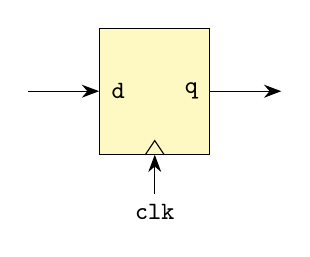
\begin{tikzpicture}[x=1cm,y=1cm]
  \node[reg,minimum width=14mm,minimum height=16mm] (ff) at (0,0) {};
  \node[font=\ttfamily\small,anchor=west] at ([xshift=1pt]ff.west) {d};
  \node[font=\ttfamily\small,anchor=east] at ([xshift=-1pt]ff.east) {q};
  \pic at ([xshift=0mm]ff.south) {clkmark};
  \draw[<-] (ff.west) -- ++(-0.9,0);
  \draw[->] (ff.east) -- ++(0.9,0);
  \draw[<-] (ff.south) -- ++(0,-0.5) node[below,font=\ttfamily\small] {clk};
\end{tikzpicture}
\hspace{8mm}
\begin{tikztimingtable}[timing/slope=0.1,timing/coldist=4pt,xscale=1.5,yscale=1.25,semithick]
  \code{clk} & 8{.5L .5H} \\
  \code{d}   & .2L 1.5H .5L .3H 1.2L 2H 2.3L \\
  \code{q}   & .5L 1H 2L 2H 2.5L \\
\extracode
  \begin{pgfonlayer}{background}
    \vertlines[cgray!50,dashed]{0.5,1.5,...,7.5}
  \end{pgfonlayer}
\end{tikztimingtable}
\caption{플립플롭. 왼쪽은 기호, 오른쪽은 동작이다. \code{q}는 상승 에지(점선)에서의 \code{d}를 받아 다음
에지까지 유지한다.}
\label{fig:g-dff}
\end{figure}

\section{레지스터 사이의 한 클럭}

\Relay 릴레이 계수기(\ref{sec:relay-counter}절)가 같은 문제를 이미 풀었다. 1을 더할 때 뒤집힐 비트를 정하는
올림 사슬은 비트 자신을 보고 있다. 비트가 뒤집히는 동안 사슬이 흔들리면 결과가 릴레이들의 빠르기 경쟁에
달린다. 계수기 보드는 비트마다 릴레이 둘과 두 상의 클럭으로 이를 막았다(그림~\ref{fig:r-counter}).
\code{NCK} 동안 마스터가 슬레이브의 반대값, 곧 ``뒤집으면 될 값''을 미리 만들어 두고, 슬레이브는 자기 유지로
현재 값을 붙든다. \code{CK} 동안 사슬이 닿은 비트의 슬레이브가 마스터의 값을 받는데, 사슬은 그동안 움직이지
않는 마스터의 접점으로만 이루어져 있다. \code{CK}와 \code{NCK}는 릴레이 하나의 한 극에서 나오므로 결코 동시에
켜지지 않는다(\ref{sec:relay-bbm}절). 그래서 계수기의 값은 \code{CK} 펄스에서만 움직인다.

FPGA의 플립플롭은 흔히 이 짝을 한 부품 안에 넣은 꼴로 만든다. 입력을 받아 두는 쪽과 내보내는 쪽이 클럭의
두 상에서 번갈아 열리고, 바깥에서 보면 값이 상승 에지 한 순간에 넘어간다. 릴레이식에서 보드 위에 직접 짜던
마스터--슬레이브를 FPGA의 설계자는 짤 필요가 없다. 플립플롭을 쓰면 이미 들어 있다.

이렇게 보면 동기식 회로의 모든 부분은 그림~\ref{fig:g-rcr}의 꼴로 볼 수 있다. 레지스터에서 나온 값이 조합
논리를 지나 다음 레지스터(같은 레지스터일 수도 있다)의 입력에 도착한다.

\begin{figure}[ht]
\centering
\begin{tikzpicture}[x=1cm,y=1cm]
  \node[reg,minimum height=14mm] (r1) at (0,0) {레지\\스터};
  \node[cloud,minimum width=44mm,minimum height=14mm] (c) at (4.2,0) {조합 논리\\{\footnotesize 지연 $t_{\mathrm{logic}}$}};
  \node[reg,minimum height=14mm] (r2) at (8.4,0) {레지\\스터};
  \draw[->] (r1) -- (c); \draw[->] (c) -- (r2);
  \draw[<-] (r1.south) -- ++(0,-0.6) coordinate (k1);
  \draw[<-] (r2.south) -- ++(0,-0.6) coordinate (k2);
  \draw (k1) -- (k2) node[midway,below,font=\ttfamily\small] {clk};
  \pic at (r1.south) {clkmark}; \pic at (r2.south) {clkmark};
  \draw[<->,cred] (0.6,1.15) -- node[above,note,text=cred] {이 구간의 지연이 클럭 주기보다 짧아야 한다} (7.8,1.15);
\end{tikzpicture}
\caption{동기식 회로의 기본 단위. 에지에서 출발한 값이 다음 에지 전에 도착해야 한다.}
\label{fig:g-rcr}
\end{figure}

\Why 이 꼴에서 동기식 설계의 유일한 시간 규칙이 나온다. \emph{한 에지에서 레지스터를 떠난 값은 조합
논리를 지나 다음 에지 전에 다음 레지스터에 도착해 있어야 한다.} 늦으면 다음 레지스터가 덜 계산된 값을
받아 적는다. 따라서 가장 느린 조합 논리 경로의 지연이 클럭 주기의 하한을, 곧 회로가 동작할 수 있는
최고 클럭 주파수를 정한다. 이 규칙만 지키면 조합 논리 안에서 값이 어떻게 출렁이든 상관이 없다.

릴레이식에서 같은 물음은 표~\ref{tab:t-rules}의 아홉 규칙 L1--L9가 되었다. 신호마다 릴레이 시간의 최악값을
더해 ``적어도 이만큼 기다려라''를 하나하나 따로 정해야 했다. 모두 하한이어서 기계가 느려지면 늘
안전했다(\ref{sec:t-bounds}절). 동기식 규칙도 같은 성질의 하한이다. 클럭을 늦추면 언제나 더 잘 지켜진다.
이 프로젝트의 FPGA 엔진도 처음 목표한 100~MHz에서 이 규칙을 지키지 못해 클럭을 50~MHz로
낮췄다(\ref{sec:timing}절). 다른 점은 규칙의 개수다. 동기식에서는 경로마다 같은 꼴의 규칙 하나이고, 설계
도구가 모든 경로의 지연을 계산해 확인해 준다. 설계자가 신경 쓸 시간의 단위가 ``나노초''에서 ``클럭 몇
번''으로 바뀌는 것이 동기식 설계의 이점이다.

\paragraph{클럭은 어디서 오는가.} 릴레이식은 박자를 만드는 데 보드 한 장을 썼다. 순서기의 555가 6.3~ms마다
4017을 한 칸 밀고, 열 칸이 한 위치라 한 위치가 63~ms다(\ref{sec:t-sequencer}절). 박자만은 릴레이가 아니라 전자
부품으로 만들었는데, 릴레이로 만든 지연은 최소를 보증할 수 없기 때문이다. 그리고 순서기는 그 박자 하나에서
\code{STROBE}, \code{JUDGE}, \code{CLEAR}, \code{CK}처럼 시각이 다른 신호 여럿을 따로 만들어 낸다. FPGA에서는
보드의 100~MHz 발진기에서 MMCM이라는 클럭 회로가 50~MHz를 만들고, 그 클럭 선 하나가 엔진의 모든 플립플롭에
들어간다. 한 주기는 20~ns다. 시각이 다른 신호를 클럭 선으로 따로 만들지 않는다. 클럭은 하나이고, ``이번
클럭에 무엇을 하는가''는 상태 기계가 정한다(\ref{sec:fsm}절).

\General 가장 단순한 예는 카운터다(그림~\ref{fig:g-counter}). 레지스터의 출력에 1을 더하는 조합 논리를
달고, 그 결과를 다시 레지스터의 입력에 넣는다. 에지마다 값이 1씩 커진다.

\begin{lstlisting}[language=SV,numbers=none]
logic [3:0] count;
always_ff @(posedge clk)
  if (reset) count <= 4'd0;
  else       count <= count + 4'd1;
\end{lstlisting}

\begin{figure}[ht]
\centering
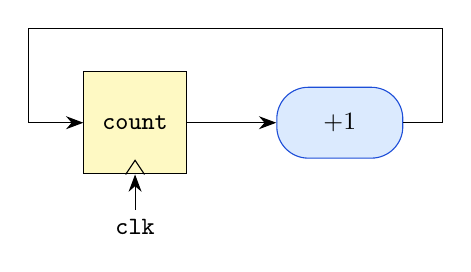
\begin{tikzpicture}[x=1cm,y=1cm]
  \node[reg,minimum height=13mm,minimum width=13mm] (r) at (0,0) {\code{count}};
  \node[cloud,minimum width=16mm] (a) at (2.6,0) {$+1$};
  \draw[->] (r) -- (a);
  \draw[->] (a.east) -- ++(0.5,0) |- (1.3,1.2) -| ([xshift=-7mm]r.west) -- (r.west);
  \pic at (r.south) {clkmark};
  \draw[<-] (r.south) -- ++(0,-0.45) node[below,font=\ttfamily\small] {clk};
\end{tikzpicture}
\hspace{6mm}
\begin{tikztimingtable}[timing/slope=0.1,timing/coldist=4pt,xscale=1.9,yscale=1.25,semithick]
  \code{clk}       & 5{.5L .5H} \\
  \code{count}     & .5D{0} 1D{1} 1D{2} 1D{3} 1D{4} .5D{5} \\
  \code{count+1}   & .5D{1} 1D{2} 1D{3} 1D{4} 1D{5} .5D{6} \\
\extracode
  \begin{pgfonlayer}{background}
    \vertlines[cgray!50,dashed]{0.5,1.5,...,4.5}
  \end{pgfonlayer}
\end{tikztimingtable}
\caption{카운터. 조합 논리는 ``다음 값''을 늘 계산하고 있고, 레지스터는 에지마다 그것을 받아 ``현재 값''으로
삼는다.}
\label{fig:g-counter}
\end{figure}

카운터에서 익혀 둘 것은 이름 두 개다. 레지스터에 담긴 \emph{현재 값}과, 조합 논리가 계산해 둔 \emph{다음
값}. 동기식 회로를 읽는 것은 결국 ``다음 값이 현재 값에서 어떻게 계산되는가''를 읽는 일이다. 릴레이 계수기도
같은 꼴이다. 슬레이브가 현재 값이고, 마스터의 거울과 올림 사슬이 다음 값을 만드는 부분이며, \code{CK} 펄스가
에지의 자리에 있다.

\Ours 봄베의 기준 RTL은 이 꼴 그대로다. \code{live\_q}가 676비트의 현재 상태를 담은 레지스터이고,
\code{live\_n}이 조합 논리(코드~\ref{lst:g-spread})가 계산한 다음 상태다. 이름 끝의 \code{\_q}와
\code{\_n}은 각각 레지스터의 출력과 다음 값(next)을 뜻하는 관례다. 카운터의 ``$+1$'' 자리에
``한 걸음 퍼뜨리기''가 들어갔을 뿐이다(그림~\ref{fig:g-liveloop}).

\begin{figure}[ht]
\centering
\begin{tikzpicture}[x=1cm,y=1cm]
  \node[reg,minimum height=16mm,minimum width=16mm] (r) at (0,0) {\code{live\_q}\\{\footnotesize 676비트}};
  \node[cloud,minimum width=44mm,minimum height=16mm] (f) at (4.6,0) {한 걸음 퍼뜨리기\\{\footnotesize 스크램블러 + 대각선 보드}};
  \draw[->] (r) -- (f);
  \draw[->] (f.east) -- ++(0.6,0) |- (2.3,1.5) node[pos=0.75,above,font=\footnotesize] {\code{live\_n}} -| ([xshift=-8mm]r.west) -- (r.west);
  \pic at (r.south) {clkmark};
  \draw[<-] (r.south) -- ++(0,-0.45) node[below,font=\ttfamily\small] {clk};
\end{tikzpicture}
\caption{\code{bombe\_core}의 뼈대. 그림~\ref{fig:g-counter}의 카운터와 같은 꼴이다.}
\label{fig:g-liveloop}
\end{figure}

릴레이식과 기어식에는 \code{live\_q}에 해당하는 기억이 없다. 676가닥은 전선 그 자체이고, 전압을 걸면 이어진
선이 저절로, 사실상 즉시 같은 전압이 된다(\ref{sec:f-current}절). 기억은 테스트 케이블의 26선에 달린 감지
릴레이뿐이다. 그 퍼짐을 FPGA의 게이트로 그대로 옮기면 출력이 자기 입력으로 돌아오는 고리가 되는데, 그런 고리는
한번 1이 되면 꺼지지 않고 설계 도구가 지연을 계산할 수도 없다. 그래서 676가닥 전부에 플립플롭을 하나씩 두어
고리를 끊고, 클럭마다 한 걸음씩 퍼뜨린다(\ref{sec:f-rounds}절). 전류가 공짜로 하던 일에 676비트의 기억과
걸음 수만큼의 클럭을 치르는 셈이다(\ref{sec:f-cost}절). 이 설계 결정은 \ref{ch:rtl-core}장에서 자세히 다룬다.

\section{\texorpdfstring{\code{<=}와 \code{=}}{<=와 =}: 동시에 갱신한다는 것}

\Relay 릴레이식의 계수기들은 한 위치에 한 번, 같은 \code{CK} 펄스 안에서 함께 움직인다(\ref{sec:relay-counter}절의
``계수 규칙의 배치''). 자리들 사이에 순서가 없다. 예를 들어 $a_3$는 ``$l \ne 25$''일 때만 오르는데,
이 조건은 $l$ 자리의 마스터 접점이 만든다. $l$ 자신도 같은 펄스에서 바뀌지만, 마스터는 \code{CK} 동안 움직이지
않으므로 $a_3$가 보는 것은 언제나 펄스 직전의 $l$이다. 같은 규칙을 차례로 실행되는 Rust로 적은
코드~\ref{lst:r-counters}는 다르다. \code{l\_wraps}와 \code{m\_wraps}를 맨 앞에서 옛 값으로 계산해 두고 나서야
값들을 바꾼다. 프로그램은 옛 값을 따로 적어 두어야 하고, 릴레이 계수기는 마스터가 옛 값을 붙들고 있으므로 그럴
필요가 없다.

SystemVerilog에는 대입 기호가 둘 있다. 레지스터를 기술하는 \code{always\_ff} 안에서는 \code{<=}(논블로킹
대입)를, 조합 논리를 기술하는 \code{always\_comb} 안에서는 \code{=}(블로킹 대입)를 쓴다.

\Why 클럭 에지에서 모든 레지스터는 \emph{동시에} 값을 바꾼다. 그러므로 어떤 레지스터의 새 값을 계산할 때
쓰이는 다른 레지스터의 값은 모두 \emph{에지 직전의} 값이어야 한다. \code{<=}는 바로 그 뜻이다. ``오른쪽을
지금의 값으로 계산해 두었다가, 에지에서 한꺼번에 왼쪽에 넣는다.'' 릴레이 계수기의 마스터가 하던 일을 문법
하나로 적은 것이다. 반면 \code{=}는 조합 논리를 적을 때 ``이 전선은 이 식의 결과다''를 차례로 이어 적기 위한
것이다(코드~\ref{lst:g-scr}의 \code{x}처럼).

\General 두 레지스터의 값을 맞바꾸는 회로를 보자.

\begin{lstlisting}[language=SV,numbers=none]
always_ff @(posedge clk) begin
  a <= b;
  b <= a;
end
\end{lstlisting}

프로그램이라면 첫 줄에서 \code{a}가 덮어써지므로 임시 변수가 필요하다. 회로에서는 필요 없다. 두 줄 모두
에지 직전의 값을 읽고, 에지에서 동시에 쓴다. 그림으로는 두 레지스터의 출력이 서로의 입력에 이어져 있을
뿐이다(그림~\ref{fig:g-swap}).

\begin{figure}[ht]
\centering
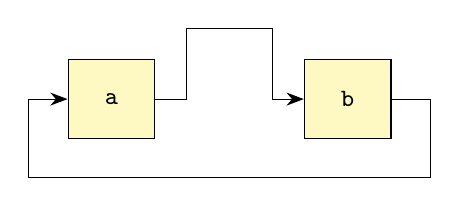
\begin{tikzpicture}[x=1cm,y=1cm]
  \node[reg,minimum width=11mm] (a) at (0,0) {\code{a}};
  \node[reg,minimum width=11mm] (b) at (3,0) {\code{b}};
  \draw[->] (a.east) -- ++(0.4,0) |- (1.5,0.9) -| ([xshift=-4mm]b.west) -- (b.west);
  \draw[->] (b.east) -- ++(0.5,0) |- (1.5,-1.0) -| ([xshift=-5mm]a.west) -- (a.west);
\end{tikzpicture}
\hspace{10mm}
\begin{tikztimingtable}[timing/slope=0.1,timing/coldist=4pt,xscale=1.8,yscale=1.25,semithick]
  \code{clk} & 5{.5L .5H} \\
  \code{a}  & .5D{3} 1D{8} 1D{3} 1D{8} 1D{3} .5D{8} \\
  \code{b}   & .5D{8} 1D{3} 1D{8} 1D{3} 1D{8} .5D{3} \\
\extracode
  \begin{pgfonlayer}{background}
    \vertlines[cgray!50,dashed]{0.5,1.5,...,4.5}
  \end{pgfonlayer}
\end{tikztimingtable}
\caption{맞바꾸기. 두 레지스터가 같은 에지에서 서로의 옛 값을 받는다.}
\label{fig:g-swap}
\end{figure}

\Ours \code{bombe\_core}에서 상태를 갱신하는 부분은 다음과 같다. 세 줄의 \code{<=}는 차례로 일어나는
일이 아니라 같은 에지에서 한꺼번에 일어나는 일이다. \code{iterations + 16'd1}에 쓰인 \code{iterations}도,
조건식의 \code{live\_q}도 모두 에지 직전의 값이다. 릴레이 계수기의 자리들이 한 \code{CK} 펄스에서 함께 오르는
것과 같다.

\begin{lstlisting}[language=SV,numbers=none]
SPREAD: begin
  live_q     <= live_n;
  iterations <= iterations + 16'd1;
  if (live_n == live_q || (early_exit && test_n == FULL)) begin
    state <= IDLE;
    done  <= 1'b1;
  end
end
\end{lstlisting}

\section{``차례로''는 상태 기계로 만든다}\label{sec:fsm}

\Relay 테스트 레지스터는 한 위치마다 \code{STROBE}, \code{JUDGE}, \code{CLEAR}를 이 차례로 받아야
한다(\ref{sec:t-register}절). 붙잡고, 판정하고, 지우는 표본 유지의 순서다. 이 차례를 만드는 장치가 기계마다
있다.
\begin{itemize}
\item \textbf{릴레이식의 순서기}(\ref{sec:t-sequencer}절). 4017의 출력 Q0--Q9 가운데 늘 하나만 켜져 있고,
555의 틱마다 다음 칸으로 넘어간다. ``지금 몇 번째 단계인가''를 이 칩이 기억한다. 단계마다 무엇을 내보낼지는
Q 몇 개를 다이오드 OR로 묶은 창이 정한다. \code{STROBE}는 Q0--Q1, \code{JUDGE}는 Q3--Q4, \code{CLEAR}는
Q6--Q8이고, Q9에서 링이 주차한다(그림~\ref{fig:t-ring}). 4017은 전자 칩이지만, 그 위에 얹힌 조건은 릴레이가
붙든다. \code{CK} 결정 릴레이는 Q6에서 \code{RUN}을 보고 붙어 Q6--Q8 동안 스스로를 붙들고, 한 걸음 버튼의
\code{KSA}와 \code{KSC}는 ``한 바퀴만 돈다''를 기억한다.
\item \textbf{기어식의 슬롯 원판}(\ref{sec:t-gear}절). 상태를 기억하는 부품이 따로 없다. 주기 축이 돈 각도가
곧 ``지금 몇 번째 단계인가''이고, 세 트랙의 슬롯이 단계마다의 출력이다(그림~\ref{fig:t-slots}). 각도로 만든
상태 기계인 셈이다. 그래도 각도만으로는 알 수 없는 사실, 곧 ``이번 주기에 \code{STROBE}를 냈는가''는 따로
기억해야 해서 제어 보드는 \code{CYC}와 \code{SEEN} 두 비트를 둔다. 실제 회로에서 이 둘은 D 플립플롭
두 개다(\ref{sec:gk-gates}절).
\end{itemize}

\Why 회로는 모든 것이 동시에 동작하므로, ``먼저 이것을 하고 그다음에 저것을 한다''는 순서는 저절로
생기지 않는다. 순서가 필요하면 ``지금 몇 번째 단계인가''를 기억하는 레지스터를 두고, 단계에 따라 다른
동작을 하게 한다. 이것이 \term{상태 기계}{finite state machine, FSM}다. 4017의 켜진 출력 하나가 바로 그
기억이었다. 프로그램에서는 처리 장치가 ``지금 몇 번째 줄인가''를 대신 기억해 주지만, 회로에서는 설계자가 그
기억을 직접 만든다.

\General 버튼을 누르면 LED를 정해진 시간 동안 켜 두는 회로를 생각하자. 상태는 둘이다. 기다리는
\code{IDLE}과 켜 두는 \code{ON}. \code{IDLE}에서 버튼이 눌리면 타이머를 0으로 하고 \code{ON}으로 간다.
\code{ON}에서는 클럭마다 타이머를 올리다가 정해진 값이 되면 \code{IDLE}로 돌아간다
(그림~\ref{fig:g-fsm} 왼쪽). 상태를 담는 방법은 여럿이다. 4017처럼 상태마다 선을 하나씩 두고 하나만 켜는
방법도 있고, 상태에 번호를 매겨 이진수로 담는 방법도 있다. 어느 쪽이든 상태를 담는 것은 레지스터이고, 다음
상태를 정하는 것은 조합 논리다.

\Ours \code{bombe\_core}의 상태 기계도 상태가 둘이고 구조가 같다(그림~\ref{fig:g-fsm} 오른쪽).
\code{IDLE}에서 시작 신호가 오면 상태를 초기화하고 \code{SPREAD}로 간다. \code{SPREAD}에서는 클럭마다 한
걸음씩 퍼뜨리다가 더 변하지 않으면 완료를 알리고 \code{IDLE}로 돌아간다. 타이머 대신 ``변화가 없는가''가
끝내는 조건일 뿐이다.

릴레이식의 순서와 나란히 놓으면 차이가 보인다. \code{IDLE}에서 \code{start}를 본 에지 하나에서 세 가지가 함께
일어난다(\ref{ch:rtl-core}장). 스크램블러들이 내놓은 치환표를 레지스터에 붙잡고, 676비트를 모두 0으로 지우고,
전압을 거는 선 하나만 1로 한다. 릴레이식에서는 지우기(\code{CLEAR})와 전압 걸기(\code{STROBE})가 서로 다른
박자였다. 감지 릴레이가 다 놓일 만큼 \code{CLEAR}를 길게 끌어야 했고, 유지 버스가 다시 살아난 뒤에야 다음
\code{STROBE}를 걸 수 있었다(표~\ref{tab:t-rules}의 L5, L6). 플립플롭은 모두 같은 에지에서 바뀌므로 그런
기다림이 없다. 판정도 따로 박자를 받지 않는다. 끝난 뒤의
\code{test\_q}가 다 찼는가를 보는 조합 논리 한 줄이다. 또 하나, 릴레이식의 한 위치는 링이 한 바퀴 도는
63~ms로 늘 같지만, \code{SPREAD}는 고정점에 닿을 때까지 머물므로 위치마다 걸음 수가
다르다(\ref{sec:f-rounds}절).

\begin{figure}[ht]
\centering
\begin{tikzpicture}[x=1cm,y=1cm,
   st/.style={draw,circle,minimum size=14mm,fill=cgreenbg,draw=cgreen,font=\small\ttfamily},
   sb/.style={draw,circle,minimum size=14mm,fill=cbluebg,draw=cblue,font=\small\ttfamily}]
  \node[font=\small\bfseries] at (1.8,2.4) {일반적인 예: LED 타이머};
  \node[st] (i) at (0,0) {IDLE};
  \node[st] (o) at (3.6,0) {ON};
  \draw[->] (i) to[bend left=25] node[above,note] {버튼 눌림\\타이머 $\leftarrow 0$} (o);
  \draw[->] (o) to[bend left=25] node[below,note] {타이머 = 끝값} (i);
  \draw[->] (o) to[out=30,in=-30,looseness=5] node[right,note] {타이머 $+1$} (o);
  \begin{scope}[xshift=8.6cm]
  \node[font=\small\bfseries] at (1.8,2.4) {\code{bombe\_core}};
  \node[sb] (i2) at (0,0) {IDLE};
  \node[sb] (s2) at (3.6,0) {SPREAD};
  \draw[->] (i2) to[bend left=25] node[above,note] {\code{start}\\상태 초기화} (s2);
  \draw[->] (s2) to[bend left=25] node[below,note] {변화 없음: \code{done}} (i2);
  \draw[->] (s2) to[out=30,in=-30,looseness=5] node[right,note] {한 걸음} (s2);
  \end{scope}
\end{tikzpicture}
\caption{상태 기계 두 개. 상태를 기억하는 것도 레지스터이고, 화살표는 ``다음 상태''를 정하는 조합 논리다.}
\label{fig:g-fsm}
\end{figure}

\section{정리}

\begin{itemize}
\item 회로는 조합 논리(계산)와 레지스터(기억)로 이루어진다. 릴레이식의 접점 나무와 자기 유지 릴레이가 각각
그 짝이다.
\item 레지스터는 클럭 에지에서만 값을 바꾸고, 모든 레지스터가 동시에 바꾼다. 릴레이 계수기가
마스터--슬레이브와 \code{CK}/\code{NCK}로 만들던 성질이 플립플롭 하나에 들어 있다.
\item 설계자가 적는 것은 ``현재 값에서 다음 값이 어떻게 나오는가''다.
\item 레지스터 사이의 조합 논리는 한 클럭 주기 안에 끝나야 한다. 이 제약이 최고 속도를 정한다. 릴레이식의
L1--L9처럼 하한이어서, 클럭을 늦추면 언제나 더 잘 지켜진다.
\item 순서가 필요하면 상태 기계를 만든다. 릴레이식은 링 계수기로, 기어식은 원판의 각도로, FPGA는 상태
레지스터로 ``지금 몇 번째 단계인가''를 기억한다.
\end{itemize}

표~\ref{tab:g-sync-map}은 이 장의 대응을 한데 모은 것이다.

\begin{table}[ht]
\centering
\caption{릴레이식과 FPGA에서 계산, 기억, 시간을 맡는 것.}
\label{tab:g-sync-map}
\small
\begin{tabular}{>{\raggedright\arraybackslash}p{24mm}>{\raggedright\arraybackslash}p{58mm}>{\raggedright\arraybackslash}p{50mm}}
\toprule
& 릴레이식 & FPGA \\
\midrule
기억 없는 계산 & 접점 나무, 이진 시프터 & 조합 논리 \\
1비트 기억 & 자기 유지 릴레이(감지 릴레이, 계수기의 슬레이브) & 플립플롭 \\
값이 넘어가는 순간 & \code{CK} 펄스(마스터--슬레이브, \code{CK}/\code{NCK}) & 클럭의 상승 에지 \\
시간 기준 & 순서기의 555와 4017, 한 틱 6.3~ms & 클럭 선 하나, 50~MHz \\
시간 규칙 & L1--L9, 신호마다 따로 정한 하한 & 경로마다 ``지연 $<$ 클럭 주기'' \\
순서 & 링 계수기 Q0--Q9와 상태 릴레이 & 상태 레지스터와 상태 기계 \\
\bottomrule
\end{tabular}
\end{table}

\chapter{자원: 회로는 공간을 차지한다}\label{ch:resources}

릴레이식 봄베에서 회로의 크기는 눈에 보인다. 6유닛에 릴레이가 3,455개 들고(테스트 레지스터 제외), 시프터 보드
한 장은 릴레이 130개를 싣느라 $250 \times 228$~mm가 되었으며, 기계의 폭은 1.88~m다. 켜져 있는 코일은 내내
전력을 열로 바꾸고(\ref{sec:el-power}절), 6유닛의 코일이 평균 0.21--0.31~kW를 쓴다. 회로를 하나 더하면 릴레이를 사서 기판에 꽂아야 하고,
기판과 전원과 팬이 함께 커진다. FPGA에서도 회로는 공간을 차지한다. 다만 그 공간은 칩 안에 미리 깔려 있는
부품의 수이고, 눈에 보이지 않는다.

회로의 비용은 둘이다. 부품이 차지하는 \emph{자원}과 신호가 지나는 데 걸리는 \emph{시간}. 이 장은 자원을 본다.
릴레이식에서 무엇이 릴레이를 많이 먹었는지를 먼저 떠올리고, FPGA 안에 어떤 부품이 있으며 코드가 그 부품을
얼마나 쓰는지 가늠하는 법으로 넘어간다. 이 감각이 없으면 \ref{ch:lesson}장의 사고가 난다.

\section{FPGA 안에 있는 것}

\Relay 릴레이식 봄베는 모든 보드를 극이 둘인 전환 접점 릴레이(DPDT) 한 종류로 짓는다(\ref{sec:relay-one}절).
논리는 접점의 직렬과 병렬로 만들고(\ref{sec:relay-logic}절), 1비트 기억은 자기 유지로 만든다(\ref{sec:relay-latch}절).
그래서 크기를 재는 단위가 릴레이의 개수다. 계수기 한 자리(5비트)가 릴레이 11개, 위치 표시 한 자리가 13개, 시프터
보드 한 장이 130개다(\ref{ch:relay-machine}장). 부품은 설계가 요구하는 만큼 사서 꽂는다. 그 대신 그것을 담을
그릇이 있다. 기계의 프레임에는 유닛 자리가 12개 있고, 먼저 만드는 6유닛은 그 절반을 채운다.

\Why FPGA는 만들어진 뒤에 회로를 바꿀 수 있는 칩이다. 게이트를 그때그때 새로 만들 수는 없으므로,
FPGA는 ``어떤 논리 함수로든 설정할 수 있는 작은 부품''을 수만 개에서 수십만 개 깔아 두고 그 사이를
설정 가능한 배선으로 잇는다. 그 작은 부품이 \term{LUT}{look-up table, 조회표}다. 릴레이식이 한 종류의 릴레이로
모든 것을 지은 것처럼, FPGA는 몇 종류 안 되는 범용 부품으로 모든 것을 짓는다. 다른 점은 부품의 수다. 칩마다
정해져 있고, 설계가 그 안에 들어가거나 들어가지 않거나 둘 중 하나다.

LUT는 이름 그대로 표다. 입력이 6개인 LUT(LUT6)는 $2^6 = 64$칸짜리 1비트 메모리이고, 입력 6비트를 주소로
삼아 그 칸의 값을 내놓는다. 64칸에 무엇을 적어 두느냐에 따라 입력 6개의 \emph{어떤} 논리 함수든 된다
(그림~\ref{fig:g-lut}). 합성 도구가 하는 일은 설계자가 적은 논리를 6입력 이하의 조각으로 쪼개 LUT에
하나씩 담는 것이다.

셈법이 릴레이와 다르다. 접점 회로에서는 식이 복잡할수록 접점이 늘었다. AND 하나에 직렬 접점 하나, OR 하나에
병렬 갈래 하나다. LUT에서는 식의 모양이 값을 정하지 않는다. 64칸 표에는 무엇이든 적을 수 있기 때문이다.

\begin{figure}[ht]
\centering
\begin{tikzpicture}[x=1cm,y=1cm]
  % 진리표
  \node[font=\small\bfseries] at (1.5,3.45) {LUT에 적힌 표 (일부)};
  \matrix[matrix of nodes,nodes={font=\ttfamily\footnotesize,minimum width=5mm,minimum height=4.2mm,inner sep=0pt},
          column sep=0pt,row sep=0pt] (m) at (1.5,0.9) {
     a & b & c & |[text=cgray]|\dots & {} & y \\
     0 & 0 & 0 & {} & {} & 0 \\
     0 & 0 & 1 & {} & {} & 1 \\
     0 & 1 & 0 & {} & {} & 0 \\
     0 & 1 & 1 & {} & {} & 1 \\
     1 & 0 & 0 & {} & {} & 0 \\
     1 & 0 & 1 & {} & {} & 1 \\
     1 & 1 & 0 & {} & {} & 1 \\
     1 & 1 & 1 & {} & {} & 1 \\
  };
  \draw (m-1-1.south west) -- (m-1-6.south east);
  \draw (m-1-5.north east) -- (m-9-5.south east);
  \node[note] at (1.5,-1.85) {\code{y = (a \& b) | c}};
  % LUT 기호
  \begin{scope}[xshift=6.6cm]
  \node[font=\small\bfseries] at (1.6,2.9) {LUT6 하나};
  \node[draw,fill=cbluebg,draw=cblue,minimum width=22mm,minimum height=30mm,align=center] (lut) at (1.6,0.8) {64칸\\메모리};
  \foreach \i/\l in {0/a,1/b,2/c,3/{},4/{},5/{}} {
    \draw[<-] ([yshift=11mm-\i*4.4mm]lut.west) -- ++(-0.8,0) node[left,font=\ttfamily\footnotesize] {\l};
  }
  \draw[->] (lut.east) -- ++(0.8,0) node[right,font=\ttfamily\footnotesize] {y};
  \node[note] at (1.6,-1.4) {입력 6비트가 주소, 출력은 그 칸의 값};
  \end{scope}
  % FF
  \begin{scope}[xshift=11.6cm]
  \node[font=\small\bfseries] at (1.2,2.9) {짝을 이루는 플립플롭};
  \node[reg,minimum width=12mm,minimum height=14mm] (ff) at (1.2,0.8) {FF};
  \pic at (ff.south) {clkmark};
  \draw[<-] (ff.west) -- ++(-0.6,0);
  \draw[->] (ff.east) -- ++(0.6,0);
  \node[note] at (1.2,-1.4) {1비트 기억};
  \end{scope}
\end{tikzpicture}
\caption{LUT는 작은 메모리로 만든 만능 게이트다. 그림~\ref{fig:g-assign}의 게이트 두 개는 LUT 하나에
들어간다(입력 세 개만 쓴다).}
\label{fig:g-lut}
\end{figure}

\General \code{y = (a \& b) | c}는 입력이 셋이므로 LUT 하나다. 접점으로 만들면 \code{a}와 \code{b}의 직렬에
\code{c}를 병렬로 단 접점 셋이지만, LUT에서는 게이트가 몇 개인지가 중요하지 않다.
중요한 것은 \emph{출력 하나가 입력 몇 개에 의존하는가}다. 입력이 여섯 이하이면 아무리 복잡한 식도
LUT 하나이고, 일곱 이상이면 LUT 여러 개를 엮어야 한다.

FPGA에는 LUT 말고도 몇 가지 부품이 있다(표~\ref{tab:g-res}).

\begin{table}[ht]
\centering
\caption{FPGA의 주요 자원. 수량은 이 프로젝트의 대상 칩 두 종의 대략적인 값이다.}
\label{tab:g-res}
\small
\begin{tabularx}{\linewidth}{l>{\raggedright\arraybackslash}X>{\raggedright\arraybackslash}p{27mm}>{\raggedright\arraybackslash}p{24mm}}
\toprule
자원 & 하는 일 & XC7A200T (Nexys Video) & XC7Z020 (PYNQ) \\
\midrule
LUT & 6입력 이하의 임의의 논리 함수. 조합 논리가 여기에 담긴다 & 약 13만 4천 & 약 5만 3천 \\
플립플롭(FF) & 1비트 기억. 레지스터가 여기에 담긴다 & LUT마다 딸려 있다 & \\
분산 RAM (LUT RAM) & LUT의 64칸 메모리를 그대로 작은 RAM으로 쓰는 것. 작고 빠른 표에 알맞다 & LUT의 일부를 전용 & \\
블록 RAM & 큰 메모리 전용 블록(수만 비트 단위). 읽는 데 한 클럭이 든다 & 365개 & 140개 \\
DSP 블록 & 곱셈기. 신호 처리에 쓰인다 & (이 프로젝트에서는 쓰지 않는다) & \\
\bottomrule
\end{tabularx}
\end{table}

\Ours 봄베의 회로에는 곱셈이 없고 큰 메모리도 필요 없다. 자원의 거의 전부가 LUT(전파 논리와 치환 계산)와
플립플롭(676비트 상태와 치환표)이다. 그래서 이 프로젝트에서 ``회로가 큰가''는 곧 ``LUT를 몇 개 쓰는가''다.

두 기계가 무엇을 세는지 나란히 놓으면 표~\ref{tab:g-res-count}와 같다. 릴레이 하나와 LUT 하나는 같은 크기의
부품이 아니므로 수를 직접 견줄 수는 없다. 볼 것은 \emph{어디에} 부품이 드는가다. 눈에 띄는 차이가 기억이다.
릴레이식은 676가닥의 상태를 기억하지 않는다. 전류가 한순간에 퍼지므로, 선의 상태 가운데 붙들어 두는 것은
결과를 읽는 테스트 레지스터의 26비트뿐이다(\ref{sec:t-register}절). FPGA는 한 걸음씩 퍼뜨리므로(\ref{sec:f-rounds}절) 676가닥 전부의 상태를
플립플롭에 담아 두어야 한다.

\begin{table}[ht]
\centering
\caption{두 기계의 크기를 재는 단위. 릴레이식은 6유닛의 값(보고서의 릴레이 수 표, 테스트 레지스터 제외), FPGA는
엔진 한 대를 합성한 단계의 값이다(\ref{ch:lesson}장).}
\label{tab:g-res-count}
\small
\begin{tabularx}{\linewidth}{l >{\raggedright\arraybackslash}X >{\raggedright\arraybackslash}X}
\toprule
& 릴레이식 & FPGA 엔진 \\
\midrule
부품 & 릴레이 3,455개. 그 가운데 시프터가 3,120개 & LUT 41,040개 \\
기억 & 자기 유지 릴레이. 선의 상태로 붙드는 것은 테스트 레지스터의 26비트 & 플립플롭 7,338개. 676가닥의 상태 전부를 포함 \\
표 & 배선 카드의 구리. 능동 부품이 없다 & LUT RAM 2,858개 \\
그릇 & 유닛 12자리의 프레임(폭 1.88~m) & 칩의 LUT 약 13만 4천 개 \\
따라오는 대가 & 코일의 전력과 열 (6유닛 평균 0.21--0.31~kW) & 칩이 찰수록 배선이 길어진다 (\ref{ch:pipeline}장) \\
\bottomrule
\end{tabularx}
\end{table}

\section{선택 회로는 비싸다}\label{sec:mux-cost}

회로에서 LUT를 가장 많이 잡아먹는 것은 덧셈도 비교도 아니고 \term{선택 회로}{multiplexer, mux}다.
여러 입력 가운데 하나를 골라 내보내는 회로다. 릴레이식에서도 사정이 같았다.

\Relay 릴레이식에서 ``여럿 가운데 하나를 고르는'' 회로는 두 번 나왔다. 하나는 위치 표시의 접점
나무다(\ref{sec:relay-tree}절). 5비트 값을 보고 램프 26개 가운데 하나에 전압을 보낸다. 전환 접점 하나가 길을
둘로 가르므로 26갈래에는 접점 25개가 든다. 고를 대상이 $n$개이면 접점이 $n-1$개, 대상의 수에 비례한다. 다른
하나는 이진 시프터다(\ref{sec:relay-shifter}절). 선마다 ``0--25칸 가운데 몇 칸 밀린 선으로 이을까''를 고르는 회로다.
위치마다 따로 배선하면 유닛 하나에 접점이 4,056개 들지만, 밀기를 1·2·4·8·16칸의 단으로 나누고 이웃한 밀기를
합쳐 1,040개(릴레이 520개)로 줄였다. 그렇게 줄이고도 6유닛의 릴레이 3,455개 가운데 3,120개가 시프터다.
릴레이식에서 가장 비싼 회로가 선택 회로였다.

\Why 선택 회로의 출력은 \emph{모든} 데이터 입력과 선택 신호에 의존한다. 넷 중 하나를 고르는 4:1 선택
회로는 데이터 4비트와 선택 2비트, 모두 여섯 입력이므로 LUT6 하나에 꼭 맞는다. 그보다 큰 선택 회로는
4:1을 층층이 쌓아야 한다. 16:1은 4:1 네 개로 16개를 4개로 줄이고 다시 4:1 하나로 고르므로 LUT 다섯 개다.
이런 식으로 $N$개 가운데 하나를 고르려면 LUT가 대략 $N/3$개 든다($N/4 + N/16 + \cdots$). 접점 나무와 같은
셈이다. 접점 나무의 갈림 하나는 2:1 선택이어서 $n-1$개가 들고, LUT 하나는 4:1 선택이어서 그 삼분의 일쯤 든다.
어느 쪽이든 고를 대상의 수에 비례한다. 그리고 이것은 \emph{출력 1비트당}의 값이다(그림~\ref{fig:g-muxtree}).
시프터의 한 단이 코일 신호 하나를 나눠 쓰면서도 26선마다 접점을 하나씩 따로 두는 것과 같다. 고르는 신호는
함께 쓰지만, 골라지는 데이터는 비트마다 제 길이 있어야 한다.

\begin{figure}[ht]
\centering
\begin{tikzpicture}[x=1cm,y=1cm]
  \node[font=\small\bfseries] at (0.9,2.6) {4:1 = LUT 1개};
  \node[mux,minimum width=20mm] (m0) at (0.9,0.9) {4:1};
  \foreach \i in {0,1,2,3} { \draw[<-] ([yshift=7.5mm-\i*5mm]m0.west) -- ++(-0.6,0); }
  \draw[->] (m0.east) -- ++(0.5,0);
  \draw[<-] (m0.south) -- ++(0,-0.45) node[below,font=\footnotesize] {선택 2비트};
  \begin{scope}[xshift=5.2cm]
  \node[font=\small\bfseries] at (2.0,2.6) {16:1 = LUT 5개};
  \foreach \k/\yy in {0/2.0,1/1.0,2/0.0,3/-1.0} {
    \node[mux,minimum width=9mm,minimum height=5mm,font=\scriptsize] (a\k) at (0.8,\yy) {4:1};
    \foreach \i in {0,1,2,3} { \draw ([yshift=3mm-\i*2mm]a\k.west) -- ++(-0.35,0); }
  }
  \node[mux,minimum width=20mm] (b) at (3.4,0.5) {4:1};
  \foreach \k in {0,1,2,3} { \draw[->] (a\k.east) -- ++(0.5,0) |- ([yshift=7.5mm-\k*5mm]b.west); }
  \draw[->] (b.east) -- ++(0.5,0);
  \end{scope}
  \begin{scope}[xshift=11.3cm]
  \node[font=\small\bfseries] at (1.6,2.6) {크기의 어림 (출력 1비트당)};
  \node[font=\small,align=left,anchor=north west] at (-0.4,2.2) {
     \begin{tabular}{@{}rl@{}}
       4:1 & LUT 1개 \\
       16:1 & 5개 \\
       26:1 & 열 개 안팎 \\
       676:1 & 이백 개 이상 \\
     \end{tabular}};
  \end{scope}
\end{tikzpicture}
\caption{선택 회로의 크기. 고를 대상이 많아지면 그에 비례해 커진다. 접점 나무가 26글자에 접점 25개를 쓰는
것과 같은 셈법이다.}
\label{fig:g-muxtree}
\end{figure}

\paragraph{한 방향의 선택.} 다른 점이 하나 있다. 접점의 선택은 양방향이다. 시프터 보드 한 장이 가는 길의
밀기와 오는 길의 되돌림을 같은 릴레이의 두 극으로 함께 맡고, 같은 보드를 거꾸로 끼우면 반대로 민다
(\ref{sec:relay-shifter}절). FPGA의 선택 회로에는 방향이 있다(\ref{sec:hdl-direction}절). 입력 여럿 가운데 하나를
출력으로 내보낼 뿐, 출력 쪽에서 들어온 신호를 입력 쪽으로 돌려보내지 못한다. 거꾸로 지나는 길이 필요하면
선택 회로를 한 벌 더 둔다.

\General 선택 회로는 코드에서 눈에 잘 띄지 않는다. 다음 두 줄은 모두 선택 회로다. 특히 둘째 줄, 변수로
배열의 원소를 고르는 것은 프로그램에서는 가장 값싼 연산이지만 회로에서는 ``배열의 모든 원소를 선택 회로의
입력에 연결한다''는 뜻이다.

\begin{lstlisting}[language=SV,numbers=none]
assign y = sel ? a : b;      // 2:1 mux
assign z = table[index];     // (size of table):1 mux, for every bit of z
\end{lstlisting}

\Ours 봄베의 회로는 선택 회로투성이다. ``26글자 가운데 하나''를 고르는 일이 곳곳에 있기 때문이다.
로터를 통과하는 것은 배선표 26칸에서 한 칸을 고르는 일이고(5비트 폭의 26:1), 전파 논리에서 ``케이블 $a$의
$y$번 선''을 읽는 것도 선택이다. 코드~\ref{lst:g-spread}의 \code{live\_q[cable\_a + y]}가 그것인데,
여기서 고르는 대상은 26개가 아니라 676개다. 이 한 줄이 이 프로젝트의 가장 큰 사고의 원인이었다.
\ref{ch:lesson}장에서 다룬다.

릴레이식에는 이 선택이 없다. ``메뉴의 이 선은 케이블 $a$와 케이블 $b$를 잇는다''는 관람객이 메뉴 케이블을
잭에 꽂아 정한다(\ref{sec:bombe-one-page}절, \ref{sec:c-scrambler}절). 꽂힌 케이블은 구동 내내 그대로이므로 접점도 릴레이도 들지 않는다.
FPGA에는 꽂을 케이블이 없다. 메뉴를 설정값으로 받고, 그 설정값으로 케이블을 고르는 선택 회로가 생긴다.
사람이 손으로 하던 고르기가 회로가 되는 것이다. \ref{ch:lesson}장의 해결책은 이 고르기를 ``676개 가운데
하나''가 아니라 ``케이블 26개 가운데 하나, 그 안에서 선 26개 가운데 하나''로 나누는 것이다. 위치마다 따로 잇던
26가지를 1·2·4·8·16칸 다섯 단으로 나눈 시프터처럼, 큰 선택을 구조에 맞춰 작은 선택으로 나누면 싸진다.

\section{표는 메모리에 담는다}

\Relay 릴레이식에서 로터의 배선표는 배선 카드 $W$의 구리다(\ref{sec:relay-shifter}절,
\code{hardware/relay/wiring-cards}). 카드에는 커넥터와 장착 구멍 말고 부품이 없다. 로터 카드 한 장에 가는 길
26가닥과 오는 길 26가닥이 동선으로 그려져 있을 뿐이다. ``$i$번 핀으로 들어온 전류는 $W[i]$번 핀으로 나간다''가
그대로 표 조회다. 릴레이도 코일 전력도 들지 않고, 표를 바꾸려면 카드를 바꿔 꽂는다. 기어식에서는 같은 표가
드럼 기판의 안쪽 층에 있다(\ref{sec:gm-drum}절). 드럼으로 돌아오는 전류는 같은 배선을 거꾸로 지나므로
역방향 표 $W^{-1}$이 저절로 된다. 다만 두 기계 모두 \emph{계산해 둔} 표는 없다. 위치마다의 치환은 시프터의
접점이나 드럼의 회전이 그 자리에서 만들 뿐, 어디에도 적어 두지 않는다.

\Why 같은 계산을 되풀이하는 것보다 계산해 둔 결과를 표에서 읽는 편이 싸다. 프로그램에서도 쓰는 방법이지만
회로에서는 의미가 더 크다. 계산 회로는 쓰든 안 쓰든 자리를 차지하고 있는 반면, 메모리는 같은 양의 정보를
훨씬 좁은 자리에 담는다. FPGA에는 메모리가 두 종류 있다. LUT를 메모리로 쓰는 \term{분산 RAM}{distributed
RAM}은 작지만 주소를 주면 같은 클럭 안에 값이 나오고, \term{블록 RAM}{block RAM}은 크지만 읽는 데 한 클럭이
걸린다. FPGA의 표는 구리처럼 공짜가 아니다. 표 하나가 LUT나 플립플롭 몇 개를 차지한다. 그리고 거꾸로 흐르는
전류가 없으므로 역방향으로 읽을 표도 따로 담아야 한다.

\General 소리를 내는 회로가 사인파를 필요로 한다고 하자. 사인 함수를 계산하는 회로를 만드는 대신 한 주기의
값을 256칸짜리 표에 넣어 두고 차례로 읽어 낸다. 표는 블록 RAM 하나의 일부에 들어간다.

\Ours 로터의 배선표는 바뀌지 않는 상수 표다. 기준 RTL에서는 \code{wirings\_pkg}에 상수로 들어 있고
로터를 통과하는 함수가 그 표를 읽는다. FPGA 엔진은 구동을 시작할 때 고른 로터들의 정방향 표와 역방향 표,
반사판 표, 모두 아홉 장을 레지스터로 옮긴다. 한 클럭에 한 칸씩 234클럭이 든다(\ref{sec:e-loader}절).
릴레이식에서 배선 카드를 꽂는 일에 해당한다. 엔진은 한 걸음 더 나아가, 릴레이식이라면 위치마다 시프터가 새로
만들었을 스크램블러의 치환표를 미리 계산해 분산 RAM에 넣어 두고 읽어 쓴다. 다음 절의 주제다. 그 메모리는
메뉴의 선마다 하나씩 사본을 둔다(\ref{sec:e-ram}절). 릴레이식이 메뉴의 선마다 유닛을 하나씩 두는 것과 닮았다.

\section{자원과 시간을 맞바꾼다}\label{sec:tradeoff}

회로 설계에서 가장 자주 하는 결정은 ``부품을 더 쓰고 빨리 끝낼 것인가, 부품을 아끼고 오래 걸릴 것인가''다.
릴레이식에서는 거의 하지 않던 결정이다.

\Relay 릴레이식에는 이 거래의 여지가 거의 없다. 이어진 선을 전류로 찾으려면 메뉴의 연결이 \emph{모두 동시에}
있어야 한다(\ref{sec:f-current}절). 그래서 메뉴의 선마다 유닛이 하나씩 있어야 하고(\ref{sec:c-scrambler}절),
유닛 하나를 여러 선에 차례로 돌려 쓸 수 없다. 위치 하나의 시간도 릴레이의 개수가 아니라 릴레이가 넘어가고 붙는
시간이 정한다. 순서기의 한 주기, 63~ms다(\ref{sec:t-sequencer}절). 설계에서 저울질한 것은 릴레이 수와 시간이
아니라 릴레이 수와 다른 대가였다. 접점이 네 회로인 범용 릴레이를 쓰면 시프터의 릴레이가 절반(유닛당 260개)이
되지만, 코일 전력이 약 0.9~W여서 유닛 하나가 평균 100~W를 넘고 동작도 다섯 배 느리다(보고서의 릴레이 선정).
그래서 작은 릴레이를 많이 쓰는 쪽을 택했다. 뺄셈기 대신 차이를 직접 세는 계수기(\ref{sec:relay-counter}절)는
시간을 내주지 않고 구조만 바꿔 릴레이를 아낀 예다.

\Why 같은 계산을 하는 회로는 하나가 아니다. 계산에 필요한 연산을 전부 따로따로 부품으로 놓으면 한 클럭에
끝나지만 부품이 많이 든다. 부품 하나를 여러 클럭에 걸쳐 돌려 쓰면 부품은 적게 들지만 클럭이 여러 번
필요하다. 프로그램에서는 이 선택이 없다. 처리 장치가 하나이므로 언제나 뒤쪽이다.

FPGA에서 이 선택이 열리는 까닭은 \ref{sec:f-cost}절의 비교에 있다. 실물 기계의 위치 하나에는 연결을 한 번
바꾸고 전류를 한 번 거는 일밖에 없어서 쪼개어 나눠 쓸 시간이 없다. FPGA에서는 위치마다 클럭이 여러 번 들고,
클럭은 나노초 단위로 싸다. 그래서 회로 한 벌을 여러 클럭에 걸쳐 돌려 쓰고 부품을 아낄 수 있다.

\General 수 여덟 개의 합을 구한다고 하자(그림~\ref{fig:g-tradeoff}). 왼쪽은 덧셈기 일곱 개를 나무 모양으로
엮어 한 클럭에 답을 낸다. 오른쪽은 덧셈기 하나와 누산 레지스터 하나로 여덟 클럭에 걸쳐 하나씩 더한다.
신호 처리의 필터도 같다. 탭이 여덟 개인 필터는 곱셈기 여덟 개로 한 클럭에 계산할 수도 있고, 곱셈기 하나로
여덟 클럭에 걸쳐 계산할 수도 있다. 표본이 들어오는 속도가 느리면 뒤쪽으로 충분하다.

\begin{figure}[ht]
\centering
\begin{tikzpicture}[x=1cm,y=1cm,
   add/.style={draw,circle,fill=cbluebg,draw=cblue,minimum size=6mm,inner sep=0pt,font=\small}]
  \node[font=\small\bfseries] at (2.6,3.4) {병렬: 덧셈기 7개, 1클럭};
  \foreach \i in {0,...,7} { \node[font=\ttfamily\scriptsize] (x\i) at (\i*0.75,2.6) {x\i}; }
  \foreach \k/\a/\b in {0/0/1,1/2/3,2/4/5,3/6/7} {
    \node[add] (s\k) at (\k*1.5+0.375,1.7) {+};
    \draw[->] (x\a) -- (s\k); \draw[->] (x\b) -- (s\k);
  }
  \node[add] (t0) at (1.125,0.8) {+}; \node[add] (t1) at (4.125,0.8) {+};
  \draw[->] (s0) -- (t0); \draw[->] (s1) -- (t0); \draw[->] (s2) -- (t1); \draw[->] (s3) -- (t1);
  \node[add] (u) at (2.625,-0.1) {+};
  \draw[->] (t0) -- (u); \draw[->] (t1) -- (u);
  \draw[->] (u) -- ++(0,-0.6) node[below,font=\small] {합};
  \begin{scope}[xshift=9.0cm]
  \node[font=\small\bfseries] at (2.0,3.4) {직렬: 덧셈기 1개, 8클럭};
  \node[font=\ttfamily\small] (xin) at (-0.2,1.6) {x[i]};
  \node[add,minimum size=8mm] (p) at (1.3,1.6) {+};
  \node[reg,minimum width=14mm] (acc) at (3.3,1.6) {누산};
  \pic at (acc.south) {clkmark};
  \draw[->] (xin) -- (p); \draw[->] (p) -- (acc);
  \draw[->] (acc.east) -- ++(0.5,0) |- (2.3,0.5) -| (p.south);
  \draw[->] (acc.east) ++(0.5,0) -- ++(0.6,0) node[right,font=\small] {합};
  \node[note] at (2.0,-0.3) {클럭마다 수 하나를 더한다};
  \end{scope}
\end{tikzpicture}
\caption{같은 계산의 두 가지 구현.}
\label{fig:g-tradeoff}
\end{figure}

\Ours 봄베에서 이 선택은 스크램블러의 치환표를 언제, 어떻게 계산하는가에 나타난다.

실제 기계를 떠올려 보자. 봄베의 드럼 세 개 가운데 빠른 드럼은 계속 돌지만, 가운데 드럼은 빠른 드럼이 한 바퀴
돌 때 한 칸씩만, 느린 드럼은 그보다 더 드물게 움직인다. 26위치 동안 스크램블러의 ``안쪽''(가운데 로터, 왼쪽 로터, 반사판)은 그대로다.

\begin{itemize}
\item \textbf{기준 RTL}은 이 사실을 이용하지 않는다. 메뉴의 선마다 스크램블러 회로 전체(그림~\ref{fig:g-scr26})를
하나씩 두고 드럼 위치가 바뀔 때마다 26글자의 치환을 전부 다시 계산한다. 릴레이식과 같은 구조다. 릴레이식도
메뉴의 선마다 유닛을 하나씩 두고, 위치마다 시프터가 접점을 넘겨 치환을 새로 만든다. 릴레이식에서 그 값은
위치마다 접점이 넘어가는 시간이었고 그 시간은 어차피 63~ms 안에 들어 있었다. FPGA에서는 값이 공간으로 온다.
구조가 단순해서 맞는지 확인하기 쉽지만, 스크램블러 하나가 LUT 19,717개이므로 선이 16개인 메뉴에서는
스크램블러만으로 약 31만 5천 개다. 대상 칩(약 13만 4천 개)에 들어가지 않는다.
\item \textbf{FPGA 엔진}은 바뀌는 것만 다시 계산한다. 가운데 로터가 바뀔 때에만 안쪽 치환과 오른쪽 로터
26위치의 치환표를 여러 클럭에 걸쳐 계산해 분산 RAM에 넣어 두고, 위치마다 표에서 읽는다. 계산 회로는 한
벌만 있으면 되고 나머지는 메모리다.
\item \textbf{Rust 코어}도 같은 생각으로 짜여 있다. 가운데 로터가 바뀔 때만 표 26개를 다시 만든다
(\ref{ch:rust-bombe}장).
\end{itemize}

그림~\ref{fig:g-engine-idea}는 두 구조의 차이다. 엔진은 표를 만드는 데 클럭을 쓰지만 그것은 26위치에 한
번이다. 시간을 조금 내주고 LUT를 크게 돌려받았다. 엔진 전체는 LUT 41,040개에 들어간다. 엔진의 내부는
G부에서 다룬다.

\begin{figure}[ht]
\centering
\begin{tikzpicture}[x=1cm,y=1cm]
  \node[font=\small\bfseries] at (2.8,3.0) {기준 RTL: 위치마다 전부 다시 계산};
  \foreach \i/\yy in {0/2.1,1/1.3,2/0.5} {
    \node[blkb,minimum width=38mm,minimum height=6mm,font=\footnotesize] (s\i) at (2.2,\yy) {스크램블러 회로 (26글자분)};
    \draw[->] (s\i.east) -- ++(1.0,0);
  }
  \node at (2.2,-0.1) {$\vdots$};
  \node[note] at (2.2,-0.8) {메뉴의 선마다 한 벌 (최대 16벌)};
  \node[blkn,minimum width=10mm,minimum height=24mm] (sp) at (5.7,1.3) {전파};
  \begin{scope}[xshift=8.6cm]
  \node[font=\small\bfseries] at (3.1,3.0) {FPGA 엔진: 바뀔 때만 계산해 표에 저장};
  \node[blkb,minimum width=26mm,minimum height=10mm,font=\footnotesize] (calc) at (0.9,1.6) {치환 계산 회로\\(한 벌)};
  \node[reg,minimum width=22mm,minimum height=10mm,font=\footnotesize] (ram) at (3.9,1.6) {치환표\\(분산 RAM)};
  \node[blkn,minimum width=10mm,minimum height=24mm] (sp2) at (6.2,1.3) {전파};
  \draw[->] (calc) -- (ram); \draw[->] (ram) -- (sp2.west|-ram);
  \node[note] at (0.9,0.6) {가운데 로터가\\바뀔 때만 동작};
  \node[note] at (3.9,0.6) {위치마다 읽기};
  \end{scope}
\end{tikzpicture}
\caption{치환표를 얻는 두 가지 방법(개념도). 왼쪽은 릴레이식처럼 선마다 한 벌을 두고 위치마다 새로 만든다.}
\label{fig:g-engine-idea}
\end{figure}

같은 거래는 한 층 위에도 있다. 엔진 한 대는 로터 순서 하나를 맡으므로, 엔진을 두 대 두면 로터 순서 둘을
동시에 돈다. 배치와 배선을 마친 결과 한 대가 LUT 43,100개(32.2\%), 두 대가 83,257개(62.2\%)였고, 세 대이면 약
93\%가 되어 두 대로 정했다(\ref{sec:e-results}절). 릴레이식의 프레임에 유닛 자리가 12개뿐인 것처럼, 칩이라는
그릇의 크기가 나란히 둘 수 있는 수를 정한다.

\section{자원은 비싼 일에 든다}

두 기계에서 부품이 어디에 드는지 보면 \ref{sec:f-cost}절이 그대로 드러난다.

\begin{itemize}
\item \textbf{릴레이식}은 릴레이의 약 9할이 시프터, 곧 \emph{연결을 바꾸는} 회로다. 이어진 선을
찾는 데에는 릴레이가 하나도 들지 않는다. 메뉴 케이블과 대각선 보드는 구리이고, 릴레이가 드는 것은 찾은
결과를 읽고 판정하는 테스트 레지스터(감지 릴레이 26개와 판정·타이밍 릴레이 몇 개)뿐이다.
\item \textbf{FPGA 엔진}은 연결을 바꾸는 일을 표 읽기로 싸게 끝낸다. 크기를 좌우한 것은 \emph{이어진 선을
찾는} 전파 회로였다. 그 회로를 어떻게 적느냐에 따라 LUT가 약 40만 4천 개에서 41,040개로 달라졌다(\ref{ch:lesson}장).
\end{itemize}

물리가 공짜로 해 주던 일을 FPGA에서는 부품으로 짓는다. 그래서 FPGA 설계에서 자원을 아끼는 일은 대부분 그
일을 얼마나 싸게 짓는가의 문제다.

\section{정리}

\begin{itemize}
\item 릴레이식의 크기는 릴레이의 개수, 기판, 프레임, 코일의 열로 보인다. FPGA의 크기는 칩 안에 미리 깔린
부품을 몇 개 쓰는가다. 논리는 LUT에, 기억은 플립플롭에 담긴다. 회로의 크기는 주로 LUT의 수로 잰다.
\item LUT 하나는 입력 여섯 개까지의 함수다. 접점과 달리 식의 모양이 아니라 출력 하나가 의존하는 입력의 수가
크기를 정한다.
\item 변수로 무엇인가를 고르는 코드는 선택 회로이고, 고를 대상의 수에 비례해 커진다. 접점 나무가 $n$글자에
접점 $n-1$개를 쓰고 시프터가 릴레이식에서 가장 비쌌던 것과 같은 셈법이다. 큰 선택은 구조에 맞춰 작은 선택으로
나누면 싸진다.
\item 릴레이식의 표는 배선 카드와 드럼 기판의 구리여서 공짜이고 양방향이다. FPGA의 표는 메모리에 담기며,
되풀이되는 계산을 표로 만들어 두면 싸다.
\item 릴레이식은 연결이 모두 동시에 있어야 해서 자원과 시간을 맞바꿀 여지가 거의 없다. FPGA는 같은 계산을
부품을 많이 써서 빨리 할 수도, 적게 써서 천천히 할 수도 있다. 무엇이 자주 바뀌고 무엇이 드물게 바뀌는지를
보면 어디서 아낄지가 보인다.
\end{itemize}

\chapter{시간: 파이프라인과 타이밍 클로저}\label{ch:pipeline}

릴레이식 기계의 시간은 순서기가 정한다. 한 틱이 6.3~ms이고 열 틱이 한 위치다(\ref{sec:t-sequencer}절).
이 6.3~ms는 릴레이가 가장 느릴 때에도 \code{STROBE}, \code{JUDGE},
\code{CLEAR}의 규칙 L1--L9가 지켜지도록 계산해서 고른 값이다(\ref{ch:relay-timing}장). 물음은 하나다. 가장
느린 부품도 정해진 창 안에 일을 마치는가. 마치지 못하면 창을 넓히거나 회로를 바꾼다.

FPGA에도 같은 물음이 있다. \ref{ch:sync}장의 규칙을 다시 적으면, 레지스터 사이의 조합 논리는 한 클럭 주기
안에 끝나야 한다. 다른 점은 창이 밀리초가 아니라 나노초라는 것, 그리고 확인하는 것이 사람의 계산과
시뮬레이션이 아니라 설계 도구라는 것이다. 이 창을 가장 빠듯하게 쓰는 회로는 실물 기계에서 전류가 공짜로
하던 일, 곧 이어진 선을 찾는 회로다(\ref{sec:f-cost}절). 앞 장이 회로의 공간 비용을 다뤘다면 이 장은 시간
비용을 다룬다. 긴 일을 창에 맞게 나누는 방법(파이프라인), 회로가 칩 위에 놓이는 과정(합성, 배치, 배선),
규칙을 지켰는지 확인하는 과정(타이밍 클로저)의 차례로 본다.

\section{파이프라인}\label{sec:pipeline}

\Relay 테스트 레지스터의 처음 회로를 떠올리자(\ref{sec:t-register}절). 시험 전압이 걸려 있는 동안 감지
릴레이 $K$가 붙고, 26개가 모두 붙으면 통과 릴레이 $P$가 붙고, 판정 순간에 $P$가 놓여 있으면 정지 릴레이
$S$가 붙는다. 릴레이 세 단이 한 줄로 이어진 사슬이고, 최악의 시간을 더하면 $5 + 5 + 5 = 15$~ms다. 그런데
기어식에서 드럼 접점이 패드 위에 확실히 얹혀 있는 창은 6~ms였다. 해법은 사슬의 중간에 기억을 끼우는
것이었다. 창 안에서는 $K$가 붙어 자기 유지로 결과를 붙들기만 하고, 판정은 창이 닫힌 뒤에 한다. 그러면 창
안에 들어가야 하는 것은 릴레이 한 단의 동작(최악 5~ms)뿐이다. 긴 사슬을 기억으로 끊어 단마다 짧게 만든
것이다. 대가는 판정이 늦어진다는 것이다. 한 위치가 \code{STROBE}, \code{JUDGE}, \code{CLEAR}의 세 단계를
차례로 거친다(그림~\ref{fig:t-cycle}).

그러나 여러 위치가 이 단계들을 \emph{겹쳐서} 지나지는 않는다. 감지 릴레이는 한 벌뿐이므로, 다음 위치의
\code{STROBE}는 이번 위치의 \code{CLEAR}가 끝난 뒤에야 올 수 있다(L6, 표~\ref{tab:t-rules}). 순서기의 링에서
겹치는 것은 하나뿐이다. 계수기를 다음 위치로 미는 \code{CK}(Q7--Q8)가 \code{CLEAR}(Q6--Q8) 안에 들어 있다
(그림~\ref{fig:t-ring}). 시험 전압이 없는 동안이므로 L9가 이것을 허락한다. 다음 위치의 감지를 이번 위치의
판정과 겹치려면 감지 릴레이가 한 벌 더 있어야 한다. 이 기계는 그렇게 하지 않는다.

\Why FPGA에서 긴 사슬은 조합 논리다. 조합 논리가 길면 신호가 지나는 데 오래 걸리고, 그만큼 클럭을 느리게
해야 한다. 회로에서 가장 긴 경로 하나가 회로 전체의 속도를 정한다. 테스트 레지스터가 감지 릴레이로 사슬을
끊었듯, 긴 조합 논리의 중간에 레지스터를 끼워 넣으면 경로가 둘로 나뉜다. 각각은 원래의 절반쯤만 걸리므로
클럭을 그만큼 빠르게 할 수 있다. 이것이 \term{파이프라인}{pipeline}이다.

대가도 같다. 끼워 넣은 레지스터만큼 플립플롭이 들고, 결과가 나오기까지 클럭이 더 든다(이 지연을
\term{레이턴시}{latency}라 한다). 다른 점은 겹침이다. 감지 릴레이는 \code{CLEAR}라는 단계를 따로 거쳐야
지워지지만(접점 면에서 10~ms 이상), 플립플롭은 지우는 단계 없이 다음 에지에 새 값으로 덮어쓴다. 그래서 앞
단이 한 입력을 다음 단에 넘기고 나면 곧바로 다음 입력을 받을 수 있다. 매 클럭 새 입력을 넣고 매 클럭 결과를
하나씩 받으므로 \emph{처리량}은 줄지 않는다. 세탁기와 건조기를 따로 두는 것과 같다. 빨래 한 통이 끝나는 데
걸리는 시간은 같거나 조금 길어지지만, 세탁이 끝난 통을 건조기로 넘기자마자 다음 통의 세탁을 시작할 수 있다.

\General 수 네 개를 더하는 회로를 보자(그림~\ref{fig:g-pipe}). 위쪽은 덧셈기 세 개가 한 줄로 이어져 있어
신호가 덧셈기 세 개를 연달아 지나야 한다. 아래쪽은 둘씩 먼저 더하도록 순서를 바꾸고 중간에 레지스터를 넣어
두 단으로 나눴다. 첫 단의 덧셈기 둘은 나란히 놓여 동시에 동작하므로, 어느 단에서든 신호가 지나는 덧셈기는
하나다.

\begin{figure}[ht]
\centering
\begin{tikzpicture}[x=1cm,y=1cm,
   add/.style={draw,circle,fill=cbluebg,draw=cblue,minimum size=7mm,inner sep=0pt,font=\small}]
  % 파이프라인 없음
  \node[anchor=west,font=\small\bfseries] at (-0.5,3.6) {파이프라인 없음: 한 클럭에 덧셈 세 번};
  \node[reg] (i0) at (0,2.4) {입력};
  \node[add] (a0) at (2.2,2.4) {+}; \node[add] (a1) at (4.4,2.4) {+}; \node[add] (a2) at (6.6,2.4) {+};
  \node[reg] (o0) at (8.8,2.4) {합};
  \draw[->] (i0) -- (a0); \draw[->] (a0) -- (a1); \draw[->] (a1) -- (a2); \draw[->] (a2) -- (o0);
  \draw[<->,cred] (0.5,1.65) -- node[below,note,text=cred] {덧셈기 세 개의 지연이 클럭 주기를 정한다} (8.3,1.65);
  % 파이프라인 있음
  \node[anchor=west,font=\small\bfseries] at (-0.5,0.3) {두 단 파이프라인: 한 클럭에 덧셈 한 번};
  \node[reg] (i1) at (0,-1.0) {입력};
  \node[add] (b0) at (2.2,-0.5) {+}; \node[add] (b1) at (2.2,-1.5) {+};
  \node[reg,fill=cgreenbg,draw=cgreen] (m) at (4.4,-1.0) {중간};
  \node[add] (b2) at (6.6,-1.0) {+};
  \node[reg] (o1) at (8.8,-1.0) {합};
  \draw[->] (i1) -- (b0); \draw[->] (i1) -- (b1);
  \draw[->] (b0) -- (m); \draw[->] (b1) -- (m); \draw[->] (m) -- (b2); \draw[->] (b2) -- (o1);
  \draw[<->,cgreen] (0.5,-2.25) -- node[below,note,text=cgreen] {1단} (3.9,-2.25);
  \draw[<->,cgreen] (4.9,-2.25) -- node[below,note,text=cgreen] {2단} (8.3,-2.25);
  \node[note,anchor=west,text width=40mm,align=left] at (10.0,-1.0) {초록 레지스터가 추가된 것. 각 단의 지연이 짧아져 클럭을 빠르게 할 수 있다.};
\end{tikzpicture}

\medskip
\begin{tikztimingtable}[timing/slope=0.1,timing/coldist=4pt,xscale=2.4,yscale=1.25,semithick]
  \code{clk} & 7{.5L .5H} \\
  입력       & .5D{A} 1D{B} 1D{C} 1D{D} 1D{E} 1D{F} 1D{G} .5D{H} \\
  중간       & .5U 1D{A} 1D{B} 1D{C} 1D{D} 1D{E} 1D{F} .5D{G} \\
  합         & 1.5U 1D{A} 1D{B} 1D{C} 1D{D} 1D{E} .5D{F} \\
\extracode
  \begin{pgfonlayer}{background}
    \vertlines[cgray!50,dashed]{0.5,1.5,...,6.5}
  \end{pgfonlayer}
\end{tikztimingtable}
\caption{덧셈 회로의 파이프라인. 아래 파형은 두 단 파이프라인의 동작이다. 글자는 입력 묶음의 이름이다.
결과는 두 클럭 늦게 나오지만 매 클럭 하나씩 나온다.}
\label{fig:g-pipe}
\end{figure}

\Ours FPGA 엔진에서 스크램블러의 안쪽 치환을 계산하는 부분이 파이프라인이다. 글자 하나가 가운데 로터,
왼쪽 로터, (그리스 로터,) 반사판을 지나 다시 돌아오는 계산인데, 이것을 한 클럭에 다 하면 표 조회 일곱
번이 한 줄로 이어진 긴 경로가 된다. 그래서 로터 한 단을 지날 때마다 레지스터를 두어 일곱 단으로 나눴다.
글자 26개를 차례로 흘려 넣으면 26개의 결과가 차례로 나온다. 릴레이 기계와 달리 여기서는 단마다 다른 글자가
동시에 들어 있다.

처음의 일곱 단 구성은 그래도 목표 클럭을 맞추지 못했다. 로터 한 단의 통과는 사실 두 가지 일이다.
글자에 회전량을 더해 표의 주소를 만드는 일($x + s \bmod 26$)과, 표를 읽고 회전량을 빼는 일이다.
두 일을 한 단에 넣으면 덧셈, 26으로 나눈 나머지, 표 조회, 뺄셈이 한 클럭 안에 이어진다. 각 단을 이 두
일로 다시 쪼개 열네 단으로 만들자 타이밍이 맞았다(그림~\ref{fig:g-inner-pipe}).

\begin{figure}[ht]
\centering
\begin{tikzpicture}[x=1cm,y=1cm]
  \node[anchor=west,font=\small\bfseries] at (-0.3,2.2) {7단: 로터 한 단 통과가 한 클럭};
  \foreach \i/\t in {0/M,1/L,2/G,3/반사,4/G,5/L,6/M} {
    \node[blkb,minimum width=13mm,minimum height=8mm,font=\footnotesize] (p\i) at (\i*1.75+0.5,1.3) {\t};
    \draw[fill=cyellowbg] (\i*1.75+1.3,0.9) rectangle ++(0.22,0.8);
  }
  \foreach \i/\j in {0/1,1/2,2/3,3/4,4/5,5/6} { \draw[->] (\i*1.75+1.52,1.3) -- (p\j); }
  \draw[->] (-0.6,1.3) -- (p0);
  \node[anchor=west,font=\small\bfseries] at (-0.3,0.0) {14단: 한 단을 둘로 (주소 만들기 / 표 읽기)};
  \foreach \i in {0,...,13} {
    \pgfmathtruncatemacro{\odd}{mod(\i,2)}
    \ifnum\odd=0
      \node[blkb,minimum width=5.5mm,minimum height=8mm,font=\tiny,inner sep=1pt] (q\i) at (\i*0.875+0.1,-0.9) {주소};
    \else
      \node[blkg,minimum width=5.5mm,minimum height=8mm,font=\tiny,inner sep=1pt] (q\i) at (\i*0.875+0.1,-0.9) {읽기};
    \fi
    \draw[fill=cyellowbg] (\i*0.875+0.48,-1.3) rectangle ++(0.14,0.8);
  }
  \node[note,anchor=west,text width=30mm,align=left] at (12.2,1.3) {노란 막대가\\레지스터};
  \node[note,anchor=west,text width=30mm,align=left] at (12.2,-0.9) {단마다 할 일이\\절반};
\end{tikzpicture}
\caption{안쪽 치환 파이프라인의 분할. M, L, G는 가운데, 왼쪽, 그리스 로터의 통과다. 단 수가 두 배가 되어
결과가 나오기까지 클럭이 더 들지만, 이 계산은 가운데 로터가 바뀔 때에만 하므로 전체 시간에는 거의 영향이
없다.}
\label{fig:g-inner-pipe}
\end{figure}

이 예에서 볼 점은 파이프라인을 \emph{어디에} 썼는가다. 안쪽 치환의 계산은 26위치에 한 번만 하는 일이므로
레이턴시가 늘어도 아깝지 않다. 반면 전파 논리(상태 레지스터에서 나와 다시 상태 레지스터로 들어가는 고리)는
단순히 레지스터를 끼워 나눌 수 없다. 한 걸음의 결과가 다음 걸음의 입력이므로, 한 걸음을 두 클럭으로 나누면
걸음마다 두 클럭이 든다. 릴레이 기계에는 이런 걸음이 없다. 전류가 한 \code{STROBE} 안에 덩어리 전체로
퍼지기 때문이다(\ref{sec:f-current}절). FPGA는 그 퍼짐을 걸음으로 나눠 클럭마다 하나씩 하고
(\ref{sec:f-rounds}절), 그 한 걸음은 다시 한 클럭 안에 들어가야 한다. 그래서 그쪽은 논리 자체를 짧게 만드는
방법으로 풀어야 한다(\ref{ch:lesson}장).

표~\ref{tab:p-stages}는 두 기계의 단계 나누기를 나란히 놓은 것이다.

\begin{table}[ht]
\centering
\caption{테스트 레지스터의 세 단계와 FPGA의 파이프라인.}
\label{tab:p-stages}
\small
\begin{tabularx}{\linewidth}{>{\raggedright\arraybackslash}p{30mm}>{\raggedright\arraybackslash}X>{\raggedright\arraybackslash}X}
\toprule
& 릴레이 테스트 레지스터 & FPGA 파이프라인 \\
\midrule
사슬을 끊는 기억 & 감지 릴레이 26개(자기 유지) & 레지스터(플립플롭) \\
단을 나누는 것 & 순서기의 창 \code{STROBE}, \code{JUDGE}, \code{CLEAR} & 클럭 에지 \\
한 단에 들어갈 것 & 릴레이 한 단의 동작(최악 5~ms) & 두 레지스터 사이의 조합 논리(한 주기) \\
기억을 지우는 일 & \code{CLEAR}라는 단계가 따로 있다 & 다음 에지에 덮어쓴다 \\
다음 일과 겹치는가 & 겹치지 않는다(\code{CK}만 \code{CLEAR} 안에) & 매 클럭 새 입력이 들어간다 \\
\bottomrule
\end{tabularx}
\end{table}

\section{합성, 배치, 배선}

\Relay 릴레이 보드도 회로에서 기판까지 여러 단계를 거친다. 회로도 생성기가 ``무엇이 무엇에 이어지는가''를
정하고, 기판 생성기가 그 넷리스트에서 출발해 부품의 자리를 공식으로 정하고(\ref{sec:gen-place}절), 동선은
사람이 KiCad에서 손으로 긋는다(\ref{sec:gen-noroute}절). 이 동선의 길이는 기계의 시간에 거의 영향이 없다.
전류가 동선을 지나는 시간은 릴레이가 넘어가는 수 밀리초에 비하면 없는 것과 같다(\ref{sec:f-current}절).
배선이 정하는 것은 오히려 크기다. 시프터 보드는 16칸 단에서 선이 위아래로 최대 16칸을 건너가 수직 배선이
20개 넘게 겹친다. 단 사이에 배선 통로를 남기느라 보드가 처음 가정한 160 $\times$ 200~mm에 들어가지 않고
250 $\times$ 228~mm가 되었다(그림~\ref{fig:g-shifter-pcb}).

FPGA에서도 지금까지 ``합성 도구가 코드를 회로로 바꾼다''고만 했다. 실제로는 세 단계이고, 세 단계를 모두
도구가 한다(그림~\ref{fig:g-flow}).

\begin{figure}[ht]
\centering
\begin{tikzpicture}[x=1cm,y=1cm]
  \node[blkn,minimum width=22mm,minimum height=12mm] (hdl) at (0,0) {HDL 코드};
  \node[blkb,minimum width=24mm,minimum height=12mm] (syn) at (3.3,0) {합성\\{\footnotesize synthesis}};
  \node[blkb,minimum width=24mm,minimum height=12mm] (pl) at (6.8,0) {배치\\{\footnotesize place}};
  \node[blkb,minimum width=24mm,minimum height=12mm] (rt) at (10.3,0) {배선\\{\footnotesize route}};
  \node[blkg,minimum width=22mm,minimum height=12mm] (bit) at (13.6,0) {비트스트림};
  \draw[->] (hdl) -- (syn); \draw[->] (syn) -- (pl); \draw[->] (pl) -- (rt); \draw[->] (rt) -- (bit);
  \node[note,below=2mm of syn] {논리를 LUT와\\플립플롭으로};
  \node[note,below=2mm of pl] {각 LUT를 칩의\\어느 자리에};
  \node[note,below=2mm of rt] {자리 사이를\\어느 배선으로};
  \node[note,below=2mm of bit] {칩에 써넣는\\설정 파일};
  \draw[decorate,decoration={brace,amplitude=5pt}] (2.0,0.9) -- (4.6,0.9) node[midway,above=6pt,note] {크기가 정해진다};
  \draw[decorate,decoration={brace,amplitude=5pt}] (5.5,0.9) -- (11.6,0.9) node[midway,above=6pt,note] {지연이 정해진다};
\end{tikzpicture}
\caption{HDL 코드가 FPGA에 올라가기까지.}
\label{fig:g-flow}
\end{figure}

\Why 릴레이 보드와 달리 FPGA에서는 배선이 시간을 정한다. FPGA에서 신호의 지연은 두 부분으로 이루어진다.
LUT를 지나는 시간과 LUT 사이의 \emph{배선}을 지나는 시간이다. 배선의 지연은 두 LUT가 칩 위에서 얼마나
떨어져 놓였는지, 그 사이를 어떤 배선으로 이었는지에 달려 있고, LUT의 지연보다 큰 경우가 흔하다. 그러므로
회로의 크기는 합성만 하면 알 수 있지만, 회로의 속도는 배치와 배선까지 끝나야 정확히 알 수 있다. 합성 직후에
도구가 알려 주는 속도는 배선의 지연을 어림한 \emph{추정값}이다. 그리고 놓을 것이 LUT 수만 개이므로, 자리와
길을 사람이 고르지 않고 도구가 자동으로 고른다. 릴레이 보드에서 사람이 하는 배선을 FPGA에서는 도구가 하고,
그 결과가 곧 속도가 된다.

\General 플립플롭 두 개 사이에 LUT 하나가 있는 회로도, 도구가 두 플립플롭을 칩의 양 끝에 놓으면 느려진다.
회로가 작을 때에는 도구가 관련된 부품을 가까이 모아 놓을 수 있지만, 칩이 꽉 찰수록 놓을 자리가 없어 부품이
흩어지고 배선이 길어진다. 그래서 같은 설계도 칩을 절반쯤 채웠을 때보다 거의 다 채웠을 때 속도를 맞추기가
훨씬 어렵다. 시프터 보드에서 배선 통로가 모자라 보드가 커진 것과 같은 일이다. 다만 칩의 크기는 정해져
있으므로, FPGA에서는 커지는 대신 느려진다.

\Ours 이 프로젝트의 도구는 Xilinx Vivado다. FPGA 엔진의 크기(LUT 41,040개, 대상 칩의 30.5\%)는 합성
단계의 결과다. 엔진을 여러 대 넣으면 칩이 차오르므로, 한 대일 때 맞던 타이밍이 여러 대일 때에도 맞는지는
배치와 배선을 해 보아야 안다. 보드별 엔진 수는 그 결과를 보고 정한다.

\section{타이밍 클로저}\label{sec:timing}

\Relay 릴레이 기계에서 시간을 확인하는 일은 세 걸음이었다. 먼저 테스트 레지스터 안의 접점이 지켜야 할
조건을 릴레이의 최악 시간으로 적는다. 예를 들어 \code{STROBE}의 접점은 5~ms 이상 닫혀야 한다(접점 면).
다음으로 커넥터 핀과 그 접점 사이에 있는 타이밍 릴레이의 지연 범위를 가장 나쁘게 넣어, 뱅크가 지킬 규칙
L1--L9로 옮긴다(커넥터 면, \ref{sec:t-faces}절). 마지막으로 순서기의 박자를 그 규칙에 맞춘다. 한 틱 6.3~ms는
L1의 7.5~ms에 순서기 자신의 출력 릴레이가 깎아 먹는 폭과 여유를 더해 정한 값이다. 시뮬레이션이 릴레이 시간을
가장 나쁘게 넣어 잰 \code{STROBE}의 최소 폭은 8.23~ms로, 규칙보다 0.73~ms 길었다(\ref{sec:t-sequencer}절). 이
0.73~ms가 이 절에서 \emph{슬랙}이라 부를 값이다. 확인은 시뮬레이터가 한다. 릴레이 시간을 가장 느리게, 가장
빠르게, 또는 섞어서 넣고, 여러 운전 시나리오와 17,576위치 전체를 돌려 커넥터 핀에서 L1--L9를 잰다
(\ref{sec:v-time}절).

\Why FPGA에서는 배선까지 끝나면 도구가 회로의 모든 레지스터 사이 경로에 대해 지연을 계산하고, 클럭 주기와
비교한다. 주기에서 지연을 뺀 값을 \term{슬랙}{slack, 여유}이라 한다. 슬랙이 양수이면 신호가 제때 도착하고,
음수이면 늦는다. 가장 나쁜 경로의 슬랙이 0 이상이 되도록 설계를 고쳐 나가는 과정이
\term{타이밍 클로저}{timing closure}다. 경로 하나라도 슬랙이 음수이면 그 회로는 그 클럭에서 동작을 보장할
수 없다. ``대체로 동작한다''는 없다. 온도나 전압에 따라 가끔 틀린 값을 내는 회로가 되기 때문이다.

생각의 틀은 릴레이와 같다. 가장 나쁜 지연이 정해진 창에 들어가는지 보고, 남는 시간을 슬랙으로 적는다.
느리게 하면 안전하다는 것도 같다. 클럭 주기를 늘리면 모든 경로의 슬랙이 그만큼 커진다. 다른 점은 셋이다.

\begin{itemize}
\item \textbf{무엇이 정해져 있는가.} 릴레이 기계에서는 부품의 지연이 넓게 흩어져 있고 최소를 모르는 것이
많다. 그래서 규칙을 하한으로 적고 박자 쪽을 넉넉하게 정했다(\ref{sec:t-bounds}절). 박자는 운전 중에도
바뀐다. 관찰 모드로 바꾸든 한 걸음씩 누르든, 느려지는 쪽이면 언제든 괜찮다. FPGA에서는 클럭 주기가 설계
전에 정한 숫자 하나이고 운전 중에 바뀌지 않는다. 바뀌는 것은 회로 쪽이다. 코드를 고치거나 배치가 달라질
때마다 경로의 지연이 달라지고, 그때마다 모든 경로가 그 주기 안에 드는지 다시 확인한다.
\item \textbf{어떻게 확인하는가.} 릴레이의 시뮬레이터는 회로를 \emph{돌려 보고} 핀에서 잰다. 돌려 본
시나리오만 확인된다. FPGA 도구는 회로를 돌리지 않는다. 칩의 지연 모형으로 경로마다 지연을 \emph{계산}하므로,
어떤 입력이 오든 모든 경로가 확인된다. 이것을 \term{정적 타이밍 분석}{static timing analysis}이라 한다.
\item \textbf{너무 빠른 쪽.} FPGA 도구는 반대쪽도 본다. 한 에지에서 앞 레지스터가 내보낸 새 값이 너무 빨리
도착하면, 다음 레지스터가 같은 에지에서 옛 값을 받아 적기 전에 그 값을 덮어 버린다. 값이 한 클럭에 레지스터
두 개를 건너는 셈이다. 이 검사를 \term{홀드}{hold} 검사라 하고, 앞에서 말한 ``제때 도착하는가''의 검사를
셋업 검사라 한다(\ref{sec:t-faces}절의 셋업 시간과 같은 말이다). 홀드 위반은 클럭을 늦춰도 고쳐지지 않는다.
같은 에지 안에서 벌어지는 경주이기 때문이다. 릴레이 계수기는 같은 위험을 구조로 막았다. 마스터와 슬레이브의
문이 동시에 열리지 않게 해서 값이 한 클럭에 두 번 넘어가지 않게 했다(\ref{sec:relay-counter}절). FPGA에서는
경로마다 지연이 다르므로 도구가 이것도 숫자로 잰다.
\end{itemize}

\General 클럭이 100MHz이면 주기는 10나노초다(그림~\ref{fig:g-slack}). 어떤 경로의 지연이 8나노초이면
슬랙은 $+2$나노초로 여유가 있다. 12나노초이면 슬랙은 $-2$나노초로 실패다. 실패한 경로를 고치는 방법은
세 가지다. 그 경로를 파이프라인으로 나누거나, 논리의 구조를 바꿔 거치는 LUT의 수(논리 단수)를 줄이거나,
클럭을 느리게 한다. 테스트 레지스터의 처음 회로가 창에 들어가지 않았을 때에도 같은 갈림길이 있었다. 기어를
늦추면 들어가지만 최악값을 담으려면 속도가 3분의 1이 되었다. 그래서 늦추는 대신 사슬을 감지 릴레이로 끊는
쪽, 곧 파이프라인에 해당하는 쪽을 골랐다(\ref{sec:t-register}절).

\begin{figure}[ht]
\centering
\begin{tikzpicture}[x=0.9cm,y=1cm]
  \draw[->] (0,0) -- (14,0) node[right,font=\small] {시간 (ns)};
  \foreach \t in {0,2,4,6,8,10,12} { \draw (\t,0.08) -- (\t,-0.08) node[below,font=\footnotesize] {\t}; }
  \draw[cblue,line width=1.2pt,dashed] (0,-0.5) -- (0,3.3) node[above,font=\footnotesize] {클럭 에지};
  \draw[cblue,line width=1.2pt,dashed] (10,-0.5) -- (10,3.3) node[above,font=\footnotesize] {다음 에지};
  \fill[cgreen!60] (0,2.2) rectangle (8,2.8);
  \node[font=\footnotesize,anchor=west] at (0.2,2.5) {경로 A: 지연 8 ns};
  \draw[<->,cgreen] (8,2.5) -- node[above,font=\footnotesize,text=cgreen] {슬랙 $+2$} (10,2.5);
  \fill[cred!55] (0,1.0) rectangle (12,1.6);
  \node[font=\footnotesize,anchor=west] at (0.2,1.3) {경로 B: 지연 12 ns};
  \draw[<->,cred] (10,1.9) -- (12,1.9) node[right,font=\footnotesize,text=cred] {슬랙 $-2$ (실패)};
\end{tikzpicture}
\caption{슬랙. 100MHz 클럭(주기 10ns)에서의 두 경로.}
\label{fig:g-slack}
\end{figure}

\Ours FPGA 엔진의 목표 클럭은 처음에 보드의 클럭과 같은 100MHz였다. 전파 회로를 케이블 단위 구조로
바꾼 뒤(\ref{ch:lesson}장) 합성 단계에서
추정한 슬랙은 $+0.18$나노초였고, 가장 느린 경로는 전파 논리로 LUT를 11단 거친다. 여유가 0.18나노초라는
것은 거의 없다는 뜻이고, 더구나 배선 지연을 어림한 추정값이다. 실제로 배치를 마치자 슬랙이 $-3.4$나노초,
배선 도중에는 $-5.2$나노초가 되었다. 전파 경로가 약 15나노초 걸렸고, 그 대부분이 LUT가 아니라 배선의
지연이었다. 676비트의 상태가 메뉴의 선 16개의 양쪽 끝, 곧 32곳의 선택 회로로 퍼졌다가 다시 한 레지스터로
모여야 하므로 칩 위에서 먼 거리를 가는 선이 많다.

가장 느린 경로가 전파 회로라는 것은 이 문서의 줄거리와 맞는다. 실물 기계에서 전류가 공짜로 하던 일, 곧
이어진 선을 한 걸음 퍼뜨리는 일이 FPGA에서는 676비트 전체를 읽어 676비트 전체를 다시 쓰는 회로가
되었다(\ref{sec:f-rounds}절). 그 회로가 칩 위에 넓게 퍼져야 했고, 그 거리가 클럭을 정했다.

고칠 방법은 앞의 셋이다. 테스트 레지스터는 늦추는 대신 구조를 바꿨지만, FPGA 엔진은 반대로 클럭을 늦췄다.
전파 회로는 고리라서 파이프라인으로 나누면 얻는 것이 없고, 구조를 더 바꾸는 것은 큰 일이다. 이 프로젝트의
최종 목표는 실물이고 FPGA는 세 번째 전시물이자 기준 장치이므로, 시스템 클럭을 50MHz로 내렸다. 50MHz에서는
엔진 한 대일 때 슬랙이 $+2.40$나노초, 두 대일 때 $+0.13$나노초다. 회로는 똑같은 두 벌인데 칩이 차서 배선이
길어진 것이다. 자세한 경과는 \ref{sec:e-results}절에 있다. 늦춘 뒤에도 FPGA는 위치 하나에 약 0.3마이크로초로,
실물 두 기계보다 약 10만 배 빠르다(표~\ref{tab:f-speed}).

\begin{keybox}[title={회로 설계의 두 가지 실패}]
회로 설계가 실패하는 방식은 두 가지다. 회로가 칩에 \emph{들어가지 않거나}(자원), 원하는 클럭에서
\emph{제때 끝나지 않거나}(타이밍). 프로그램은 느려도 답은 맞게 내지만, 타이밍을 맞추지 못한 회로는 답이
틀린다. 릴레이 기계도 같다. \code{JUDGE}가 짧아 정지 릴레이가 붙지 못하면(L3) 정지를 놓친다. 그래서 회로
설계에서는 ``동작한다''와 ``들어간다''와 ``제 속도로 돈다''를 따로 확인한다.
\end{keybox}

\section{정리}

\begin{itemize}
\item 릴레이 기계와 FPGA는 같은 물음을 다룬다. 가장 느린 부품이나 경로도 정해진 창 안에 일을 마치는가. 창은
릴레이에서는 순서기의 틱(6.3~ms), FPGA에서는 클럭 주기(나노초)다.
\item 긴 사슬은 중간에 기억을 끼워 나눈다. 테스트 레지스터는 감지 릴레이로, FPGA는 레지스터로 나눈다.
릴레이 기계는 감지 릴레이가 한 벌이고 지우는 단계가 따로 있어 위치들을 겹치지 않는다. FPGA의 파이프라인은
매 클럭 새 입력을 받는다.
\item 릴레이 보드에서 배선은 크기를 정하고 시간에는 거의 영향이 없다. FPGA에서는 도구가 배치와 배선을 하고,
배선의 지연이 속도를 정한다.
\item 도구는 모든 경로의 슬랙을 계산한다. 늦게 도착하는 쪽(셋업)은 클럭을 늦추면 풀리지만, 너무 일찍
도착하는 쪽(홀드)은 풀리지 않는다.
\item 이 프로젝트에서 가장 느린 경로는 전파 회로였다. 전류가 공짜로 하던 일이 FPGA에서는 클럭을 정하는
회로가 되었고, 엔진은 100MHz 대신 50MHz로 돈다.
\end{itemize}

\chapter{검증: 기준 모델과 대조한다}\label{ch:verify}

\ref{sec:f-same}절에서 본 대로, 이어진 선을 찾는 방법은 셋이지만 답은 하나다. 그래서 세 기계와 Rust 모델은
같은 메뉴에서 같은 정지를 내야 한다. 이 사실 덕에 가장 읽기 쉬운 Rust 모델(B부)을 정답표로 삼을 수 있다. 회로가
옳다는 것은 회로의 답을 이 정답표와 맞대어 보인다. 릴레이 기판은 넷리스트를 시뮬레이션해서 맞대고
(\ref{ch:boardverify}장), FPGA 회로는 HDL을 시뮬레이션해서 맞댄다.

이 장은 FPGA 쪽을 다룬다. 릴레이 쪽에 같은 일이 있으면 먼저 그것을 본다. 내용은 세 가지다. 같은 HDL로
쓰였어도 역할이 다른 두 종류의 코드, 기준 모델과 대조하는 검증 방식, 그리고 서로 속도가 다른 블록을 잇는
약속(핸드셰이크)이다.

\section{시뮬레이션용 모델과 합성용 설계}\label{sec:sim-vs-synth}

\Relay 릴레이 기판도 만들기 전에 시뮬레이션으로 확인한다. 그런데 넷리스트 시뮬레이터가 계산하는 회로는 실물과
꼭 같지 않다. 접점의 튐은 모형에 없다. 코일은 켜지거나 꺼질 뿐이고, 배선을 지나며 전압이 줄어드는 것은 보지
않는다. 릴레이가 붙고 놓이는 시간은 데이터시트와 추정에서 온 범위로만 들어 있다. 그래서 시뮬레이션이 보이는
것은 ``부품이 이 범위 안이면 옳다''까지이고, 실제 부품이 그 범위 안에 있는지는 시제품에서 잰다
(\ref{sec:v-blind}절). FPGA에도 ``시뮬레이션에서 옳은 것''과 ``실물에서 되는 것'' 사이에 간격이 있다.
다만 간격이 생기는 자리가 다르다. 릴레이에서는 부품의 물리가, FPGA에서는 코드를 부품으로 바꾸는 합성이 간격을
만든다.

\Why HDL 코드는 두 가지 방식으로 쓰인다. \term{시뮬레이터}{simulator}는 코드를 컴퓨터 위에서 흉내 내어
신호가 클럭마다 어떻게 변하는지 계산한다. 합성 도구는 같은 코드를 실제 부품으로 바꾼다. 시뮬레이터는
언어가 허용하는 것은 무엇이든 계산해 주지만, 합성 도구는 부품으로 바꿀 수 있는 것만 받아들이고, 받아들인
것도 터무니없이 크거나 느린 회로가 될 수 있다. 그래서 ``시뮬레이션에서 옳게 동작하는 코드''와 ``칩에
올릴 수 있는 코드'' 사이에는 간격이 있다.

이 간격을 실수가 아니라 도구로 쓸 수 있다. 먼저 크기와 속도를 생각하지 않고 \emph{무엇을 해야 하는지}만
분명하게 적은 코드를 만든다. 이것이 시뮬레이션용 기준 모델이다. 그다음 같은 동작을 하되 칩에 맞게 구조를
바꾼 합성용 설계를 만들고, 둘의 출력이 같은지 비교한다. 동작의 정의와 구현의 최적화를 분리하는 것이다.

\General FIFO(먼저 넣은 것이 먼저 나오는 대기열)를 예로 들자. 시뮬레이션용 모델은 몇 줄이면 된다. 언어가
제공하는 가변 길이 목록에 넣고 빼면 된다. 이 코드는 합성할 수 없다. 길이가 변하는 목록에 해당하는 부품이
없기 때문이다. 합성용 FIFO는 고정된 크기의 메모리와 쓰기 위치, 읽기 위치를 가리키는 두 카운터로 만든다
(\ref{sec:handshake}절). 두 코드는 생긴 것이 전혀 다르지만, 같은 순서로 넣고 빼면 같은 값이 나와야 한다.

표~\ref{tab:g-synth}는 시뮬레이션에서는 문제없지만 합성에서는 조심해야 하는 것들이다.

\begin{table}[ht]
\centering
\caption{시뮬레이션과 합성에서 다르게 다뤄지는 코드.}
\label{tab:g-synth}
\small
\begin{tabularx}{\linewidth}{>{\raggedright\arraybackslash}p{42mm}>{\raggedright\arraybackslash}X>{\raggedright\arraybackslash}X}
\toprule
코드 & 시뮬레이션 & 합성 \\
\midrule
시간 지연(\code{\#10}), 화면 출력 & 그대로 수행 & 무시되거나 오류 \\
가변 길이 목록, 동적 할당 & 그대로 수행 & 불가능 \\
상수가 아닌 수로 나누기, 나머지 & 그대로 계산 & 큰 나눗셈 회로 \\
변수로 큰 배열의 원소 고르기 & 배열 접근 한 번 & 원소 수만큼 큰 선택 회로 \\
큰 반복문 & 금방 끝남 & 본체가 반복 횟수만큼 복사됨 \\
\bottomrule
\end{tabularx}
\end{table}

\Ours 이 프로젝트에는 모델이 세 층으로 있다(그림~\ref{fig:g-layers}).

\begin{figure}[ht]
\centering
\begin{tikzpicture}[x=1cm,y=1cm]
  \node[blkg,minimum width=36mm,minimum height=14mm] (rust) at (0,0) {Rust 코어\\{\footnotesize 무엇을 계산하는가}};
  \node[blkb,minimum width=36mm,minimum height=14mm] (ref) at (5,0) {기준 RTL\\{\footnotesize 클럭 단위로 어떻게}};
  \node[blko,minimum width=36mm,minimum height=14mm] (eng) at (10,0) {FPGA 엔진\\{\footnotesize 칩에 맞는 구조로}};
  \draw[<->] (rust) -- node[above,note] {대조} (ref);
  \draw[<->] (ref) -- node[above,note] {대조} (eng);
  \draw[<->] (rust.south) -- ++(0,-0.6) -| node[pos=0.25,below,note] {정지 목록을 순서까지 대조} (eng.south);
  \node[note,above=1mm of rust] {\code{crates/christopher-core}};
  \node[note,above=1mm of ref] {\code{rtl/src}};
  \node[note,above=1mm of eng] {\code{rtl/fpga}};
\end{tikzpicture}
\caption{세 층의 모델. 오른쪽으로 갈수록 실제 칩에 가깝고, 왼쪽으로 갈수록 읽고 믿기 쉽다.}
\label{fig:g-layers}
\end{figure}

기준 RTL(\code{rtl/src})은 처음부터 시뮬레이션용으로 썼다. 소프트웨어 모델을 가장 직접적으로 옮긴 것이어서
읽기 쉽고 Rust 코어와 대조하기 쉽다. 대신 표~\ref{tab:g-synth}의 항목을 여럿 갖고 있다. 나머지 연산
(\code{sum\_r \% 9'd26}), 변수로 676비트 가운데 하나를 고르는 접근, 선마다 통째로 놓인 스크램블러.
실제로 합성을 시도하자 도구에 따라서는 끝나지도 않았다. 한 도구는 스크램블러 하나를 합성하다가
메모리를 13GB 넘게 쓰고 운영체제에 의해 종료되었고, 다른 칩을 대상으로 한 합성은 10분 안에 끝나지
않았다. 끝까지 합성한 도구에서는 스크램블러 하나가 LUT 19,717개였고(\ref{ch:hdl}장), 선이 16개인 메뉴면 칩에
들어가지 않는다(\ref{sec:tradeoff}절). 기준 RTL은 칩에 올리는 물건이 아니라 ``클럭 단위로 본 올바른 동작''의 정의다.

FPGA 엔진(\code{rtl/fpga})은 같은 동작을 칩에 맞는 구조로 다시 쓴 것이다. 엔진이 옳다는 근거는 엔진이
내놓는 정지 목록이 기준 RTL, 그리고 Rust 코어의 정지 목록과 \emph{순서까지} 같다는 것이다.

\section{검증 우선}

\Relay 릴레이 기판은 만들기 전에 KiCad가 내보낸 넷리스트를 작은 시뮬레이터로 돌려 Rust 기준 모델과 비교한다.
제어값이 정해지면 그 자리에 서 있는 시프터는 연결 덩어리를 구해서 보고(\ref{sec:v-uf}절), 기억이 있는 계수기는
고정점까지 되풀이해서 보고(\ref{sec:v-fixpoint}절), 시간이 본질인 순서기와 테스트 레지스터는 릴레이 시간을
범위 안에서 흔들며 사건 구동으로 돌려 본다(\ref{sec:v-time}절). 끝으로 일부러 틀린 회로를 넣어 검증기가 그것을
잡는지 본다(\ref{sec:v-mutants}절). 테스트 레지스터의 처음 회로는 이 시뮬레이션에서 틀린 곳 넷이 나와
고쳐졌다(\ref{sec:t-register}절). FPGA도 순서는 같다. 칩에 올리기 전에 시뮬레이션에서 기준 모델과 맞댄다.

\Why 프로그램의 오류는 실행해 보고, 중간값을 찍어 보고, 고쳐서 다시 실행하면 된다. 몇 초면 한 바퀴 돈다.
회로는 그렇지 않다. 칩에 올리기까지 합성과 배치, 배선에 몇 분에서 몇 시간이 걸리고, 올린 뒤에는 칩 안의
신호를 들여다볼 수단이 마땅치 않다. 수십만 개의 신호 가운데 어느 것이 언제 틀렸는지 밖에서는 보이지 않는다.
그래서 회로는 칩에 올리기 \emph{전에}, 모든 신호를 볼 수 있는 시뮬레이션에서 최대한 확인한다.

확인하는 방법도 정해져 있다. 사람이 파형을 눈으로 보고 ``맞는 것 같다''고 하는 것은 검증이 아니다.
믿을 수 있는 기준 모델을 두고, 같은 입력을 회로와 모델에 넣어 출력을 기계적으로 비교한다. 비교는 자동이어야
하고, 입력은 사람이 떠올리지 못하는 경우까지 포함하도록 무작위로 대량 생성한다.

\General FIFO를 검증한다고 하자. 테스트벤치(회로를 시험하는 프로그램)는 클럭마다 무작위로 ``넣을까,
뺄까''를 정해 회로에 신호를 넣는다. 동시에 테스트벤치 안의 평범한 목록에도 같은 넣기와 빼기를 한다.
회로에서 값이 나올 때마다 목록에서 꺼낸 값과 비교한다. 수만 클럭을 돌려 한 번도 어긋나지 않으면 가득 찼을
때, 비었을 때, 넣기와 빼기가 같은 클럭에 일어날 때의 동작이 모두 맞는 것이다. 이런 경계 상황은 무작위
입력이 저절로 만들어 낸다.

\Ours 이 프로젝트의 테스트벤치는 Python으로 쓴다(\code{cocotb}라는 도구가 Python 코드와 시뮬레이터를
이어 준다). 기준 모델은 Rust 코어다. 흐름은 그림~\ref{fig:g-verify}와 같다.

\begin{figure}[ht]
\centering
\begin{tikzpicture}[x=1cm,y=1cm]
  \node[blkg,minimum width=28mm,minimum height=12mm] (core) at (0,1.2) {Rust 코어};
  \node[blko,minimum width=32mm,minimum height=12mm] (vec) at (4.4,1.2) {벡터 파일\\{\footnotesize 입력과 기대 출력}};
  \node[blkb,minimum width=30mm,minimum height=12mm] (tb) at (9.0,1.2) {테스트벤치\\{\footnotesize Python (cocotb)}};
  \node[blkn,minimum width=30mm,minimum height=12mm] (dut) at (9.0,-1.0) {회로\\{\footnotesize 시뮬레이터 안}};
  \node[blkr,minimum width=24mm,minimum height=12mm] (cmp) at (13.2,1.2) {비교\\{\footnotesize 다르면 실패}};
  \draw[->] (core) -- (vec); \draw[->] (vec) -- (tb); \draw[->] (tb) -- (cmp);
  \draw[->] ([xshift=-4mm]tb.south) -- node[left,note] {입력을 넣는다} ([xshift=-4mm]dut.north);
  \draw[->] ([xshift=4mm]dut.north) -- node[right,note] {출력을 읽는다} ([xshift=4mm]tb.south);
\end{tikzpicture}
\caption{검증의 흐름.}
\label{fig:g-verify}
\end{figure}

시험은 층마다 따로 있다. 아래층이 맞다는 것을 먼저 확인해야 위층이 실패했을 때 원인을 좁힐 수 있다.

\begin{itemize}
\item \code{scrambler}: 무작위로 고른 로터 순서와 위치 3,000건에서 26글자의 치환표를 비교한다.
\item \code{bombe\_core}: 벡터 파일의 각 위치에서 676비트 상태 \emph{전체}를 비교한다. 정지 여부만 비교하면
중간 상태가 틀려도 우연히 통과할 수 있기 때문이다.
\item \code{bombe\_sweep}: 로터 순서 하나를 전부 돌려 정지 목록을 순서까지 비교한다.
\end{itemize}

두 가지 요령이 더 있다. 테스트벤치는 회로가 쓰지 않아야 할 입력(비활성화된 메뉴 칸 등)에 일부러 무작위 값을
넣는다. 회로가 실수로 그 값에 의존하면 결과가 달라져 드러난다. 그리고 정지를 받아 가는 쪽의 수락 신호를
무작위로 늦춘다. 다음 절의 약속을 회로가 지키는지 보기 위해서다.

\section{핸드셰이크와 FIFO}\label{sec:handshake}

\Relay 실물 두 기계가 함께 쓰는 테스트 레지스터(\ref{sec:t-register}절)에서 정지는 이렇게 넘어간다. 정지가
판정되면 정지 릴레이 $S$가 붙어 자기 유지로 정지를 붙든다. $S$의 접점 하나는 \code{RUN}의 길을 끊어 뱅크를
그 위치에 세우고, 다른 접점은 \code{STOP\_LATCH}를 올려 ``정지로 섰다''를 알린다. 감지 릴레이 26개도 유지가
풀리지 않아, 정지 순간의 26선 상태가 램프에 남는다. 조작자가 그것을 읽고 해제 버튼을 누르면 유지가 한꺼번에
끊기고, 버튼을 놓으면 뱅크가 다음 위치로 간다. 보내는 쪽(기계)은 값을 바꾸지 않고 붙든 채 기다리고, 받는
쪽(조작자)이 ``받았다''를 알려야 다음으로 넘어간다. 기계는 정지를 한 번에 하나만 붙들 수 있으므로, 조작자가
늦으면 기계도 그만큼 서 있다. FPGA 안의 블록 사이에도 같은 약속이 필요하다.

\Why 회로의 블록들은 속도가 다르다. 봄베는 드럼 위치 수천 곳을 지나는 동안 정지를 한 번 낼 수도, 연달아
낼 수도 있다. 정지를 받아 가는 쪽(PC와 통신하는 부분)은 훨씬 느리다. 보내는 쪽이 ``지금 값이 있다''고만
하고 다음으로 넘어가 버리면 받는 쪽이 놓칠 수 있다. 두 블록 사이에는 ``넘겼다, 받았다''를 확인하는 약속이
필요하다.

가장 널리 쓰이는 약속이 \term{valid/ready 핸드셰이크}{handshake}다. 신호는 둘이다. 보내는 쪽은 넘길 값이
있으면 \code{valid}를 올리고, 받는 쪽은 받을 수 있으면 \code{ready}를 올린다. 규칙은 하나다.
\emph{클럭 에지에서 \code{valid}와 \code{ready}가 둘 다 1이면 그 순간 값이 넘어간 것이다.} 보내는 쪽은
\code{valid}를 올린 뒤 값이 넘어갈 때까지 값을 바꾸지 않고 기다려야 한다. 받는 쪽이 준비되지 않아 보내는
쪽이 멈춰 서는 것을 \term{역압}{backpressure}이라 한다.

\General 그림~\ref{fig:g-handshake}는 값 두 개가 넘어가는 모습이다. 첫 번째 값 A는 받는 쪽이 준비되어 있어
곧바로 넘어간다. 두 번째 값 B는 받는 쪽이 두 클럭 동안 준비되지 않아 그동안 보내는 쪽이 값을 붙들고
기다린다.

\begin{figure}[ht]
\centering
\begin{tikztimingtable}[timing/slope=0.1,timing/coldist=4pt,xscale=2.4,yscale=1.25,semithick]
  \code{clk}   & 9{.5L .5H} \\
  \code{valid} & 1.5L 1H 1L 3H 2.5L \\
  \code{data}  & 1.5U 1D{A} 1U 3D{B} 2.5U \\
  \code{ready} & .5L 2H 3L 2H 1.5L \\
\extracode
  \begin{pgfonlayer}{background}
    \vertlines[cgray!50,dashed]{0.5,1.5,...,8.5}
    \fill[cgreenbg] (1.5,-7) rectangle (2.5,1.2);
    \fill[cgreenbg] (5.5,-7) rectangle (6.5,1.2);
    \fill[credbg] (3.5,-7) rectangle (5.5,1.2);
  \end{pgfonlayer}
  \node[note,text=cgreen] at (2.0,-7.9) {A 전달};
  \node[note,text=cred] at (4.3,-7.9) {기다림};
  \node[note,text=cgreen] at (6.3,-7.9) {B 전달};
\end{tikztimingtable}
\caption{valid/ready 핸드셰이크. 초록 구간의 끝 에지에서 값이 넘어간다. 빨간 구간에서는 보내는 쪽이 값을
유지한 채 기다린다.}
\label{fig:g-handshake}
\end{figure}

보내는 쪽이 멈춰 서는 것이 곤란하면 두 블록 사이에 FIFO를 둔다. FIFO는 고정 크기의 메모리와 카운터 두 개로
만든다(그림~\ref{fig:g-fifo}). 넣을 때는 쓰기 위치에 값을 쓰고 쓰기 위치를 하나 올리며, 뺄 때는 읽기 위치의
값을 내놓고 읽기 위치를 하나 올린다. 두 위치는 끝에 이르면 처음으로 돌아간다. 보내는 쪽은 FIFO가 가득 차지
않는 한 멈추지 않고, 받는 쪽은 자기 속도로 꺼내 간다.

\begin{figure}[ht]
\centering
\begin{tikzpicture}[x=1cm,y=1cm]
  \foreach \i/\v/\st in {0/{}/white,1/{}/white,2/C/cbluebg,3/D/cbluebg,4/E/cbluebg,5/{}/white,6/{}/white,7/{}/white} {
    \node[draw,fill=\st,minimum width=10mm,minimum height=9mm,font=\ttfamily\small] (c\i) at (\i*1.0,0) {\v};
    \node[font=\tiny,text=cgray] at (\i*1.0,-0.7) {\i};
  }
  \draw[->,cgreen,line width=1pt] (2,1.5) node[above,font=\footnotesize,text=cgreen] {읽기 위치} -- (c2.north);
  \draw[->,corange,line width=1pt] (5,1.5) node[above,font=\footnotesize,text=corange] {쓰기 위치} -- (c5.north);
  \draw[->] (-1.8,0) node[left,font=\small] {넣기} -- (c0.west);
  \draw[->] (c7.east) -- ++(1.2,0) node[right,font=\small] {빼기};
  \node[note,anchor=west,text width=36mm,align=left] at (9.9,0.2) {두 위치가 같으면 비어 있다.\\넣으면 쓰기 위치가, 빼면 읽기 위치가 하나 올라간다.};
\end{tikzpicture}
\caption{FIFO의 구조. 메모리 여덟 칸에 값 세 개(C, D, E)가 들어 있는 상태다.}
\label{fig:g-fifo}
\end{figure}

\Ours 기준 RTL의 \code{bombe\_sweep}은 정지를 valid/ready로 내보낸다. \code{stop\_valid}가 정지가 있음을
알리고, 받는 쪽이 \code{stop\_ready}로 수락할 때까지 탐색은 그 위치에 서 있다. 릴레이 기계가 정지 릴레이로
정지를 붙들고 해제 버튼을 기다리는 것과 같은 동작이다. FPGA 엔진은 정지를 FIFO에 넣는다. 릴레이 기계에는 없던
완충이다. PC가 읽어 가는 것이 늦어도 FIFO가 차기 전까지는 탐색이 멈추지 않고, FIFO가 가득 차면 엔진이 멈춰
서서 정지를 잃지 않는다.

\section{정리}

\begin{itemize}
\item 세 기계와 Rust 모델은 같은 정지를 내야 하므로 Rust 모델이 정답표다. 릴레이 기판은 넷리스트 시뮬레이션으로,
FPGA 회로는 HDL 시뮬레이션으로 정답표와 맞댄다.
\item 시뮬레이션에서 옳은 코드가 모두 칩에 올릴 수 있는 코드는 아니다. 동작을 정의하는 기준 모델과 칩에
올리는 설계를 따로 두고 둘을 대조한다.
\item 회로는 칩에 올리기 전에 시뮬레이션에서 기준 모델과 자동으로, 대량으로 비교한다.
\item 속도가 다른 블록 사이에는 넘김을 확인하는 약속(valid/ready)을 두고, 필요하면 FIFO로 완충한다. 릴레이
기계에서는 정지 릴레이가 붙들고 해제 버튼이 받는 것이 같은 약속이다.
\end{itemize}

\chapter{실제 사례: LUT 40만 개짜리 회로}\label{ch:lesson}

앞의 다섯 장에서 배운 것이 실제로 문제가 된 사례 하나를 처음부터 끝까지 따라가 본다. FPGA 엔진의 첫 구현은
시뮬레이션에서 완벽하게 동작했지만 합성해 보니 LUT 약 40만 4천 개가 필요했다. 대상 칩 용량의 300\%다.
코드를 고친 뒤에는 같은 기능이 41,040개(30.5\%)에 들어갔다. 계산하는 내용은 한 글자도 바뀌지 않았다.
바뀐 것은 그 계산을 \emph{어떤 구조의 회로로 적었는가}뿐이다.

\section{문제의 코드}

원인은 전파 논리의 두 줄이었다. 기준 RTL에 같은 꼴이 있으므로 그것으로 본다(코드~\ref{lst:g-spread}의 안쪽).

\begin{lstlisting}[language=SV,numbers=none]
if (live_q[cable_a + y]) live_n[cable_b + x] = 1'b1;
if (live_q[cable_b + y]) live_n[cable_a + x] = 1'b1;
\end{lstlisting}

뜻은 분명하다. \code{live\_q}는 676비트의 상태이고, 케이블 $c$의 $w$번 선은 $26c + w$번째 비트다.
\code{cable\_a}는 메뉴의 선이 잇는 한쪽 글자에 26을 곱한 값이다. ``한쪽 케이블의 $y$번 선이 통전되어 있으면
다른 쪽 케이블의 $x$번 선을 통전시킨다.'' 소프트웨어의 사고방식으로는 배열 읽기 한 번과 쓰기 한 번,
가장 값싼 연산이다.

\section{이 두 줄이 만드는 회로}

\Why \ref{sec:mux-cost}절에서 본 대로, 변수로 배열의 원소를 고르는 것은 선택 회로다. 여기서 번호
\code{cable\_a + y}는 메뉴의 설정(어느 글자인가)과 치환표(어느 선인가)에 따라 실행 중에 달라지는 값이다.
합성 도구는 이 번호가 0에서 675 사이의 무엇이든 될 수 있다고 보아야 하므로,

\begin{itemize}
\item \textbf{읽기} \code{live\_q[cable\_a + y]}는 676개의 비트 가운데 하나를 고르는 676:1 선택 회로가 되고
(앞에 번호를 계산하는 덧셈기도 붙는다),
\item \textbf{쓰기} \code{live\_n[cable\_b + x] = 1}은 번호를 풀어 676가닥 가운데 한 가닥만 켜는 해독 회로가
된다. 그리고 \code{live\_n}의 각 비트는 자기를 켤 수 있는 모든 해독 회로의 출력을 OR로 모아야 한다.
\end{itemize}

이것이 한 번이면 괜찮다. 그런데 이 두 줄은 반복문 안에 있고, \ref{ch:hdl}장에서 본 대로 반복문은 회로를
복사한다. 메뉴의 선 16개 × 글자 26개 × 두 방향 = \emph{832벌}이다(그림~\ref{fig:g-bad}).

\begin{figure}[ht]
\centering
\begin{tikzpicture}[x=1cm,y=1cm]
  \node[reg,minimum width=12mm,minimum height=34mm] (q) at (0,0) {\rotatebox{90}{\code{live\_q} 676비트}};
  \node[mux,minimum width=30mm,minimum height=12mm] (m) at (3.2,0) {676:1};
  \foreach \i in {-6,...,6} { \draw[cgray] (q.east|-0,\i*0.22) -- (m.west|-0,\i*0.22); }
  \node[blkn,minimum width=18mm,font=\footnotesize] (add) at (3.2,-2.4) {$26a + y$};
  \draw[->] (add) -- (m.south);
  \node[blkb,minimum width=24mm,minimum height=12mm] (dec) at (7.0,0) {해독 회로\\{\footnotesize 676가닥 중 하나}};
  \node[blkn,minimum width=18mm,font=\footnotesize] (add2) at (7.0,-2.4) {$26b + x$};
  \draw[->] (add2) -- (dec.south);
  \draw[->] (m.east) -- node[above,note] {1비트} (dec.west);
  \node[reg,minimum width=12mm,minimum height=34mm] (n) at (10.6,0) {\rotatebox{90}{\code{live\_n} 676비트}};
  \foreach \i in {-6,...,6} { \draw[cgray] (dec.east|-0,\i*0.22) -- (n.west|-0,\i*0.22); }
  \node[note,text=cred,anchor=west,text width=36mm,align=left] at (11.8,0.6) {이 그림 전체가\\832벌};
  \node[note,anchor=west,text width=36mm,align=left] at (11.8,-0.7) {\code{live\_n}의 비트마다\\832벌의 출력을 OR};
\end{tikzpicture}
\caption{문제의 두 줄 가운데 한 줄이 만드는 회로. 676:1 선택 회로 하나만 해도 LUT가 이백 개 넘게 든다.}
\label{fig:g-bad}
\end{figure}

어림해 보면 읽기 쪽만 $832 \times 200$을 넘는다. 합성 결과 40만 개라는 수가 이상하지 않다. 그리고 이
회로는 크기만 문제가 아니다. 상태 레지스터에서 나온 신호가 거대한 선택 회로와 해독 회로와 넓은 OR를 지나
다시 상태 레지스터로 들어가므로 경로도 길다.

\section{왜 미리 알아채지 못했는가}

시뮬레이션은 아무 경고도 주지 않았다. 시뮬레이터에게 이 코드는 정말로 배열 접근 한 번이고, 금방 계산되며,
결과도 옳다. 시험은 전부 통과했다. \ref{sec:sim-vs-synth}절의 간격이 바로 이것이다. 시뮬레이션이 알려 주는
것은 ``동작이 옳은가''뿐이고, ``칩에 들어가는가''는 합성을 해 보아야 안다.

기준 RTL에서는 징후가 이미 있었다. 합성을 시도했을 때 도구가 끝나지 않거나 메모리가 바닥났다. 그때는
기준 RTL이 원래 시뮬레이션용이라 그러려니 했지만, 같은 꼴의 코드를 FPGA 엔진에 그대로 가져온 것이 실수였다.

\section{고친 구조: 케이블 단위로 생각한다}

\Why 676개 가운데 하나를 고르는 일에는 사실 구조가 있다. 번호 $26a + y$는 ``$a$번 케이블의 $y$번 선''이다.
676개에서 바로 하나를 고르지 말고 \emph{먼저 케이블을 고르고, 그 안에서 선을 고르면} 26개 가운데 하나를
고르는 일 두 번이 된다. 게다가 케이블을 고르는 일은 26가닥이 함께 움직이므로 선마다 따로 할 필요가 없다.

고친 전파 회로는 메뉴의 선 하나에 대해 세 단계로 되어 있다(그림~\ref{fig:g-good}).

\begin{enumerate}
\item \textbf{케이블 선택.} 선의 양 끝 글자에 해당하는 케이블 두 개를 통째로 꺼낸다. 26개의 케이블 가운데
하나를 고르는 26:1 선택을 26비트 폭으로 한다.
\item \textbf{치환.} 꺼낸 26가닥을 스크램블러의 치환에 따라 자리를 옮긴다. 출력의 선마다 입력 26가닥
가운데 하나를 고르는 26:1 선택이다.
\item \textbf{모으기.} 자리를 옮긴 26가닥을 목적지 케이블에 OR로 더한다. ``이 선의 목적지가 몇 번
케이블인가''를 26가닥 중 하나만 켜진 신호(원핫)로 미리 만들어 두면, 케이블마다 ``이 선이 나에게 오는가''와
AND해서 OR로 모으기만 하면 된다. 메뉴는 구동 중에 바뀌지 않으므로 이 신호는 구동을 시작할 때 한 번만
만든다.
\end{enumerate}

\begin{figure}[ht]
\centering
\begin{tikzpicture}[x=1cm,y=1cm]
  \node[reg,minimum width=20mm,minimum height=30mm,align=center] (q) at (0,0) {케이블\\26개\\{\footnotesize 각 26비트}};
  \node[mux,minimum width=26mm,minimum height=11mm] (m1) at (3.4,0) {26:1};
  \node[note] at (3.4,1.75) {① 케이블 선택\\{\footnotesize 26비트 폭}};
  \draw[->,line width=1.6pt,cgray] (q) -- (m1);
  \node[blkb,minimum width=24mm,minimum height=16mm] (pm) at (7.0,0) {26:1 × 26\\{\footnotesize 선마다}};
  \node[note] at (7.0,1.75) {② 치환};
  \draw[->,line width=1.6pt,cgray] (m1) -- node[above,font=\scriptsize,text=cgray] {26} (pm);
  \node[blkg,minimum width=26mm,minimum height=16mm] (orr) at (10.8,0) {원핫 AND\\+ OR};
  \node[note] at (10.8,1.75) {③ 목적지 케이블에 모으기};
  \draw[->,line width=1.6pt,cgray] (pm) -- node[above,font=\scriptsize,text=cgray] {26} (orr);
  \node[reg,minimum width=18mm,minimum height=30mm,align=center] (n) at (14.0,0) {다음\\상태};
  \draw[->,line width=1.6pt,cgray] (orr) -- (n);
  \node[blkn,font=\footnotesize] (ea) at (3.4,-1.9) {글자 $a$};
  \draw[->] (ea) -- (m1.south);
  \node[blkn,font=\footnotesize] (pp) at (7.0,-1.9) {치환표};
  \draw[->] (pp) -- (pm);
  \node[blkn,font=\footnotesize] (oh) at (10.8,-1.9) {글자 $b$의 원핫 (미리 계산)};
  \draw[->] (oh) -- (orr);
\end{tikzpicture}
\caption{케이블 단위의 전파 회로(메뉴의 선 하나, 한 방향). 676:1 선택이 26:1 선택 두 층으로 바뀌었다.}
\label{fig:g-good}
\end{figure}

\General 같은 생각은 어디에나 쓰인다. 사전에서 낱말을 찾을 때 30만 낱말을 처음부터 훑지 않고 첫 글자로
구역을 고른 뒤 그 안에서 찾는다. 메모리 칩도 주소를 행과 열로 나눠 두 번에 걸쳐 고른다. 큰 선택을 구조에
맞춰 작은 선택 여러 번으로 나누는 것이다. 회로에서는 이 나눔을 도구가 알아서 해 주지 않는다. $26a + y$라는
덧셈으로 번호를 만들어 버리면 도구에게는 그 안의 구조가 보이지 않는다.

\section{결과}

\begin{figure}[ht]
\centering
\begin{tikzpicture}
\begin{axis}[
    xbar, width=0.78\linewidth, height=50mm,
    xmin=0, xmax=480000, bar width=7mm, bar shift=0pt,
    ymin=-0.7, ymax=1.9, clip=false,
    ytick={0,1}, yticklabels={케이블 단위 구조,첫 구현},
    y tick label style={font=\small},
    xlabel={LUT 수 (Vivado 합성, XC7A200T)}, xlabel style={font=\small},
    scaled x ticks=false,
    xtick={0,100000,200000,300000,400000},
    xticklabels={0,10만,20만,30만,40만},
    x tick label style={font=\small},
    axis lines*=left,
  ]
  \addplot[fill=cblue!70,draw=cblue] coordinates {(41040,0)};
  \addplot[fill=cred!70,draw=cred] coordinates {(404000,1)};
  \node[anchor=west,font=\small] at (axis cs:41040,0) {\,41,040 (30.5\%)};
  \node[anchor=west,font=\small] at (axis cs:404000,1) {\,약 40만 4천 (300\%)};
  \draw[dashed,line width=0.9pt,cgray] (axis cs:134000,-0.7) -- (axis cs:134000,1.75)
     node[above,font=\footnotesize,text=cgray] {칩의 용량 약 13만 4천};
\end{axis}
\end{tikzpicture}
\caption{같은 기능의 두 가지 기술. 나머지 자원은 LUT RAM 2,858개, 플립플롭 7,338개다.}
\label{fig:g-lutbars}
\end{figure}

크기는 약 10분의 1이 되었다(그림~\ref{fig:g-lutbars}). 경로도 짧아져 100MHz에서 합성 단계의 추정 슬랙이
$+0.18$나노초가 되었다. 가장 느린 경로는 여전히 이 전파 회로이고 LUT를 11단 거친다. 남은 타이밍 문제였던
안쪽 치환 파이프라인은 \ref{sec:pipeline}절에서 본 대로 7단을 14단으로 나누어 풀었다. 이 수치들은
합성 단계의 것이다. 배치와 배선까지 마친 결과는 \ref{sec:e-results}절에 있다.

\section{교훈}

\begin{keybox}
\begin{itemize}
\item \textbf{회로의 크기는 계산의 양이 아니라 적은 구조가 정한다.} 같은 계산도 적는 방식에 따라 열 배
차이가 난다.
\item \textbf{넓은 벡터를 변수로 고르는 코드를 보면 선택 회로를 떠올린다.} 고를 대상이 몇 개인지, 그
코드가 반복문으로 몇 벌 복사되는지를 곱해 본다.
\item \textbf{번호를 산술로 만들지 않는다.} $26a + y$처럼 덧셈과 곱셈으로 번호를 합치면 구조가 사라진다.
자료를 2차원(케이블, 선)으로 두고 차원마다 따로 고른다.
\item \textbf{바뀌지 않는 것은 미리 풀어 둔다.} 구동 중에 변하지 않는 설정(메뉴)에서 나오는 신호는 시작할
때 한 번 계산해 레지스터에 둔다.
\item \textbf{일찍, 자주 합성해 본다.} 시뮬레이션은 크기를 알려 주지 않는다. 모듈 하나를 쓰면 그것만이라도
합성해 LUT 수를 확인한다.
\end{itemize}
\end{keybox}


\part{FPGA 코드: 기준 RTL과 엔진}
\chapter{배선표와 스크램블러: \texorpdfstring{\code{wirings\_pkg}, \code{scrambler}}{wirings\_pkg, scrambler}}\label{ch:rtl-scrambler}

G부는 B부의 모델을 회로로 옮긴 기준 RTL(\code{rtl/src})을 읽는다. 파일은 네 개다.

\begin{center}
\small
\begin{tabular}{lll}
\toprule
파일 & 하는 일 & Rust에서는 \\
\midrule
\code{wirings\_pkg.sv} & 배선표와 로터 통과 함수 & \code{wiring}, \code{through} \\
\code{scrambler.sv} & 드럼 한 벌의 치환표 (조합 논리) & \code{WheelOrder::scrambler} \\
\code{bombe\_core.sv} & 한 드럼 위치의 판정 & \code{Plugged::propagate} \\
\code{bombe\_sweep.sv} & 모든 위치를 돌며 정지를 내보냄 & \code{run\_slice} \\
\bottomrule
\end{tabular}
\end{center}

기준 RTL은 시뮬레이션용이다(\ref{sec:sim-vs-synth}절). 칩에 올리는 것이 아니라 ``클럭 단위로 본 올바른
동작''을 정의하는 코드이므로, 크기보다 읽기 쉬움과 Rust 모델과의 대응을 우선했다.

\section{약속: 글자, 번호, 비트의 배치}

회로에는 ``글자''라는 자료형이 없다. 모든 것이 비트의 묶음이다. 그래서 먼저 약속을 정한다.

\begin{itemize}
\item 글자는 5비트 값 0--25다(\texttt{A}=0). 5비트는 0--31을 나타낼 수 있으므로 26--31은 쓰이지 않는 값이다.
\item 로터는 번호로 가리킨다(0=I, \ldots, 7=VIII, 8=Beta, 9=Gamma). 반사판도 번호다(0=B, 1=C, 2=얇은 B, 3=얇은 C).
\item 676비트 상태에서 케이블 $c$의 $w$번 선은 $26c + w$번째 비트다.
\end{itemize}

\Why 약속을 문서로 못박아 두는 것은 검증 때문이다. 테스트벤치가 Rust 모델의 \code{live[c]}의 $w$번째 비트와
회로의 어느 비트를 비교해야 하는지가 이 약속으로 정해진다. 약속이 어긋나면 양쪽이 다 옳아도 비교는 실패한다.

\section{배선표: 생성된 상수}

\begin{lstlisting}[language=SV,caption={\code{wirings\_pkg.sv}의 머리(상수의 값은 생략).}]
// GENERATED by rtl/gen/gen_wirings.py from data/wirings/enigma.txt -- do not edit.
// Tables are packed: entry [id][c] lives at bits ((id*26 + c)*5) +: 5.
package wirings_pkg;
  localparam int NUM_ROTORS = 10;
  localparam int NUM_REFLECTORS = 4;
  localparam logic [NUM_ROTORS*26*5-1:0] ROTOR_FWD = 1300'h...;
  localparam logic [NUM_ROTORS*26*5-1:0] ROTOR_BWD = 1300'h...;
  localparam logic [NUM_REFLECTORS*26*5-1:0] REFLECTOR = 520'h...;
\end{lstlisting}

\code{package}는 여러 모듈이 함께 쓰는 상수와 함수를 담는 곳이다. 로터 10개 × 글자 26개 × 5비트 = 1,300비트의
상수 하나에 모든 로터의 정방향 배선표가 차곡차곡 들어 있다. \code{x[i +: 5]}는 ``$i$번째 비트부터 5비트''라는
뜻이다. 로터 \code{id}의 글자 \code{c}에 대한 항목은 \code{(id*26 + c)*5}번째 비트부터 5비트다.

첫 줄의 주석이 중요하다. 이 파일은 사람이 쓴 것이 아니라 스크립트가 \code{data/wirings/enigma.txt}에서
만든 것이다. Rust 모델이 읽는 바로 그 파일이다.

\General 회로에서 바뀌지 않는 표는 이렇게 상수로 적는다. 합성하면 표의 내용이 LUT에 굳어진다. 7세그먼트
표시기에 숫자를 그리는 회로(숫자 0--9마다 어느 획을 켤지의 표), 글꼴 표, 사인 표가 모두 같은 방식이다.

\section{26으로 나눈 나머지를 나눗셈 없이}

\begin{lstlisting}[language=SV,caption={\code{wirings\_pkg.sv}: 26진 덧셈과 뺄셈.},label={lst:add26}]
// (a + b) mod 26 for letters a, b in 0..25.
function automatic [4:0] add26(input [4:0] a, input [4:0] b);
  reg [5:0] s;
  begin
    s = {1'b0, a} + {1'b0, b};
    if (s >= 6'd26) s = s - 6'd26;
    add26 = s[4:0];
  end
endfunction

// (a - b) mod 26 for letters a, b in 0..25.
function automatic [4:0] sub26(input [4:0] a, input [4:0] b);
  reg [5:0] s;
  begin
    s = {1'b0, a} + 6'd26 - {1'b0, b};
    if (s >= 6'd26) s = s - 6'd26;
    sub26 = s[4:0];
  end
endfunction
\end{lstlisting}

\code{\{1'b0, a\}}는 5비트 \code{a} 앞에 0을 한 비트 붙여 6비트로 만든 것이다. 두 글자의 합은 최대 50이라
5비트(최대 31)에 담기지 않기 때문이다.

\Why Rust에서는 \code{(c + s) \% 26}이라고 썼다. 회로에서 \code{\%}는 나눗셈 회로를 뜻하고, 나눗셈은 덧셈보다
훨씬 크고 느리다. 그런데 여기서는 나눗셈이 필요 없다. 두 수가 모두 0--25이면 합은 0--50이고, 26으로 나눈
나머지는 ``26 이상이면 26을 한 번 뺀다''로 끝난다. 비교 한 번, 뺄셈 한 번, 선택 한 번이다. 입력의 범위를
알고 있으면 일반적인 연산을 훨씬 싼 회로로 바꿀 수 있다.

\General 시계의 시침이 같다. 9시에서 5시간 뒤는 14시가 아니라 2시다. 12를 넘으면 12를 한 번 빼면 된다.
14를 12로 ``나눌'' 필요가 없다.

\Ours 같은 파일의 주석에 이 함수들이 조금 옛 문법으로 쓰인 이유가 적혀 있다. 시뮬레이터 두 종과 합성 도구
한 종이 모두 받아들이게 하기 위해서다. 도구마다 지원하는 문법이 조금씩 다르므로, 여러 도구에서 같은 결과를
확인하려면 가장 보수적인 문법을 쓴다.

\section{로터 한 단: \texorpdfstring{\code{rotor\_fwd}}{rotor\_fwd}}

\begin{lstlisting}[language=SV,caption={\code{wirings\_pkg.sv}: 회전한 로터를 통과한다.},label={lst:rotorfwd}]
function automatic [4:0] rotor_fwd(input [3:0] id, input [4:0] core, input [4:0] c);
  reg [4:0] x;
  begin
    x = ROTOR_FWD[({6'd0, id} * 10'd26 + {5'd0, add26(c, core)}) * 5 +: 5];
    rotor_fwd = sub26(x, core);
  end
endfunction
\end{lstlisting}

코드~\ref{lst:through}의 \code{through}와 나란히 놓고 읽으면 같은 세 토막이다. \code{add26(c, core)}로
밀고, 표에서 읽고, \code{sub26(x, core)}로 되민다.

달라진 것은 ``표에서 읽는다''의 뜻이다. Rust에서는 메모리의 한 칸을 읽는 것이었다. 회로에서는
\ref{sec:mux-cost}절의 선택 회로다. 로터 번호 \code{id}와 글자가 실행 중에 정해지므로, 이 한 줄은 260개 항목
(로터 10개 × 글자 26개) 가운데 하나를 고르는 5비트 폭의 선택 회로가 된다(그림~\ref{fig:g-rotorfwd}).

\begin{figure}[ht]
\centering
\begin{tikzpicture}[x=1cm,y=1cm]
  \node[font=\ttfamily\small] (c) at (0,0.4) {c};
  \node[font=\ttfamily\small] (core) at (0,-0.6) {core};
  \node[blkb,minimum width=18mm] (add) at (2.2,0) {add26};
  \node[mux,minimum width=22mm,minimum height=11mm] (rom) at (5.6,0) {260:1};
  \node[note,above=1mm of rom] {배선표 (상수)};
  \node[blkb,minimum width=18mm] (sub) at (9.0,0) {sub26};
  \node[font=\ttfamily\small] (o) at (11.4,0) {rotor\_fwd};
  \draw[->] (c) -- ([yshift=2mm]add.west); \draw[->] (core) -- ([yshift=-2mm]add.west);
  \draw[->] (add) -- (rom); \draw[->] (rom) -- (sub); \draw[->] (sub) -- (o);
  \node[font=\ttfamily\small] (id) at (5.6,-1.7) {id};
  \draw[->] (id) -- (rom.south);
  \draw[->] (core.east) -- ++(0.3,0) |- (9.0,-1.2) -- (sub.south);
\end{tikzpicture}
\caption{\code{rotor\_fwd}가 만드는 회로. 5비트 폭의 선이 지난다.}
\label{fig:g-rotorfwd}
\end{figure}

\section{스크램블러}

코드~\ref{lst:g-scr}(\ref{ch:hdl}장)에서 이미 본 모듈이다. 입출력만 다시 본다.

\begin{lstlisting}[language=SV,caption={\code{scrambler.sv}의 입출력.}]
module scrambler (
  input  logic [1:0]       refl_id,
  input  logic             greek_en,
  input  logic [3:0]       greek_id, left_id, middle_id, right_id,
  input  logic [4:0]       core_g, core_l, core_m, core_r,
  output logic [25:0][4:0] perm
);
\end{lstlisting}

\code{module}은 부품의 한 종류를 정의한다. \code{input}과 \code{output}은 부품의 단자다. 입력은 로터 순서
(반사판과 로터의 번호)와 네 로터의 코어 위치이고, 출력 \code{perm}은 5비트 값 26개, 곧 26글자 각각이 어느
글자로 바뀌는지다. 클럭 입력이 없다. 순수한 조합 논리여서 입력이 바뀌면 출력이 따라 바뀔 뿐이다.
\code{greek\_en}은 M4의 네 번째 로터를 쓸지를 정한다. 꺼져 있으면 그리스 로터의 통과가 건너뛰어진다.

이 모듈 하나가 얼마나 큰지 세어 보자. 글자 26개마다 로터 통과가 여섯 번에서 여덟 번이고, 통과 한 번이
260:1 선택 회로(5비트)에 덧셈과 뺄셈이다. 합성하면 LUT 19,717개다. \code{bombe\_core}는 이것을 메뉴의
선마다 하나씩 둔다.

\Ours 실제 봄베와 견주면 이 모듈은 드럼 세 개 한 벌이다. 다만 실제 드럼은 전선으로 되어 있어 26가닥의
전류를 양방향으로 그대로 통과시키지만, 이 모듈은 ``어느 글자가 어느 글자로 가는가''라는 \emph{표}를 내놓는다.
전류를 실제로 옮기는 일은 다음 장의 전파 논리가 이 표를 보고 한다.

\paragraph{이 모듈의 시험.} 테스트벤치는 무작위로 고른 로터 순서와 위치 3,000건에 대해 26글자의 출력을
Python으로 쓴 참조 계산과 비교한다. 여기에 오른쪽 로터의 모든 위치, 그리고 \texttt{AAAAA}가 \texttt{BDZGO}가
되는 잘 알려진 값을 더했다.

\chapter{한 위치의 판정: \texorpdfstring{\code{bombe\_core}}{bombe\_core}}\label{ch:rtl-core}

\code{bombe\_core}는 드럼 위치 하나에 대해 봄베가 하는 일 전부를 한다. 메뉴대로 스크램블러를 걸고, 전류를
퍼뜨리고, 테스트 레지스터를 읽어 정지 여부를 알린다. Rust의 \code{propagate}에 해당하고, 릴레이식에서는 순서기의
한 주기 가운데 메뉴 배선망에 전압을 걸고(\code{STROBE}) 테스트 레지스터로 판정하는(\code{JUDGE}) 부분에
해당한다(\ref{sec:t-register}절).

\section{가장 큰 설계 결정: 고리를 레지스터로 끊는다}

실물 두 기계의 배선망은 전선이다. 전압을 걸면 전류는 이어진 선 전체로 사실상 즉시 퍼지고, 전압을 거두면
사라진다(\ref{sec:f-current}절). 이것을 게이트로 그대로 옮기면 안 된다는 것은 \ref{sec:hdl-direction}절에서
보았다. 이 절은 그 결정, 곧 A부의 셋째 방법인 ``모두 함께 한 걸음씩''(\ref{sec:f-rounds}절)을 \code{bombe\_core}의
코드에서 확인한다.

\Why 배선이 \emph{양방향}이기 때문이다. 스크램블러는 케이블 $a$의 선을 케이블 $b$의 선에 잇는다. 게이트로 쓰면
``$b$의 선은 $a$의 선들의 OR''이고 동시에 ``$a$의 선은 $b$의 선들의 OR''이다. 출력이 자기 입력으로 돌아오는
고리, \term{조합 루프}{combinational loop}가 된다(그림~\ref{fig:g-loop}). 이 고리에는 문제가 둘 있다.

\begin{itemize}
\item \textbf{꺼지지 않는다.} \ref{sec:hdl-direction}절에서 본 대로, 한번 1이 된 고리는 바깥 입력을 거두어도
서로를 1로 붙든다. 다음 드럼 위치를 시험하려면 선을 모두 0으로 되돌려야 하는데 방법이 없다.
\item \textbf{시간을 따질 수 없다.} \ref{ch:sync}장의 규칙은 ``레지스터에서 레지스터까지의 지연이 클럭
주기보다 짧아야 한다''였다. 고리에는 출발 레지스터도 도착 레지스터도 없다. 도구가 지연을 계산할 수 없으므로
회로가 제 속도로 도는지 확인할 길이 없다.
\end{itemize}

\begin{figure}[ht]
\centering
\begin{tikzpicture}[x=1cm,y=1cm]
  \node[font=\small\bfseries] at (2.0,2.2) {조합 루프 (쓸 수 없다)};
  \node[or gate US,gate] (o1) at (1.2,1.0) {};
  \node[or gate US,gate] (o2) at (3.0,-0.4) {};
  \draw (o1.input 1) -- ++(-0.8,0) node[left,font=\footnotesize] {바깥 입력};
  \draw[cred,line width=0.9pt] (o1.output) -- ++(0.5,0) |- (o2.input 1);
  \draw (o2.input 2) -- ++(-1.2,0) node[left,font=\footnotesize] {0};
  \draw[cred,line width=0.9pt] (o2.output) -- ++(0.4,0) |- (1.6,-1.3) -| (0.2,0.5) |- (o1.input 2);
  \node[note,text=cred] at (2.0,-1.9) {한번 1이 되면 서로를 붙든다};
  \begin{scope}[xshift=7.6cm]
  \node[font=\small\bfseries] at (2.9,2.2) {레지스터로 끊은 구조};
  \node[reg,minimum height=15mm,minimum width=15mm] (r) at (0,0.2) {\code{live\_q}};
  \pic at (r.south) {clkmark};
  \node[cloud,minimum width=36mm,minimum height=15mm] (f) at (3.9,0.2) {한 걸음 퍼뜨리기};
  \draw[->] (r) -- (f);
  \draw[->] (f.east) -- ++(0.5,0) |- (2.0,-1.3) node[pos=0.75,below,font=\footnotesize] {\code{live\_n}} -| ([xshift=-7mm]r.west) -- (r.west);
  \node[note] at (2.9,-2.2) {지우려면 레지스터에 0을 넣으면 된다};
  \end{scope}
\end{tikzpicture}
\caption{고리와 그 해결.}
\label{fig:g-loop}
\end{figure}

해결은 고리의 한 곳을 레지스터로 끊는 것이다. 676가닥의 상태를 레지스터 \code{live\_q}에 담고, 조합 논리는
``지금 상태에서 \emph{한 걸음} 더 퍼진 상태'' \code{live\_n}만 계산한다. 클럭이 뛸 때마다 그 결과를 레지스터에
다시 담는다. 더 변하지 않으면 전류가 다 퍼진 것이다. 새 위치를 시작할 때는 레지스터에 0을 넣고 전압을 거는
선 하나만 1로 둔다.

\General 이런 꼴의 계산을 \term{고정점 반복}{fixed-point iteration}이라 한다. 같은 규칙을 되풀이 적용하다가
결과가 더 변하지 않으면 멈춘다. \ref{sec:f-rounds}절에서 산불이 번지는 것을 한 시간마다 지도에 칠한 것이
이 꼴이다.

\Ours 이 구조가 실물 두 기계와 같은 답을 내는 까닭은 \ref{sec:f-same}절과 \ref{sec:propagate}절에서 보았다. 구하는 것은 전압을 건
선에서 닿을 수 있는 선의 집합이고, 그 집합은 살피는 순서와 무관하다. Rust는 한 가닥씩, 회로는 클럭마다
전부를 한 걸음씩 살피지만 도달하는 상태는 같다. 이 주장은 시험으로도 확인한다. 회로의 676비트를 Rust의
676비트와 통째로 비교한다.

\section{입출력}

\begin{lstlisting}[language=SV,caption={\code{bombe\_core.sv}의 입출력(로터 순서 입력은 \code{scrambler}와 같아 생략).}]
module bombe_core #(parameter int MAX_EDGES = 16) (
  input  logic                       clk, rst_n,
  ...
  // menu
  input  logic [MAX_EDGES-1:0]       edge_en,
  input  logic [MAX_EDGES-1:0][4:0]  edge_a,
  input  logic [MAX_EDGES-1:0][4:0]  edge_b,
  input  logic [MAX_EDGES-1:0][7:0]  edge_pos,
  input  logic [4:0]                 test_letter, input_wire,
  input  logic                       diagonal_en,
  input  logic                       turnover_en,
  input  logic [7:0]                 turnover_at,
  input  logic                       early_exit,
  // drum position (core offsets at the first crib letter)
  input  logic [4:0]                 pos_g, pos_l, pos_m, pos_r,
  // control
  input  logic                       start,
  output logic                       busy, done, stop,
  output logic [25:0]                test_register,
  output logic [26*26-1:0]           live,
  output logic [15:0]                iterations
);
\end{lstlisting}

메뉴가 어떻게 들어오는지를 보자. 소프트웨어에서 메뉴는 길이가 정해지지 않은 목록이었다. 회로에는 길이가
변하는 것이 없다. 그래서 선을 걸 수 있는 \emph{자리}를 \code{MAX\_EDGES}개(기본 16개) 만들어 두고, 자리마다
쓰는지 여부(\code{edge\_en}), 양 끝 글자(\code{edge\_a}, \code{edge\_b}), 크립 위치(\code{edge\_pos})를 준다.

\Why 회로의 부품 수는 만들 때 정해진다. ``선이 14개인 메뉴''와 ``선이 9개인 메뉴''를 같은 회로로 다루려면
가장 큰 경우에 맞춰 자리를 만들고 안 쓰는 자리를 끄는 수밖에 없다.

\Ours 실제 봄베가 꼭 이렇다. 스크램블러는 36개가 고정으로 달려 있고, 조작자는 메뉴에 필요한 만큼만
케이블로 이어 쓴다. \code{MAX\_EDGES}는 기계에 달린 스크램블러의 수이고 \code{edge\_en}은 그 스크램블러에
케이블이 꽂혀 있는가다.

제어 신호는 셋이다. \code{start}를 한 클럭 올리면 판정을 시작하고, 끝나면 \code{done}이 한 클럭 올라온다.
그때 \code{stop}이 1이면 정지다.

\section{스크램블러를 선마다 하나씩}

\begin{lstlisting}[language=SV,caption={\code{bombe\_core.sv}: 선마다 스크램블러 하나(일부).}]
for (genvar e = 0; e < MAX_EDGES; e++) begin : g_edge
  ...
  always_comb begin
    sum_r    = {4'd0, pos_r} + {1'b0, edge_pos[e]};
    mod_r    = sum_r % 9'd26;
    core_r_e = mod_r[4:0];
    core_m_e = (turnover_en && edge_pos[e] >= turnover_at)
               ? wirings_pkg::add26(pos_m, 5'd1) : pos_m;
  end
  scrambler u_scrambler (
    ...
    .core_g (pos_g), .core_l (pos_l), .core_m (core_m_e), .core_r (core_r_e),
    .perm   (perm_c[e*130 +: 130])
  );
end
\end{lstlisting}

\code{for (genvar ...)}는 \term{생성 반복문}{generate loop}이다. \ref{ch:hdl}장의 반복문과 마찬가지로 시간을
쓰지 않고 부품을 복사한다. 여기서는 \code{scrambler} 모듈을 16개 놓는다. \code{scrambler u\_scrambler (...)}는
부품 하나를 놓고 단자를 잇는 문장이다. \code{.core\_m(core\_m\_e)}는 ``부품의 \code{core\_m} 단자에 전선
\code{core\_m\_e}를 잇는다''는 뜻이다.

선마다 다른 것은 오른쪽 코어 위치뿐이다. 드럼 위치 \code{pos\_r}에 그 선의 크립 위치를 더한다. Rust의
$(r + k) \bmod 26$이다. 넘어감 가설이 켜져 있고 크립 위치가 가설 이후이면 가운데 코어 위치에 1을 더한다.

두 가지를 짚어 둔다. 첫째, \code{sum\_r \% 9'd26}에는 앞 장에서 피하라고 한 \code{\%}가 있다. 크립 위치는
0--255일 수 있어 ``26을 한 번 빼기''로는 안 되기 때문인데, 시뮬레이션용이라 그대로 두었다. FPGA 엔진에서는
이런 계산을 구동 전에 미리 해 둔다. 둘째, 이 구조는 \ref{sec:tradeoff}절에서 본 대로 ``위치마다 전부 다시
계산''이다. Rust 모델보다도 단순하다. 표를 미리 만들지 않고 16개의 스크램블러가 늘 계산하고 있다.
릴레이식이 메뉴의 선마다 유닛을 하나씩 두고 위치마다 시프터로 치환을 새로 만드는 것과 같은 구조다.

\section{전파 논리}

코드~\ref{lst:g-spread}의 전파 논리를 다시 읽는다. 이번에는 대각선 보드까지 본다.

\begin{lstlisting}[language=SV,caption={\code{bombe\_core.sv}: 한 걸음 퍼뜨리기.},label={lst:spread-full}]
always_comb begin
  live_n = live_q;
  y      = '0;
  for (int i = 0; i < MAX_EDGES; i++) begin
    cable_a = 26 * edge_a[i];
    cable_b = 26 * edge_b[i];
    if (edge_en[i]) begin
      for (int x = 0; x < 26; x++) begin
        y = {27'd0, perm_q[(i*26 + x)*5 +: 5]};
        if (live_q[cable_a + y]) live_n[cable_b + x] = 1'b1;
        if (live_q[cable_b + y]) live_n[cable_a + x] = 1'b1;
      end
    end
  end
  if (diagonal_en) begin
    for (int c = 0; c < 26; c++) begin
      for (int w = 0; w < 26; w++) begin
        if (live_q[c*26 + w]) live_n[w*26 + c] = 1'b1;
      end
    end
  end
end
\end{lstlisting}

\begin{itemize}
\item 2행. 다음 상태는 현재 상태에서 출발한다. 한 번 켜진 선은 꺼지지 않는다.
\item 4--14행. 메뉴의 선 \code{i}마다, 건너편 케이블의 선 \code{x}마다: 치환표에서 \code{y = perm[x]}를
읽는다. 이쪽 케이블의 \code{y}번 선이 켜져 있으면 건너편의 \code{x}번 선을 켠다. 스크램블러의 치환은 두 번
적용하면 원래대로 돌아오므로(반사판 때문에), ``$y$가 $x$로 간다''와 ``$x$가 $y$로 간다''가 같은 표로 표현된다.
그래서 10행과 11행이 같은 \code{y}를 쓴다. 두 줄은 전류의 두 방향이다.
\item 15--21행. 대각선 보드. 케이블 $c$의 $w$번 선이 켜져 있으면 케이블 $w$의 $c$번 선을 켠다. 여기서
\code{c}와 \code{w}는 반복 변수라 합성할 때 상수가 된다. 그러므로 이 부분은 선택 회로가 아니라 고정된 전선
연결과 OR이다. 실제 봄베와 이 프로젝트의 실물 두 기계에서 대각선 보드가 스위치 없는 \emph{고정 배선}인 것과
같다(\ref{sec:c-diagonal}절).
\end{itemize}

\Why 주의할 것은 읽는 쪽이 모두 \code{live\_q}(현재 상태)이고 쓰는 쪽이 모두 \code{live\_n}(다음 상태)이라는
점이다. 이번 걸음에 새로 켜진 선은 이번 걸음에서는 이웃을 켜지 못한다. 다음 클럭에 \code{live\_q}가 된 뒤에
켠다. 그래서 정확히 ``한 걸음''이다. 만약 \code{live\_n}을 읽었다면 한 클럭 안에서 여러 걸음이 이어져
앞에서 피하려던 고리가 되살아난다.

4--14행의 \code{live\_q[cable\_a + y]}가 \ref{ch:lesson}장의 그 코드다. 대각선 보드의
\code{live\_q[c*26 + w]}와 생긴 것은 비슷하지만 회로로는 전혀 다르다. 한쪽은 번호가 상수여서 전선 한 가닥이고,
다른 쪽은 번호가 실행 중에 정해져서 676:1 선택 회로다. 같은 꼴의 코드가 번호가 상수인가 변수인가에 따라
수백 배 다른 크기가 된다.

\section{제어: 상태 기계}

\begin{lstlisting}[language=SV,caption={\code{bombe\_core.sv}: 제어(리셋 부분 생략).},label={lst:core-fsm}]
always_ff @(posedge clk or negedge rst_n) begin
  ...
    done <= 1'b0;
    case (state)
      IDLE: begin
        if (start) begin
          perm_q     <= perm_c;
          live_q     <= '0;
          live_q[26*test_letter + input_wire] <= 1'b1;
          iterations <= '0;
          state      <= SPREAD;
        end
      end
      SPREAD: begin
        live_q     <= live_n;
        iterations <= iterations + 16'd1;
        if (live_n == live_q || (early_exit && test_n == FULL)) begin
          state <= IDLE;
          done  <= 1'b1;
        end
      end
    endcase
end

assign test_register = test_q;
assign stop          = (test_q != FULL);
\end{lstlisting}

\ref{sec:fsm}절에서 본 두 상태짜리 상태 기계다.

\begin{itemize}
\item 3행. \code{done}은 기본으로 0이다. 아래에서 1을 넣는 클럭에만 1이 된다. 같은 레지스터에 \code{<=}가 두
번 나오면 나중 것이 이긴다는 규칙을 이용해 ``한 클럭짜리 신호''를 만드는 흔한 방법이다.
\item 6--11행. \code{IDLE}에서 \code{start}를 보면: 스크램블러들이 내놓고 있는 치환표를 레지스터
\code{perm\_q}에 붙잡는다. 상태를 모두 0으로 하고(8행) 전압을 거는 선 하나만 1로 한다(9행). 8행과 9행도
같은 규칙이다. 나중에 나온 9행이 그 한 비트에 대해 이긴다.
\item 15--16행. \code{SPREAD}에서는 클럭마다 다음 상태를 받아들이고 걸음 수를 센다.
\item 17--20행. 끝내는 조건은 둘이다. 다음 상태가 현재 상태와 같거나(고정점), 조기 종료가 켜져 있고 테스트
레지스터가 다 찼거나.
\item 26행. 정지 판정. Rust의 \code{if reg != FULL}과 같은 한 줄이다. 릴레이식에서 감지 릴레이 26개의 결과를
\code{JUDGE} 박자에 읽던 일이다(\ref{sec:t-register}절).
\end{itemize}

그림~\ref{fig:g-core-timing}은 이 상태 기계가 한 위치를 판정하는 동안의 신호다.

\begin{figure}[ht]
\centering
\begin{tikztimingtable}[timing/slope=0.1,timing/coldist=4pt,xscale=2.6,yscale=1.3,semithick]
  \code{clk}      & 9{.5L .5H} \\
  \code{start}    & .5L 1H 7.5L \\
  \code{state}    & 1.5D{IDLE} 4D{SPREAD} 3.5D{IDLE} \\
  \code{live\_q}  & 1.5U 1D{$L_0$} 1D{$L_1$} 1D{$L_2$} 4.5D{$L_3$} \\
  \code{live\_n}  & 1.5U 1D{$L_1$} 1D{$L_2$} 5.5D{$L_3$} \\
  \code{iterations} & 1.5U 1D{0} 1D{1} 1D{2} 1D{3} 3.5D{4} \\
  \code{done}     & 5.5L 1H 2.5L \\
\extracode
  \begin{pgfonlayer}{background}
    \vertlines[cgray!50,dashed]{0.5,1.5,...,8.5}
  \end{pgfonlayer}
\end{tikztimingtable}
\caption{\code{bombe\_core}의 한 위치(개념도). $L_0$은 선 하나만 켜진 상태, $L_i$는 $i$걸음 퍼진 상태다.
네 번째 클럭에 \code{live\_n}과 \code{live\_q}가 같아져 다음 에지에서 \code{done}이 올라온다.}
\label{fig:g-core-timing}
\end{figure}

마지막 한 클럭은 ``더 변하지 않는다''는 것을 확인하는 데 쓰인다. 시뮬레이션에서 구동 중(조기 종료 사용)의
평균은 위치당 약 12클럭이었고, 끝까지 퍼뜨릴 때의 걸음 수는 13에서 25 사이였다.

\paragraph{리셋.} \code{negedge rst\_n}은 리셋 신호다. 전원이 들어온 직후 레지스터의 값은 정해져 있지 않으므로,
리셋으로 상태 기계를 \code{IDLE}에 놓는다. 프로그램에서 변수를 초기화하는 것에 해당하지만, 회로에서는 그
초기화도 전선(리셋 신호)을 통해 해야 한다.

\section{이 모듈의 시험}

테스트벤치는 Rust 코어가 내보낸 벡터 파일을 읽는다. 벡터 하나는 메뉴, 로터 순서, 드럼 위치, 그리고 그
위치에서의 676비트 상태와 정지 여부다. 벡터마다 두 번 돌린다. 조기 종료를 끄고 676비트 상태 \emph{전체}와
정지 여부를 비교하고, 조기 종료를 켜고 정지 여부와 테스트 레지스터를 비교한다. 벡터에는 넘어감 가설이 있는
경우, 대각선 보드를 끈 경우, M4의 경우가 들어 있다.

\chapter{드럼 구동과 시험: \texorpdfstring{\code{bombe\_sweep}}{bombe\_sweep}, 테스트벤치}\label{ch:rtl-sweep}

\code{bombe\_core}는 위치 하나를 판정한다. \code{bombe\_sweep}은 그것을 모든 드럼 위치에 대해 차례로 구동하고
정지를 내보낸다. 실제 기계의 드럼 구동 기구와 정지 릴레이에 해당하고, Rust의 \code{run\_slice}에 해당한다.

\section{위치 계수기: 26진 자리올림}

\begin{lstlisting}[language=SV,caption={\code{bombe\_sweep.sv}: 다음 드럼 위치.},label={lst:carry}]
always_comb begin
  last = (r == 5'd25) && (m == 5'd25) && (l == 5'd25) && (!greek_en || g == 5'd25);
  r_n  = (r == 5'd25) ? 5'd0 : r + 5'd1;
  m_n  = m;
  l_n  = l;
  g_n  = g;
  if (r == 5'd25) begin
    m_n = (m == 5'd25) ? 5'd0 : m + 5'd1;
    if (m == 5'd25) begin
      l_n = (l == 5'd25) ? 5'd0 : l + 5'd1;
      if (l == 5'd25) g_n = g + 5'd1;
    end
  end
  advance = ((state == RUN) && core_done && !core_stop) || ((state == EMIT) && stop_ready);
end
\end{lstlisting}

\code{g}, \code{l}, \code{m}, \code{r}은 네 드럼의 현재 위치를 담은 레지스터이고, 이 조합 논리는 그 \emph{다음}
위치를 계산한다. \ref{ch:sync}장의 카운터와 같은 꼴(현재 값에서 다음 값)인데 자리가 넷이고 26진법이다.
오른쪽이 25에서 0으로 넘어갈 때 가운데가 하나 오르고, 가운데가 넘어갈 때 왼쪽이 오른다. \code{last}는 마지막
위치인지를 알린다.

\Why 2진 카운터라면 \code{count + 1} 한 줄이면 된다. 여기서는 자리마다 0--25를 돌아야 하므로 자리올림을
직접 적었다. 네 자리를 하나의 큰 수로 세고 나중에 26으로 나눠 자리를 구하는 방법도 있지만, 그러면 나눗셈
회로가 필요하다. 자리마다 따로 세면 비교와 덧셈만으로 된다.

\General 디지털 시계가 같다. 초가 59에서 0으로 넘어갈 때 분이 오르고, 분이 넘어갈 때 시가 오른다.
자리마다 넘어가는 값이 다를 뿐(60, 60, 24) 구조는 같다.

\Ours 실제 봄베의 자리올림은 기계 장치였다. 빠른 드럼이 한 바퀴 돌 때마다 캠과 걸쇠가 다음 단의 드럼을
한 칸 밀었다~\cite[70--73]{us6812report1944}. 여기서는 그것이 \code{if (r == 5'd25)}다. 이 모듈의 자리 순서는
Rust 모델과 같게(오른쪽이 가장 빨리) 맞췄다. 정지 목록을 순서까지 비교하기 위해서다.

\section{제어: 상태 셋}

\begin{lstlisting}[language=SV,caption={\code{bombe\_sweep.sv}: 제어(리셋 부분 생략).},label={lst:sweep-fsm}]
done       <= 1'b0;
core_start <= 1'b0;
case (state)
  IDLE: begin
    if (start) begin
      {g, l, m, r}     <= '0;
      positions_tested <= '0;
      core_start       <= 1'b1;
      state            <= RUN;
    end
  end
  RUN: begin
    if (core_done) begin
      positions_tested <= positions_tested + 32'd1;
      if (core_stop) state <= EMIT;
    end
  end
  EMIT: ;
endcase
if (advance) begin
  if (last) begin
    state <= IDLE;
    done  <= 1'b1;
  end else begin
    {g, l, m, r} <= {g_n, l_n, m_n, r_n};
    core_start   <= 1'b1;
    state        <= RUN;
  end
end
\end{lstlisting}

상태는 셋이다(그림~\ref{fig:g-sweep-fsm}).

\begin{itemize}
\item \code{IDLE}: 기다린다. \code{start}가 오면 위치를 0으로 하고 \code{bombe\_core}를 시작시킨다.
\item \code{RUN}: \code{bombe\_core}가 판정하는 동안 기다린다. 끝났는데(\code{core\_done}) 정지이면
\code{EMIT}으로 간다.
\item \code{EMIT}: 정지를 내놓고 받는 쪽이 받아 갈 때까지 기다린다.
\end{itemize}

코드~\ref{lst:carry}의 \code{advance}는 ``이번 클럭에 현재 위치를 떠난다''는 신호다. 판정이 끝났고 정지가
아니거나, 정지를 내놓았는데 받는 쪽이 받았거나. 그때 마지막 위치이면 끝내고, 아니면 다음 위치로 가서
\code{bombe\_core}를 다시 시작시킨다. \code{\{g, l, m, r\}}는 네 레지스터를 이어 붙여 한꺼번에 다루는 표기다.

\begin{figure}[ht]
\centering
\begin{tikzpicture}[x=1cm,y=1cm,
   st/.style={draw,circle,minimum size=15mm,fill=cbluebg,draw=cblue,font=\small\ttfamily}]
  \node[st] (idle) at (0,0) {IDLE};
  \node[st] (run) at (5,0) {RUN};
  \node[st,fill=credbg,draw=cred] (emit) at (10,0) {EMIT};
  \draw[->] (idle) to[bend left=18] node[above,note] {\code{start}} (run);
  \draw[->] (run) to[bend left=18] node[above,note] {판정 끝, 정지} (emit);
  \draw[->] (emit) to[bend left=18] node[below,note] {\code{stop\_ready}: 다음 위치} (run);
  \draw[->] (run) to[bend left=18] node[below,note] {마지막 위치 끝} (idle);
  \draw[->] (run) to[out=120,in=60,looseness=5] node[above,note] {판정 끝, 통과: 다음 위치} (run);
\end{tikzpicture}
\caption{\code{bombe\_sweep}의 상태 기계.}
\label{fig:g-sweep-fsm}
\end{figure}

\section{정지를 내보내기}

\begin{lstlisting}[language=SV,numbers=none]
assign stop_valid    = (state == EMIT);
assign stop_g        = g;
assign stop_l        = l;
assign stop_m        = m;
assign stop_r        = r;
assign stop_register = core_register;
\end{lstlisting}

\ref{sec:handshake}절의 valid/ready 핸드셰이크다. \code{EMIT} 상태에 있는 동안 \code{stop\_valid}가 1이고,
정지한 위치와 테스트 레지스터가 출력에 나와 있다. 받는 쪽이 \code{stop\_ready}를 올리면 그 에지에서 정지가
넘어가고 탐색이 이어진다. 기다리는 동안 위치 레지스터는 바뀌지 않으므로 출력값도 그대로 유지된다.
핸드셰이크의 규칙(``넘어갈 때까지 값을 바꾸지 않는다'')이 따로 애쓰지 않아도 지켜지는 구조다.

\Ours 실제 봄베도 정지하면 그 자리에 섰다. 조작자가 지시 드럼과 릴레이 표시를 읽어 전표에 적고 다시
출발시킬 때까지 기다렸다~\cite[49]{us6812report1944}. \code{EMIT} 상태가 그 멈춤이고 \code{stop\_ready}가
다시 출발시키는 조작이다.

\section{테스트벤치}

시험은 \code{rtl/tb}에 있고 Python으로 쓰여 있다. \code{cocotb}라는 도구가 Python 함수와 시뮬레이터 안의
회로를 이어 준다. 테스트벤치의 구조는 단순하다(코드~\ref{lst:tb}는 그 꼴을 보이기 위한 요약이다).

\begin{lstlisting}[language=Python,caption={스윕 시험의 꼴(요약. 실제 코드는 \code{rtl/tb/cocotb\_sweep.py}).},label={lst:tb}]
expected = bombe.run(order)              # stop list from the Rust core
await drive_configuration(dut, menu, order)
await pulse(dut.start)
got = []
while not dut.done.value:
    dut.stop_ready.value = random.random() < 0.5    # random backpressure
    await FallingEdge(dut.clk)
    if dut.stop_valid.value and dut.stop_ready.value:
        got.append(read_stop(dut))
assert got == expected                   # same stops, same order
\end{lstlisting}

기준 모델에게 답을 묻고, 같은 입력을 회로에 넣고, 회로가 내놓는 것을 모아, 둘이 같은지 본다. 사람이 파형을
들여다보는 단계가 없다.

짚어 둘 것이 셋이다.

\begin{itemize}
\item \textbf{수락 신호를 무작위로 늦춘다.} \code{stop\_ready}를 클럭마다 무작위로 올리고 내린다. 받는 쪽이
늦을 때 정지가 사라지거나 두 번 나오지 않는지, 기다리는 동안 값이 유지되는지를 본다. 받는 쪽이 늘 준비되어
있는 시험만 하면 이런 오류는 드러나지 않는다.
\item \textbf{안 쓰는 입력에 쓰레기 값을 넣는다.} 비활성화된 메뉴 자리의 글자와 크립 위치, 3로터일 때의
그리스 로터 번호에 무작위 값을 넣는다. 회로가 그 값에 의존하면 결과가 달라진다.
\item \textbf{위치 수도 비교한다.} 정지 목록뿐 아니라 \code{positions\_tested}가 17,576(또는 M4의 456,976)인지
확인한다. 자리올림이 틀려 일부 위치를 건너뛰어도 정지 목록은 우연히 같을 수 있기 때문이다.
\end{itemize}

\paragraph{결과.} 기준 RTL의 시험은 일곱 항목이고 Verilator 시뮬레이터에서 모두 통과한다(전체 89초).
스크램블러의 무작위 3,000건과 오른쪽 로터 전수, 코어의 벡터 파일 6개, Enigma~I 전체 스윕 4종, M4 스윕의
앞 40개 정지다. 스크램블러와 코어의 시험은 다른 시뮬레이터(Icarus Verilog)에서도 통과한다. 두 시뮬레이터에서
같은 결과가 나온다는 것은 코드가 특정 도구의 해석에 기대고 있지 않다는 근거다.

\section{G부의 정리}

\begin{center}
\small
\begin{tabularx}{\linewidth}{l>{\raggedright\arraybackslash}X>{\raggedright\arraybackslash}X}
\toprule
실제 봄베 & Rust 코어 & 기준 RTL \\
\midrule
드럼 한 벌 & \code{scramblers}의 표 & \code{scrambler} (조합 논리) \\
676가닥의 전선 & \code{[u32; 26]} & 676비트 레지스터 \code{live\_q} \\
전류의 확산 (즉시) & 작업 목록으로 한 가닥씩 & 클럭마다 전체를 한 걸음씩 \\
대각선 보드 (영구 배선) & 대칭 짝을 목록에 추가 & 고정된 전선 연결과 OR \\
테스트 레지스터의 릴레이 & \code{reg != FULL} & \code{test\_q != FULL} \\
드럼 구동과 자리올림 & 네 겹 반복문 & 26진 계수기와 상태 기계 \\
정지하고 조작자를 기다림 & 정지 목록에 추가 & \code{EMIT} 상태와 valid/ready \\
\bottomrule
\end{tabularx}
\end{center}

\chapter{FPGA 엔진의 내부: \texorpdfstring{\code{bombe\_engine}}{bombe\_engine}}\label{ch:fpga-engine}

기준 RTL은 칩에 올릴 수 없다(\ref{sec:sim-vs-synth}절). 실제 FPGA에 올리는 것은 같은 동작을 칩에 맞는
구조로 다시 쓴 \emph{FPGA 엔진}(\code{rtl/fpga/src/bombe\_engine.sv})이다. 엔진은 이 프로젝트의 세 번째
봄베이기도 하다. 기어로 도는 기계식, 릴레이식과 나란히 놓여 같은 메뉴에서 같은 정지를 내는, 움직이는
부품이 없는 전자식이다.

엔진 하나는 로터 순서 하나의 모든 드럼 위치를 훑는다. 기준 RTL의 \code{bombe\_core}와 \code{bombe\_sweep}을
합친 일이다. F부에서 개념으로만 소개한 것들(바뀌는 것만 다시 계산하기, 파이프라인, 분산 RAM, 케이블 단위
전파, FIFO)이 이 한 파일에 모두 들어 있다. 이 장은 그 코드를 신호가 흐르는 순서대로 따라간다.
그림~\ref{fig:g-engine-blocks}이 전체 구성이다.

\begin{figure}[ht]
\centering
\begin{tikzpicture}[x=1cm,y=1cm]
  \node[blkg,minimum width=22mm,minimum height=14mm] (host) at (-0.2,-0.1) {호스트\\{\scriptsize PC 또는 보드의 ARM}};
  \node[blkn,minimum width=22mm,minimum height=14mm] (br) at (2.8,-0.1) {브리지\\{\scriptsize UART / AXI4-Lite}};
  \draw[rounded corners=2pt,draw=cgray,fill=clight] (5.9,-3.1) rectangle (14.5,2.0);
  \node[anchor=north west,font=\small\bfseries] at (6.0,1.95) {\code{bombe\_array}: 엔진 $N$대};
  \draw[rounded corners=2pt,draw=cblue,fill=white] (6.2,-2.7) rectangle (14.2,1.2);
  \node[anchor=north west,font=\small\bfseries] at (6.3,1.15) {\code{bombe\_engine}};
  \node[blko,minimum width=21mm] (cfg) at (7.5,-0.1) {설정 레지스터\\{\scriptsize 메뉴, 로터 순서}};
  \node[blkb,minimum width=21mm] (tbl) at (10.2,-0.1) {치환표 계산\\{\scriptsize 파이프라인}};
  \node[reg,minimum width=20mm] (ram) at (12.8,-0.1) {표 메모리\\{\scriptsize 분산 RAM}};
  \node[blkb,minimum width=21mm] (spr) at (10.2,-1.8) {전파\\{\scriptsize 676비트 상태}};
  \node[blkr,minimum width=21mm] (fifo) at (7.5,-1.8) {정지 FIFO};
  \draw[->] (cfg) -- (tbl); \draw[->] (tbl) -- (ram);
  \draw[->] (ram.south) |- (spr.east);
  \draw[->] (spr) -- (fifo);
  \draw[<->] (host) -- (br);
  \draw[<->] (br) -- node[above,font=\scriptsize,text=cgray] {레지스터 버스} (6.2,-0.1);
\end{tikzpicture}
\caption{FPGA 엔진의 블록 수준 구성. 이 장은 파란 테두리 안을, 다음 장은 그 바깥을 다룬다.}
\label{fig:g-engine-blocks}
\end{figure}

\section{바뀌는 것만 다시 계산한다}\label{sec:e-recompute}

\Why 계산의 입력이 바뀌지 않았으면 결과도 바뀌지 않는다. 그러니 입력이 \emph{얼마나 자주} 바뀌는지에 따라
계산을 층으로 나누고, 드물게 바뀌는 층의 결과는 저장해 두었다가 다시 쓰면 된다. 회로에서 이 생각의 값어치가
특히 큰 까닭은 \ref{sec:tradeoff}절에서 보았다. 자주 하지 않는 계산은 작은 회로로 여러 클럭에 걸쳐 천천히
해도 전체 시간에 거의 영향을 주지 않는다.

\General 자동차의 주행 거리계를 보자. 맨 오른쪽 숫자 바퀴는 계속 돌지만 그 왼쪽 바퀴는 열 번에 한 번,
그 왼쪽은 백 번에 한 번 움직인다. 숫자판 전체를 매번 새로 그리는 사람은 없다. 회로의 예로는 디지털 시계의
표시부가 있다. ``몇 월 며칠 무슨 요일''을 계산하는 회로는 복잡하지만 하루에 한 번만 돌리면 되므로, 덧셈기
하나를 돌려 쓰는 느린 회로로 만들고 결과를 레지스터에 넣어 둔다. 초를 표시하는 쪽만 매번 움직인다.

\Ours 스크램블러 하나의 치환은 식으로 쓰면 다음과 같다. 전류는 오른쪽 로터를 지나($R_k$), 가운데와 왼쪽
로터와 반사판을 돌아 나와($I$), 다시 오른쪽 로터를 거꾸로 지난다($R_k^{-1}$).
\[
  S_k \;=\; R_k^{-1} \circ I \circ R_k, \qquad
  I \;=\; M^{-1} \circ L^{-1} \circ U \circ L \circ M
\]
$k$는 오른쪽 로터의 위치이고, $I$가 \ref{sec:tradeoff}절에서 말한 ``안쪽''이다(4로터 기종에서는 $L$과 $U$
사이에 그리스 로터가 낀다). 오른쪽 로터가 한 칸 갈 때 바뀌는 것은 $k$뿐이고 $I$는 그대로다. 그리고 $k$가
가질 수 있는 값은 26가지뿐이므로, $I$가 정해지면 $S_0$부터 $S_{25}$까지를 한꺼번에 표로 만들어 둘 수 있다.

엔진은 계산을 세 층으로 나눈다(그림~\ref{fig:g-e-layers}).

\begin{figure}[ht]
\centering
\begin{tikzpicture}[x=1cm,y=1cm]
  \draw[rounded corners=2pt,draw=cgray,fill=clight] (0,0) rectangle (15.4,5.0);
  \node[anchor=north west,font=\small\bfseries] at (0.15,4.95) {구동에 한 번: 고른 로터의 배선표를 레지스터로 옮긴다 (\code{LOAD}, 234클럭)};
  \draw[rounded corners=2pt,draw=corange,fill=corangebg] (0.4,0.3) rectangle (15.0,4.1);
  \node[anchor=north west,font=\small\bfseries] at (0.55,4.05) {가운데 로터가 바뀔 때 (676번): 안쪽 치환 $I$와 표 $S_0\ldots S_{25}$를 만든다};
  \node[anchor=north west,font=\footnotesize,text=cgray] at (0.55,3.5) {\code{INNER} 약 42클럭 + \code{SROWS} 약 33클럭};
  \draw[rounded corners=2pt,draw=cblue,fill=cbluebg] (0.8,0.6) rectangle (14.6,2.8);
  \node[anchor=north west,font=\small\bfseries] at (0.95,2.75) {위치마다 (17,576번): 표에서 읽고 전파한다};
  \node[anchor=north west,font=\footnotesize,text=cgray] at (0.95,2.2) {\code{LATCH} 1클럭 + \code{SPREAD} 여러 클럭 + \code{ADVANCE} 1클럭};
  \node[anchor=north west,font=\footnotesize,text=cgray] at (0.95,1.6) {정지이면 \code{PUSH} 1클럭을 더해 FIFO에 넣는다};
\end{tikzpicture}
\caption{엔진의 세 층. 횟수는 3로터 기종의 로터 순서 하나에 대한 것이다. 바깥 층일수록 드물게 돌고, 드물게
도는 층일수록 여러 클럭을 써도 된다.}
\label{fig:g-e-layers}
\end{figure}

가운데 층은 한 번에 약 75클럭이 들지만 26위치에 한 번이므로 위치 하나로 나누면 3클럭이 못 된다. 그 대가로
기준 RTL에서 메뉴의 선마다 하나씩(최대 16벌) 있던 스크램블러 회로가 계산 회로 한 벌과 메모리로 바뀐다.
실제 기계와도 같은 모양이다. 봄베의 느린 드럼 둘은 빠른 드럼이 한 바퀴 도는 동안 가만히 있다.

이 세 층을 차례로 돌리는 것이 엔진의 상태 기계다(그림~\ref{fig:g-e-fsm}). 상태가 여덟이고, 상태마다 이 장의
한 절이 대응한다.

\begin{figure}[ht]
\centering
\begin{tikzpicture}[x=1cm,y=1cm,
   st/.style={draw,rounded corners=3pt,minimum width=19mm,minimum height=8mm,fill=cbluebg,draw=cblue,font=\small\ttfamily}]
  \node[st,fill=clight,draw=cgray] (idle) at (0,0) {IDLE};
  \node[st,fill=clight,draw=cgray] (load) at (3.0,0) {LOAD};
  \node[st,fill=corangebg,draw=corange] (inner) at (6.0,0) {INNER};
  \node[st,fill=corangebg,draw=corange] (srows) at (9.0,0) {SROWS};
  \node[st] (latch) at (12.0,0) {LATCH};
  \node[st] (spread) at (12.0,-2.2) {SPREAD};
  \node[st,fill=credbg,draw=cred] (push) at (8.0,-2.2) {PUSH};
  \node[st] (adv) at (4.0,-2.2) {ADVANCE};
  \draw[->] (idle) -- node[above,note] {START} (load);
  \draw[->] (load) -- (inner); \draw[->] (inner) -- (srows); \draw[->] (srows) -- (latch);
  \draw[->] (latch) -- (spread);
  \draw[->] (spread) -- node[above,note] {정지} (push);
  \draw[->] (push) -- (adv);
  \draw[->] (spread.south) -- ++(0,-0.7) -| node[below,note,pos=0.25] {통과 (테스트 레지스터가 가득 참)} (adv.south);
  \draw[->] (adv.north) -- ++(0,0.95) -| node[above,note,pos=0.25] {가운데 로터가 바뀜} (inner.south);
  \draw[->] ([xshift=5mm]adv.north) -- ++(0,0.45) -| node[above,note,pos=0.3] {오른쪽 로터만 바뀜} ([xshift=-4mm]latch.south);
  \draw[->] (adv.west) -| node[below,note,pos=0.25] {마지막 위치} (idle.south);
\end{tikzpicture}
\caption{엔진의 상태 기계. 회색은 구동에 한 번, 주황은 가운데 로터가 바뀔 때, 파랑은 위치마다 지나는 상태다.}
\label{fig:g-e-fsm}
\end{figure}

\section{배선표 적재기}\label{sec:e-loader}

\begin{lstlisting}[language=SV,caption={\code{bombe\_engine.sv}: 배선표를 한 칸씩 옮기는 두 단짜리 적재기.},label={lst:e-loader}]
logic [129:0] tbl [9];     // 9 tables x 26 letters x 5 bits

always_ff @(posedge clk) begin
  ld_v1   <= (state == S_LOAD);
  ld_t1   <= ld_t;
  ld_c1   <= ld_c;
  ld_src1 <= (ld_t == 4'd8) ? 2'd2 : {1'b0, ld_t[0]};
  ld_idx1 <= ({7'd0, ld_id} * 11'd26 + {6'd0, ld_c}) * 11'd5;
  if (ld_v1) tbl[ld_t1][ld_c1*5 +: 5] <= ld_val;
end

always_comb begin
  case (ld_src1)
    2'd0:    ld_val = wirings_pkg::ROTOR_FWD[ld_idx1 +: 5];
    2'd1:    ld_val = wirings_pkg::ROTOR_BWD[ld_idx1 +: 5];
    default: ld_val = wirings_pkg::REFLECTOR[ld_idx1[9:0] +: 5];
  endcase
end
\end{lstlisting}

\Why 로터의 배선표는 상수이고 \code{wirings\_pkg}에 로터 열 개 치가 한 줄로 이어져 있다(\ref{ch:rtl-scrambler}장).
어느 로터를 쓸지는 호스트가 실행 중에 정한다. 그러면 표를 읽는 곳마다 ``열 개의 로터 가운데 하나, 그
안의 26칸 가운데 하나''를 고르는 260:1 선택 회로가 생긴다(\ref{sec:mux-cost}절). 표를 읽는 곳은
파이프라인의 여러 단과 26개의 레인에 흩어져 있으므로 이 큰 선택 회로가 수십 벌 복사된다. 그런데 로터의
번호는 구동 중에 바뀌지 않는다. 구동을 시작할 때 고른 로터의 표만 작은 레지스터로 \emph{옮겨 두면},
그 뒤의 모든 조회는 26칸 가운데 하나를 고르는 26:1 선택으로 줄어든다.

\General 요리사는 주문이 들어올 때마다 창고에 가지 않는다. 영업 전에 그날 쓸 재료만 조리대에 꺼내 둔다.
회로의 예로는 통신 속도를 스위치로 고르는 직렬 통신기가 있다. 속도마다 다른 분주값을 표에서 읽어야 하는데,
전원을 켤 때 한 번 읽어 레지스터에 넣어 두고 그 뒤로는 레지스터만 본다. 표를 고르는 회로는 한 벌이면 되고
빠를 필요도 없다.

\Ours \code{tbl}이 그 조리대다. 표가 아홉 개다. 오른쪽, 가운데, 왼쪽, 그리스 로터 각각의 정방향과 역방향
표 여덟 개와 반사판 표 하나이고, 표 하나는 26칸 $\times$ 5비트 = 130비트다. \code{LOAD} 상태에서 계수기 둘
(\code{ld\_t}는 표 번호, \code{ld\_c}는 칸 번호)이 $9 \times 26 = 234$칸을 한 클럭에 한 칸씩 지나간다.

적재기는 두 단이다. 첫 단은 상수 표 안에서의 비트 위치 $(26 \times \text{로터 번호} + \text{칸}) \times 5$를
계산해 \code{ld\_idx1}에 담는다. 둘째 단은 그 위치의 5비트를 읽어(\code{ld\_val}) \code{tbl}의 해당 칸에
써넣는다. 이것을 한 단으로 하면 곱셈과 덧셈으로 위치를 만들고, 1,300비트짜리 상수에서 5비트를 골라내고,
그것을 써넣을 칸을 해독하는 일이 한 클럭에 이어진다. 가장 긴 경로가 될 까닭이 없는 곳에서 타이밍을 잡아먹지
않도록 가운데에 레지스터를 하나 넣어 둘로 잘랐다(\ref{sec:pipeline}절의 방법 그대로다). 그림~\ref{fig:g-e-loader}의 파형처럼 칸마다 한 클럭씩
늦게 써질 뿐 한 클럭에 한 칸이라는 속도는 그대로다.

\begin{figure}[ht]
\centering
\begin{tikztimingtable}[timing/slope=0.1,timing/coldist=4pt,xscale=2.4,yscale=1.25,semithick]
  \code{clk}          & 7{.5L .5H} \\
  \code{ld\_c}        & .5D{0} 1D{1} 1D{2} 1D{3} 1D{4} 1D{5} 1D{6} .5D{7} \\
  \code{ld\_idx1}     & .5U 1D{0} 1D{1} 1D{2} 1D{3} 1D{4} 1D{5} .5D{6} \\
  \code{tbl}에 써진 칸 & 1.5U 1D{0} 1D{1} 1D{2} 1D{3} 1D{4} .5D{5} \\
\extracode
  \begin{pgfonlayer}{background}
    \vertlines[cgray!50,dashed]{0.5,1.5,...,6.5}
  \end{pgfonlayer}
\end{tikztimingtable}
\caption{적재기의 두 단. 계수기가 가리킨 칸은 한 클럭 뒤에 위치가 계산되고 두 클럭 뒤에 \code{tbl}에 들어 있다.}
\label{fig:g-e-loader}
\end{figure}

마지막 칸은 \code{LOAD} 상태가 끝난 뒤에야 써진다. 그래도 괜찮은 이유는 마지막에 옮기는 표가 반사판이고,
바로 다음 상태인 \code{INNER}의 파이프라인에서 첫 글자가 반사판에 닿는 것은 일곱 단 뒤이기 때문이다.
``늦게 도착하지만 쓰이기 전에는 도착한다''는 것을 따져 보고 기다리는 상태를 따로 두지 않았다.

코드의 \code{ld\_id}는 지금 옮기는 표가 어느 로터의 것인지를 설정 레지스터에서 고른 값이다. 3로터 기종에서는
그리스 로터의 번호에 쓰레기 값이 들어 있을 수 있으므로, 범위를 벗어난 번호는 0으로 바꿔 상수 표 바깥을 읽지
않게 한다. 그렇게 읽은 표는 어차피 쓰이지 않는다.

\section{안쪽 치환 파이프라인}\label{sec:e-inner}

안쪽 치환 $I$는 글자 하나가 가운데 로터, 왼쪽 로터, (그리스 로터,) 반사판을 지나 같은 길로 돌아오는
계산이다. \ref{sec:pipeline}절에서 이것이 열네 단 파이프라인이 된 사정을 보았다. 여기서는 코드를 본다.

\begin{lstlisting}[language=SV,caption={\code{bombe\_engine.sv}: 안쪽 치환 파이프라인(가운데 로터의 정방향과 끝부분만).},label={lst:e-inner}]
always_ff @(posedge clk) begin
  in_valid <= {in_valid[IN_ST-2:0], in_feed};
  in_xs[0] <= in_x;
  in_va[0] <= in_x;
  in_vb[0] <= in_x;
  for (int s = 1; s < IN_ST; s++) in_xs[s] <= in_xs[s-1];
  // middle forward
  in_va[1]  <= wirings_pkg::add26(in_va[0], m);
  in_vb[1]  <= wirings_pkg::add26(in_vb[0], m1_q);
  in_va[2]  <= wirings_pkg::sub26(pick(tbl[2], in_va[1]), m);
  in_vb[2]  <= wirings_pkg::sub26(pick(tbl[2], in_vb[1]), m1_q);
  // ... left forward, greek forward, reflector, greek backward, left backward ...
  // middle backward
  in_va[12] <= wirings_pkg::add26(in_va[11], m);
  in_va[13] <= wirings_pkg::sub26(pick(tbl[3], in_va[12]), m);
  if (in_valid[IN_ST-1]) begin
    inner0[in_xs[IN_ST-1]*5 +: 5] <= in_va[IN_ST-1];
    inner1[in_xs[IN_ST-1]*5 +: 5] <= in_vb[IN_ST-1];
  end
end
\end{lstlisting}

\paragraph{로터 한 단에 두 단.} 로터를 지나는 계산은 \ref{sec:through}절의 \code{through}와 같다. 글자에
로터의 회전량을 더하고, 배선표를 읽고, 회전량을 다시 뺀다. 코드에서 \code{in\_va[1]}이 더하기이고
\code{in\_va[2]}가 읽고 빼기다. \code{pick(tbl[2], c)}는 130비트 표에서 \code{c}번째 5비트를 꺼내는 함수다.

\Why 왜 이 둘을 한 단에 넣지 않았는가. 한 단의 길이는 신호가 지나는 논리의 양이 정한다. 26을 법으로 하는
덧셈(\code{add26})은 그냥 덧셈이 아니다. 더하고, 26 이상인지 비교하고, 넘었으면 26을 뺀다. 표 읽기는 5비트
폭의 26:1 선택이다. 뺄셈(\code{sub26})도 덧셈과 같은 크기다. 이 셋을 이으면 덧셈기 둘과 선택 회로 하나가
한 줄이 되고, 여기에 100MHz 클럭의 10나노초는 모자랐다. 덧셈과 ``읽고 빼기'' 사이에 레지스터를 두면 각
단은 그 절반쯤이 된다. 단이 일곱에서 열넷으로 늘어 결과가 일곱 클럭 늦게 나오지만, 이 계산은 26위치에
한 번 하므로 위치 하나에 0.3클럭도 안 되는 값이다.

\General 공장의 조립 줄에서 한 작업자가 ``나사를 고르고, 끼우고, 조이는'' 일을 다 하면 줄 전체가 그 사람의
속도로 움직인다. 고르는 사람과 조이는 사람을 나누면 줄은 빨라지고, 제품 하나가 줄을 다 지나는 시간만 조금
늘어난다. 회로의 예로는 곱셈기가 있다. 큰 곱셈을 한 클럭에 하지 않고 부분곱을 만드는 단과 그것을 더하는
단으로 나누는 것이 보통이다.

\paragraph{꼬리표를 함께 흘린다.} 파이프라인에는 글자 여러 개가 동시에 들어 있다. 맨 끝에서 결과가 나왔을
때 그것이 어느 글자의 결과인지 알아야 표의 맞는 칸에 써넣을 수 있다. 그래서 원래 글자 \code{in\_x}를
\code{in\_xs}라는 레지스터 줄에 실어 결과와 나란히 흘려보낸다. \code{for} 문 한 줄이 그것이다(반복문이므로
레지스터 열세 개가 한 줄로 이어진 회로가 된다). \code{in\_valid}도 같다. ``이 단에 진짜 글자가 들어 있다''는
한 비트를 단마다 하나씩 옮긴다. 맨 끝 단의 비트가 1일 때에만 표에 쓴다(그림~\ref{fig:g-e-inner}).

\begin{figure}[ht]
\centering
\begin{tikzpicture}[x=0.86cm,y=1cm]
  \node[anchor=east,font=\footnotesize] at (-0.2,1.6) {유효 \code{in\_valid}};
  \node[anchor=east,font=\footnotesize] at (-0.2,0.8) {꼬리표 \code{in\_xs}};
  \node[anchor=east,font=\footnotesize] at (-0.2,0.0) {값 \code{in\_va}};
  \foreach \i/\pv/\px/\pa in {0/1/D/D,1/1/C/{+m},2/1/B/M,3/1/A/{+l},4/0/{}/{}} {
    \draw[fill=cyellowbg] (\i*1.6,1.3) rectangle ++(1.1,0.6); \node[font=\ttfamily\footnotesize] at (\i*1.6+0.55,1.6) {\pv};
    \draw[fill=cyellowbg] (\i*1.6,0.5) rectangle ++(1.1,0.6); \node[font=\ttfamily\footnotesize] at (\i*1.6+0.55,0.8) {\px};
    \draw[fill=cbluebg,draw=cblue] (\i*1.6,-0.3) rectangle ++(1.1,0.6); \node[font=\footnotesize] at (\i*1.6+0.55,0.0) {\pa};
    \node[font=\tiny,text=cgray] at (\i*1.6+0.55,-0.6) {\i 단};
  }
  \foreach \i in {0,1,2,3} { \draw[->] (\i*1.6+1.1,1.6) -- ++(0.5,0); \draw[->] (\i*1.6+1.1,0.8) -- ++(0.5,0); \draw[->] (\i*1.6+1.1,0.0) -- ++(0.5,0); }
  \node at (8.5,0.8) {$\cdots$};
  \draw[fill=cyellowbg] (9.2,1.3) rectangle ++(1.1,0.6); \node[font=\ttfamily\footnotesize] at (9.75,1.6) {1};
  \draw[fill=cyellowbg] (9.2,0.5) rectangle ++(1.1,0.6); \node[font=\ttfamily\footnotesize] at (9.75,0.8) {Q};
  \draw[fill=cbluebg,draw=cblue] (9.2,-0.3) rectangle ++(1.1,0.6); \node[font=\footnotesize] at (9.75,0.0) {$I(\mathtt{Q})$};
  \node[font=\tiny,text=cgray] at (9.75,-0.6) {13단};
  \node[reg,minimum width=24mm,minimum height=14mm] (tb) at (12.9,0.4) {\code{inner0}\\{\scriptsize 26칸}};
  \draw[->] (10.3,0.0) -- node[below,note] {값} (tb.west|-0,0.0);
  \draw[->] (10.3,0.8) -- node[above,note] {칸 번호} (tb.west|-0,0.8);
  \draw[->] (10.3,1.6) -| node[above,note,pos=0.3] {쓰기 허가} (tb.north);
\end{tikzpicture}
\caption{파이프라인의 세 줄. 값과 함께 ``누구의 값인가''(꼬리표)와 ``진짜 값인가''(유효 비트)가 같은 속도로
흐른다. 글자 A, B, C, D가 차례로 들어간 뒤의 한 순간이다.}
\label{fig:g-e-inner}
\end{figure}

\General 택배 상자에 붙은 송장이 꼬리표다. 컨베이어 위의 상자는 내용물만으로는 어디로 갈지 알 수 없다.
처리 장치의 파이프라인도 같은 일을 한다. 계산 결과와 함께 ``이 결과를 몇 번 레지스터에 쓸 것인가''를 단마다
옮긴다.

\paragraph{두 줄을 나란히.} 코드에는 \code{in\_va}와 \code{in\_vb}가 짝으로 나온다. \code{in\_va}는 가운데
로터의 위치를 \code{m}으로, \code{in\_vb}는 \code{m}보다 한 칸 넘어간 \code{m1\_q}로 계산한다. 결과는 각각
\code{inner0}($I$)과 \code{inner1}($I'$)에 들어간다. $I'$은 크립의 중간에서 가운데 로터가 넘어갔다고 가정하는
경우(\ref{ch:rust-bombe}장의 넘어감 가설)에, 넘어간 뒤쪽의 선들이 쓰는 표다. 같은 회로를 한 벌 더 둔 것이고
조회하는 표는 같다. \code{m1\_q}는 $m + 1$을 미리 레지스터에 담아 둔 것이다. 파이프라인의 여러 단이 이 값을
쓰는데, 쓸 때마다 더하면 단마다 덧셈이 하나씩 길어진다.

\paragraph{그리스 로터가 없을 때.} 3로터 기종에서는 그리스 로터의 네 단이 값을 그대로 넘긴다
(\code{greek\_en ? ... : in\_va[4]}). 단을 건너뛰지 않고 빈 단으로 남겨 둔 것은 단 수가 기종에 따라
달라지면 제어가 복잡해지기 때문이다. 단 수가 언제나 열넷이면 ``26글자를 넣고 열네 클럭을 기다린다''는
제어 하나로 끝난다. 제어는 이렇다. \code{INNER} 상태에서 \code{in\_x}를 0부터 25까지 올리며 한 클럭에 한
글자씩 넣고, 다 넣은 뒤 \code{wait\_cnt}로 단 수만큼 기다려 마지막 글자가 빠져나오게 한다. 합쳐서 약 42클럭이다.

\section{26레인 행 만들기}\label{sec:e-rows}

안쪽 치환이 준비되면 오른쪽 로터의 26위치 각각에 대한 스크램블러 치환 $S_k = R_k^{-1} \circ I \circ R_k$를
만든다. $S_k$ 하나는 26글자의 치환이므로 130비트 한 \emph{행}이고, 행이 26개다(넘어감 가설을 쓰면 $I'$으로
만든 26행이 더해져 52개다).

\begin{lstlisting}[language=SV,caption={\code{bombe\_engine.sv}: 한 클럭에 한 행을 만드는 26레인, 5단.},label={lst:e-rows}]
always_ff @(posedge clk) begin
  sr_valid   <= {sr_valid[SR_ST-2:0], sr_feed};
  sr_rows[0] <= sr_row;
  sr_k[0]    <= sr_k_in;
  for (int s = 1; s < SR_ST; s++) begin
    sr_rows[s] <= sr_rows[s-1];
    sr_k[s]    <= sr_k[s-1];
  end
  for (int x = 0; x < 26; x++) begin
    sr_i1[x*5 +: 5] <= wirings_pkg::add26(5'(x), sr_k_in);
    sr_a[x*5 +: 5]  <= wirings_pkg::sub26(pick(tbl[0], sr_i1[x*5 +: 5]), sr_k[0]);
    sr_b[x*5 +: 5]  <= (sr_rows[1] >= 6'd26) ? pick(inner1, sr_a[x*5 +: 5])
                                             : pick(inner0, sr_a[x*5 +: 5]);
    sr_i4[x*5 +: 5] <= wirings_pkg::add26(sr_b[x*5 +: 5], sr_k[2]);
    sr_c[x*5 +: 5]  <= wirings_pkg::sub26(pick(tbl[1], sr_i4[x*5 +: 5]), sr_k[3]);
  end
end
\end{lstlisting}

다섯 단의 뜻은 식을 오른쪽에서 왼쪽으로 읽은 것이다. ① 글자 $x$에 $k$를 더한다. ② 오른쪽 로터의 정방향 표를
읽고 $k$를 뺀다(여기까지가 $R_k$). ③ 안쪽 치환을 읽는다($I$). ④ $k$를 더한다. ⑤ 오른쪽 로터의 역방향 표를
읽고 $k$를 뺀다($R_k^{-1}$). 앞 절과 같이 더하기와 ``읽고 빼기''를 다른 단에 두었다. \code{sr\_k}는 단마다
$k$를 한 칸씩 옮기는 꼬리표다. 다섯 단에 서로 다른 행이 들어 있으므로 각 단은 \emph{자기 행의} $k$를 써야
한다.

\Why 앞 절의 파이프라인은 글자를 한 줄로 흘렸는데 여기서는 \code{for (int x ...)}로 26줄을 나란히 놓았다.
같은 계산을 한 줄로 차례로 할지 여러 줄로 한꺼번에 할지는 \ref{sec:tradeoff}절의 맞바꿈이고, 답은 계산의
\emph{양}이 정한다. 안쪽 치환은 값이 26개뿐이어서 한 줄이면 26클럭이다. 행은 $26 \times 26 = 676$개의
값이다. 한 줄로 하면 676클럭이 들고, 26위치로 나누면 위치마다 26클럭이다. 전파 자체(위치마다 열 몇 클럭)보다
표 만드는 데 시간이 더 드는 셈이다. 26줄을 놓으면 26클럭에 끝나고 위치마다 1클럭이다.

\General 마트의 계산대와 같다. 손님이 적으면 계산대 하나로 충분하지만, 손님이 스물여섯 배가 되면 줄이
스물여섯 배 길어지거나 계산대를 스물여섯 개 열어야 한다. 회로의 예로는 오류 검출 부호(CRC)의 계산이 있다.
느린 직렬선에서는 비트 하나씩 처리하는 작은 회로를 쓰고, 빠른 통신망에서는 한 클럭에 32비트나 64비트를
한꺼번에 처리하는 넓은 회로를 쓴다. 계산은 같고 줄의 수가 다르다.

\Ours 그림~\ref{fig:g-e-lanes}가 이 구조다. 줄마다 표 조회가 세 번 있으므로 5비트 폭의 26:1 선택 회로가
$26 \times 3 = 78$개 든다. 엔진에서 표 계산이 차지하는 자원의 대부분이 여기다. 제어는 \code{INNER}와 같은
꼴이다. \code{sr\_row}를 0부터 25(또는 51)까지 올리며 한 클럭에 한 행씩 넣고, 단 수만큼 기다린다.
26번째부터의 행은 \code{sr\_rows[1] >= 26}이라는 조건으로 $I$ 대신 $I'$을 읽는다.

\begin{figure}[ht]
\centering
\begin{tikzpicture}[x=1cm,y=1cm]
  \foreach \lr/\lab in {0/{$x=$ A},1/{$x=$ B},2/{$x=$ C},4/{$x=$ Z}} {
    \node[anchor=east,font=\footnotesize] at (-0.1,-\lr*0.75) {\lab};
    \foreach \lc/\lt/\lst in {0/{$+k$}/blkb,1/{$R$}/blkg,2/{$I$}/blko,3/{$+k$}/blkb,4/{$R^{-1}$}/blkg} {
      \node[\lst,minimum width=13mm,minimum height=5.5mm,font=\footnotesize,inner sep=1pt] at (\lc*2.0+0.9,-\lr*0.75) {\lt};
      \draw[fill=cyellowbg] (\lc*2.0+1.65,-\lr*0.75-0.275) rectangle ++(0.16,0.55);
    }
    \foreach \lc in {0,1,2,3} { \draw[->] (\lc*2.0+1.81,-\lr*0.75) -- ++(0.42,0); }
  }
  \node at (4.9,-2.25) {$\vdots$};
  \draw[decorate,decoration={brace,amplitude=5pt}] (9.95,0.3) -- (9.95,-3.3);
  \node[reg,minimum width=26mm,minimum height=16mm] (ram) at (12.3,-1.5) {행 메모리\\{\scriptsize 130비트 $\times$ 64행}};
  \draw[->] (10.2,-1.5) -- node[above,note] {한 행} (ram);
  \node[note] at (4.9,-3.9) {노란 막대가 레지스터. 한 클럭마다 $k$가 하나씩 다른 행이 한 단씩 전진한다.};
\end{tikzpicture}
\caption{26레인의 행 계산. 가로가 파이프라인의 다섯 단, 세로가 26개의 레인이다. 끝에서 26개의 5비트 값이
모여 130비트 한 행이 되고 메모리의 $k$번 칸에 써진다.}
\label{fig:g-e-lanes}
\end{figure}

\section{선마다 하나씩: 분산 RAM의 사본}\label{sec:e-ram}

\begin{lstlisting}[language=SV,caption={\code{bombe\_engine.sv}: 메뉴의 선마다 행 메모리의 사본을 둔다.},label={lst:e-ram}]
for (genvar e = 0; e < MAX_EDGES; e++) begin : g_rows
  (* ram_style = "distributed" *) logic [129:0] rows [64];
  logic [5:0] rd_addr;
  assign rd_addr = {1'b0, wirings_pkg::add26(r, posm[e])} + (turn_e[e] ? 6'd26 : 6'd0);
  always_ff @(posedge clk) begin
    if (sr_valid[SR_ST-1]) rows[sr_rows[SR_ST-1]] <= sr_c;
    if (latch_perm)  perm_q[e*130 +: 130] <= rows[rd_addr];
  end
end
\end{lstlisting}

이 코드는 이상해 보인다. 방금 만든 행들을 메모리 하나에 넣으면 될 것을, 메뉴의 선 16개마다 \emph{똑같은
내용의} 메모리를 하나씩 두고 16개에 동시에 쓴다.

\Why 이유는 메모리가 레지스터와 다른 점에 있다. 레지스터는 값이 선으로 나와 있어 누구나 동시에 볼 수 있다.
메모리는 좁은 자리에 많은 값을 담는 대신, 값을 꺼내는 \term{단자}{port}의 수가 정해져 있다. 단자 하나는
한 번에 주소 하나의 값만 내놓는다. FPGA의 분산 RAM은 쓰는 단자 하나와 읽는 단자 하나를 가진 꼴이 기본이다.

그런데 메뉴의 선들은 같은 순간에 \emph{서로 다른} 행을 필요로 한다. 선 $e$가 크립의 $p$번째 글자에서 나온
것이면 그 선의 스크램블러는 오른쪽 로터가 $p$칸 더 간 위치에 있다(실제 봄베에서 유닛마다 드럼을 크립
위치만큼 어긋나게 끼우는 것에 해당한다). 그래서 선 $e$가 읽을 행은 $(r + p_e) \bmod 26$번이다. 코드의
\code{rd\_addr}이 이것이고, 넘어감 가설에서 넘어간 뒤쪽의 선이면 26을 더해 $I'$으로 만든 행을 읽는다.
선이 16개이면 주소도 16개다. 읽는 단자가 하나인 메모리로는 16클럭에 걸쳐 하나씩 읽을 수밖에 없다.

길은 셋이다(표~\ref{tab:g-e-ram}). 엔진은 셋째를 골랐다. 내용이 같은 메모리를 선마다 하나씩 두면 선마다
자기 읽는 단자가 생긴다. 쓰는 쪽은 모든 사본에 같은 값을 같은 주소로 쓰므로 회로가 늘지 않는다.

\begin{table}[ht]
\centering
\caption{16개의 선이 서로 다른 행을 읽게 하는 세 가지 방법.}
\label{tab:g-e-ram}
\small
\begin{tabularx}{\linewidth}{l>{\raggedright\arraybackslash}X>{\raggedright\arraybackslash}X}
\toprule
방법 & 드는 것 & 문제 \\
\midrule
메모리 하나를 차례로 읽는다 & 메모리 한 벌 & 위치마다 16클럭이 더 든다. 전파보다 읽기가 오래 걸린다 \\
행을 모두 레지스터에 둔다 & 플립플롭 $52 \times 130 = 6{,}760$개와, 선마다 130비트 폭의 52:1 선택 회로 &
  선택 회로가 $16 \times 130$벌이다(\ref{sec:mux-cost}절) \\
\textbf{메모리의 사본을 선마다 둔다} & 메모리 16벌 & 같은 내용을 16번 담는다. 그래도 메모리는 좁다 \\
\bottomrule
\end{tabularx}
\end{table}

\General 도서관의 사전 한 권을 열여섯 명이 동시에 서로 다른 쪽을 펴서 볼 수는 없다. 차례를 기다리거나
사전을 열여섯 권 사야 한다. 회로의 예로는 처리 장치의 레지스터 파일이 있다. 명령 하나가 레지스터 둘을
동시에 읽어야 하므로 읽는 단자가 둘 필요한데, FPGA에서는 흔히 같은 내용의 메모리 둘을 두고 쓸 때에는
양쪽에 같이 쓰는 것으로 이것을 만든다.

\Ours \code{(* ram\_style = "distributed" *)}는 합성 도구에게 이 배열을 분산 RAM으로 만들라고 알려 주는
표시다. 블록 RAM이 아니라 분산 RAM을 쓰는 이유는 둘이다. 64행뿐인 작은 메모리이고, 분산 RAM은 주소를 주면
같은 클럭 안에 값이 나온다(\ref{ch:resources}장). \code{genvar}로 쓴 \code{for}는 회로를 복사하라는 뜻이므로
(\ref{ch:hdl}장) 이 블록 전체가 선의 수만큼 생긴다. 합성 결과의 LUT RAM 2,858개는 주로 이 사본들이다.

\code{LATCH} 상태의 한 클럭 동안 모든 선이 자기 행을 읽어 \code{perm\_q}에 담는다. \code{perm\_q}는
선 16개 $\times$ 130비트의 레지스터로, \emph{지금 위치에서} 각 선의 스크램블러가 하는 치환이다. 기준 RTL에서
스크램블러 회로 16벌이 조합 논리로 내놓던 바로 그 값이 여기서는 메모리에서 읽은 값이다. 오른쪽 로터가 한
칸 갈 때마다 \code{LATCH}를 한 번 거치면 주소가 모두 하나씩 올라가 다음 행을 읽는다.

\section{케이블 단위 전파와 원핫 디코드}\label{sec:e-spread}

이제 전류를 퍼뜨린다. 계산의 내용은 기준 RTL의 \code{bombe\_core}와 한 글자도 다르지 않다
(\ref{ch:rtl-core}장). 다른 것은 회로의 구조다. \ref{ch:lesson}장에서 본 대로 첫 구현은 676비트를 한 줄로
놓고 $26a + y$라는 정수로 비트를 골랐고, 그 한 줄이 676:1 선택 회로와 676가닥 해독 회로를 832벌 만들어
LUT 40만 4천 개가 되었다. 고친 코드는 상태를 처음부터 2차원으로 둔다.

\begin{lstlisting}[language=SV,caption={\code{bombe\_engine.sv}: 케이블 단위의 전파(한 걸음의 다음 상태).},label={lst:e-spread}]
logic [25:0] cab_q [26];          // cable c, bit w = wire w live
logic [25:0] dec_a [MAX_EDGES];   // one-hot plain letter of edge i (0 if disabled)
logic [25:0] dec_b [MAX_EDGES];   // one-hot cipher letter of edge i (0 if disabled)

always_comb begin
  for (int i = 0; i < MAX_EDGES; i++) begin
    va[i] = cab_q[edge_q[i][4:0]];
    vb[i] = cab_q[edge_q[i][12:8]];
    for (int x = 0; x < 26; x++) begin
      to_b[i][x] = va[i][perm_q[(i*26 + x)*5 +: 5]];
      to_a[i][x] = vb[i][perm_q[(i*26 + x)*5 +: 5]];
    end
  end
  for (int c = 0; c < 26; c++) begin
    cab_n[c] = cab_q[c];
    for (int i = 0; i < MAX_EDGES; i++) begin
      if (dec_b[i][c]) cab_n[c] = cab_n[c] | to_b[i];
      if (dec_a[i][c]) cab_n[c] = cab_n[c] | to_a[i];
    end
    if (diagonal_en) begin
      for (int w = 0; w < 26; w++) cab_n[c][w] = cab_n[c][w] | cab_q[w][c];
    end
  end
end
\end{lstlisting}

한 줄씩 읽는다.

\begin{itemize}
\item \textbf{\code{cab\_q}.} 26비트 낱말 26개다. \code{cab\_q[c][w]}가 케이블 $c$의 $w$번 선이다. 합쳐서
676비트인 것은 같지만 ``어느 케이블''과 ``어느 선''이 따로 있다.
\item \textbf{\code{va[i] = cab\_q[...]}.} 선 $i$의 한쪽 글자에 해당하는 케이블을 \emph{통째로} 꺼낸다.
26개의 낱말 가운데 하나를 고르는 26비트 폭의 26:1 선택이다. \code{vb[i]}는 반대쪽 글자의 케이블이다.
\item \textbf{\code{to\_b[i][x] = va[i][perm...]}.} 꺼낸 26가닥을 스크램블러의 치환으로 자리를 옮긴다.
건너편 케이블의 $x$번 선에 전류를 보내는 것은 이쪽의 $S(x)$번 선이다. 에니그마의 치환은 거꾸로 해도 같은
치환이어서($S(S(x)) = x$) ``$x$로 가는 선''과 ``$x$에서 가는 선''이 같은 번호다. 그래서 표 하나로 양쪽
방향을 다 쓴다. 출력의 선마다 26가닥 가운데 하나를 고르는 26:1 선택이다.
\item \textbf{\code{if (dec\_b[i][c]) ...}.} 자리를 옮긴 26가닥을 목적지 케이블에 OR로 더한다. 케이블 $c$의
처지에서 보면 ``선 $i$의 건너편이 나인가''를 묻고, 그렇다면 그 26가닥을 받는다.
\item \textbf{대각선 보드.} \code{cab\_n[c][w] | cab\_q[w][c]}. 케이블 $c$의 $w$번 선과 케이블 $w$의 $c$번
선을 잇는다. 번호가 상수이므로 선택 회로가 없다. 칩 안에서는 전선 한 가닥과 OR의 입력 하나일 뿐이다.
실제 봄베에서 대각선 보드가 릴레이도 스위치도 없는 고정 배선이었던 것과 같다.
\end{itemize}

\paragraph{원핫 디코드.} \code{dec\_b[i]}는 26비트 가운데 한 비트만 1인 값이다. 선 $i$의 건너편 글자가
E이면 E 자리의 비트만 1이다. 이런 표현을 \term{원핫}{one-hot}이라 한다.

\Why ``선 $i$의 목적지가 케이블 $c$인가''를 판단하는 방법은 둘이다. 글자 번호(5비트)를 $c$와 비교하는
회로를 그 자리에 두거나, 미리 26가닥으로 풀어 둔 신호에서 $c$번 가닥을 보거나. 앞쪽은 비교 회로를 지나야
답이 나오고, 뒤쪽은 이미 답이 선 위에 있다. 전파 회로는 상태 레지스터에서 나와 상태 레지스터로 돌아가는
고리이고 이 고리의 길이가 엔진의 클럭을 정한다(\ref{sec:timing}절). 고리 안에서 할 일을 고리 밖으로 꺼낼 수
있으면 꺼내야 한다. 메뉴는 구동 중에 바뀌지 않으므로 이 풀이는 구동을 시작할 때 한 번 해서 레지스터에
넣어 둔다.

\begin{lstlisting}[language=SV,numbers=none]
dec_a[e] <= edge_en_q[e] ? (26'd1 << edge_q[e][4:0])  : 26'd0;
dec_b[e] <= edge_en_q[e] ? (26'd1 << edge_q[e][12:8]) : 26'd0;
\end{lstlisting}

쓰지 않는 선은 26비트가 모두 0이 된다. 어느 케이블에도 전류를 보내지 않으므로 ``이 선이 켜져 있는가''를
따로 검사할 필요가 없다.

\General 우체국에서 편지마다 주소를 읽어 가며 칸에 넣는 것과, 미리 칸 번호 스티커를 붙여 둔 편지를 칸마다
``내 번호인가''만 보고 집는 것의 차이다. 회로의 예로는 메모리 여러 개를 쓰는 시스템의 칩 선택 신호가 있다.
주소의 윗자리를 한 번 풀어 메모리마다 선 하나씩을 주면, 각 메모리는 자기 선 하나만 본다. 상태 기계의 상태를
원핫으로 두는 것도 같은 생각이다. ``지금 상태가 3번인가''가 비교가 아니라 선 하나가 된다.

\Ours 그림~\ref{fig:g-e-cable}은 케이블 하나가 다음 값을 얻는 회로다. 선마다 양쪽 끝이 있으므로 받을 수
있는 묶음은 최대 32개이고, 케이블은 그 가운데 자기 앞으로 온 것만 OR로 모은다. 이 구조로 엔진 전체가
LUT 41,040개가 되었다. 첫 구현의 약 10분의 1이다(그림~\ref{fig:g-lutbars}).

\begin{figure}[ht]
\centering
\begin{tikzpicture}[x=1cm,y=1cm]
  \foreach \i/\yy/\gt/\gd in {0/2.4/{\code{to\_b[0]}}/{\code{dec\_b[0][c]}},1/1.2/{\code{to\_a[0]}}/{\code{dec\_a[0][c]}},3/-0.6/{\code{to\_a[15]}}/{\code{dec\_a[15][c]}}} {
    \node[blkb,minimum width=24mm,minimum height=7mm,font=\footnotesize] (t\i) at (0,\yy) {\gt};
    \node[and gate US,draw,fill=white,logic gate inputs=nn,minimum height=7mm] (g\i) at (4.2,\yy) {};
    \draw[->,line width=1.4pt,cgray] (t\i.east) -- node[above,font=\scriptsize,text=cgray,pos=0.3] {26} (g\i.input 1);
    \node[font=\scriptsize,anchor=east] (d\i) at (3.1,\yy-0.45) {\gd};
    \draw[->] (d\i.east) -| ([xshift=-2mm]g\i.input 2) -- (g\i.input 2);
  }
  \node at (0,0.4) {$\vdots$}; \node at (4.2,0.4) {$\vdots$};
  \node[or gate US,draw,fill=white,logic gate inputs=nnnnn,minimum height=40mm] (o) at (8.2,-0.2) {};
  \draw[->,line width=1.4pt,cgray] (g0.output) -- (5.6,2.4) |- (o.input 1);
  \draw[->,line width=1.4pt,cgray] (g1.output) -- (5.3,1.2) |- (o.input 2);
  \draw[->,line width=1.4pt,cgray] (g3.output) -- (5.3,-0.6) |- (o.input 3);
  \node[blkn,font=\footnotesize,minimum width=40mm] (dg) at (2.6,-1.8) {대각선 보드: \code{cab\_q[w][c]}};
  \node[blkn,font=\footnotesize,minimum width=40mm] (old) at (2.6,-2.8) {지금의 값: \code{cab\_q[c]}};
  \draw[->,line width=1.4pt,cgray] (dg.east) -- (5.9,-1.8) |- (o.input 4);
  \draw[->,line width=1.4pt,cgray] (old.east) -- (6.2,-2.8) |- (o.input 5);
  \node[reg,minimum width=22mm,minimum height=12mm] (n) at (11.6,-0.2) {\code{cab\_n[c]}\\{\scriptsize 26비트}};
  \draw[->,line width=1.4pt,cgray] (o.output) -- (n);
  \node[note,anchor=west,text width=34mm,align=left] at (9.9,-2.4) {이 그림이 케이블마다 한 벌, 모두 26벌};
\end{tikzpicture}
\caption{케이블 $c$의 다음 값. 굵은 선은 26가닥 묶음이다. 원핫 신호 한 가닥이 묶음 전체를 통과시키거나
막는다(AND). 통과한 묶음과 지금 값과 대각선 보드에서 온 값을 OR로 모은다.}
\label{fig:g-e-cable}
\end{figure}

\section{고정점 판정은 레지스터에서}\label{sec:e-fixed}

전파는 더 켜질 선이 없을 때까지, 곧 한 걸음을 더 가도 상태가 바뀌지 않을 때까지 되풀이한다. 그 상태가
\term{고정점}{fixed point}이다. ``바뀌지 않았다''를 어떻게 알아내는가.

\begin{lstlisting}[language=SV,caption={\code{bombe\_engine.sv}: 판정에 쓰는 신호와 \code{SPREAD} 상태.},label={lst:e-fixed}]
assign test_q    = cab_q[test_letter];
assign test_full = (test_q == FULL);
always_comb begin
  stable = 1'b1;
  for (int c = 0; c < 26; c++) stable = stable & (cab_q[c] == cab_prev[c]);
end

S_SPREAD: begin
  if (stable || test_full) begin
    positions_q <= positions_q + 32'd1;
    state <= test_full ? S_ADVANCE : S_PUSH;
  end else begin
    cab_prev <= cab_q;
    cab_q    <= cab_n;
  end
end
\end{lstlisting}

\Why 가장 먼저 떠오르는 방법은 다음 값과 지금 값을 비교하는 것이다(\code{cab\_n == cab\_q}). 그런데
\code{cab\_n}은 앞 절의 전파 회로 전체를 지나서 나오는 값이고, 그 회로가 이미 엔진에서 가장 긴 경로다.
그 끝에 676비트 비교 회로를 더 붙이고 그 결과로 상태 기계까지 움직이면 가장 긴 경로가 더 길어진다.
엔진은 대신 \emph{이미 레지스터에 들어 있는 두 값}을 비교한다. 한 걸음 전의 상태를 \code{cab\_prev}에
따로 남겨 두고, \code{cab\_q}와 \code{cab\_prev}가 같은지를 본다. 두 값 모두 레지스터에서 바로 나오므로
이 비교는 클럭 주기의 처음부터 시작할 수 있고 전파 회로와 겹치지 않는다. 대가는 한 클럭이다. 상태가 더
바뀌지 않게 된 것을 한 클럭 뒤에야 안다(그림~\ref{fig:g-e-fixed}).

\General 연못의 물결이 잦아들었는지 알려면 지금 찍은 사진과 조금 전에 찍은 사진을 나란히 놓고 보면 된다.
아직 찍지 않은 사진과 비교하려고 기다릴 필요가 없다. 회로의 예로는 계수기의 끝 검출이 있다. ``다음 값이
끝값인가''를 덧셈기의 출력에서 검사하면 덧셈기 뒤에 비교 회로가 이어진다. ``지금 값이 끝값인가''를
레지스터에서 검사하면 덧셈기와 비교 회로가 나란히 놓인다. 한 클럭 늦게 아는 대신 경로가 짧다.

\begin{figure}[ht]
\centering
\begin{tikztimingtable}[timing/slope=0.1,timing/coldist=4pt,xscale=2.2,yscale=1.25,semithick]
  \code{clk}       & 8{.5L .5H} \\
  상태             & .5D{LATCH} 5D{SPREAD} 1D{PUSH} 1D{ADV.} .5D{LATCH} \\
  \code{cab\_q}    & .5U 1D{$L_0$} 1D{$L_1$} 1D{$L_2$} 4D{$L_3$} .5U \\
  \code{cab\_prev} & .5U 1D{전부 1} 1D{$L_0$} 1D{$L_1$} 1D{$L_2$} 3D{$L_3$} .5U \\
  \code{stable}    & 4.5L 3H .5L \\
\extracode
  \begin{pgfonlayer}{background}
    \vertlines[cgray!50,dashed]{0.5,1.5,...,7.5}
    \fill[cgreenbg] (4.5,-9) rectangle (5.5,1.2);
  \end{pgfonlayer}
  \node[note,text=cgreen] at (5.0,-9.9) {여기서 판정};
\end{tikztimingtable}
\caption{한 위치의 진행(정지인 경우). $L_0$은 시험 선 하나만 켜진 처음 상태다. $L_3$에서 더 변하지 않는데,
\code{cab\_q}와 \code{cab\_prev}가 같아지는 것은 그다음 클럭이다. 실제로는 걸음 수가 더 많다.}
\label{fig:g-e-fixed}
\end{figure}

\Ours 세 가지를 짚는다.

\begin{itemize}
\item \textbf{처음 값.} \code{LATCH}에서 \code{cab\_q}는 시험 선 하나만 켜고 \code{cab\_prev}는 전부 1로
채운다. 전부 1인 상태는 통과로 끝나는 경우에만 나올 수 있으므로, 첫 클럭에 ``같다''로 잘못 판정되는 일이
없다. 앞 위치의 \code{cab\_prev}가 우연히 지금의 처음 값과 같을 가능성을 없애는 것이다.
\item \textbf{조기 종료.} \code{test\_full}은 테스트 글자의 케이블 26선이 전부 켜졌다는 뜻이다. 그러면
가설은 모순이고 이 위치는 통과다. 켜진 선은 다시 꺼지지 않으므로 고정점까지 기다릴 필요가 없다. 대부분의
위치가 여기서 끝난다. 기준 RTL과 Rust 코어도 같은 조기 종료를 쓴다.
\item \textbf{정지의 조건.} 고정점에 이르렀는데 테스트 레지스터가 가득 차지 않았으면 정지다. 코드에서
\code{test\_full}이면 \code{ADVANCE}로, 아니면 \code{PUSH}로 간다. 실제 봄베의 감지 릴레이 26개가 하던
일이 이 한 줄이다.
\end{itemize}

한 위치에 드는 클럭은 \code{LATCH} 1, 전파 걸음 수, 판정 1, \code{ADVANCE} 1이고 여기에 표 계산을 나눈
몫 약 3이 더해진다. 시뮬레이션에서 잰 평균은 메뉴에 따라 위치당 12에서 17클럭이다.

\section{정지 FIFO}\label{sec:e-fifo}

정지가 나오면 드럼 위치 네 자리와 테스트 레지스터의 값을 호스트에 넘겨야 한다. 호스트는 느리다. 직렬선으로
값 하나를 읽어 가는 데 엔진의 클럭으로 수천 번이 지난다. 그동안 엔진을 세워 두지 않으려고 FIFO를 둔다
(\ref{sec:handshake}절).

\begin{lstlisting}[language=SV,caption={\code{bombe\_engine.sv}: 정지 FIFO.},label={lst:e-fifo}]
localparam int DEPTH = 1 << FIFO_LOG2;        // 64 entries
logic [45:0]        fifo [DEPTH];             // {g, l, m, r, test register}
logic [FIFO_LOG2:0] wr_ptr, rd_ptr;           // one bit wider than the address
assign fifo_empty = (wr_ptr == rd_ptr);
assign fifo_full  = (wr_ptr[FIFO_LOG2] != rd_ptr[FIFO_LOG2]) &&
                    (wr_ptr[FIFO_LOG2-1:0] == rd_ptr[FIFO_LOG2-1:0]);

always_ff @(posedge clk) begin
  if (push) fifo[wr_ptr[FIFO_LOG2-1:0]] <= {g, l, m, r, test_q};
end
\end{lstlisting}

칸 하나는 46비트다. 드럼 위치 네 자리가 5비트씩 20비트, 테스트 레지스터가 26비트다. 칸은 64개다.

\Why 그림~\ref{fig:g-fifo}에서 ``두 위치가 같으면 비어 있다''고 했다. 그런데 64칸을 다 채워도 쓰기 위치가
한 바퀴 돌아 읽기 위치와 같아진다. 비어 있는 것과 가득 찬 것을 구별해야 한다. 이 코드의 방법은 위치
계수기를 주소보다 \emph{한 비트 넓게} 두는 것이다. 아래 여섯 비트가 칸의 주소이고 맨 윗비트는 ``몇 바퀴째인가''의
홀짝이다. 아래 비트가 같을 때 윗비트까지 같으면 같은 바퀴이므로 비어 있고, 윗비트가 다르면 쓰기 쪽이 한
바퀴 앞선 것이므로 가득 찼다.

\General 운동장 트랙을 도는 두 사람이 같은 지점에 있을 때, 나란히 달리는 중인지 한 사람이 한 바퀴 앞섰는지는
자리만 보아서는 모른다. 바퀴 수를 세고 있으면 안다. 여기서는 바퀴 수의 홀짝만 세면 충분하다. 한 바퀴보다
더 앞설 수는 없기 때문이다.

\Ours 가득 찼을 때 엔진은 정지를 버리지 않고 \code{PUSH} 상태에서 기다린다. 코드~\ref{lst:e-fsm-push}의
\code{if (!fifo\_full)}이 그것이다. 호스트가 하나를 읽어 가면 자리가 나고 그때 넣고 다음 위치로 간다.
\ref{sec:handshake}절의 역압이다. 그래서 정지 목록은 호스트가 아무리 느려도 빠짐없이, 순서대로 전달된다.

\begin{lstlisting}[language=SV,caption={\code{bombe\_engine.sv}: \code{PUSH}와 \code{ADVANCE}.},label={lst:e-fsm-push}]
S_PUSH: begin
  if (!fifo_full) begin
    wr_ptr <= wr_ptr + 1'b1;
    state  <= S_ADVANCE;
  end
end
S_ADVANCE: begin
  if (last) begin
    done_q <= 1'b1;
    state  <= S_IDLE;
  end else if (r != 5'd25) begin
    r     <= r + 5'd1;
    state <= S_LATCH;          // only the right rotor moved: next row
  end else begin
    r <= '0;
    // ... carry into m, l, g as in bombe_sweep ...
    in_x     <= '0;
    wait_cnt <= '0;
    state    <= S_INNER;       // the middle rotor moved: rebuild the tables
  end
end
\end{lstlisting}

\code{ADVANCE}는 \ref{ch:rtl-sweep}장의 26진 자리올림과 같은데, 어디로 돌아가는지가 두 갈래다. 오른쪽
로터만 한 칸 갔으면 표는 그대로이므로 \code{LATCH}로 가서 다음 행을 읽는다. 자리올림이 일어나 가운데
로터(또는 그 위)가 바뀌었으면 \code{INNER}로 가서 표를 다시 만든다. \ref{sec:e-recompute}절의 층 구조가
코드에서는 이 두 갈래다. 새 구동을 시작할 때에는 \code{wr\_ptr <= rd\_ptr}로 쓰기 위치를 읽기 위치에 맞춰,
앞 구동에서 읽어 가지 않은 정지를 버린다.

\chapter{엔진 여러 대와 바깥 세계: \texorpdfstring{\code{bombe\_array}}{bombe\_array}, 레지스터 버스, 검증}\label{ch:fpga-array}

엔진은 혼자서는 아무것도 하지 못한다. 누군가 메뉴와 로터 순서를 써넣고, 시작시키고, 정지를 읽어 가야 한다.
이 장은 엔진과 바깥을 잇는 부분과, 엔진이 옳다는 근거와, 칩에 올린 결과를 다룬다.

\section{레지스터 버스}\label{sec:e-bus}

\Why 회로의 안쪽에는 설정값과 상태값이 레지스터에 담겨 있다. 바깥의 프로그램이 이것을 읽고 쓰게 하는 가장
흔한 방법은 레지스터마다 \emph{주소}를 붙이는 것이다. 바깥에서는 ``몇 번 주소에 이 값을 써라'', ``몇 번
주소의 값을 읽어 달라''는 두 가지 요청만 한다. 회로 쪽은 주소를 보고 해당하는 레지스터에 값을 넣거나
꺼내 준다. 이렇게 하면 회로에 기능이 늘어도 연결선은 그대로이고 주소만 늘어난다. 이런 연결을
\term{버스}{bus}, 주소가 붙은 레지스터들의 목록을 \term{레지스터 맵}{register map}이라 한다.

\General 아파트의 우편함이 주소가 붙은 레지스터다. 집배원은 집 안의 사정을 몰라도 호수만 보고 넣는다.
회로의 예로는 마이크로컨트롤러의 주변 장치가 모두 이 방식이다. 프로그램이 특정 주소에 1을 쓰면 LED가
켜지고, 다른 주소를 읽으면 버튼의 상태가 나온다. 프로그램에게는 메모리를 읽고 쓰는 것과 똑같아 보인다.

\Ours 엔진의 버스는 신호가 여섯이다. 요청(\code{bus\_req}), 쓰기인지 읽기인지(\code{bus\_we}),
주소(\code{bus\_addr}), 쓸 값(\code{bus\_wdata})이 들어가고, 응답(\code{bus\_ack})과 읽은
값(\code{bus\_rdata})이 나온다. 요청은 한 클럭 동안 올리고 응답은 그다음 클럭에 온다
(그림~\ref{fig:g-e-bus}). 레지스터 맵은 표~\ref{tab:g-e-regmap}과 같다.

\begin{figure}[ht]
\centering
\begin{tikztimingtable}[timing/slope=0.1,timing/coldist=4pt,xscale=2.4,yscale=1.25,semithick]
  \code{clk}        & 7{.5L .5H} \\
  \code{bus\_req}   & .5L 1H 2L 1H 2.5L \\
  \code{bus\_we}    & .5L 1H 5.5L \\
  \code{bus\_addr}  & .5U 1D{0x008} 2U 1D{0x004} 2.5U \\
  \code{bus\_wdata} & .5U 1D{값} 5.5U \\
  \code{bus\_ack}   & 1.5L 1H 2L 1H 1.5L \\
  \code{bus\_rdata} & 4.5U 1D{상태} 1.5U \\
\extracode
  \begin{pgfonlayer}{background}
    \vertlines[cgray!50,dashed]{0.5,1.5,...,6.5}
  \end{pgfonlayer}
  \node[note] at (1.5,-13.6) {쓰기};
  \node[note] at (4.5,-13.6) {읽기};
\end{tikztimingtable}
\caption{레지스터 버스의 쓰기 한 번과 읽기 한 번. 응답은 요청의 다음 클럭에 온다.}
\label{fig:g-e-bus}
\end{figure}

\begin{table}[ht]
\centering
\caption{엔진의 레지스터 맵(\code{rtl/fpga/README.md}의 요약).}
\label{tab:g-e-regmap}
\small
\begin{tabularx}{\linewidth}{llc>{\raggedright\arraybackslash}X}
\toprule
주소 & 이름 & 방향 & 내용 \\
\midrule
\code{0x000} & \code{CTRL} & 쓰기 & 시작, 중단 \\
\code{0x004} & \code{STATUS} & 읽기 & 구동 중, 끝남, 정지가 FIFO에 있음 \\
\code{0x008} & \code{ORDER} & 읽기/쓰기 & 반사판과 로터 넷의 번호 \\
\code{0x00C} & \code{OPTIONS} & 읽기/쓰기 & 테스트 글자, 시험 선, 대각선 보드, 넘어감 가설 \\
\code{0x010} & \code{EDGE\_EN} & 읽기/쓰기 & 메뉴의 선 가운데 쓰는 것 \\
\code{0x014}, \code{0x018} & \code{POSITIONS}, \code{CYCLES} & 읽기 & 시험한 위치 수, 지난 클럭 수 \\
\code{0x01C} & \code{STOP\_POS} & 읽기 & FIFO 맨 앞 정지의 드럼 위치 \\
\code{0x020} & \code{STOP\_REG} & 읽기 & 그 정지의 테스트 레지스터. \emph{읽으면 FIFO에서 빠진다} \\
\code{0x100}부터 & \code{EDGE[i]} & 읽기/쓰기 & 선 $i$의 두 글자와 크립 위치 \\
\bottomrule
\end{tabularx}
\end{table}

\begin{lstlisting}[language=SV,caption={\code{bombe\_engine.sv}: 버스의 쓰기와 읽기(일부).},label={lst:e-bus}]
bus_ack     <= bus_req;
start_pulse <= 1'b0;
abort_pulse <= 1'b0;
if (bus_req && bus_we) begin
  case (bus_addr)
    12'h000: begin
      start_pulse <= bus_wdata[0];
      abort_pulse <= bus_wdata[1];
    end
    12'h008: order_q   <= bus_wdata[19:0];
    // ...
  endcase
end
if (bus_req && !bus_we) begin
  case (bus_addr)
    12'h004: bus_rdata <= {28'd0, overflow_q, !fifo_empty, done_q, busy};
    12'h020: begin
      bus_rdata <= fifo_empty ? 32'd0 : {6'd0, fifo[rd_ptr[FIFO_LOG2-1:0]][25:0]};
      if (!fifo_empty) rd_ptr <= rd_ptr + 1'b1;
    end
    // ...
  endcase
end
\end{lstlisting}

코드에서 볼 것이 셋이다.

\begin{itemize}
\item \textbf{응답.} \code{bus\_ack <= bus\_req}. 요청을 한 클럭 늦춘 것이 응답이다. 읽은 값도 같은
클럭에 레지스터에 담기므로 응답과 값이 함께 나온다.
\item \textbf{펄스.} \code{CTRL}은 값을 저장하는 레지스터가 아니다. \code{start\_pulse}는 매 클럭 0으로
돌아가도록 먼저 적고, 쓰기가 왔을 때에만 그 클럭에 1이 되게 덮어쓴다. 같은 블록에서 뒤에 적은 대입이
이긴다는 규칙을 쓴 것이다. 결과는 한 클럭짜리 신호이고 상태 기계가 이것을 보고 \code{IDLE}을 떠난다.
``시작''은 상태가 아니라 사건이므로 이렇게 만든다.
\item \textbf{읽으면 바뀌는 레지스터.} \code{STOP\_REG}를 읽으면 읽기 위치가 하나 올라간다. 호스트는
\code{STOP\_POS}를 먼저 읽고 \code{STOP\_REG}를 읽어 정지 하나를 꺼낸다. 소프트웨어에서 ``읽기''는 보통
아무것도 바꾸지 않지만, 회로의 레지스터 맵에서는 읽기에 동작을 붙이는 일이 흔하다.
\end{itemize}

\section{엔진 여러 대: \texorpdfstring{\code{bombe\_array}}{bombe\_array}}\label{sec:e-array}

\begin{lstlisting}[language=SV,caption={\code{bombe\_array.sv}: 주소의 윗자리로 엔진을 고른다.},label={lst:e-array}]
assign sel = bus_addr[15:12];

for (genvar k = 0; k < N_ENGINES; k++) begin : g_engine
  bombe_engine #(.MAX_EDGES(MAX_EDGES), .FIFO_LOG2(FIFO_LOG2)) u_engine (
    .clk      (clk),
    .rst_n    (rst_n),
    .bus_req  (bus_req && sel == 4'(k)),
    .bus_addr (bus_addr[11:0]),
    // ...
    .bus_ack  (e_ack[k]),
    .bus_rdata(e_rdata[k])
  );
end

always_comb begin
  bus_ack   = g_ack | (|e_ack);
  bus_rdata = g_ack ? g_rdata : 32'd0;
  for (int k = 0; k < N_ENGINES; k++) begin
    if (e_ack[k]) bus_rdata = e_rdata[k];
  end
end
\end{lstlisting}

\Why 로터 순서는 60가지(Enigma~I)에서 1,344가지(M4)다. 로터 순서들은 서로 무관하므로 엔진을 여러 대
놓고 하나씩 맡기면 그만큼 빨리 끝난다. 프로그램에서 스레드를 여러 개 돌리는 것에 해당하지만, 회로에서는
같은 회로를 여러 벌 놓는 것이고 칩의 자리를 그만큼 차지한다.

\General 아파트 주소가 ``동''과 ``호''로 나뉘듯, 버스의 주소도 윗자리와 아랫자리로 나눈다. 윗자리로 장치를
고르고 아랫자리는 그 장치 안의 레지스터 번호로 넘긴다. 컴퓨터의 주소 공간이 메모리, 화면, 통신 장치에
구역별로 나뉘어 있는 것이 이 방식이다.

\Ours 16비트 주소의 위 네 비트가 엔진의 번호다. \code{genvar} 반복문이 엔진을 $N$대 만들고, 엔진 $k$에게는
번호가 $k$일 때에만 요청을 전한다. 아래 열두 비트는 그대로 넘기므로 엔진은 자기가 몇 번째인지 모른다.
모든 엔진이 같은 버스 선을 듣고 있고, 요청 신호만 한 대에게 간다. 응답은 한 대만 하므로 OR로 모으면 된다.
번호 15(\code{0xF000})는 엔진이 아니라 식별값과 엔진 수를 알려 주는 구역이고, 없는 번호의 엔진에 대한
요청에도 0으로 응답해 호스트가 기다리다 멈추지 않게 한다.

블레츨리 파크의 막사에 봄베 여러 대가 나란히 놓여 저마다 다른 로터 순서를 돌리던 모습과 같다. 호스트의
프로그램(\code{rtl/fpga/host})이 그 막사의 감독이다. 로터 순서의 목록을 엔진들에 나눠 주고, 끝난 엔진에
다음 것을 주고, 정지를 모아 Rust 코어의 체킹 단계로 넘긴다.

\section{브리지: 버스를 바깥으로}\label{sec:e-bridge}

레지스터 버스는 칩 안의 약속이다. 칩 밖의 컴퓨터와 이으려면 보드에 있는 통로에 맞는 번역기가 필요하다.
보드가 둘이므로 번역기도 둘이고, 엔진 쪽은 어느 것이 붙었는지 모른다.

\begin{itemize}
\item \textbf{\code{uart\_bridge}} (Nexys Video). PC와 직렬선(UART)으로 통신한다. 직렬선은 선 하나로 비트를
하나씩 보내는 가장 단순한 통로다. 브리지는 바이트를 받아 모아 버스의 요청 하나로 바꾼다. 쓰기는
\code{'W'}, 주소 2바이트, 값 4바이트의 일곱 바이트이고 브리지가 한 바이트로 답한다. 읽기는 \code{'R'}과
주소 2바이트이고 브리지가 값 4바이트로 답한다. 속도는 초당 921,600비트다. 바이트 사이가 너무 벌어지면 받던
명령을 버리고 처음으로 돌아가, 선에서 바이트 하나를 잃어도 그 뒤가 계속 어긋나지 않게 한다.
\item \textbf{\code{axil\_bridge}} (PYNQ). 이 보드의 칩에는 FPGA와 ARM 처리 장치가 함께 들어 있고, 둘
사이의 표준 버스가 AXI4-Lite다. 브리지는 AXI4-Lite의 쓰기와 읽기를 엔진의 버스 요청으로 바꾼다. 처리 장치의
프로그램에게 엔진의 레지스터는 메모리의 한 구역으로 보인다.
\end{itemize}

두 브리지의 코드는 \ref{sec:fsm}절의 상태 기계와 \ref{sec:handshake}절의 핸드셰이크를 그대로 쓴 것이어서
이 문서에서는 한 줄씩 따라가지 않는다.

\section{엔진이 옳다는 근거}\label{sec:e-verify}

\Why 엔진은 기준 RTL과 구조가 전혀 다르다. 표를 미리 만들고, 메모리에서 읽고, 케이블 단위로 전파하고,
한 클럭 늦게 판정한다. 어느 한 곳이라도 틀리면(꼬리표가 한 단 어긋나거나, 읽는 주소가 한 칸 밀리거나)
결과가 달라진다. 구조가 다를수록 ``같은 답을 낸다''는 것을 따로 확인해야 하고, 그 방법은
\ref{ch:verify}장에서 본 대로 기준 모델과의 대조다.

\Ours 시험(\code{rtl/fpga/tb/cocotb\_engine.py})은 엔진의 안쪽 신호를 건드리지 않는다. 실제 호스트가 하는
것과 똑같이 \emph{레지스터 버스로만} 엔진을 다룬다. 메뉴와 로터 순서를 레지스터에 쓰고, 시작시키고,
정지를 읽어 모은 뒤 Rust 코어가 내놓은 정지 목록과 비교한다(코드~\ref{lst:e-tb}). 비교 대상인 목록은
기준 RTL의 \code{bombe\_sweep}을 시험할 때 쓴 바로 그 파일이다. 그러므로 Rust 코어, 기준 RTL, FPGA 엔진의
셋이 같은 목록으로 묶인다(그림~\ref{fig:g-e-verify}).

\begin{lstlisting}[language=Python,caption={엔진 시험의 꼴(요약. 실제 코드는 \code{rtl/fpga/tb/cocotb\_engine.py}).},label={lst:e-tb}]
await configure(bus, base, config_of(ref))      # ORDER, OPTIONS, EDGE[i], EDGE_EN
await bus.write(base + CTRL, 1)                 # START
stops = []
while (await bus.read(base + STATUS)) & BUSY or stop_available:
    pos = await bus.read(base + STOP_POS)
    reg = await bus.read(base + STOP_REG)       # pops the FIFO
    stops.append((pos, reg))
assert stops == ref["stops"]                    # same stops, same order
assert await bus.read(base + POSITIONS) == ref["positions_tested"]
\end{lstlisting}

\begin{figure}[ht]
\centering
\begin{tikzpicture}[x=1cm,y=1cm]
  \node[blkg,minimum width=30mm,minimum height=12mm] (rust) at (0,0) {Rust 코어\\{\footnotesize \code{Bombe.run}}};
  \node[blkn,minimum width=34mm,minimum height=12mm] (vec) at (4.6,0) {정지 목록 파일\\{\footnotesize \code{data/vectors/rtl}}};
  \node[blkb,minimum width=34mm,minimum height=11mm] (ref) at (10.0,0.9) {기준 RTL \code{bombe\_sweep}};
  \node[blkb,minimum width=34mm,minimum height=11mm] (eng) at (10.0,-0.9) {FPGA 엔진 (버스로 구동)};
  \draw[->] (rust) -- (vec);
  \draw[<->,dashed] (vec.east) -- ++(0.6,0) |- node[above,note,pos=0.75] {순서까지 비교} (ref.west);
  \draw[<->,dashed] (vec.east) -- ++(0.6,0) |- node[below,note,pos=0.75] {순서까지 비교} (eng.west);
  \node[blko,minimum width=34mm,minimum height=11mm] (uart) at (10.0,-2.6) {UART 브리지 + 엔진 2대};
  \draw[<->,dashed] (eng) -- node[right,note] {같은 시험을 직렬선으로} (uart);
\end{tikzpicture}
\caption{검증의 연결. 같은 파일이 기준 RTL과 FPGA 엔진의 답안지다.}
\label{fig:g-e-verify}
\end{figure}

시험은 다섯 항목이고 모두 통과한다.

\begin{itemize}
\item \textbf{식별 구역과 레지스터.} \code{0xF000}의 식별값, 엔진 수, 쓴 값이 그대로 읽히는지.
\item \textbf{Enigma~I 전체 스윕 두 묶음.} 엔진 두 대에 서로 다른 메뉴를 걸고 \emph{동시에} 돌린다.
각각 17,576 위치를 훑어 정지 목록이 Rust 코어와 순서까지 같고 시험한 위치 수도 같은지 본다. 묶음 가운데
하나는 대각선 보드를 끄고 넘어감 가설을 켠 메뉴다. 두 대를 함께 돌리는 것은 한 엔진의 요청이 다른 엔진에
새지 않는지를 보기 위해서다.
\item \textbf{M4.} 그리스 로터가 있는 4로터 기종에서 앞의 정지 60개가 순서대로 같은지 보고 중단시킨다.
전체 456,976 위치는 시뮬레이션으로는 오래 걸리므로 선택 사항이다.
\item \textbf{중단과 재시작.} 중단한 뒤 다시 시작하면 앞 구동의 남은 정지가 섞이지 않고 처음부터 같은
정지가 나오는지.
\end{itemize}

정지 목록을 \emph{순서까지} 비교한다는 점이 중요하다. 정지의 집합만 같으면 되는 것 아닌가 싶지만, 순서가
같다는 것은 드럼 위치를 넘기는 순서, 표를 다시 만드는 시점, FIFO가 모두 맞다는 뜻이다. 위치 수의 비교는
자리올림이 틀려 일부 위치를 건너뛴 경우를 잡는다(\ref{ch:rtl-sweep}장).

브리지도 따로 시험한다. UART 브리지에 엔진 두 대를 붙이고 직렬선의 바이트만으로 같은 구동을 시키는 종단
시험이 있고, PC 쪽 호스트 프로그램의 시험 열두 개가 통과한다. 여기까지가 시뮬레이션이다. 실제 보드에서의
시험은 보드를 확보한 뒤의 일이다.

\section{칩에 올린 결과}\label{sec:e-results}

\begin{lesson}{클럭을 절반으로}
케이블 단위 구조로 고친 뒤 합성 단계의 추정은 100MHz에서 슬랙 $+0.18$나노초였다(\ref{sec:timing}절).
배치와 배선을 해 보니 결과가 달랐다. 배치 뒤의 슬랙이 $-3.4$나노초, 배선 중에는 $-5.2$나노초였다.
가장 느린 경로는 예상대로 전파 회로였고 약 15나노초가 걸렸는데, 그 대부분이 LUT가 아니라 \emph{배선}의
지연이었다. 676비트의 상태가 메뉴의 선 16개의 양쪽 끝, 곧 32곳의 선택 회로로 퍼져 나가야 하므로 칩 위에서
먼 거리를 가는 선이 많다. 합성 단계의 추정이 이 거리를 낮게 어림한 것이다.

고칠 방법은 \ref{sec:timing}절의 셋이다. 전파 회로는 고리이므로 파이프라인으로 나누면 걸음마다 두 클럭이
들어 얻는 것이 없다. 구조를 더 바꾸는 것은 가능하지만 큰 일이다. 이 프로젝트의 최종 목표는 기계식 실물이고
FPGA는 세 번째 전시물이자 대조용 기준 장치이므로, 셋째 방법을 골랐다. 시스템 클럭을 50MHz로 내렸다.
보드의 100MHz 클럭을 칩 안의 클럭 생성기로 절반으로 나눈다.
\end{lesson}

50MHz에서의 결과가 표~\ref{tab:g-e-impl}이다. 대상은 Nexys Video 보드의 XC7A200T(LUT 약 13만 4천 개)이고
도구는 Vivado다.

\begin{table}[ht]
\centering
\caption{배치와 배선을 마친 결과(50MHz, 2026년 11월 15일). 슬랙은 가장 나쁜 경로의 값이다.}
\label{tab:g-e-impl}
\small
\begin{tabular}{rrrr}
\toprule
엔진 수 & LUT & 슬랙 & 빌드 시간 \\
\midrule
1 & 43,100 (32.2\%) & $+2.40$ ns & 52분 \\
2 & 83,257 (62.2\%) & $+0.13$ ns & 3시간 52분 \\
\bottomrule
\end{tabular}
\end{table}

엔진이 한 대일 때에는 여유가 2.4나노초인데 두 대가 되면 0.13나노초로 줄고 빌드 시간이 네 배 넘게
늘었다. 회로는 똑같은 것 두 벌인데도 그렇다. \ref{ch:pipeline}장에서 말한 대로 칩이 찰수록 부품을 가까이
놓을 자리가 없어 배선이 길어지기 때문이다. 세 대이면 LUT의 약 93\%를 쓰게 되어 배선이 현실적이지 않다.
그래서 이 보드의 엔진은 두 대로 정했다. ``들어간다''(자원)와 ``제 속도로 돈다''(타이밍)가 서로 다른 한계라는
것, 그리고 자원의 한계보다 타이밍의 한계가 먼저 온다는 것을 보여 주는 예다.

속도는 위치당 약 15클럭으로 잡으면 엔진 한 대가 초당 약 330만 위치다. 로터 순서 하나(17,576 위치)가
약 5밀리초다. 실제 봄베는 같은 일에 약 10분이 걸렸다. 한편 Rust 코어는 PC의 스레드 24개로 초당 약
900만에서 1,000만 위치를 낸다. 엔진 두 대를 합쳐도 PC보다 빠르지 않다. 이 엔진의 목적은 속도 기록이 아니라
같은 계산을 움직이는 부품 없이 회로로 해 보이는 것이다. 이 속도는 시뮬레이션의 클럭 수에서 계산한 값이고
보드에서 잰 값이 아니다.

\begin{todobox}{보드에서의 실측과 전시용 표시}
보드를 확보한 뒤의 실측 속도와 호스트를 통한 Rust 결과와의 대조, PYNQ 보드의 빌드 결과. 전시물로서 내부
상태(676가닥의 선, 드럼 위치, 정지)를 눈에 보이게 하는 표시 장치와 느린 시연 모드의 구조.
\end{todobox}

\section{G부의 정리}

\begin{center}
\small
\begin{tabularx}{\linewidth}{>{\raggedright\arraybackslash}p{38mm}>{\raggedright\arraybackslash}X>{\raggedright\arraybackslash}X}
\toprule
실제 봄베 & 기준 RTL & FPGA 엔진 \\
\midrule
드럼을 골라 끼운다 & 로터 번호로 상수 표를 매번 고른다 & 구동 시작 때 표를 레지스터로 옮긴다 (\code{LOAD}) \\
느린 드럼은 26위치 동안 서 있다 & 이용하지 않는다 & 가운데 로터가 바뀔 때만 표를 다시 만든다 (\code{INNER}, \code{SROWS}) \\
드럼 한 벌 & 스크램블러 조합 논리, 선마다 한 벌 & 행 메모리의 사본에서 읽은 \code{perm\_q} \\
유닛마다 드럼을 크립 위치만큼 어긋나게 끼운다 & 위치에 크립 위치를 더한다 & 읽는 주소에 크립 위치를 더한다 \\
676가닥의 전선 & 676비트 한 줄 \code{live\_q} & 26비트 $\times$ 26 \code{cab\_q} \\
메뉴의 케이블 배선 & 정수 번호로 비트를 고른다 & 케이블 선택, 치환, 원핫으로 모으기 \\
감지 릴레이 26개 & \code{test\_q != FULL} & 같다. 고정점은 레지스터 둘을 비교 \\
정지하고 조작자를 기다린다 & \code{EMIT} 상태와 valid/ready & FIFO에 넣고 계속 간다 \\
막사의 봄베 여러 대 & --- & \code{bombe\_array}의 엔진 $N$대 \\
\bottomrule
\end{tabularx}
\end{center}

\begin{keybox}[title={G부에서 쓴 방법들}]
\begin{itemize}
\item 입력이 드물게 바뀌는 계산은 따로 떼어, 작은 회로로 천천히 계산하고 결과를 저장한다.
\item 실행 중에 고르지만 고른 뒤에는 바뀌지 않는 것은 시작할 때 한 번 풀어 둔다(배선표, 원핫).
\item 파이프라인에는 값과 함께 꼬리표와 유효 비트를 흘린다.
\item 한 줄로 차례로 할지 여러 줄로 한꺼번에 할지는 계산의 양과 횟수로 정한다.
\item 메모리는 좁지만 읽는 단자가 적다. 동시에 여러 곳을 읽어야 하면 사본을 둔다.
\item 가장 긴 경로 위에서는 일을 덜어 낸다. 판정은 레지스터에 담긴 값으로 한다.
\item 구조가 달라질수록 기준 모델과의 대조에 기댄다.
\end{itemize}
\end{keybox}


\part{실물로 만들고 검증하기}
\chapter{코드로 보드를 만든다}\label{ch:boardgen}

C부와 E부는 릴레이 회로가 \emph{무엇을} 하는지였다. 이 부는 그 회로와 기어식 기계를 실물로 만들고 검증하는 쪽을
본다. 첫 장인 이 장은 회로가 \emph{어떻게 파일이 되는지}다. 이 프로젝트의
회로도와 인쇄 회로 기판(PCB)은 사람이 KiCad 화면에서 마우스로 그린 것이 아니다. 저장소의 Python 스크립트
\code{gen\_*.py}가 KiCad의 파일을 글자로 써 내고, \code{gen\_*\_pcb.py}가 부품을 기판 위에 늘어놓는다. 이 장은 그
방식이 왜 필요한지, 생성기 하나가 실제로 어떻게 생겼는지, 그리고 왜 배선은 생성하지 않는지를 설명한다.
KiCad를 써 본 적이 없어도 읽을 수 있다.

\section{왜 손으로 그리지 않는가}\label{sec:gen-why}

\Why 시프터 보드 한 장에는 릴레이 130개, 다이오드 130개, 커넥터 다섯 개가 있고, 릴레이마다 핀 여덟 개가
정해진 선에 이어져야 한다. 손으로 그리면 핀 1,000여 개를 하나씩 이어야 하고, 하나만 틀려도 그 보드는 어떤
위치에서 틀린 글자를 낸다. 그런데 이 연결에는 규칙이 있다. ``단 $b$의 선 $i$ 릴레이는 NO가 $i + 2^b$로
간다''는 한 줄이 260개의 연결을 정한다. 규칙을 코드로 적고 코드가 연결을 쓰게 하면 틀릴 곳이 그 한 줄로 준다.

이점은 더 있다.
\begin{itemize}
\item \textbf{같은 출처.} 오프셋 다이얼의 동박 무늬, 로터 카드의 배선은 기준 모델(\code{relay.rs}와 그 Python 이식,
\code{data/wirings/enigma.txt})에서 바로 나온다. 모델과 보드가 따로 놀 수 없다.
\item \textbf{다시 만들 수 있음.} 규칙을 바꾸면(예: 결정 0003이 커넥터의 0~V 핀을 떼라고 했을 때) 생성기 한 곳을
고쳐 다시 돌린다. 보드 다섯 종의 같은 고침을 손으로 다섯 번 하지 않는다.
\item \textbf{리뷰할 수 있음.} 생성기의 변경은 수십 줄의 코드 차이로 보인다. 그림 파일의 변경은 사람이 읽기
어렵다.
\end{itemize}

\General 웹 서비스의 서버 설정을 화면에서 클릭해 만들지 않고 설정 파일과 스크립트로 적어 두는 것(``코드로서의
인프라'')과 같은 생각이다. 문서도 마찬가지다. 이 가이드는 워드프로세서가 아니라 \LaTeX\ 원고로 쓰여, 그림의
번호와 상호 참조를 컴퓨터가 매긴다.

\Ours 생성기는 모두 Python 표준 라이브러리만 쓴다. KiCad의 표준 심볼·풋프린트 라이브러리를 읽어 필요한
부분을 복사하고, KiCad의 명령행 도구 \code{kicad-cli}로 넷리스트를 내보내고 검사를 돌린다.
그림~\ref{fig:gen-flow}가 전체 흐름이다.

\begin{figure}[ht]
\centering
\begin{tikzpicture}[x=1cm,y=1cm,
    fl/.style={blkn,minimum width=24mm,minimum height=11mm,font=\footnotesize},
    py/.style={blkb,minimum width=24mm,minimum height=11mm,font=\footnotesize},
    md/.style={blkg,minimum width=24mm,minimum height=11mm,font=\footnotesize}]
  \node[md] (ref) at (0,2.2) {기준 모델\\{\scriptsize \code{relay.rs}, 그 Python 이식}};
  \node[py] (gs) at (0,0) {\code{gen\_*.py}};
  \node[fl] (sch) at (3.2,0) {회로도\\{\scriptsize \code{.kicad\_sch}}};
  \node[fl] (net) at (6.4,0) {넷리스트\\{\scriptsize \code{kicad-cli}로 내보냄}};
  \node[py] (gp) at (9.6,0) {\code{gen\_*\_pcb.py}};
  \node[fl] (pcb) at (12.8,0) {기판(배치만)\\{\scriptsize \code{.kicad\_pcb}}};
  \node[blko,minimum width=24mm,minimum height=11mm,font=\footnotesize] (vs) at (6.4,-2.4) {\code{verify\_*.py}\\{\scriptsize 넷리스트 시뮬레이션}};
  \node[blko,minimum width=24mm,minimum height=11mm,font=\footnotesize] (vp) at (12.8,-2.4) {\code{verify\_*\_pcb.py}\\{\scriptsize 패드 넷, DRC}};
  \node[blkr,minimum width=20mm,minimum height=11mm,font=\footnotesize] (erc) at (3.2,-2.4) {ERC};
  \draw[->] (ref) -- (gs); \draw[->] (gs) -- (sch); \draw[->] (sch) -- (net); \draw[->] (net) -- (gp); \draw[->] (gp) -- (pcb);
  \draw[->] (net) -- (vs); \draw[->] (pcb) -- (vp); \draw[->] (sch) -- (erc);
  \draw[->,dashed,cgreen] (ref.east) -| node[pos=0.2,above,note,text=cgreen] {기대값} (vs.north west);
  \draw[->] (net.south east) -- (vp.north west);
  \node[note,anchor=north] at (6.4,-3.2) {검증기는 생성기를 부르지 않고 파일만 읽는다(\ref{ch:boardverify}장)};
\end{tikzpicture}
\caption{보드를 만드는 흐름. 파란 것이 생성기, 회색이 생성물(저장소에 들어간다), 주황이 검증기다.}
\label{fig:gen-flow}
\end{figure}

생성물(\code{.kicad\_sch}, \code{.kicad\_pcb}, \code{.kicad\_pro})은 저장소에 함께 들어간다. 사람이 KiCad에서 열어
볼 수 있고, 나중에 배선을 할 사람이 그 파일에서 시작한다. 다만 각 README는 ``생성물을 손으로 고치지 말고
생성기를 고친다''고 못박는다. 손으로 고친 것은 다음 생성 때 지워지기 때문이다.

\section{KiCad 파일은 글자다}\label{sec:gen-sexpr}

\Why 생성기가 가능한 것은 KiCad의 파일이 사람이 읽을 수 있는 텍스트이기 때문이다. 형식은 \term{S-식}{S-expression}이다.
괄호 안에 이름과 값들을 적고, 괄호를 겹쳐 구조를 만든다. 다음은 생성된 시프터 보드 회로도의 한 조각이다.
선 하나(\code{wire})와 그 끝에 붙은 이름표(\code{label}) 하나다.

\begin{lstlisting}[numbers=none,caption={\code{stage\_1.kicad\_sch}의 일부(생성물).},label={lst:g-sexpr}]
	(wire
		(pts
			(xy 139.7 68.58) (xy 139.7 71.12)
		)
		(stroke
			(width 0)
			(type default)
		)
		(uuid "49b20f66-5f89-5df1-b779-5a16e323c659")
	)
	(label "OIN_A"
		(at 139.7 71.12 270)
		...
		(uuid "a4c7ef96-c732-59b5-baeb-74f16f404624")
	)
\end{lstlisting}

좌표는 mm다. 이 선은 릴레이 핀이 있는 (139.7, 68.58)에서 2.54~mm 아래로 내려가고, 그 끝에 \code{OIN\_A}(가는 길
입력, 선 A)라는 이름표가 붙어 있다.

\General HTML, JSON, SVG처럼 사람이 읽을 수 있는 형식의 파일은 모두 프로그램으로 쓸 수 있다. 웹 페이지를 서버가
문자열로 만들어 보내는 것과 같다.

\Ours 생성기의 일은 결국 이런 문자열을 정확한 숫자로 채워 쓰는 것이다. 시프터 보드의 회로도 여섯 장은 각각
20만 자가 넘는다. 사람이 그런 파일을 손으로 쓰지 않는 것은 당연하고, 대신 그 파일을 쓰는 코드는 450줄이다.

\section{이름표로 잇는다}\label{sec:gen-labels}

\Why 회로도에서 두 핀을 이으려면 보통 그 사이에 선을 긋는다. 그런데 KiCad에는 ``이름이 같은 이름표는 같은
선(넷)이다''라는 규칙이 있다. 그러면 핀마다 짧은 선 하나와 이름표 하나만 붙이면 되고, 실제 연결은 이름이
만든다. 생성기는 도면 위에서 선이 어디로 지나갈지 고민할 필요가 없다. 핀 하나에 이름 하나를 정하는 일만 남는다.

\General 프로그램의 변수 이름과 같다. 두 곳에서 같은 변수를 쓰면 같은 값을 보듯, 두 핀에 같은 이름표를 붙이면
같은 선이다. 커다란 회로도를 사람이 그릴 때도 쪽을 넘어가는 선은 이름표로 잇는다.

\Ours 생성기의 핵심 함수 두 개는 이 일을 한다. 심볼의 핀 위치를 라이브러리에서 읽어 두었다가, 핀에서 바깥쪽으로
짧은 선을 긋고 그 끝에 이름표를 단다.

\begin{lstlisting}[language=Python,caption={\code{gen\_shifter.py}: 핀 하나를 이름 있는 넷에 잇기.},label={lst:g-pinnet}]
    def stub_label(self, px, py, out, name, length=2.54):
        """wire from pin point (screen coords) outward, then a label at the far end."""
        dx, dy = out
        ex, ey = px + dx * length, py - dy * length  # screen y grows downward
        self.wire(px, py, ex, ey)
        self.label(name, ex, ey, LABEL_ANGLE[out])

    def pin_net(self, sym, x, y, num, name, length=2.54):
        px, py, out = self.pin_xy(sym, x, y, num)
        self.stub_label(px, py, out, name, length)
\end{lstlisting}

\begin{sloppypar}
\ref{ch:relay-machine}장의 코드~\ref{lst:r-stage}에 나온 여섯 줄이 바로 이 \code{pin\_net}을 부르는 것이다. 단 시트 다섯 장은 함수
\code{stage\_sheet} 하나가 \code{bit}만 0--4로 바꿔 가며 만든다. 루트 시트에는 커넥터와 다섯 단 시트의 상자가
있고, 단 시트의 출력 넷 이름(\code{O1\_A} 등)이 다음 단 시트의 입력이 되도록 이름을 짓는다. 그 이름을 짓는
함수가 \code{chain\_net}이다.
\end{sloppypar}

\paragraph{부품 목록으로 적는 방식.} 나중에 만든 보드(위치 표시, 오프셋 다이얼, 순서기)는 한 걸음 더 나아갔다.
부품마다 ``참조, 종류, 값, 풋프린트, \{핀: 넷\}''을 한 줄로 적은 목록(\code{Design})을 만들고, 도면에 늘어놓는
일은 공통 도우미 \code{kigen.py}가 격자에 맞춰 한다. 회로의 정의가 도면 좌표와 완전히 떨어진다.

\begin{lstlisting}[language=Python,caption={\code{gen\_display.py}: 입력 버퍼의 부품 몇 개. 회로가 \{핀: 넷\} 사전으로만 적힌다.},label={lst:g-design}]
            d.add(f"RP{dn}{b}", "R", "33k", FP["r0603"], {1: pin, 2: "GND"}, "inputs", grp,
                  desc=f"{t}: pin-side pull-down (display-only receiver, README 3.2)")
            d.add(f"RA{dn}{b}", "R", "100k", FP["r0603"], {1: pin, 2: gt}, "inputs", grp, desc=f"{t}: gate divider, upper")
            d.add(f"RB{dn}{b}", "R", "18k", FP["r0603"], {1: gt, 2: "GND"}, "inputs", grp, desc=f"{t}: gate divider, lower")
            ...
            d.add(f"QP{dn}{b}", "QP", "AO3401A", FP["sot23"], {PG: pg, PS: "+24V", PD: bc}, "inputs", grp,
                  desc=f"{t}: high-side switch +24V -> coil bus {bc}")
\end{lstlisting}

\section{결정적인 UUID}\label{sec:gen-uuid}

\Why KiCad 파일의 모든 요소(선, 이름표, 부품, 핀)에는 \term{UUID}{universally unique identifier}라는 128비트 식별자가
붙는다. 보통의 UUID는 무작위로 만든다. 그러면 생성기를 다시 돌릴 때마다 회로가 같아도 파일의 수천 줄이
바뀐다. 저장소의 변경 기록이 의미 없는 차이로 가득 차고, ``지금 저장소의 파일이 생성기의 최신 출력인가''를
확인할 수도 없다.

해법은 \term{결정적}{deterministic} UUID다. UUID 표준에는 ``이름공간 UUID와 이름 문자열''에서 해시로 UUID를 만드는
방식(버전 5)이 있다. 같은 이름이면 언제나 같은 UUID가 나온다. 이름공간은 생성기마다 고정해 두고, 이름은 그
요소가 무엇인지를 문자열로 적는다.

\begin{lstlisting}[language=Python,caption={\code{gen\_shifter.py}: 이름에서 UUID를 만든다.},label={lst:g-uuid}]
NS = uuid.UUID("6f1c2b0e-52a1-4a43-9c1b-0b0b0b0b0b01")  # fixed namespace -> stable UUIDs

def uid(*parts) -> str:
    return str(uuid.uuid5(NS, "/".join(str(p) for p in parts)))
...
    def _u(self, kind: str) -> str:
        self.n += 1
        return uid(self.uuid, kind, self.n)
\end{lstlisting}

시트 안의 요소는 ``시트의 UUID / 종류 / 몇 번째''로 이름을 지으므로, 생성 순서가 같으면 UUID도 같다. 기판
생성기는 부품의 UUID를 \code{uid("fp", ref)}처럼 부품 참조에서 만든다.

\General 같은 생각이 \term{재현 가능한 빌드}{reproducible build}다. 같은 소스에서는 언제 어디서 빌드해도 바이트
단위로 같은 결과가 나오게 하여, 결과물이 그 소스에서 나왔음을 누구나 확인할 수 있게 한다.

\Ours 그래서 검증기는 ``생성기를 임시 폴더에 다시 돌린 결과가 저장소의 파일과 바이트 단위로 같은가''를 검사
항목으로 둔다. 누군가 생성물을 손으로 고쳤거나 생성기를 고치고 다시 돌리는 것을 잊었으면 여기서 걸린다.

\section{자세히: 오프셋 다이얼의 동박을 기준 모델에서 그리기}\label{sec:gen-dial}

생성기 하나를 처음부터 끝까지 따라가 보자. 고른 것은 \term{오프셋 다이얼}{offset dial}
(\code{hardware/relay/offset-dial})이다. 회로는 단순하지만, 기준 모델에서 기판의 동박 모양까지 한 줄로 이어지는
과정이 다 보인다.

\paragraph{무엇인가.} 릴레이식 봄베의 유닛마다 크립 오프셋 $k$를 정하는 손잡이가 하나 있다. 관람객이 메뉴
카드의 글자에 손잡이를 맞추면, \code{HOME} 때 그 유닛의 계수기가 $a_1 = k$, $a_2 = -k \bmod 26$을 프리셋으로
받는다(\ref{sec:relay-counter}절). 계수기는 다이얼에 이렇게 요구한다. ``공통선 하나와 코드선 열 개(\(a_1\)의 5비트,
\(a_2\)의 5비트)가 있다. 위치 $k$에서 1인 비트의 코드선을 공통선에 이어라.''

26위치 회전 스위치는 기성품을 찾지 못했다. 그래서 \emph{기판 자체를} 스위치의 고정자로 만들었다. 기판 위에 동심원
링 11개(공통 하나 + 코드 10)를 동박으로 그리고, 손잡이 축에 붙은 금속 빗(끝이 11개, 모두 한 도체)이 그 위를
돈다(그림~\ref{fig:g-dial}). 빗이 공통 링과 어떤 코드 링에 함께 닿으면 그 코드선이 공통선에 이어진다. 그러면
위치마다 ``어느 링의 어느 부분에 동박이 있는가''가 곧 코드다.

\begin{figure}[ht]
\centering
\begin{tikzpicture}[x=1.25cm,y=1.25cm]
  \def\dw{0.11}
  \def\dg{1.4}
  \newcommand{\dialarc}[4]{% phiA phiB radius style
    \fill[#4] ({90-(#1+\dg)}:{#3-\dw}) arc[start angle={90-(#1+\dg)}, end angle={90-(#2-\dg)}, radius={#3-\dw}]
      -- ({90-(#2-\dg)}:{#3+\dw}) arc[start angle={90-(#2-\dg)}, end angle={90-(#1+\dg)}, radius={#3+\dw}] -- cycle;}
  % COM ring
  \draw[corange,line width=0.275cm] (0,0) circle (1.0);
  % a1 bit 4: dummy 0..15, copper 16..25
  \dialarc{-6.92}{214.62}{1.35}{cgray!35}
  \dialarc{214.62}{353.08}{1.35}{corange}
  % a2 bit 4: copper 1..10, dummy 11..0
  \dialarc{6.92}{145.38}{1.7}{corange}
  \dialarc{145.38}{366.92}{1.7}{cgray!35}
  % a1 bit 0 and a2 bit 0: alternate
  \foreach \p in {0,...,25} {
    \pgfmathsetmacro{\pa}{(\p-0.5)*360/26}
    \pgfmathsetmacro{\pb}{(\p+0.5)*360/26}
    \pgfmathtruncatemacro{\bit}{mod(\p,2)}
    \ifnum\bit=1 \dialarc{\pa}{\pb}{2.05}{corange}\dialarc{\pa}{\pb}{2.4}{corange}
    \else \dialarc{\pa}{\pb}{2.05}{cgray!35}\dialarc{\pa}{\pb}{2.4}{cgray!35}\fi
  }
  \foreach \L [count=\p from 0] in {A,B,C,D,E,F,G,H,I,J,K,L,M,N,O,P,Q,R,S,T,U,V,W,X,Y,Z}
    \node[font=\scriptsize\ttfamily] at ({90-\p*360/26}:2.85) {\L};
  % comb at D (k = 3)
  \draw[cblue,line width=1.2pt] ({90-3*360/26}:0.7) -- ({90-3*360/26}:2.6);
  \foreach \r/\hit in {1.0/1,1.35/0,1.7/1,2.05/1,2.4/1} {
    \ifnum\hit=1 \fill[cblue] ({90-3*360/26}:\r) circle (0.07); \else \draw[cblue,fill=white] ({90-3*360/26}:\r) circle (0.07); \fi
  }
  \fill[white] (0,0) circle (0.45); \draw (0,0) circle (0.45);
  \node[note,anchor=west,align=left] at (3.2,1.6) {링(안 $\to$ 밖, 그림은 다섯만):\\공통 COM\\$a_1$ 비트 4\\$a_2$ 비트 4\\(가운데 여섯 생략)\\$a_1$ 비트 0\\$a_2$ 비트 0};
  \node[note,anchor=west,align=left] at (3.2,-0.9) {주황: 그 링의 코드선에 이은 동박\\회색: 어디에도 잇지 않은 섬\\파란 선: 빗(위치 D, $k = 3$)\\$a_1 = 3 = 00011_2$, $a_2 = 23 = 10111_2$};
\end{tikzpicture}
\caption{오프셋 다이얼의 고정자 동박(개념도, 링 열한 개 가운데 다섯). 코드 링은 멈춤 위치 사이의 가운데 각에서
잘리고, 같은 값이 이어지는 위치끼리는 한 호로 붙는다. 0인 구간도 동박 섬으로 남겨 빗 끝이 늘 같은 높이를
달리게 했다.}
\label{fig:g-dial}
\end{figure}

\paragraph{1단계: 코드를 기준 모델에서 받는다.} 생성기는 코드 표를 손으로 쓰지 않는다. 계수기 검증기에 들어 있는
기준 모델(\code{relay.rs}의 \code{Counters}를 Python으로 옮긴 것)을 불러, 위치 $k$마다 \code{HOME} 직후의 제어값을
받는다.

\begin{lstlisting}[language=Python,caption={\code{gen\_dial.py}: 위치마다 코드, 링마다 비트.},label={lst:g-dial-code}]
import verify_counter as vc  # noqa: E402   (counter reference model: relay.rs Counters)
...
# ring j (0 = innermost) -> (code, bit): low bits (many transitions) on the outer rings where an arc is longest
TRACKS = [("COM", None), ("A1", 4), ("A2", 4), ("A1", 3), ("A2", 3), ("A1", 2), ("A2", 2), ("A1", 1), ("A2", 1),
          ("A1", 0), ("A2", 0)]

def home_codes(k: int) -> tuple[int, int]:
    """(a1, a2) preset that the counter unit board must load at HOME for crib offset k (relay.rs Counters::home)."""
    a1, a2, _a3, _a4 = vc.Counters(k).controls()
    return a1, a2

def bit_at(track, p, code=home_codes):
    kind, b = track
    a1, a2 = code(p)
    return ((a1 if kind == "A1" else a2) >> b) & 1
\end{lstlisting}

자주 바뀌는 낮은 비트를 바깥 링에 둔 것은 바깥 링의 호가 더 길어 빗 끝이 넉넉히 얹히기 때문이다. 비트 0은
위치마다 바뀌므로 호가 가장 짧다.

\paragraph{2단계: 같은 값의 구간으로 묶는다.} 링 하나의 비트 26개를 둥글게 이어 보고, 같은 값이 연달아 나오는
구간(\term{런}{run})으로 나눈다. 비트 4처럼 0이 열여섯 번, 1이 열 번 이어지는 링은 호 두 개가 되고, 비트 0은 호
스물여섯 개가 된다. 원형이므로 끝(Z)과 처음(A)이 이어진다는 점에 주의해, 값이 바뀌는 첫 자리부터 세기 시작한다.

\begin{lstlisting}[language=Python,caption={\code{gen\_dial.py}: 원형으로 이어진 같은 값의 구간.},label={lst:g-runs}]
def runs(bits: list[int]) -> list[tuple[int, int, int]]:
    """Cyclic runs of equal values: (first position, length, value)."""
    n = len(bits)
    start = next((i for i in range(n) if bits[i] != bits[i - 1]), None)
    if start is None:
        return [(0, n, bits[0])]
    out, i = [], start
    while True:
        j = 1
        while j < n and bits[(i + j) % n] == bits[i]:
            j += 1
        out.append((i, j, bits[i]))
        i = (i + j) % n
        if i == start:
            return out
\end{lstlisting}

\code{bits[i - 1]}은 $i = 0$일 때 Python의 음수 색인으로 \code{bits[25]}가 되어, 원형 비교가 공짜로 된다.

\paragraph{3단계: 구간을 동박 호로 그린다.} 구간마다 멈춤 위치 사이의 가운데 각, 곧 $(p \pm \frac12) \times
13.846°$에서 자른 고리 조각(다각형)을 만든다. 값이 1이면 그 조각을 링의 커넥터 핀 번호를 가진 \term{패드}{pad}로,
0이면 번호가 없는 패드(어디에도 잇지 않은 섬)로 만든다.

\begin{lstlisting}[language=Python,caption={\code{gen\_dial.py}: 링의 구간마다 패드 하나.},label={lst:g-arcs}]
        bits = [bit_at(tr, p, code) for p in range(M.N)]
        for first, length, val in runs(bits):
            phi_a = (first - 0.5) * M.ALPHA + edge_shift
            phi_b = (first + length - 0.5) * M.ALPHA + edge_shift
            num = PIN[tr] if val else ""
            mid = (phi_a + phi_b) / 2
            pads.append((num, M.xy(mid, r, (0, 0)), arc_poly(phi_a, phi_b, r_in, r_out, M.SLOT)))
\end{lstlisting}

\code{arc\_poly}는 두 각과 안팎 반지름으로 다각형의 꼭짓점을 만들고, 양 끝을 틈의 절반(0.25~mm)씩 당겨 이웃 호와
0.5~mm 떨어지게 한다. 원판의 반지름, 링 폭, 틈, 빗 끝의 위치, 허용 오차 같은 기구 수치는 \code{dialmech.py}
한 곳에 있고 생성기와 검증기가 같이 읽는다.

\paragraph{왜 0인 곳에도 동박을 남기는가.} 동박은 35~$\mu$m 두께다. 0인 구간을 비워 두면 빗 끝이 위치를 지날 때마다
이 턱을 오르내린다. 섬을 남기면 끝은 늘 같은 높이의 동박 위를 달리고, 턱은 0.5~mm 틈에만 있다. 전기적으로는
섬이 어디에도 이어져 있지 않으므로 닿아도 아무 일이 없다.

\paragraph{왜 가운데 각에서 자르는가.} 손잡이는 멈춤 홈에 걸려 서지만, 홈의 가공, 축의 고정, 빗의 조립에서 각도
오차가 생긴다. 설계 허용은 $\pm 3°$다. 호의 끝을 멈춤 위치에서 가장 먼 곳(반 칸 = 6.92°)에 두면 그 오차가
코드를 바꾸지 못한다. 검증기는 빗 끝의 실제 접촉 반지름까지 넣어, 코드가 처음 바뀌는 회전 오차가 6.6°임을
확인했다. 또 위치 사이를 0.05° 간격으로 훑어(7,202점), 돌리는 도중의 코드가 비트마다 두 이웃 위치의 코드
가운데 하나라는 것도 확인한다. 돌리는 도중에 엉뚱한 비트가 서는 일이 없다는 뜻이다(\ref{ch:boardverify}장).

\paragraph{4단계: 회로도와 기판.} 동박 무늬는 이 프로젝트 전용 풋프린트 파일 하나로 써 두고, 회로도에서는 그
풋프린트를 가진 부품 하나(\code{SW1})와 D-sub 15핀 커넥터 하나로 끝난다. 호를 커넥터 핀까지 잇는 것은 배선이므로
생성기가 하지 않는다. 래츠넷(이어야 할 연결) 56개가 남는다.

생성기의 \code{footprint\_text}는 키워드 인자를 몇 개 받는다(\code{code}, \code{edge\_shift}, \code{pitch},
\code{com\_gap\_deg}, \code{letter\_shift}). 평소에는 쓰지 않는다. 검증기가 일부러 틀린 다이얼을 만들어 볼 때만
쓴다(\ref{sec:v-mutants}절).

\section{기판 배치는 좌표의 공식이다}\label{sec:gen-place}

\Why 회로도는 ``무엇이 무엇에 이어지는가''이고 기판은 ``부품이 어디에 놓이고 동선이 어디로 지나가는가''다.
기판 생성기는 그 가운데 앞의 절반, 곧 \term{배치}{placement}만 한다. 부품 하나의 자리는 참조 번호에서 계산되는
좌표다. 시프터 보드라면 ``단 $b$, 선 $i$의 릴레이는 $x = 38 + 38b$, $y = 14 + 8i$''라는 공식 하나가 릴레이 130개의
자리를 정한다.

\begin{lstlisting}[language=Python,caption={\code{gen\_shifter\_pcb.py}: 릴레이와 다이오드의 자리(mm).},label={lst:g-place}]
ROW_PITCH = 8.0              # G6S-2 courtyard is 7.9 mm across the rotated footprint
ROW0_Y = 14.0                # y of the outbound pad row (pins 1,3,4,5) of line A
COL_X0, COL_PITCH = 38.0, 38.0   # x of relay pin 1/12 column for stage 1; pitch leaves routing channels
...
    for b in range(5):
        X = COL_X0 + b * COL_PITCH
        for i in range(N):
            Y = ROW0_Y + i * ROW_PITCH
            st = b + 1
            P[f"K{st}{i + 1:02d}"] = (X, Y, 90, False)
            # flyback diode vertical left of the coil pins, cathode (pad 1) towards pin 1
            P[f"D{st}{i + 1:02d}"] = (X - 3.0, Y - 2.54, 90, True)
\end{lstlisting}

행 간격 8.0~mm는 릴레이 풋프린트의 차지 영역(7.9~mm)에서, 열 간격 38~mm는 ``단 사이에 배선 통로를 남긴다''는
판단에서 나왔다. 16칸 단은 선이 위아래로 최대 16칸을 건너가야 하므로 수직 배선이 20개 넘게 겹친다. 그래서
보드가 처음 가정한 160 $\times$ 200~mm에 들어가지 않고 250 $\times$ 228~mm가 되었다(그림~\ref{fig:g-shifter-pcb}).

\begin{figure}[ht]
\centering
\begin{tikzpicture}[x=0.028cm,y=-0.028cm]
  \draw[line width=0.8pt] (0,0) rectangle (250,228);
  \foreach \b in {0,...,4} {
    \pgfmathsetmacro{\X}{38+38*\b}
    \foreach \i in {0,...,25} {
      \pgfmathsetmacro{\Y}{14+8*\i}
      \fill[cyellowbg,draw=cgray,line width=0.2pt] (\X-1.5,\Y-6.5) rectangle (\X+12.5,\Y+1.0);
    }
    \pgfmathtruncatemacro{\s}{2^\b}
    \node[font=\tiny] at (\X+5.5,-6) {단 \s};
    \fill[cgreenbg] (\X+13,4) rectangle (\X+36,214);
  }
  \node[font=\tiny,rotate=90,text=cgreen] at (68,110) {배선 통로};
  \fill[cbluebg,draw=cblue] (0,12) rectangle (12.7,82.4); \node[font=\tiny,rotate=90] at (6.3,47) {J1 가는 길 IN};
  \fill[cbluebg,draw=cblue] (0,86) rectangle (12.7,156.4); \node[font=\tiny,rotate=90] at (6.3,121) {J2 오는 길 IN};
  \fill[corangebg,draw=corange] (0,160) rectangle (12.7,192); \node[font=\tiny,rotate=90] at (6.3,176) {J5 제어};
  \fill[cbluebg,draw=cblue] (237.3,12) rectangle (250,82.4); \node[font=\tiny,rotate=90] at (243.6,47) {J3 가는 길 OUT};
  \fill[cbluebg,draw=cblue] (237.3,86) rectangle (250,156.4); \node[font=\tiny,rotate=90] at (243.6,121) {J4 오는 길 OUT};
  \foreach \x/\y in {5/5,245/5,5/223,245/223} \draw (\x,\y) circle (1.6);
  \node[note,anchor=north] at (125,232) {250 $\times$ 228 mm, 4층. 노란 칸 = 릴레이 130개(행 8 mm, 열 38 mm)};
\end{tikzpicture}
\caption{시프터 보드의 배치(개략). 단 다섯이 열, 선 26개가 행이다. 입력 커넥터는 왼쪽 변, 출력은 오른쪽 변에
있어 신호가 왼쪽에서 오른쪽으로 흐른다.}
\label{fig:g-shifter-pcb}
\end{figure}

\Ours 기판 생성기가 하는 일은 셋이다.
\begin{enumerate}
\item \textbf{넷리스트를 받는다.} \code{kicad-cli sch export netlist}로 회로도에서 넷리스트를 내보내 읽는다. 부품마다
풋프린트 이름과 핀별 넷이 들어 있다. 기판 생성기는 회로도 생성기의 내부를 모른다. 회로도 \emph{파일}에서 출발한다.
\item \textbf{풋프린트를 복사해 놓는다.} KiCad 라이브러리에서 풋프린트 파일을 읽어 위치·회전을 넣고, 패드마다 그
핀의 넷 이름을 붙인다. D-sub 커넥터의 금속 껍데기 패드처럼 회로도 심볼에는 핀이 없는 패드도 여기서 넷을 받는다
(껍데기는 \code{CHASSIS}).
\item \textbf{설계 규칙을 넣는다.} 최소 선폭·간격, 비아 크기, 넷 클래스(코일 전류가 흐르는 \code{CTRL}과 0~V는
0.6~mm 등)를 \code{.kicad\_pro}에 병합한다. 배선하는 사람이 이 규칙 안에서 일하게 된다.
\end{enumerate}

배치 공식을 바꾸면 같은 넷리스트로 다른 기판이 나온다. 시프터 보드의 \code{--variant s4}는 유닛의 맨 앞에서 거꾸로
끼우는 보드용으로, 신호 커넥터 J1--J4만 뒷면에 거울로 놓아 리본 케이블의 핀 1이 맞게 한다. 회로는 그대로이고 배치 공식만
다르다.

\section{왜 배치까지만인가}\label{sec:gen-noroute}

이 프로젝트의 기판 생성기는 \emph{배치까지만} 한다. 생성물에는 외곽선, 장착 구멍, 모든 풋프린트의 자리와 방향,
넷(그래서 화면에 ``이어야 할 연결''이 고무줄처럼 보인다), 설계 규칙이 있고, 동선·비아·동박 면은 하나도 없다.
배선은 사람이 나중에 KiCad에서 한다. 자동 배선기는 쓰지 않는다. 이것은 프로젝트 소유자의 결정이다. 아래는 그
결정이 합리적인 이유를 이 가이드가 정리한 것이다.

\begin{itemize}
\item \textbf{배치는 규칙이 분명하고, 배선은 판단이 많다.} 릴레이를 몇 mm 간격으로 몇 줄 놓을지는 공식 몇 개로
적힌다. 배선은 층마다 방향을 정하고, 굵은 전류 선을 먼저 깔고, 비아를 어디에 둘지 고르는 일의 연속이다. 시프터
보드의 README는 ``가는 길은 앞면 수평·안쪽 1층 수직''과 같은 층 계획을 \emph{제안}으로만 남긴다.
\item \textbf{배치는 검증하기 쉽다.} ``모든 부품이 있고, 모든 패드의 넷이 회로도와 같고, 부품끼리 겹치지 않는다''는
몇 가지 검사로 끝난다(\ref{sec:v-erc}절). 배선은 이 밖에도 선폭과 전류, 신호 사이의 거리와 잡음 같은 질문을 남긴다.
\item \textbf{배치가 회로의 전부를 담는다.} 회로의 정확성은 넷리스트에서 이미 확인했다. 배선은 그 넷리스트를
동선으로 \emph{옮기는} 일이고, KiCad의 DRC가 ``넷리스트대로 이어졌는가''를 검사해 준다. 사람이 배선하다 틀리면
DRC가 잡는다.
\end{itemize}

\section{정리}

\begin{itemize}
\item 보드는 생성기가 쓴다. 규칙 한 줄이 연결 수백 개를 정하고, 기준 모델이 보드의 무늬를 직접 정한다.
\item KiCad 파일은 S-식 텍스트다. 생성기는 핀마다 짧은 선과 이름표를 달고, 같은 이름이 같은 넷이 된다.
\item UUID는 이름에서 해시로 만든다. 다시 생성해도 바이트 단위로 같아, ``저장소 파일 = 생성기의 출력''을
검사할 수 있다.
\item 오프셋 다이얼은 기준 모델 $\to$ 위치마다 코드 $\to$ 링마다 같은 값의 구간 $\to$ 동박 호의 순서로 만들어진다.
0인 곳은 섬으로, 끝은 멈춤 사이의 가운데에 둔다.
\item 기판 생성기는 넷리스트에서 출발해 공식으로 배치하고, 넷과 설계 규칙을 넣는다. 배선은 사람이 한다.
\end{itemize}

\chapter{보드를 검증한다}\label{ch:boardverify}

\ref{ch:verify}장의 원칙은 회로에도 그대로다. 믿을 수 있는 기준 모델을 두고, 같은 입력을 회로와 모델에 넣어
출력을 기계적으로, 대량으로 비교한다. 다른 것은 ``회로''가 HDL이 아니라 KiCad 넷리스트이고, 그것을 돌려 줄
시뮬레이터가 없다는 점이다. 그래서 이 프로젝트는 보드마다 작은 시뮬레이터를 직접 짰다. 이 장은 그 검증기들이
어떻게 생겼고 왜 그렇게 생겼는지를 본다. 시간 없는 접점 수준의 시뮬레이션, 기억이 있는 회로의 고정점,
보드 여러 장을 묶은 시험, 시간이 있는 사건 구동 시뮬레이션, 일부러 틀린 회로로 검증기를 시험하는 음성
시험, 그리고 KiCad 자신의 검사(ERC, DRC)다.

\section{검증기는 파일만 읽는다}\label{sec:v-indep}

\Why 생성기가 ``선 $i$의 NO를 $i + s$에 잇는다''고 썼다고 하자. 검증기가 생성기의 함수를 불러 ``선 $i$의 NO는
어디로 가는가''를 물으면 같은 답이 나온다. 생성기에 실수가 있으면 검증기도 같은 실수를 한다. 이런 검증은 아무것도
확인하지 않는다.

그래서 검증기는 생성기를 부르지 않는다. KiCad가 \emph{회로도 파일에서} 내보낸 넷리스트만 읽는다. 넷리스트에는
``어느 부품의 몇 번 핀이 어느 넷에 있는가''와 부품의 값·풋프린트만 있다. 검증기는 거기에 부품의 물리적 성질
(G6S-2의 핀 4는 극 1의 공통이고, 코일이 꺼지면 핀 3에 닿는다)과 기준 모델을 더해 회로를 직접 돌린다. 핀 기능도
생성기와 따로 적는다. 생성기가 핀 기능을 잘못 알고 있으면 둘이 어긋나 드러난다.

\General 소프트웨어에서 같은 사람이 같은 생각으로 짠 코드와 시험은 같은 오해를 공유한다. 사양에서 시험을 따로
쓰거나, 다른 사람이 쓰거나, 아예 다른 방법(예: 느리지만 단순한 구현)과 비교하는 것은 그 때문이다.

\Ours 검증기 머리말은 이 원칙을 적어 둔다. ``Model (netlist only, no knowledge of the generator)''(계수기),
``What is read from where (no knowledge of how the generator draws the tracks)''(오프셋 다이얼). 다이얼의 검증기는
동박의 모양을 \emph{기판 파일}에서 다각형으로 읽고, 빗의 위치는 기구 사양(\code{dialmech.py})에서, 기대값은
계수기 보드의 넷리스트를 돌려서 얻는다. 생성기와 검증기가 함께 읽는 것은 기준 모델과 기구 수치뿐이다.

\section{연결을 따라가기: 합집합--찾기}\label{sec:v-uf}

시간이 필요 없는 보드부터 보자. 시프터 보드는 제어값이 정해지면 릴레이들이 그 자리에 서 있고, 질문은 ``이
상태에서 입력 핀 $i$는 어느 출력 핀에 이어져 있는가''뿐이다.

\Why 이것은 그래프의 \term{연결 요소}{connected component}를 찾는 문제다. 넷 하나에 속한 핀들은 모두 한 덩어리다.
닫힌 접점 하나는 공통 핀과 NC(또는 NO) 핀의 두 덩어리를 합친다. 모든 넷과 닫힌 접점을 합치고 나면, 같은 덩어리에
든 핀끼리 전기적으로 이어진 것이다(그림~\ref{fig:v-uf}).

\begin{figure}[ht]
\centering
\begin{tikzpicture}[x=1cm,y=1cm,
    pin/.style={circle,draw,fill=white,inner sep=1.3pt},
    lab/.style={font=\tiny\ttfamily}]
  % nets as rounded boxes
  \foreach \n/\x/\y/\w/\t in {a/0/1.2/2.2/{J1.1, K101.4},b/3.8/2.2/3.0/{K101.3, K126.5, K201.4},c/3.8/0.2/3.0/{K101.5, K102.3, K202.4},
                               d/7.6/2.2/2.0/{K201.3, \ldots},e/7.6/0.6/2.0/{K201.5, \ldots}} {
    \node[draw=cgray,rounded corners=3pt,minimum width=\w cm,minimum height=7mm,font=\tiny\ttfamily,align=center] (\n) at (\x,\y) {\t};
  }
  \node[lab,above=0mm of a] {OIN\_A};
  \node[lab,above=0mm of b] {O1\_A};
  \node[lab,below=0mm of c] {O1\_B};
  \node[lab,above=0mm of d] {O2\_A};
  \node[lab,below=0mm of e] {O2\_C};
  \draw[line width=1.4pt,cblue] (a.east) -- node[above,font=\tiny,text=cblue] {COM--NC 닫힘} (b.west);
  \draw[dashed,cgray] (a.east) -- node[below,font=\tiny,text=cgray] {COM--NO 열림} (c.west);
  \draw[line width=1.4pt,cblue] (b.east) -- (d.west);
  \draw[dashed,cgray] (b.east) -- (e.west);
  \begin{pgfonlayer}{background}
    \fill[cbluebg,rounded corners=6pt] ($(a.south west)+(-0.15,-0.15)$) rectangle ($(d.north east)+(0.15,0.45)$);
  \end{pgfonlayer}
  \node[note,anchor=west,align=left] at (8.8,1.4) {파란 바탕: 한 덩어리\\= J1.1에서 갈 수 있는 곳};
\end{tikzpicture}
\caption{합집합--찾기의 생각. 상자 하나가 넷(같은 넷의 핀은 처음부터 한 덩어리), 선이 접점이다. 제어값이 0이면
단 1의 릴레이 K101이 놓여 있어 공통(핀 4)이 NC(핀 3)에 닿는다. 닫힌 접점만 덩어리를 합친다.}
\label{fig:v-uf}
\end{figure}

\General \term{합집합--찾기}{union--find}는 ``이 둘을 한 덩어리로 합쳐라''와 ``이것은 어느 덩어리인가''를 거의 상수
시간에 하는 자료 구조다. 덩어리마다 대표 하나를 두고, 원소는 부모를 따라 올라가면 대표에 닿는다. 지도의 섬을
세거나, 미로의 두 칸이 이어졌는지 보거나, 네트워크에서 끊긴 곳을 찾을 때 쓴다.

\Ours 시프터 검증기의 자료 구조는 열 줄이다. 따라 올라가는 길을 반씩 줄여(\code{p[a] = p[p[a]]}) 다음 찾기를
빠르게 한다.

\begin{lstlisting}[language=Python,caption={\code{verify\_shifter.py}: 합집합--찾기.},label={lst:v-uf}]
class UF:
    def __init__(self):
        self.p = {}

    def find(self, a):
        self.p.setdefault(a, a)
        while self.p[a] != a:
            self.p[a] = self.p[self.p[a]]
            a = self.p[a]
        return a

    def union(self, a, b):
        self.p[self.find(a)] = self.find(b)
\end{lstlisting}

제어값 26가지마다 넷을 합치고, 그 값에서 코일이 켜지는 릴레이를 정하고, 극마다 닫힌 쪽을 합친다. 켜지는 릴레이는
``코일의 핀 1이 제어 커넥터 J5의 해당 핀과 같은 넷인 릴레이''로 \emph{넷리스트에서} 찾는다.

\begin{lstlisting}[language=Python,caption={\code{verify\_shifter.py}: 제어값 \code{a}에서의 연결과 기대값.},label={lst:v-shifter}]
    for a in range(N):
        uf = UF()
        for nodes in nl.nets.values():
            for nd in nodes[1:]:
                uf.union(nodes[0], nd)
        energised = set()
        for b in range(BITS):
            if a >> b & 1:
                energised |= stage_coils[b]
        for r in relays:
            for com, nc, no in POLES:
                uf.union((r, com), (r, no if r in energised else nc))
        ...
        for i in range(N):
            tests = [
                ("outbound", "J1", "J3", shift_binary(i, a, False)),
                ("return", "J2", "J4", shift_binary(i, a, True)),
                ("outbound reversed", "J3", "J1", shift_binary(i, a, True)),
                ("return reversed", "J4", "J2", shift_binary(i, a, False)),
            ]
            for what, src, dst, want in tests:
                got = reach(cpin(src, i))
                if got != {cpin(dst, want)}:
                    ...
\end{lstlisting}

눈여겨볼 것은 비교가 \code{got != \{cpin(dst, want)\}}라는 점이다. ``기대한 출력 핀에 닿는가''가 아니라 ``닿는
신호 핀이 \emph{정확히} 그것 하나인가''를 본다. 다른 출력이나 다른 입력에도 닿으면 샛길이나 단락이고, 실패다.
\ref{sec:relay-logic}절에서 본 대로 접점은 양방향이라 이런 실수가 쉽게 생긴다. 기대값 \code{shift\_binary}는
\code{relay.rs}의 같은 이름 함수를 Python으로 옮긴 것이다. 네 방향(가는 길, 오는 길, 거꾸로 끼운 두 방향)을
26선 × 26값 모두 본다. 같은 검사가 제어 핀이 신호 핀에 닿지 않는지, 금속 틀(\code{CHASSIS})이 어떤 제어값에서도
신호에 닿지 않는지도 본다.

\section{기억이 있는 회로: 고정점까지 되풀이}\label{sec:v-fixpoint}

\Why 시프터에서는 릴레이의 상태가 바깥(제어값)에서 정해졌다. 계수기는 다르다. 릴레이의 코일이 다른 릴레이의
접점을 지나 전원을 받고, 자기 유지로 자기 접점에서 전원을 받기도 한다(\ref{sec:relay-latch}절). 릴레이의 상태가
연결을 정하고 연결이 다시 릴레이의 상태를 정한다. 이런 회로는 한 번에 풀리지 않는다. ``지금 상태에서 각 코일에
전원이 닿는가''를 계산하고, 그 결과대로 릴레이를 바꾸고, 다시 계산하기를 \emph{더 바뀌는 것이 없을 때까지}
되풀이한다. 더 바뀌지 않는 상태를 \term{고정점}{fixed point}이라 한다.

\General 표~\ref{tab:v-fix}는 \ref{sec:relay-latch}절의 시작/정지 회로를 이 방법으로 푼 것이다. 기억이 상태
벡터에 들어 있다는 것이 핵심이다. 시작 버튼을 놓은 뒤에도 $K$가 켜져 있는 것은, 그 직전 상태에서 $k$가 닫혀
있었기 때문이다. 같은 입력(버튼 둘 다 안 누름)이라도 이전 상태에 따라 고정점이 다르다.

\begin{table}[ht]
\centering
\caption{시작/정지 회로를 고정점 되풀이로 풀기. ``원함''은 그 상태에서 코일에 전원이 닿는가이다.}
\label{tab:v-fix}
\small
\begin{tabular}{llccl}
\toprule
입력 & 되풀이 & $K$ (지금) & $K$ (원함) & \\
\midrule
시작 누름 & 1 & 0 & 1 & 시작 버튼을 거쳐 닿음 $\to$ $K$ = 1 \\
          & 2 & 1 & 1 & 바뀌지 않음: 고정점 \\
버튼 놓음 & 1 & 1 & 1 & $k$를 거쳐 닿음: 고정점(기억) \\
정지 누름 & 1 & 1 & 0 & 정지 버튼이 끊음 $\to$ $K$ = 0 \\
          & 2 & 0 & 0 & 고정점 \\
버튼 놓음 & 1 & 0 & 0 & $k$가 열려 있어 닿지 않음: 고정점 \\
\bottomrule
\end{tabular}
\end{table}

\Ours 계수기 검증기의 \code{System}은 보드 여러 장을 한 회로로 묶어 이 일을 한다. 먼저 전원(+24~V와 바깥에서 거는
선)에서 출발해 닫힌 접점(양방향)과 다이오드(애노드에서 캐소드로만)를 따라 갈 수 있는 곳을 모두 찾는다. 0~V에
닿으면 단락이다.

\begin{lstlisting}[language=Python,caption={\code{verify\_counter.py}: 전원에서 갈 수 있는 곳과 고정점.},label={lst:v-settle}]
    def reach(self, drive_nets):
        ...
        while stack:
            n = stack.pop()
            for m, r, need in adj[n]:
                if seen[m]:
                    continue
                if r >= 0 and state[r] != need:
                    continue
                # r == -2: directed diode edge stored only at the anode, r == -1: fixed wire (unused)
                if m == gnd:
                    short = True
                    continue
                seen[m] = 1
                stack.append(m)
        return seen, short

    def settle(self, high: list[str], rng: random.Random | None = None, maxit: int = 400):
        """Apply the externally driven nets named in `high`, iterate to a fixed point. Returns the reach map."""
        dn = [n for h in high for n in self.drive[h]]
        state, coilp = self.state, self.coilp
        for _ in range(maxit):
            seen, short = self.reach(dn)
            if short:
                raise Fault("short circuit +24 V -> 0 V through contacts/diodes")
            want = [seen[c] for c in coilp]
            if want == state:
                return seen
            if rng is None:
                state[:] = want
            else:
                un = [i for i in range(len(state)) if want[i] != state[i]]
                i = rng.choice(un)
                state[i] = want[i]
        raise Fault("no fixed point (oscillation)")
\end{lstlisting}

접점의 간선에는 ``이 릴레이가 이 상태일 때만 지나갈 수 있다''는 조건(\code{need})이 붙어 있다. 다이오드는 애노드
쪽에만 간선을 저장해 한 방향으로만 따라간다. 400번을 되풀이해도 고정점이 없으면 회로가 \term{발진}{oscillation}하는
것이다. 릴레이가 자기 코일을 끊는 접점을 가지면 그렇게 된다.

\paragraph{두 가지 되풀이: 동기와 비동기.} \code{rng}가 없으면 ``바뀌어야 할 릴레이를 모두 한꺼번에'' 바꾼다.
\code{rng}가 있으면 바뀌어야 할 것 가운데 \emph{무작위로 하나만} 바꾸고 다시 계산한다. 실제 릴레이는 같은 순간에
움직이지 않으므로, 어떤 순서로 움직여도 같은 고정점에 닿아야 한다. 무작위 순서로 수만 번 돌려 결과가 늘 같으면
회로에 경쟁(\ref{sec:relay-counter}절)이 없다는 근거가 된다. 계수기는 두 방식 모두로 17,576클럭을 통과했다.

한 클럭은 이 고정점 계산 몇 번이다. 확정 상(\code{CK})을 걸고 풀고, 평상 상(\code{NCK})을 걸고 푼다. 그 사이마다
모든 유닛의 시프터 제어선과 자리마다 슬레이브·마스터의 값을 기준 모델과 비교한다.

\begin{lstlisting}[language=Python,caption={\code{verify\_counter.py}: 전체 구동. 클럭마다 두 시점에서 기준 모델과 비교.},label={lst:v-run}]
    refs = [Counters(k) for k in ks]
    seen = do_home(s, rng_mode)
    check_state(s, seen, refs, f"{label} after HOME")
    for step in range(1, clocks + 1):
        for c in refs:
            c.clock()
        seen1, seen2 = do_clock(s, rng_mode, skew)
        check_state(s, seen1, refs, f"{label} clock {step} (commit)", internal=False)
        check_state(s, seen2, refs, f"{label} clock {step} (release)")
\end{lstlisting}

\code{HOME}(프리셋) 시험은 릴레이 상태를 \emph{무작위로} 섞은 데서 시작한다. 전원을 넣은 직후 릴레이가 어떤
상태일지 모르므로, 어떤 상태에서 시작해도 \code{HOME}이 올바른 값을 만들어야 한다.

\section{보드를 묶어 기계 전체를}\label{sec:v-compose}

\Why 보드 한 장이 옳아도 보드 사이의 약속(커넥터의 핀 배치, 케이블의 방향, 카드를 꽂는 방향)이 틀리면 기계는
틀린다. 그래서 검증의 마지막 단계는 실제로 만들어질 보드들의 넷리스트를 케이블대로 이어 \emph{기계 전체}를 한
회로로 만들고, 그 출력을 기준 모델과 비교하는 것이다.

\General \ref{ch:verify}장의 층별 시험과 같다. 아래층(보드 한 장)이 맞는다는 것을 먼저 확인해야 위층(유닛 전체)이
틀렸을 때 원인을 좁힐 수 있다. 그리고 위층의 시험은 아래층 시험이 볼 수 없는 것, 곧 연결부를 본다.

\Ours 네 가지가 있다(그림~\ref{fig:v-compose}).

\begin{itemize}
\item \textbf{스크램블러 유닛 전체}(\code{wiring-cards/verify\_cards.py}). 시프터 보드 넷리스트 네 벌, 고른 로터 카드
세 장, 반사판 카드 한 장을 리본 케이블 14가닥대로 잇는다. 케이블 표는 카드가 꽂히는 자세에서 \emph{도출}하고,
그것이 조립 문서의 표와 같은지도 본다. 위치마다 \code{from\_cores}로 네 시프터의 제어값을 정하고, 입력 26선이 각각
정확히 출력 한 선에만 닿는지, 그 치환이 Rust 코어의 스크램블러(\ref{ch:rust-bombe}장)와 같은지 비교한다.
Enigma~I의 로터 순서 60개 × 17,576위치 = 1,054,560위치를 모두 돌려 보았다(약 13분).
\item \textbf{계수기 공통 보드 + 유닛 보드 셋}(\code{verify\_counter.py}). 오프셋 셋을 고른 유닛 셋을 공통 보드에
잇고 17,576클럭을 돌려, 아홉 번에 걸쳐 오프셋 26가지를 모두 지나간다.
\item \textbf{계수기 + 위치 표시}(\code{verify\_display.py}). 계수기 공통 보드의 넷리스트를 17,576클럭 돌리며 위치
커넥터를 표시 보드에 잇고, 켜진 램프 셋이 기준 모델의 $(l, m, r)$인지 본다.
\item \textbf{다이얼 동박 × 빗 × 계수기}(\code{verify\_dial.py}). 기판 파일에서 동박 다각형을 읽고, 빗 끝 11개를
기구 사양대로 놓아 어느 넷이 이어지는지 기하로 구한다. 그 연결을 계수기 유닛 보드의 넷리스트에 꽂아
\code{HOME}을 시뮬레이션하고, 프리셋이 기준 모델의 $(k, -k)$인지 본다. 멈춤 위치마다 회전 오차 $\pm 3°$, 반지름
오차 $\pm 0.3$~mm의 모서리 아홉 곳에서 같은 코드가 나와야 하고, 위치 사이를 훑는 동안 비트마다 이웃 두 코드
밖의 값이 나오면 안 된다.
\end{itemize}

\begin{figure}[ht]
\centering
\begin{tikzpicture}[x=1cm,y=1cm,
    bd/.style={blkn,minimum width=18mm,minimum height=8mm,font=\scriptsize},
    rf/.style={blkg,minimum width=26mm,minimum height=9mm,font=\scriptsize}]
  \node[bd] (s1) at (0,0) {시프터 ×4};
  \node[bd] (w) at (2.4,0) {로터 카드 ×3};
  \node[bd] (u) at (4.8,0) {반사판 카드};
  \draw[<->] (s1) -- (w); \draw[<->] (w) -- (u);
  \node[draw,dashed,cgray,fit=(s1)(w)(u),inner sep=3mm,label={[font=\scriptsize]above:넷리스트 + 리본 14가닥 = 유닛 하나}] (unit) {};
  \node[rf] (core) at (2.4,-2.0) {Rust 스크램블러};
  \node[blkr,minimum width=20mm,minimum height=9mm,font=\scriptsize] (cmp) at (6.6,-2.0) {치환 비교};
  \draw[->] (unit.south east) -- (cmp);
  \draw[->] (core) -- (cmp);
  \node[bd] (cc) at (9.0,0) {계수기 공통};
  \node[bd] (cu) at (11.4,0) {유닛 보드 ×3};
  \node[bd] (dd) at (9.0,-1.4) {위치 표시};
  \node[bd] (di) at (11.4,-1.4) {다이얼 동박};
  \draw[<->] (cc) -- (cu); \draw[->] (cc) -- (dd); \draw[->] (di) -- (cu);
  \node[rf] (cnt) at (10.2,-3.0) {\code{Counters} (기준)};
  \draw[->,dashed] (cnt) -- (dd); \draw[->,dashed] (cnt) -- (cu);
\end{tikzpicture}
\caption{보드를 묶어 시험하기. 왼쪽은 스크램블러 유닛, 오른쪽은 계수기와 그에 물리는 보드들이다. 모두 KiCad가
내보낸 실제 넷리스트(다이얼은 실제 기판 파일)로 묶는다.}
\label{fig:v-compose}
\end{figure}

\begin{lstlisting}[language=Python,caption={\code{verify\_cards.py}: 위치마다 유닛 전체의 치환을 기준과 비교.},label={lst:v-cards}]
    for l, m, r, k in positions:
        n += 1
        rk = (r + k) % N
        exp = oracle.scrambler(order, l, m, rk) if oracle else scrambler_port(order, l, m, rk)
        ...
        perm, problems = unit.permutation(from_cores(l, m, r, k))
        if problems or perm != exp:
            fails.append(...)
\end{lstlisting}

이 시험이 실제로 무엇을 잡았는지가 이 방법의 값어치를 보인다. 유닛의 맨 앞 시프터는 거꾸로 끼우므로 다른
카드와 반대쪽에서 보인다. 표준 기판을 그대로 쓰면 그 시프터에 꽂히는 리본 네 가닥의 핀 1이 반대 끝에 온다.
D-sub 커넥터는 모양이 비대칭이라 리본을 뒤집어 꽂을 수 없다. ``커넥터만 기판 뒷면에 납땜하면 되지 않나''라는 안은
\code{verify\_cards.py}가 기각했다. 뒷면 커넥터의 핀 배열을 풋프린트의 실제 좌표로 계산해 넣었더니 선 A--S가
거꾸로 이어지고 T--Z는 끊겨, 600가지 위치에서 한 번도 맞지 않았다. 그래서 커넥터를 거울 배치한 전용 기판
변형을 만들었다(\ref{sec:gen-place}절).

\section{시간이 있는 시뮬레이션}\label{sec:v-time}

계수기는 시간 없이 검증했다. ``각 상에서 고정점이 무엇인가''만 물었다. 그러나 순서기(\ref{sec:t-sequencer}절)와
테스트 레지스터(\ref{sec:t-register}절)는 시간이 본질이다. 질문이 ``\code{STROBE}는 몇 ms인가'', ``정지 릴레이가
\code{JUDGE} 안에 붙는가''이기 때문이다.

\Why 그래서 이 둘의 검증기는 \term{사건 구동}{event-driven} 시뮬레이션을 한다. 시간을 일정한 칸으로 나누지 않고,
``무언가가 바뀌는 시각''들의 목록(우선순위 큐)을 두고 가장 이른 사건부터 처리한다. 사건을 처리하면 회로를 다시
풀고(연결은 앞 절과 같은 방법), 그 결과로 생기는 새 사건(이 릴레이가 몇 ms 뒤에 붙는다)을 목록에 넣는다.

릴레이의 시간 모형은 결정 0001의 표(\ref{tab:t-relay})다.
\begin{itemize}
\item 코일에 전원이 닿으면 2.5--5~ms 뒤에 붙는다. 그 사이에 전원이 끊기면 \emph{붙지 않는다}. 짧은 펄스는 걸러진다.
\item 전원이 끊기면 1.5--4~ms(다이오드 + 제너) 또는 3--10~ms(다이오드만) 뒤에 놓인다.
\item 붙거나 놓일 때 접점은 0.2--0.6~ms 동안 공중에 떠 있다(먼저 끊고 나중에 잇기).
\end{itemize}
범위 안의 어디를 고를지는 실행 방식이 정한다. 무작위, 모두 가장 느리게, 모두 가장 빠르게, 그리고 \term{모서리}{corner}
(릴레이마다 최소나 최대 가운데 하나를 무작위로)다. 하한 규칙은 가장 나쁜 조합에서 깨지는데, 그 조합은 대개
``어떤 것은 가장 빠르고 어떤 것은 가장 느린'' 모서리에 있다.

\begin{lstlisting}[language=Python,caption={\code{seqsim.py}: 코일이 바뀌면 완료 사건을 예약하고, 완료 전에 되돌아가면 취소한다.},label={lst:v-relay}]
    def draw(self, lo, hi):
        if self.mode == "slow":
            return hi
        if self.mode == "fast":
            return lo
        if self.mode == "corner":
            return lo if self.rng.random() < 0.5 else hi
        return self.rng.uniform(lo, hi)

    def update_relays(self):
        for r in self.relays:
            on = self.lev.get(self.find(r.coil), 0) == 24
            if r.transit:
                continue
            if on != r.state:
                if r.pend is None or r.pend_to != on:
                    t = self.t + self.draw(*(r.op if on else r.rel))
                    r.pend = self.schedule(t, "relay", r)
                    r.pend_to = on
            else:
                r.pend = None          # coil returned to the old state before the move was completed

    def apply_relay(self, serial, r: Relay):
        if r.pend != serial:
            return
        r.pend = None
        r.transit = True
        self.schedule(self.t + self.rng.uniform(0.2, 0.6), "land", (r, r.pend_to))
\end{lstlisting}

예약한 사건에는 일련번호가 있다. 코일이 원래 상태로 돌아가면 \code{r.pend}를 지워 두고, 나중에 그 사건이 큐에서
나왔을 때 번호가 맞지 않으면 무시한다. 큐에서 사건을 꺼내 지우는 대신 ``이미 무효''로 표시하는 흔한 기법이다.
\code{transit} 동안은 그 릴레이의 공통이 어디에도 닿지 않는 것으로 푼다.

\paragraph{555도 넷리스트에서.} 순서기 시뮬레이터는 박자를 상수로 두지 않는다. 넷리스트에서 555의 방전 핀과 문턱
핀 사이 저항을 \emph{그 순간 닫혀 있는 접점으로 이어진 것까지} 더해 $R_2$를 구하고, 커패시터 전압을 지수 함수로
이어서 계산한다. 그래서 관찰 모드 저항을 단락하는 릴레이 접점이 언제 열리고 닫히는지가 그대로 박자에 반영된다
(\ref{sec:t-sequencer}절). 커패시터에는 $\pm$3\%의 공차를, 틱마다 $\pm$0.3\%의 흔들림을 넣는다.

\paragraph{규칙을 커넥터 핀에서 잰다.} 시뮬레이션이 끝나면 검증기는 커넥터 핀의 오르내림 기록에서 위치 주기마다
\code{STROBE}, \code{JUDGE}, \code{CLEAR}를 짝짓고 L1--L9를 하나씩 잰다.

\begin{lstlisting}[language=Python,caption={\code{verify\_sequencer.py}: 위치 주기마다 커넥터 면의 규칙.},label={lst:v-rules}]
L1, L3, L5 = 7.5, 7.5, 12.5
L2, L4, L6 = 11.5, 1.5, 1.5
...
    for k, ((s0, s1, _), (j0, j1, _), (c0, c1, _)) in enumerate(cyc):
        m = {"S": s1 - s0, "J": j1 - j0, "C": c1 - c0, "JS": j0 - s0, "CJ": c0 - j1}
        ...
        if m["S"] < L1:
            fails.append(f"L1: STROBE {m['S']:.2f} ms at t={s0:.1f}")
        if m["JS"] < L2:
            fails.append(f"L2: JUDGE rise only {m['JS']:.2f} after STROBE rise at t={s0:.1f}")
        ...
\end{lstlisting}

짝이 맞지 않는 것도 실패다. \code{STROBE} 뒤에 \code{JUDGE}와 \code{CLEAR}가 오지 않으면 L7, 앞에 \code{STROBE}가
없는 \code{JUDGE}는 L8 위반이다. 이 밖에 시험한 위치가 0, 1, 2, \ldots로 빠짐없이 이어지는지(정지와 재출발을
건너도 중복·건너뜀이 없는지), 놓친 정지나 거짓 정지가 없는지, \code{CK}와 \code{NCK}가 동시에 높지 않은지를 본다.
순서기는 42가지 시나리오(정지, 재출발, \code{HOME}, 대기, 비상 정지 등)와 조작 시나리오 40가지에 더해 17,576위치
전체를 한 번 돌렸다. 넷리스트 시뮬레이션으로 1,130초에 해당하는 운전을 89초에 계산한다.

\begin{lesson}{\code{HOME} 끝의 \code{CLEAR} 한 번}
비상 정지는 위치 주기의 어디서나 전원을 끊는다. \code{STROBE} 뒤, \code{CLEAR} 전에 끊기면 테스트 레지스터의 감지
릴레이가 붙은 채 남는다(감지 릴레이는 비상 정지로 끊기지 않는 전원에 있다). 그 뒤 \code{HOME}으로 처음 위치로
돌아가 출발하면, 첫 \code{STROBE}가 낡은 감지 릴레이 위에 덧붙는다. 남은 것이 26선 모두였다면 위치 0이 통과로
보여 그 위치의 정지를 놓친다. 순서기 시뮬레이션이 이 경우를 재현했고, 결정 0003은 ``\code{HOME}은 끝에 \code{CLEAR}를
정확히 한 번 낸다''는 규칙을 더했다. 지금은 이 \code{CLEAR}를 빼는 변형이 음성 시험에 들어 있어, 누가 지우면
``위치 0의 정지를 놓침''으로 걸린다. 기어식 제어 보드도 같은 규칙을 같은 방식으로 시험한다.
\end{lesson}

\section{일부러 틀린 회로: 음성 시험}\label{sec:v-mutants}

\Why 검증기가 ``통과''를 냈다고 하자. 그것은 회로가 옳다는 뜻일 수도 있고, 검증기가 아무것도 보지 않는다는 뜻일
수도 있다. 비교하는 줄에 오타가 있어 늘 같다고 판정하거나, 기대값을 회로에서 거꾸로 읽어 와 늘 맞거나,
시뮬레이터가 어떤 부품을 무시하고 있을 수 있다. 통과만 보아서는 둘을 구별할 수 없다.

그래서 \emph{일부러 틀린} 회로를 넣어 검증기가 실패를 내는지 본다. 이것을 \term{음성 시험}{negative test}이라 한다.
틀린 회로가 통과하면 검증기에 구멍이 있는 것이다. 어떤 실수를 넣을지는 ``실제로 일어날 법한 실수''에서 고른다.
핀 두 개를 바꿔 다는 것, NC와 NO를 바꾸는 것, 다이오드를 거꾸로 다는 것, 케이블을 바꿔 꽂는 것.

\General 소프트웨어에서는 이것을 \term{돌연변이 시험}{mutation testing}이라 한다. 코드의 \code{<}를 \code{<=}로,
\code{+}를 \code{-}로 바꾼 ``돌연변이''를 자동으로 만들어 시험을 돌리고, 시험이 잡지 못한 돌연변이가 있으면 시험이
그 부분을 보지 않는다는 뜻이다. 화재 경보기의 시험 단추도 같은 생각이다. 경보기가 조용한 것이 불이 없어서인지
고장이어서인지 알려면 가끔 일부러 울려 보아야 한다.

\Ours 모든 검증기가 마지막에 음성 시험을 돌리고, 하나라도 통과하면 전체를 실패로 끝낸다. 시프터 검증기의 변형은
넷리스트 \emph{텍스트}에서 핀 번호 두 개를 맞바꾸어 만든다.

\begin{lstlisting}[language=Python,caption={\code{verify\_shifter.py}: 음성 시험의 목록과 실행.},label={lst:v-neg}]
NEGATIVE = [
    ("swap two outbound OUT lines (J3 pins 3<->4)", "J3", "3", "4"),
    ("swap two outbound IN lines (J1 pins 1<->2)", "J1", "1", "2"),
    ("swap two return OUT lines (J4 pins 20<->25)", "J4", "20", "25"),
    ("swap NC/NO of stage-3 relay K305 pole 1 (pins 3<->5)", "K305", "3", "5"),
    ("swap control bits CTRL1<->CTRL2 (J5 pins 2<->3)", "J5", "2", "3"),
]
...
    for name, ref, pa, pb in NEGATIVE:
        bad = check(Netlist(swap_pins(text, ref, pa, pb)), quiet=True)
        print(f"  {'detected' if bad else 'MISSED  '}: {name} ({len(bad)} discrepancies)")
        ok &= bool(bad)
\end{lstlisting}

오프셋 다이얼의 음성 시험은 생성기의 숨은 키워드 인자(\ref{sec:gen-dial}절)로 \emph{틀린 다이얼을 새로 생성해서}
만든다. 비트 두 개의 링을 바꾼 코드, $a_2 = +k$로 잘못 계산한 코드, 글자 눈금을 한 칸 민 것, 호의 끝을 멈춤
쪽으로 0.42칸 옮긴 것, 다른 빗 간격에 맞춘 링, 끊어진 공통 링이다. 그 기판 파일을 정상과 똑같은 검증에 넣는다.

\begin{lstlisting}[language=Python,caption={\code{verify\_dial.py}: 틀린 다이얼을 생성해 검증에 넣는다.},label={lst:v-dial-neg}]
    variants = [
        ("code: a1 bits 0 and 1 on each other's ring", dict(code=swap_a1_01)),
        ("code: a2 = +k instead of -k", dict(code=lambda k: (k, k))),
        ("scale: letters shifted by one position", dict(letter_shift=1)),
        ("arc ends moved by 0.42 detent pitch (towards the detent)", dict(edge_shift=0.42 * M.ALPHA)),
        ("rings drawn for a comb of 1.5 mm pitch (tips 1.7 mm)", dict(pitch=1.5)),
        ("COM ring broken (20 deg gap at A)", dict(com_gap_deg=20.0)),
    ]
    for name, kw in variants:
        fpt = gen_dial.footprint_text(**kw)
        bt, _ = gen_dial_pcb.build(dial, fpt)
        _i, _j, errs = check_board(bt, dial, unit, work, "neg")
\end{lstlisting}

``호의 끝을 0.42칸 옮긴 것''은 0.5칸이 아니라 0.42칸이다. 끝이 멈춤 위치에서 0.08칸(약 1.1°) 떨어진 다이얼은
멈춤에서는 맞는 코드를 내지만 $\pm 3°$ 허용 오차 안에서 코드가 바뀐다. 검증기가 허용 오차의 모서리까지 실제로
보는지를 시험하는 변형이다. 이처럼 좋은 음성 시험은 ``아슬아슬하게 틀린'' 것이다. 크게 틀린 회로는 어떤
검증기로도 잡힌다.

표~\ref{tab:v-neg}는 보드별 음성 시험의 수다. 수가 많은 보드는 결정 0003(공통 전기 인터페이스)이 더한 항목(전원
입력의 보호 소자 방향, 신호 커넥터에 +24~V가 없음, 금속 틀과 0~V의 분리 등)도 하나씩 틀려 보기 때문이다.

\begin{table}[ht]
\centering
\caption{보드별 검증의 규모(각 README의 기록). 음성 시험은 모두 ``검출됨''이어야 통과한다.}
\label{tab:v-neg}
\small
\begin{tabularx}{\linewidth}{>{\raggedright\arraybackslash}p{30mm}>{\raggedright\arraybackslash}X>{\raggedright\arraybackslash}p{28mm}}
\toprule
보드 & 넷리스트 시뮬레이션 & 음성 시험 \\
\midrule
시프터 & 제어값 26 × 선 26 × 방향 4, 샛길·단락 없음 & 10 (+ 기판 2) \\
계수기 & 공통 + 유닛 셋, 17,576클럭, 오프셋 26가지, 동기·비동기 & 35 (+ 기판 3) \\
위치 표시 & 26$^3$ 위치, 무작위 릴레이 상태 3,000, 계수기와 끝에서 끝까지 & 16 (+ 기판 3) \\
배선 카드 & 유닛 전체 대 스크램블러, 최대 1,054,560위치 & 17 (+ 기판 3) \\
오프셋 다이얼 & 동박 기하 × 빗 × 계수기, 26위치 × 허용 오차 모서리 9 & 8 (+ 기판 3) \\
테스트 레지스터 & 사건 구동, 위치 주기 438, 정지 176, 최악·최선 시간 & 18 (+ 선 무전류 3) \\
순서기 & 사건 구동, 시나리오 82, 17,576위치 전체 & 31 \\
기어식 제어 보드 & 게이트·기구·펌웨어 모델·레지스터 연동 & 19 \\
\bottomrule
\end{tabularx}
\end{table}

\section{KiCad의 검사: ERC, DRC, 그리고 결정성}\label{sec:v-erc}

직접 짠 시뮬레이터 말고도 KiCad 자신의 검사를 명령행에서 돌린다.

\begin{itemize}
\item \textbf{ERC}(\term{전기 규칙 검사}{electrical rules check}). 회로도에서 ``이어지지 않은 핀'', ``출력끼리 이어진
핀'', ``전원을 주는 곳이 없는 전원 넷'' 같은 것을 찾는다. 일부러 쓰지 않는 핀에는 생성기가 \code{no\_connect} 표시를
달아 ``잊은 것이 아니라 비운 것''임을 밝힌다. 모든 보드가 모든 심각도에서 위반 0건이다.
\item \textbf{배치 대 회로도}. 기판 파일에서 패드별 넷을 내보내(IPC-D-356이라는 기판 시험용 넷리스트 형식, 또는
KiCad의 Python 모듈) 회로도의 넷리스트와 비교한다. 회로도의 부품이 모두 기판에 있고, 풋프린트가 같고, 모든 패드의
넷이 같아야 한다. 패드 두 개의 넷을 바꾼 기판, 풋프린트 하나를 뒷면으로 뒤집은 기판이 음성 시험이다.
\item \textbf{DRC}(\term{설계 규칙 검사}{design rule check}). 기판에서 부품의 차지 영역이 겹치는지, 구멍과 가장자리의
거리, 동박 사이의 간격을 본다. 배치만 한 기판이므로 ``이어지지 않은 항목''이 남는데, 그 수가 회로도에서 계산한
값, 곧 넷마다 (패드 수 $-$ 1)의 합과 같아야 한다. 패드 $n$개를 잇는 데는 선이 최소 $n-1$개 필요하기 때문이다.
시프터 보드는 1,125개다.
\item \textbf{결정성}. 생성기를 임시 폴더에 다시 돌려 저장소의 파일과 바이트 단위로 비교한다(\ref{sec:gen-uuid}절).
\end{itemize}

\section{시뮬레이션이 보지 못하는 것}

이 모든 검증은 \emph{설계}의 검증이다. 각 README는 무엇을 모형에 넣지 않았는지를 적어 둔다.

\begin{itemize}
\item 접점의 튐은 따로 모형에 없다. 붙는 시간에 안정 시간을 포함시켰을 뿐이다.
\item 코일 전압의 강하(배선과 다이오드를 지나며 줄어드는 전압)는 계산으로만 보았다. 시뮬레이터에서 코일은 켜지거나
꺼질 뿐이다.
\item 릴레이 시간 자체가 데이터시트와 추정에 기댄다(표~\ref{tab:t-relay}). 다이오드만 단 코일의 복귀 시간은 추정이다.
\item 반도체(MOSFET의 문턱, LED 전류)는 저항값으로 계산해 확인했고 아날로그 시뮬레이션은 하지 않았다.
\end{itemize}

그래서 각 설계 문서는 시제품에서 잴 것을 목록으로 남긴다. 감지 릴레이가 붙어 유지에 들기까지의 시간 분포,
놓이는 시간, 순서기 출력 릴레이의 실제 지연, 두 클럭 버스의 어긋남 같은 것이다. 시뮬레이션은 ``이 범위 안이면
옳다''를 보이고, 실측은 ``실제 부품이 그 범위 안에 있다''를 보인다. 둘이 함께 있어야 기계가 옳다.

\section{정리}

\begin{itemize}
\item 검증기는 생성기를 부르지 않고 KiCad가 내보낸 파일만 읽는다. 같은 실수를 공유하지 않기 위해서다.
\item 시간 없는 보드는 합집합--찾기로 연결을 구하고, 기대한 연결 \emph{하나만} 있는지 본다.
\item 기억이 있는 회로는 고정점까지 되풀이한다. 무작위 순서로 되풀이해도 같은 결과면 경쟁이 없다.
\item 보드를 케이블대로 묶어 기계 전체를 기준 모델과 비교한다. 연결부의 실수는 여기서만 잡힌다.
\item 시간이 본질인 보드는 사건 구동으로 돌리고, 릴레이 시간을 범위의 모서리까지 흔들며 하한 규칙을 커넥터 핀에서
잰다.
\item 일부러 틀린 회로가 모두 실패해야 검증기를 믿는다. 좋은 음성 시험은 아슬아슬하게 틀린 것이다.
\end{itemize}

\begin{keybox}[title={H부에서 쓴 방법들}]
\begin{itemize}
\item 접점은 양방향 길이다. 논리는 ``전원에서 닫힌 접점만 밟아 올 수 있는가''이고, 샛길을 늘 의심한다.
\item 기억은 자기 유지, 정확히 하나는 전환 접점, 경쟁 없는 계수는 마스터--슬레이브와 두 상의 클럭.
\item 흩어지는 부품에는 하한으로 규칙을 정하고, 느려져도 안전하게 만든다. 회로의 면과 커넥터의 면을 나눠 계산한다.
\item 보드는 기준 모델에서 생성하고, 생성과 무관한 검증기가 파일만 읽어 기준 모델과 대조한다. 그 검증기는 일부러
틀린 보드로 다시 시험한다.
\item 전원과 안전은 소프트웨어가 아니라 레일·퓨즈·접점의 사슬로 지킨다(다음 장, \ref{ch:44-power-safety}장).
\end{itemize}
\end{keybox}

\chapter{전원과 안전}\label{ch:44-power-safety}

지금까지는 신호와 논리였다. 이 장은 기계에 전기를 대는 쪽과, 사람이 다치지 않고 기계가 틀린 답을 내지 않게 하는
장치를 다룬다. 레일을 왜 셋으로 나누는지, 전원 장치의 크기를 어떻게 정하는지, 퓨즈를 왜 두 겹으로 두는지, 0~V를
왜 땅에 꼭 한 곳에서만 묶는지, 비상 정지와 인터록이 어떻게 생겼고 왜 프로그램이 아니라 접점으로 하는지가 차례로
나온다.

출처는 \code{hardware/common/power-unit.md}(전원부), 결정 0003의 6--7절(전원 레일, 접지와 보호),
\code{hardware/common/rotor-cartridge.md}(로터 교체와 인터록), 설계 개요(\code{design-brief.md})의 6절(안전)이다. 전원부는
아직 \emph{개념 설계} 단계다. 회로도도 시뮬레이션도 없고, 품번은 종류를 보이는 예이며, 많은 값이 추정이다. 이 장의
숫자도 문서의 표기를 따라 (계산), (추정), (미확인)을 붙인다. 앞의 두 장에서 본 보드처럼 ``시뮬레이션으로 확인했다''고 말할
수 있는 것은 이 장에 거의 없다.

\section{전원부 한눈에}\label{sec:p-overview}

\Why 건물의 콘센트는 220~V \term{교류}{AC}다. 전압의 방향이 1초에 60번씩 앞뒤로 오가고, 맨손으로 닿으면 위험하다. 이 기계의
회로는 24~V \term{직류}{DC}로 돈다. 그래서 전원부의 첫째 일은 위험한 전압을 \emph{인증된 상자 하나 안에 가두는 것}이다.
220~V는 접지 달린 인입구로 들어와 주 스위치(2극)와 차단기(2극 10~A)를 지나 곧바로 \term{전원 장치}{power supply unit,
PSU}로 들어가고, 거기서 나오는 것은 모두 극저전압이다. 전원 장치는 상용 전원과 출력 사이가 강화 절연된 스위칭 전원
장치이고, 출력이 SELV로 표시된 것을 고른다(규격 원문은 미확인). 관람객이 닿을 수 있는 것(드럼, 패널, 케이블)은 모두
24~V다. 극저전압의 상한은 교류 50~V, 직류 120~V다~\cite{iec61140}. 참고로 1940년대의 실물 봄베는 220~V 직류에 약
10~A를 썼다~\cite{us6812report1944}.

\General 노트북 충전기가 같은 일을 한다. 220~V는 충전기 상자 안에서만 다루고, 노트북으로 가는 선에는 20~V 안팎의 직류만
흐른다. 그래서 노트북의 금속 몸체를 만져도 위험하지 않다.

\Ours 전원부는 \emph{기계마다 하나}다(기어식에 하나, 릴레이식에 하나). 그 기계에 붙은 공통부(테스트 레지스터, 패널,
표시)도 같은 전원부에서 먹는다. 나가는 레일은 셋이다(표~\ref{tab:p-rails}, 그림~\ref{fig:p-unit}).

\begin{table}[ht]
\centering
\caption{세 레일(결정 0003 6절, 전원부 문서 1절).}
\label{tab:p-rails}
\small
\begin{tabularx}{\linewidth}{>{\raggedright\arraybackslash}p{22mm}>{\raggedright\arraybackslash}X>{\raggedright\arraybackslash}p{30mm}>{\raggedright\arraybackslash}p{28mm}}
\toprule
레일 & 먹이는 것 & 끊는 것 & 전원 장치 \\
\midrule
\code{+24V\_L} (논리, 상시) & 테스트 레지스터(유지·판정·램프), 표시 릴레이, 위치 표시, 감시 장치의 현장 쪽, 센서, 안전 고리, 팬, 조작부 & 주 스위치만 & PSU-L 24~V 10~A (두 기계 같음) \\
\code{+24V\_SW} (비상 정지로 끊김) & 뱅크의 타이밍 출력, 릴레이식의 계수기·시프터 코일과 순서기, 기어식 모터 드라이버의 허가 입력 & 비상 정지(K$_\mathrm{E}$) & 릴레이식: PSU-SW 24~V 27~A 이상, 6유닛마다 하나. 기어식: \code{+24V\_L}에서 갈라 냄(1~A 이하) \\
\code{+48V\_M} (기어식 모터) & 스테퍼 모터 드라이버. 구동부의 덮개 안에만 & 비상 정지(K$_\mathrm{E}$)와 덮개(K$_\mathrm{I}$) & PSU-M 48~V 7.3~A 이상 \\
\bottomrule
\end{tabularx}
\end{table}

\begin{figure}[tbp]
\centering
\resizebox{\linewidth}{!}{% 전원부의 레일과 안전 회로(한 줄 그림). 그림 fig:hw-power-unit
% 근거: hardware/common/power-unit.md 3-4절, docs/decisions/0003-interfaces.md 4.6, 6, 7절.
\begin{tikzpicture}[x=1cm,y=1cm,
    psu/.style={draw,rounded corners=1.5pt,minimum width=24mm,minimum height=11mm,align=center,inner sep=2pt,font=\scriptsize},
    ld/.style={draw=cgray,fill=white,rounded corners=1.5pt,align=left,inner sep=2.5pt,font=\tiny},
    km/.style={draw=cred,fill=credbg,minimum width=13mm,minimum height=6mm,inner sep=1pt,font=\tiny,align=center},
    sr/.style={draw=cred,fill=white,minimum width=11mm,minimum height=7mm,inner sep=1pt,font=\scriptsize,align=center},
    rail/.style={line width=1.4pt},
    lbl/.style={font=\tiny,inner sep=1pt}]
  % 상용 전원
  \node[psu,fill=clight,draw=cgray,minimum height=16mm] (ac) at (0,0) {상용 전원\\인입구(접지)\\주 스위치\\차단기 10 A};
  % 전원 장치
  \node[psu,fill=cbluebg,draw=cblue] (pl) at (3.0,2.6) {PSU-L\\24.5 V 10 A};
  \node[psu,fill=corangebg,draw=corange] (ps) at (3.0,0) {PSU-SW\\24.5 V 27 A\\{\tiny 릴레이식, 6유닛마다}};
  \node[psu,fill=credbg,draw=cred] (pm) at (3.0,-2.6) {PSU-M\\48 V 7.3 A\\{\tiny 기어식}};
  \draw[wire] (ac.east) -- ++(0.45,0) coordinate (t);
  \draw[wire] (t) |- (pl.west);
  \draw[wire] (t) -- (ps.west);
  \draw[wire] (t) |- (pm.west);
  % +24V_L
  \draw[rail,cblue] (pl.east) -- (13.4,2.6);
  \node[lbl,text=cblue,anchor=south west] at (4.3,2.65) {\code{+24V\_L}};
  \node[ld,anchor=south] (l1) at (11.6,3.25) {테스트 레지스터, 표시 릴레이\\감시 장치, 센서, 팬, 조작부\\F 축 브레이크(기어식, 덮개 스위치 경유)};
  \draw[wire] (11.6,2.6) -- (l1.south);
  \node[lbl,anchor=west] at (11.65,2.93) {갈래마다 퓨즈};
  % 안전 릴레이
  \node[sr] (ke) at (7.3,1.3) {K$_\mathrm{E}$};
  \node[sr] (ki) at (8.7,1.3) {K$_\mathrm{I}$};
  \draw[wire] (7.3,2.6) -- (ke.north);
  \draw[wire] (8.7,2.6) -- (ki.north);
  \node[ld,anchor=south] (lp1) at (7.0,3.25) {비상 정지 고리\\제어 커넥터 22--23};
  \node[ld,anchor=south] (lp2) at (9.0,3.25) {인터록 고리\\24--25};
  \draw[wire,dashed] (7.3,2.6) -- (7.3,3.25);
  \draw[wire,dashed] (8.7,2.6) -- (8.7,3.25);
  % +24V_SW
  \node[km] (k1) at (5.6,0) {KM1·KM2};
  \draw[rail,corange] (ps.east) -- (k1.west);
  \draw[rail,corange] (k1.east) -- (9.2,0);
  \node[lbl,text=corange,anchor=south west] at (6.3,0.05) {\code{+24V\_SW}};
  \node[ld,anchor=west] (s1) at (9.4,0.32) {퓨즈 5 A × 6 → 계수기 유닛 보드 → 시프터 4장};
  \node[ld,anchor=west] (s2) at (9.4,-0.32) {퓨즈 → 공통 계수기; 퓨즈 → K$_\mathrm{I}$ 접점 → 클럭 순서기};
  \draw[wire] (9.2,0) |- (s1.west);
  \draw[wire] (9.2,0) |- (s2.west);
  % +48V_M
  \node[km] (k2) at (5.6,-2.6) {KM1·KM2};
  \node[km] (k3) at (7.7,-2.6) {KM3};
  \draw[rail,cred] (pm.east) -- (k2.west);
  \draw[rail,cred] (k2.east) -- (k3.west);
  \draw[rail,cred] (k3.east) -- (9.8,-2.6);
  \node[ld,anchor=west] (m1) at (9.8,-2.6) {스테퍼 드라이버 (구동부의 덮개 안)};
  \node[lbl,text=cred,anchor=south west] at (8.6,-2.55) {\code{+48V\_M}};
  \node[lbl,anchor=north west,align=left,text=cgray] at (4.5,-3.05) {기어식의 \code{+24V\_SW}(1 A 이하)는 \code{+24V\_L}에서\\KM1·KM2의 다른 극을 거쳐 갈라 낸다};
  % 안전 릴레이가 접촉기를 구동
  \draw[->,cred,dashed,line width=0.6pt] (ke.south) -- (7.3,-1.3) -- (5.6,-1.3) -- (k2.north);
  \draw[->,cred,dashed,line width=0.6pt] (5.6,-1.3) -- (k1.south);
  \draw[->,cred,dashed,line width=0.6pt] (ki.south) -- (8.7,-1.7) -- (7.7,-1.7) -- (k3.north);
  \node[lbl,text=cred,anchor=north west] at (5.7,-1.36) {비상 정지: 접촉기 둘을 직렬로};
  \node[lbl,text=cred,anchor=west,align=left] at (8.8,-1.5) {덮개: 모터만 (릴레이식: 카트리지 고리, 순서기만)};
  % 0 V와 PE
  \draw[rail,cgray] (1.6,-4.4) -- (7.0,-4.4);
  \node[lbl,anchor=south west] at (1.6,-4.35) {0 V 모선: 모든 전원 장치의 0 V};
  \draw[rail,cgreen] (8.6,-4.4) -- (13.4,-4.4);
  \node[lbl,anchor=south west,text=cgreen] at (8.6,-4.35) {PE 모선: 프레임, 덮개, 케이스, 모터};
  \draw[line width=1pt,double] (7.0,-4.4) -- (8.6,-4.4);
  \node[lbl,anchor=north] at (7.8,-4.5) {연결 고리 (한 곳뿐)};
  \draw[wire,cgreen] (ac.south) |- (1.0,-4.9) -| (13.2,-4.4);
  \node[lbl,text=cgreen,anchor=south west] at (1.0,-4.88) {PE};
\end{tikzpicture}
}
\caption{전원부의 레일과 안전 회로(보고서와 같은 그림, 전원부 문서 3--4절). 굵은 선이 레일이고, 빨간 점선은 안전 릴레이가
접촉기를 움직이는 길이다. 아래의 0~V 모선과 PE 모선은 연결 고리 하나로만 이어진다(\ref{sec:p-earth}절).}
\label{fig:p-unit}
\end{figure}

\section{왜 레일을 나누는가}\label{sec:p-rails}

\Why 레일을 나누는 이유는 하나다. \emph{끊어야 하는 때가 서로 다르다}. 비상 정지 버튼을 누르면 움직임과 판정은 멈춰야
하지만, 판정의 \emph{결과}는 남아 있어야 한다. 정지가 났는데 비상 정지와 함께 램프가 다 꺼지면 무엇이 일어났는지 알 수
없다. 그래서 움직임과 박자를 만드는 쪽(\code{+24V\_SW}, \code{+48V\_M})은 끊고, 결과를 붙들고 보이는 쪽(\code{+24V\_L})은
살려 둔다. 타이밍 신호가 사라지면 테스트 레지스터의 \code{STROBE} 접점이 열리지 않으므로 시험 전압도 걸리지 않는다.
비상 정지가 시험 전압을 따로 끊을 필요가 없는 이유다.

기어식의 덮개는 한 단계 더 좁다. 덮개를 열면 모터의 48~V만 끊고 시험 전압과 레지스터는 살려 둔다. 덮개를 연 채 손
크랭크로 드럼을 돌려 정지가 나는 것을 보이는 시연이 그대로 되게 하려는 것이다.

\General 엘리베이터의 비상 정지는 모터를 세우지만 칸 안의 조명과 비상 통화 장치는 그대로 둔다. 집의 분전반이 조명
회로와 콘센트 회로를 따로 두는 것도, 한쪽에 문제가 생겨도 다른 쪽은 살아 있게 하려는 것이다.

\Ours 이 나눔에는 대가도 있다. 감지 릴레이 $K$는 \code{+24V\_L}에 있어서 비상 정지에도 자기 유지를 놓지 않는다. 그래서
위치 주기 한가운데서 비상 정지가 나면 지워지지 않은 $K$가 남고, 결정 0003은 ``\code{HOME}은 끝에 \code{CLEAR}를 정확히
한 번 낸다''는 규칙을 더했다(\ref{ch:boardverify}장의 실제 사례). 그 밖의 원칙은 이렇다.
\begin{itemize}
\item \textbf{48~V는 덮개 안에만.} \code{+48V\_M}은 구동부의 덮개 안에만 있고 어떤 인터페이스 커넥터에도 나오지 않는다.
단자는 24~V와 꽂히지 않는 형식(7.62~mm 3극: +48~V, 0~V$_\mathrm{M}$, PE)이다. 48~V도 직류 60~V 이하의 범위로 보지만 규격
원문은 미확인이다.
\item \textbf{전원 장치를 나란히 잇지 않는다.} 릴레이식 12유닛에서는 PSU-SW가 둘인데, 두 출력을 한 모선에 묶지 않는다.
각자 자기 여섯 유닛을 먹이고 0~V만 한 점에서 만난다.
\item \textbf{기어식의 \code{+24V\_SW}.} 슬롯 센서의 출력단과 드라이버 허가 입력뿐이어서(0.2~A 이하, 추정) 따로 전원
장치를 두지 않고 \code{+24V\_L} 모선에서 접촉기의 한 극씩을 거쳐 갈라 낸다. 슬롯 센서 자체는 \code{+24V\_L}에서 먹고
출력단(TBD62783A)만 \code{+24V\_SW}에서 먹으므로, 비상 정지가 타이밍 출력만 정확히 없앤다.
\end{itemize}

\section{전류 예산: 전원 장치의 크기}\label{sec:p-budget}

\Why 전원 장치는 정해진 전류까지만 낸다. 부하가 그보다 많이 끌면 장치는 전압을 낮춰 전류를 제한하거나 아예 꺼진다.
릴레이 코일은 전압이 떨어지면 붙지 않거나 놓이므로, 전원이 모자란 릴레이 기계는 ``가끔 틀리는 기계''가 된다. 그래서
부하를 하나씩 더해 \emph{최악}을 구하고, 그보다 여유 있는 장치를 고른다. 평균이 아니라 최악인 이유는 최악이 실제로
일어나기 때문이다.

\General 멀티탭에 전열기와 헤어드라이어를 함께 꽂으면 각각은 괜찮아도 합이 멀티탭의 정격을 넘는다. 늘 동시에 쓰지
않더라도 동시에 쓸 수 있으면 그 합으로 정격을 정해야 한다.

\Ours 레일마다 예산은 이렇다(전원부 문서 2절. 코일은 200~mW로 보았고 미확인이다).
\begin{itemize}
\item \textbf{\code{+24V\_L}.} 테스트 레지스터 0.47~A, 표시 릴레이 1.6~A(한도), 위치 표시 보드 0.33~A, 팬 0.8~A, 조작부
0.8~A 등을 더해 최대 기어식 5.2~A, 릴레이식 4.8~A다(일부는 추정). PSU-L 10~A(240~W)이면 정격의 약 50\%다.
\item \textbf{\code{+24V\_SW}(릴레이식).} 유닛 하나가 최악 3.7~A이고(\ref{sec:el-power}절), 유닛 여섯 22.2~A에 공통 계수기
0.25~A와 순서기 0.5~A(추정)를 더해 23.0~A다. PSU-SW는 27~A 이상(650~W급)을 6유닛마다 하나 둔다. 최악이 정격의 85\%,
평균이 35--49\%다.
\item \textbf{\code{+48V\_M}(기어식).} 모터의 기계적 출력은 연속 45~W, 두 자리올림이 겹치는 순간 106~W다. 드라이버와
모터의 손실을 더해 전원에서 연속 2--4~A, 순간 6~A 안팎을 끈다고 보고(추정) PSU-M을 7.3~A 이상(350~W급)으로 잡았다.
\end{itemize}

몇 가지 결정은 이 예산에서 나온다.
\begin{itemize}
\item \textbf{평균으로 잡지 않은 이유.} 평균으로 잡으면 PSU-SW가 480~W(20~A)로 된다. 그러나 오프셋 다이얼을 모두 같은
값(15나 23)으로 두면 모든 유닛의 시프터 네 장이 동시에 넷 단씩 켜진다. 평균으로 잡은 기계는 다이얼 설정에 따라 전압이
꺼지는 기계가 된다. 하나로 합쳐 960~W(40~A)를 쓰면 12유닛의 최악 45.2~A에 모자라므로 6유닛마다 하나씩 둔다. 그러면
6유닛 단계에서는 하나만 사면 된다.
\item \textbf{모르는 값이 크기를 바꾼다.} 코일이 200~mW가 아니라 140~mW이면 최악이 약 17~A로 줄어 PSU-SW가 480~W급으로
작아질 수 있다. 시제품에서 코일 전류를 재고 다시 정한다.
\item \textbf{48~V의 커패시터는 접촉기 앞에.} PSU-M의 출력에 4,700~$\mu$F 커패시터를 두는데, 접촉기의 \emph{전원 쪽}에
둔다. 접촉기 뒤에 두면 접촉기가 열린 뒤에도 그 커패시터가 모터를 계속 먹인다. 앞에 두면 접촉기가 열린 순간 드라이버에
남는 것은 드라이버 안의 작은 커패시터뿐이어서, 덮개를 연 뒤 0.1초 안에 선다는 기준을 지킨다. 모터와 드럼이 되돌려 주는
에너지는 0.2~J 이하(계산)여서 제동 저항을 두지 않는다. 전원 장치는 과전류에서 꺼졌다 켜지기를 되풀이하는 형이 아니라
전류를 제한하는 형을 고른다(스테퍼의 순간 전류, 추정).
\item \textbf{상용 전원의 소비와 열.} 릴레이식은 평균 약 0.4~kW(6유닛)와 0.7~kW(12유닛), 최대 약 0.8과 1.4~kW, 기어식은 최대
약 0.5~kW다. 전원 장치 자신도 약 10\%를 열로 버린다. 릴레이식 12유닛에서 평균 약 70~W이고, 패널 칸 뒤의 흡기로 식힌다.
\end{itemize}

\paragraph{전압의 예산.} 전류만이 아니라 전압도 예산이 있다. 가장 무거운 갈래(릴레이식 유닛 하나, 3.7~A, 편도 2.5~m)에서
전원 장치부터 보드 단자까지 잃는 전압을 더하면 표~\ref{tab:p-drop}와 같다. 전원 장치를 24.5~V $\pm$ 0.5로 맞추면 보드
단자에서 23.6--24.6~V이고, 요구는 23.0--26.4~V다(\ref{sec:el-series}절). 접촉기와 퓨즈의 저항은 추정이고 시제품에서 잰다.

\begin{table}[ht]
\centering
\caption{가장 무거운 갈래의 전압 강하(전원부 문서 6절, 계산).}
\label{tab:p-drop}
\small
\begin{tabular}{lr}
\toprule
구간 & 강하 \\
\midrule
접촉기 두 극(극당 약 2~m$\Omega$, 23~A) & 0.09 V \\
퓨즈 5~A(약 12~m$\Omega$)와 단자 & 0.06 V \\
전선 1.5~mm$^2$ 왕복 5~m & 0.22 V \\
\midrule
보드 단자까지 & \textbf{0.37 V} \\
\bottomrule
\end{tabular}
\end{table}

\section{퓨즈와 자동 복귀 퓨즈}\label{sec:p-fuse}

\Why 단락이 나면 전류가 전원이 낼 수 있는 만큼 커진다(\ref{sec:el-vir}절). 전선은 전류에 비례해 달아오르므로, 그 전류를
누군가 끊어야 한다. 끊는 부품은 두 종류다.
\begin{itemize}
\item \term{퓨즈}{fuse}는 가는 금속선이다. 정해진 전류를 넘는 전류가 일정 시간 흐르면 녹아 끊긴다. 확실하게, 영구히 끊고,
갈아 끼워야 다시 쓴다. \term{시간 지연형}{time-delay}은 전원을 켤 때의 짧은 큰 전류(돌입 전류)는 견디고 오래 계속되는
과전류에만 끊긴다.
\item \term{자동 복귀 퓨즈}{PTC resettable fuse}는 열을 받으면 저항이 급격히 커지는 고분자 부품이다. 과전류로 달아오르면
저항이 뛰어 전류가 작은 값으로 줄고, 원인이 사라져 식으면 저절로 원래대로 돌아온다. 갈아 끼울 필요가 없는 대신, 끊긴
동안에도 작은 전류가 흐르고(완전히 끊지는 않는다) 퓨즈보다 느리다.
\end{itemize}
둘은 지키는 대상이 다르다. 그래서 두 겹으로 둔다(그림~\ref{fig:p-fuse}). \emph{보드 안의 고장은 보드의 자동 복귀 퓨즈가,
전선의 고장은 전원부의 퓨즈가} 맡는다. 보드 안에서 부품이 단락되면 보드 입구의 자동 복귀 퓨즈가 전류를 줄이고, 고장이
사라지면 저절로 돌아온다. 전원부에서 보드까지의 전선이 틀에 닿아 단락되면 그 단락은 보드 퓨즈보다 앞에 있으므로 보드
퓨즈는 아무것도 할 수 없다. 이것은 전원부 단자대의 퓨즈가 끊는다. 그러려면 전원부 퓨즈는 보드의 자동 복귀 퓨즈보다
\emph{크고}(보드 고장에 먼저 끊기지 않게) 전선이 견디는 전류보다 \emph{작아야}(전선이 타기 전에 끊기게) 한다.

\begin{figure}[ht]
\centering
\begin{tikzpicture}[x=1cm,y=1cm]
  \node[blkb,minimum width=18mm] (psu) at (0,0) {전원 장치\\{\scriptsize 전류 제한}};
  \node[blkr,minimum width=18mm] (f) at (2.9,0) {갈래 퓨즈\\{\scriptsize 단자대, 끊김 표시}};
  \draw[line width=1.6pt,cgray] (f.east) -- node[above,font=\scriptsize] {전선 0.5--1.5 mm$^2$} (7.0,0);
  \node[blko,minimum width=18mm] (ptc) at (8.1,0) {자동 복귀\\퓨즈};
  \node[blkn,minimum width=26mm] (brd) at (10.6,0) {보드의 회로\\{\scriptsize 역극성 보호, TVS, …}};
  \draw (psu) -- (f); \draw (ptc) -- (brd);
  \draw[cgray,dashed,rounded corners=2pt] (7.0,-0.75) rectangle (12.1,0.75);
  \node[note,anchor=south] at (9.55,0.75) {보드};
  \draw[cgray,dashed,rounded corners=2pt] (-1.1,-0.75) rectangle (4.2,0.75);
  \node[note,anchor=south] at (1.55,0.75) {전원부};
  % faults
  \draw[cred,line width=1pt,dashed] (5.6,0) -- (5.6,-1.3);
  \node[note,text=cred,anchor=north,align=center] at (5.6,-1.3) {전선이 틀에 닿음\\$\to$ 갈래 퓨즈가 끊는다};
  \draw[cred,line width=1pt,dashed] (10.6,-0.45) -- (10.6,-1.3);
  \node[note,text=cred,anchor=north,align=center] at (10.6,-1.3) {보드 안의 단락\\$\to$ 자동 복귀 퓨즈가 줄인다};
  \node[note,anchor=north,align=center] at (2.9,-1.3) {보드 것보다 크고\\전선이 견디는 것보다 작게};
\end{tikzpicture}
\caption{보호의 두 겹. 고장이 어디서 났느냐에 따라 맡는 부품이 다르다.}
\label{fig:p-fuse}
\end{figure}

\General 집의 분전반에는 회로마다 차단기가 있고, 가전제품 안에는 따로 퓨즈가 있다. 차단기는 벽 속의 전선을, 가전의 퓨즈는
가전을 지킨다. 헤어드라이어가 고장 나면 드라이어의 퓨즈가 끊기고 집의 다른 콘센트는 그대로다. 컴퓨터의 USB 포트에는
자동 복귀 퓨즈가 있어서, 고장 난 기기를 꽂았다 빼면 포트가 저절로 살아난다.

\Ours 전원부 문서 6절의 표에서 몇 줄을 옮기면 이렇다.

\begin{table}[ht]
\centering
\caption{갈래 퓨즈의 예(전원부 문서 6절). 모두 시간 지연형이다.}
\label{tab:p-fuses}
\small
\begin{tabularx}{\linewidth}{l>{\raggedright\arraybackslash}X r >{\raggedright\arraybackslash}p{30mm} r}
\toprule
퓨즈 & 갈래 & 정격 & 보드 안의 보호 & 전선 \\
\midrule
F11 & 테스트 레지스터 & 4 A & 논리 1.1 A + 표시 2 A & 0.75 mm$^2$ \\
F12 & 위치 표시 보드 (릴레이식) & 2 A & 0.5 A (최대 부하 0.33 A) & 0.75 mm$^2$ \\
F18, F19 & 비상 정지 고리, 인터록 고리 & 0.5 A & --- & 0.5 mm$^2$ \\
F31--F36 & 계수기 유닛 보드 (유닛마다 하나) & 5 A & 4 A & 1.5 mm$^2$ \\
F38 & 클럭 순서기 (K$_\mathrm{I}$ 접점 경유) & 3.15 A & 3 A & 0.75 mm$^2$ \\
F51 & \code{+48V\_M} (기어식) & 10 A & 드라이버 & 1.5 mm$^2$ \\
\bottomrule
\end{tabularx}
\end{table}

\begin{itemize}
\item \textbf{보드의 자동 복귀 퓨즈}는 유지 전류(끊기지 않고 계속 흘릴 수 있는 전류)를 최대 부하의 1.3--2배로 잡는다(결정 0003
7.3절). 위치 표시 보드는 최대 0.33~A에 0.5~A다.
\item \textbf{유닛마다 퓨즈 하나.} 시프터 보드에는 전원 단자가 없고 코일 전류가 계수기 유닛 보드의 퓨즈 뒤에서 \code{CTRL}
선으로 온다. 그래서 유닛 하나의 배선에 고장이 나면 그 유닛의 퓨즈만 끊기고 나머지 유닛의 전원은 그대로다.
\item \textbf{느리게 끊기는 갈래.} 전원 장치의 전류 제한이 퓨즈를 끊을 만큼 크지 않은 갈래(PSU-L 10~A에 F11 4~A)는 끊기는
데 몇 초가 걸린다(추정). 전자식 차단기로 바꾸는 것을 구매 때 검토한다.
\item \textbf{시험 전압 선.} 테스트 레지스터의 시험 전압은 보드의 F1(1.1~A)을 지난다. 메뉴 배선망의 어느 선이 금속 틀이나
0~V에 닿으면 F1이 끊기고, 그 위치는 \emph{거짓 정지}가 된다. 틀리더라도 안전한 쪽으로 틀린다. 직렬 저항으로 전류를 묶지 않는
것은 저항이 감지 릴레이의 코일 전압을 깎기 때문이다(\ref{sec:el-series}절).
\end{itemize}

\section{보드 입구의 네 부품}\label{sec:p-input}

\Why 전원 단자가 있는 모든 보드는 입구에 같은 네 부품을 같은 순서로 둔다(결정 0003 7.3절, 그림~\ref{fig:p-input}).
\begin{enumerate}
\item \textbf{자동 복귀 퓨즈.} 보드 안의 고장을 맡는다(\ref{sec:p-fuse}절).
\item \textbf{역극성 보호: 직렬 P채널 MOSFET.} 전원선을 거꾸로 꽂아도 보드가 상하지 않게 한다. 가장 쉬운 방법은 다이오드
하나를 직렬로 넣는 것이지만, 그러면 보드 전체가 0.7~V를 잃는다(\ref{sec:el-diode}절). 23.0~V 하한에서 0.7~V는 크다. MOSFET은
켜지면 작은 저항일 뿐이어서 강하가 0.1~V 이하다.
\item \textbf{TVS 33~V.} $+24$~V와 0~V 사이에서, 전원선에 실려 온 순간의 튐을 33~V 근처에서 삼킨다. 정상 범위(최대 26.4~V)에서는
흐르지 않는다.
\item \textbf{전해 커패시터 100~$\mu$F 이상.} 저수지다(\ref{sec:el-cap}절). 릴레이가 한꺼번에 붙는 순간의 전류를 받아 준다.
\end{enumerate}

MOSFET이 방향을 가리는 원리는 이렇다. MOSFET 안에는 만들 때 생기는 다이오드(\term{몸체 다이오드}{body diode})가 드레인에서
소스 쪽으로 하나 들어 있다. 드레인을 전원 쪽에 두고 게이트를 100~k$\Omega$로 0~V에 묶는다.
\begin{itemize}
\item \textbf{바로 꽂으면} 먼저 몸체 다이오드로 전류가 흘러 소스가 약 23~V가 된다. 게이트는 0~V이므로 게이트가 소스보다 20~V
넘게 낮다. P채널이므로 확실히 켜지고, 그 뒤로는 전류가 다이오드가 아니라 켜진 채널로 흘러 0.7~V를 잃지 않는다. 게이트와
소스 사이의 제너 12~V가 $V_{GS}$를 $-12$~V에서 묶어 게이트의 한계를 지킨다.
\item \textbf{거꾸로 꽂으면} 드레인 쪽이 보드의 0~V 선보다 24~V 낮아져 몸체 다이오드가 막힌다. 게이트는 100~k$\Omega$로 보드의
0~V 선(이제 실제로는 높은 쪽)에 묶여 있어 소스보다 낮아지지 않으므로 채널도 꺼진 채다. 전류가 0이다.
\end{itemize}

\begin{figure}[ht]
\centering
\begin{circuitikz}[x=1cm,y=1cm]
  \ctikzset{bipoles/length=9mm}
  \draw (0,2.6) node[left,font=\footnotesize,align=right] {단자 1\\$+24$ V} to[thRp,l={자동 복귀 퓨즈}] (2.4,2.6);
  \node[pmos,rotate=-90,xscale=-1,anchor=D] (Q) at (2.4,2.6) {};
  \node[font=\scriptsize,anchor=south] at ([yshift=3mm]Q.center) {P채널};
  \draw (Q.S) -- (5.2,2.6) coordinate (s);
  \draw (Q.G) -- (Q.G |- 0,1.55) coordinate (gg) -- (4.6,1.55);
  \draw (4.6,1.55) to[zD*,l_={12 V}] (4.6,2.6);
  \node[circ] at (4.6,2.6) {};
  \draw (gg) to[R,l_={100 k$\Omega$},*-] (gg |- 0,0);
  \draw (s) -- (6.2,2.6) coordinate (t);
  \draw (6.2,0) to[tvsD*,l={TVS 33 V}] (t);
  \node[circ] at (t) {};
  \draw (t) -- (8.0,2.6) coordinate (c);
  \draw (c) to[C,l={100 $\mu$F},*-*] (8.0,0);
  \draw (c) -- (9.6,2.6) node[right,font=\footnotesize] {보드의 $+24$ V};
  \draw (0,0) node[left,font=\footnotesize,align=right] {단자 2\\0 V} -- (9.6,0) node[right,font=\footnotesize] {보드의 0 V};
  \node[note,anchor=north] at (2.4,-0.1) {보드 안의 고장};
  \node[note,anchor=north] at (3.6,-0.55) {거꾸로 꽂음};
  \node[note,anchor=north] at (6.2,-0.1) {순간의 튐};
  \node[note,anchor=north] at (8.0,-0.55) {순간의 큰 전류};
\end{circuitikz}
\caption{전원 단자가 있는 보드의 입구(결정 0003 7.3절). 왼쪽부터 자동 복귀 퓨즈, 직렬 P채널 MOSFET(드레인이 전원 쪽, 게이트에
제너 12~V와 100~k$\Omega$), TVS 33~V, 커패시터. 아래 글은 각 부품이 맡는 일이다.}
\label{fig:p-input}
\end{figure}

\General 건전지를 넣는 장난감 가운데 거꾸로 넣으면 아예 접점이 닿지 않게 만든 것이 있다. 기구로 막는 역극성 보호다. 전자
기기는 단자를 그렇게 만들 수 없을 때 이런 회로로 막는다.

\Ours 결정 0003이 나오기 전에 만든 테스트 레지스터와 단위 시험기에는 자동 복귀 퓨즈와 TVS만 있었다. 전원을 거꾸로 꽂으면
TVS가 순방향 다이오드로 도통해 자동 복귀 퓨즈가 끊길 때까지 그 전류를 받는다. 동작은 하지만 TVS가 그 전류를 얼마나 오래
견디는지 확인하지 못했다. 그래서 P채널 MOSFET을 더하기로 했다. 전원 단자의 핀도 ``1 = +24~V, 2 = 0~V''로 모든 보드에서
통일하고 기판의 실크에 적는다. 사람이 거꾸로 꽂을 일 자체를 줄이는 것이다. 시제품에서는 ``거꾸로 꽂았을 때 손상 없음, 전류
0''을 확인한다(결정 0003의 I8).

\section{인터페이스의 약속}\label{sec:p-rules}

\Why 기계는 보드 수십 장과 케이블 수백 가닥으로 이루어지고, 관람객이 직접 꽂는 케이블도 있다. 사고는 대개 부품 안이 아니라
\emph{이음매}에서 난다. 그래서 결정 0003은 커넥터와 케이블에 ``어떻게 꽂아도 위험한 일이 일어나지 않게'' 하는 약속을 두었다.
\begin{itemize}
\item \textbf{전원은 신호 커넥터로 보내지 않는다.} 보드마다 전원 단자(5.08~mm 2극)를 따로 둔다. D-sub 핀 하나는 1~A 이하,
커넥터 하나의 전원은 2~A 이하다. 릴레이식 유닛 하나는 최악 2.5--3.6~A를 쓰므로 신호 커넥터의 핀 몇 개로는 받을 수 없다.
\item \textbf{26선 커넥터에는 전원 핀이 없다.} 26선은 모두 신호선이다. 메뉴 케이블을 어디에 어떻게 꽂아도 전원끼리 닿지
않는다.
\item \textbf{보드는 수(핀), 케이블은 양 끝이 암(소켓).} 풀려 있는 케이블 끝에 드러난 핀이 없다. 한쪽이 꽂힌 채 다른 쪽이
금속 패널에 닿아도 선끼리 이어지지 않는다. 관람객이 다루는 것은 케이블이다.
\item \textbf{48~V는 인터페이스에 나오지 않는다}(\ref{sec:p-rails}절).
\item \textbf{역기전력은 받는 쪽이 자기 안에서 처리한다.} 코일을 다는 입력은 핀과 코일 사이에 직렬 다이오드를 두고, 코일의
클램프는 그 다이오드의 코일 쪽에 두며, 핀 쪽에는 풀다운을 둔다.
\end{itemize}

마지막 약속은 이유가 길다(\ref{sec:relay-flyback}절). 테스트 레지스터의 타이밍 릴레이는 빨리 놓이도록 다이오드 + 제너 30~V로
클램프한다. 처음 회로에서는 코일의 $+$ 쪽이 곧 커넥터 핀이어서, 신호가 꺼지는 순간 핀이 약 $-31$~V까지 내려갔다. 그 음전압이
케이블을 타고 내는 쪽으로 가면 두 가지가 깨진다. 기어식의 광센서 출력(내압 30~V급, 미확인)에는 $24 + 31 = 55$~V가 걸려 견디지
못한다. 출력에 클램프 다이오드가 든 고측 구동기(TBD62783A 같은 것)는 그 음전압을 0.7~V에서 잘라 버려 제너의 효과를 없앤다.
그러면 릴레이의 복귀가 3--10~ms로 늘어 \ref{ch:relay-timing}장의 시간 가정이 깨진다. 핀과 코일 사이의 직렬 다이오드는 꺼지는
순간 막혀서, 코일의 전류가 보드 안의 클램프로만 돌게 하고 핀은 풀다운으로 0~V에 머물게 한다. 대가는 코일 전압 0.7~V다.

\General 노트북 충전기의 플러그와 휴대폰 충전기의 플러그는 모양이 달라 서로 꽂히지 않는다. 전압이 다른 것은 아예 꽂히지
않게 만드는 것이 가장 확실한 약속이다. 48~V 단자를 24~V와 다른 형식으로 고른 것이 같은 생각이다.

\Ours 이 약속들은 문서에만 있지 않다. 음성 시험(\ref{sec:v-mutants}절)이 ``전원 입력의 보호 소자 방향을 뒤집음'', ``신호
커넥터의 예약 핀에 +24~V'', ``장착 구멍을 0~V에'' 같은 위반을 일부러 만들어 검증기가 잡는지 본다.

\section{접지: 0 V, PE, 섀시}\label{sec:p-earth}

\Why 접지라는 말에는 서로 다른 세 넷이 섞여 있다. 하나씩 떼어 보자.
\begin{itemize}
\item \textbf{0~V}는 회로의 기준이자 전류의 복귀선이다(\ref{sec:el-vir}절). 회로도의 GND가 이것이다.
\item \term{보호접지}{protective earth, PE}는 건물의 땅에 이어진 선이다. 상용 전원 플러그의 접지 핀으로 들어온다. 금속 틀,
덮개, 전원 장치의 케이스, 모터 몸통을 여기에 잇는다. 220~V 선이 상자 안에서 금속 케이스에 닿으면 큰 전류가 PE로 흘러
차단기나 건물의 누전 차단기가 떨어진다. 케이스가 220~V가 된 채 사람을 기다리지 않게 하는 것이다.
\item \textbf{섀시}(넷 \code{CHASSIS})는 보드의 D-sub 금속 껍데기와 장착 구멍이다. 금속 기둥으로 틀(PE)에 닿는다. 0~V가 아니다.
\end{itemize}

이제 두 질문이 남는다. 0~V를 PE에 묶어야 하는가, 그리고 몇 곳에서 묶는가.

\paragraph{묶는다.} 0~V를 땅에서 띄워 두는 방식(SELV)도 있다. 이 프로젝트는 0~V를 PE에 묶는다(PELV). 이유는 고장이 \emph{드러나게}
하기 위해서다(그림~\ref{fig:p-fault}). 모든 코일의 한쪽이 0~V이고 스위치는 $+$ 쪽에 있다. 0~V가 땅에 묶여 있으면 $+$ 쪽 선이
틀에 닿는 첫 고장이 곧 단락이어서 퓨즈를 끊는다. 고장이 그 자리에서 드러난다. 0~V가 떠 있으면 첫 고장은 아무 일도 일으키지
않아 아무도 모른다. 그 상태로 둘째 고장이 나면 두 고장이 틀을 거쳐 접점을 건너뛰는 길을 만들고, 릴레이가 \emph{저절로} 붙을
수 있다. 정지 릴레이가 저절로 붙으면 거짓 정지이고, 통과 릴레이가 저절로 붙으면 \emph{놓친 정지}다. 기계 제어 회로의 일반
원칙이기도 하다(IEC 60204-1의 제어 회로 접지, 원문 미확인).

\begin{figure}[ht]
\centering
\begin{circuitikz}[x=1cm,y=1cm]
  \ctikzset{bipoles/length=8mm}
  \foreach \dx/\ttl in {0/{(가) 0 V를 한 점에서 PE에 묶음},7.6/{(나) 0 V가 떠 있음}} {
  \begin{scope}[xshift=\dx cm]
    \node[font=\small\bfseries] at (2.6,3.9) {\ttl};
    \draw (0,3) node[left,font=\footnotesize] {$+24$ V} to[fuse,l={F}] (1.6,3) -- (2.0,3) to[nos,l={접점}] (3.4,3) -- (4.2,3);
    \draw (4.2,3) to[L,l={코일}] (4.2,1.2) -- (0,1.2) node[left,font=\footnotesize] {0 V};
    \node[circ] at (4.2,3) {};
    \fill[cgray!30] (-0.3,-0.05) rectangle (5.5,0.2);
    \node[font=\scriptsize,anchor=north] at (2.35,-0.05) {금속 틀 (PE)};
  \end{scope}}
  % (가) XPE link and one fault
  \draw[line width=1.2pt,cgreen] (0.6,1.2) -- (0.6,0.2);
  \node[font=\scriptsize,text=cgreen,anchor=west] at (0.65,0.7) {연결 고리};
  \draw[cred,line width=1.2pt,dashed] (1.8,3) -- (1.8,0.2);
  \node[font=\scriptsize,text=cred,anchor=west,align=left] at (1.9,2.2) {첫 고장:\\$+$ 선이 틀에 닿음};
  \node[note,text=cred,anchor=north,align=center] at (2.35,-0.45) {$+24$ V $\to$ F $\to$ 틀 $\to$ 0 V: 단락\\퓨즈가 끊겨 고장이 드러난다};
  % (나) two faults
  \begin{scope}[xshift=7.6cm]
    \draw[cred,line width=1.2pt,dashed] (5.2,3) -- (5.2,0.2);
    \draw (4.2,3) -- (5.2,3);
    \node[font=\scriptsize,text=cred,anchor=west,align=left] at (5.25,2.0) {첫 고장:\\아무 일 없음};
    \draw[cred,line width=1.2pt,dashed] (1.8,3) -- (1.8,0.2);
    \node[font=\scriptsize,text=cred,anchor=west,align=left] at (1.9,2.2) {둘째 고장};
    \draw[->,corange,line width=1pt] (1.95,0.45) -- (5.05,0.45);
    \node[note,text=cred,anchor=north,align=center] at (2.35,-0.45) {두 고장이 틀을 거쳐 접점을 건너뛴다\\코일이 저절로 켜진다};
  \end{scope}
\end{circuitikz}
\caption{0~V를 땅에 묶는 이유. (가) 0~V가 PE에 묶여 있으면 $+$ 쪽 선이 틀에 닿는 첫 고장이 곧 단락이어서 퓨즈가 끊긴다.
(나) 0~V가 떠 있으면 첫 고장은 드러나지 않고, 둘째 고장이 틀을 거쳐 접점을 건너뛰는 길을 만든다.}
\label{fig:p-fault}
\end{figure}

\paragraph{한 곳에서만 묶는다.} 0~V와 PE는 전원부의 연결 고리 XPE \emph{하나}로만 잇는다. 보드, 커넥터 껍데기, 모터 드라이버
어디에서도 0~V와 섀시를 직접 잇지 않는다. 두 곳에서 묶으면 금속 틀이 0~V 선과 나란한 둘째 복귀선이 된다. 코일의 복귀 전류가
전선과 틀로 나뉘어 흐르고, 그 나뉨이 케이블을 꽂고 뺄 때마다 바뀐다(\term{접지 고리}{ground loop}). 같은 이유로 26선 커넥터의
27--29번(0~V 기준선)은 공통부 쪽에서만 0~V에 묶고 스크램블러 쪽에서는 잇지 않는다. 양쪽에서 묶으면 릴레이식 유닛의 코일 복귀
전류(보드당 최대 약 0.9~A)가 메뉴 케이블로 나뉘어 흐르기 때문이다. 신호 커넥터의 0~V 핀은 신호의 \emph{기준}이지 전원의
\emph{복귀}가 아니다. 복귀는 전원 단자로 한다.

XPE는 공구로 떼어 낼 수 있는 단자다. 떼어 놓고 0~V와 PE 사이의 저항을 재면 어딘가에 둘째 접지점이 생겼는지 알 수 있다. 정상이면
보드마다의 1~M$\Omega$(아래)가 병렬로 보일 뿐이어서 12유닛에서 약 15~k$\Omega$ 이상이다(1~M$\Omega$ ÷ 약 65장, 계산). 시제품의
기준은 10~k$\Omega$ 이상이다. 0~V 쪽 선이 틀에 닿는 고장은 퓨즈를 끊지 않고 복귀 전류만 나누므로, 이 측정으로 찾는다.

\paragraph{섀시와 0~V 사이의 1~M$\Omega$ $\parallel$ 10~nF.} 보드마다 \code{CHASSIS}와 0~V 사이에 1~M$\Omega$ 저항과 10~nF(100~V)
커패시터를 나란히 한 벌 둔다. 정전기를 띤 손이 커넥터 껍데기에 닿으면 아주 빠르고 높은 펄스가 생긴다. 10~nF는 그 빠른 펄스에
짧은 길을 주어 회로의 0~V가 껍데기와 크게 벌어지지 않게 하고(\ref{sec:el-cap}절의 ``빠른 변화는 통한다''), 1~M$\Omega$은 쌓인
전하를 천천히 흘려 보낸다. 직류로는 24~V에서도 24~$\mu$A밖에 흐르지 않아(계산) 둘째 접지점이 되지 않는다.

\paragraph{차폐.} 한 함체 안의 짧은 케이블(1~m 이하)과 메뉴 케이블은 차폐하지 않는다. 받는 쪽이 수 mA, 수 ms의 릴레이 코일이어서
잡음에 둔하기 때문이다. 함체 밖으로 나가는 케이블(시험기의 케이블, 기계가 나뉘어 있을 때의 제어 케이블)은 차폐 케이블을 쓰고
차폐를 양 끝의 금속 후드(곧 섀시)에 물린다. 모터 케이블은 차폐하고 차폐를 드라이버 쪽에서 섀시에 잇는다.

\General 세탁기와 전자레인지의 전원 플러그에 접지 핀이 있는 것이 PE다. 오디오 장비를 여러 대 이었을 때 ``웅'' 하는 잡음이
나는 것은 장비마다 따로 땅에 묶여 생긴 접지 고리 때문인 경우가 많다.

\Ours 단위 시험기는 플라스틱 상자에 어댑터 전원이어서 자기 PE가 없다. 그래서 껍데기를 자기 현장 쪽 0~V에 1~M$\Omega$ $\parallel$
10~nF로 잇고, 기계에 꽂으면 케이블의 차폐를 거쳐 기계의 섀시에 닿는다. 시제품에서는 ``$+$ 쪽 선을 틀에 닿게 하면 그 갈래의
퓨즈만 끊기고 릴레이가 저절로 붙지 않는다''를 확인한다(결정 0003의 I6).

\section{비상 정지}\label{sec:p-estop}

\Why 비상 정지 회로의 핵심은 \term{폐회로 원리}{closed-circuit principle}다. 버튼이 ``정지 신호를 보내는'' 것이 아니라, 평소에
흐르는 전류를 ``끊는'' 것이다. 스위치는 모두 b접점(평소에 닫힘)이고 한 줄로 직렬이며, 그 끝에 안전 릴레이의 코일이 있다. 버튼을
누르든, 전선이 끊기든, 케이블이 빠지든, 고리의 퓨즈가 끊기든, 전원이 나가든, 결과는 같다. 고리가 열리고 안전 릴레이가 놓이고
기계가 선다. 거꾸로 버튼이 a접점으로 ``정지''를 알리는 회로라면 그 선이 끊긴 날 버튼을 눌러도 아무 일도 일어나지 않는다. 고장이
안전한 쪽으로만 나게 하는 것이다.

\General 기관사가 손을 떼면 열차가 서는 \term{데드맨 장치}{dead man's switch}가 같은 원리다. ``괜찮다''는 신호가 계속 와야 움직이고,
신호가 끊기면 이유를 묻지 않고 선다. 방화문의 자석도 평소에 전기로 문을 붙들고 있다가 전기가 끊기면 문을 놓는다.

\Ours 비상 정지 고리(\code{ESTOP})는 뱅크의 전원부가 \code{+24V\_L}에서 퓨즈 F18(0.5~A)을 거쳐 내보내고, 뱅크의 비상 정지 스위치를
지나 제어 커넥터 22번으로 나가, 공통부(패널)의 비상 정지 버튼을 지나 23번으로 돌아와 안전 릴레이 K$_\mathrm{E}$의 코일로 간다
(그림~\ref{fig:p-estop}). 제어 케이블이 빠지면 고리가 열린다. 감시 장치는 23번의 전압으로 고리가 닫혀 있는지 읽는다.

\begin{figure}[ht]
\centering
\begin{circuitikz}[x=1cm,y=1cm]
  \ctikzset{bipoles/length=8mm}
  % loop
  \node[font=\footnotesize\bfseries,anchor=west] at (-1.4,6.0) {비상 정지 고리};
  \draw (0,5.2) node[left,font=\footnotesize] {\code{+24V\_L}} to[fuse,l={F18}] (1.4,5.2) to[ncs,l={뱅크 S$_\mathrm{E1}$}] (3.0,5.2) -- (3.9,5.2)
        to[ncs,l={패널 버튼}] (5.5,5.2) -- (6.6,5.2);
  \draw[cgray,dashed,rounded corners=2pt] (3.5,4.6) rectangle (6.1,6.0);
  \node[note,anchor=north] at (4.8,4.6) {공통부(패널)};
  \node[font=\tiny,anchor=south] at (3.5,5.25) {22};
  \node[font=\tiny,anchor=south] at (6.1,5.25) {23};
  \node[rcoil,minimum width=13mm,anchor=west,fill=credbg] (KE) at (6.6,5.2) {K$_\mathrm{E}$};
  \draw (KE.east) -- (8.6,5.2) node[right,font=\footnotesize] {0 V};
  \node[note,anchor=north] at (7.25,4.75) {안전 릴레이 모듈};
  % contactor coils
  \node[font=\footnotesize\bfseries,anchor=west] at (-1.4,4.0) {접촉기 코일};
  \draw (0,3.3) node[left,font=\footnotesize] {\code{+24V\_L}} to[fuse,l={F17}] (1.4,3.3) -- (2.0,3.3) coordinate (bb)
        to[nos,l={$k_E$}] (3.6,3.3) -- (4.2,3.3);
  \node[rcoil,anchor=west] (KM1) at (4.2,3.3) {KM1};
  \draw (KM1.east) -- (6.0,3.3) node[right,font=\footnotesize] {0 V};
  \draw (bb) -- (2.0,2.3) to[nos,l_={$k_E$}] (3.6,2.3) -- (4.2,2.3);
  \node[rcoil,anchor=west] (KM2) at (4.2,2.3) {KM2};
  \draw (KM2.east) -- (6.0,2.3) node[right,font=\footnotesize] {0 V};
  \node[circ] at (bb) {};
  % main contacts
  \node[font=\footnotesize\bfseries,anchor=west] at (-1.4,1.4) {끊기는 레일};
  \draw (0,0.8) node[left,font=\footnotesize] {PSU-SW} to[nos,l={$\mathit{km}_1$}] (1.6,0.8) to[nos,l={$\mathit{km}_2$}] (3.2,0.8) -- (4.2,0.8)
        node[right,font=\footnotesize,align=left] {\code{+24V\_SW}: 계수기·시프터·순서기\\{\scriptsize (기어식: \code{+48V\_M}도 두 접촉기를 지난다)}};
  % reset
  \node[font=\footnotesize\bfseries,anchor=west] at (-1.4,-0.2) {리셋};
  \draw (0,-0.9) node[left,font=\footnotesize] {리셋 버튼} to[push button,l={S$_\mathrm{R}$}] (1.6,-0.9) to[ncs,l={$\mathit{km}_1$ (b)}] (3.2,-0.9)
        to[ncs,l={$\mathit{km}_2$ (b)}] (4.8,-0.9) -- (5.4,-0.9) node[right,font=\footnotesize] {K$_\mathrm{E}$의 리셋 입력};
\end{circuitikz}
\caption{비상 정지 사슬(전원부 문서 4.1절을 간추림). 대문자는 코일, 소문자는 그 코일이 움직이는 접점이다. 고리의 b접점 가운데
하나라도 열리면 K$_\mathrm{E}$가 놓이고, 그 접점 $k_E$가 열려 접촉기 둘이 놓이고, 직렬인 두 주 접점이 \code{+24V\_SW}를 끊는다.
다시 켜려면 리셋 버튼을 눌러야 하고, 두 접촉기가 모두 놓여 있을 때만 리셋이 된다.}
\label{fig:p-estop}
\end{figure}

부품마다 이유가 있다.
\begin{itemize}
\item \textbf{안전 릴레이 모듈.} K$_\mathrm{E}$는 보통의 릴레이가 아니라 \term{강제 안내 접점}{force-guided contacts}을 가진 안전
릴레이 모듈이다(a접점 셋, b접점 하나). 강제 안내 접점은 a접점과 b접점이 기계적으로 묶여 있어서 둘이 동시에 닫힐 수 없다. a접점이
녹아 붙으면 b접점은 열린 채 남으므로, b접점을 보면 붙은 것을 알 수 있다. 고리는 모듈의 공급 전압을 겸하고(고리 전류가 모듈의
소비 전류, 0.1~A 안팎), 시험 펄스를 내보내는 형식의 모듈은 감시 장치가 고리를 직류 전압으로 읽는 것과 맞지 않아 쓰지 않는다.
\item \textbf{접촉기를 따로 두는 이유.} 안전 릴레이 모듈의 접점은 6~A급이다. 릴레이식의 \code{+24V\_SW}(최악 23~A)나 기어식 모터의
48~V를 직접 끊을 수 없다. 그래서 모듈은 \term{접촉기}{contactor}(큰 전류용 릴레이) KM1, KM2의 코일만 움직이고, 레일은 접촉기의
주 접점이 끊는다.
\item \textbf{접촉기 둘을 직렬로.} 큰 전류를 끊는 접점은 드물게 녹아 붙는다. 하나가 붙어도 다른 하나가 끊는다. 그리고 두 접촉기의
b 보조 접점(주 접점과 기계적으로 묶인 것)이 K$_\mathrm{E}$의 리셋 회로에 직렬로 들어 있다. 어느 하나가 붙어 있으면 그 b 보조
접점이 열려 있으므로 리셋이 되지 않는다. 고장 난 채로 다시 켜지지 않는 것이다(시제품 시험 P5).
\item \textbf{수동 리셋.} 비상 정지 버튼을 풀어 놓아도 \emph{아무 일도 일어나지 않는다}. 파란 리셋 버튼을 눌러야 \code{+24V\_SW}가
돌아온다. 정전 뒤 전기가 돌아와도 마찬가지다. 버튼을 푸는 순간이나 전기가 돌아오는 순간 기계가 저절로 움직이면 안 되기
때문이다. \ref{sec:relay-latch}절의 시작/정지 회로와 같은 생각이다.
\end{itemize}

표~\ref{tab:p-events}는 사건마다 일어나는 일이다.

\begin{table}[ht]
\centering
\caption{비상 정지와 전원의 사건(전원부 문서 4.2절).}
\label{tab:p-events}
\small
\begin{tabularx}{\linewidth}{>{\raggedright\arraybackslash}p{34mm}>{\raggedright\arraybackslash}X}
\toprule
사건 & 일어나는 일 \\
\midrule
주 스위치를 켬 & \code{+24V\_L}이 산다. 레지스터, 표시, 감시 장치, 팬이 켜진다. K$_\mathrm{E}$는 놓여 있어 \code{+24V\_SW}와 \code{+48V\_M}은 없다 \\
리셋 버튼 & 고리가 닫혀 있고 두 접촉기가 놓여 있으면 K$_\mathrm{E}$와 두 접촉기가 붙는다. 릴레이식 순서기는 \code{HOME}부터 한다(계수기의 상태가 임의이므로) \\
비상 정지 버튼을 누름 & 기어식: 모터가 서고 타이밍 신호가 사라진다. 릴레이식: 모든 계수기와 시프터 코일이 놓인다. 두 기계 모두 레지스터의 유지와 램프는 남는다 \\
버튼을 풀어 놓음 & 아무 일도 없다. 리셋 버튼이 필요하다 \\
제어 케이블이 빠짐 & 비상 정지 고리와 인터록 고리가 다 열린다 \\
정전 뒤 복귀 & 리셋 버튼을 누르기 전에는 \code{+24V\_SW}가 없다 \\
\bottomrule
\end{tabularx}
\end{table}

릴레이식에는 움직이는 부위가 없어서, 비상 정지는 위험을 막는 장치라기보다 두 기계의 조작을 같게 하는 장치다. 그래도 같은 회로를
쓴다. 공통부와 단위 시험기가 뱅크의 종류를 가리지 않게 하기 위해서다.

\section{인터록: 덮개와 카트리지}\label{sec:p-interlock}

\Why \term{인터록}{interlock}은 ``이 조건이 맞을 때만 저것이 된다''를 회로로 묶는 것이다. 여기서는 ``덮개가 닫혀 있을 때만 돈다''다.
구조는 비상 정지와 같다. 덮개 스위치(b접점)의 직렬 고리가 안전 릴레이 K$_\mathrm{I}$를 먹이고, 고리가 열리면 K$_\mathrm{I}$가 놓인다.
다른 점은 무엇을 끊느냐와 다시 닫혔을 때 어떻게 되느냐다(표~\ref{tab:p-loops}).

\General 전자레인지는 문을 열면 마그네트론의 전원이 문 스위치의 접점으로 끊긴다. 세탁기는 도는 동안 문이 잠긴다. 둘 다 사람이 위험한
곳에 손을 넣을 수 있는 순간에 위험을 없앤다.

\Ours 두 기계의 인터록은 막는 것이 다르다.

\paragraph{기어식: 덮개를 열면 모터의 48~V만.} 고리는 스위치 셋의 직렬이다. 앞 덮개 양 끝의 덮개 스위치 S$_\mathrm{I1}$, S$_\mathrm{I2}$와
손 크랭크 구멍의 셔터 스위치 S$_\mathrm{I3}$이다. 고리가 열리면 K$_\mathrm{I}$가 놓이고 접촉기 KM3이 놓여 \code{+48V\_M}만 끊는다
(그림~\ref{fig:p-unit}). 시험 전압과 레지스터는 살아 있다. 덮개를 닫으면 K$_\mathrm{I}$는 저절로 다시 붙는다(리셋 회로가 KM3의 b
보조 접점뿐인 자동 리셋). 그러면 덮개를 닫는 순간 드럼이 다시 돌기 시작하지 않을까. 이를 막는 것이 \code{V48\_OK}다.
\begin{itemize}
\item KM3에는 a 보조 접점(13--14)이 하나 더 있어, KM3이 붙어 있는 동안 \code{+24V\_L}을 \code{V48\_OK}로 구동부 제어 보드에 보낸다
(2.2~k$\Omega$ + 광커플러, 약 10~mA).
\item 제어 보드는 \code{V48\_OK}가 꺼졌다 켜지면 \code{RUN}이 한 번 내려갔다 올라와야(시작 스위치를 껐다 켜야) 움직인다. 이 규칙은 제어
보드의 펌웨어 모델에 있다(\code{RUNARM}, \ref{sec:gk-safety}절).
\item a 보조 접점은 안전 기능이 아니다. 48~V를 끊는 것은 KM3의 주 접점이다. 다만 a 접점이 붙어 버리면 ``다시 켜야 움직인다''는 규칙이
사라지므로, a와 b가 기계적으로 묶인 보조 접점 블록을 고른다(IEC 60947-5-1 부속서 L, 원문 미확인). 그러면 a가 붙어 있는 동안 b가
닫히지 않아 K$_\mathrm{I}$가 리셋되지 않으므로 고장이 드러난다.
\end{itemize}

\paragraph{기어식: 덮개를 열면 빠른 축을 잡는 브레이크.} 덮개가 열려 모터에 힘이 없는 동안 관람객이 빠른 줄의 드럼을 손으로
돌리면 자리올림이 가운데 줄을 넘겨 크립 오프셋이 \emph{조용히} 틀릴 수 있다. 그래서 F 축에 무여자 작동 브레이크를 단다. 그 까닭과
정지 토크(4~N$\cdot$m 이상, 억지로 비틀면 축이 아니라 드럼의 인덱스가 넘어간다)는 \ref{sec:gm-brake}절에서 보았다(그림~\ref{fig:p-interlock}의
(나)). 전원과 안전 쪽에서 덧붙일 것은 이렇다.
\begin{itemize}
\item 전기가 없으면 잡으므로 폐회로 원리와 같은 방향이다.
\item 코일은 \code{+24V\_L}에서 F22(1~A)를 거쳐 덮개 스위치 S$_\mathrm{I1}$, S$_\mathrm{I2}$의 \emph{둘째} b접점을 직렬로 지나 먹는다.
덮개가 닫혀 있으면 풀리고, 열리면 잡는다. 크랭크 셔터는 넣지 않아 덮개를 닫은 채의 손 크랭크 시연은 그대로 된다.
\item 운전 중에 덮개를 열면 브레이크가 F를 약 9~ms 안에 세운다(계산: 관성 약 5.5×10$^{-3}$~kg$\cdot$m$^2$, 6.3~rad/s, 4~N$\cdot$m에서
8.6~ms). 브레이크가 없던 설계에서는 48~V만 끊겨 관성으로 섰다.
\item 안전 기능은 바뀌지 않는다. 48~V를 끊는 것은 여전히 K$_\mathrm{I}$와 KM3이다. 브레이크는 덮개 스위치의 둘째 접점에 매달린 보조
기능이어서, 브레이크가 풀린 채로 고장 나도 브레이크가 없던 설계와 같은 상태가 될 뿐이다.
\end{itemize}

\paragraph{릴레이식: 카트리지 덮개를 열면 순서기의 전원.} 릴레이식에는 움직이는 위험 부위가 없어 원래 인터록 고리를 뱅크 안에서
점퍼로 닫아 두었다. 관람객이 로터 카트리지를 바꾸게 되면서(\code{rotor-cartridge.md}), 이 고리가 카트리지의 \emph{검출 고리}가 되었다.
받침 기판의 자리마다 검출 패드 한 쌍(카트리지 안에서 서로 이어진 패드에 닿는 스프링 핀)과 누름 덮개의 스위치를 직렬로 잇고, 받침
기판들을 유닛 순서로 이어 한 고리로 만든다. 카트리지가 바로 앉고 덮개가 잠겨야만 닫힌다. 고리가 열리면 K$_\mathrm{I}$가 놓이고, 그
a접점이 클럭 순서기의 전원 갈래(F38, 최대 약 1.7~A)를 직접 끊는다. 접촉기는 두지 않는다(모듈 접점의 직류 차단 정격은 미확인).
\begin{itemize}
\item 순서기가 서면 \code{STROBE}, \code{JUDGE}, \code{CLEAR}, \code{CK}/\code{NCK}가 모두 사라진다. 시험 전압은 레지스터의
\code{STROBE} 접점을 거쳐서만 26선에 가므로, \emph{모든 스크램블러 선에 전압이 없다}. 빈 자리의 스프링 핀에 손이 닿아도 전압이 없다.
\code{CK} = \code{NCK} = 0이므로 계수기와 시프터 코일도 놓인다.
\item \textbf{왜 \code{RUN}이 아니라 전원을 끊는가.} 한 걸음 버튼은 \code{RUN}과 무관하게 한 위치를 시험한다(\ref{sec:t-sequencer}절).
\code{RUN}만 막았다면 덮개가 열린 채 한 걸음 버튼으로 \code{STROBE}를 낼 길이 남는다. 한 걸음 버튼의 공급도 순서기 전원에서 나오므로,
전원을 끊으면 그 길도 함께 사라진다.
\item 다시 잠그면 K$_\mathrm{I}$가 저절로 붙지만, 순서기는 \code{HOME}을 하기 전에는 \code{RUN}을 무시한다. 덮개를 닫는 것만으로 다시
돌지 않는다. 기어식의 \code{V48\_OK} 규칙과 같은 뜻이다.
\item \textbf{먼저 끊고 나중에 뗀다.} 걸쇠를 풀기 시작하는 첫 10° 안에서 스위치가 열리고, 패드가 핀에서 떨어지는 것은 약 45° 뒤다. 손으로
푸는 속도에서 그 사이가 약 0.1초이고, 순서기 전원은 약 30~ms 안에 끊긴다(모두 추정). 꽂을 때는 반대로 패드가 먼저 닿고 스위치가
마지막에 닫힌다. \ref{sec:relay-bbm}절의 ``먼저 끊고 나중에 잇기''를 손의 동작으로 만든 것이다.
\item 이 고리는 \emph{안전 기능이 아니라 기능 인터록}이다. 24~V이고 움직이는 것이 없으므로 위험은 없다. 막는 것은 반쯤 꽂힌 카트리지를
지나는 \code{STROBE}(거짓 정지, 핀과 패드 사이의 작은 불꽃), 운전 중에 로터를 바꿔 결과가 섞이는 것, 빈 자리의 핀에 전압이 있는 것이다.
그래도 배선, 감시, 리셋을 기어식과 같게 두어 공통부와 시험기가 뱅크를 가리지 않는다.
\end{itemize}

\begin{figure}[tbp]
\centering
\resizebox{\linewidth}{!}{% 로터를 바꾸는 동안의 인터록: 릴레이식 카트리지 검출 고리(가), 기어식 브레이크(나). 그림 fig:hw-rotor-interlock
% 근거: hardware/common/rotor-cartridge.md 3.8절, 4.3절, hardware/common/power-unit.md 4.1절, docs/decisions/0003-interfaces.md 4.6절.
\begin{tikzpicture}[x=1cm,y=1cm,
    el/.style={draw,rounded corners=1pt,minimum height=6.5mm,minimum width=8mm,inner sep=1.5pt,font=\tiny,align=center,fill=white},
    det/.style={el,draw=corange,fill=corangebg},
    lid/.style={el,draw=cblue,fill=cbluebg},
    fu/.style={el,draw=cgray,fill=clight},
    coil/.style={el,draw=black,fill=cyellowbg},
    kc/.style={el,draw=cred,fill=credbg},
    ln/.style={line width=0.6pt},
    lab/.style={font=\tiny,align=left,inner sep=1pt}]
  % ================= (가) 릴레이식 =================
  \node[font=\footnotesize\bfseries,anchor=west] at (-0.7,0.95) {(가) 릴레이식: 카트리지의 검출 고리가 클럭 순서기의 전원을 끊는다};
  \node[lab,anchor=east] (v1) at (0.45,0) {\code{+24V\_L}};
  \node[fu] (f19) at (1.15,0) {F19\\0.5 A};
  \node[det] (dl) at (2.4,0) {검출\\L};
  \node[lid] (sl) at (3.4,0) {덮개\\L};
  \node[det] (dm) at (4.4,0) {검출\\M};
  \node[lid] (sm) at (5.4,0) {덮개\\M};
  \node[det] (dr) at (6.4,0) {검출\\R};
  \node[lid] (sr) at (7.4,0) {덮개\\R};
  \draw[cgray,dashed,rounded corners=2pt] (1.9,-0.5) rectangle (7.9,0.5);
  \node[lab,anchor=south west,text=cgray] at (1.9,0.5) {유닛 7의 받침 기판 (J16 입출력, J13--J15 덮개 스위치)};
  \node[font=\scriptsize] (dots) at (8.3,0) {$\cdots$};
  \node[el] (u12) at (9.1,0) {유닛\\12};
  \node[el] (mt) at (10.3,0) {정비 덮개\\(점퍼)};
  \node[el] (cc) at (12.2,0) {제어 커넥터 24\\$\Rightarrow$ 공통부 $\Rightarrow$ 25};
  \node[coil] (ki) at (13.95,0) {K$_\mathrm{I}$\\코일};
  \node[lab,anchor=west] (z1) at (14.55,0) {0 V};
  \draw[ln] (v1) -- (f19) -- (dl) -- (sl) -- (dm) -- (sm) -- (dr) -- (sr) -- (dots) -- (u12) -- (mt) -- (cc) -- (ki) -- (z1);
  % 순서기의 전원 갈래
  \node[lab,anchor=east] (v2) at (0.45,-1.75) {PSU-SW};
  \node[kc] (km) at (1.3,-1.75) {KM1·KM2};
  \node[fu] (f38) at (2.65,-1.75) {F38\\3.15 A};
  \node[el,draw=cred] (kic) at (3.9,-1.75) {K$_\mathrm{I}$\\a접점};
  \node[el,draw=cblue,fill=cbluebg,minimum width=17mm] (seq) at (5.55,-1.75) {클럭 순서기};
  \draw[ln] (v2) -- (km) -- (f38) -- (kic) -- (seq);
  \node[lab,anchor=west] (out) at (7.0,-1.75) {\code{STROBE}, \code{JUDGE}, \code{CLEAR}, \code{CK}, \code{NCK}와\\한 걸음 버튼의 공급(패널 입력)이 함께 사라진다};
  \draw[->,ln] (seq) -- (out);
  \draw[->,cred,dashed,line width=0.6pt] (ki.south) -- (13.95,-0.95) -- (3.9,-0.95) -- (kic.north);
  \node[lab,text=cred,anchor=south] at (10.6,-0.93) {고리가 열리면 K$_\mathrm{I}$가 놓인다 (다시 닫히면 스스로 붙지만 순서기는 원위치를 기다린다)};

  % ================= (나) 기어식 =================
  \node[font=\footnotesize\bfseries,anchor=west] at (-0.7,-2.85) {(나) 기어식: 덮개 스위치의 둘째 b접점이 빠른 라인 축 F의 브레이크를 놓는다};
  \node[lab,anchor=east] (v3) at (0.45,-3.6) {\code{+24V\_L}};
  \node[fu] (f19b) at (1.15,-3.6) {F19\\0.5 A};
  \node[lid] (s1a) at (2.6,-3.6) {S$_\mathrm{I1}$ 덮개\\첫째 b};
  \node[lid] (s2a) at (4.1,-3.6) {S$_\mathrm{I2}$ 덮개\\첫째 b};
  \node[el] (s3) at (5.6,-3.6) {S$_\mathrm{I3}$\\크랭크 셔터};
  \node[el] (cc2) at (7.3,-3.6) {제어 커넥터\\24 $\Rightarrow$ 25};
  \node[coil] (ki2) at (8.75,-3.6) {K$_\mathrm{I}$\\코일};
  \draw[ln] (v3) -- (f19b) -- (s1a) -- (s2a) -- (s3) -- (cc2) -- (ki2);
  \node[lab,anchor=west] at (9.35,-3.6) {0 V. K$_\mathrm{I}$ $\to$ KM3: 모터의 48 V만 끊음(그대로)};
  \node[lab,anchor=east] (v4) at (0.45,-4.85) {\code{+24V\_L}};
  \node[fu] (f22) at (1.15,-4.85) {F22\\1 A};
  \node[lid] (s1b) at (2.6,-4.85) {S$_\mathrm{I1}$ 덮개\\둘째 b};
  \node[lid] (s2b) at (4.1,-4.85) {S$_\mathrm{I2}$ 덮개\\둘째 b};
  \node[coil,minimum width=14mm] (brk) at (5.75,-4.85) {브레이크 코일\\(24 V)};
  \node[lab,anchor=west] (z4) at (6.6,-4.85) {0 V};
  \draw[ln] (v4) -- (f22) -- (s1b) -- (s2b) -- (brk) -- (z4);
  \draw[cgray,dashed,line width=0.4pt] (s1a.south) -- (s1b.north);
  \draw[cgray,dashed,line width=0.4pt] (s2a.south) -- (s2b.north);
  \node[lab,text=cgray,anchor=west] at (4.6,-4.22) {같은 스위치의 두 접점};
  \node[lab,anchor=west] at (7.25,-4.85) {덮개가 닫혀 있으면 코일에 전류가 흘러 브레이크가 풀린다.\\덮개를 열면 스프링이 F를 잡는다(4 N·m 이상).\\크랭크 셔터는 넣지 않는다: 덮개를 닫은 채 손 크랭크 시연};
  % 브레이크가 없을 때 상태가 바뀌는 길
  \node[el,minimum width=20mm] (drm) at (1.0,-6.45) {빠른 줄 드럼\\(관람객이 돌림)};
  \node[el,draw=cgray,fill=clight,minimum width=16mm] (F) at (3.6,-6.45) {라인 축 F};
  \node[el,draw=cgray,fill=clight,minimum width=16mm] (C) at (6.2,-6.45) {주기 축 C};
  \node[el,draw=cgray,fill=clight,minimum width=18mm] (M) at (10.2,-6.45) {가운데 줄 M};
  \draw[->,ln] (drm) -- node[above,lab] {마이터} (F);
  \draw[->,ln] (F) -- node[above,lab] {26:30} (C);
  \draw[->,ln] (C) -- node[above=2.5mm,lab,align=center] {자리올림 1\\(F 1.15바퀴에 한 칸)} (M);
  \node[kc] (brk2) at (3.6,-7.35) {브레이크};
  \draw[cred,line width=0.8pt] (brk2.north) -- (F.south);
  \node[lab,anchor=west] at (11.2,-6.45) {브레이크가 없으면 M이 넘어가\\나중에 끼운 드럼의 글자가\\원위치와 어긋난다};
  \node[lab,anchor=west,text=cred] at (4.25,-7.35) {잡으면 F, C가 서고 M, S는 잠금 원호가 잡는다};
\end{tikzpicture}
}
\caption{로터를 바꾸는 동안의 인터록(보고서와 같은 그림, \code{rotor-cartridge.md} 3.8·4.3절). (가) 릴레이식: 카트리지의 검출 고리가
K$_\mathrm{I}$를 거쳐 클럭 순서기의 전원을 끊는다. (나) 기어식: 덮개 스위치의 첫째 b접점은 인터록 고리에, 둘째 b접점은 F 축 브레이크의
코일에 들어간다. 맨 아래 줄은 브레이크가 없을 때 드럼을 돌리면 기계 상태가 바뀌는 길이다.}
\label{fig:p-interlock}
\end{figure}

\begin{table}[ht]
\centering
\caption{세 고리의 비교(결정 0003 4.6절, 전원부 문서 4절, \code{rotor-cartridge.md} 3.8절).}
\label{tab:p-loops}
\small
\begin{tabularx}{\linewidth}{>{\raggedright\arraybackslash}p{19mm}>{\raggedright\arraybackslash}X>{\raggedright\arraybackslash}X>{\raggedright\arraybackslash}X}
\toprule
& 비상 정지 (두 기계) & 덮개 인터록 (기어식) & 카트리지 인터록 (릴레이식) \\
\midrule
고리의 스위치 & 뱅크의 버튼 + 패널의 버튼 & 앞 덮개 2 + 크랭크 셔터 & 자리마다 검출 패드 + 덮개 스위치, 유닛 순서로 \\
받는 것 & K$_\mathrm{E}$ & K$_\mathrm{I}$ & K$_\mathrm{I}$ \\
끊는 것 & KM1·KM2 $\to$ \code{+24V\_SW}(기어식은 \code{+48V\_M}도) & KM3 $\to$ \code{+48V\_M}만 & K$_\mathrm{I}$ a접점 $\to$ 순서기 갈래 \\
남는 것 & \code{+24V\_L}: 레지스터의 유지와 램프, 표시, 감시 & 시험 전압과 레지스터(손 크랭크 시연) & 레지스터의 표시 \\
다시 닫으면 & 아무 일 없음. 리셋 버튼 & K$_\mathrm{I}$ 자동 복귀. \code{RUN}을 껐다 켜야 진행 & K$_\mathrm{I}$ 자동 복귀. \code{HOME} 전에는 진행 없음 \\
성격 & 안전 기능 & 안전 기능 & 기능 인터록 \\
\bottomrule
\end{tabularx}
\end{table}

\section{왜 하드웨어로 하는가}\label{sec:p-hardware}

\Why 덮개가 열렸는지는 마이크로컨트롤러도 읽을 수 있다. 그런데 왜 접점의 고리와 접촉기로 하는가. 프로그램은 멈출 수 있고(무한
루프, 전원 잡음으로 인한 재시작), 잘못 고친 판이 올라갈 수 있고, 드물게 지나는 갈래에 버그가 숨어 있을 수 있다. 그리고 그 실패는
대개 ``아무것도 하지 않음''이어서, 전원을 끊어야 할 때 끊지 않는다. 직렬 접점의 고리는 상태가 없다. 고장 나는 방식이 몇 가지뿐이고
(전선이 끊김, 접점이 안 닫힘, 전원이 나감), 그 대부분이 ``고리가 열림'', 곧 정지다. 남는 위험한 고장(접점이 녹아 붙음)은 직렬 접촉기와
리셋 회로의 b 보조 접점이 드러낸다. 안전 기능의 몸은 ``에너지를 없앤다''이고, 그것은 접점이 물리적으로 떨어지는 것으로 한다.

\General 전자레인지의 문 스위치는 프로그램이 아니라 마그네트론의 전원선에 직렬로 들어 있다. 조작판의 프로그램이 멈춰도 문을 열면
꺼진다.

\Ours 이 프로젝트에서 소프트웨어는 안전 고리의 \emph{옆}에 있다. 무엇이 어느 쪽인지 적어 보면 이렇다.
\begin{itemize}
\item \textbf{하드웨어.} 비상 정지와 인터록의 고리, 안전 릴레이 모듈, 접촉기, 퓨즈, 레일의 분리, 브레이크, 카트리지의 검출 고리. 그리고
판정 자체(\ref{sec:t-register}절의 테스트 레지스터)와 기어식의 타이밍 경로(광센서에서 커넥터 핀까지 펌웨어가 없다, \ref{sec:t-gear}절).
\item \textbf{소프트웨어.} 감시 장치는 23번과 25번 핀의 전압으로 고리를 읽어 ``카트리지 덮개를 잠그세요'' 같은 안내를 띄운다. 알릴 뿐 고리를
닫지 않는다. 설계 개요는 감시 장치를 ``판정·구동 논리에는 끼지 않는다(모터 드라이버 제어는 예외)''고 적는다. 기어식 제어 보드의 펌웨어는 모터의 가감속과 되돌림을
맡고, 덮개를 닫은 뒤 \code{RUN}을 다시 올려야 움직이는 규칙(\code{RUNARM})도 펌웨어 모델에 있다.
\end{itemize}
마지막 줄이 경계를 보여 준다. 덮개를 닫은 뒤 저절로 돌지 않게 하는 규칙은 펌웨어에 있지만, 그 규칙이 틀려도 ``덮개가 열려 있는 동안
48~V가 없다''는 사실은 바뀌지 않는다. 사람의 손이 닿을 수 있는 동안의 보호는 하드웨어만으로 성립하고, 소프트웨어는 그 위에서 편의와
안내를 맡는다.

\section{정직하게: 단일 채널, ISO 13849-1 미평가}\label{sec:p-honest}

\Why 기계의 안전 회로가 ``얼마나 믿을 만해야 하는가''를 정하는 국제 규격이 ISO 13849-1이다~\cite{iso13849-1}. 대략의 흐름은 이렇다. 먼저
위험을 평가해(다칠 수 있는 정도, 위험에 노출되는 빈도, 피할 수 있는 가능성) 안전 기능마다 요구되는 \term{성능 수준}{performance level,
PL}을 정한다. 그리고 회로의 구조(몇 채널인가, 고장을 스스로 찾아내는가)와 부품의 신뢰도로 그 수준에 이르는지 보인다. 높은 수준일수록
보통 \term{이중 채널}{dual channel}을 요구한다. 같은 고리를 두 벌 두고 안전 릴레이가 두 채널이 서로 같은지 늘 비교하는 것이다.

\term{단일 채널}{single channel}이 무엇을 놓치는지 예를 들면 이렇다. 고리의 두 선이 케이블 안에서 피복이 벗겨져 서로 붙으면, 그 뒤로는
비상 정지 버튼을 눌러도 고리가 열리지 않는다. 고장 하나가 안전 기능을 조용히 없앤 것이다. 이중 채널이라면 한 채널만 단락되었을 때 두
채널이 달라지므로 모듈이 알아채고 리셋을 거부한다.

\General 자동차의 브레이크 배관이 앞뒤 두 계통으로 나뉜 것이 이중 채널의 예다. 한 계통이 새도 다른 계통으로 선다.

\Ours 이 프로젝트의 안전 회로는 \emph{단일 채널}이고, ISO 13849-1의 요구 성능 수준 판정은 \emph{하지 못했다}. 전원부 문서와 참고 문헌이
그렇게 적고 있고, 이 문서도 그 이상을 말하지 않는다.
\begin{itemize}
\item \textbf{왜 단일 채널인가.} 제어 커넥터에 고리마다 핀이 둘뿐이다(결정 0003 5.2절). 이 기계에 남는 위험은 작다고 보았다. 기어식 드럼의
둘레 힘은 약 20~N으로 묶여 있고(결정 0002), 릴레이식에는 움직이는 부위가 없다.
\item \textbf{무엇을 하지 않았는가.} 규격 원문을 열람하지 못했고, 위험 평가와 성능 수준 판정을 하지 않았다. 판정에서 이중 채널이 필요하다는
결론이 나오면, 제어 커넥터의 예약 핀(37번, 그리고 기계에서는 쓰지 않는 26--27번)을 둘째 채널로 쓰는 것을 검토한다.
\item \textbf{원문으로 확인하지 못한 것들.} 전원 장치의 SELV 표시와 48~V가 그 범위인지, 제어 회로 접지(IEC 60204-1), 기계적으로 묶인 보조
접점(IEC 60947-5-1 부속서 L), 접촉기의 직류 정격, K$_\mathrm{I}$ 접점의 직류 차단 정격, 브레이크와 스프링 핀의 품번. 문서마다
``미확인''으로 적혀 있다.
\item \textbf{전시 장소가 정해지면.} 그곳의 전기·기계 안전 기준으로 다시 본다. 전원 장치의 인증(국내면 KC)도 구매 때 확인한다.
\end{itemize}
이 장이 설명한 것은 \emph{설계의 의도}와 \emph{그 의도의 이유}다. 인증받은 안전이 아니다. 판정 결과에 따라 둘째 채널을 낼 핀은 남겨 두었다.

\section{시제품에서 확인할 것}\label{sec:p-tests}

전원부는 회로도 이전이므로, 이 장의 주장 대부분은 시제품에서 잰다(표~\ref{tab:p-tests}).

\begin{table}[ht]
\centering
\caption{전원부의 확인 항목(전원부 문서 8절).}
\label{tab:p-tests}
\small
\begin{tabularx}{\linewidth}{l>{\raggedright\arraybackslash}X>{\raggedright\arraybackslash}X}
\toprule
& 항목 & 기준 \\
\midrule
P1 & 최대 부하에서 보드 단자의 전압 & 23.0~V 이상 \\
P2 & $+$ 쪽 선을 틀에 닿게 함 & 그 갈래의 퓨즈만 끊기고 릴레이가 저절로 붙지 않음 \\
P3 & XPE를 뗀 상태의 0~V--PE 절연 저항 & 10~k$\Omega$ 이상 \\
P4 & 비상 정지에서 \code{+24V\_SW}와 \code{+48V\_M}이 사라지는 시간 & 0.1초 이하(기어식) \\
P5 & 접촉기 하나의 주 접점을 붙여 놓고 리셋 & 리셋되지 않음 \\
P6 & 비상 정지를 풀어 놓았을 때, 덮개를 닫았을 때 & 저절로 움직이지 않음 \\
P7 & 릴레이식에서 다이얼을 모두 같은 값(15 또는 23)으로 두고 구동 & 전원 장치가 전류 제한에 들지 않고 유닛의 퓨즈가 끊기지 않음 \\
P8 & 전원 장치 세 대의 돌입 전류 & 차단기가 떨어지지 않음 \\
\bottomrule
\end{tabularx}
\end{table}

P5와 P2가 이 장의 두 핵심을 시험한다. P5는 ``고장 난 채로 다시 켜지지 않는다''를, P2는 ``고장이 숨지 않고 드러난다''를 본다. 음성 시험이
검증기를 일부러 틀린 회로로 시험하듯(\ref{sec:v-mutants}절), 안전 회로도 일부러 고장을 내서 시험한다.

\section{정리}

\begin{itemize}
\item 220~V는 인증된 전원 장치 안에만 둔다. 관람객이 닿는 것은 모두 24~V 직류이고, 48~V는 기어식 구동부의 덮개 안에만 있다.
\item 레일은 끊어야 하는 때로 나눈다. \code{+24V\_L}은 결과를 붙들고 보이는 쪽이라 주 스위치만 끊고, \code{+24V\_SW}는 비상 정지가, \code{+48V\_M}은
비상 정지와 덮개가 끊는다.
\item 전원 장치는 평균이 아니라 최악으로 고른다. 다이얼 설정 하나로 최악이 실제로 생기기 때문이다. 아직 모르는 코일 전력이 크기를 바꿀 수 있다.
\item 보호는 두 겹이다. 보드 안의 고장은 보드의 자동 복귀 퓨즈가, 전선의 고장은 전원부의 퓨즈가 맡는다. 보드 입구에는 자동 복귀 퓨즈,
P채널 MOSFET 역극성 보호, TVS, 커패시터가 같은 순서로 있다.
\item 0~V는 PE에 묶되 한 곳에서만 묶는다. 묶어야 $+$ 쪽 고장이 퓨즈를 끊어 드러나고, 한 곳이어야 접지 고리가 없다. 섀시는 0~V가 아니며
1~M$\Omega$ $\parallel$ 10~nF로만 만난다.
\item 비상 정지와 인터록은 b접점의 직렬 고리다(폐회로 원리). 끊기는 모든 고장이 정지가 된다. 안전 릴레이 모듈이 직렬 접촉기 둘을 움직이고,
붙은 접촉기는 리셋을 막는다. 무엇도 저절로 다시 돌지 않는다.
\item 기어식의 덮개는 48~V를 끊고 브레이크로 빠른 축을 잡는다. 릴레이식의 카트리지 고리는 순서기의 전원을 끊어 시험 전압과 한 걸음 버튼을
함께 없앤다. 앞의 것은 안전 기능, 뒤의 것은 기능 인터록이다.
\item 사람을 지키는 일은 하드웨어가 하고 소프트웨어는 옆에서 알린다. 안전 회로는 단일 채널이고 ISO 13849-1 평가는 하지 않았다. 이 장은
설계의 의도와 이유이지 인증이 아니다.
\end{itemize}

\chapter{코드로 그리는 기계: 파라메트릭 CAD}\label{ch:51-gear-cad}

D부(\ref{ch:50-gear-mechanics}장)에서 본 기어식의 치수는 문서(\code{layout.md}, 결정 0002)에 표로 적혀 있었다. 표의 숫자 하나하나는 계산으로
맞았다. 그런데 숫자가 맞는 것과 부품이 \emph{공간에서} 서로 비켜 들어가는 것은 다른 문제다. 이 장은 기어식 기계 전체를
Python 코드로 그리는 입체 모델(\code{hardware/gear/cad})을 다룬다. 마우스로 그리는 CAD 프로그램 없이, 스크립트가 부품
418개를 만들어 제자리에 놓고, 다른 스크립트가 그 모델을 재고 검사한다. 이 검사가 문서의 치수 아홉 개를 고치게 했고,
같은 모델의 숫자가 제어 보드의 시뮬레이션으로 그대로 흘러간다.

\section{왜 코드로 그리는가}\label{sec:gc-why}

\Why 기계 설계는 보통 마우스로 그리는 CAD 프로그램에서 한다. 스케치를 그리고 치수를 넣고 밀어 올려 입체를 만든다.
편하지만 이 프로젝트에는 맞지 않는 점이 셋 있다.

\begin{itemize}
\item \textbf{숫자의 출처.} 이 기계의 치수는 거의 모두 문서의 계산에서 나온다(축간 거리, 패드 면의 높이, 슬롯 각도).
CAD 파일 안에 숫자를 손으로 다시 넣으면 문서와 모델이 따로 놀기 시작한다. 숫자를 한 곳에 두고, 그 숫자가 어느 문서의
몇 절에서 왔는지를 옆에 적어 두고 싶다.
\item \textbf{검사.} ``부품끼리 겹치지 않는다'', ``덮개 틈이 4~mm 이하다'' 같은 조건을 사람이 눈으로 확인하면 고칠 때마다
다시 봐야 한다. 코드라면 검사도 코드로 쓰고, 고칠 때마다 돌리면 된다. \ref{ch:verify}장의 ``기준과 대조하는 자동
검사''를 기계에도 하는 것이다.
\item \textbf{변경의 기록.} 텍스트 파일은 저장소에서 무엇이 바뀌었는지 한 줄 단위로 보인다. CAD 프로그램의 이진 파일은
그렇지 않다.
\end{itemize}

치수를 이름 붙은 변수로 두고 모양을 그 변수의 함수로 만드는 방식을 \term{파라메트릭 설계}{parametric design}라 한다.
열 피치 120~mm를 바꾸면 열 모듈의 위치, 라인 축의 길이, 기계의 폭이 모두 따라 바뀐다.

\General 스프레드시트에서 합계 칸에 숫자를 직접 쳐 넣으면, 위의 칸 하나를 고쳤을 때 합계가 틀린 채 남는다. 합계 칸에
\code{=SUM(B2:B9)}라는 식을 넣으면 늘 맞는다. 파라메트릭 모델은 모든 부품의 모양과 자리가 이런 ``식''인 도면이다.
\ref{ch:boardgen}장에서 회로도와 기판을 Python으로 생성한 것도 같은 생각이었다.

\Ours 모델은 CadQuery 2.8로 만든다. CadQuery는 OpenCascade라는 공개 입체 모델링 엔진을 Python에서 부르는 라이브러리다.
파일의 역할은 그림~\ref{fig:gc-flow}와 같다.

\begin{figure}[ht]
\centering
\begin{tikzpicture}[x=1cm,y=1cm,
    f/.style={blk,font=\footnotesize\ttfamily,minimum width=24mm},
    o/.style={blkn,font=\footnotesize,minimum width=24mm},
    ar/.style={->,line width=0.7pt}]
  \node[blko,font=\footnotesize\ttfamily,minimum width=24mm] (p) at (0,0) {params.py};
  \node[note,anchor=south] at (0,0.5) {치수마다 출처\\(L, D, PCB, mod)};
  \node[f] (parts) at (3.2,0) {parts/*.py};
  \node[note,anchor=north] at (3.2,-0.5) {부품 하나 =\\함수 하나};
  \node[f] (b) at (6.2,0) {build.py};
  \node[note,anchor=north] at (6.2,-0.5) {부품 418개의 목록\\(이름, 모양, 역할)};
  \node[f] (c) at (9.4,1.4) {check.py};
  \node[f] (a) at (9.4,0) {assemble.py};
  \node[f] (r) at (9.4,-1.4) {render\_png.py};
  \node[o,anchor=west] (co) at (10.9,1.4) {80 PASS / 0 FAIL};
  \node[o,anchor=west] (ao) at (10.9,0) {STEP, SVG};
  \node[o,anchor=west] (ro) at (10.9,-1.4) {PNG};
  \draw[ar] (p) -- (parts); \draw[ar] (parts) -- (b);
  \draw[ar] (b) -- (c.west); \draw[ar] (b) -- (a.west); \draw[ar] (b) -- (r.west);
  \draw[ar] (c) -- (co); \draw[ar] (a) -- (ao); \draw[ar] (r) -- (ro);
  \node[blkg,font=\footnotesize\ttfamily,align=center] (fw) at (3.4,-2.7) {control-board/\\firmware\_model.py};
  \node[blkg,font=\footnotesize\ttfamily] (vc) at (7.6,-2.7) {verify\_control.py};
  \draw[ar,cgreen] (p) |- node[pos=0.75,above,font=\scriptsize,text=cgreen] {\code{SLOT\_STEPS}} (fw);
  \draw[ar,cgreen] (fw) -- (vc);
\end{tikzpicture}
\caption{CAD 파일의 흐름. 모든 숫자는 \code{params.py}에서 나온다. 검사(\code{check.py})도 기대값을 \code{params.py}와
문서에서 가져온다. 슬롯 원판의 각도는 기어식 제어 보드의 펌웨어 모델과 시뮬레이션이 같은 파일에서 읽는다(초록).}
\label{fig:gc-flow}
\end{figure}

모델의 결과물(기계 전체와 부분 조립의 STEP 파일)은 저장소 밖의 로컬 캐시 폴더에 둔다. 다시 만들 수 있는 산출물을
저장소에 넣지 않는 것은 보드 생성기와 같은 규칙이다. 보고서에 싣는 그림만 \code{report/figures/generated}에 쓴다.

\section{입체를 만드는 방법: 더하기와 빼기}\label{sec:gc-csg}

\Why 입체 모델링 엔진에서 가장 기본적인 연산은 세 가지 \term{불 연산}{Boolean operation}이다. 두 입체를 합치는 것
(합집합, \code{fuse}), 한 입체에서 다른 입체를 파내는 것(차집합, \code{cut}), 두 입체가 겹치는 부분만 남기는
것(교집합, \code{intersect}). 원기둥, 상자, 부채꼴 기둥 같은 단순한 입체를 이 세 연산으로 엮으면 웬만한 기계 부품이
된다. 이 방식을 \term{구성적 입체 기하}{constructive solid geometry, CSG}라 한다.

\General 목공에서 판재에 구멍을 뚫는 것은 판(상자)에서 드릴 날의 궤적(원기둥)을 빼는 것이다. 쿠키 틀로 반죽을 찍어
내는 것은 반죽과 틀의 교집합이다.

\Ours 모델의 모든 부품이 이렇게 만들어진다. 공용 도우미 \code{parts/\_util.py}에는 두 점 사이의 원기둥(\code{cyl}),
속이 빈 원기둥(\code{tube}), 부채꼴 기둥(\code{sector}) 같은 단순 입체가 있다. 자리올림의 잠금 원판(\ref{sec:gm-carry}절)은
둥근 원판에서 가장자리의 작은 원기둥 26개를 빼서 만든다(그림~\ref{fig:gc-csg}).

\begin{lstlisting}[language=Python,caption={\code{parts/gearing.py}: 잠금 원판 = 원판 $-$ 원기둥 26개.},label={lst:gc-lock}]
def lock_disc(r_l, pocket_half, width):
    """Driven-side lock disc: radius R_L, 26 concave pockets (circular notches of half width pocket_half)."""
    s = tubez(r_l, BORE, 0.0, width)
    cuts = []
    for k in range(P.N_CH):
        x, y = polar(r_l, 360.0 / P.N_CH * k + 90.0)
        cuts.append(cylz(pocket_half, -1, width + 1, x, y))
    return s.cut(*cuts)
\end{lstlisting}

빼는 원기둥을 원판보다 위아래로 1~mm씩 길게(\code{-1}부터 \code{width + 1}까지) 만드는 데 주목하자. 빼는 입체와 빼이는
입체의 면이 정확히 같은 높이에 있으면, 엔진의 계산 오차 때문에 두께 0의 얇은 막이 남거나 연산이 실패하기 쉽다. 조금
넘치게 자르는 것은 CSG의 오래된 요령이다.

\begin{figure}[ht]
\centering
\begin{tikzpicture}[x=1cm,y=1cm]
  \def\s{0.045}
  \begin{scope}
    \fill[cgreenbg,draw=cgreen] (0,0) circle (27*\s); \fill[white,draw=cgreen] (0,0) circle (10*\s);
    \node[note,anchor=north] at (0,-1.45) {\code{tubez(27, 10, ...)}};
  \end{scope}
  \node[font=\Large] at (1.9,0) {$-$};
  \begin{scope}[xshift=3.8cm]
    \foreach \i in {0,...,25} \draw[corange] ({90+\i*360/26}:{27*\s}) circle (2.8*\s);
    \draw[cgray,dashed] (0,0) circle (27*\s);
    \node[note,anchor=north] at (0,-1.45) {\code{cylz(2.8, ...)} × 26};
  \end{scope}
  \node[font=\Large] at (5.7,0) {$=$};
  \begin{scope}[xshift=7.6cm]
    \fill[cgreenbg] (0,0) circle (27*\s);
    \foreach \i in {0,...,25} \fill[white] ({90+\i*360/26}:{27*\s}) circle (2.8*\s);
    \draw[cgreen] (0,0) circle (27*\s);
    \fill[white,draw=cgreen] (0,0) circle (10*\s);
    \node[note,anchor=north] at (0,-1.45) {잠금 원판 (오목한 자리 26개)};
  \end{scope}
\end{tikzpicture}
\caption{차집합으로 만든 잠금 원판(자리올림 1, 반지름 27~mm, 자리의 반폭 2.8~mm).}
\label{fig:gc-csg}
\end{figure}

\section{\texorpdfstring{\code{params.py}}{params.py}: 숫자는 한 곳에만}\label{sec:gc-params}

\Why 모델 전체에서 숫자가 사는 곳은 \code{params.py} 하나다. 다른 파일에는 숫자를 쓰지 않고 이 파일의 이름만 부른다.
그리고 숫자마다 출처를 적는다. 머리말이 규칙을 밝힌다.

\begin{lstlisting}[language=Python,caption={\code{params.py}의 머리말: 출처 표기의 규칙.},label={lst:gc-head}]
Units: mm and degrees.  Every value cites its origin:
  L<x.y>  = hardware/gear/layout.md section x.y
  D<n>    = docs/decisions/0002-gear-detail-decisions.md section n
  PCB     = hardware/gear/drum-pcb/README.md
  D1      = docs/decisions/0001-test-register-timing.md (via layout 3.8)
  (mod)   = a modelling choice made in this CAD (not a design value); see README.md
\end{lstlisting}

\code{(mod)}가 중요하다. 문서에는 없지만 입체를 그리려면 정해야 하는 값이 있다. 판 사이 기둥의 지름, 센서 브래킷의 바깥
치수 같은 것이다. 이런 값에 \code{(mod)}를 달아 두면, 나중에 읽는 사람이 ``이 숫자는 설계 결정이 아니라 그림을 위한
가정''임을 안다. 설계 값과 모델링의 편의를 섞지 않는 것이다.

\Ours 몇 줄을 보자.

\begin{lstlisting}[language=Python,caption={\code{params.py}에서 발췌.},label={lst:gc-params}]
PITCH = 120.0                     # L3.6, D13: column pitch (also row pitch)
FRAME_END = 40.0                  # L3.9: 40 + 12*120 + 360 + 40
DRIVE_W = 360.0                   # D4: drive module width
BANK_W = FRAME_END + N_SLOTS * PITCH + DRIVE_W + FRAME_END     # = 1880  (L3.9, D13)
...
Z_PAD = 27.0                      # pad plane
BOARD_Z0, BOARD_Z1 = 16.4, 18.0   # D3: contact board +18.0 ... +16.4
...
C_FI, C_IC, C_CM, C_MS = 39.0, 42.0, 39.0, 120.0   # L3.7 spec centre distances
...
LOCK_R1, LOCK_R2 = 27.0, 43.0     # D8: lock disc radius R_L (carry 1 / 2)
LOCK_GAP = 0.05                   # D8: radial gap 0.05
...
MOTOR_CENTRE_DIST = 103.6         # D5: C = 103.6
MOTOR_AXIS_DY = math.sqrt(MOTOR_CENTRE_DIST ** 2 - MOTOR_AXIS_DZ ** 2)   # 76.4 (L3.7: about 76)
\end{lstlisting}

다른 값에서 \emph{계산되는} 값은 계산식으로 적는다. 기계의 폭 1,880~mm는 직접 쓰지 않고 끝판 + 12 × 열 피치 + 구동부 +
끝판으로 쓴다. 모터 축의 높이는 벨트의 축간 거리 103.6~mm와 뒤로 물린 거리 70~mm에서 피타고라스의 정리로 나온다.
문서에는 ``약 76''이라고 적혀 있고, 모델은 76.4를 쓴다. 이렇게 하면 열 피치를 바꿨을 때 폭이 저절로 바뀌고, 문서의
반올림한 값과 모델의 정확한 값이 어디서 갈렸는지가 주석에 남는다.

\section{부품은 함수, 기계는 부품의 목록}\label{sec:gc-parts}

\Why 부품 하나를 만드는 일은 함수 하나로 적는다. 함수는 원점에 놓인 입체를 돌려주고, 그것을 기계 안의 어디에 놓을지는
따로 정한다. 같은 드럼을 18자리에 놓아야 하므로 모양과 자리를 나누는 것이 자연스럽다.

\paragraph{V홈을 파는 칼.} 인덱스 플랜지의 V홈(\ref{sec:gm-brake}절)은 깊이가 반지름에 비례한다($\pi r / 26$). 반지름마다
단면이 다른 홈이다. 이것을 파내는 칼은 \term{로프트}{loft}로 만든다. 로프트는 서로 다른 두 단면을 직선으로 이어 입체를
만드는 연산이다. 안쪽 반지름의 작은 V자 삼각형과 바깥쪽 반지름의 큰 V자 삼각형을 이으면, 반지름을 따라 일정한 비율로
커지는 쐐기가 된다(그림~\ref{fig:gc-loft}). 이 쐐기를 13.846°씩 돌려 가며 26번 빼면 플랜지가 된다.

\begin{lstlisting}[language=Python,caption={\code{parts/index.py}: 반지름에 비례해 깊어지는 V홈의 칼과 플랜지.},label={lst:gc-groove}]
def _groove_cutter():
    r1, r2 = P.GROOVE_R_CUT
    m = 0.6

    def tri(r):
        d = P.groove_depth(r)
        return [(-(d + m), m + P.FLANGE_Z1), (d + m, m + P.FLANGE_Z1), (0.0, -d + P.FLANGE_Z1)]
    wp = (cq.Workplane("YZ", origin=(r1, 0, 0)).polyline(tri(r1)).close()
          .workplane(offset=r2 - r1).polyline(tri(r2)).close().loft(ruled=True))
    return wp.val()

def index_flange():
    """O34 x 5.6 flange (Z 18 ... 23.6), O8 bore, 26 radial 90-deg V grooves, depth pi*r/26."""
    s = cylz(P.FLANGE_D / 2, P.FLANGE_Z0, P.FLANGE_Z1)
    s = s.cut(cylz(P.SHAFT_D / 2, P.FLANGE_Z0 - 1, P.FLANGE_Z1 + 1))
    cutter = _groove_cutter()
    cutters = [rotz(cutter, pad_angle(k)) for k in range(P.N_CH)]
    return s.cut(*cutters)
\end{lstlisting}

삼각형 \code{tri(r)}의 두 위 꼭짓점은 $(\pm(d+m),\ \text{면} + m)$, 아래 꼭짓점은 $(0,\ \text{면} - d)$다. 옆으로 $d$, 아래로
$d$이므로 경사면이 45°, 곧 홈의 각이 90°다. 위로 \code{m} = 0.6~mm 넘치게 그린 것은 앞 절의 ``조금 넘치게 자른다''와
같은 이유다.

\begin{figure}[ht]
\centering
\begin{tikzpicture}[x=1cm,y=1cm]
  % radial axis to the right, triangles drawn in perspective
  \draw[->,cgray] (-0.4,0) -- (6.4,0) node[right,font=\scriptsize] {반지름 $r$};
  \coordinate (a1) at (0.6,0.0); \coordinate (a2) at (1.6,0.0);
  % small triangle at r1 (depth 1.0 units), large at r2 (depth 1.7 units) drawn in a pseudo-3D view
  \filldraw[corange!60,draw=corange] (0.2,1.0) -- (1.4,1.0) -- (0.8,0.4) -- cycle;
  \filldraw[corange!35,draw=corange] (4.1,1.3) -- (6.1,1.3) -- (5.1,0.0) -- cycle;
  \draw[corange,dashed] (0.2,1.0) -- (4.1,1.3); \draw[corange,dashed] (1.4,1.0) -- (6.1,1.3); \draw[corange,dashed] (0.8,0.4) -- (5.1,0.0);
  \node[note,anchor=north] at (0.8,0.25) {$r_1 = 10.5$:\\깊이 $\pi r_1/26$};
  \node[note,anchor=north] at (5.1,-0.15) {$r_2 = 17.5$:\\깊이 $\pi r_2/26$};
  \node[note,text=corange] at (3.0,1.65) {두 단면을 직선으로 이음(로프트)};
  % flange top view with cutters
  \begin{scope}[xshift=9.6cm,yshift=0.5cm]
    \def\s{0.075}
    \fill[cgray!25,draw=cgray] (0,0) circle (17*\s); \fill[white,draw=cgray] (0,0) circle (4*\s);
    \foreach \i in {0,...,25} {
      \pgfmathsetmacro{\a}{90-\i*360/26}
      \fill[corange!60,rotate=\a] ({10.5*\s},{-0.9*\s}) -- ({17.5*\s},{-1.6*\s}) -- ({17.5*\s},{1.6*\s}) -- ({10.5*\s},{0.9*\s}) -- cycle;
    }
    \node[note,anchor=north] at (0,-1.45) {칼 26개를 돌려 놓고 한 번에 뺀다};
  \end{scope}
\end{tikzpicture}
\caption{V홈을 파는 칼. 왼쪽: 안쪽과 바깥쪽 반지름의 V자 단면을 이은 쐐기(로프트). 오른쪽: 플랜지(지름 34~mm) 위에
26개를 돌려 놓은 모습(위에서 본 칼의 자취).}
\label{fig:gc-loft}
\end{figure}

\paragraph{설계의 식이 그대로 코드가 된다.} 자리올림의 잠금 원호 반지름은 ``축간 거리 $-$ 잠금 원판의 반지름 $-$
틈''이다(결정 0002의 8절). 코드도 그 문장 그대로다.

\begin{lstlisting}[language=Python,caption={\code{parts/gearing.py}: 잠금 원호의 반지름과 자리올림 1.},label={lst:gc-carry}]
def lock_arc_radius(centre_dist, lock_r):
    """Radius of the convex locking arc on the driver: centre distance - lock disc radius - gap (D8)."""
    return centre_dist - lock_r - P.LOCK_GAP

def carry1():
    ...
    r_arc = lock_arc_radius(P.C_CM, P.LOCK_R1)
    tip = P.CARRY1_DRV_PD / 2 + P.CARRY1_M          # tooth tip radius of the 13T equivalent
    return {
        "drv_tooth": tooth_disc(r_arc, tip, 360.0 / (2 * P.CARRY1_TOOTH_EQ_T), P.GEAR_W),
        "drv_arc": arc_disc(r_arc, P.LOCK_W),
        "drn_gear": gear_env(P.CARRY1_M * P.CARRY1_DRIVEN_T / 2, P.GEAR_W),
        "drn_lock": lock_disc(P.LOCK_R1, P.LOCK_POCKET_HALF[0], P.LOCK_W),
        ...
\end{lstlisting}

자리올림 1이면 $39 - 27 - 0.05 = 11.95$~mm다. 자리올림 2는 같은 함수에 축간 거리 120과 잠금 원판 43을 넣어 76.95~mm가
나온다. 이 값이 다음 절에서 문서의 ``약 78''과 어긋난다.

\paragraph{무엇을 단순하게 그렸는가.} 기어는 이를 하나하나 그리지 않고 \emph{피치원 크기의 원기둥}으로 그린다. 마이터
기어는 피치 원뿔의 겉껍질이다. 맞물리는 두 기어의 원기둥은 정확히 맞닿아 겹치는 부피가 0이다. 이 모델의 목적은 이의
접촉을 해석하는 것이 아니라 축의 자리, 부품 사이의 틈, 외형을 확인하는 것이기 때문이다. 나사, 리본 케이블, 접시
스프링, 인쇄는 그리지 않는다. 무엇을 생략했는지는 \code{cad/README.md}에 목록으로 있다. 단순화를 \emph{적어 두는}
것이 중요하다. 그래야 ``모델에서 간섭이 0''이 무엇에 대해 0인지 안다.

\paragraph{조립: 이름 붙은 부품의 목록.} \code{build.py}의 \code{Model}은 부품의 평평한 목록이다. 부품마다 이름, 모양,
묶음(STEP 파일을 나눌 단위), \emph{역할}(\code{moving} 또는 \code{static}), 색을 갖는다. 열 모듈 하나를 놓는 함수는
행마다 같은 부품들을 그 높이에 놓는다.

\begin{lstlisting}[language=Python,caption={\code{build.py}: 열 모듈 하나(발췌).},label={lst:gc-column}]
def build_column(m, slot, grp=None):
    g = grp or f"column_{slot:02d}"
    x = P.slot_x(slot)
    ...
    for row in P.ROW_ORDER:
        y = P.ROW_Y[row]
        n = f"{s}_{row}"
        ...
        m.add(f"{n}_shaft", at(shaft.drum_shaft(), x, y), g, "moving", "steel")
        ...
        m.add(f"{n}_flange", at(index.index_flange(), x, y), g, "moving", "steel")
        ...
        m.add(f"{n}_board", at(board.contact_board(), x, y), g, "static", "pcb")
        m.add(f"{n}_contacts", at(board.contact_pins(), x, y), g, "static", "gold")
        ...
        m.add(f"{n}_drum_pads", at(drum.drum_pads(), x, y), g, "moving", "gold")
        ...
\end{lstlisting}

역할을 붙이는 이유는 다음 절의 간섭 검사가 ``움직이는 것과 서 있는 것이 부딪히는가''를 따로 세기 때문이다. 같은
함수(\code{index\_flange})를 열여덟 번 부르지만, 함수에 \code{@lru\_cache}를 달아 모양은 한 번만 계산하고 옮기기만 한다.
기계 전체를 만드는 데 약 6초가 걸린다.

라인 축의 마이터 기어를 놓는 줄에 \ref{sec:gm-train}절의 회전 방향이 한 글자로 들어 있다.
\begin{lstlisting}[language=Python,numbers=none]
            sign = -1 if row == "mid" else 1               # D7: middle row on the opposite side
\end{lstlisting}

\section{\texorpdfstring{\code{check.py}}{check.py}: 모델이 스스로를 잰다}\label{sec:gc-check}

\Why 모델을 만들었으면 문서의 숫자와 맞는지 재야 한다. \code{check.py}는 모델을 만든 뒤 부품의 경계 상자와 부피를 읽어
약 80가지를 잰다. 결과는 표 한 장이고, 하나라도 \code{FAIL}이면 종료 코드 1로 끝난다.

\begin{itemize}
\item \textbf{구동부}: 축간 거리 F--I 39, I--C 42, C--M 39와 그 합 120, M--S 120, 다섯 축이 한 평면($Z = -109$)에 있는가.
맞물리는 두 기어의 피치 반지름의 합이 축간 거리와 같은가. 벨트 길이가 450~mm인가. 슬롯 원판 세 트랙의 각도와
타이밍 여유(\ref{sec:gc-slotsteps}절). 브레이크가 자리올림 2의 이 끝과 2~mm 이상 떨어져 있는가.
\item \textbf{드럼 자리}: 패드 면이 $Z = +27.000$인가. 접점 공의 꼭대기가 패드 면과 같은가(눌린 상태 9.0~mm). 접점 104개,
패드 104개. 인덱스 핀이 봉우리 면보다 0.7 / 1.4~mm 아래인가. 플랜지에서 파낸 V홈의 부피가 해석적으로 계산한 값과
6\% 안에서 같은가.
\item \textbf{배치와 외형}: 드럼 사이 피치 120, 이웃 드럼 몸체 사이 20~mm, 외형 1,880 × 1,350 × 403~mm(허용 $\pm5$).
\item \textbf{덮개}: 앞 덮개와 고정 테 사이의 틈이 4~mm 이하, 앞 덮개에서 가장 가까운 움직이는 부품(노브)까지 20~mm
이상(결정 0002의 10절, 손가락이 닿지 않을 거리).
\end{itemize}

V홈의 부피 검사는 ``모양이 맞는가''를 숫자 하나로 확인하는 요령이다. 홈의 단면은 깊이 $d = \pi r/26$인 직각 이등변
삼각형이고 넓이는 $d^2$이다. 이것을 반지름을 따라 적분하면 홈 26개의 부피가 $26 (\pi/26)^2 (r_2^3 - r_1^3)/3$으로 나온다.
모델에서 파낸 부피(원래 원판의 부피 $-$ 플랜지의 부피)가 이 값과 맞으면 칼의 모양과 개수와 깊이가 맞는 것이다.

\subsection{간섭 검사: 겹치는 부피를 잰다}

\Why 부품 두 개가 부딪히는지는 두 입체의 교집합 부피로 안다. 부피가 0이면 비켜 있거나 맞닿아 있고, 0보다 크면 서로를
파고든다. 문제는 쌍의 수다. 부품이 418개이면 쌍은 $418 \times 417 / 2 = 87{,}153$개이고, 불 연산 하나는 수십 밀리초가
걸린다.

\General 컴퓨터 게임의 충돌 판정이 같은 문제를 두 단계로 푼다. 먼저 물체마다 그것을 감싸는 상자(\term{경계 상자}{bounding
box})를 두고, 상자끼리 겹치는 쌍만 고른다(\term{넓은 단계}{broad phase}). 상자 비교는 부등식 여섯 개라 매우 빠르다.
그렇게 남은 소수의 쌍에 대해서만 실제 모양으로 정밀하게 판정한다(\term{좁은 단계}{narrow phase}). 상자가 겹치지 않으면
속의 물체도 겹칠 수 없으므로 첫 단계에서 버린 쌍은 확실히 안전하다(그림~\ref{fig:gc-bbox}).

\begin{figure}[ht]
\centering
\begin{tikzpicture}[x=1cm,y=1cm]
  \foreach \dx/\ttl/\case in {0/{상자가 떨어짐: 버림}/0,4.6/{상자는 겹침, 모양은 비킴}/1,9.2/{모양이 겹침: 부피 $> 0$}/2} {
    \begin{scope}[xshift=\dx cm]
      \node[font=\footnotesize\bfseries] at (1.6,2.3) {\ttl};
      \fill[cbluebg,draw=cblue] (0.5,1.0) circle (0.6);
      \draw[cblue,dashed] (-0.1,0.4) rectangle (1.1,1.6);
      \ifcase\case
        \fill[corangebg,draw=corange] (2.6,0.8) -- (3.4,0.8) -- (3.4,1.8) -- cycle;
        \draw[corange,dashed] (2.6,0.8) rectangle (3.4,1.8);
      \or
        \fill[corangebg,draw=corange] (0.95,0.3) -- (2.2,0.3) -- (2.2,1.5) -- cycle;
        \draw[corange,dashed] (0.95,0.3) rectangle (2.2,1.5);
      \or
        \fill[corangebg,draw=corange,fill opacity=0.8] (0.7,0.5) rectangle (1.9,1.4);
        \draw[corange,dashed] (0.7,0.5) rectangle (1.9,1.4);
        \begin{scope}
          \clip (0.5,1.0) circle (0.6);
          \fill[cred] (0.7,0.5) rectangle (1.9,1.4);
        \end{scope}
      \fi
    \end{scope}}
  \node[note,anchor=north] at (6.2,0.05) {점선 = 경계 상자. 상자가 겹치는 쌍만 불 연산으로 부피를 잰다.};
\end{tikzpicture}
\caption{넓은 단계와 좁은 단계. 빨간 부분이 교집합이다.}
\label{fig:gc-bbox}
\end{figure}

\Ours \code{check.py}는 넓은 단계를 numpy의 배열 비교로 한꺼번에 한다.

\begin{lstlisting}[language=Python,caption={\code{check.py}: 경계 상자로 쌍을 고른 뒤 교집합 부피를 잰다(발췌).},label={lst:gc-interf}]
    arr = np.array([[b.xmin, b.xmax, b.ymin, b.ymax, b.zmin, b.zmax] for b in boxes])
    pairs = []
    for i in range(n):
        ov = ((np.minimum(arr[i, 1], arr[i + 1:, 1]) - np.maximum(arr[i, 0], arr[i + 1:, 0]) > BBOX_EPS) &
              (np.minimum(arr[i, 3], arr[i + 1:, 3]) - np.maximum(arr[i, 2], arr[i + 1:, 2]) > BBOX_EPS) &
              (np.minimum(arr[i, 5], arr[i + 1:, 5]) - np.maximum(arr[i, 4], arr[i + 1:, 4]) > BBOX_EPS))
        for j in np.nonzero(ov)[0]:
            pairs.append((i, i + 1 + int(j)))
    ...
    for i, j in todo:
        a, b = parts[i], parts[j]
        v = a.shape.intersect(b.shape).Volume()
        ...
        if v > VOL_TOL:
            bad.append((a.name, b.name, v))
\end{lstlisting}

두 구간 $[a_0, a_1]$과 $[b_0, b_1]$이 겹치는 길이는 $\min(a_1, b_1) - \max(a_0, b_0)$이다. 이것이 세 축 모두에서 양수이면
상자가 겹친다. 87,153쌍 가운데 683쌍만 남고, 그중 18쌍(패드가 기판 면에 묻히도록 일부러 그린 금 도금과 기판의 짝)을
빼면 665쌍을 불 연산으로 잰다. 약 20초다.

판정의 문턱 \code{VOL\_TOL}은 0.5~mm$^3$이다. 맞닿아야 하는 면(인덱스 핀과 V홈의 경사면, 맞물린 기어의 원기둥)에서는
엔진이 0 대신 아주 작은 부피를 내기 때문이다. 지금 모델에서 가장 큰 것은 0.033~mm$^3$이다. 결과는 세 갈래로 나누어 센다.
움직이는 부품 대 서 있는 부품, 움직이는 부품끼리, 서 있는 부품끼리. 모두 0이어야 한다.

\paragraph{검사기를 검사한다.} ``간섭 0''은 검사가 아무것도 보지 않아도 나온다. 그래서 \code{check.py}는 끝에 일부러
틀린 모델을 만들어 검사기가 잡는지 본다(\ref{sec:v-mutants}절의 음성 시험과 같은 생각이다).

\begin{lstlisting}[language=Python,caption={\code{check.py}: 자기 시험. 드럼을 접점 쪽으로 1~mm 밀어 넣는다.},label={lst:gc-self}]
def selftest(tab):
    m = build.Model()
    build.build_column(m, 12)
    for p in m.parts:
        if p.name.startswith("s12_mid_drum_") or p.name == "s12_mid_index_disc":
            p.shape = p.shape.translate(cq.Vector(0, 0, -1.0))
    t = Table()
    interference(m, t)
    hits = [r for r in t.rows if r[0].startswith(("moving parts vs", "static vs")) and r[3] == "FAIL"]
    tab.add("self-test: drum shifted 1 mm onto the contacts is detected", ">= 1 failing class", ...)
\end{lstlisting}

드럼을 1~mm 밀면 접점의 공이 기판을 파고든다. 이것이 \code{FAIL}로 잡히지 않으면 자기 시험이 실패하고 전체가 실패한다.
실제로도 이 검사가 일을 했다. F 축 브레이크(\ref{sec:gm-brake}절)를 처음 놓은 자리(구동부 좌표 $u$ = 61--97~mm)가 아이들
축 I의 끝과 105~mm$^3$ 겹친다는 것을 간섭 검사가 잡았고, 자리를 59--92~mm로 옮겼다.

\paragraph{FAIL과 OPEN.} 검사에는 세 가지 결과가 있다. \code{PASS}, \code{FAIL}, 그리고 \code{OPEN}이다. \code{OPEN}은
``문서에 적힌 값으로는 기하학적으로 닫히지 않아 모델에서는 다른 값을 쓴 항목''이다. 종료 코드에는 영향을 주지 않지만
표에 늘 남아서 사람이 결정해야 할 것임을 보인다. 마지막 실행 결과는 80 PASS, 0 FAIL, 6 OPEN이다.

\section{모델이 찾아낸 것}\label{sec:gc-found}

모델을 처음 만들었을 때 문서의 치수 아홉 개가 공간에서 닫히지 않았다(표~\ref{tab:gc-found}). 결정 0002와 \code{layout.md}는
``CAD 반영'' 절을 두어 모델의 값으로 고쳤고, 확정하지 못한 것은 열린 항목으로 남겼다.

\begin{table}[ht]
\centering
\caption{상세 CAD에서 바뀐 치수(결정 0002 ``CAD 반영''). 문서의 계산은 각각 맞았지만 다른 부품과 만나는 곳에서 어긋났다.}
\label{tab:gc-found}
\small
\begin{tabularx}{\linewidth}{>{\raggedright\arraybackslash}p{8mm}>{\raggedright\arraybackslash}p{30mm}>{\raggedright\arraybackslash}p{30mm}>{\raggedright\arraybackslash}X}
\toprule
& 항목 & 문서 $\to$ 모델 & 왜 닫히지 않았나 \\
\midrule
C1 & 위치 원판 & 지름 60 $\to$ 56 & F와 M의 원판 옆 39~mm에 축 I, C(지름 20)가 지난다. 반지름은 $39 - 10 = 29$ 이하여야 한다 \\
C2 & 구동부 옆판의 베어링 & 6004 $\to$ 6804 & 축간 39~mm에 바깥지름 42~mm 베어링 두 개는 들어가지 않는다(3~mm 겹침) \\
C3 & 인덱스 홈의 띠 & $r$ 11--16.5 $\to$ 10.5--17.5 & 길이 6~mm의 핀이 6.9° 기울어 반지름 방향으로 $6 \cos 6.9° = 5.96$~mm를 차지한다. 띠는 5.5~mm \\
C4 & 자리올림 2의 잠금 원호 & 약 78 $\to$ 76.95 & 78은 \emph{이빨} 평면의 한계였다. \emph{잠금} 평면에서는 $R_a + R_L + 0.05 = 120$ \\
C5 & 기준 바 & 세움 $\to$ 눕힘 & 뱅크 바닥과 열 모듈 판 사이가 30~mm뿐이라 50~mm 높이로 세울 수 없다 \\
C6 & 옆·위 덮개 & 프로파일 밖 $\to$ 3~mm 매립 & 밖에 붙이면 폭이 1,886~mm로 허용($\pm5$)을 벗어난다 \\
C7 & 지시 드럼의 뒤판 & 116 $\to$ 70 & 116~mm 판은 구동부 옆판 A를 가로지른다 \\
C8 & 마이터의 길이 & 약 29 $\to$ 23.5 & 피치 원뿔로 그린 길이. 카탈로그 확인 전 \\
C9 & 모터 공간 & 위 약 10 $\to$ 7.6 & 모터에 맞춰 뒤 레일, 기둥, 옆판을 고친 뒤의 실제 틈 \\
\bottomrule
\end{tabularx}
\end{table}

\begin{lesson}{숫자는 맞았는데 부품이 들어가지 않았다}
C1이 전형이다. \code{layout.md}는 위치 원판을 지름 60~mm로 적었다. 원판에 슬롯 26개를 내기에 알맞은 크기였고, 그 자체로는
문제가 없었다. 다른 절은 F와 I의 축간 거리를 39~mm로, 라인 축의 지름을 20~mm로 적었다. 이것도 맞다. 그런데 F의 원판
바로 옆을 I 축이 지나간다는 사실은 어느 표에도 함께 적혀 있지 않았다. 두 숫자가 \emph{만나는 곳}은 공간이고, 공간에서
둘을 함께 놓아 보는 것은 모델이 처음이었다. 간섭 검사가 겹침을 내고, \code{OPEN} 항목이 문서의 값과 모델의 값을 나란히
보였다. C4도 비슷하다. ``약 78''은 이빨이 지나가는 평면에서 잰 한계였는데, 잠금 원호는 그 옆의 다른 평면에 있고 거기서는
축간 거리 120에서 잠금 원판의 반지름 43과 틈을 뺀 76.95가 맞다. 문서를 쓰는 사람은 한 번에 한 부품을 본다. 모델은 모든
부품을 한꺼번에 본다.
\end{lesson}

\section{\texorpdfstring{\code{SLOT\_STEPS}}{SLOT\_STEPS}: 기계와 제어 보드가 같은 숫자를 읽는다}\label{sec:gc-slotsteps}

\Why 슬롯 원판의 각도는 두 곳에서 쓰인다. CAD는 원판에 슬롯을 판다. 제어 보드의 펌웨어 모델과 시뮬레이션은 슬롯이
센서를 지나는 순간을 계산해 \code{STROBE}, \code{JUDGE}, \code{CLEAR}의 시각을 얻는다(\ref{ch:52-gear-control}장).
두 곳에 같은 숫자를 따로 적어 두면 언젠가 하나만 고쳐진다. 그러면 시뮬레이션은 통과하는데 실제 원판은 다른 각도로
깎인다. 그래서 숫자는 \code{params.py} 한 곳에 두고 제어 보드 쪽이 그 파일을 읽는다.

\Ours 각도는 도가 아니라 \emph{모터 스텝}으로 적는다.

\begin{lstlisting}[language=Python,caption={\code{params.py}: 슬롯 각도의 원본.},label={lst:gc-slotsteps}]
CYCLE_N = 30                      # L3.8: 30 positions per revolution
STEP_DEG = 360.0 / CYCLE_N        # 12 deg
STEP_MS = 1000.0 / N_CH           # D1: 38.46 ms per position at 60 rpm (26 positions / s)
DRIVE_PULSES_PER_REV = 2600       # control-board README 1: closed-loop drive setting (pulses per motor revolution)
STEPS_PER_POS = DRIVE_PULSES_PER_REV * (HTD_T_LARGE // HTD_T_SMALL) // N_CH   # 2600 x 4 (D5) / 26 = 400 steps per position
SLOT_STEP_DEG = STEP_DEG / STEPS_PER_POS                    # 0.03 deg of the cycle shaft per motor step (0.096 ms at 60 rpm)
...
SLOT_STEPS = {"STROBE": (-26, 47), "JUDGE": (89, 173), "CLEAR": (194, 330)}
\end{lstlisting}

읽는 법은 이렇다. 모터 구동기는 모터 한 바퀴를 2,600펄스로 나누고, 벨트가 4:1이며, 빠른 드럼 한 바퀴가 26위치이므로
한 위치가 $2600 \times 4 / 26 = 400$스텝이다. 주기 축은 한 위치에 12° 가므로 한 스텝이 0.03°, 60~rpm에서 한 위치
38.46~ms를 400으로 나눈 0.096~ms다. \code{SLOT\_STEPS}의 수는 한 위치 안에서 \code{STROBE} 접점이 닫히기 시작하는 순간을
0으로 한 스텝 수다. \code{JUDGE}의 \code{(89, 173)}은 $89 \times 0.096 = 8.56$~ms에서 $16.63$~ms까지다. 이 값을 어떻게 정했는지는
\ref{sec:t-gear}절에 있다. 가장자리를 스텝의 정수배에 두는 까닭은, 모터가 스텝 단위로만 서고 움직이므로 원판의
가장자리와 모터가 셀 수 있는 자리가 정확히 일치하게 하려는 것이다.

제어 보드의 펌웨어 모델은 이 파일을 경로로 찾아 읽는다. CAD 쪽의 다른 파일(CadQuery가 필요한 것)은 읽지 않는다.
\code{params.py}는 표준 라이브러리의 \code{math}만 쓰는 순수한 Python이어서 CadQuery가 없는 환경에서도 읽힌다.

\begin{lstlisting}[language=Python,caption={\code{control-board/firmware\_model.py}: CAD의 \code{params.py}를 읽는다.},label={lst:gc-fwread}]
def _cad_params():
    """hardware/gear/cad/params.py (pure Python, no CadQuery needed): the single source of the slot angles."""
    path = Path(__file__).resolve().parent.parent / "cad" / "params.py"
    spec = importlib.util.spec_from_file_location("gear_cad_params", path)
    mod = importlib.util.module_from_spec(spec)
    spec.loader.exec_module(mod)
    return mod

CAD = _cad_params()
CELL = CAD.STEPS_PER_POS                  # 400 motor steps per position
CYCLE_CELLS = CAD.CYCLE_N                 # 30 cells per cycle-shaft revolution, k = 26..29 empty
SLOT_W = dict(CAD.SLOT_STEPS)
\end{lstlisting}

\code{check.py}도 같은 숫자로 타이밍 여유를 잰다. \ref{sec:t-faces}절의 커넥터 면 규칙 L1--L6에 공차 여유 0.5~ms를 더한 것이
지켜지는지를 스텝에서 ms로 바꿔 계산한다.

\begin{lstlisting}[language=Python,caption={\code{check.py}: 슬롯 각도에서 계산한 타이밍 여유(발췌).},label={lst:gc-timing}]
    S0, S1 = P.slot_ms("STROBE")
    J0, J1 = P.slot_ms("JUDGE")
    C0, C1 = P.slot_ms("CLEAR")
    s_contact = S0 + D_ON[0]
    rows = [
        ("L1 STROBE contact width (calibrated 2.5 / 1.5)", ">= 5.0", (S1 + D_OFF[0]) - (S0 + D_ON[0]) - 5.0),
        ("L2 JUDGE rise - STROBE contact start (calibrated form, - 0.5 residual)", ">= 7.5", J0 - (s_contact + CAL_RESID) - 7.5),
        ("L3 JUDGE width", ">= 7.5", (J1 - J0) - 7.5),
        ("L4 CLEAR rise - JUDGE fall", ">= 1.5", (C0 - J1) - 1.5),
        ("L5 CLEAR width", ">= 12.5", (C1 - C0) - 12.5),
        ...
    for name, spec, m in rows:
        tab.add(f"slot timing {name}", f"{spec} + {TOL_MS} ms", f"margin {m:+.3f} ms", m >= TOL_MS - 1e-9)
\end{lstlisting}

\begin{lesson}{한 곳을 고치니 두 곳이 따라왔다}
처음 슬롯은 L4(\code{CLEAR} 오름 $-$ \code{JUDGE} 내림 $\ge$ 1.5~ms)를 정확히 1.5~ms로 남겼다. 계산으로는 통과였지만 제어
보드의 시뮬레이션이 1.521~ms를 내놓자, 원판 가공이나 센서 자리의 오차 0.1°(0.3~ms)만으로도 규칙을 어긴다는 것이
드러났다(결정 0002의 E1). 슬롯을 다시 잡아 모든 규칙에 0.5~ms 이상의 여유를 남겼는데, 고친 곳은 \code{params.py}의
\code{SLOT\_STEPS} 한 줄이다. 그 한 줄로 원판의 슬롯 모양이 바뀌었고, \code{check.py}의 여유 검사(L4 0.52~ms)가 바뀌었고,
제어 보드의 시뮬레이션이 새 각도로 돌아 L4 2.002~ms를 냈다. 숫자를 두 곳에 적어 두었다면 셋 가운데 하나를 잊었을
것이다.
\end{lesson}

\section{그림을 내보낸다}\label{sec:gc-export}

\code{assemble.py}는 기계 전체와 부분 조립(열 모듈 여섯, 구동부, 라인 축, 틀, 덮개 등)을 STEP 파일로 내보낸다. STEP은
CAD 프로그램끼리 입체를 주고받는 표준 형식이어서, 가공을 맡길 때나 다른 CAD에서 열어 볼 때 쓴다. 같은 스크립트가 숨은
선을 지운 선 그림(SVG)도 만든다. 선 그림은 좌표가 아주 길게 나오므로 소수점 둘째 자리에서 잘라 파일 크기를 줄인다.
\code{render\_png.py}는 VTK(CadQuery에 딸린 3차원 그래픽 라이브러리)로 음영을 넣은 그림을 찍는다(그림~\ref{fig:gc-render}).
열 12의 단면은 부품마다 두께 40~mm의 판 모양 상자와 교집합을 구해서 만든다. 이 장의 첫 연산(\code{intersect})이 그대로 쓰인다.

\begin{figure}[ht]
\centering
\IfFileExists{../figures/generated/cad_station.png}{%
  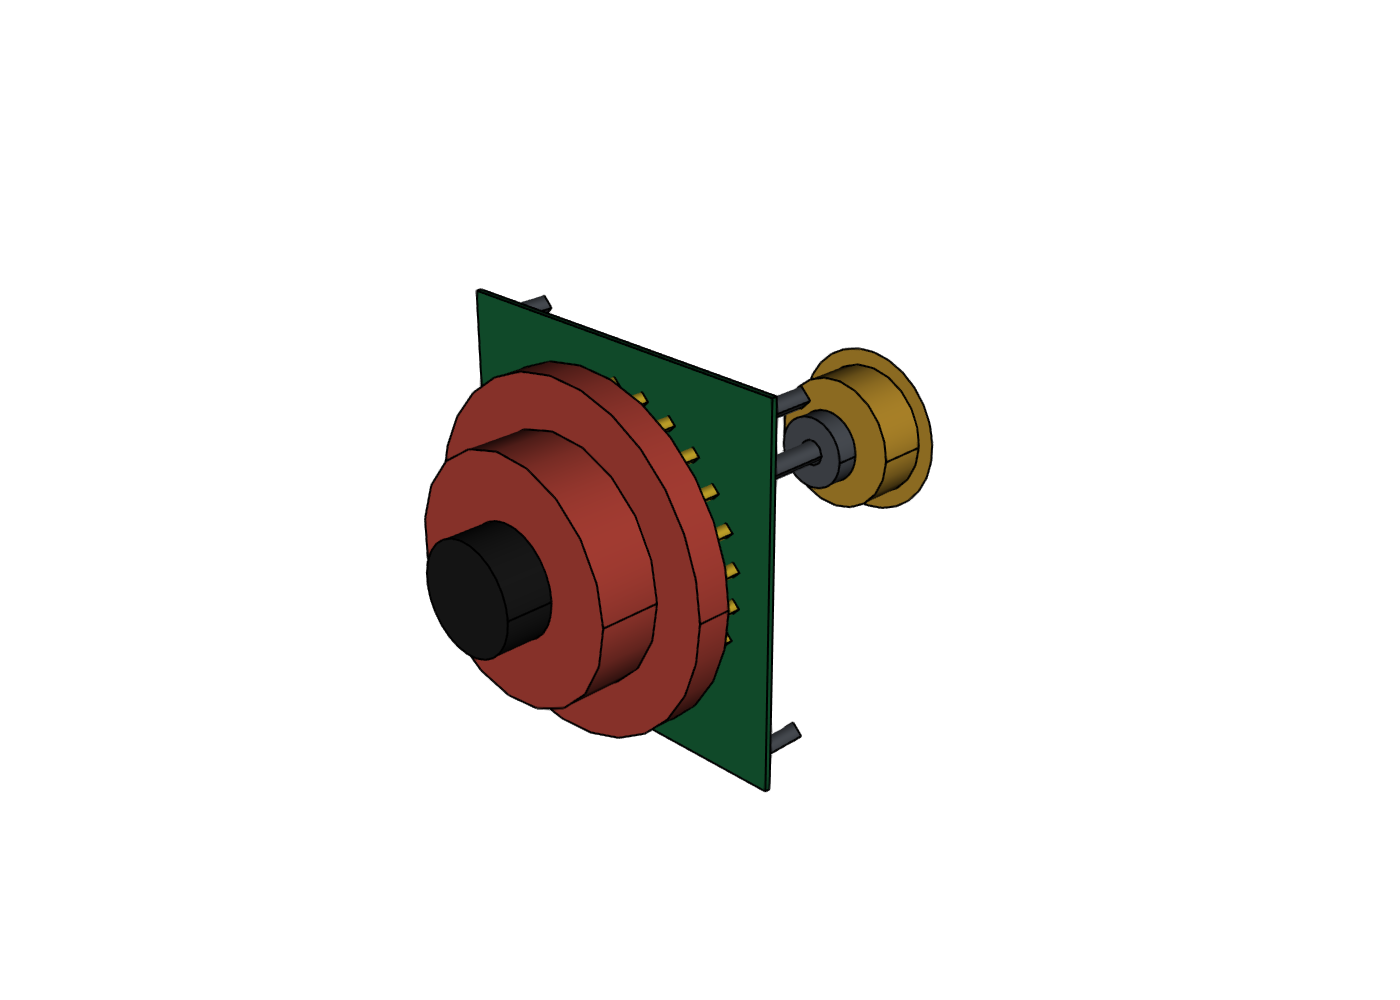
\includegraphics[width=0.48\linewidth]{../figures/generated/cad_station.png}\hfill
  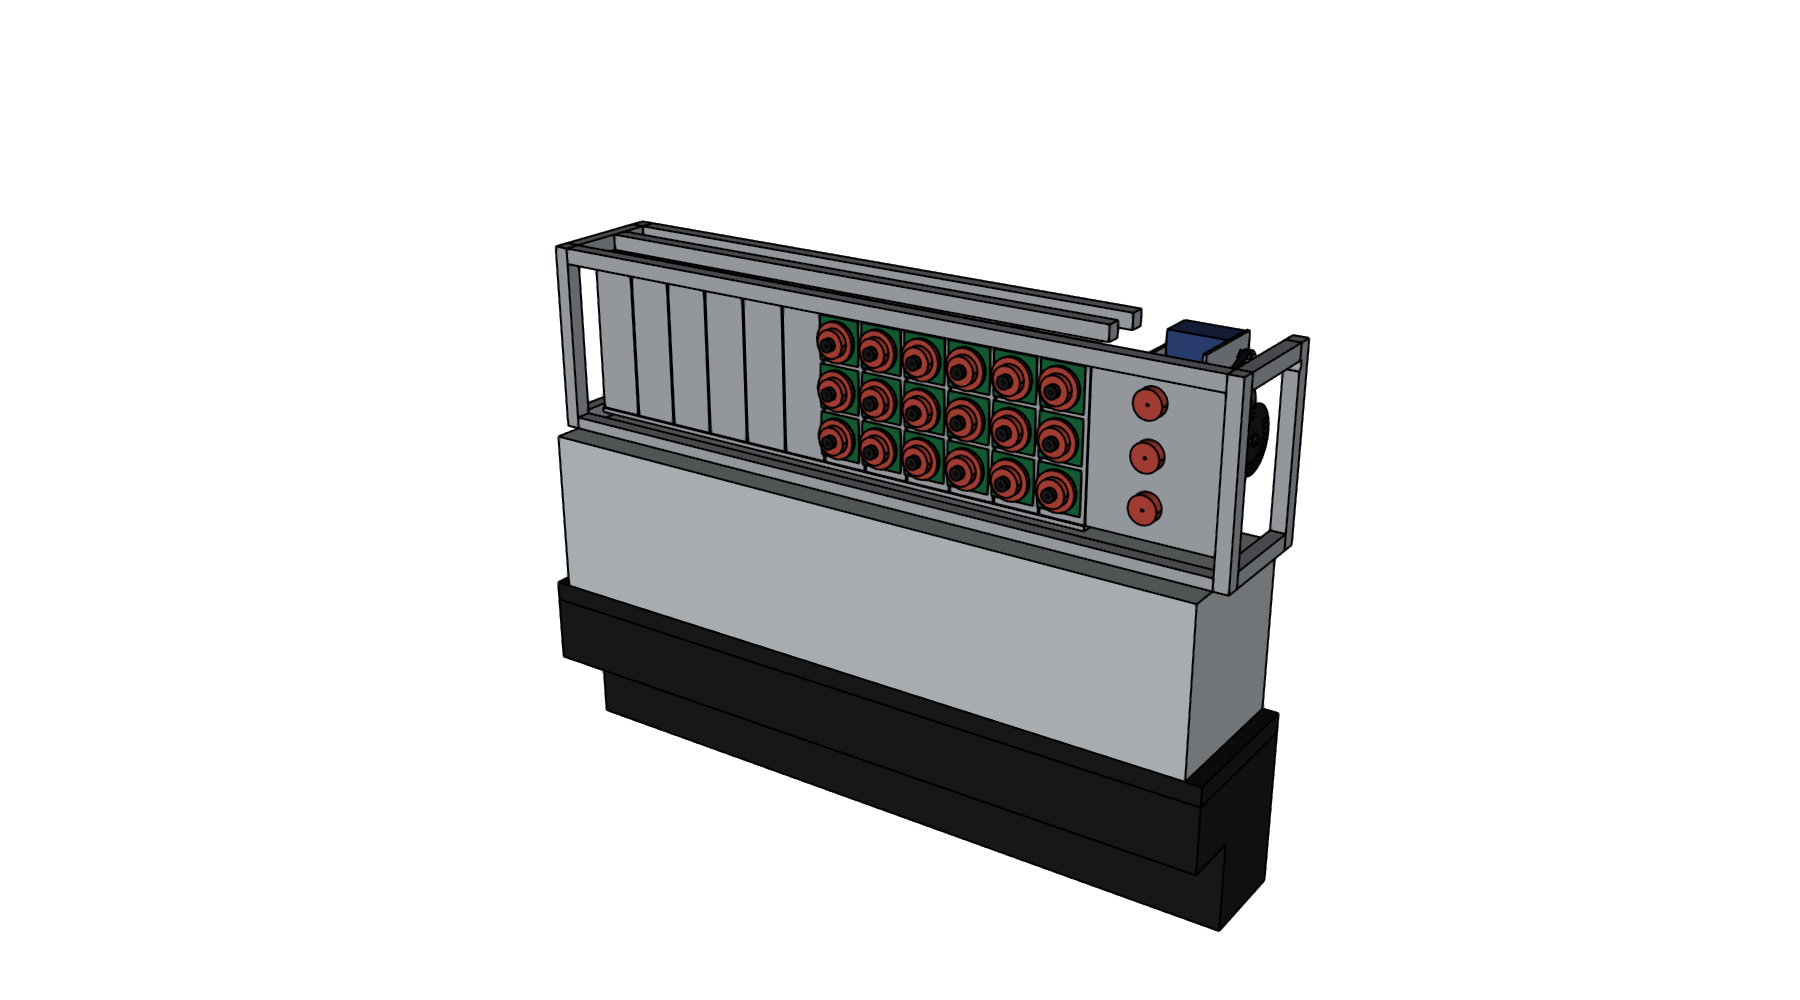
\includegraphics[width=0.48\linewidth]{../figures/generated/cad_iso.png}}{%
  \fbox{\parbox{0.9\linewidth}{\centering\footnotesize 그림 파일이 없다: \code{python hardware/gear/cad/render\_png.py}}}}
\caption{\code{render\_png.py}가 만든 그림. 왼쪽: 드럼 자리 하나(가운데 행)와 그 축의 쌓기. 오른쪽: 기계 전체(덮개를 뺀 것,
7--12번 자리에 열 모듈 여섯).}
\label{fig:gc-render}
\end{figure}

\section{정리}

\begin{itemize}
\item 기계 전체를 CadQuery 스크립트로 그린다. 숫자는 \code{params.py} 한 곳에만 있고, 숫자마다 출처(문서의 절)나
\code{(mod)}(모델링의 가정)가 붙는다. 다른 값에서 나오는 값은 계산식으로 적는다.
\item 부품은 단순한 입체의 더하기·빼기(CSG)로 만든다. 빼는 입체는 조금 넘치게 그린다. 반지름에 따라 깊어지는 V홈은 두
단면을 잇는 로프트로 판다.
\item 기계는 이름, 모양, 묶음, 역할을 가진 부품의 목록이다. 기어는 피치원으로 단순화하고, 무엇을 단순화했는지 적어 둔다.
\item \code{check.py}는 축간 거리, 패드 면, 외형, 덮개의 틈, 슬롯의 타이밍 여유를 재고, 경계 상자로 쌍을 고른 뒤 교집합
부피로 간섭을 잰다. 일부러 드럼을 1~mm 밀어 넣는 자기 시험으로 검사기 자신을 검사한다.
\item 모델이 문서의 치수 아홉 개(C1--C9)가 공간에서 닫히지 않음을 찾아냈다. 각각의 계산은 맞았지만 부품이 만나는 곳은 모델이
처음 보았다.
\item 슬롯 각도는 모터 스텝 단위로 \code{SLOT\_STEPS}에 한 번만 적고, 제어 보드의 펌웨어 모델과 시뮬레이션이 같은 파일을
읽는다.
\end{itemize}

\chapter{기어식 제어: 구동과 시간 신호}\label{ch:52-gear-control}

기어식 봄베의 판단은 테스트 레지스터의 릴레이가 한다. 기계 쪽에서 할 일은 둘이 남는다. 슬롯 원판의 광센서 신호를
24~V의 \code{STROBE}, \code{JUDGE}, \code{CLEAR}로 바꾸어 레지스터에 보내는 일, 그리고 모터를 돌리고 세우고 되돌리는 일이다.
이 장은 그 두 일을 맡는 구동부의 제어 보드(\code{hardware/gear/control-board})를 다룬다. 시간 규칙 L1--L9가 어디서
나왔는지는 \ref{ch:relay-timing}장에서, 슬롯 원판이 그 시각을 각도로 갖고 게이트가 L7과 L8을 지킨다는 것은
\ref{sec:t-gear}절에서 보았으므로 되풀이하지 않는다. 여기서는 그 규칙을 \emph{누가, 어떤 회로로} 지키는지,
그리고 그것을 어떻게 시뮬레이션으로 확인하는지를 본다.

\section{보드의 두 가지 일}\label{sec:gk-overview}

\Why 보드에는 마이크로컨트롤러(Raspberry Pi Pico)가 하나 있다. 그러면 \code{STROBE}도 Pico가 센서를 읽어 내보내면
간단할 것 같다. 그렇게 하지 않는다. 이유는 둘이다. 첫째, 프로젝트의 원칙(\code{design-brief.md} 1절)이 ``전자 장치는
구동과 신호 조건화만 하고 판정에는 관여하지 않는다''이다. 둘째, 펌웨어는 멈추거나, 늦거나, 틀릴 수 있다. 정지 판정의
시각이 펌웨어의 반복 주기나 버그에 달리면, 놓친 정지가 소프트웨어 버그 하나로 생길 수 있다. 그래서 일을 둘로 나눈다
(그림~\ref{fig:gk-block}).

\begin{enumerate}
\item \textbf{타이밍 경로}: 광센서 $\to$ RC 필터 $\to$ 슈미트 트리거 $\to$ 논리 게이트 $\to$ 고측 구동기 $\to$ 퓨즈 $\to$
커넥터 핀. 이 길에 \emph{펌웨어가 없다}. 시간은 슬롯이 정하고, 순서는 게이트가 지킨다.
\item \textbf{구동 제어}: Pico가 모터 구동기에 스텝 펄스를 주고, 정지·되돌림·재출발·\code{HOME}·\code{END}·위치 계수를
맡는다. 타이밍 경로에는 ``지금 내보내도 된다''는 허가 신호(\code{TXEN})와 ``원점 복귀 중''(\code{HOMING}) 두 선만 준다.
\end{enumerate}

\General 전자레인지의 문에는 스위치가 있어서 문이 열리면 마그네트론의 전원이 \emph{회로로} 끊긴다. 조작판의 마이크로컨트롤러가
문이 열린 것을 알아채고 끄기를 기다리지 않는다. 안전이나 정확성이 걸린 규칙을 소프트웨어 밖의 하드웨어에 두는 것은
흔한 설계 방식이다. 소프트웨어는 그 위에서 편의를 맡는다.

\begin{figure}[ht]
\centering
\begin{tikzpicture}[x=1cm,y=1cm,
    b/.style={blk,font=\footnotesize,minimum width=20mm},
    ar/.style={->,line width=0.7pt}]
  \node[b] (sen) at (0,2.2) {광센서 3\\(슬롯 원판)};
  \node[b] (rc) at (2.9,2.2) {RC + 74HC14};
  \node[blko,font=\footnotesize,minimum width=22mm] (g) at (6.0,2.2) {게이트\\(74HC08/32/02/74)};
  \node[b] (tbd) at (9.2,2.2) {TBD62783A\\+ 퓨즈};
  \node[blkn,font=\footnotesize,align=center] (jc) at (12.2,1.2) {\code{J\_CTRL}\\(테스트 레지스터,\\공통부)};
  \draw[ar] (sen) -- (rc); \draw[ar] (rc) -- node[above,font=\scriptsize] {\code{SLOT\_*}} (g);
  \draw[ar] (g) -- node[above,font=\scriptsize] {\code{*\_G}} (tbd);
  \draw[ar] (tbd) -| node[pos=0.25,above,font=\scriptsize] {\code{STROBE}, \code{JUDGE}, \code{CLEAR}} (jc.north);
  \node[blkb,font=\footnotesize,minimum width=22mm,minimum height=16mm] (pico) at (6.0,-0.2) {Pico\\(펌웨어)};
  \node[b] (pos) at (0,0.25) {광센서 6\\(위치 원판)};
  \draw[ar] (pos.east) -- node[above,font=\scriptsize] {T, I} (pos.east -| pico.west);
  \draw[ar,cblue] (pico) -- node[right,font=\scriptsize,text=cblue] {\code{TXEN}, \code{HOMING}} (g);
  \node[b] (opt) at (0,-0.75) {광커플러 입력};
  \draw[ar] (opt.east) -- (opt.east -| pico.west);
  \node[note,anchor=north] at (0,-1.15) {\code{RUN}, \code{STOP\_LATCH}, \code{HOME},\\\code{V48\_OK}, \code{SW\_OK}};
  \node[b] (drv) at (9.2,-0.2) {모터 구동기\\(폐루프 스테퍼)};
  \draw[ar] (pico) -- node[above,font=\scriptsize] {\code{PUL}/\code{DIR}/\code{ENA}} (drv);
  \node[b] (sr) at (9.2,-1.9) {74HC595 + 구동기};
  \draw[ar] (pico.south) |- (sr.west);
  \draw[ar] (sr.east) -| node[pos=0.25,below,font=\scriptsize,align=center] {\code{STOPPED}, \code{AT\_HOME},\\\code{END}, \code{POS0--14}} (jc.south);
  \begin{pgfonlayer}{background}
    \fill[corangebg!50] (-1.2,1.55) rectangle (10.4,2.9);
  \end{pgfonlayer}
  \node[font=\scriptsize,text=corange,anchor=south west] at (-1.2,2.9) {펌웨어가 없는 길};
\end{tikzpicture}
\caption{기어식 제어 보드. 위쪽 띠가 타이밍 경로이고, Pico는 그 길에 허가 신호 두 개만 준다. 릴레이는 하나도 없다.}
\label{fig:gk-block}
\end{figure}

\Ours 보드의 부품은 216개이고 그중 집적회로가 19개다. \code{RUN}이나 \code{HOME} 같은 받는 신호는 모두
2.2~k$\Omega$ 저항과 \term{광커플러}{optocoupler}를 지난다. 광커플러는 LED와 빛을 받는 트랜지스터를 한 칩에 넣은 것으로,
24~V 쪽 신호가 LED를 켜면 3.3~V 쪽 트랜지스터가 켜진다. 두 쪽이 빛으로만 이어지므로 24~V의 잡음이나 사고 전압이 Pico로
들어오지 않는다. 내는 신호는 \term{고측 구동기}{high-side driver} TBD62783A가 +24~V를 핀에 이어 주고, 핀마다 자동 복귀
퓨즈가 단락을 막는다.

\paragraph{느린 에지를 깨끗하게.} 광센서의 출력은 슬롯 가장자리가 천천히 지나가는 동안 천천히 변하고 잡음이 섞인다.
문턱 하나로 0과 1을 가르면 문턱 근처에서 여러 번 오르내릴 수 있다. 그래서 RC 필터(약 5~$\mu$s)로 잔 떨림을 깎은 뒤
\term{슈미트 트리거}{Schmitt trigger}(74HC14)에 넣는다. 슈미트 트리거는 오를 때의 문턱(이 시뮬레이션은 1.9~V로 둔다)과
내릴 때의 문턱(1.0~V)이 다르다. 한 번 넘어가면 반대쪽 문턱까지 돌아와야 다시 넘어가므로 문턱 근처의 떨림이 출력에
나타나지 않는다. 난방 온도 조절기가 20°C에서 켜고 22°C에서 끄는 것도 같은 이유다. 하나의 온도로 켜고 끄면 보일러가
쉴 새 없이 켜졌다 꺼진다.

\section{스테퍼 모터와 가감속}\label{sec:gk-stepper}

\Why \term{스테퍼 모터}{stepper motor}는 펄스 하나에 정해진 각도만큼 돈다. 펄스의 수가 곧 위치이고 펄스의 빠르기가 곧
속도이므로, 위치를 세기 쉽고 원하는 자리에 세우기 쉽다. 약점은 \term{탈조}{stall, lost step}다. 펄스를 너무 갑자기
빠르게 주면 회전자가 관성 때문에 따라오지 못하고 미끄러져, 펄스 수와 실제 위치가 어긋난다. 이 기계의 모터는 엔코더가
달린 \term{폐루프}{closed-loop} 스테퍼여서 어긋남을 스스로 바로잡지만, 그래도 정지 상태에서 곧바로 최고 속도의
펄스를 주면 따라오지 못한다. 그래서 속도를 천천히 올리고(\term{가속}{acceleration}) 천천히 내려야(감속) 한다.

\General 자동차는 정지 상태에서 시속 100~km로 순간 이동하지 않는다. 3D 프린터의 설정에 ``가속도'' 항목이 있는 것도 같다.
흔한 방법은 \term{사다리꼴 속도}{trapezoidal profile}다. 일정한 가속도로 오르고, 일정한 속도로 가고, 일정한 감속도로
내린다(그림~\ref{fig:gk-ramp}). 언제 감속을 시작할지는 제동 거리로 정한다. 속도 $v$에서 감속도 $a$로 서는 데 드는 거리는
$v^2 / (2a)$이므로, 남은 거리가 $d$이면 지금 낼 수 있는 가장 빠른 속도는 $\sqrt{2ad}$다. 이보다 빠르면 제때 서지 못한다.

\begin{figure}[ht]
\centering
\begin{tikzpicture}[x=1cm,y=1cm]
  \draw[->] (0,0) -- (11,0) node[right,font=\scriptsize] {시간};
  \draw[->] (0,0) -- (0,2.4) node[above,font=\scriptsize] {속도 (스텝/s)};
  \draw[cblue,line width=1.2pt] (0,0) -- (1.6,1.8) -- (8.0,1.8) -- (9.1,0);
  \draw[dashed,cgray] (0,1.8) node[left,font=\scriptsize,text=black] {10,400} -- (1.6,1.8);
  \node[note,anchor=south] at (0.8,1.9) {가속\\$8 \times 10^5$/s$^2$};
  \node[note,anchor=south] at (4.8,1.9) {60~rpm = 26위치/s};
  \node[note,anchor=south west] at (8.4,1.0) {정지 감속\\$1.2 \times 10^6$/s$^2$};
  \draw[corange,dashed,domain=0:1.1,samples=20] plot ({9.1-\x},{1.8*sqrt(\x/1.1)});
  \node[note,anchor=north,text=corange] at (8.2,-0.15) {$v \le \sqrt{2a \cdot \text{남은 거리}}$};
\end{tikzpicture}
\caption{사다리꼴 속도. 감속 구간의 곡선(주황 점선)은 ``남은 거리에서 설 수 있는 가장 빠른 속도''다. 위치 이동 함수는 매
순간 이 값과 최고 속도 가운데 작은 쪽을 목표로 삼는다. 가속도 값은 추정이며 기어식 시제품(G.2)에서 정한다.}
\label{fig:gk-ramp}
\end{figure}

\Ours 구동기는 모터 한 바퀴를 2,600펄스로 나누도록 설정한다. 4:1 벨트와 26위치를 거치면 한 위치가 400스텝이고, 60~rpm은
초당 26위치, 곧 10,400~pps(초당 펄스)다(\ref{sec:gc-slotsteps}절). 구동기 쪽에는 자체 가감속이 없으므로 Pico가 펄스의
빠르기를 조금씩 바꾸어 사다리꼴을 만든다. 구동기를 펄스/방향(step/dir) 방식으로 고른 이유는 되돌림 때문이다. ``돌아라/서라''만
받는 구동기로는 정지한 위치로 거꾸로 몇 스텝 돌아가는 일을 할 수 없다.

펌웨어의 명세는 실행할 수 있는 Python 파일 \code{firmware\_model.py}다. Pico에 올릴 MicroPython은 이 파일을 옮겨 쓴다.
위치로 가는 함수는 앞의 규칙을 그대로 쓴다.

\begin{lstlisting}[language=Python,caption={\code{firmware\_model.py}: 목표 스텝까지 사다리꼴로 간다(발췌).},label={lst:gk-goto}]
    def _goto(self, target: int, vmax: float, a: float, dt: float):
        """move to the absolute step target with a trapezoid profile; returns (steps, arrived)"""
        rem = target - self.s
        if rem == 0 and abs(self.v) < 1.0:
            self.v = 0.0
            return 0, True
        d = 1 if rem > 0 else -1
        vd = d * min(vmax, math.sqrt(2.0 * a * max(abs(rem) - 0.5, 0.0)))
        n = self._motion(vd, a, dt)
        if (target - self.s) * d < 0:          # never overshoot (closed-loop drive: exact step count)
            ...
\end{lstlisting}

\code{vd}가 ``이번 순간의 목표 속도''다. 남은 거리가 많으면 \code{vmax}, 적으면 $\sqrt{2a \cdot \text{남은 거리}}$다.
\code{\_motion}은 현재 속도를 한 틱에 $a \cdot dt$ 이상 바꾸지 않으면서 \code{vd}로 다가가고, 그 틱에 낼 스텝 수를 돌려준다.
예를 들어 정격 속도 10,400~pps에서 정지 감속 $1.2 \times 10^6$~스텝/s$^2$로 서면 $10400^2 / (2 \times 1.2 \times 10^6) \approx
45$스텝을 더 간다. 슬롯 원판의 한 위치가 400스텝이므로 정지 신호를 받고 한 위치의 9분의 1 안에 선다.

여기에는 \ref{sec:t-bounds}절의 ``느려지면 늘 안전하다''가 깔려 있다. L1--L6은 모두 시간의 하한이고 슬롯이 각도로
시각을 정하므로, 가속이나 감속 중에 모터가 느려지면 모든 구간이 시간으로 길어진다. 위험한 것은 빨라지는 쪽뿐이고,
램프는 10,400~pps를 넘지 않게 되어 있다.

\section{펌웨어가 없는 길: 게이트 셋과 플립플롭 둘}\label{sec:gk-gates}

\Why 슬롯이 센서를 지나는 동안 신호를 그대로 핀에 내보내기만 하면 대부분의 규칙(L1--L6)은 슬롯의 각도가 지킨다
(\ref{sec:t-gear}절). 남는 것은 순서에 관한 두 규칙과 ``내보내지 말아야 할 때''다.

\begin{itemize}
\item \textbf{L7}: \code{STROBE}를 낸 위치에는 \code{JUDGE}와 \code{CLEAR}를 반드시 낸다. 펌웨어가 주기 한가운데서 허가를
거두어도(예를 들어 되돌아가려고) 시작한 주기는 끝나야 한다.
\item \textbf{L8}: 전원 투입, \code{HOME}, 정지 해제 뒤에는 \code{STROBE}를 한 번 내기 전에 \code{JUDGE}를 내지 않는다. 비어 있는
레지스터를 판정하면 곧 정지(거짓 정지)이기 때문이다.
\item \code{HOME} 동작 중, 거꾸로 되돌아가는 동안, 비상 정지 중에는 내보내지 않는다(\code{TXEN}).
\end{itemize}

이 셋을 논리식 몇 줄과 \term{D 플립플롭}{D flip-flop} 두 개로 만든다. \ref{ch:sync}장의 플립플롭은 클럭의 오르는 에지에서
입력 D를 받아 들고 있는 1비트 기억이었다. 74HC74는 여기에 클럭과 상관없이 출력을 1로 만드는 \emph{세트} 입력과 0으로
만드는 \emph{리셋} 입력이 따로 달린 칩이다.

\Ours 회로는 그림~\ref{fig:gk-gates}이고 식은 이렇다(\code{README.md} 1.1절). 코드~\ref{lst:t-gate}와 같은 식을
여기서는 회로와 시간으로 풀어 본다.
\begin{lstlisting}[numbers=none,caption={타이밍 경로의 논리.},label={lst:gk-eq}]
  STROBE_G = SLOT_S & TXE
  CLEAR_G  = SLOT_C & TXE
  JUDGE_G  = SLOT_J & SEEN & TXE
  TXE      = TXEN | CYC
  CYC  : set while STROBE_G is high, cleared by the fall of CLEAR_G; reset by POR | HOMING      (L7)
  SEEN : set by the rise of STROBE_G, cleared by POR | HOMING | fall of STOP_LATCH            (L8)
\end{lstlisting}

\begin{figure}[ht]
\centering
\begin{tikzpicture}[x=1cm,y=1cm,
    lb/.style={font=\scriptsize\ttfamily},
    ff/.style={draw,fill=cyellowbg,minimum width=30mm,minimum height=16mm,align=left,font=\scriptsize,inner sep=3pt}]
  % OR
  \node[or gate US,gate] (or1) at (1.2,0) {};
  \draw (or1.input 1) -- ++(-0.5,0) node[left,lb] {TXEN};
  \draw (or1.input 2) -- ++(-0.5,0) node[left,lb] {CYC};
  \draw (or1.output) -- ++(0.4,0) node[right,lb] {TXE};
  % ANDs
  \node[and gate US,gate] (a1) at (5.4,1.4) {};
  \draw (a1.input 1) -- ++(-0.5,0) node[left,lb] {SLOT\_S};
  \draw (a1.input 2) -- ++(-0.5,0) node[left,lb] {TXE};
  \draw (a1.output) -- ++(0.4,0) node[right,lb] {STROBE\_G};
  \node[and gate US,gate] (a2) at (5.4,0.0) {};
  \draw (a2.input 1) -- ++(-0.5,0) node[left,lb] {SLOT\_C};
  \draw (a2.input 2) -- ++(-0.5,0) node[left,lb] {TXE};
  \draw (a2.output) -- ++(0.4,0) node[right,lb] {CLEAR\_G};
  \node[and gate US,gate] (a3) at (4.6,-1.5) {};
  \draw (a3.input 1) -- ++(-0.5,0) node[left,lb] {SLOT\_J};
  \draw (a3.input 2) -- ++(-0.5,0) node[left,lb] {SEEN};
  \node[and gate US,gate] (a4) at (7.2,-1.9) {};
  \draw (a3.output) -- ++(0.2,0) |- (a4.input 1);
  \draw (a4.input 2) -- ++(-0.5,0) node[left,lb] {TXE};
  \draw (a4.output) -- ++(0.4,0) node[right,lb] {JUDGE\_G};
  % flip-flops
  \node[ff] (seen) at (12.2,1.0) {\textbf{SEEN} (74HC74 1)\\D = 1, 클럭 = \code{STROBE\_G} $\uparrow$\\리셋 = POR $\vee$ HOMING\\\phantom{리셋 = }$\vee$ \code{STOP\_LATCH} $\downarrow$ 펄스};
  \node[ff] (cyc) at (12.2,-1.2) {\textbf{CYC} (74HC74 2)\\세트 = \code{STROBE\_G}가 높은 동안\\D = 0, 클럭 = \code{CLEAR\_G} $\downarrow$\\리셋 = POR $\vee$ HOMING};
  \node[note,anchor=north] at (6.0,-2.4) {같은 이름의 선끼리 이어져 있다(회로도의 전역 레이블과 같다)};
\end{tikzpicture}
\caption{타이밍 경로의 게이트(74HC08 넷, 74HC32 하나)와 플립플롭 둘. 세 출력 \code{*\_G}가 TBD62783A와 퓨즈를 거쳐
\code{J\_CTRL}의 핀 1(\code{STROBE}), 34(\code{JUDGE}), 35(\code{CLEAR})로 나간다.}
\label{fig:gk-gates}
\end{figure}

\paragraph{CYC: 시작한 주기는 끝낸다 (L7).} \code{CYC}는 ``지금 주기 안에 있다''를 기억한다. \code{STROBE\_G}가 높은 동안 세트
입력이 걸려 1이 되고, \code{CLEAR\_G}가 내려가는 순간 클럭이 D = 0을 받아 0이 된다. \code{TXE}는 \code{TXEN}과 \code{CYC}의
OR이므로, 주기 안에서는 Pico가 \code{TXEN}을 내려도 \code{TXE}가 1로 남는다. 그림~\ref{fig:gk-cyc}가 그 경우다. \code{STROBE}
직후에 \code{TXEN}이 내려가도 그 주기의 \code{JUDGE}와 \code{CLEAR}는 나가고, \code{CLEAR}가 끝나 \code{CYC}가 지워진 뒤 다음
\code{STROBE} 슬롯은 막힌다.

\begin{figure}[ht]
\centering
\begin{tikztimingtable}[timing/slope=0.05,timing/coldist=4pt,xscale=0.29,yscale=1.1,semithick]
  \code{SLOT\_S}   & .5L 7H 31L 7H .5L \\
  \code{SLOT\_J}   & 11.5L 8H 26.5L \\
  \code{SLOT\_C}   & 21.5L 13H 11.5L \\
  \code{TXEN}      & 10H 36L \\
  \code{CYC}       & .5L 34H 11.5L \\
  \code{TXE}       & 34.5H 11.5L \\
  \code{SEEN}      & .5L 45.5H \\
  \code{STROBE\_G} & .5L 7H 38.5L \\
  \code{JUDGE\_G}  & 11.5L 8H 26.5L \\
  \code{CLEAR\_G}  & 21.5L 13H 11.5L \\
\extracode
  \begin{pgfonlayer}{background}
    \fill[credbg] (10,1.0) rectangle (10.4,-6.6);
    \fill[cgreenbg] (38.5,-14.2) rectangle (45.5,-12.8);
  \end{pgfonlayer}
  \node[note,text=cred,anchor=south] at (10.2,1.0) {Pico가 허가를 거둠};
  \node[note,text=cgreen,anchor=west] at (46.2,-13.5) {막힘};
\end{tikztimingtable}
\caption{L7을 지키는 \code{CYC}. 가로는 시간(한 칸 약 1~ms, 60~rpm). \code{TXEN}이 주기 한가운데서 내려가도 \code{CYC}가
\code{TXE}를 붙들어 \code{JUDGE}와 \code{CLEAR}가 나간다. \code{CLEAR\_G}가 내려가며 \code{CYC}가 지워진 뒤에는 다음 \code{STROBE}
슬롯이 와도 \code{STROBE\_G}가 나가지 않는다.}
\label{fig:gk-cyc}
\end{figure}

\paragraph{SEEN: STROBE 없이 JUDGE 없다 (L8).} \code{SEEN}은 ``이번 출발 뒤로 \code{STROBE}를 한 번이라도 냈는가''를 기억한다.
D가 늘 1이고 클럭이 \code{STROBE\_G}이므로 \code{STROBE}가 처음 오를 때 1이 되고, 지워지기 전까지 그대로다. \code{JUDGE\_G}는
\code{SEEN}이 1일 때만 나간다. 지우는 조건은 전원 투입(POR: 전원이 들어온 뒤 약 10~ms 동안 내는 리셋), \code{HOMING},
그리고 \code{STOP\_LATCH}가 \emph{내려가는 순간}이다.

``내려가는 순간''이 설계의 요점이다. \code{STOP\_LATCH}는 레지스터의 정지 릴레이가 붙으면 오르고 해제 버튼을 누르면 내린다.
\code{STOP\_LATCH}가 \emph{높은 동안} 내내 \code{SEEN}을 지우도록(레벨로) 하면 문제가 생긴다. 정지는 \code{JUDGE} 도중에
판정되므로 \code{STOP\_LATCH}가 \code{JUDGE} 한가운데서 오르고, 그 순간 \code{SEEN}이 지워져 \code{JUDGE}가 잘린다. 정지
릴레이가 자기 유지에 들기 전에 판정 경로가 열려 버릴 수 있다. 그래서 해제 때에만, 곧 \code{STOP\_LATCH}가 내려가는
에지에서만 지운다.

에지는 RC 지연으로 만든다. $\overline{\text{STOP\_LATCH}}$를 47~k$\Omega$과 10~nF(약 0.5~ms)로 늦춘 것을 뒤집어, 늦추지
않은 것과 AND한다. $\overline{\text{STOP\_LATCH}}$가 오른 직후 0.5~ms 동안만 두 입력이 모두 1이므로, 그 AND가 짧은 펄스
하나를 낸다. 계단의 ``지금''과 ``조금 전''을 비교해 바뀐 순간만 잡는 \term{에지 검출기}{edge detector}다.

\paragraph{부팅 중에도.} Pico가 켜지는 동안 핀은 아직 프로그램을 따르지 않는다. 그래서 \code{TXEN}에는 풀다운 저항(기본 0,
내보내지 않음), \code{HOMING}에는 풀업 저항(기본 1, \code{SEEN}과 \code{CYC}를 지운 채)을 단다. 펌웨어가 아무것도 하지
않아도 보드는 안전한 쪽에 있다.

\section{서고, 되돌아가고, 다시 출발한다}\label{sec:gk-stop}

\Why 레지스터가 정지를 판정하면(\code{STOP\_LATCH}가 오름) 모터를 세워야 한다. 그런데 아무 데나 서면 안 된다. 그 위치의
주기(\code{STROBE}--\code{JUDGE}--\code{CLEAR})는 끝까지 마쳐야 하고(L7), 다음 위치의 \code{STROBE} 슬롯 안에 서면 재출발할 때
그 \code{STROBE}가 반쪽만 나간다. 설 수 있는 곳은 \code{CLEAR} 슬롯이 끝난 뒤부터 다음 \code{STROBE} 슬롯이 시작하기 전까지,
한 위치 400스텝 가운데 330--374스텝, 44스텝(1.32°)뿐이다. 이것을 \term{정지 자리}{stop zone}라 한다(그림~\ref{fig:gk-zone}).

\General 엘리베이터는 층에 가까워지면 감속하고, 마지막에는 아주 천천히 기어 가서 바닥 높이를 맞춘다. 빠르게 가다가 정확한
높이에 한 번에 서려고 하지 않는다. 지나쳤으면 조금 되돌아간다.

\begin{figure}[ht]
\centering
\begin{tikzpicture}[x=0.028cm,y=1cm]
  \draw[->] (-60,0) -- (470,0) node[right,font=\scriptsize] {스텝};
  \foreach \t in {0,100,200,300,400} \draw (\t,0.06) -- (\t,-0.06) node[below,font=\tiny] {\t};
  \fill[cbluebg] (-26,0.2) rectangle (47,0.5); \node[font=\tiny] at (10,0.35) {\code{STROBE}};
  \fill[cgreenbg] (89,0.2) rectangle (173,0.5); \node[font=\tiny] at (131,0.35) {\code{JUDGE}};
  \fill[corangebg] (194,0.2) rectangle (330,0.5); \node[font=\tiny] at (262,0.35) {\code{CLEAR}};
  \fill[cbluebg] (374,0.2) rectangle (447,0.5); \node[font=\tiny] at (410,0.35) {다음 \code{STROBE}};
  \fill[credbg] (330,0.55) rectangle (374,0.85);
  \node[font=\tiny,text=cred,anchor=south] at (352,0.85) {정지 자리 44};
  \draw[cred,line width=1.2pt] (340,0.1) -- (340,0.95);
  \node[font=\tiny,text=cred,anchor=south] at (300,1.2) {목표 = \code{CLEAR} 끝 + 10};
  \draw[->,cred] (310,1.2) -- (338,0.97);
  \draw[cgray,dashed] (280,-0.3) -- (280,0.55);
  \node[note,anchor=north] at (250,-0.3) {\code{POS} 경계 +280};
  \draw[cred,dashed] (350,-0.3) -- (350,0.55);
  \node[note,anchor=north west,text=cred] at (335,-0.3) {먼 쪽이 최악일 때 +350:\\목표 양쪽에 약 10스텝};
\end{tikzpicture}
\caption{한 위치(400스텝, 0은 \code{STROBE} 접점의 시작) 안의 슬롯과 정지 자리. 되돌림 목표는 펌웨어가 \emph{센서에서 직접
잰} \code{CLEAR}의 끝에서 10스텝 뒤다. 먼 쪽 가장자리(다음 \code{STROBE} 슬롯의 시작)는 \code{STROBE} 보정에 따라 최악 약
20스텝까지 당겨지므로 목표 양쪽에 약 10스텝씩 남는다.}
\label{fig:gk-zone}
\end{figure}

\Ours 펌웨어는 \term{상태 기계}{state machine}(\ref{sec:fsm}절)다. 상태는 \code{REST}, \code{RUN}, \code{STOPDEC},
\code{CREEPOUT}, \code{RET}과 \code{HOME}에 쓰는 몇 개다(그림~\ref{fig:gk-states}). 정지는 이렇게 흘러간다.

\begin{enumerate}
\item \code{RUN}에서 \code{STOP\_LATCH}가 오르면 \code{STOPDEC}로 가서 정지 감속으로 선다. \code{STOP\_LATCH}는 \code{JUDGE}
슬롯이 오른 뒤 5--9~ms에 오르고 축은 약 45스텝 더 가므로, 보통 \code{CLEAR} 슬롯 안에서 선다.
\item \code{CREEPOUT}: 천천히(2,000~pps) 앞으로 기어 가며 그 주기의 \code{CLEAR} 슬롯이 \emph{끝나는 에지}를 기다린다. 센서
인터럽트가 그 순간의 스텝 수를 \code{s\_clear\_end}에 적는다.
\item 목표를 \code{s\_clear\_end + 10}으로 잡는다. 목표가 지금보다 뒤에 있으면(감속이 약해 지나쳤으면) \code{TXEN}을 내리고
되돌아간다. 거꾸로 지나가는 슬롯에서 신호가 나가면 안 되기 때문이다(결정 0003 4.4절).
\item \code{RET}: 목표까지 가서 \code{REST}. \code{STOPPED} = 1, 위치 버스 \code{POS}에 정지한 위치를 보인다.
\end{enumerate}

\begin{lstlisting}[language=Python,caption={\code{firmware\_model.py}: \code{CREEPOUT} 상태(발췌).},label={lst:gk-creep}]
        elif st == "CREEPOUT":
            ...
            if self.stop_kind == "latch":
                if self.s_clear_end is None:
                    n = self._motion(p.v_creep, p.a_creep, dt)       # forward until CLEAR has ended
                else:
                    self.ret_target = self.s_clear_end + p.ret_offset
                    if "no_txen_return" not in self.mut and self.ret_target < self.s:
                        self.txen = False                              # reverse: no timing outputs (4.4 (2))
                    self.state = "RET"
            else:
                if slot_any or self.in_cycle:                     # operator stop / END: stand between two cycles
                    n = self._motion(p.v_creep, p.a_creep, dt)
                else:
                    n = self._motion(0.0, p.a_creep, dt)
                    if self.v == 0.0:
                        self._rest_after_stop()
\end{lstlisting}

\code{"no\_txen\_return" not in self.mut} 같은 조건은 음성 시험용이다(\ref{sec:gk-verify}절). 검증기가 일부러 이 규칙을 빼 본
펌웨어를 돌려, 빼면 반드시 실패가 나오는지를 확인한다.

\paragraph{왜 각도가 아니라 에지인가.} ``정지 자리의 가운데(352스텝)에 선다''로 정할 수도 있다. 그러나 그 352는 설계 각도이고,
실제 원판의 가공 오차와 센서 브래킷의 오차가 거기에 그대로 얹힌다. 목표를 \emph{센서가 잰} \code{CLEAR}의 끝에서 세면
가까운 쪽 가장자리의 오차는 상쇄된다. 남는 것은 먼 쪽이다. 먼 쪽은 따로 도는 \code{STROBE} 센서 브래킷이 정하는데, 물린
레지스터의 \code{STROBE} 릴레이가 가장 느리면 보정이 슬롯을 1.5~ms 앞당기고, 보정의 흩어짐과 \code{CLEAR} 센서의 0.1°를 더하면
정지 자리가 최악 약 20스텝으로 준다(계산). 그래서 목표는 +10이다. 처음에는 +20이었는데, 그러면 최악의 경우 목표가 다음
\code{STROBE} 슬롯 안에 들 수 있었다(\code{README.md} 6절 3번). 폐루프 스테퍼의 정지 정확도 $\pm$1--2스텝(추정)이 양쪽 10스텝
안에 들어간다.

\begin{figure}[ht]
\centering
\begin{tikzpicture}[x=1cm,y=1cm,
    s/.style={draw,rounded corners=3pt,fill=cbluebg,draw=cblue,minimum width=19mm,minimum height=7mm,font=\scriptsize\ttfamily},
    h/.style={s,fill=cgreenbg,draw=cgreen},
    lab/.style={font=\tiny,fill=white,inner sep=1pt,align=center},
    ar/.style={->,line width=0.6pt}]
  \node[s,fill=cyellowbg,draw=corange] (rest) at (0,0) {REST};
  \node[s] (run) at (3.8,0) {RUN};
  \node[s] (dec) at (7.6,0) {STOPDEC};
  \node[s] (crp) at (7.6,-2.0) {CREEPOUT};
  \node[s] (ret) at (3.8,-2.0) {RET};
  \node[h] (hmv) at (-3.4,-1.0) {HMOVE};
  \node[h,align=center] (hsr) at (-3.4,-2.9) {HSEARCH\\{\tiny(HBACK, HDEC, HGO)}};
  \node[h] (hfl) at (0,-2.9) {HFLUSH};
  \draw[ar] (rest) -- node[lab,above] {\code{RUN} $\wedge$ \code{RUNARM}} (run);
  \draw[ar] (run) -- node[lab,above] {\code{STOP\_LATCH}$\uparrow$,\\\code{RUN}$\downarrow$, \code{END}} (dec);
  \draw[ar] (dec) -- node[lab,right] {속도 0} (crp);
  \draw[ar] (crp) -- node[lab,above] {\code{CLEAR} 끝을 잡음} (ret);
  \draw[ar] (ret) -- node[lab,above left] {도착: \code{STOPPED}} (rest);
  \draw[ar] (crp.south) -- (7.6,-3.8) -- node[lab,below] {조작 정지·\code{END}: 주기 사이에서 섬} (1.6,-3.8) -- (1.6,-0.35) -- (rest.south east);
  \draw[ar] (rest.west) -- node[lab,above] {\code{HOME}, 계수 맞음} (hmv.north east);
  \draw[ar] (rest.south west) -- node[lab,pos=0.6,left] {\code{HOME},\\계수 모름} (hsr.north east);
  \draw[ar] (hmv.south east) -- (hfl.west);
  \draw[ar] (hsr) -- node[lab,below] {원점 표시} (hfl);
  \draw[ar] (hfl) -- node[lab,right] {\code{AT\_HOME}} (rest);
\end{tikzpicture}
\caption{펌웨어의 상태(\code{firmware\_model.py}). 파란 상태가 운전과 정지, 초록 상태가 \code{HOME}이다.}
\label{fig:gk-states}
\end{figure}

\paragraph{재출발.} 해제 버튼을 누르면 레지스터가 \code{STOP\_LATCH}를 내리고 \code{RUN}을 올린다. 펌웨어는 \code{REST}에서
\code{RUN}으로 가고 \code{TXEN}을 올린다. 축은 정지 자리에 있으므로 처음 만나는 것은 \emph{다음} 위치의 \code{STROBE} 슬롯이다.
정지한 위치 $n$은 다시 시험하지 않고 $n+1$부터 이어 간다. 그리고 \code{STOP\_LATCH}가 내려간 에지가 \code{SEEN}을 지웠으므로,
그 \code{STROBE}가 오기 전에는 \code{JUDGE}가 나가지 않는다.

\paragraph{조작 정지.} 관람객이 시작 스위치를 끄면(\code{RUN}만 내려감) 판정과 상관없이 선다. 이때는 되돌아갈 위치가 없으므로
감속한 뒤 ``슬롯 밖이고 주기가 끝난 곳''까지 기어 가서 선다. 레지스터에 반쯤 끝난 주기를 남기지 않기 위해서다.

\section{\texorpdfstring{\code{HOME}}{HOME}: 처음 자리로}\label{sec:gk-home}

\Why \code{HOME}은 세 드럼을 모두 첫 위치로 돌리고 기계를 원위치에 세우는 동작이다. 관람객이 드럼을 바꾸기 전에 누르고
(\ref{sec:gm-brake}절), 비상 정지 뒤에도 반드시 거친다. 할 일은 세 가지다. 원위치를 \emph{하나로} 찾는 것, 가는 동안 타이밍
신호를 내지 않는 것, 그리고 끝에 레지스터를 깨끗이 비워 두는 것이다.

\Ours \code{HOME} 단추를 100~ms 이상 누르고 있고 \code{RUN}과 \code{STOP\_LATCH}가 모두 0이면 시작한다. 펌웨어는
\code{HOMING} = 1, \code{TXEN} = 0으로 둔다.

\begin{itemize}
\item \textbf{계수기가 맞으면}(위치 원판의 계수를 믿을 수 있으면) 짧은 쪽 방향으로 간다. 한 바퀴가 17,576위치이므로 많아야
그 절반인 8,788위치다. 거꾸로 가는 동안에도 \code{TXEN} = 0이므로 신호가 나가지 않는다.
\item \textbf{계수기를 모르면} 앞으로(\code{RUN}의 두 배 속도) 찾아간다. 원위치의 표시는 ``세 원점 센서가 모두 높은 동안
\code{STROBE} 슬롯이 오르는 곳''이다. 세 원점 센서만으로는 안 된다. 주기 축의 0번째 회전 안에서 빠른 드럼이 글자 A를 보이는
칸이 $k = 0$과 빈 칸 $k = 26$ 둘이기 때문이다(\ref{sec:gm-posdisc}절). 0번째 회전 안에서 찾기 시작했으면 먼저 그 밖으로
물러난 뒤 찾는다.
\end{itemize}

\paragraph{끝의 \code{CLEAR} 한 번(\code{HFLUSH}).} 비상 정지는 위치 주기의 어디서나 전원을 끊는다. \code{STROBE} 뒤, \code{CLEAR}
전에 끊기면 테스트 레지스터의 감지 릴레이가 붙은 채 남는다. 감지 릴레이는 비상 정지로 끊기지 않는 전원(\code{+24V\_L})에 있기
때문이다. 그대로 \code{HOME}을 마치고 출발하면 첫 \code{STROBE}가 낡은 감지 릴레이 위에 덧붙고, 남은 것이 26선 모두였다면
위치 0의 정지를 놓친다. 릴레이식 순서기에서 먼저 찾은 문제이고(\ref{sec:v-time}절의 실제 사례), 결정 0003은 ``\code{HOME}은
끝에 \code{CLEAR}를 정확히 한 번 낸다''는 규칙을 두었다.

기어식은 이 \code{CLEAR}를 따로 만들지 않고 원판의 \code{CLEAR} 슬롯 하나를 빌린다. 위치 이동이나 찾기는 원위치가 아니라
그보다 한 칸 앞, 곧 앞 회전의 마지막 판정 칸($k = 25$)의 같은 자리(원위치 $-$ 2,000스텝)에서 끝난다. 거기서 3,000~pps로
원위치까지 기어 가면서(그림~\ref{fig:gk-flush}), 그 칸의 \code{JUDGE} 슬롯이 끝나는 에지에서 \code{TXEN}을 올리고 \code{CLEAR}
슬롯이 끝나는 에지에서 내린다.

\begin{figure}[ht]
\centering
\begin{tikzpicture}[x=0.0056cm,y=1cm]
  % cells -5 (k=25), -4..-1 (k=26..29, empty), 0 (k=0); x = steps relative to cell 0 start
  \foreach \c/\k in {-5/25,-4/26,-3/27,-2/28,-1/29,0/0} {
    \draw[cgray] (\c*400,-0.2) -- (\c*400,1.3);
    \node[font=\tiny,text=cgray,anchor=south] at (\c*400+200,1.3) {$k = \k$};
  }
  \draw[cgray] (400,-0.2) -- (400,1.3);
  \draw[->] (-2150,0) -- (480,0);
  % slots of k=25 and k=0
  \fill[cbluebg] (-2026,0.7) rectangle (-1953,1.0);
  \fill[cgreenbg] (-1911,0.7) rectangle (-1827,1.0);
  \fill[corangebg] (-1806,0.7) rectangle (-1670,1.0);
  \fill[cbluebg] (-26,0.7) rectangle (47,1.0);
  \fill[cgreenbg] (89,0.7) rectangle (173,1.0);
  \node[font=\tiny] at (-1990,0.85) {S}; \node[font=\tiny] at (-1869,0.85) {J}; \node[font=\tiny] at (-1738,0.85) {C};
  \node[font=\tiny] at (10,0.85) {S};
  \node[note,anchor=west] at (-1450,0.85) {빈 칸 넷(자리올림)};
  % TXEN window
  \fill[credbg] (-1827,0.15) rectangle (-1670,0.45);
  \node[font=\tiny,text=cred,anchor=west] at (-1650,0.3) {\code{TXEN} = 1 $\Rightarrow$ \code{CLEAR} 한 번};
  % motion
  \fill (-2070,0) circle (2pt); \node[font=\tiny,anchor=north] at (-2070,-0.05) {시작};
  \fill[corange] (-70,0) circle (2.5pt); \node[font=\tiny,anchor=north,text=corange] at (-70,-0.05) {원위치 $-70$};
  \draw[->,corange,line width=1pt] (-2060,-0.6) -- node[below,font=\tiny,text=corange] {3,000~pps로 2,000스텝, \code{HOMING} = 1} (-80,-0.6);
\end{tikzpicture}
\caption{\code{HOME}의 마지막 접근. \code{STROBE} 슬롯(S)은 \code{TXEN} = 0일 때 지나가고, \code{JUDGE}(J)는 \code{HOMING}이
\code{SEEN}을 지운 채 두므로 어차피 나가지 않는다. \code{CLEAR\_G}는 \code{SEEN}을 보지 않으므로 \code{TXEN}을 올린 동안 \code{CLEAR}
하나만 나간다. 원위치는 $k = 0$의 \code{STROBE} 슬롯보다 44스텝 앞이다.}
\label{fig:gk-flush}
\end{figure}

\begin{lstlisting}[language=Python,caption={\code{firmware\_model.py}: 마지막 접근에서 \code{CLEAR} 한 번만 허가한다(발췌).},label={lst:gk-flush}]
        elif sig == "SLOT_J":
            # HOME flush (decision 0003 4.4): on the final approach the timing outputs are enabled from the end of the JUDGE slot
            # of the last slotted cell (its STROBE slot has passed with TXEN = 0; HOMING keeps SEEN cleared) ...
            if (not level) and fwd and self.state == "HFLUSH" and not self.flushed and "no_flush" not in self.mut:
                self.txen = True
        elif sig == "SLOT_C":
            if not level and fwd and self.state == "HFLUSH" and self.txen and not self.flushed:
                self.txen = False           # ... to the end of its CLEAR slot: exactly one CLEAR, then nothing until AT_HOME
                self.flushed = True
\end{lstlisting}

\code{TXEN}을 \code{CLEAR} 슬롯이 시작하기 \emph{전}에 올리고 끝난 \emph{뒤}에 내리므로, 나가는 \code{CLEAR}의 폭은 슬롯이 정한다.
\code{CLEAR} 슬롯은 136스텝이고 3,000~pps에서 45~ms다. L5는 12.5~ms 이상이므로 속도가 10,880~pps 이하이기만 하면 되는데,
마지막 접근은 그보다 넉넉히 느린 3,000~pps로 간다. 원위치에 서면 세 원점 센서가 모두 높은지 확인하고 \code{AT\_HOME} = 1을 낸다.
슬롯의 에지를 보지 못했으면(예를 들어 시작점이 어긋나 \code{JUDGE}의 끝을 이미 지났으면) 한 칸 물러나 다시 지나간다.

\paragraph{미끄러진 스텝을 다시 맞춘다.} 비상 정지로 구동기의 전원이 끊기면 축은 마찰로 미끄러져 서고(정격 속도에서 약 180스텝),
펌웨어는 그 스텝을 세지 못한다. 그래서 \code{HOME}의 이동은 빠른 축의 T 센서 경계를 지날 때마다 ``원판이 말하는 지금 위치''와
``스텝 수가 말하는 지금 위치''를 비교해 남은 거리를 고친다. 한 칸 미만의 차이만 받는다. 그보다 크면 계수기 자체가 틀린
것이고, 그것은 끝의 원점 확인이 잡는다. 이 보정을 빼면 원위치가 72스텝 어긋나 \code{STROBE} 슬롯 안에 서는 것을 시뮬레이션이
찾았다(음성 시험 \code{no\_retarget}).

\paragraph{\code{END}.} 마지막 위치의 \code{CLEAR}가 끝나면 감속해 서고 \code{END} = \code{STOPPED} = 1을 낸다. 이후 \code{RUN}은
무시하고, \code{HOME}이 푼다. ``마지막 위치''는 \ref{sec:gm-carry}절의 시험 순서 $n = 26Q + k$로 센다. 전체를 돌면 $n = 17{,}575$
($Q = 675$, $k = 25$)이고, 그때 빠른 드럼은 $(4 \times 25 + 25) \bmod 26 = 21$, 곧 위치 $(l, m, r) = (21, 25, 25)$다. 드럼의 글자
$(25, 25, 25)$를 마지막으로 여기면 마지막 회전의 $k = 3$에서 서 버려 22위치를 남긴다. 제어 보드의 첫 모델이 실제로 그랬다
(아래의 실제 사례).

\section{48~V와 비상 정지}\label{sec:gk-safety}

\Why 덮개를 열면 인터록이 모터의 48~V를 끊는다. 덮개를 닫으면 48~V가 돌아온다. 이때 \code{RUN}이 여전히 높다고 드럼이 저절로
돌기 시작하면 안 된다. 덮개를 닫는 손이 아직 기계 근처에 있다.

\General \ref{sec:relay-latch}절의 시작/정지 회로가 바로 이 성질을 가졌다. 정전 뒤에 전기가 돌아와도 자기 유지가 풀려 있으므로
기계가 저절로 돌지 않고, 시작 버튼을 다시 눌러야 한다. 공작 기계와 식품 절단기에 요구되는 ``자동 재기동 금지''다.

\Ours 제어 보드는 KM3 접촉기의 보조 접점이 주는 \code{V48\_OK}로 48~V가 있는지 안다. 규칙은 펌웨어의 세 줄이다.

\begin{lstlisting}[language=Python,caption={\code{firmware\_model.py}: 48~V 복귀 규칙(\code{RUNARM}).},label={lst:gk-runarm}]
        ok48 = self.v48 and self.sw_ok
        ...
        elif not ok48:
            self.runarm = False
        elif not self.run:
            self.runarm = True
\end{lstlisting}

48~V(또는 비상 정지 고리 \code{SW\_OK})가 꺼지면 \code{RUNARM}이 지워지고, 둘 다 있는 동안 \code{RUN}이 \emph{낮아야} 다시 세워진다.
앞으로 가는 것은 \code{RUN} $\wedge$ \code{RUNARM}일 때뿐이다. 그래서 덮개를 닫은 뒤 시작 스위치를 한 번 껐다 켜야 움직인다.

\paragraph{비상 정지.} 비상 정지는 \code{+24V\_SW} 레일을 끊는다. \code{STROBE}, \code{JUDGE}, \code{CLEAR}와 모터의 \code{PUL}/\code{DIR}/\code{ENA}
출력단이 모두 이 레일에서 먹으므로 함께 사라진다. 펌웨어는 운동을 잊고 \code{HOME}을 요구한다. 주기가 어디서 끊겼는지 모르기
때문이다. 그리고 \code{HOME}이 끝날 때까지 \code{HOMING} = 1로 둔다. 이것이 중요하다. 논리 회로는 끊기지 않는 \code{+24V\_L}에 있으므로
비상 정지가 주기 한가운데를 끊으면 \code{CYC}가 1로 남는다. 그대로 두면 \code{+24V\_SW}가 돌아오는 순간 슬롯 안에 서 있던
출력이 커넥터에 나타나고, \code{HOME}이 거꾸로 움직이면 지나가는 \code{STROBE} 슬롯에서 \code{STROBE}가 나간다. \code{HOMING}이
\code{CYC}와 \code{SEEN}을 지운 채 붙들고 있으면 둘 다 일어나지 않고, 끊긴 주기의 \code{CLEAR}는 \code{HOME} 끝의 \code{CLEAR}가
대신한다. \code{CYC}를 \code{HOMING}으로도 리셋하게 한 것은 74HC02에서 남던 게이트 하나다. 새 부품은 없다.

\section{함께 시뮬레이션해서 검증한다}\label{sec:gk-verify}

\Why 이 보드가 옳은지는 보드만 보아서는 알 수 없다. 게이트의 동작은 기구가 언제 슬롯을 지나는지에 달려 있고, 기구가
언제 지나는지는 펌웨어가 모터를 어떻게 돌리는지에 달려 있고, 펌웨어는 레지스터가 언제 \code{STOP\_LATCH}를 올리는지에
달려 있고, 레지스터는 게이트가 낸 신호에 달려 있다. 고리다. 그래서 넷을 함께 돌린다. 이것을 \term{연동 시뮬레이션}{co-simulation}이라
한다(그림~\ref{fig:gk-cosim}).

\General 자동차 회사는 엔진 제어기의 소프트웨어를 시험할 때 실제 엔진 대신 엔진의 모델을 컴퓨터에서 돌리고, 제어기가
그 모델을 진짜 엔진으로 알고 움직이게 한다. 소프트웨어만 따로 시험하면 엔진이 어떻게 반응하는지, 그 반응에 소프트웨어가
다시 어떻게 반응하는지를 볼 수 없기 때문이다.

\begin{figure}[ht]
\centering
\begin{tikzpicture}[x=1cm,y=1cm,
    m/.style={blk,font=\footnotesize,minimum width=30mm,minimum height=11mm},
    ar/.style={->,line width=0.7pt},
    lab/.style={font=\scriptsize,fill=white,inner sep=1pt,align=center}]
  \node[m,fill=clight] (mach) at (0,0) {기구 모델\\(슬롯·위치 원판, 스텝)};
  \node[m,fill=corangebg,draw=corange] (hw) at (5.2,1.3) {게이트\\(넷리스트에서 읽음)};
  \node[m,fill=cbluebg,draw=cblue] (fw) at (5.2,-1.3) {펌웨어 모델\\(100~$\mu$s마다)};
  \node[m,fill=cgreenbg,draw=cgreen] (reg) at (10.4,0) {레지스터 모델\\(결정 0001의 지연)};
  \draw[ar] (mach.north) |- node[lab,pos=0.7] {\code{SLOT\_*}} (hw.west);
  \draw[ar] ([yshift=-2mm]mach.east) -- ++(1.2,0) |- node[lab,pos=0.75] {센서 에지} ([yshift=2mm]fw.west);
  \draw[ar] ([yshift=-2mm]fw.west) -| node[lab,pos=0.3,below] {스텝} (mach.south);
  \draw[ar] (hw.east) -| node[lab,pos=0.3] {커넥터 핀\\\code{STROBE}/\code{JUDGE}/\code{CLEAR}} (reg.north);
  \draw[ar] (reg.south) |- node[lab,pos=0.7] {\code{STOP\_LATCH}, \code{RUN}} (fw.east);
  \draw[ar] (fw.north) -- node[lab] {\code{TXEN}, \code{HOMING}} (hw.south);
  \node[note,anchor=north] at (5.2,-2.3) {검사기는 커넥터 핀의 파형과 레지스터의 판정 기록을 읽는다};
  \node[blkn,font=\scriptsize] (cad) at (-2.4,1.7) {\code{cad/params.py}};
  \draw[ar,cgray] (cad) -- (mach);
\end{tikzpicture}
\caption{연동 시뮬레이션의 고리. 게이트는 회로도에서 나온 넷리스트로, 기구는 CAD의 슬롯 각도로, 펌웨어는 명세 파일 그대로,
레지스터는 결정 0001의 릴레이 시간으로 만든다.}
\label{fig:gk-cosim}
\end{figure}

\Ours \code{verify\_control.py}와 \code{scenarios.py}가 네 모델을 묶는다.

\begin{itemize}
\item \textbf{게이트}: 74HC14/08/32/02/74와 RC 소자를 회로도의 \emph{넷리스트에서} 읽어 사건 단위로 푼다. 게이트 지연은 20~ns,
RC는 부품 값과 슈미트 문턱으로 지연을 계산한다. 회로도에서 선 하나를 잘못 이으면 시뮬레이션에도 그대로 나타난다
(\ref{sec:v-indep}절의 ``따로 읽기''와 같은 생각이다).
\item \textbf{기구}: 주기 축의 각도를 스텝으로 갖는다. 슬롯 창은 CAD의 \code{params.py}에서, 위치 원판은 CAD처럼 F, M, S 축에
있고 F의 원판은 주기 축 한 바퀴에 30칸을 간다. 구동기가 꺼지면 축은 마찰 감속(추정)으로 미끄러져 선다.
\item \textbf{펌웨어}: \code{firmware\_model.py} 그대로, 100~$\mu$s마다 한 틱.
\item \textbf{레지스터}: 타이밍 릴레이가 붙고 놓이는 지연(\code{JUDGE}/\code{CLEAR} 2.5--4, 1.5--4~ms), 정지 릴레이의 동작(2.5--5~ms),
감지 릴레이의 복귀(3--10~ms)를 매번 무작위로 뽑는다. 정지해야 할 위치는 무작위로 정해 둔 ``정답''이다.
\end{itemize}

레지스터 모델에서 가장 중요한 부분은 \emph{놓친 정지}를 알아내는 곳이다. \code{CLEAR}가 제대로 지우지 못해 감지 릴레이가
26선 모두로 남아 있으면, 다음 위치가 정지해야 할 위치여도 레지스터는 26선이 살아 있는 것으로 본다.

\begin{lstlisting}[language=Python,caption={\code{verify\_control.py}: 레지스터 모델의 판정(발췌).},label={lst:gk-reg}]
    def _judge_done(self, tj, w):
        if self.latched:
            return
        line_stop = self.cur_n is not None and self.stop_fn(self.cur_n)
        if line_stop and self.held and self.k_full:
            # stale sense relays (latched at an earlier position, never cleared): the register sees 26 live lines
            self.stale_missed += 1
            self.missed_stops += 1
            return
        want = (not self.held) or line_stop
        if not want:
            return
        if w >= self.d["s_on"]:
            self.sched.append((tj + self.d["s_on"], "latch"))
            ...
        else:
            self.missed_stops += 1
\end{lstlisting}

\code{want = (not self.held) or line\_stop}의 앞쪽이 L8의 위험이다. \code{STROBE}를 받지 않아 감지 릴레이가 하나도 붙지 않은
레지스터(\code{held}가 거짓)를 판정하면 정지가 난다. 정답에 없는 정지이므로 거짓 정지로 센다. 마지막 줄은 L3의 위험이다.
\code{JUDGE}의 접점 폭 \code{w}가 정지 릴레이의 동작 시간보다 짧으면 정지 릴레이가 붙지 못해 놓친 정지가 된다.

\paragraph{무엇을 확인했나.} 전체 실행(약 23초)의 결과는 \code{README.md} 5절에 있다.
\begin{itemize}
\item 정지와 되돌림: 16번의 실행에서 5,216위치를 시험하고 269번 정지했다(무작위 정지 위치, 무작위 릴레이 시간, 무작위 해제
시각). 거짓 정지 0, 놓친 정지 0, 시험한 위치는 0, 1, 2, \ldots로 반복도 건너뜀도 없었고, \code{POS}가 실제 드럼 위치와 어긋난
적이 없었다. 기록한 정지 자리 221번이 모두 330--374스텝 안(339--340)이었다.
\item 커넥터 면의 가장 짧은 값: \code{STROBE} 폭 7.037~ms, \code{JUDGE} 8.094~ms, \code{CLEAR} 13.094~ms, \code{CLEAR} 오름 $-$ \code{JUDGE}
내림 2.002~ms 등, L1--L6이 모두 하한 위에 있다.
\item \code{HOME}: 22가지 출발점(반대편, 한 바퀴 끝 근처, 계수기가 틀린 경우, 빈 칸 $k = 26$과 그 앞 등)에서 모두 원위치,
\code{POS} = (0, 0, 0). \code{HOME} 중에 \code{STROBE}·\code{JUDGE}가 시작한 적 0, \code{CLEAR}는 매번 정확히 한 번(45.4~ms).
\item 주기 한가운데의 비상 정지 $\to$ \code{HOME} $\to$ 위치 0의 정지: \code{JUDGE} 직후에 끊은 경우와 \code{STROBE}가 오를 때 끊은
경우 모두, 전원이 돌아와도 \code{HOME} 전 출력 0, 출발 뒤 위치 0에서 정지, 놓친 정지 0.
\item \code{END}: 전체 한 바퀴와 676위치 구간에서 마지막 위치에 서고 \code{POS} = (21, 25, 25) / (21, 25, 0).
\end{itemize}

\paragraph{음성 시험 19가지.} \ref{sec:v-mutants}절처럼 일부러 틀린 보드와 틀린 펌웨어를 넣어 반드시 실패가 나오는지 본다.
넷리스트 변형 11가지(\code{JUDGE}와 \code{CLEAR}의 출력 채널을 바꿈, \code{SEEN}의 리셋을 끊음, \code{TXE} 게이트를 없앰,
\code{CYC} 유지를 없앰, \code{CYC}를 전원 투입으로만 리셋 등)는 회로도의 넷리스트에서 핀을 옮겨 만든다. 펌웨어 변형 8가지는
\code{mut} 집합에 이름을 넣어 만든다.

\begin{lstlisting}[language=Python,caption={\code{scenarios.py}: 펌웨어 변형의 목록.},label={lst:gk-mut}]
def fw_mutants():
    return [("no_runarm", "48 V restart rule removed"),
            ("no_txen_return", "return reverse without TXEN off"),
            ("forward_only", "HOME always searches forward"),
            ("bad_return", "return target before the STROBE of the same cell"),
            ("home_index_only", "HOME on the three index sectors alone (26-cell model; false home in the empty cell 26)"),
            ("no_flush", "HOME without the flush CLEAR"),
            ("no_retarget", "HOME after an emergency stop without re-referencing the coasted steps"),
            ("estop_no_homing", "HOMING not held after an emergency stop")]
\end{lstlisting}

변형마다 그것을 드러낼 시나리오가 정해져 있다. \code{no\_flush}는 비상 정지를 \code{JUDGE} 직후에 걸어 감지 릴레이를 26선 모두로
남긴 뒤 \code{HOME}과 출발을 돌려, ``위치 0의 정지를 놓침''으로 걸린다. \code{estop\_no\_homing}은 전원이 돌아오는 순간
\code{JUDGE}가 나가는 것으로, ``\code{CYC}를 전원 투입으로만 리셋''은 \code{HOME} 중 \code{CLEAR}가 두 번 나가는 것으로 걸린다.
19가지가 모두 검출되어야 검증이 통과한다.

\paragraph{시뮬레이션이 보지 않는 것.} 하드웨어는 논리 수준이고 RC 필터는 이상적인 지연이다. 광센서의 응답, 슬롯 가장자리의
흔들림, 센서 브래킷의 오차는 넣지 않았다. 구동기는 지령한 스텝을 그대로 따른다(탈조 없음). 가감속 값과 광커플러 지연(30~$\mu$s)은
추정이다. 이 한계는 슬롯 각도에 남겨 둔 0.5~ms의 공차 여유와 기어식 시제품(G.2)의 실측(결정 0001 측정 8)이 받는다.

\begin{lesson}{처음 모델은 26칸 기계를 생각했다}
제어 보드의 첫 펌웨어 모델은 빠른 축의 위치 원판을 주기 축처럼 다뤘다. 슬롯 있는 26칸에만 T 펄스가 오고, 매 회전 $k = 0$에서
원점이 오고, 빠른 드럼의 글자는 $l = k$라고 본 것이다. 손으로 쓴 26칸 기계의 그림에서는 자연스러운 가정이다. 그런데
CAD에서 위치 원판은 F 축에 있고, F는 26:30 기어 때문에 주기 축 한 바퀴에 30칸을 간다. 모델을 CAD와 같은 기구로 바꾸어
연동 시뮬레이션을 돌리자 세 가지가 한꺼번에 드러났다. 두 번째 회전부터 \code{POS}의 $l$이 실제 드럼과 달랐고, \code{END}가
마지막 회전의 $k = 3$에서 판정되어 22위치를 남겼고, \code{HOME}이 0번째 회전의 빈 칸 $k = 26$(빠른 드럼이 다시 A)에 설 수
있었다(결정 0002의 E2). CAD는 그대로 두고 펌웨어 모델을 고쳤다. 칸 번호 $k$는 가운데 축의 T 펄스(자리올림 1, 330°)에서
맞추고, 정지와 \code{END}는 시험 순서 $n = 26Q + k$로 세고, 원점은 ``세 원점 센서가 높은 동안의 \code{STROBE} 슬롯 오름''으로
정했다. 그리고 ``\code{HOME}을 세 원점 센서만으로''를 음성 시험(\code{home\_index\_only})으로 남겨, 누가 옛 가정으로 되돌리면
빈 칸에서의 거짓 원점으로 걸리게 했다. 기구의 모델을 손으로 다시 적지 않고 CAD에서 읽어 온 것이 이 오류를 찾게 했다.
\end{lesson}

\section{정리}

\begin{itemize}
\item 제어 보드는 타이밍 신호의 조건화와 모터 구동만 한다. 판정은 레지스터의 릴레이가 한다. 보드에 릴레이는 없다.
\item 타이밍 경로에는 펌웨어가 없다. 광센서 $\to$ RC $\to$ 슈미트 트리거 $\to$ 게이트 $\to$ 고측 구동기 $\to$ 핀. 슬롯이 시간을
정하고, Pico는 \code{TXEN}과 \code{HOMING}으로 허가만 한다.
\item \code{CYC}는 시작한 주기를 끝내게 하고(L7), \code{SEEN}은 \code{STROBE} 없는 \code{JUDGE}를 막는다(L8). \code{SEEN}은
\code{STOP\_LATCH}의 \emph{내려가는 에지}에서만 지운다.
\item 모터는 펄스/방향으로 구동하고 Pico가 사다리꼴 가감속을 만든다. 남은 거리 $d$에서 속도는 $\sqrt{2ad}$를 넘지 않는다.
\item 정지하면 \code{CLEAR}가 끝나는 에지를 센서로 잡고 그 10스텝 뒤에 선다. 거꾸로 갈 때는 \code{TXEN}을 내린다. 재출발은 다음
위치부터다.
\item \code{HOME}은 원점을 ``세 원점 센서 + \code{STROBE} 슬롯''으로 하나로 찾고, 마지막 접근에서 \code{CLEAR} 슬롯 하나만 허가해
레지스터를 비운다. 미끄러진 스텝은 위치 원판의 경계에서 다시 맞춘다.
\item 48~V가 돌아와도 \code{RUN}을 한 번 내렸다 올려야 움직인다. 비상 정지 뒤에는 \code{HOME}이 끝날 때까지 \code{HOMING}이
\code{CYC}와 \code{SEEN}을 지운 채 붙든다.
\item 넷리스트에서 읽은 게이트, 펌웨어 모델, CAD에서 읽은 기구, 레지스터 모델을 함께 돌려 L1--L9와 정지·\code{HOME}·\code{END}를
확인하고, 틀린 보드와 틀린 펌웨어 19가지가 모두 걸리는지 본다.
\end{itemize}


\part{운영 소프트웨어}
\chapter{일을 나누고 모으기: \texorpdfstring{\code{search}}{search}와 조각 구동}\label{ch:14-rust-search}
\begingroup\setlength{\emergencystretch}{3em}% long identifiers: allow looser lines in this chapter only

이 부는 기계를 실제로 부리는 소프트웨어를 읽는다. B부의 마지막 장(\ref{ch:rust-check}장) 끝 절에서
\code{search}가 일을 나눠 컴퓨터의 처리 장치 코어에 나눠 준다는 것을 보았다. 이 장은 그 둘레를 읽는다. 일이 모두 얼마나 많은지, 어떤 단위로 자르는지, 잘라서 돌린 결과를 어떻게
원래 순서대로 모으는지. 그리고 전시를 위해 더한 두 가지 도구, 느린 드럼 하나를 세워 둔 채 도는 \emph{조각
구동}(\code{fixed\_right})과 정한 선만 골라 메뉴를 만드는 \code{Menu::subset}을 본다. 파일은
\code{search.rs}(126줄)와 \code{bombe.rs}, \code{menu.rs}의 일부다.

\section{일의 양을 센다}\label{sec:s-count}

봄베의 일은 ``드럼 위치 하나에서 전류를 퍼뜨리고 테스트 레지스터를 본다''(\ref{sec:propagate}절)의 반복이다.
몇 번 반복하는지는 서로 무관한 선택들의 곱이다.

\begin{center}
\small
\begin{tabular}{lrrr}
\toprule
기종 & 로터 순서 & 순서당 위치 & 전체 위치 \\
\midrule
Enigma~I & 60 $\times$ 반사판 2 = 120 & $26^3 = 17{,}576$ & 2,109,120 \\
M3 & 336 $\times$ 2 = 672 & $26^3 = 17{,}576$ & 11,811,072 \\
M4 & 336 $\times$ 2 $\times$ 그리스 로터 2 = 1,344 & $26^4 = 456{,}976$ & 614,175,744 \\
\bottomrule
\end{tabular}
\end{center}

로터 순서의 수는 \code{WheelOrder::all}이 만드는 목록의 길이이고(주석에 ``Enigma I: 60 × 2, M3: 336 × 2,
M4: 336 × 2 × 2''라고 적혀 있다), 순서당 위치는 \code{run\_slice}의 네 겹 반복문(코드~\ref{lst:run})이 도는
횟수다. 넘어감 가설(\code{turnover\_hypotheses})을 켜면 여기에 메뉴 구간의 길이가 한 번 더 곱해진다. 가설
``넘어감 없음''에 더해, 메뉴가 쓰는 크립 위치의 가장 작은 값 다음부터 가장 큰 값까지 각 위치마다 가설 하나를
세우기 때문이다.

\begin{lstlisting}[language=Rust,caption={\code{search.rs}: 넘어감 가설의 목록.},label={lst:s-turnovers}]
let mut turnovers: Vec<Option<u16>> = vec![None];
if opts.turnover_hypotheses {
    let lo = menu.edges.iter().map(|e| e.pos).min().unwrap_or(0);
    let hi = menu.edges.iter().map(|e| e.pos).max().unwrap_or(0);
    turnovers.extend((lo + 1..=hi).map(Some));
}
\end{lstlisting}

가설은 \code{None} 하나와 \code{lo+1}부터 \code{hi}까지이므로 모두 $\mathit{hi}-\mathit{lo}+1$개, 곧 메뉴의
구간 길이(\code{Menu::span})다. 넘어감이 \code{lo}에서 일어났다는 가설은 따로 세우지 않는다. 그 경우는 메뉴의
모든 선이 넘어간 뒤의 위치를 쓰므로, 가운데 드럼이 한 칸 다른 ``넘어감 없음''과 같기 때문이다. 노트북의 예에서는
구간이 20인 메뉴로 위치 17,576곳이 351,520곳으로 늘었다.

\Why 위치 하나의 일은 얼마나 큰가. 전류의 확산에서 선 하나는 많아야 한 번 목록에 들어가고, 꺼낼 때마다 그
케이블에 이어진 스크램블러 수만큼 표를 읽는다(\ref{sec:propagate}절). 그러므로 위치 하나의 일은
``선 676가닥 $\times$ (케이블당 연결 수 $+1$)''을 넘지 않는다. 틀린 위치에서는 테스트 레지스터가 금세
가득 차서 그보다 훨씬 일찍 끝난다(조기 종료). 스크램블러 표는 가운데 로터의 반복마다 26개를 새로 만들므로,
3로터 기종의 로터 순서 하나에 표를 만드는 일은 $26^2 = 676$번이고 위치 하나당으로 나누면 표 하나 꼴이다.

\General 다이얼이 세 개 달린 자물쇠는 $10^3$가지를 하나씩 돌려 보면 언젠가 열린다. 다이얼이 하나 늘 때마다
일은 열 배가 된다. 봄베도 같아서, M4의 그리스 로터 하나가 일을 26배로 만든다. 그래도 봄베가 해 볼 만한 것은
가장 큰 다이얼을 돌리지 않기 때문이다. 플러그보드의 경우의 수(케이블 10개일 때 약 $1.5\times10^{14}$,
노트북의 표)는 대입하지 않고 전류의 추론으로 지운다(\ref{sec:f-register}절).

\begin{figure}[ht]
\centering
\begin{tikzpicture}[x=1cm,y=1cm]
  \draw[cgray,rounded corners=2pt] (0,0) rectangle (12.4,4.6);
  \node[anchor=north west,font=\small\ttfamily] at (0.15,4.5) {for g in greeks};
  \node[anchor=north east,note] at (12.25,4.5) {M4만 26번, 아니면 1번};
  \draw[cgray,rounded corners=2pt] (0.4,0.25) rectangle (12.0,3.95);
  \node[anchor=north west,font=\small\ttfamily] at (0.55,3.85) {for l in 0..26};
  \draw[cblue,rounded corners=2pt,fill=cbluebg!40] (0.8,0.5) rectangle (11.6,3.3);
  \node[anchor=north west,font=\small\ttfamily] at (0.95,3.2) {for m in 0..26};
  \node[blkb,anchor=north west,minimum width=40mm] at (1.0,2.75) {표 26개 만들기\\{\scriptsize \code{Plugged::tables}}};
  \node[note,anchor=north west,text=cblue] at (1.0,1.4) {로터 순서당 676번};
  \draw[corange,rounded corners=2pt,fill=corangebg!50] (5.6,0.7) rectangle (11.4,2.85);
  \node[anchor=north west,font=\small\ttfamily] at (5.75,2.75) {for r in rights};
  \node[blko,anchor=north west,minimum width=50mm] at (5.85,2.3) {\code{propagate} + 판정\\{\scriptsize 로터 순서당 17,576번}};
  \node[note,anchor=north west,text=corange] at (5.85,1.15) {\code{fixed\_right}이면 1번};
\end{tikzpicture}
\caption{\code{run\_slice}의 반복문과 그 안의 일. 표는 가운데 로터가 바뀔 때만 만들고, 확산은 위치마다
한다. 조각 구동은 가장 안쪽 반복을 한 번으로 줄인다(\ref{sec:s-slice}절).}
\label{fig:g-s-loops}
\end{figure}

\section{일을 자르는 단위}\label{sec:s-tasks}

\begin{lstlisting}[language=Rust,caption={\code{search.rs}: 그리스 로터 조각과 일의 목록.},label={lst:s-tasks}]
/// Greek-wheel slices of one wheel order: 26 for M4, a single whole-order slice otherwise.
fn slices(order: &WheelOrder) -> Vec<Option<u8>> {
    if order.greek.is_some() {
        (0..26).map(Some).collect()
    } else {
        vec![None]
    }
}

let tasks: Vec<(usize, Option<u16>, Option<u8>)> = orders
    .iter()
    .enumerate()
    .flat_map(|(i, o)| {
        let turnovers = &turnovers;
        slices(o).into_iter().flat_map(move |g| turnovers.iter().map(move |&t| (i, t, g)))
    })
    .collect();
\end{lstlisting}

일 하나는 (로터 순서의 번호 \code{i}, 넘어감 가설 \code{t}, 그리스 로터 위치 \code{g})의 세 값으로
정해진다. \code{flat\_map}은 ``원소마다 목록을 만들어 이어 붙인다''는 뜻이다. 로터 순서마다 그리스 로터
조각의 목록을 만들고, 조각마다 넘어감 가설의 목록을 만들어 모두 한 줄로 늘어놓는다.

\Why 왜 로터 순서 하나를 통째로 일 하나로 삼지 않는가. 파일 첫머리의 주석이 이유를 적고 있다. ``네 로터 기종의
로터 순서 몇 개만 돌려도 모든 코어가 바쁘도록''. 노트북처럼 M4 로터 순서를 6개만 돌리면 일이 6개뿐이어서,
스레드 24개 가운데 18개가 논다. 그리스 로터 위치로 26조각을 내면 일이 156개가 되어 모든 코어에 고루 돌아간다.
Enigma~I는 로터 순서가 120개여서 자르지 않아도 충분하다. 반대로 너무 잘게 자르면 일을 나눠 주고 거두는 수고가
일 자체보다 커진다. 그리스 로터 한 위치(17,576 위치)는 그 수고를 무시할 만큼 크다.

\General 손님이 여럿인 식탁에서 피자를 자르는 것과 같다. 두 조각으로 자르면 나머지 손님이 기다리고, 백 조각으로
자르면 자르는 데 시간이 다 간다. 일꾼 수보다 넉넉히 많되, 한 조각이 나눠 주는 수고보다 충분히 큰 단위가 좋다.

\Ours \code{run\_slice}의 넷째 인자 \code{greek}가 이 조각을 받는다(\code{Some(g)}이면 그리스 로터 위치
\code{g}의 $26^3$ 위치만 돈다). 같은 함수를 조각 하나에도, 로터 순서 전체에도 쓴다. 넘어감 가설도 조각과 같은
방식으로 일을 늘린다. 가설마다 표가 다르므로 가설끼리도 서로 독립이다.

\section{순서를 지키며 모은다}\label{sec:s-gather}

봄베만 돌리고 체킹은 하지 않는 \code{run\_orders}가 모으는 방법을 잘 보여 준다. Python의
\code{Bombe.run}이 부르는 함수가 이것이다(\ref{ch:15-python-api}장).

\begin{lstlisting}[language=Rust,caption={\code{search.rs}: 로터 순서별 결과로 모은다.},label={lst:s-runorders}]
pub fn run_orders(menu: &Menu, orders: &[WheelOrder], opts: &BombeOptions, parallel: bool) -> Vec<RunResult> {
    let plugged = Plugged::new(menu);
    let tasks: Vec<(usize, Option<u8>)> =
        orders.iter().enumerate().flat_map(|(i, o)| slices(o).into_iter().map(move |g| (i, g))).collect();
    let parts = par_map(&tasks, parallel, |&(i, g)| (i, run_slice(&plugged, &orders[i], opts, g)));
    let mut out: Vec<RunResult> = orders.iter().map(|_| RunResult { stops: Vec::new(), positions: 0 }).collect();
    for (i, r) in parts {
        out[i].positions += r.positions;
        out[i].stops.extend(r.stops);
    }
    out
}
\end{lstlisting}

일은 아무 순서로나 끝난다. 어느 코어가 먼저 끝낼지는 알 수 없다. 그런데 \code{par\_map}의 결과
\code{parts}는 \emph{일의 목록과 같은 순서}로 나온다. 병렬 처리 라이브러리(rayon)의 \code{par\_iter().map(...)
.collect()}는 끝난 순서가 아니라 원래 자리에 결과를 넣기 때문이다. 그래서 4--7행이 조각들을 차례로 이어 붙이면
그리스 로터 0의 정지, 1의 정지, \ldots{} 순으로 쌓이고, 이것은 한 스레드에서 \code{run\_slice(\ldots, None)}을
돌린 결과와 원소 하나하나까지 같다.

\Why 정지의 \emph{집합}만 맞으면 될 것 같지만 이 프로젝트에서는 순서가 중요하다. 기준 RTL과 FPGA 엔진의 시험은
정지 목록을 순서까지 비교한다(\ref{sec:e-verify}절). 소프트웨어가 병렬로 돌았다는 이유로 순서가 흔들리면 그
비교를 할 수 없다. 병렬화는 빠르게 하는 수단일 뿐 답을 바꾸면 안 된다는 원칙을 순서까지 지킨 것이다.

\General 시험지를 여러 채점자가 나눠 매기더라도, 성적표는 번호 순으로 정리해 돌려준다. 누가 먼저 끝냈는지는
성적표에 드러나지 않는다.

\Ours \code{search}는 같은 방식으로 모으되 두 가지를 더한다(코드~\ref{lst:s-search-tail}). 하나는 일 안에서
곧바로 체킹을 하는 것이다(\ref{ch:rust-check}장의 코드). 체킹도 정지마다 독립이므로 같은 일꾼이 이어서 하면 두
번째 분배가 필요 없다. 다른 하나는 해를 독일어 점수 순으로 정렬하는 것이다. 해는 사람이 읽을 것이므로 가장
그럴듯한 것이 먼저 오게 한다.

\begin{lstlisting}[language=Rust,caption={\code{search.rs}: 모은 뒤의 정리.},label={lst:s-search-tail}]
// The bombe cannot tell Enigma I from M3 when only rotors I-V are used; report the model asked for.
if opts.model == Model::M3 {
    for s in &mut report.solutions {
        if s.key.model == Model::EnigmaI {
            s.key.model = Model::M3;
        }
    }
}
report.solutions.sort_by(|a, b| b.score.total_cmp(&a.score));
\end{lstlisting}

M3에 관한 세 줄은 봄베의 원리에서 나온다. 로터 I--V와 반사판 B, C만 쓴 키는 Enigma~I로도 M3로도 똑같이
암호화한다. 체킹은 해를 만들 때 로터의 이름으로 기종을 추정하므로(\code{model\_of}) Enigma~I라고 적는다.
사용자가 M3를 찾았으면 그 이름으로 돌려준다. 계산이 아니라 표기의 문제다.

\section{조각 구동: 느린 드럼을 세워 둔다}\label{sec:s-slice}

\begin{lstlisting}[language=Rust,caption={\code{bombe.rs}: \code{run\_slice}의 가장 안쪽 반복과 그 범위.},label={lst:s-rights}]
let rights = match opts.fixed_right {
    Some(r) => r % N as u8..r % N as u8 + 1,
    None => 0..N as u8,
};
for r in rights {
    positions += 1;
    ...
}
\end{lstlisting}

\code{BombeOptions}에 \code{fixed\_right: Option<u8>}을 두었다. 값이 있으면 오른쪽 로터의 코어 위치를 그 값
하나로 고정하고, 그리스, 왼쪽, 가운데 로터만 돈다. 3로터 기종에서는 $26\times26 = 676$ 위치다. 바뀐 코드는
\code{rights}의 범위를 정하는 네 줄뿐이다.

\paragraph{왜 오른쪽인가.} 모델에서 오른쪽 로터는 가장 안쪽 반복, 곧 가장 빨리 도는 드럼이다(\ref{ch:rust-bombe}장의
``실제 기계와 다른 점''). 그런데 실제 봄베와 이 프로젝트의 두 실물(릴레이식, 기어식)은 에니그마의 \emph{왼쪽}
로터에 해당하는 드럼을 가장 빨리 돌리고, 오른쪽 로터에 해당하는 드럼을 가장 느리게 돌린다(\ref{ch:50-gear-mechanics}장,
\ref{ch:relay-machine}장). 느린 드럼은
위치 676개마다 한 칸 움직인다. 그러므로 ``오른쪽 코어를 고정한 676 위치''는 실물 기계에서는 \emph{느린 드럼이
한 자리에 서 있는 동안의 한 바퀴}, 전체 구동의 $1/26$이다. 빠른 드럼을 고정할 수는 없다. 빠른 드럼이 한 바퀴
돌아야 가운데 드럼이 한 칸 가는 자리올림의 출발점이기 때문이다(\code{hardware/common/design-brief.md} 5.2절).

\Why 전시에서 이 조각이 필요한 이유는 시간이다. 설계한 릴레이식 봄베는 위치 하나에 63밀리초가 걸려 전체
17,576 위치에 18.5분이 걸리지만, 676 위치는 43초다(같은 문서 5.1절). 관람객이 카드를 고르고 배선하고 정지를
읽는 실습 한 번이 약 7--8분이 되는 것은 이 덕분이다. 조각이 정답 위치를 품도록, 카드가 느린 드럼의 글자를
알려 준다(\ref{ch:32-menu-cards}장).

\begin{figure}[ht]
\centering
\begin{tikzpicture}[x=1cm,y=1cm]
  % pseudo-3D cube: x = middle, y = left, depth = right
  \coordinate (A) at (0,0); \coordinate (B) at (3.0,0); \coordinate (C) at (3.0,3.0); \coordinate (D) at (0,3.0);
  \coordinate (E) at (1.5,0.9); \coordinate (F) at (4.5,0.9); \coordinate (G) at (4.5,3.9); \coordinate (H) at (1.5,3.9);
  \draw[cgray] (A) -- (B) -- (C) -- (D) -- cycle;
  \draw[cgray] (B) -- (F) -- (G) -- (C); \draw[cgray] (D) -- (H) -- (G);
  \draw[cgray,dashed] (A) -- (E) -- (F); \draw[cgray,dashed] (E) -- (H);
  % the slice at depth t
  \fill[corange,opacity=0.35] ($(A)!0.55!(E)$) -- ($(B)!0.55!(F)$) -- ($(C)!0.55!(G)$) -- ($(D)!0.55!(H)$) -- cycle;
  \draw[corange,line width=1pt] ($(A)!0.55!(E)$) -- ($(B)!0.55!(F)$) -- ($(C)!0.55!(G)$) -- ($(D)!0.55!(H)$) -- cycle;
  \node[note,anchor=north] at ($(A)!0.5!(B)$) {가운데 $m$ (26)};
  \node[note,anchor=east] at ($(A)!0.5!(D)$) {왼쪽 $l$ (26)};
  \node[note,anchor=north west] at ($(B)!0.5!(F)$) {오른쪽 $r$ (26)};
  \node[note,text=corange,anchor=west] at ($(C)!0.55!(G)+(0.2,0.1)$) {$r$ 고정: $26\times26=676$};
  \begin{scope}[xshift=8.2cm]
    \node[blkn,minimum width=44mm,align=left,anchor=west] (full) at (0,2.4) {전체 구동: 17,576 위치\\{\scriptsize 릴레이식 63\,ms/위치이면 18.5분}};
    \node[blko,minimum width=44mm,align=left,anchor=west] (sl) at (0,0.9) {조각 구동: 676 위치\\{\scriptsize 같은 속도로 43초}};
  \end{scope}
\end{tikzpicture}
\caption{드럼 위치의 공간 $26^3$과 조각 하나. 실물 기계에서 오른쪽 로터의 드럼은 가장 느린 드럼이므로, 조각은
그 드럼이 한 자리에 서 있는 동안의 구동이다. 시간은 \code{hardware/common/design-brief.md} 5.1절의 설계값이다.}
\label{fig:g-s-slice}
\end{figure}

\paragraph{조각의 답은 전체의 답의 일부다.} 조각 구동의 정지 목록은 전체 구동의 정지 목록에서 오른쪽 코어가
그 값인 것만 골라낸 것과 \emph{순서까지} 같다. 시험이 정확히 이것을 확인한다.

\begin{lstlisting}[language=Rust,caption={\code{tests/search.rs}: 조각 구동의 시험(일부).},label={lst:s-slice-test}]
let full = run(&sub, &order, &BombeOptions::default());
let slice = run(&sub, &order, &BombeOptions { fixed_right: Some(c[2]), ..Default::default() });
assert_eq!(slice.positions, 676);
let expected: Vec<_> = full.stops.iter().filter(|s| s.position.right == c[2]).cloned().collect();
assert_eq!(slice.stops, expected);
assert!(slice.stops.iter().any(|s| [s.position.left, s.position.middle] == [c[0], c[1]]));
\end{lstlisting}

\Why 이것이 성립하는 근거는 위치끼리 아무것도 주고받지 않는다는 데 있다. \code{propagate}는 위치마다 상태를
0에서 새로 시작하고(\code{let mut live = [0u32; N]}), 그 위치의 표만 읽는다. 앞 위치의 결과가 다음 위치에 남지
않으므로 위치 몇 개를 건너뛰어도 나머지 위치의 판정은 바뀌지 않는다. 반복의 순서는 그대로이므로 남은 정지의
순서도 그대로다.

\General 반 전체의 시험지 가운데 3반 학생 것만 채점해도 3반 학생의 점수는 전체를 채점할 때와 같다. 시험지끼리
서로 영향을 주지 않기 때문이다. 반대로 상대 평가였다면 일부만 채점한 점수는 달라진다.

\Ours 조각 구동에서는 \ref{sec:s-count}절의 ``표 하나를 26 위치가 나눠 쓴다''가 사라진다. 가운데 로터마다
표 26개를 만들지만 그 표를 쓰는 위치는 하나뿐이다(선마다 $(r+k) \bmod 26$번째 표를 읽으므로, 읽는 표는 많아야
선의 수만큼이다). 위치당 일은 늘지만 위치가 676개뿐이어서 상관없다. 빠르게 하는 것보다
코드를 하나로 두는 쪽을 택했다. FPGA 엔진의 레지스터 맵에는 이 선택이 없다(표~\ref{tab:g-e-regmap}). 엔진은
17,576 위치를 몇 밀리초에 돌므로 조각으로 나눌 이유가 없고, 조각 구동은 실물 두 대를 위한 것이다.

\section{정한 선으로 메뉴 만들기: \texorpdfstring{\code{Menu::subset}}{Menu::subset}}\label{sec:s-subset}

\ref{ch:rust-menu}장의 \code{select}는 선을 탐욕법으로 \emph{골라 준다}. 전시 카드처럼 어떤 선을 쓸지 이미
정해져 있을 때는 그 선들을 \emph{지정해서} 메뉴를 만들어야 한다. 그 일을 하는 것이 \code{subset}이다.

\begin{lstlisting}[language=Rust,caption={\code{menu.rs}: 크립 위치로 고른 부분 메뉴.},label={lst:s-subset}]
pub fn subset(&self, positions: &[u16]) -> Result<Menu> {
    let edges: Vec<Edge> = self.edges.iter().copied().filter(|e| positions.contains(&e.pos)).collect();
    if let Some(&p) = positions.iter().find(|&&p| !self.edges.iter().any(|e| e.pos == p)) {
        return Err(Error::Config(format!("crib position {p} is not in the menu")));
    }
    if edges.is_empty() {
        return Err(Error::Config("empty sub-menu".into()));
    }
    let mut menu = Menu { offset: self.offset, crib: self.crib.clone(), edges, test_letter: 0, input_wire: 0 };
    menu.choose_test_letter();
    Ok(menu)
}
\end{lstlisting}

선은 크립 위치(\code{pos})로 지정한다. 한 크립 위치에는 선이 하나뿐이므로 위치가 선의 이름 노릇을 한다.
2행은 지정한 위치의 선만 남기고, 3--5행은 메뉴에 없는 위치를 지정하면 오류로 돌려준다. 조용히 무시하면 사용자가
선이 하나 빠진 메뉴를 그런 줄 모르고 돌리게 된다. 9행이 이 함수의 요점이다.

\Why 부분 메뉴가 원래의 크립(\code{crib})과 그 위치(\code{offset})를 그대로 가져가는 이유는 체킹 때문이다.
체킹의 2단계는 메뉴의 선만이 아니라 \emph{크립의 모든 글자}를 암호문과 대조한다(\ref{ch:rust-check}장).
선 6개짜리 부분 메뉴로 봄베를 돌렸더라도 정지를 검증할 때는 나머지 크립 글자가 모두 쓸모 있다. 반대로 손으로
선을 적어 만드는 \code{Menu::from\_edges}는 크립을 모르므로 \code{offset}을 0, 크립을 빈 글자로 채워 두고,
그런 메뉴의 정지는 체킹할 수 없다.

\Ours 테스트 글자는 부분 메뉴에서 다시 고른다(\code{choose\_test\_letter}: 가장 큰 덩어리 안에서 연결이 가장
많은 글자, 입력 선은 \texttt{A}이되 테스트 글자가 \texttt{A}이면 \texttt{B}). 원래 메뉴의 테스트 글자가 부분
메뉴에서는 연결이 하나뿐이거나 아예 없을 수 있기 때문이다. 테스트 글자를 사람이 따로 정하는 일은 Python 쪽의
\code{Menu.with\_test}가 맡는다(\ref{ch:15-python-api}장). \code{subset}을 쓰는 곳은 둘이다. 조각 구동의
시험(코드~\ref{lst:s-slice-test})이 선 10개 메뉴에서 앞의 8개를 골라 쓰고, 메뉴 카드 생성기가 미리 정한 크립
위치들로 카드의 메뉴를 만든다(\ref{ch:32-menu-cards}장).

\section{정지 하나는 어떻게 검증되는가}\label{sec:s-check}

조각 구동과 부분 메뉴는 \emph{어느 위치를 돌지}와 \emph{어느 선을 걸지}만 바꾼다. 위치 하나를 판정하고
검증하는 방법은 그대로다. 체킹의 1단계는 정지의 위치 하나에서 전류를 다시 흘리는데, 이때 넘기는 선택이
다음과 같다.

\begin{lstlisting}[language=Rust,numbers=none]
let opts = BombeOptions { diagonal_board: diagonal, turnover_at: stop.turnover_at, fixed_right: None };
\end{lstlisting}

\code{fixed\_right}는 \code{None}이다. 체킹은 반복문을 돌지 않고 \code{trace}로 위치 하나만 보므로 조각 구동인지
아닌지가 의미가 없다. 반면 넘어감 가설은 정지에 실려 온 값을 그대로 쓴다. 가설에 따라 선마다 쓰는 표가 달라지기
때문이다. 정지(\code{Stop})가 위치와 테스트 레지스터 말고도 로터 순서와 넘어감 가설을 함께 들고 다니는 이유가
이것이다. 정지 하나만 있으면 그 위치를 다시 만들 수 있다.

\begin{keybox}[title={이 장의 정리}]
\begin{itemize}
\item 일의 양은 서로 독립인 선택의 곱이다. 로터 순서 $\times$ 위치 $\times$ 넘어감 가설. 플러그보드는 곱하지 않는다.
\item 일은 코어 수보다 넉넉히 많게, 그러나 나눠 주는 수고보다 크게 자른다. M4는 그리스 로터 위치로 26조각을 낸다.
\item 병렬로 돌려도 결과는 원래 순서로 모은다. 다른 구현과 정지 목록을 순서까지 비교하기 위해서다.
\item 위치끼리 상태를 주고받지 않으므로, 느린 드럼 하나를 세운 조각 구동의 정지는 전체 구동의 정지를 거른 것과 같다.
\item 부분 메뉴는 크립을 그대로 가져가서 체킹할 수 있다.
\end{itemize}
\end{keybox}
\endgroup

\chapter{파이썬에서 쓰기: \texorpdfstring{\code{christopher}}{christopher} 패키지}\label{ch:15-python-api}
\begingroup\setlength{\emergencystretch}{3em}% long identifiers: allow looser lines in this chapter only

B부의 네 장과 앞 장은 Rust 코어를 읽었다. 실제로 이 코어를 가장 많이 부르는 것은 Python이다. 노트북, 메뉴 카드
생성기(\ref{ch:32-menu-cards}장), FPGA 호스트(\ref{ch:31-fpga-host}장), 회로 시험의 기준 벡터가 모두 Python에서
코어를 부른다. 이 장은 그 사이의 두 층, Rust 함수를 Python에 내놓는 \code{crates/christopher-py}와 조작자의
언어로 감싸는 \code{python/christopher}를 읽는다.

\section{왜 두 언어인가}\label{sec:py-why}

\Why 두 언어는 서로 잘하는 것이 다르다. Rust는 컴파일해서 돌리므로 빠르고, 자료형을 컴파일 때 검사하므로 큰
계산의 기반이 되기에 알맞다. M4의 위치 6억 1천만 곳을 도는 일(\ref{sec:s-count}절)은 이쪽이어야 한다. Python은
한 줄씩 해 보며 결과를 바로 보는 데 알맞고, 그림을 그리거나 파일을 다루거나 하드웨어와 이야기하는 라이브러리가
많다. 그래서 계산은 Rust에 한 벌만 두고, 그것을 쓰는 일은 Python에서 한다.

\General 과학 계산에서 흔한 구조다. 수치 계산 라이브러리 NumPy는 겉은 Python이지만 행렬 곱셈은 C나 포트란으로
짠 코드가 한다. 사용자는 Python의 편리함을 누리고, 시간이 걸리는 부분은 컴파일된 코드가 맡는다.

\Ours 더 중요한 이유는 \emph{기준이 하나}라는 것이다. 에니그마의 배선표를 파일 하나에만 두는 것(\ref{ch:rust-enigma}장)과
같은 생각이다. 메뉴 카드가 예상하는 정지, FPGA 엔진과 대조할 정지, 회로 시험의 답안지가 모두 같은 Rust 코드에서
나온다. Python으로 봄베를 다시 짰다면 두 구현이 어긋날 수 있고, 그러면 무엇이 기준인지 말할 수 없게 된다.
그림~\ref{fig:g-py-layers}가 층의 구조다.

\begin{figure}[ht]
\centering
\begin{tikzpicture}[x=1cm,y=1cm]
  \node[blkg,minimum width=112mm,minimum height=9mm,font=\footnotesize] (core) at (0,0) {Rust 코어 \code{christopher-core}: \code{enigma}, \code{menu}, \code{bombe}, \code{check}, \code{search}};
  \node[blkn,minimum width=112mm,minimum height=9mm,font=\footnotesize] (bind) at (0,1.3) {바인딩 \code{christopher-py} (PyO3) $\to$ 확장 모듈 \code{christopher.\_core}: 함수 10개, 클래스 1개};
  \node[blkb,minimum width=112mm,minimum height=9mm,font=\footnotesize] (py) at (0,2.6) {Python 패키지 \code{christopher}: \code{Enigma}, \code{Menu}, \code{Bombe}, \code{Stop}, \code{Solution}, \code{search}};
  \foreach \x/\lab in {-4.9/노트북, -2.45/메뉴 카드, 0/FPGA 호스트, 2.45/RTL 벡터, 4.9/시험} {
    \node[blko,minimum width=21mm,minimum height=8mm,font=\footnotesize] at (\x,4.0) {\lab};
    \draw[->] (\x,3.6) -- (\x,3.05);
  }
  \draw[<->] (bind) -- (core);
  \draw[<->] (py) -- (bind);
  \node[note,anchor=west] at (0.15,0.65) {Rust 자료형};
  \node[note,anchor=west] at (0.15,1.95) {튜플, 정수, 글자열};
\end{tikzpicture}
\caption{코어 하나를 여러 곳이 쓴다. 가운데 층은 일부러 단순하게 두었다.}
\label{fig:g-py-layers}
\end{figure}

\section{경계는 튜플로}\label{sec:py-wire}

PyO3는 Rust 함수에 표시를 붙여 Python에서 부를 수 있게 해 주는 라이브러리다. \code{\#[pyfunction]}을 붙인 함수는
Python의 함수가 되고, \code{\#[pyclass]}를 붙인 구조체는 Python의 클래스가 된다. 인자와 반환값은 PyO3가 자동으로
바꿔 준다. Rust의 \code{u8}과 \code{usize}는 Python의 \code{int}로, \code{String}은 \code{str}로, \code{Vec}은
\code{list}로, 튜플은 튜플로, \code{Option}은 값 또는 \code{None}으로.

바인딩 파일의 머리 주석이 설계를 한 문단으로 밝힌다.

\begin{lstlisting}[language=Rust,caption={\code{christopher-py/src/lib.rs}: 머리 주석과 경계의 자료형.},label={lst:py-wire}]
//! The binding layer is deliberately dumb: letters cross the boundary as `str` (or `u8` 0..26 inside
//! tuples) and every structure is a plain tuple. `python/christopher` turns those into the
//! operator-facing classes. Only the Enigma is a stateful class. Long computations (bombe runs,
//! search, checking) release the GIL with `Python::detach`.

type MenuT = (usize, String, Vec<(u8, u8, u16)>, u8, u8);
type OrderT = (String, Option<String>, [String; 3]);
type PosT = (u8, u8, u8, u8);
type StopT = (PosT, u32);
\end{lstlisting}

메뉴는 (크립 위치, 크립, 선의 목록, 테스트 글자, 입력 선)의 튜플이고 선은 (평문, 암호문, 크립 위치)다. 로터 순서는
(반사판, 그리스 로터 또는 없음, 로터 셋의 이름), 드럼 위치는 코어 위치 네 개, 정지는 (위치, 테스트 레지스터)다.

\Why 경계를 튜플로 두는 이유는 두 가지다. 첫째, PyO3가 튜플과 정수를 그대로 바꿔 주므로 바인딩에 손으로 짠 변환이
거의 없다. 둘째, 사용자가 만지는 클래스(\code{Menu}, \code{Stop})는 순수 Python이므로, 출력 형식을 고치거나 편의
기능을 더할 때 Rust를 다시 컴파일할 필요가 없다. 상태를 가진 것은 에니그마 하나뿐이다. 에니그마는 글자를 칠
때마다 로터가 움직이므로 그 상태를 Rust 쪽 객체가 들고 있어야 한다. 봄베 구동은 메뉴와 로터 순서를 받아 정지를
돌려주는 함수여서 상태가 필요 없다.

\paragraph{경계에서 검사한다.} Python에서는 무엇이든 넘어올 수 있다. 정수 30을 글자라고 넘길 수도 있다. 그래서
튜플을 Rust 구조체로 바꾸는 곳에서 값을 검사한다.

\begin{lstlisting}[language=Rust,caption={\code{christopher-py/src/lib.rs}: 메뉴 튜플을 받을 때의 검사.},label={lst:py-menu-from}]
fn menu_from_py(m: &MenuT) -> PyResult<Menu> {
    let crib = alphabet::parse_letters(&m.1).map_err(err)?;
    let mut edges = Vec::with_capacity(m.2.len());
    for &(plain, cipher, pos) in &m.2 {
        if plain >= 26 || cipher >= 26 || plain == cipher {
            return Err(PyValueError::new_err(format!("invalid menu edge ({plain}, {cipher})")));
        }
        edges.push(Edge { plain, cipher, pos });
    }
    ...
}

fn err(e: Error) -> PyErr {
    PyValueError::new_err(e.to_string())
}
\end{lstlisting}

Rust 코어 안에서는 글자가 0--25라는 것을 믿고 배열의 칸 번호로 쓴다. 그 믿음이 깨지면 배열 밖을 읽게 된다(Rust는
이때 프로그램을 멈춘다). 그래서 바깥에서 들어오는 값은 문 앞에서 한 번 걸러야 한다. \code{plain == cipher}를 막는
것은 에니그마가 글자를 자기 자신으로 암호화하지 않기 때문이다(\ref{ch:rust-menu}장). 그런 선은 크립에서 나올 수 없다.

\Ours 오류는 모두 Python의 \code{ValueError} 하나로 나온다. 코어의 오류 두 가지(해석 오류 \code{Parse}와 설정
오류 \code{Config})는 \code{err}가 바꾸고, Python 쪽에서 글자를 해석하다 생긴 오류도 \code{ValueError}다. 사용자는
``설정이 잘못되었다''를 한 종류의 예외로 잡으면 된다. 같은 로터를 두 번 쓰거나, Enigma~I에 로터 VI를 끼우거나,
링에 27을 쓰거나, 플러그보드에 \texttt{AB AC}를 쓰면 모두 이 예외가 나는지를 시험
\code{test\_bad\_settings\_\allowbreak raise\_value\_error}가 본다.

\paragraph{계산하는 동안 GIL을 놓는다.} Python 인터프리터에는 GIL(global interpreter lock)이라는 자물쇠가 있어서,
한 순간에 Python 코드를 실행하는 스레드는 하나뿐이다. 봄베 구동처럼 몇 초에서 몇 분 걸리는 Rust 함수가 이
자물쇠를 쥔 채 돌면, 그동안 같은 프로그램의 다른 Python 스레드(예를 들어 화면을 그리는 스레드)가 모두 멈춘다.

\begin{lstlisting}[language=Rust,numbers=none]
let results = py.detach(|| search::run_orders(&menu, &orders, &opts, parallel));
\end{lstlisting}

\code{py.detach}는 ``이 계산 동안 자물쇠를 놓는다''는 뜻이다. 놓을 수 있는 것은 계산이 Python 객체를 하나도
만지지 않기 때문이다. 입력은 이미 Rust 구조체로 바꿔 두었고, 결과는 계산이 끝난 뒤 자물쇠를 다시 쥐고 튜플로
바꾼다. 계산 안에서 코어를 여럿 쓰는 것은 Rust의 병렬 처리(\ref{ch:14-rust-search}장)가 하므로 GIL과 무관하다.

\section{조작자의 말로: \texorpdfstring{\code{python/christopher}}{python/christopher}}\label{sec:py-classes}

패키지의 클래스는 실제 조작 순서를 따른다. 패키지 문서의 첫 문단이 그 순서다. ``크립으로 \code{Menu}를 만들고,
\code{Bombe}에 꽂고(\code{plug\_up}), 로터 순서를 돌리고(\code{run}), \code{Stop}의 목록을 읽고, 정지마다 체킹해
\code{Solution}을 얻는다. \code{search}는 이 모두를 한 번에 한다.''

\begin{figure}[ht]
\centering
\begin{tikzpicture}[x=1cm,y=1cm,
    call/.style={font=\scriptsize\ttfamily,text=cgray,midway,above}]
  \node[blkn,minimum width=19mm] (ct) at (0,0) {암호문\\크립, 위치};
  \node[blkb,minimum width=19mm] (menu) at (3.0,0) {\code{Menu}};
  \node[blkb,minimum width=19mm] (bombe) at (6.0,0) {\code{Bombe}};
  \node[blko,minimum width=19mm] (stop) at (9.0,0) {\code{Stop}\\{\scriptsize 목록}};
  \node[blkg,minimum width=19mm] (sol) at (12.0,0) {\code{Solution}};
  \draw[->] (ct) -- node[call] {from\_crib} (menu);
  \draw[->] (menu) -- node[call] {plug\_up} (bombe);
  \draw[->] (bombe) -- node[call] {run} (stop);
  \draw[->] (stop) -- node[call] {check} (sol);
  \node[note,anchor=north,align=center] at (3.0,-0.65) {\code{select}, \code{subset}\\\code{with\_test}};
  \draw[->,cblue,dashed] (ct.south) .. controls (3,-1.6) and (9,-1.6) .. node[below,note,text=cblue] {\code{search}: 메뉴부터 체킹까지 한 번에} (sol.south);
  \node[note,anchor=north] at (9.0,-0.65) {\code{trace}};
  \node[note,anchor=north] at (12.0,-0.65) {\code{enigma()}};
\end{tikzpicture}
\caption{패키지의 흐름. 점선은 같은 일을 한 번에 하는 \code{search}다.}
\label{fig:g-py-flow}
\end{figure}

몇 가지 설계가 눈에 띈다.

\begin{itemize}
\item \textbf{정지는 자기 봄베를 안다.} \code{Stop}은 만든 \code{Bombe}를 숨은 필드로 들고 있어서
\code{stop.check()}와 \code{stop.trace()}를 바로 부를 수 있다. 조작자가 정지 전표 한 장을 들고 체킹 머신으로
가던 모습이다. 정지 전표에는 메뉴를 다시 적지 않았다.
\item \textbf{드럼 위치는 글자로 보인다.} 코어는 위치를 (그리스, 왼쪽, 가운데, 오른쪽)의 수로 주지만,
\code{Stop.position}은 \texttt{"ETD"} 같은 글자다(M4이면 네 글자). 정지 전표에 적던 것이 드럼의 글자였다.
수는 숨은 필드 \code{\_pos}에 남겨 두어 다시 코어에 넘길 때 쓴다.
\item \textbf{스테커 후보의 규칙이 한곳에 있다.} Python의 \code{Stop.stecker\_\allowbreak candidates}는 Rust 쪽의
같은 이름의 메서드와 같은 규칙이다. 켜진 선이 하나뿐이면 그 선, 아니면 꺼진 선 전부다.
\item \textbf{해는 바로 쓸 수 있다.} \code{Solution.enigma()}는 복원한 키로 맞춘 \code{Enigma}를 돌려준다.
노트북은 이것으로 암호문을 처음부터 복호화해 원래 평문과 같은지 확인한다.
\end{itemize}

\paragraph{설정값을 받는 법.} 에니그마의 링 설정과 창 글자는 키 표에 글자로도, 숫자로도 적혀 있었다. 그래서
\code{\_text.letters}는 \texttt{"BUL"}, \texttt{"B U L"}, \texttt{"02 21 12"}, \code{[2, 21, 12]},
\code{["B", "U", "L"]}을 모두 같은 \texttt{"BUL"}로 바꾼다. 숫자는 기계의 눈금처럼 1부터 센다(\texttt{A}=1).
안쪽에서는 \texttt{A}=0이므로 바꾸는 곳은 \code{letter}의 한 줄 \code{return value - 1}뿐이다. 사람이 보는
번호와 계산이 쓰는 번호를 경계에서 한 번만 바꾸면, 안쪽 코드는 한 가지 약속만 알면 된다.

\section{부분 메뉴, 테스트 글자, 조각 구동}\label{sec:py-exhibit}

전시용으로 더한 세 기능은 Python에서 이렇게 보인다.

\begin{lstlisting}[language=Python,caption={\code{menu.py}: 부분 메뉴와 테스트 글자 바꾸기.},label={lst:py-subset}]
def subset(self, positions) -> "Menu":
    """Sub-menu of the edges at the given crib positions (0-based, as in :attr:`Edge.pos`).
    Keeps the crib and offset, so stops found with it can still be checked."""
    return Menu(_core.menu_subset(self._raw, [int(k) for k in positions]), self.ciphertext)

def with_test(self, test_letter: str, input_wire: str | None = None) -> "Menu":
    """Same menu with another test letter (it must be a menu letter) and input wire."""
    t = letter(test_letter)
    if chr(A + t) not in self.letters:
        raise ValueError(f"test letter {test_letter!r} is not in the menu ({self.letters})")
    offset, crib, edges, _, wire = self._raw
    w = wire if input_wire is None else letter(input_wire)
    return Menu((offset, crib, edges, t, w), self.ciphertext)
\end{lstlisting}

\code{subset}은 코어의 \code{Menu::subset}(\ref{sec:s-subset}절)을 그대로 부른다. 새 \code{Menu}에 암호문을
넘겨주는 것을 눈여겨볼 만하다. 체킹에는 암호문 전체가 필요하므로 메뉴가 그것을 함께 들고 다닌다.

\code{with\_test}에 해당하는 Rust 함수는 없다. 메뉴의 튜플에서 테스트 글자와 입력 선 자리만 바꿔 새 튜플을 만들면
되기 때문이다. 검사는 하나다. 테스트 글자는 메뉴에 있는 글자여야 한다. 메뉴에 없는 글자의 케이블에는 스크램블러가
하나도 이어져 있지 않다. 그런 케이블을 테스트 레지스터에 꽂는 것은 메뉴를 잘못 읽은 것이므로 여기서 막는다.

\Why 테스트 글자를 바꾸는 이유는 전시 카드에 있다. 카드는 ``테스트 글자 \texttt{D}의 케이블을 테스트 레지스터에
꽂는다''처럼 꽂을 자리를 인쇄해 둔다(\ref{ch:32-menu-cards}장). 소프트웨어가 예상한 정지와 실물이 낸 정지를
비교하려면, 소프트웨어도 정확히 그 글자와 그 입력 선으로 돌아야 한다. 원리로는 메뉴의 어느 글자를 테스트 글자로
삼아도 맞는 위치에서 정지하지만(\ref{sec:propagate}절의 논증은 테스트 글자가 어느 것이든 성립한다), 거짓 정지는
글자에 따라 달라질 수 있다. 시험
\code{test\_with\_test\_letter}는 글자가 바뀌고 선은 그대로인지, 메뉴에 없는 글자를 주면 \code{ValueError}가 나는지
본다.

\paragraph{조각 구동.} \code{Bombe.run}과 \code{search}는 \code{fixed\_right}를 받는다(\ref{sec:s-slice}절).

\begin{lstlisting}[language=Python,caption={\code{bombe.py}: 느린 드럼의 위치를 글자나 수로 받는다.},label={lst:py-fixed}]
def _core_offset(value: str | int | None) -> int | None:
    """A drum core given as a letter ("X") or an offset (23)."""
    if value is None:
        return None
    if isinstance(value, str):
        return letter(value)
    if not 0 <= int(value) < 26:
        raise ValueError(f"drum offset must be 0..25, got {value}")
    return int(value)
\end{lstlisting}

글자 \texttt{"X"}로도, 코어 위치 23으로도 줄 수 있다. 여기서 수는 1부터 세는 눈금이 아니라 0부터 세는 코어
위치다. 정지의 드럼 글자를 그대로 넘기는 것이 가장 흔한 쓰임이어서, 메뉴 카드 생성기는 정답 위치의 셋째 글자를
그대로 넘긴다. 바인딩도 26 이상이면 한 번 더 거른다(\code{check\_right}). 시험
\code{test\_slice\_run\_fixed\_right\_drum}은 \ref{sec:s-slice}절의 Rust 시험과 같은 것을 Python에서 본다.

\begin{lstlisting}[language=Python,caption={\code{tests/test\_python\_api.py}: 조각 구동(일부).},label={lst:py-slice-test}]
full = bombe.run("B III-V-II")
true = [s for s in full if s.check()]
right = true[0].position[-1]
sliced = bombe.run("B III-V-II", fixed_right=right)
assert bombe.positions_tested == 676
assert [s.position for s in sliced] == [s.position for s in full if s.position[-1] == right]
\end{lstlisting}

전체 구동의 정지 가운데 체킹을 통과하는 것(참인 정지)을 찾고, 그 드럼 글자의 마지막 글자(오른쪽 드럼)로 조각을
돌린다. 시험한 위치가 676이고, 조각의 정지가 전체 정지 가운데 오른쪽 드럼이 같은 것과 순서까지 같아야 한다.

\section{회로 시험의 답안지: \texorpdfstring{\code{export\_vectors}}{export\_vectors}}\label{sec:py-vectors}

회로를 시험하려면 ``이 위치에서 676가닥이 어떻게 되어야 하는가''라는 답이 필요하다. \code{vectors.py}의
\code{export\_vectors}가 그 답을 파일로 쓴다. 한 줄에 위치 하나씩, JSON 객체 하나다.

\begin{lstlisting}[numbers=none]
{"wheel_order": "B II-IV-V", "position": [g, l, m, r], "edges": [[plain, cipher, pos], ...],
 "test_letter": t, "input_wire": w, "live": [26 ints], "stop": bool}
\end{lstlisting}

\code{live}는 \code{Bombe.trace}의 결과, 곧 조기 종료 없이 끝까지 퍼뜨린 676비트다. 위치를 따로 주지 않으면
그 로터 순서의 정지 전부와 정지가 아닌 위치 64곳을 무작위로 골라 쓴다.

\Why 정지가 아닌 위치도 넣는 데에는 이유가 있다. 회로가 늘 ``정지''라고 답하는 고장이 있다고 하자. 정지인
위치만 시험하면 이 고장을 잡지 못한다. 시험의 답안지에는 ``예''와 ``아니오''가 둘 다 있어야 한다. 무작위로 고르되
씨앗(\code{seed})을 고정해 두므로, 같은 인자로 다시 만들면 같은 파일이 나온다. 파일이 바뀌면 코드가 바뀐 것이다.

\General 계산기를 시험할 때 $2+2$만 넣어 보지 않는다. 답이 0인 것, 음수인 것, 자리올림이 있는 것을 섞는다. 같은
시험지를 내년에도 쓸 수 있도록 문제 목록은 적어 둔다.

\Ours 이 파일들이 \code{data/vectors/rtl/}에 있고(\code{rtl/tb/export\_vectors.py}가 같은 형식을 넓혀 만든다),
기준 RTL의 \code{bombe\_core} 시험과 FPGA 엔진의 스냅숏 시험(\ref{ch:31-fpga-host}장)이 이것과 대조한다. 시험
\code{test\_export\_vectors}는 \code{sample=5}로 파일을 써서, 줄 수가 정지 수 $+5$이고 \code{"stop"}이 참인 줄이
정확히 정지 수만큼인지 본다.

\section{노트북으로 따라가기}\label{sec:py-notebook}

\code{notebooks/01\_crib\_to\_plaintext.ipynb}는 이 패키지로 봄베 조작의 전 과정을 따라 하는 예제다. 실행 결과가
노트북에 저장되어 있어서 열기만 해도 읽을 수 있다. 각 절이 부르는 API와 확인하는 것을 표로 정리한다. 결과의
해석(정지 157회, 링 설정이 \texttt{AAC}로 나오는 이유 등)은 \ref{ch:rust-menu}--\ref{ch:rust-check}장에서
다루었으므로 되풀이하지 않는다.

\begin{center}
\small
\begin{tabularx}{\linewidth}{>{\raggedright\arraybackslash}p{30mm}>{\raggedright\arraybackslash}p{40mm}>{\raggedright\arraybackslash}X}
\toprule
노트북의 절 & 부르는 것 & 확인하는 것 \\
\midrule
1. 에니그마 & \code{Enigma(...).encrypt}, \code{reset}, \code{positions} & 상호성(같은 키로 다시 치면 평문), 121글자 중 같은 자리 같은 글자 0개, 이중 스테핑 \texttt{ADU}$\to$\texttt{BFX} \\
2. 크립 정렬 & \code{possible\_offsets} & 106곳 중 60곳이 남음, 실제 위치 28이 그 안에 있음 \\
3. 메뉴 & \code{Menu.from\_crib}, \code{select(14)}, \code{components} & 선 16개의 메뉴, 떨어진 덩어리 \texttt{FO}, \texttt{NS}, 다듬은 메뉴(선 14, 루프 1) \\
4. 봄베 & \code{Bombe.plug\_up}, \code{run("all")}, \code{trace(matrix=True)} & 120 순서, 2,109,120 위치, 정지 목록, 대각선 보드를 끄면 17,576곳 전부 정지, 676가닥의 그림 \\
5. 체킹 & \code{Stop.check}, \code{Solution.enigma} & 정지 하나만 통과, 복원한 키로 전문 전체 복호화 \\
6. 넘어감 & \code{search}(넘어감 가설 켬) & 가설 없이 정지 0회, 가설로 해 1개 \\
7. M4 & \code{search(model="m4", ...)}, 1945년 실제 전문 & 로터 순서 6개로 키 복원, 실제 U보트 전문의 키 전체 복원 \\
\bottomrule
\end{tabularx}
\end{center}

\Ours 노트북은 결과를 눈으로 보여 주는 것에 그치지 않는다. 중요한 곳마다 \code{assert}가 있다. 상호성
(\code{enigma.reset().decrypt(CIPHER) == PLAIN}), 복원한 키의 복호문(\code{found.enigma().decrypt(CIPHER) ==
PLAIN})이 그렇다. 노트북을 다시 실행해서 끝까지 가면 그 자체로 시험 하나를 통과한 것이다. 시간이 찍힌
출력(``0.32초에 탐색'' 등)은 실행한 컴퓨터에 따라 다르다.

\begin{keybox}[title={이 장의 정리}]
\begin{itemize}
\item 계산은 Rust에 한 벌, 쓰는 일은 Python에서. 기준이 하나여야 여러 구현을 대조할 수 있다.
\item 경계는 튜플과 정수로 단순하게 두고, 들어오는 값은 경계에서 검사한다. 오류는 \code{ValueError} 하나로.
\item 긴 계산은 GIL을 놓고 돈다. 계산이 Python 객체를 만지지 않으므로 놓을 수 있다.
\item 사람이 보는 표기(1부터 세는 숫자, 드럼 글자)와 계산의 표기(0부터 세는 수)는 경계에서 한 번만 바꾼다.
\item 시험의 답안지에는 정지인 위치와 아닌 위치가 둘 다 들어간다.
\end{itemize}
\end{keybox}
\endgroup

\chapter{FPGA 보드와 이야기하기: 호스트와 전시 화면}\label{ch:31-fpga-host}
\begingroup\setlength{\emergencystretch}{3em}% long identifiers: allow looser lines in this chapter only

G부의 마지막 장(\ref{ch:fpga-array}장)은 엔진의 레지스터 버스와 레지스터 맵, 그리고 버스를 칩 밖으로 내보내는 두 브리지를
보드 쪽에서 보았다. 이 장은 반대편, PC(또는 PYNQ 보드의 ARM)에서 도는 Python 프로그램 \code{rtl/fpga/host}의
\code{bombe\_fpga} 패키지를 읽는다. 하는 일은 셋이다. 엔진에 구동을 맡기고 정지를 거둔다. 그 정지를 Rust 코어의
답과 대조한다. 그리고 전시에서 관람객이 보는 화면을 그린다.

\begin{center}
\small
\begin{tabular}{lll}
\toprule
파일 & 하는 일 & 이 장 \\
\midrule
\code{transport.py} & 32비트 읽기와 쓰기 하나씩: UART, MMIO & \ref{sec:h-transport}절 \\
\code{driver.py} & 레지스터 단어 만들기, 엔진 한 대 다루기 & \ref{sec:h-config}--\ref{sec:h-drain}절 \\
\code{farm.py} & 로터 순서를 여러 엔진에 나눠 주기 & \ref{sec:h-farm}절 \\
\code{check.py} & Rust 코어의 정지와 대조 & \ref{sec:h-check}절 \\
\code{fake.py} & 보드 없이 시험하는 가짜 보드 & \ref{sec:h-fake}절 \\
\code{visual.py} & 전시 화면(Tk) & \ref{sec:h-visual}절 \\
\code{cli.py} & 명령줄: \code{info}, \code{run}, \code{check}, \code{demo} & 곳곳에 \\
\bottomrule
\end{tabular}
\end{center}

\section{운반층: 읽기 하나, 쓰기 하나}\label{sec:h-transport}

\begin{lstlisting}[language=Python,caption={\code{transport.py}: 운반층의 약속.},label={lst:h-transport}]
class Transport:
    """Abstract 32-bit register bus (byte addresses, word aligned)."""

    def read32(self, addr: int) -> int:
        raise NotImplementedError

    def write32(self, addr: int, value: int) -> None:
        raise NotImplementedError
\end{lstlisting}

\Why 엔진을 다루는 데 필요한 것은 ``이 주소에 이 값을 써라''와 ``이 주소의 값을 읽어 달라''의 두 가지뿐이다
(\ref{sec:e-bus}절). 그 둘을 어떻게 나르는지는 보드마다 다르다. Nexys Video는 직렬선(UART)으로, PYNQ는 ARM이
메모리 주소를 읽고 쓰는 것(MMIO)으로 나른다. 위층의 코드가 이 두 함수만 쓰게 하면, 나르는 방법을 바꿔도 위층은
한 줄도 바뀌지 않는다. 시험에서는 가짜 보드(\ref{sec:h-fake}절)가 같은 두 함수를 가진다.

\General 전기 제품의 플러그와 콘센트가 이런 약속이다. 냉장고는 발전소가 무엇으로 전기를 만드는지 모른다.
콘센트의 모양과 전압만 맞으면 된다. 프로그램에서는 이것을 \term{인터페이스}{interface}라 하고, 운영체제가
파일, 네트워크, 장치를 모두 ``읽기와 쓰기''로 다루게 하는 것도 같은 생각이다.

\Ours 구현은 셋이다. \code{UartTransport}는 PC에서 Nexys Video와, \code{MmioTransport}는 PYNQ의 ARM에서
\code{pynq.MMIO}로, 그리고 가짜 보드는 Python 안에서 레지스터 맵을 흉내 낸다. \code{MmioTransport}는 네 줄짜리다.
ARM에게 엔진의 레지스터는 메모리의 한 구역이므로 \code{mmio.read(addr)}가 곧 레지스터 읽기다.

\paragraph{직렬선의 틀.} UART 쪽은 \ref{sec:e-bridge}절의 바이트 형식을 그대로 만든다.

\begin{lstlisting}[language=Python,caption={\code{transport.py}: \code{UartTransport}의 읽기와 쓰기.},label={lst:h-uart}]
def _exchange(self, frame: bytes, n_reply: int, retries: int | None = None) -> bytes:
    last = None
    for _ in range((self.retries if retries is None else retries) + 1):
        self.ser.write(frame)
        reply = self.ser.read(n_reply)
        if len(reply) == n_reply:
            return reply
        last = reply
        self.resync()
    raise TransportError(f"no/short reply ({len(last)} of {n_reply} bytes) for frame {frame.hex()}")

def read32(self, addr: int) -> int:
    # reads are idempotent except STOP_REG (offset 0x020 of an engine, which pops the FIFO):
    # that one is never retried, a lost reply is reported as an error instead of losing a stop.
    pop = addr < 0xF000 and (addr & 0xFFF) == 0x020
    reply = self._exchange(b"R" + struct.pack("<H", addr), 4, 0 if pop else None)
    return struct.unpack("<I", reply)[0]

def write32(self, addr: int, value: int) -> None:
    reply = self._exchange(b"W" + struct.pack("<HI", addr, value & 0xFFFFFFFF), 1)
    if reply != b"\x06":
        raise TransportError(f"bad write ack {reply.hex()}")
\end{lstlisting}

\code{struct.pack("<HI", addr, value)}은 주소를 2바이트, 값을 4바이트로, 작은 자리부터(\code{<}, little-endian)
늘어놓는다. 쓰기는 \code{'W'}와 이 6바이트로 7바이트, 읽기는 \code{'R'}과 주소로 3바이트다. 요청 하나를 보내고 답을
다 받을 때까지 다음 요청을 보내지 않는다(\emph{lock-step}). 브리지가 답하는 동안 들어온 바이트를 버리기 때문이다.

답이 모자라게 오면(선에서 바이트를 잃었거나 보드가 늦었으면) \code{resync}를 하고 다시 보낸다. \code{resync}는
15밀리초를 기다린 뒤 받은 바이트를 모두 버린다. 브리지는 바이트 사이가 약 10밀리초 넘게 벌어지면 받던 명령을
버리므로(\ref{sec:e-bridge}절), 15밀리초를 쉬면 브리지가 반쯤 받은 틀은 확실히 사라지고 양쪽이 처음부터 다시
시작한다.

\section{다시 묻지 말아야 할 읽기}\label{sec:h-idempotent}

위 코드에서 가장 중요한 줄은 \code{pop = ...}이다. 읽기는 원래 몇 번을 되풀이해도 결과가 같다. 그래서 답을
못 받으면 다시 물으면 된다. 그런데 \code{STOP\_REG}(엔진 안의 주소 \code{0x020})는 읽으면 정지 FIFO에서 맨 앞의
정지가 빠진다(\ref{sec:e-bus}절). 답이 오는 길에서 사라졌는데 다시 물으면, 엔진은 \emph{다음} 정지를 내준다.
첫 정지는 아무도 모르게 사라진다.

\Why 같은 요청을 여러 번 보내도 한 번 보낸 것과 결과가 같은 동작을 \term{멱등}{idempotent}하다고 한다. 통신이
불확실할 때 ``모르겠으면 다시 보낸다''는 멱등한 동작에만 안전하다. 그래서 운반층은 \code{STOP\_REG}만 재시도
횟수를 0으로 하고, 답을 잃으면 정지를 잃은 채 계속 가지 않고 오류를 낸다. 조용히 틀리는 것보다 소리 내어 멈추는
편이 낫다.

\General 은행 자동화기기를 생각하면 된다. ``잔액 조회''는 응답이 끊겨도 다시 누르면 그만이다. ``출금''은 다르다.
응답이 끊겼다고 다시 누르면 두 번 빠져나갈 수 있다. 그래서 은행의 출금 요청에는 거래 번호가 붙어 같은 요청을
두 번 처리하지 않게 한다.

\Ours 시험 \code{test\_stop\_reg\_read\_is\_never\_retried}가 이것을 확인한다. 바이트 단위의 가짜 직렬선
(\code{FakeSerial})이 답을 하나 버리게 해 두고 \code{STOP\_REG}를 읽으면, 요청이 정확히 한 번만 나가고
\code{TransportError}가 나야 한다. 다른 주소에서는 답을 한 번 버려도 재시도로 같은 값을 읽고, 다섯 번 버리면
오류가 나는지를 \code{test\_uart\_framing\_and\_retry}가 본다.

\begin{figure}[ht]
\centering
\begin{tikzpicture}[x=1cm,y=-1cm]
  \node[blkg,minimum width=22mm] (pc) at (0,0) {PC};
  \node[blkn,minimum width=22mm] (br) at (8,0) {UART 브리지};
  \draw[cgray] (0,0.4) -- (0,7.4); \draw[cgray] (8,0.4) -- (8,7.4);
  \draw[->] (0,1.0) -- node[above,font=\scriptsize\ttfamily] {57 | 08 10 | DD CC BB AA} (8,1.3);
  \draw[<-] (0,1.9) -- node[above,font=\scriptsize\ttfamily] {06} (8,1.6);
  \node[note,anchor=east] at (-0.2,1.4) {쓰기 7바이트};
  \draw[->] (0,2.6) -- node[above,font=\scriptsize\ttfamily] {52 | 08 10} (8,2.9);
  \draw[<-] (0,3.5) -- node[above,font=\scriptsize\ttfamily] {DD CC BB AA} (8,3.2);
  \node[note,anchor=east] at (-0.2,3.0) {읽기 3바이트};
  \draw[->] (0,4.2) -- node[above,font=\scriptsize\ttfamily] {52 | 08 10} (8,4.5);
  \draw[<-,dashed,cred] (4.6,4.95) -- (8,4.8);
  \node[cred,font=\small] at (4.4,4.95) {$\times$};
  \node[note,anchor=east,text=cred] at (-0.2,4.6) {답을 잃음};
  \draw[decorate,decoration={brace,amplitude=4pt,mirror}] (-0.15,5.2) -- (-0.15,5.9) node[midway,left=5pt,note] {15 ms 쉼};
  \draw[->] (0,6.2) -- node[above,font=\scriptsize\ttfamily] {52 | 08 10} (8,6.5);
  \draw[<-] (0,7.1) -- node[above,font=\scriptsize\ttfamily] {DD CC BB AA} (8,6.8);
  \node[note,anchor=west,align=left] at (8.3,5.6) {재시도\\(\code{STOP\_REG}만은\\재시도하지 않고 오류)};
\end{tikzpicture}
\caption{직렬선 위의 쓰기, 읽기, 재시도. 엔진 1의 \code{ORDER}(주소 \code{0x1008})에 \code{0xAABBCCDD}를
쓰고 읽는 예로, 바이트는 시험 \code{test\_uart\_framing\_and\_retry}의 것이다. 주소와 값은 작은 자리부터 나간다.}
\label{fig:g-h-uart}
\end{figure}

\section{구동 하나를 꾸린다}\label{sec:h-config}

엔진 한 대가 로터 순서 하나를 돌게 하려면 \code{ORDER}, \code{OPTIONS}, \code{EDGE[i]}, \code{EDGE\_EN}을
써야 한다. 그 값은 32비트 단어 안의 비트 자리에 수를 채운 것이다.

\begin{lstlisting}[language=Python,caption={\code{driver.py}: 레지스터 단어 만들기.},label={lst:h-encode}]
def encode_order(order) -> int:
    left, middle, right = (ROTOR_IDS[r] for r in order.rotors)
    word = REFLECTOR_IDS[order.reflector] | left << 8 | middle << 12 | right << 16
    if order.greek:
        word |= 1 << 2 | ROTOR_IDS[order.greek] << 4
    return word

def config_from(menu, order, diagonal_board=True, turnover_at=None, max_edges=32) -> EngineConfig:
    if len(menu.edges) > max_edges:
        raise EdgeLimitError(
            f"menu has {len(menu.edges)} edges but the FPGA supports {max_edges}: use menu.select({max_edges})")
    test, wire = ord(menu.test_letter) - 65, ord(menu.input_wire) - 65
    opt = test | wire << 8 | int(diagonal_board) << 16
    if turnover_at is not None:
        opt |= 1 << 17 | (turnover_at & 0xFF) << 24
    edges = tuple((ord(e.plain) - 65) | (ord(e.cipher) - 65) << 8 | e.pos << 16 for e in menu.edges)
    return EngineConfig(encode_order(order), opt, edges)
\end{lstlisting}

\code{x << 8}은 $x$를 여덟 자리 위로 올리는 것, \code{|}는 비트를 겹치는 것이다. 각 값이 자기 자리에만 비트를
가지므로 겹쳐도 서로 섞이지 않는다(그림~\ref{fig:g-h-words}). 받는 회로는 반대로 자리를 잘라 읽는다
(\code{order\_q[11:8]}이 왼쪽 로터).

\begin{figure}[ht]
\centering
\begin{tikzpicture}[x=3.6mm,y=1cm]
  \def\fld#1#2#3#4#5{% y, hi, lo, label, color
    \fill[#5] ({31-#2},#1) rectangle ({32-#3},#1+0.62);
    \draw ({31-#2},#1) rectangle ({32-#3},#1+0.62);
    \node[font=\tiny] at ({(63-#2-#3)/2},#1+0.31) {#4};}
  \foreach \yy/\nm in {0/EDGE[i], 1/OPTIONS, 2/ORDER} {
    \draw[cgray!60] (0,\yy) rectangle (32,\yy+0.62);
    \node[anchor=east,font=\scriptsize\ttfamily] at (-0.3,\yy+0.31) {\nm};
  }
  \fld{2}{1}{0}{반사}{cbluebg}  \fld{2}{2}{2}{G}{cyellowbg} \fld{2}{7}{4}{그리스}{cyellowbg}
  \fld{2}{11}{8}{왼쪽}{cgreenbg} \fld{2}{15}{12}{가운데}{cgreenbg} \fld{2}{19}{16}{오른쪽}{cgreenbg}
  \fld{1}{4}{0}{테스트}{corangebg} \fld{1}{12}{8}{입력 선}{corangebg} \fld{1}{16}{16}{D}{cbluebg} \fld{1}{17}{17}{T}{cbluebg}
  \fld{1}{31}{24}{넘어감 위치}{cyellowbg}
  \fld{0}{4}{0}{평문}{cgreenbg} \fld{0}{12}{8}{암호문}{cgreenbg} \fld{0}{23}{16}{크립 위치}{cyellowbg}
  \foreach \b in {31,24,16,8,0} { \node[font=\tiny,text=cgray] at ({31.5-\b},2.85) {\b}; }
\end{tikzpicture}
\caption{엔진에 쓰는 세 단어의 비트 자리(왼쪽이 31번 비트). G는 그리스 로터 있음, D는 대각선 보드, T는 넘어감
가설 켬이다. \code{rtl/fpga/README.md}의 레지스터 맵을 그린 것이다.}
\label{fig:g-h-words}
\end{figure}

\Why 메뉴의 선이 엔진의 한도(\code{MAX\_EDGES})보다 많으면 \code{config\_from}은 쓰기 전에 거절하고, 오류 글에
고칠 방법(\code{menu.select(...)})까지 적는다. 엔진에 넘치는 선을 쓰면 주소가 다른 레지스터를 덮거나 무시되어,
틀린 메뉴로 조용히 돈다. 하드웨어의 한계는 하드웨어에 닿기 전에, 사람이 읽을 수 있는 말로 알리는 것이 좋다.

\Ours \code{Engine.configure}는 이 단어들을 \code{ORDER}, \code{OPTIONS}, \code{EDGE[0]}, \ldots,
\code{EDGE\_EN} 순으로 쓰고 \code{start}는 \code{CTRL}에 1을 쓴다. 엔진은 시작 신호를 받을 때 설정을 읽으므로
쓰는 순서 자체는 상관없지만, 다 쓴 뒤에 시작한다는 것은 지켜야 한다. 시험 \code{test\_config\_words}가 각 자리의
값을 확인하고, \code{test\_order\_encoding\_roundtrip}은 단어를 다시 로터 순서로 풀어(\code{decode\_order}) 처음과
같은지 본다. 만드는 쪽과 푸는 쪽을 맞물려 시험하면 한쪽만 틀린 경우를 잡는다.

\section{정지를 거둔다}\label{sec:h-drain}

\begin{lstlisting}[language=Python,caption={\code{driver.py}: FIFO를 비우고, 끝났는지 본다.},label={lst:h-poll}]
def pop_stops(self) -> list:
    out = []
    while True:
        pos_word = self.rd(REG["STOP_POS"])
        if not pos_word >> 31:
            return out
        out.append(decode_stop(pos_word, self.rd(REG["STOP_REG"])))   # STOP_REG read pops

@staticmethod
def finished(status: int) -> bool:
    return bool(status & ST_DONE) and not status & ST_BUSY and not status & ST_STOP

def poll(self):
    st = self.status()
    if st & ST_OVERFLOW:
        raise RuntimeError(f"engine {self.index}: stop FIFO overflow (stops lost)")
    stops = []
    if st & ST_STOP:
        stops = self.pop_stops()
        st = self.status()           # re-read: done may have arrived while we drained
    return stops, self.finished(st)
\end{lstlisting}

정지 하나는 \code{STOP\_POS}를 읽고(31번 비트가 ``있음'') \code{STOP\_REG}를 읽어 꺼낸다. FIFO가 빌 때까지
되풀이한다. 구동이 끝났다는 판정에는 세 조건이 모두 필요하다. \code{DONE}이 켜졌고, \code{BUSY}가 꺼졌고,
\code{STOP}(FIFO에 정지가 있음)이 꺼졌다. 엔진이 마지막 위치를 끝냈어도 FIFO에 정지가 남아 있으면 아직 끝난 것이
아니다.

\Why \code{poll}이 정지를 비운 뒤 상태를 \emph{다시} 읽는 이유는 시간이 흐르기 때문이다. 처음 읽은 상태는
``아직 도는 중''이었는데, 정지를 비우는 동안 엔진이 마지막 위치를 마칠 수 있다. 다시 읽으면 그 차례에 끝난 것을
알아차린다. 그리고 끝났다는 판정에 ``FIFO가 비었음''이 들어 있으므로, 비우는 사이에 정지가 하나 더 들어왔다면 끝난
것으로 치지 않고 다음 차례에 마저 거둔다. 어느 쪽이든 정지가 남은 채로 엔진을 놓아주는 일은 없다.
\ref{sec:e-fifo}절의 역압 덕분에 엔진은 FIFO가 차면 기다리므로, 호스트가 아무리 느려도 정지는 빠지지 않는다.
호스트가 할 일은 비우는 것을 잊지 않는 것뿐이다. \code{STOP\_OVERFLOW}는 그래서 켜질 일이 없는 비트이고, 켜지면
무언가 크게 틀린 것이므로 곧바로 멈춘다.

\section{엔진 여러 대에 나눠 주기: \texorpdfstring{\code{Farm}}{Farm}}\label{sec:h-farm}

\begin{lstlisting}[language=Python,caption={\code{farm.py}: 노는 엔진에 다음 로터 순서를 준다(일부).},label={lst:h-farm}]
results = [[] for _ in orders]
pending = deque(enumerate(orders))
active = {}                      # engine index -> order index
while pending or active:
    for eng in engines:
        if eng.index not in active and pending:
            k, order = pending.popleft()
            eng.configure(config_from(menu, order, diagonal_board, turnover_at, self.fpga.max_edges))
            eng.start()
            active[eng.index] = k
    for eng in engines:
        k = active.get(eng.index)
        if k is None:
            continue
        stops, fin = eng.poll()
        results[k].extend(stops)
        if fin:
            ...
            del active[eng.index]
\end{lstlisting}

할 일(\code{pending})은 번호를 붙인 로터 순서의 줄이다. 한 바퀴마다 두 가지를 한다. 노는 엔진이 있으면 줄의 맨
앞 순서를 꾸려 시작시키고, 돌고 있는 엔진마다 정지를 거두고 끝났으면 놓아준다. 정지는 \emph{엔진}이 아니라
\emph{로터 순서의 번호} \code{k}의 칸(\code{results[k]})에 쌓는다.

\Why 번호의 칸에 쌓는 것은 \ref{sec:s-gather}절과 같은 이유다. 엔진 두 대가 어느 쪽이 먼저 끝날지는 정지 수에
따라 달라진다. 결과를 끝난 순서로 쌓으면 같은 입력에 대해 출력의 순서가 그때그때 달라지고, Rust 코어와 순서까지
비교할 수 없다. 번호의 칸에 쌓으면 엔진이 몇 대든, 어느 엔진이 어느 순서를 맡았든 결과는 \code{wheel\_orders}의
순서 그대로다.

\General 은행 창구의 한 줄 서기와 같다. 손님은 한 줄로 서고, 비는 창구가 맨 앞 손님을 부른다. 창구마다 따로 줄을
서면 느린 창구의 줄만 길어진다. 한 줄 서기는 일이 고르지 않을 때(어떤 로터 순서는 정지가 많아 거두는 데 오래
걸린다) 특히 낫다.

\Ours \ref{sec:e-array}절의 끝에서 이 프로그램을 ``막사의 감독''이라 불렀다. 감독이 하는 일이 이 몇 줄이다.
\code{FpgaBombe.run}은 \code{Farm}을 거쳐 \code{christopher.Bombe.run}과 \emph{같은 모양의 결과}, 곧 \code{Stop}의
목록을 돌려준다. 정지를 \code{Bombe.\_stop}으로 만들므로 FPGA가 낸 정지에도 \code{stop.check()}를 그대로 부를 수
있다. 하드웨어가 봄베를 돌리고, 체킹은 Rust 코어가 한다.

\section{Rust 코어와 대조한다}\label{sec:h-check}

\begin{lstlisting}[language=Python,caption={\code{check.py}: 정지 목록의 비교.},label={lst:h-compare}]
def _key(stop):
    return (str(stop.wheel_order), stop.position, stop.test_register)

def compare(fpga_stops, sw_stops) -> CheckReport:
    f, s = [_key(x) for x in fpga_stops], [_key(x) for x in sw_stops]
    return CheckReport(
        fpga_stops, sw_stops,
        only_fpga=[k for k in f if k not in set(s)],
        only_software=[k for k in s if k not in set(f)],
        same_order=f == s,
    )
\end{lstlisting}

정지 하나를 (로터 순서, 드럼 위치, 테스트 레지스터)로 나타내고, 두 목록을 세 가지로 비교한다. FPGA에만 있는
정지, 소프트웨어에만 있는 정지, 그리고 순서까지 같은지. 결과가 같지 않으면 다른 정지를 스무 개까지 적어 준다.
``다르다''만 알려 주는 것보다 \emph{무엇이} 다른지가 고장을 찾는 데 훨씬 쓸모 있다. 정지가 같은데 순서만
다르면 그것도 따로 알린다. 순서만 다르다는 것은 드럼을 넘기는 순서나 FIFO에 문제가 있다는 단서다.

\code{check}는 같은 메뉴와 로터 순서로 \code{Farm(fpga).run}과 \code{Bombe(...).run}을 돌려 \code{compare}에
넘긴다. 명령줄의 \code{python -m bombe\_fpga -{}-uart COM5 check -{}-ciphertext ... -{}-crib ... -{}-offset ...}이
이것을 부르고, 다르면 종료 코드 1로 끝난다. 다른 프로그램이 이 명령을 불러 합격과 불합격을 판정할 수 있다.

\Ours 보드 없이 이 경로 전체를 시험한다. \code{test\_farm\_matches\_software}는 가짜 보드(\ref{sec:h-fake}절)의 엔진
수와 FIFO 깊이를 (1대, 1칸), (2대, 4칸), (4대, 64칸)으로 바꿔 가며 로터 순서 다섯 개를 돌리고, 결과가 소프트웨어와
같은지 본다. FIFO가 한 칸이면 엔진이 거의 매 정지마다 기다려야 하므로 역압의 경로가 시험된다.
\code{test\_full\_run\_over\_uart\_fake}는 그 위에 바이트 단위의 가짜 직렬선까지 얹어, 바이트를 주고받는 것만으로
같은 결과가 나오는지 본다. 이 시험들은 호스트 프로그램의 논리를 확인한다. 실제 보드에서의 대조는 보드를 확보한
뒤의 일이다(\ref{sec:e-results}절).

\section{전시 모드: 사람의 속도로}\label{sec:h-exhibit}

엔진은 위치 하나를 15클럭 안팎, 50MHz에서 0.3마이크로초에 끝낸다. 로터 순서 하나가 5밀리초다. 사람의 눈에는
아무 일도 일어나지 않은 것과 같다. FPGA에는 돌아가는 드럼도 딸깍거리는 릴레이도 없으므로, 전시에서는 엔진이
하는 일을 \emph{화면으로} 보여 줘야 하고, 그러려면 엔진을 사람이 따라갈 수 있는 속도로 늦추고 안을 들여다볼 창을
내야 한다. 엔진의 둘째 판(\code{PARAMS}의 판 번호 2)에 더한 레지스터가 그것이다.

\begin{center}
\small
\begin{tabularx}{\linewidth}{llX}
\toprule
주소 & 이름 & 내용 \\
\midrule
\code{0x000} 비트 2 & \code{CTRL.STEP} & 붙잡힌 엔진을 한 위치만 보낸다 \\
\code{0x004} 비트 4 & \code{STATUS.HOLD} & \code{STEP}을 기다리는 중 \\
\code{0x028} & \code{PACE} & 위치마다 더 쉬는 클럭 수(0이면 최고 속도, 기본값) \\
\code{0x02C} & \code{DEMO} & 비트 0 한 걸음씩(위치마다 붙잡음), 비트 1 정지에서 붙잡음 \\
\code{0x030} & \code{DRUM} & 지금의 드럼 위치 \\
\code{0x034} & \code{TESTREG} & 지금의 테스트 레지스터 \\
\code{0x038}, \code{0x03C} & \code{SNAP\_POS}, \code{SNAP\_ITERS} & 스냅숏의 위치(있음, 정지였음 비트 포함)와 걸린 걸음 수 \\
\code{0x200} $+ 4c$ & \code{SNAP[c]} & 케이블 $c$의 26비트 스냅숏($c = 0,\ldots,25$) \\
\bottomrule
\end{tabularx}
\end{center}

\paragraph{쉬는 상태 하나.} 늦추는 방법은 상태 기계(\ref{sec:fsm}절)에 상태 하나를 더한 것이다.

\begin{lstlisting}[language=SV,caption={\code{bombe\_engine.sv}: 위치를 마친 뒤 쉬거나 기다리는 상태.},label={lst:h-pace}]
assign hold_now = single_q || (pause_stop_q && stop_cur);
...
S_PUSH: begin
  if (!fifo_full) begin
    wr_ptr <= wr_ptr + 1'b1;
    state  <= (pace_q != 32'd0 || hold_now) ? S_PACE : S_ADVANCE;
  end
end
S_PACE: begin
  // Exhibit mode: slow the sweep to human speed or wait for a STEP write.
  if (hold_now) begin
    if (step_pulse) state <= S_ADVANCE;
  end else if (pace_cnt >= pace_q) begin
    state <= S_ADVANCE;
  end else begin
    pace_cnt <= pace_cnt + 32'd1;
  end
end
\end{lstlisting}

위치 하나를 마치면(정지면 FIFO에 넣은 뒤) 원래는 곧장 드럼을 넘기는 \code{S\_ADVANCE}로 갔다. 이제 \code{PACE}가
0이 아니거나 붙잡아야 하면 \code{S\_PACE}에 들른다. 거기서 붙잡을 때가 아니면 \code{PACE}만큼 클럭을 세고 넘어가고,
붙잡을 때면 호스트가 \code{CTRL}에 \code{STEP}을 쓸 때까지 기다린다. \code{STEP}은 \code{START}처럼 한 클럭짜리
펄스다(\ref{sec:e-bus}절).

\Why 이 설계에서 지킨 원칙은 ``기본값에서는 아무것도 바뀌지 않는다''이다. \code{PACE}와 \code{DEMO}가 0이면
\code{S\_PACE}에 들르지 않으므로 위치당 클럭 수가 예전과 똑같다. 그래서 \ref{sec:e-verify}절의 시험을 그대로
다시 돌릴 수 있고, 프로젝트 계획서의 기록으로 엔진 시험 9개가 모두 통과했으며 늘어난 LUT는 약 2,500개다. 전시를
위한 기능이 기준 장치로서의 기능을 흔들면 안 된다.

\paragraph{속도를 클럭 수로.} 초당 몇 위치로 돌릴지는 호스트가 정하고, 엔진에는 클럭 수로 알린다.

\begin{lstlisting}[language=Python,caption={\code{driver.py}: 초당 위치 수를 \code{PACE}로.},label={lst:h-pacefor}]
POSITION_CYCLES = 16        # typical natural cycles per position (12..17 measured), added to PACE

def pace_for_rate(positions_per_s: float, clock_mhz: int) -> int:
    if positions_per_s <= 0:
        raise ValueError("rate must be positive")
    return max(0, round(clock_mhz * 1e6 / positions_per_s) - POSITION_CYCLES)
\end{lstlisting}

위치 하나에 쓸 수 있는 클럭은 (초당 클럭 수) $\div$ (초당 위치 수)이고, 엔진이 계산에 쓰는 약 16클럭을 뺀
나머지를 쉬면 된다. 초당 2위치이면 $50{,}000{,}000 / 2 - 16 = 24{,}999{,}984$다(\code{rtl/fpga/README.md}의 예와
같고, 시험 \code{test\_registers\_read\_back\_and\_set\_rate}가 확인한다). 엔진이 계산에 쓰는 클럭은 위치마다
12--17로 조금씩 다르므로 속도는 ``약''이다. 화면에는 엔진의 \code{POSITIONS}를 세어 잰 실제 속도를 따로 보인다.

\section{움직이는 것을 사진 찍기: 스냅숏}\label{sec:h-snap}

화면에 676가닥을 그리려면 엔진의 \code{cab\_q}(\ref{sec:e-spread}절)를 읽어야 한다. 그런데 \code{cab\_q}는 전파
도중 클럭마다 바뀌고, 호스트는 레지스터 하나를 읽는 데 직렬선 왕복이 필요하다. 26개를 읽는 동안 값은 수없이
바뀐다. 그래서 엔진은 위치 하나를 마치는 순간 \code{cab\_q}를 따로 둔 레지스터 묶음 \code{snap\_q}에 복사한다.

\begin{lstlisting}[language=SV,caption={\code{bombe\_engine.sv}: 위치를 마칠 때의 복사(\code{S\_SPREAD} 안).},label={lst:h-snapcopy}]
if (stable || test_full) begin
  positions_q <= positions_q + 32'd1;
  // Snapshot for the exhibit display (plain registers, no logic on the way in).
  snap_q       <= cab_q;
  snap_pos_q   <= {g, l, m, r};
  snap_iters_q <= iters_q;
  snap_valid_q <= 1'b1;
  snap_stop_q  <= !test_full;
  ...
\end{lstlisting}

\Why 복사하는 쪽에 논리를 하나도 두지 않은 데 주의한다(``no logic on the way in''). \code{cab\_q}에서
\code{snap\_q}로 가는 길은 선뿐이고, 26개 가운데 하나를 고르는 선택 회로는 버스 쪽(읽는 쪽)에 있다. 엔진에서 가장
느린 경로는 전파 회로이고(\ref{sec:e-results}절), 그 경로 위에 무언가를 얹으면 50MHz를 지키지 못할 수 있다.
스냅숏은 그 경로 밖에 매달려 있다.

스냅숏의 뜻은 정지냐 아니냐에 따라 다르다. 정지인 위치에서는 전류가 끝까지 퍼진 고정점이므로 소프트웨어의
\code{Bombe.trace}와 같아야 하고, 엔진 시험 \code{snapshot\_matches\_reference\_trace}가 기준 벡터
(\ref{sec:py-vectors}절)와 676비트를 비교한다. 정지가 아닌 위치에서는 테스트 레지스터가 가득 차는 순간 엔진이 그
위치를 버리므로(조기 종료), 스냅숏은 퍼지다 만 상태다. 화면에는 그것도 보여 줄 만하다. 틀린 위치에서 전류가 순식간에
번지는 모습이기 때문이다.

\paragraph{일관되게 읽기.} 스냅숏도 다음 위치를 마치는 순간 바뀐다. 26개를 읽는 도중에 바뀌면 앞의 몇 케이블은
이전 위치, 뒤의 케이블은 다음 위치의 값이 섞인다.

\begin{lstlisting}[language=Python,caption={\code{driver.py}: 앞뒤로 \code{POSITIONS}를 읽어 확인한다.},label={lst:h-snapshot}]
def snapshot(self, retries: int = 4):
    for _ in range(retries):
        before = self.rd(REG["POSITIONS"])
        word = self.rd(REG["SNAP_POS"])
        if not word >> 31:
            return None
        cables = tuple(self.rd(REG["SNAP"], c) & 0x3FFFFFF for c in range(26))
        iters = self.rd(REG["SNAP_ITERS"]) & 0xFFFF
        if self.rd(REG["POSITIONS"]) == before:
            return Snapshot(decode_drums(word), before, iters, bool(word >> 30 & 1), cables)
    raise RuntimeError("snapshot kept changing: slow the sweep (PACE) or single-step")
\end{lstlisting}

읽기 전과 뒤에 위치 계수기 \code{POSITIONS}를 읽는다. 두 값이 같으면 그 사이에 위치를 하나도 마치지 않았으므로
스냅숏도 바뀌지 않았다. 다르면 버리고 다시 읽는다. 네 번 해도 안 되면 엔진이 너무 빠른 것이니 늦추라는 오류를 낸다.
엔진을 붙잡아 둔 동안(한 걸음씩, 정지에서 멈춤)은 스냅숏이 바뀌지 않으므로 한 번에 성공한다.

\General 자동차의 주행 거리계를 사진 없이 손으로 옮겨 적는다고 하자. 앞자리부터 적는 사이에 끝자리가 9에서 0으로
넘어가면 999를 적다가 1000이 되어 엉뚱한 수를 적는다. 흔한 해결이 ``적기 전과 적은 뒤에 한 번씩 보고, 같으면
믿는다''이다. 32비트 처리 장치가 64비트 계수기를 두 번에 나눠 읽을 때 쓰는 방법과 같다.

\section{보드 없이: 가짜 보드}\label{sec:h-fake}

\code{fake.py}는 \code{bombe\_array}를 레지스터 수준에서 흉내 내는 Python 객체를 만든다. \code{read32}와
\code{write32}를 가지므로 운반층의 자리에 그대로 들어간다(\ref{sec:h-transport}절). 흉내는 두 단계다.

\begin{itemize}
\item \code{FakeArray}는 레지스터 맵만 흉내 낸다. \code{START}가 오면 등록된 함수 \code{sweep(order, options,
edges)}를 불러 정지 목록을 받고, \code{STATUS}를 몇 번 읽어야 끝나게 해서 호스트의 기다리는 고리를 시험한다.
\item \code{FakeDemoArray}의 엔진 \code{DemoEngine}은 \emph{시계에 따라} 위치를 넘긴다. 마지막으로 본 시각부터
흐른 시간 $\times$ (\code{PACE}로 정한 속도)만큼 위치를 끝낸 것으로 치고, 그 사이의 정지를 FIFO에 넣는다.
\code{DEMO}의 두 비트와 \code{STEP}, 스냅숏 레지스터도 흉내 낸다. 시험에서는 시계를 가짜로 바꿔 끼워, 0.49초에는
위치가 1이고 0.51초에는 2인지 같은 것을 정확히 확인한다(\code{test\_pace\_in\_time\_and\_single\_step}).
\end{itemize}

\code{sweep}과 스냅숏은 Rust 코어로 채운다(\code{software\_sweep}, \code{software\_snapshot}).

\begin{lstlisting}[language=Python,caption={\code{fake.py}: 레지스터를 풀어 소프트웨어 봄베를 돌린다(일부).},label={lst:h-swsweep}]
def sweep(order_word, options_word, edges):
    diagonal = bool(options_word >> 16 & 1)
    turnover = options_word >> 24 & 0xFF if options_word >> 17 & 1 else None
    want = tuple((ord(e.plain) - 65) | (ord(e.cipher) - 65) << 8 | e.pos << 16 for e in menu.edges)
    assert edges == want, "edge registers do not encode the menu"
    assert options_word & 31 == ord(menu.test_letter) - 65
    bombe = Bombe(model, diagonal).plug_up(menu)
    return [(s._pos, s.test_register) for s in bombe.run(decode_order(order_word), turnover_at=turnover)]
\end{lstlisting}

\Why 가짜 보드는 레지스터에 \emph{쓰인 단어}를 다시 풀어서 봄베를 돌린다. 호스트가 메뉴를 넘기는 데 쓴 파이썬
객체를 슬쩍 가져다 쓰지 않는다. 그래서 호스트가 단어를 잘못 만들면(비트 자리가 하나 밀리면) 가짜 보드도 틀린
메뉴로 돌고, 대조에서 드러난다. 4--5행은 더 직접적으로, 쓰인 선 단어가 메뉴와 같은지 확인한다. 가짜가 쓸모 있으려면
진짜와 \emph{같은 입구}만 쓰게 해야 한다.

\General 비행기 조종사는 실제 비행기를 타기 전에 모의 비행 장치로 훈련한다. 모의 장치는 진짜 조종석과 같은 계기와
손잡이를 가졌고, 그 뒤의 비행기만 계산으로 대신한다. 조종석이 진짜와 다르면 모의 훈련이 소용없다.

\Ours 가짜 보드는 시험만이 아니라 전시 준비에도 쓴다. 보드가 없어도 \code{python -m bombe\_fpga demo}가 가짜 보드
위에서 전시 화면을 띄운다. 이때의 메뉴는 호스트 시험과 같은 예제 전문(로터 IV-I-V로 암호화한 기상 통보)에서 크립
\texttt{WETTERVORHERSAGE}로 만든 것이고 로터 순서 \texttt{B IV-I-V}를 돈다. \code{-{}-synthetic}을 주면 소프트웨어
봄베 없이 무작위처럼 보이는 선을 그려 화면만 시험한다. 가짜 보드의 시간은 실제 엔진의 시간이 아니다. 실보드에서의
시연은 아직 하지 않았다(\code{docs/PLAN.md}).

\section{전시 화면}\label{sec:h-visual}

\code{visual.py}는 둘로 나뉜다. \code{DemoController}는 엔진과 이야기하는 논리 전부를 담고 화면 라이브러리를
전혀 쓰지 않는다. \code{DemoApp}은 Python 표준 라이브러리의 Tk로 창을 그린다.

\Why 이렇게 나누면 논리를 창 없이 시험할 수 있다. 시험 \code{test\_controller\_\allowbreak menu\_poll\_and\_controls}와
\code{test\_controller\_\allowbreak measured\_rate}는 가짜 보드와 가짜 시계 위에서 컨트롤러의 버튼 동작과 속도 측정을 확인한다.
창을 띄우는 시험은 사람이 보고 판단해야 하지만, 논리의 시험은 컴퓨터가 판정한다. 창 쪽에는 \code{-{}-smoke FRAMES}가
있어서 지정한 장 수만큼 그리고 스스로 닫는다. 적어도 그리다가 멈추지는 않는지 자동으로 확인할 수 있다.

\begin{figure}[ht]
\centering
\begin{tikzpicture}[x=1cm,y=1cm,font=\scriptsize]
  \draw[fill=black!85,draw=cgray] (0,0) rectangle (14,7.2);
  \node[anchor=west,text=white,font=\small\bfseries] at (0.2,6.9) {FPGA BOMBE};
  \fill[black!65] (0.2,6.0) rectangle (13.8,6.6);
  \node[text=white] at (7,6.3) {배너: \texttt{searching ... KMX} / \texttt{STOP at ETD  E is steckered to V}};
  \foreach \i/\lab in {0/LEFT,1/MIDDLE,2/RIGHT} {
    \draw[cgray,fill=black!70] (0.2+\i*1.05,3.5) rectangle (1.1+\i*1.05,5.7);
    \node[text=white!70] at (0.65+\i*1.05,5.5) {\lab};
    \draw[cred,line width=0.8pt] (0.25+\i*1.05,4.4) rectangle (1.05+\i*1.05,4.8);
  }
  \node[text=white!70,anchor=west] at (0.2,3.25) {드럼 글자 띠};
  \foreach \ang/\lt in {90/E,30/I,-30/W,-90/A,-150/L,150/T} { \node[circle,draw=white!70,fill=black!70,text=white,inner sep=1pt,minimum size=4mm] (n\lt) at ($(1.75,1.55)+(\ang:1.15)$) {\lt}; }
  \draw[white!50] (nE)--(nI)--(nW)--(nA)--(nE); \draw[white!50] (nE)--(nL)--(nT);
  \node[circle,draw=cred,fill=cred,inner sep=1pt,minimum size=4mm,text=white] at (nE) {E};
  \node[text=white!70,anchor=west] at (0.2,0.2) {메뉴 그래프};
  \foreach \c in {0,...,12} { \foreach \w in {0,...,12} {
      \pgfmathsetmacro{\cellon}{mod(\c*7+\w*3,5)<2 ? 1 : 0}
      \ifdim\cellon pt>0.5pt \fill[corange] (4.0+\w*0.36,5.55-\c*0.36) rectangle +(0.3,0.3);
      \else \fill[black!65] (4.0+\w*0.36,5.55-\c*0.36) rectangle +(0.3,0.3); \fi } }
  \node[text=white!70] at (6.35,0.65) {$26\times26$ 선 격자(일부), 잔상};
  \node[text=white!70,anchor=west] at (9.2,5.65) {테스트 레지스터 램프 26};
  \foreach \i in {0,...,20} { \fill[corange] ({9.35+mod(\i,7)*0.42},{5.2-floor(\i/7)*0.42}) circle (0.14); }
  \foreach \i in {21,...,25} { \fill[black!55] ({9.35+mod(\i,7)*0.42},{5.2-floor(\i/7)*0.42}) circle (0.14); }
  \node[text=white!70,anchor=west] at (9.2,3.5) {초당 위치 수, 진행 막대};
  \fill[black!65] (9.3,3.0) rectangle (12.6,3.15); \fill[corange] (9.3,3.0) rectangle (10.7,3.15);
  \node[text=white!70,anchor=west] at (9.2,2.5) {찾은 정지 기록};
\end{tikzpicture}

\vspace{1mm}
\begin{tikzpicture}[x=1cm,y=1cm,font=\scriptsize]
  \foreach \x/\lab in {0/Start / Run,2.1/Stop,4.2/Step} { \node[draw,fill=clight,minimum width=18mm] at (\x,0) {\lab}; }
  \node[draw,fill=clight] at (6.5,0) {$\square$ pause on stop};
  \node at (8.6,0) {slow}; \draw[cgray,line width=2pt] (9.0,0) -- (12.3,0); \fill[cblue] (9.7,0) circle (0.12); \node at (12.7,0) {fast};
\end{tikzpicture}
\caption{전시 화면의 배치를 줄여 그린 것(\code{visual.py}의 \code{\_build\_static}과 \code{\_build\_controls}).
격자의 무늬는 그림을 위한 것이다.}
\label{fig:g-h-screen}
\end{figure}

\paragraph{화면의 요소.} 드럼마다 글자 띠가 굴러가듯 움직이고(가운데 빨간 틀이 지금 글자), 메뉴는 글자를 원 위에
놓은 그래프로 그리며 테스트 글자를 빨갛게 칠한다. 가운데의 $26\times26$ 격자는 스냅숏이고 가로줄이 케이블, 세로줄이
선이다. 켜진 선은 주황, 꺼진 선은 그릴 때마다 그 전 밝기의 0.75배로 어두워지므로 빨리 돌 때에는 잔상이 남아 전류가
번지는 모양이 보인다. 오른쪽에는 테스트 레지스터의 램프 26개, 잰 속도, 진행 막대, 찾은 정지의 기록이 있다. 정지를
만나면 배너가 붉어지고 ``\texttt{STOP at ETD   E is steckered to V}''처럼 드럼 글자와 스테커 후보를 적는다. 후보를 읽는
규칙은 \code{Stop.stecker\_candidates}와 같다(\ref{sec:py-classes}절).

\paragraph{속도 손잡이.} 미끄럼 손잡이의 눈금 $v$($0$--$99$)를 초당 $0.5\times10^{0.06v}$위치로 바꾼다. 눈금이
고르게 움직일 때 속도는 곱으로 늘어난다. 0이면 2초에 한 위치, 99이면 초당 약 44만 위치이고, 마지막 눈금 100은
\code{PACE} 0, 곧 최고 속도다. 사람이 느끼는 빠르기는 차이가 아니라 비율이어서, 초당 1위치와 2위치의 차이는 크게
느껴지지만 10만과 10만 1위치의 차이는 느껴지지 않는다. 소리의 크기를 데시벨로 나타내는 것과 같은 이유로 로그
눈금을 쓴다.

\paragraph{두 개의 흐름.} 창을 그리는 일과 엔진과 이야기하는 일은 서로 다른 스레드가 맡는다.

\begin{lstlisting}[language=Python,caption={\code{visual.py}: 일꾼 스레드(일부).},label={lst:h-worker}]
def _worker(self):
    while not self.stop_flag:
        try:
            while True:
                self.cmds.get_nowait()()
        except queue.Empty:
            pass
        ...
        f = self.ctrl.poll()
        with self.lock:
            f.new_stops = self.latest.new_stops + f.new_stops
            self.latest = f
        ...
        time.sleep(0.02)
\end{lstlisting}

일꾼 스레드는 20밀리초마다 엔진을 한 번 훑어(상태, 위치 수, 스냅숏, 정지, 드럼) 결과를 \code{latest}에 놓는다.
창의 스레드는 33밀리초마다(초당 약 30장) \code{latest}를 가져다 그린다. 단추를 누르면 창은 할 일을 함수로 만들어
줄(\code{cmds})에 넣기만 하고, 그 함수는 일꾼이 다음 차례에 실행한다.

\Why Tk의 창은 한 스레드에서만 다뤄야 하고, 그 스레드가 멈추면 창 전체가 얼어붙는다. 직렬선으로 스냅숏 하나를
읽는 데는 레지스터 서른 개 가까이의 왕복이 필요하다. 이 일을 창의 스레드에서 하면 그동안 창이 멈춘다. 느린 일은
일꾼에게 맡기고, 둘 사이에는 자물쇠(\code{lock})로 지킨 ``가장 최근 결과'' 하나와 명령의 줄만 둔다. 엔진에 말을
거는 것은 일꾼 하나뿐이므로 직렬선의 lock-step(\ref{sec:h-transport}절)도 저절로 지켜진다.

\General 식당의 홀 직원과 주방이 이렇게 일한다. 홀 직원은 주문서를 주방 창구에 꽂고 곧바로 손님에게 돌아간다.
요리가 끝나기를 서서 기다리지 않는다. 주방은 순서대로 주문을 처리하고 완성된 접시를 창구에 올린다.

\begin{keybox}[title={이 장의 정리}]
\begin{itemize}
\item 운반층은 \code{read32}와 \code{write32} 둘뿐이다. UART, MMIO, 가짜 보드가 같은 자리에 들어간다.
\item 읽으면 바뀌는 레지스터는 재시도하지 않는다. 멱등하지 않은 요청을 다시 보내면 정지를 잃는다.
\item 하드웨어의 한계(선의 수)는 하드웨어에 닿기 전에 사람의 말로 알린다.
\item 여러 엔진의 결과는 로터 순서의 번호 칸에 모은다. 그래야 Rust 코어와 순서까지 대조할 수 있다.
\item 전시 기능은 기본값에서 아무것도 바꾸지 않게 넣는다. 스냅숏은 가장 느린 경로 밖에 매단다.
\item 움직이는 값은 앞뒤로 계수기를 읽어 일관되게 읽는다.
\item 가짜 보드는 진짜와 같은 입구(레지스터의 단어)만 쓴다. 화면의 논리는 창과 떼어 시험한다.
\end{itemize}
\end{keybox}
\endgroup

\chapter{전시용 메뉴 카드: \texorpdfstring{\code{tools/menu\_cards}}{tools/menu\_cards}}\label{ch:32-menu-cards}
\begingroup\setlength{\emergencystretch}{3em}% long identifiers: allow looser lines in this chapter only

전시의 실습은 카드 한 장에서 시작한다. 관람객은 \term{메뉴 카드}{menu card}를 고르고, 카드에 인쇄된 대로 기계를
배선하고, 돌리고, 정지를 읽고, 카드 뒷면을 뒤집어 답을 맞춰 본다. 기어식, 릴레이식, FPGA의 세 기계에 \emph{같은
카드}를 걸어 같은 정지를 보여 주는 것이 전시의 핵심이다(\code{hardware/common/design-brief.md}). 이 장은 그 카드를
만드는 프로그램 \code{tools/menu\_cards}와, 그것이 만든 기록 \code{hardware/common/menu-cards/*.json}을 읽는다.

카드에는 암호문, 크립, 메뉴 그림, 기계 설정이 있다. 그 뒤에는 ``이 카드로 돌리면 정지가 어디서 몇 번 나오고, 체킹하면
어떤 평문이 나온다''는 약속이 있다. 프로그램이 하는 일은 그 약속이 참인 카드를 \emph{찾는} 것, 그리고 그것이 참임을
\emph{다시 확인하는} 것이다.

\section{카드의 모양: 두 가지 시나리오}\label{sec:mc-shapes}

\begin{lstlisting}[language=Python,caption={\code{scenarios.py}: 기본 카드 여섯 장의 요구 조건.},label={lst:mc-scenarios}]
DEFAULT_SET: list[tuple[Spec, int]] = [
    (Spec("slice-6-a", "slice", 6, 4, max_span=12, false_min=0, false_max=0), 1),
    (Spec("slice-6-b", "slice", 6, 4, max_span=12, false_min=0, false_max=0), 2),
    (Spec("slice-6-c", "slice", 6, 4, max_span=12, false_min=1, false_max=1), 3),
    (Spec("slice-6-d", "slice", 6, 4, max_span=12, false_min=1, false_max=2), 4),
    (Spec("full-12-a", "full", 12, 10, max_span=16, false_min=0, false_max=0), 11),
    (Spec("full-12-b", "full", 12, 10, max_span=16, false_min=1, false_max=1), 12),
]
\end{lstlisting}

\code{Spec}은 카드가 갖춰야 할 조건이다. 구동 방식, 선의 수(곧 스크램블러 유닛의 수), 글자의 수, 선이 들어갈 크립
구간의 최대 길이, 그 구동에서 나올 거짓 정지 수의 범위. 마지막 수는 탐색의 씨앗이다(\ref{sec:mc-seed}절).
루프의 수는 따로 적지 않는다. 한 덩어리로 이어진 메뉴에서 루프는 (선 $-$ 글자 $+ 1$)이므로(\ref{ch:rust-menu}장),
두 시나리오 모두 루프가 셋이다.

\begin{itemize}
\item \textbf{조각 카드}(\code{slice}, 유닛 6개). 글자 4개, 선 6개, 루프 3개. 느린 드럼을 정답 위치의 글자에 세워 두고
나머지 두 드럼만 676 위치를 돈다(\ref{sec:s-slice}절). 관람객의 자유 실습용이다. 릴레이식으로 43초, 실습 전체로
7--8분이다.
\item \textbf{전체 카드}(\code{full}, 유닛 12개). 글자 10개, 선 12개, 루프 3개. 카드에 적힌 로터 순서 하나의 17,576
위치를 모두 돈다. 해설자의 시연용이다.
\end{itemize}

\Why 글자 4개에 선 6개는 특별한 모양이다. 글자 네 개 사이에 서로 다른 짝은 $\binom{4}{2} = 6$개뿐이므로, 같은 짝을
두 번 쓰지 않는다면(생성기는 그렇게 요구한다) 모든 글자 쌍이 선 하나로 이어진 \term{완전 그래프}{complete graph}
$K_4$가 될 수밖에 없다(그림~\ref{fig:g-mc-k4}). 스크램블러 여섯 개로 얻을 수 있는 가장 촘촘한 메뉴다. 루프가 많을수록
거짓 정지가 적고(\ref{ch:rust-menu}장), 전시의 짧은 실습에서 관람객이 체킹할 수 있는 정지는 한두 개이므로 이 모양을
택했다.

\begin{figure}[ht]
\centering
\begin{tikzpicture}[x=1cm,y=1cm,el/.style={circle,draw=corange,fill=white,text=corange,inner sep=0.5pt,minimum size=4.6mm,font=\scriptsize\bfseries}]
  \node[ltr,minimum size=8mm,font=\ttfamily\bfseries,draw=corange,line width=1.3pt] (D) at (0,1.6) {D};
  \node[ltr,minimum size=8mm,font=\ttfamily\bfseries] (N) at (1.6,0) {N};
  \node[ltr,minimum size=8mm,font=\ttfamily\bfseries] (U) at (0,-1.6) {U};
  \node[ltr,minimum size=8mm,font=\ttfamily\bfseries] (Z) at (-1.6,0) {Z};
  \draw (N) -- node[el] {3} (Z);
  \draw (Z) -- node[el] {4} (U);
  \draw (U) -- node[el] {7} (N);
  \draw (D) -- node[el] {9} (Z);
  \draw (U) -- node[el,pos=0.3] {11} (D);
  \draw (N) -- node[el] {12} (D);
  \node[note,anchor=west,text=corange] at (0.55,1.95) {테스트 글자};
  \begin{scope}[xshift=4.0cm,yshift=0.3cm]
    \matrix[matrix of nodes,nodes={font=\ttfamily\footnotesize,inner sep=1.2pt,minimum width=4.4mm,anchor=center},
            column sep=0pt,row sep=1pt] (m) {
      |[font=\scriptsize]| 링크 & 1 & 2 & |[text=corange,font=\bfseries\ttfamily\footnotesize]| 3 & |[text=corange,font=\bfseries\ttfamily\footnotesize]| 4 & 5 & 6 & |[text=corange,font=\bfseries\ttfamily\footnotesize]| 7 & 8 & |[text=corange,font=\bfseries\ttfamily\footnotesize]| 9 & 10 & |[text=corange,font=\bfseries\ttfamily\footnotesize]| 11 & |[text=corange,font=\bfseries\ttfamily\footnotesize]| 12 \\
      |[font=\scriptsize]| 크립 & B & E & N & Z & I & N & U & N & D & M & U & N \\
      |[font=\scriptsize]| 암호 & W & N & Z & U & J & S & N & H & Z & N & D & D \\
    };
    \foreach \c in {4,5,8,10,12,13} { \draw[corange,rounded corners=1pt] (m-1-\c.north west) rectangle (m-3-\c.south east); }
    \node[note,anchor=north west,align=left] at (m-3-1.south west) {크립 \texttt{BENZINUNDMUN}, 전문의 90--101번째 글자.\\
      색 칸이 카드의 스크램블러 6개다.};
  \end{scope}
\end{tikzpicture}
\caption{카드 \code{slice-6-a}의 메뉴. 글자 4개 사이의 짝 6개가 모두 선이다($K_4$). 선의 번호는 크립 위치
(링크 번호)이고, 오른쪽은 카드 앞면의 정렬 띠를 옮긴 것이다. 값은 \code{hardware/common/menu-cards/slice-6-a.json}에서
가져왔다.}
\label{fig:g-mc-k4}
\end{figure}

\section{자연스러운 크립으로는 안 되는 이유}\label{sec:mc-why-engineer}

보통의 크립에서 메뉴를 만들면 글자가 많고 루프가 적다. 노트북의 예에서 16글자 크립은 글자 18개, 루프 1개의 메뉴를
주었다(\ref{ch:15-python-api}장). 암호문의 글자는 사실상 무작위이므로, 선 6개의 암호문 글자가 모두 정해진 네 글자
안에 떨어지는 일은 거의 없다. 크립을 바꿔 가며 기다려서는 $K_4$를 얻을 수 없다.

그래서 생성기는 반대로 간다. 메뉴를 먼저 정하고 그 메뉴를 주는 \emph{키}를 만든다. 특히 플러그보드를 고른다.

\Why 에니그마로 크립 위치 $k$의 평문 글자 $p_k$를 치면 전류는 플러그보드 $S$, 스크램블러 $\sigma_k$, 다시 $S$를
지난다(\ref{sec:bombe-one-page}절).
\[
  c_k = S\bigl(\sigma_k(S(p_k))\bigr)
\]
로터 순서, 링, 시작 위치를 먼저 정하면 $\sigma_k$는 모두 계산할 수 있다(플러그보드 없는 에니그마). 남은 자유는
$S$뿐이다. $S$를 잘 고르면 $c_k$가 원하는 글자 안에 떨어지게 할 수 있다. 플러그보드는 1940년대 키의 가장 큰
부분이었으므로, 그것을 마음대로 고를 수 있다면 메뉴의 모양을 상당히 고를 수 있다.

\General 시험 문제를 만드는 선생님은 답이 깔끔한 수가 되도록 문제의 숫자를 거꾸로 정한다. ``답이 $x=3$이 되게 하려면
계수를 무엇으로 할까''. 여기서도 원하는 결과(메뉴의 모양)에서 출발해 입력(플러그보드)을 정한다.

\section{플러그보드를 찾는 깊이 우선 탐색}\label{sec:mc-dfs}

$S$는 아무 표나 될 수 없다. 플러그보드는 글자 쌍을 맞바꾸므로 $S(x)=y$이면 $S(y)=x$여야 한다(자기 자신과 짝인 글자는
플러그가 없는 것이다). 이 제약을 지키면서 선 하나씩 $S$의 값을 정해 나간다.

\begin{lstlisting}[language=Python,caption={\code{engine.py}: \code{solve\_plugboard}의 핵심(일부).},label={lst:mc-dfs}]
def rec(i: int, mask: int) -> bool:
    ...
    if i == E:
        if popcount(mask) == n_letters and connected():
            found.append(list(S))
            return True
        return False
    p = plains[i]
    new_p = S[p] < 0
    opts_a = [p] + [x for x in order if S[x] < 0 and x != p] if new_p else [S[p]]
    for a in opts_a:
        if new_p:
            S[p] = a
            S[a] = p
        y = sigmas[i][a]
        if S[y] >= 0:
            opts_c = [S[y]]
        else:
            inm = [x for x in order if mask >> x & 1 and S[x] < 0 and x != y]
            oth = [] if popcount(mask | 1 << p) >= n_letters else [...]
            opts_c = [y] + inm + oth
        for c in opts_c:
            ...                      # skip c == p, repeated pairs, too many letters
            S[y] = c; S[c] = y       # (if S[y] was still free)
            if rec(i + 1, mask | 1 << p | 1 << c):
                return True
            ...                      # undo
        ...                          # undo S[p]
    return False
\end{lstlisting}

$i$번째 선에서 정할 것은 둘이다.

\begin{enumerate}
\item $a = S(p_i)$. 평문 글자 $p_i$의 짝이 아직 없으면 자기 자신(플러그 없음)부터 비어 있는 글자를 차례로 시험한다.
이미 정해져 있으면 그 값 하나뿐이다.
\item $c = S(y)$, 여기서 $y = \sigma_i(a)$. 이것이 그 선의 암호문 글자다. $y$의 짝이 이미 정해져 있으면 선택의 여지가
없다. 비어 있으면 $y$ 자신, 이미 메뉴에 들어온 글자, 그리고 글자 수에 여유가 있을 때만 새 글자를 시험한다.
\end{enumerate}

조건을 어기는 가지는 그 자리에서 버린다. 암호문 글자가 평문 글자와 같으면 안 되고, 같은 글자 쌍이 두 번 나오면 안 되며
(단순 그래프), 글자가 \code{n\_letters}개를 넘으면 안 된다. 끝까지 내려가면 글자가 정확히 그 수이고 메뉴가 한 덩어리인지
본다. 실패하면 마지막에 정한 값을 지우고(``undo'') 다음 후보로 간다(그림~\ref{fig:g-mc-tree}).

\begin{figure}[ht]
\centering
\begin{tikzpicture}[x=1cm,y=-1cm,
    st/.style={draw,rounded corners=1.5pt,fill=white,font=\scriptsize,inner sep=2pt,align=center},
    bad/.style={st,fill=credbg,draw=cred},
    good/.style={st,fill=cgreenbg,draw=cgreen}]
  \node[st] (r) at (0,0) {선 1: $S(p_1)$?};
  \node[st] (a1) at (-3.5,1.2) {$S(p_1)=p_1$};
  \node[st] (a2) at (0,1.2) {$S(p_1)=Q$};
  \node[note] at (3.0,1.2) {\ldots};
  \node[st] (c1) at (-5.2,2.4) {$S(y_1)=y_1$};
  \node[bad] (c2) at (-2.4,2.4) {$c_1 = p_1$\\버림};
  \node[st] (d1) at (-5.2,3.6) {선 2: \ldots};
  \node[bad] (d2) at (-6.8,4.8) {글자 5개째\\버림};
  \node[bad] (d3) at (-3.9,4.8) {같은 쌍\\버림};
  \node[st] (c3) at (0,2.4) {$S(y_1)=N$};
  \node[note] at (0,3.6) {\ldots};
  \node[good] (ok) at (0,4.8) {선 6까지: 글자 4개,\\한 덩어리 $\Rightarrow$ 찾음};
  \draw[->] (r) -- (a1); \draw[->] (r) -- (a2); \draw[->] (a1) -- (c1); \draw[->] (a1) -- (c2);
  \draw[->] (c1) -- (d1); \draw[->] (d1) -- (d2); \draw[->] (d1) -- (d3);
  \draw[->] (a2) -- (c3); \draw[->] (c3) -- (0,3.4); \draw[->] (0,3.8) -- (ok);
  \draw[->,dashed,cgray] (d3.east) to[bend right=20] node[note,above,pos=0.6] {되돌아감} (c3.west);
\end{tikzpicture}
\caption{플러그보드의 깊이 우선 탐색(모양만 그린 것). 선마다 $S(p_i)$와 $S(y_i)$를 정하고, 조건을 어기는 가지는
그 자리에서 버리고 되돌아간다. 마디를 4,000개 넘게 보면 이 키를 포기한다.}
\label{fig:g-mc-tree}
\end{figure}

\Why 이 방법은 \term{되추적}{backtracking}이다. 모든 플러그보드를 늘어놓고 하나씩 검사하면 $10^{14}$ 단위의 수를 봐야
하지만, 선 하나를 정할 때마다 조건을 검사해 틀린 가지를 일찍 자르면 볼 것이 크게 준다. 탐색은 마디 4,000개를 넘으면
멈추고(\code{budget}) 실패로 돌아간다. 이 키로는 잘 안 되는 것이니 다른 키를 뽑는 편이 빠르다.

\General 스도쿠를 손으로 풀 때 빈칸에 숫자를 하나 써 보고, 같은 줄에 겹치는 숫자가 생기면 지우고 다음 숫자를 써 보는
것이 되추적이다. 여덟 개의 퀸을 서로 공격하지 않게 놓는 문제도 같은 방법으로 푼다.

\Ours 후보를 시험하는 순서(\code{order})는 무작위로 섞는다. 같은 크립에서도 매번 다른 플러그보드를 찾게 하기 위해서다.
찾은 $S$가 정한 짝은 대개 10쌍보다 적으므로, \code{plugboard\_string}이 빈 글자로 짝을 더 채워 실제 운용처럼 10쌍을
만든다. 메뉴에 쓰이지 않는 글자의 짝이므로 메뉴의 모양에는 영향이 없다.

\section{후보 하나 만들기}\label{sec:mc-candidate}

플러그보드 탐색은 \code{build\_candidate}의 한 단계다. 후보 하나는 이렇게 만든다.

\begin{enumerate}
\item \textbf{전문.} \code{texts.py}의 독일군 전문 여덟 개 가운데 하나를 고른다. 대문자만 쓰고, 움라우트는
\texttt{AE}, \texttt{OE}, \texttt{UE}로 풀어 쓰고, 낱말 사이에 \texttt{X}를 넣고, 사람 이름은 넣지 않는다는 실제 통신의
관례를 따른다. 전문마다 크립 후보가 될 문구가 셋씩 적혀 있다(\texttt{WETTERVORHERSAGE}, \texttt{BENZINUNDMUNITION} 등).
\item \textbf{키.} 로터 I--V 가운데 셋, 반사판 B, 링과 시작 위치는 무작위로 뽑는다(Enigma~I).
\item \textbf{크립 구간.} 문구 안에서 길이 \code{max\_span}(조각 12, 전체 16)의 구간을 고른다. 그 구간에서 왼쪽과
가운데 로터의 창 글자가 변하지 않아야 한다. 곧 크립 안에서 가운데 로터가 넘어가지 않아야 한다.
\item \textbf{선의 자리.} 선으로 쓸 크립 위치를 고른다(\code{pick\_positions}). 선의 평문 글자는 많아야 메뉴의 글자
수만큼이어야 하므로, 크립에 자주 나오는 글자가 있는 자리를 고른다. \texttt{BENZINUNDMUN}에는 \texttt{N}이 넷,
\texttt{U}가 둘 있다.
\item \textbf{플러그보드.} 앞 절의 탐색으로 $S$를 찾는다.
\item \textbf{실제 소프트웨어로 다시 만들기.} 찾은 키로 \emph{실제} \code{Enigma}가 전문 전체를 암호화하고, \emph{실제}
\code{Menu.from\_crib}이 메뉴를 만들고, \code{subset}이 그 자리들의 부분 메뉴를 만든다(\ref{sec:s-subset}절). 부분 메뉴의
선, 글자, 루프 수가 요구와 정확히 같을 때만 후보로 남긴다.
\end{enumerate}

\Why 3번의 ``넘어감 없음''은 실물 기계를 위한 조건이다. 봄베는 크립 안에서 가운데 로터가 움직이지 않는다고 가정하고,
그렇지 않으면 맞는 위치에서도 정지하지 않는다(\ref{ch:rust-bombe}장). 소프트웨어는 넘어감 가설로 이것을 다룰 수 있지만
실물 두 대에는 그런 장치(실제 봄베의 ``hoppity'')가 없다. 카드가 그 문제를 아예 피하게 만든다.

6번이 이 생성기의 원칙이다. 탐색은 자기 나름의 계산($\sigma_k$의 표)으로 플러그보드를 찾지만, 그 계산을 믿고 끝내지
않는다. 키가 정해지면 그다음은 모두 B부에서 읽은 기준 코드가 다시 한다. 생성기에 계산 실수가 있으면 6번에서 모양이
어긋나 후보가 버려질 뿐, 틀린 카드가 나오지는 않는다.

\section{후보를 평가하기}\label{sec:mc-evaluate}

모양이 맞는 후보를 봄베와 체킹에 걸어 본다(\code{evaluate}).

\begin{lstlisting}[language=Python,caption={\code{engine.py}: 조각 구동과 정답 위치.},label={lst:mc-stops}]
def stops_for(menu: Menu, order: WheelOrder, mode: str, true_right: str | None):
    """Run the software bombe over one wheel order; in slice mode only the 676 positions with the
    right (slow) drum fixed at ``true_right``."""
    bombe = Bombe(MODEL).plug_up(menu)
    stops = bombe.run(order, fixed_right=true_right if mode == "slice" else None)
    return bombe, stops

def true_stop_letters(c: Candidate) -> str:
    """Drum letters of the true stop = core positions of the rotors at the first crib letter."""
    rings = c.key["rings"]
    w = c.states[0]
    return "".join(L((N(w[i]) - N(rings[i])) % 26) for i in range(3))
\end{lstlisting}

정답 위치는 키에서 바로 계산된다. 크립의 첫 글자를 칠 때의 창 글자에서 링 설정을 뺀 코어 위치다
(\ref{ch:rust-check}장의 ``코어 위치''). 조각 카드는 그 셋째 글자, 곧 오른쪽(느린) 드럼의 글자에 드럼을 세우고 돈다.
그런 다음 차례로 확인한다.

\begin{itemize}
\item 정답 위치의 정지가 정확히 하나 있다.
\item 거짓 정지의 수가 \code{false\_min}--\code{false\_max} 안에 있다.
\item 모든 정지를 체킹한다. 정답 위치에서는 전문 전체가 정확히 복원되어야 하고, 거짓 정지는 하나도 체킹을 통과하면 안
된다.
\end{itemize}

마지막 조건은 관람객을 위한 것이다. 거짓 정지가 체킹까지 통과하면 관람객은 틀린 답을 정답으로 믿게 된다. 그런 카드는
쓰지 않는다. 기본 카드에는 거짓 정지가 0개, 1개, 2개인 것이 섞여 있다(코드~\ref{lst:mc-scenarios}). 어떤 카드에서는
관람객이 정답만 만나고, 어떤 카드에서는 거짓 정지를 만나 체킹으로 그것을 버리게 된다.

\paragraph{참고로 세는 것.} 평가는 카드의 구동 말고도 두 수를 더 센다. 같은 메뉴로 정답 로터 순서의 전체
17,576 위치를 돌았을 때의 거짓 정지와, \code{run("all")}로 모든 로터 순서를 돌았을 때의 거짓 정지다. Enigma~I에서
\code{"all"}은 반사판 B와 C를 합쳐 120가지다(\ref{sec:s-count}절). 기록의 필드
\code{false\_stops\_all\_120\_orders\_full\_run}이 이 120가지를 모두 돈 결과다. 관람객이 하지 않는 구동이지만, 조각과 카드가 얼마나 일을 줄여 주는지를 보여 주는 수다.

\begin{table}[ht]
\centering
\caption{기본 카드 여섯 장(\code{hardware/common/menu-cards/*.json}). 거짓 정지는 카드의 구동 / 정답 로터 순서의 전체 구동 /
\code{run("all")}의 순서다.}
\label{tab:g-mc-cards}
\small\setlength{\tabcolsep}{4pt}
\begin{tabular}{lllllrr}
\toprule
카드 & 로터 순서 & 크립 & 메뉴 글자 & 정답 위치 & 거짓 정지 & 시도 번호 \\
\midrule
\code{slice-6-a} & B III-II-IV & \texttt{BENZINUNDMUN} & \texttt{DNUZ} & \texttt{KMX} & 0 / 12 / 1,881 & 2,232 \\
\code{slice-6-b} & B IV-III-I & \texttt{LAERUNGMELDE} & \texttt{DELN} & \texttt{NDZ} & 0 / 17 / 1,903 & 14,892 \\
\code{slice-6-c} & B I-II-IV & \texttt{NZINUNDMUNIT} & \texttt{IMNU} & \texttt{RZP} & 1 / 16 / 1,883 & 6,778 \\
\code{slice-6-d} & B IV-V-III & \texttt{RWUNDETEWERD} & \texttt{DERW} & \texttt{NWC} & 2 / 21 / 1,911 & 17,525 \\
\code{full-12-a} & B I-II-V & \texttt{NDERENEREIGNISSE} & \texttt{DEGINORSXZ} & \texttt{SWJ} & 0 / 0 / 46 & 133 \\
\code{full-12-b} & B II-I-V & \texttt{KEINEBESONDERE} & \texttt{BDEGIKNRSW} & \texttt{VFI} & 1 / 1 / 53 & 568 \\
\bottomrule
\end{tabular}
\end{table}

표~\ref{tab:g-mc-cards}에서 조각 카드의 숫자를 보면 조각 구동의 뜻이 보인다. 같은 $K_4$ 메뉴로 정답 로터 순서를
끝까지 돌면 거짓 정지가 12--21개 나온다. 설계 기준서가 이 모양의 메뉴에 대해 측정에서 잡은 평균 17.8개와 같은
규모다. 관람객이 7분 안에 체킹하기에는 너무 많다. 느린 드럼을 세우면 그 $1/26$만 남고, 생성기가 그중 0--2개인 카드를
고른다. 글자 10개짜리 전체 카드는 루프는 같아도 글자가 많아서 로터 순서 전체에서도 거짓 정지가 46, 53개뿐이다.

\section{같은 씨앗, 같은 카드}\label{sec:mc-seed}

\begin{lstlisting}[language=Python,caption={\code{engine.py}: 시도 하나는 씨앗과 번호로 정해진다.},label={lst:mc-attempt}]
def attempt(spec: Spec, seed: int, index: int, msg_ids=None):
    """Attempt number ``index`` of a deterministic search; returns (candidate, evaluation) or None."""
    rng = random.Random(seed * 1_000_003 + index)
    pool = [m for m in texts.MESSAGES if not msg_ids or m[0] in msg_ids]
    c = build_candidate(spec, rng, msg=rng.choice(pool))
    ...
\end{lstlisting}

시도 하나에 쓰는 난수는 모두 (씨앗, 시도 번호)에서 만든 난수 생성기 하나에서 나온다. 그러므로 시도 번호를 알면 그
시도를 언제든 똑같이 되풀이할 수 있다. 탐색은 시도 0, 1, 2, \ldots{}를 차례로 해서 처음 성공한 번호를 기록한다.
여러 프로세스로 나눠 돌릴 때도 마찬가지다. 각 프로세스가 연속된 번호 20개씩을 맡고, 한 차례에 성공한 번호들
가운데 가장 작은 것을 고른다. 그보다 작은 번호는 앞 차례들에서 모두 실패했으므로, 결과는 일꾼 수와 무관하게
``가장 작은 성공 번호''다.

\Why 카드는 전시장에 인쇄되어 오래 남는다. 누가 언제 다시 만들어도 같은 카드가 나와야 카드에 문제가 생겼을 때 원인을
따라갈 수 있다. 기록에 씨앗과 시도 번호를 적어 두므로, 시험 \code{test\_search\_is\_deterministic}이 카드마다 그
번호의 시도를 다시 해서 같은 암호문, 같은 정답 위치, 같은 거짓 정지 수가 나오는지 본다. 표~\ref{tab:g-mc-cards}의
시도 번호가 그것이다. 조각 카드는 수천에서 만 칠천 번째 시도에서야 조건을 다 갖춘 키가 나왔다.

\General 컴퓨터 게임에서 같은 \emph{시드}를 넣으면 같은 지도가 만들어지는 것과 같다. 지도 전체를 저장하는 대신 시드
하나만 알려 주면 다른 사람도 같은 세계를 얻는다.

\section{기록과 독립적인 재확인}\label{sec:mc-record}

찾은 카드는 JSON 기록 하나로 저장된다(\code{record.make\_record}). 암호문(다섯 글자씩 묶은 것 포함), 평문, 크립과 그
위치, 메뉴(유닛마다 평문·암호문 글자, 링크 번호, 드럼 오프셋), 로터 순서, 정답 위치(코어 글자, 에니그마 창 글자),
예상 정지 목록과 거짓 정지 수, 키, 체킹이 복원한 키가 들어 있다.

\paragraph{유닛의 드럼 오프셋.} 크립 위치 $k$의 유닛은 오른쪽 드럼이 $k$칸 앞서고 왼쪽, 가운데 드럼은 같다
(\ref{ch:rust-bombe}장). 기록은 이것을 \code{"drum\_offset\_letters": "AA"+}($k$번째 글자)로 적는다. \code{slice-6-a}의
링크 3 유닛은 $k=2$이므로 \texttt{AAC}다. 기록을 만들 때 \code{assert}로 한 가지를 더 확인한다. 정답 위치의 코어 글자에
링 설정을 더하면 에니그마의 창 글자가 되어야 한다. 이 프로젝트에서 위치를 나타내는 방법이 셋(코어, 창 글자, 드럼
오프셋)이므로 셋 사이의 환산이 맞는지 기록마다 본다.

\paragraph{다시 확인하기.} \code{verify\_record}는 기록의 \emph{필드만} 가지고 처음부터 다시 계산한다.

\begin{enumerate}
\item 키와 평문으로 암호화하면 기록의 암호문이 나온다.
\item 크립이 평문의 그 위치에 있고, 크립 글자와 그 아래 암호문 글자가 같은 자리가 없다.
\item 크립 구간에서 왼쪽, 가운데 로터가 움직이지 않는다.
\item 기록의 크립 위치들로 만든 부분 메뉴의 선, 글자, 루프 수, 테스트 글자, 입력 선이 기록과 같다.
\item 봄베(조각이면 기록의 느린 드럼 글자로)를 돌린 정지의 집합이 기록과 같고, 정답 위치가 그 안에 있고, 거짓 정지 수가
같다.
\item 창 글자 $-$ 링이 정답 위치다.
\item 체킹하면 정답 위치에서 평문이 복원되고, 거짓 정지는 통과하지 않는다.
\end{enumerate}

\Why 생성기가 스스로 확인한 것을 왜 또 확인하는가. \code{verify\_record}는 생성기의 중간 계산(플러그보드 탐색, 후보
객체)을 하나도 쓰지 않는다. 기록 파일과 Rust 코어만 있으면 된다. 그래서 생성기가 틀려도, 누가 기록 파일을 손으로
고쳐도, 나중에 코어가 바뀌어도 이 확인이 잡아낸다. 시험 \code{test\_tampered\_record\_is\_rejected}는 기록의
플러그보드를 지우거나 루프 수를 하나 늘리면 \code{verify\_record}가 문제를 보고하는지 본다. 명령
\code{python -m menu\_cards verify ../hardware/common/menu-cards/\{full,slice\}-*.json}으로(목록 파일 \code{index.json}은 빼고) 언제든 다시 확인할 수 있다.

\General 회계 장부를 쓴 사람과 감사하는 사람을 나누는 것과 같다. 감사인은 장부를 쓴 사람의 계산 과정을 믿지 않고,
영수증(기록)만 가지고 다시 더한다.

\Ours 기록에 적힌 정지 하나하나는 실물 기계의 시험에도 쓰인다. 설계 기준서는 개관 전에 기준 메뉴 카드를 걸어
알려진 정지 위치와 스테커 후보가 나오는지 확인하도록 적고 있다. 실제 봄베의 운용에서 ``check stop''으로 기계를
점검하던 것과 같은 생각이다. 카드는 관람객의 교재이자 기계의 시험지다.

\section{카드를 그리기}\label{sec:mc-card}

\code{card.py}는 기록에서 A5 크기 카드 한 장의 LaTeX 원고를 만들고 xelatex로 PDF를 만든다. 앞면과 뒷면이다
(그림~\ref{fig:g-mc-layout}).

\begin{figure}[ht]
\centering
\begin{tikzpicture}[x=1cm,y=1cm,
    sec/.style={draw=cgray!60,fill=white,minimum width=50mm,align=left,anchor=north west,font=\scriptsize,inner sep=2pt,text width=48mm}]
  \foreach \xo/\ttl in {0/앞면, 6.2/뒷면} {
    \draw[fill=corangebg!35,draw=cgray] (\xo,0) rectangle (\xo+5.6,7.6);
    \node[font=\small\bfseries,anchor=south] at (\xo+2.8,7.65) {\ttl};
  }
  \node[sec] at (0.3,7.3) {\textbf{메뉴 카드} \hfill \texttt{slice-6-a}\\스크램블러 6 $\cdot$ 글자 4 $\cdot$ 루프 3};
  \node[sec] at (0.3,6.45) {1. 전문: 다섯 글자 묶음};
  \node[sec] at (0.3,5.75) {2. 크립: 정렬 띠(링크, 크립, 암호)};
  \node[sec,minimum height=24mm] at (0.3,5.05) {3. 메뉴 그래프\\(테스트 글자 굵은 테두리)};
  \node[sec] at (0.3,2.4) {4. 기계 설정: 반사판, 로터,\\느린 드럼 \texttt{X}에 고정, 676 위치};
  \node[sec] at (6.5,7.3) {\textbf{배선 안내}};
  \node[sec,minimum height=12mm] at (6.5,6.7) {유닛 $\mid$ 링크 $\mid$ IN $\mid$ OUT $\mid$ 드럼 오프셋};
  \node[sec] at (6.5,5.3) {테스트 레지스터: 글자 \texttt{D}, 입력 선 \texttt{A}};
  \node[sec,minimum height=12mm] at (6.5,4.6) {정지 기록(빈 칸): 지시 드럼, 꺼진 램프, 체킹 결과};
  \node[sec,minimum height=17mm,rotate=180,anchor=south east] at (6.5,1.95) {정답: 정지, 키, 해독문};
  \node[note,anchor=west] at (11.9,1.1) {180°\\돌려 인쇄};
\end{tikzpicture}
\caption{카드의 배치(\code{card.py}의 \code{front}와 \code{back}을 줄여 그린 것). 정답은 뒷면 아래쪽에 거꾸로
인쇄된다.}
\label{fig:g-mc-layout}
\end{figure}

\paragraph{메뉴 그래프의 배치.} 글자를 원 위에 늘어놓고 선을 곧게 긋는다. 원 위의 순서에 따라 선이 서로 몇 번
엇갈리는지가 달라지므로, \code{circle\_order}가 엇갈림이 적은 순서를 찾는다. 무작위 순서에서 시작해 두 글자의 자리를
바꿔 보고 엇갈림이 줄면 받아들이는 일을 더 줄지 않을 때까지 되풀이하고, 이것을 시작점을 바꿔 60번 한다.
\ref{ch:rust-check}장의 언덕 오르기와 같은 방법이다. 엇갈림이 0이 되면 일찍 멈춘다. $K_4$는 어떻게 놓아도 엇갈림이
하나 남는다. 원 위의 네 점을 모두 이으면 두 대각선이 반드시 가운데에서 만나기 때문이다. 그 두 대각선의 번호가 가운데에서
겹치지 않도록, 번호를 놓을 자리를 선의 가운데부터 시작해 다른 번호와 일정 거리 이상 떨어진 곳을 찾아 옮긴다.
그림~\ref{fig:g-mc-k4}에서 두 대각선은 링크 3과 11이고, 11의 번호가 가운데를 비켜 있는 것이 그 결과를 흉내 낸
것이다.

\paragraph{정답을 거꾸로.} 뒷면 아래의 정답(정지 목록, 키, 해독문)은 \code{\textbackslash rotatebox\{180\}}으로
뒤집어 인쇄한다. 카드를 바로 들고 있으면 읽기 어렵고, 다 푼 뒤 카드를 돌리면 읽힌다. 퍼즐 잡지의 정답란과 같은
배려다.

\paragraph{PDF는 저장소 밖에.} 기록(JSON)은 저장소에 두지만, PDF와 LaTeX의 중간 파일은 사용자의 로컬 데이터 폴더
아래 \code{christopher/menu-cards}에 만든다(바꾸려면 \code{-{}-pdf-dir}). PDF는 기록과 \code{card.py}에서 언제든 다시
만들 수 있으므로 기준이 아니다. 기준은 기록이다.

\section{시험}\label{sec:mc-tests}

\code{tests/test\_menu\_cards.py}가 확인하는 것을 정리한다.

\begin{center}
\small
\begin{tabularx}{\linewidth}{>{\raggedright\arraybackslash}p{60mm}X}
\toprule
시험 (앞의 \code{test\_}는 생략) & 확인하는 것 \\
\midrule
\code{texts\_are\_enigma\_style} & 전문이 대문자뿐이고 \texttt{X}를 쓰고 움라우트가 없으며, 크립 후보가 실제로 전문 안에 있다 \\
\code{spec\_loops}, \code{default\_set\_...} & 루프 수의 계산, 기본 카드가 두 모양을 모두 덮는다 \\
\code{record\_structure\_\allowbreak and\_verification} & 카드마다: 모양, 단순 그래프, 넘어감 없음, 정답 정지 하나, 거짓 정지 2개 이하, \code{verify\_record} 통과 \\
\code{search\_is\_deterministic} & 카드마다: 씨앗과 시도 번호로 같은 카드가 다시 나온다 \\
\code{tampered\_record\_is\_rejected} & 고친 기록을 \code{verify\_record}가 거부한다 \\
\code{window\_letters\_\allowbreak are\_core\_plus\_ring} & 창 글자 = 코어 + 링, 유닛의 오른쪽 드럼이 크립 위치만큼 앞선다 \\
\code{solver\_makes\_the\_requested\_graph} & 플러그보드 탐색만으로 (선 6, 글자 4, 루프 3)이 나오고 실제 에니그마와 맞는다 \\
\code{card\_source\_\allowbreak has\_front\_back\_and\_answer} & 원고에 앞뒤 두 쪽, 그림, 유닛의 드럼 오프셋, 해독문이 있다 \\
\code{no\_personal\_paths\_in\_sources} & 소스와 기록에 개인 컴퓨터의 경로가 없다 \\
\bottomrule
\end{tabularx}
\end{center}

마지막 시험은 코드의 동작이 아니라 저장소의 위생을 본다. 생성기가 PDF를 만든 컴퓨터의 폴더 이름이 기록에 섞여
들어가면, 그 기록을 받은 다른 사람에게는 쓸모없는 정보가 개인 정보와 함께 퍼진다. 그래서 출력 폴더는 저장소 밖에 두고,
들어가서는 안 되는 문자열을 시험으로 막는다.

\begin{keybox}[title={이 장의 정리}]
\begin{itemize}
\item 카드는 메뉴의 모양(선, 글자, 루프)과 거짓 정지 수를 먼저 정하고, 그것을 주는 키를 찾는다.
\item 플러그보드는 $c_k = S(\sigma_k(S(p_k)))$를 거꾸로 풀어, 되추적으로 선 하나씩 정한다.
\item 찾은 키는 기준 코드(에니그마, 메뉴, 봄베, 체킹)로 처음부터 다시 계산해 확인한다.
\item 조각 카드는 느린 드럼을 정답 글자에 세워 676 위치만 돌고, 거짓 정지는 0--2개, 모두 체킹에서 걸러진다.
\item 씨앗과 시도 번호로 같은 카드를 다시 만들 수 있고, 기록은 생성기와 독립적으로 다시 확인된다.
\item 카드는 관람객의 교재이면서 세 기계의 시험지다.
\end{itemize}
\end{keybox}
\endgroup


\appendix
\chapter{직접 돌려 보기}\label{app:run}

이 문서는 코드를 읽기 위한 것이지만, 읽은 것을 직접 돌려 보면 이해가 빠르다. 여기서는 어디서 무엇을 돌리는지만
짧게 적는다. 설치의 세부는 저장소의 \code{README.md}와 각 폴더의 \code{README.md}에 있다.

\begin{center}
\small
\begin{tabularx}{\linewidth}{>{\raggedright\arraybackslash}p{46mm}>{\raggedright\arraybackslash}X}
\toprule
하고 싶은 것 & 방법 \\
\midrule
봄베의 전 과정을 따라 하기 & 노트북 \code{notebooks/01\_crib\_to\_plaintext.ipynb}. 크립 정렬부터 체킹까지를
  단계별로 실행한다. 2부를 읽으며 함께 보기에 알맞다 \\
Rust 코어의 시험 & 저장소 루트에서 \code{cargo test} \\
전체 탐색의 성능 측정 & \code{cargo run -{}-release -p christopher-core -{}-example full\_search enigma-i} \\
거짓 정지의 통계 & \code{cargo run -{}-release -p christopher-core -{}-example stop\_statistics 400} \\
기준 RTL의 시험 & \code{rtl/tb/run.sh}. Verilator와 cocotb가 필요하다(\code{rtl/tb/README.md}).
  \code{-k scrambler}처럼 일부만 고를 수 있고, \code{WAVES=1}로 파형을 남길 수 있다 \\
하드웨어 보드의 생성과 검증 & 보드 폴더(예: \code{hardware/relay/shifter-board})에서 \code{python gen\_shifter.py},
  \code{python verify\_shifter.py}. KiCad 10의 \code{kicad-cli}가 필요하다. 보드마다의 순서는 그 폴더의 \code{README.md} \\
이 문서의 빌드 & \code{report/guide} 폴더에서 \code{latexmk} \\
\bottomrule
\end{tabularx}
\end{center}

3부를 읽을 때에는 파형을 남겨 놓고 \code{bombe\_core}의 \code{live\_q}가 클럭마다 넓어지는 것을 직접 보기를
권한다. 그림~\ref{fig:g-core-timing}이 실제 신호로 보인다.


\printbibliography[heading=bibintoc,title={참고 문헌}]
\end{document}
